\documentclass[a4paper]{book}
\usepackage{makeidx}
\usepackage{graphicx}
\usepackage{multicol}
\usepackage{float}
\usepackage{listings}
\usepackage{color}
\usepackage{ifthen}
\usepackage[table]{xcolor}
\usepackage{textcomp}
\usepackage{alltt}
\usepackage{ifpdf}
\ifpdf
\usepackage[pdftex,
            pagebackref=true,
            colorlinks=true,
            linkcolor=blue,
            unicode
           ]{hyperref}
\else
\usepackage[ps2pdf,
            pagebackref=true,
            colorlinks=true,
            linkcolor=blue,
            unicode
           ]{hyperref}
\usepackage{pspicture}
\fi
\usepackage[utf8]{inputenc}
\usepackage{mathptmx}
\usepackage[scaled=.90]{helvet}
\usepackage{courier}
\usepackage{doxygen}
\lstset{language=C++,inputencoding=utf8,basicstyle=\footnotesize,breaklines=true,breakatwhitespace=true,tabsize=8,numbers=left }
\usepackage{lmodern}
\usepackage{textcomp}
\usepackage{amsmath}
\makeindex
\setcounter{tocdepth}{3}
\renewcommand{\footrulewidth}{0.4pt}
\begin{document}
\hypersetup{pageanchor=false}
\begin{titlepage}
\vspace*{7cm}
\begin{center}
{\Large stimfit \\[1ex]\large 0.10.5 }\\
\vspace*{1cm}
{\large Generated by Doxygen 1.7.3}\\
\vspace*{0.5cm}
{\small Wed Mar 30 2011 22:43:08}\\
\end{center}
\end{titlepage}
\clearemptydoublepage
\pagenumbering{roman}
\tableofcontents
\clearemptydoublepage
\pagenumbering{arabic}
\hypersetup{pageanchor=true}
\chapter{Module Index}
\section{Modules}
Here is a list of all modules:\begin{DoxyCompactList}
\item \contentsline{section}{Stimfit classes and functions derived from wxWidgets}{\pageref{group__wxstf}}{}
\item \contentsline{section}{Generic stimfit classes and functions}{\pageref{group__stfgen}}{}
\item \contentsline{section}{wxWidgets classes}{\pageref{group__wxwidgets}}{}
\item \contentsline{section}{C++ standard library classes}{\pageref{group__stdcpp}}{}
\end{DoxyCompactList}

\chapter{Namespace Index}
\section{Namespace List}
Here is a list of all documented namespaces with brief descriptions:\begin{DoxyCompactList}
\item\contentsline{section}{\hyperlink{namespacestd}{std} (The namespace of the C++ standard library (libstdc++) )}{\pageref{namespacestd}}{}
\item\contentsline{section}{\hyperlink{namespacestf}{stf} (The stimfit namespace )}{\pageref{namespacestf}}{}
\end{DoxyCompactList}

\chapter{Class Index}
\section{Class Hierarchy}
This inheritance list is sorted roughly, but not completely, alphabetically:\begin{DoxyCompactList}
\item \contentsline{section}{BatchOption}{\pageref{structBatchOption}}{}
\item \contentsline{section}{Channel}{\pageref{classChannel}}{}
\item \contentsline{section}{Recording}{\pageref{classRecording}}{}
\begin{DoxyCompactList}
\item \contentsline{section}{wxStfDoc}{\pageref{classwxStfDoc}}{}
\end{DoxyCompactList}
\item \contentsline{section}{Section}{\pageref{classSection}}{}
\item \contentsline{section}{stf::Event}{\pageref{classstf_1_1Event}}{}
\item \contentsline{section}{stf::Extension}{\pageref{structstf_1_1Extension}}{}
\item \contentsline{section}{stf::ifstreamMan}{\pageref{structstf_1_1ifstreamMan}}{}
\item \contentsline{section}{stf::ofstreamMan}{\pageref{structstf_1_1ofstreamMan}}{}
\item \contentsline{section}{stf::parInfo}{\pageref{structstf_1_1parInfo}}{}
\item \contentsline{section}{stf::Plugin}{\pageref{structstf_1_1Plugin}}{}
\item \contentsline{section}{stf::PyMarker}{\pageref{structstf_1_1PyMarker}}{}
\item \contentsline{section}{stf::storedFunc}{\pageref{structstf_1_1storedFunc}}{}
\item \contentsline{section}{stf::Table}{\pageref{classstf_1_1Table}}{}
\item \contentsline{section}{stf::txtImportSettings}{\pageref{structstf_1_1txtImportSettings}}{}
\item \contentsline{section}{stf::UserInput}{\pageref{structstf_1_1UserInput}}{}
\item \contentsline{section}{wxApp}{\pageref{classwxApp}}{}
\begin{DoxyCompactList}
\item \contentsline{section}{wxStfApp}{\pageref{classwxStfApp}}{}
\end{DoxyCompactList}
\item \contentsline{section}{wxCheckBox}{\pageref{classwxCheckBox}}{}
\begin{DoxyCompactList}
\item \contentsline{section}{wxStfCheckBox}{\pageref{classwxStfCheckBox}}{}
\end{DoxyCompactList}
\item \contentsline{section}{wxCommandEvent}{\pageref{classwxCommandEvent}}{}
\item \contentsline{section}{wxDialog}{\pageref{classwxDialog}}{}
\begin{DoxyCompactList}
\item \contentsline{section}{wxStfAlignDlg}{\pageref{classwxStfAlignDlg}}{}
\item \contentsline{section}{wxStfBatchDlg}{\pageref{classwxStfBatchDlg}}{}
\item \contentsline{section}{wxStfChannelSelDlg}{\pageref{classwxStfChannelSelDlg}}{}
\item \contentsline{section}{wxStfConvertDlg}{\pageref{classwxStfConvertDlg}}{}
\item \contentsline{section}{wxStfCursorsDlg}{\pageref{classwxStfCursorsDlg}}{}
\item \contentsline{section}{wxStfEventDlg}{\pageref{classwxStfEventDlg}}{}
\item \contentsline{section}{wxStfFileInfoDlg}{\pageref{classwxStfFileInfoDlg}}{}
\item \contentsline{section}{wxStfFilterSelDlg}{\pageref{classwxStfFilterSelDlg}}{}
\item \contentsline{section}{wxStfFitInfoDlg}{\pageref{classwxStfFitInfoDlg}}{}
\item \contentsline{section}{wxStfFitSelDlg}{\pageref{classwxStfFitSelDlg}}{}
\item \contentsline{section}{wxStfGaussianDlg}{\pageref{classwxStfGaussianDlg}}{}
\item \contentsline{section}{wxStfOrderChannelsDlg}{\pageref{classwxStfOrderChannelsDlg}}{}
\item \contentsline{section}{wxStfPreprintDlg}{\pageref{classwxStfPreprintDlg}}{}
\item \contentsline{section}{wxStfTextImportDlg}{\pageref{classwxStfTextImportDlg}}{}
\item \contentsline{section}{wxStfTransformDlg}{\pageref{classwxStfTransformDlg}}{}
\item \contentsline{section}{wxStfUsrDlg}{\pageref{classwxStfUsrDlg}}{}
\end{DoxyCompactList}
\item \contentsline{section}{wxDocMDIChildFrame}{\pageref{classwxDocMDIChildFrame}}{}
\begin{DoxyCompactList}
\item \contentsline{section}{wxStfChildFrame}{\pageref{classwxStfChildFrame}}{}
\end{DoxyCompactList}
\item \contentsline{section}{wxDocMDIParentFrame}{\pageref{classwxDocMDIParentFrame}}{}
\begin{DoxyCompactList}
\item \contentsline{section}{wxStfParentFrame}{\pageref{classwxStfParentFrame}}{}
\end{DoxyCompactList}
\item \contentsline{section}{wxDocument}{\pageref{classwxDocument}}{}
\begin{DoxyCompactList}
\item \contentsline{section}{wxStfDoc}{\pageref{classwxStfDoc}}{}
\end{DoxyCompactList}
\item \contentsline{section}{wxGrid}{\pageref{classwxGrid}}{}
\begin{DoxyCompactList}
\item \contentsline{section}{wxStfGrid}{\pageref{classwxStfGrid}}{}
\end{DoxyCompactList}
\item \contentsline{section}{wxGridCellCoordsArray}{\pageref{classwxGridCellCoordsArray}}{}
\item \contentsline{section}{wxGridTableBase}{\pageref{classwxGridTableBase}}{}
\begin{DoxyCompactList}
\item \contentsline{section}{wxStfTable}{\pageref{classwxStfTable}}{}
\end{DoxyCompactList}
\item \contentsline{section}{wxPoint}{\pageref{classwxPoint}}{}
\item \contentsline{section}{wxPrintout}{\pageref{classwxPrintout}}{}
\begin{DoxyCompactList}
\item \contentsline{section}{wxStfPrintout}{\pageref{classwxStfPrintout}}{}
\end{DoxyCompactList}
\item \contentsline{section}{wxSize}{\pageref{classwxSize}}{}
\item \contentsline{section}{wxStfGraph}{\pageref{classwxStfGraph}}{}
\item \contentsline{section}{wxString}{\pageref{classwxString}}{}
\item \contentsline{section}{wxThread}{\pageref{classwxThread}}{}
\item \contentsline{section}{wxView}{\pageref{classwxView}}{}
\begin{DoxyCompactList}
\item \contentsline{section}{wxStfView}{\pageref{classwxStfView}}{}
\end{DoxyCompactList}
\item \contentsline{section}{wxWindow}{\pageref{classwxWindow}}{}
\item \contentsline{section}{XZoom}{\pageref{classXZoom}}{}
\item \contentsline{section}{YZoom}{\pageref{classYZoom}}{}
\end{DoxyCompactList}

\chapter{Class Index}
\section{Class List}
Here are the classes, structs, unions and interfaces with brief descriptions:\begin{DoxyCompactList}
\item\contentsline{section}{\hyperlink{structBatchOption}{BatchOption} (Small struct representing a batch dialog option )}{\pageref{structBatchOption}}{}
\item\contentsline{section}{\hyperlink{classChannel}{Channel} (A \hyperlink{classChannel}{Channel} contains several data \hyperlink{classSection}{Sections } representing observations of the same physical quantity )}{\pageref{classChannel}}{}
\item\contentsline{section}{\hyperlink{classRecording}{Recording} (Represents the data within a file )}{\pageref{classRecording}}{}
\item\contentsline{section}{\hyperlink{classSection}{Section} (Represents a continuously sampled sweep of data points )}{\pageref{classSection}}{}
\item\contentsline{section}{\hyperlink{classstf_1_1Event}{stf::Event} (Describes the attributes of an event )}{\pageref{classstf_1_1Event}}{}
\item\contentsline{section}{\hyperlink{structstf_1_1Extension}{stf::Extension} (User-\/defined Python extension )}{\pageref{structstf_1_1Extension}}{}
\item\contentsline{section}{\hyperlink{structstf_1_1ifstreamMan}{stf::ifstreamMan} (Resource manager for ifstream objects )}{\pageref{structstf_1_1ifstreamMan}}{}
\item\contentsline{section}{\hyperlink{structstf_1_1ofstreamMan}{stf::ofstreamMan} (Resource manager for ofstream objects )}{\pageref{structstf_1_1ofstreamMan}}{}
\item\contentsline{section}{\hyperlink{structstf_1_1parInfo}{stf::parInfo} (Information about parameters used in \hyperlink{structstf_1_1storedFunc}{storedFunc} )}{\pageref{structstf_1_1parInfo}}{}
\item\contentsline{section}{\hyperlink{structstf_1_1Plugin}{stf::Plugin} (User-\/defined plugin )}{\pageref{structstf_1_1Plugin}}{}
\item\contentsline{section}{\hyperlink{structstf_1_1PyMarker}{stf::PyMarker} (A marker that can be set from Python )}{\pageref{structstf_1_1PyMarker}}{}
\item\contentsline{section}{\hyperlink{structstf_1_1storedFunc}{stf::storedFunc} (Function used for least-\/squares fitting )}{\pageref{structstf_1_1storedFunc}}{}
\item\contentsline{section}{\hyperlink{classstf_1_1Table}{stf::Table} (A table used for printing information )}{\pageref{classstf_1_1Table}}{}
\item\contentsline{section}{\hyperlink{structstf_1_1txtImportSettings}{stf::txtImportSettings} (Text file import filter settings )}{\pageref{structstf_1_1txtImportSettings}}{}
\item\contentsline{section}{\hyperlink{structstf_1_1UserInput}{stf::UserInput} (Represents user input from dialogs that can be used in plugins )}{\pageref{structstf_1_1UserInput}}{}
\item\contentsline{section}{\hyperlink{classwxApp}{wxApp} (See \href{http://www.wxwidgets.org/manuals/stable/wx_wxapp.html}{\tt http://www.wxwidgets.org/manuals/stable/wx\_\-wxapp.html} (wxWidgets documentation) )}{\pageref{classwxApp}}{}
\item\contentsline{section}{\hyperlink{classwxCheckBox}{wxCheckBox} (See \href{http://www.wxwidgets.org/manuals/stable/wx_wxcheckbox.html}{\tt http://www.wxwidgets.org/manuals/stable/wx\_\-wxcheckbox.html} (wxWidgets documentation) )}{\pageref{classwxCheckBox}}{}
\item\contentsline{section}{\hyperlink{classwxCommandEvent}{wxCommandEvent} (See \href{http://www.wxwidgets.org/manuals/stable/wx_wxcommandevent.html}{\tt http://www.wxwidgets.org/manuals/stable/wx\_\-wxcommandevent.html} (wxWidgets documentation) )}{\pageref{classwxCommandEvent}}{}
\item\contentsline{section}{\hyperlink{classwxDialog}{wxDialog} (See \href{http://www.wxwidgets.org/manuals/stable/wx_wxdialog.html}{\tt http://www.wxwidgets.org/manuals/stable/wx\_\-wxdialog.html} (wxWidgets documentation) )}{\pageref{classwxDialog}}{}
\item\contentsline{section}{\hyperlink{classwxDocMDIChildFrame}{wxDocMDIChildFrame} (See \href{http://www.wxwidgets.org/manuals/stable/wx_wxdocmdichildframe.html}{\tt http://www.wxwidgets.org/manuals/stable/wx\_\-wxdocmdichildframe.html} (wxWidgets documentation) )}{\pageref{classwxDocMDIChildFrame}}{}
\item\contentsline{section}{\hyperlink{classwxDocMDIParentFrame}{wxDocMDIParentFrame} (See \href{http://www.wxwidgets.org/manuals/stable/wx_wxdocmdiparentframe.html}{\tt http://www.wxwidgets.org/manuals/stable/wx\_\-wxdocmdiparentframe.html} (wxWidgets documentation) )}{\pageref{classwxDocMDIParentFrame}}{}
\item\contentsline{section}{\hyperlink{classwxDocument}{wxDocument} (See \href{http://www.wxwidgets.org/manuals/stable/wx_wxdocument.html}{\tt http://www.wxwidgets.org/manuals/stable/wx\_\-wxdocument.html} (wxWidgets documentation) )}{\pageref{classwxDocument}}{}
\item\contentsline{section}{\hyperlink{classwxGrid}{wxGrid} (See \href{http://www.wxwidgets.org/manuals/stable/wx_wxgrid.html}{\tt http://www.wxwidgets.org/manuals/stable/wx\_\-wxgrid.html} (wxWidgets documentation) )}{\pageref{classwxGrid}}{}
\item\contentsline{section}{\hyperlink{classwxGridCellCoordsArray}{wxGridCellCoordsArray} (See \href{http://www.wxwidgets.org/manuals/stable/wx_wxgridcellcoordsarray.html}{\tt http://www.wxwidgets.org/manuals/stable/wx\_\-wxgridcellcoordsarray.html} (wxWidgets documentation) )}{\pageref{classwxGridCellCoordsArray}}{}
\item\contentsline{section}{\hyperlink{classwxGridTableBase}{wxGridTableBase} (See \href{http://www.wxwidgets.org/manuals/stable/wx_wxgridtablebase.html}{\tt http://www.wxwidgets.org/manuals/stable/wx\_\-wxgridtablebase.html} (wxWidgets documentation) )}{\pageref{classwxGridTableBase}}{}
\item\contentsline{section}{\hyperlink{classwxPoint}{wxPoint} (See \href{http://www.wxwidgets.org/manuals/stable/wx_wxpoint.html}{\tt http://www.wxwidgets.org/manuals/stable/wx\_\-wxpoint.html} (wxWidgets documentation) )}{\pageref{classwxPoint}}{}
\item\contentsline{section}{\hyperlink{classwxPrintout}{wxPrintout} (See \href{http://www.wxwidgets.org/manuals/stable/wx_wxprintout.html}{\tt http://www.wxwidgets.org/manuals/stable/wx\_\-wxprintout.html} (wxWidgets documentation) )}{\pageref{classwxPrintout}}{}
\item\contentsline{section}{\hyperlink{classwxSize}{wxSize} (See \href{http://www.wxwidgets.org/manuals/stable/wx_wxsize.html}{\tt http://www.wxwidgets.org/manuals/stable/wx\_\-wxsize.html} (wxWidgets documentation) )}{\pageref{classwxSize}}{}
\item\contentsline{section}{\hyperlink{classwxStfAlignDlg}{wxStfAlignDlg} (Dialog for selecting alignment mode )}{\pageref{classwxStfAlignDlg}}{}
\item\contentsline{section}{\hyperlink{classwxStfApp}{wxStfApp} (The application, derived from \hyperlink{classwxApp}{wxApp} )}{\pageref{classwxStfApp}}{}
\item\contentsline{section}{\hyperlink{classwxStfBatchDlg}{wxStfBatchDlg} (Dialog for batch analysis settings )}{\pageref{classwxStfBatchDlg}}{}
\item\contentsline{section}{\hyperlink{classwxStfChannelSelDlg}{wxStfChannelSelDlg} (Dialog for selecting channels )}{\pageref{classwxStfChannelSelDlg}}{}
\item\contentsline{section}{\hyperlink{classwxStfCheckBox}{wxStfCheckBox} (A checkbox used to select or unselect detected events )}{\pageref{classwxStfCheckBox}}{}
\item\contentsline{section}{\hyperlink{classwxStfChildFrame}{wxStfChildFrame} (Provides the child frame for displaying documents on separate windows )}{\pageref{classwxStfChildFrame}}{}
\item\contentsline{section}{\hyperlink{classwxStfConvertDlg}{wxStfConvertDlg} (Dialog for batch conversion of files.from cfs to atf )}{\pageref{classwxStfConvertDlg}}{}
\item\contentsline{section}{\hyperlink{classwxStfCursorsDlg}{wxStfCursorsDlg} (Cursor settings non-\/modal dialog )}{\pageref{classwxStfCursorsDlg}}{}
\item\contentsline{section}{\hyperlink{classwxStfDoc}{wxStfDoc} (The document class, derived from both \hyperlink{classwxDocument}{wxDocument} and \hyperlink{classRecording}{Recording} )}{\pageref{classwxStfDoc}}{}
\item\contentsline{section}{\hyperlink{classwxStfEventDlg}{wxStfEventDlg} (Dialog for event-\/detection settings )}{\pageref{classwxStfEventDlg}}{}
\item\contentsline{section}{\hyperlink{classwxStfFileInfoDlg}{wxStfFileInfoDlg} (Dialog showing file information )}{\pageref{classwxStfFileInfoDlg}}{}
\item\contentsline{section}{\hyperlink{classwxStfFilterSelDlg}{wxStfFilterSelDlg} (Dialog for selecting a filter function )}{\pageref{classwxStfFilterSelDlg}}{}
\item\contentsline{section}{\hyperlink{classwxStfFitInfoDlg}{wxStfFitInfoDlg} (Dialog showing information about a fit )}{\pageref{classwxStfFitInfoDlg}}{}
\item\contentsline{section}{\hyperlink{classwxStfFitSelDlg}{wxStfFitSelDlg} (Non-\/linear regression settings dialog )}{\pageref{classwxStfFitSelDlg}}{}
\item\contentsline{section}{\hyperlink{classwxStfGaussianDlg}{wxStfGaussianDlg} (Dialog for setting the parameters of a Gaussian function )}{\pageref{classwxStfGaussianDlg}}{}
\item\contentsline{section}{\hyperlink{classwxStfGraph}{wxStfGraph} (Handles drawing of traces and keyboard or mouse input )}{\pageref{classwxStfGraph}}{}
\item\contentsline{section}{\hyperlink{classwxStfGrid}{wxStfGrid} (Derived from \hyperlink{classwxGrid}{wxGrid}. Allows to copy cells to the clipboard )}{\pageref{classwxStfGrid}}{}
\item\contentsline{section}{\hyperlink{classwxStfOrderChannelsDlg}{wxStfOrderChannelsDlg} (Dialog for re-\/ordering channels before saving to file )}{\pageref{classwxStfOrderChannelsDlg}}{}
\item\contentsline{section}{\hyperlink{classwxStfParentFrame}{wxStfParentFrame} (Provides the top-\/level frame )}{\pageref{classwxStfParentFrame}}{}
\item\contentsline{section}{\hyperlink{classwxStfPreprintDlg}{wxStfPreprintDlg} (Dialog for setting printout options )}{\pageref{classwxStfPreprintDlg}}{}
\item\contentsline{section}{\hyperlink{classwxStfPrintout}{wxStfPrintout} (Handles printing of traces )}{\pageref{classwxStfPrintout}}{}
\item\contentsline{section}{\hyperlink{classwxStfTable}{wxStfTable} (Adapts \hyperlink{classstf_1_1Table}{stf::Table} to be used by \hyperlink{classwxStfGrid}{wxStfGrid} )}{\pageref{classwxStfTable}}{}
\item\contentsline{section}{\hyperlink{classwxStfTextImportDlg}{wxStfTextImportDlg} (Dialog for text import filter settings )}{\pageref{classwxStfTextImportDlg}}{}
\item\contentsline{section}{\hyperlink{classwxStfTransformDlg}{wxStfTransformDlg} (Dialog for selecting a transform function )}{\pageref{classwxStfTransformDlg}}{}
\item\contentsline{section}{\hyperlink{classwxStfUsrDlg}{wxStfUsrDlg} (A user-\/defined dialog for entering floating-\/point numbers )}{\pageref{classwxStfUsrDlg}}{}
\item\contentsline{section}{\hyperlink{classwxStfView}{wxStfView} (The view class, derived from \hyperlink{classwxView}{wxView} )}{\pageref{classwxStfView}}{}
\item\contentsline{section}{\hyperlink{classwxString}{wxString} (See \href{http://www.wxwidgets.org/manuals/stable/wx_wxstring.html}{\tt http://www.wxwidgets.org/manuals/stable/wx\_\-wxstring.html} (wxWidgets documentation) )}{\pageref{classwxString}}{}
\item\contentsline{section}{\hyperlink{classwxThread}{wxThread} (See \href{http://www.wxwidgets.org/manuals/stable/wx_wxthread.html}{\tt http://www.wxwidgets.org/manuals/stable/wx\_\-wxthread.html} (wxWidgets documentation) )}{\pageref{classwxThread}}{}
\item\contentsline{section}{\hyperlink{classwxView}{wxView} (See \href{http://www.wxwidgets.org/manuals/stable/wx_wxview.html}{\tt http://www.wxwidgets.org/manuals/stable/wx\_\-wxview.html} (wxWidgets documentation) )}{\pageref{classwxView}}{}
\item\contentsline{section}{\hyperlink{classwxWindow}{wxWindow} (See \href{http://www.wxwidgets.org/manuals/stable/wx_wxwindow.html}{\tt http://www.wxwidgets.org/manuals/stable/wx\_\-wxwindow.html} (wxWidgets documentation) )}{\pageref{classwxWindow}}{}
\item\contentsline{section}{\hyperlink{classXZoom}{XZoom} (Handles x-\/scaling of traces )}{\pageref{classXZoom}}{}
\item\contentsline{section}{\hyperlink{classYZoom}{YZoom} (Handles y-\/scaling of traces )}{\pageref{classYZoom}}{}
\end{DoxyCompactList}

\chapter{File Index}
\section{File List}
Here is a list of all documented files with brief descriptions:\begin{DoxyCompactList}
\item\contentsline{section}{src/app/\hyperlink{app_8h}{app.h} (Declares \hyperlink{classwxStfApp}{wxStfApp} )}{\pageref{app_8h}}{}
\item\contentsline{section}{src/app/\hyperlink{childframe_8h}{childframe.h} (Declares \hyperlink{classwxStfChildFrame}{wxStfChildFrame} )}{\pageref{childframe_8h}}{}
\item\contentsline{section}{src/app/\hyperlink{copygrid_8h}{copygrid.h} (Declares \hyperlink{classwxStfGrid}{wxStfGrid}. Derived from \hyperlink{classwxGrid}{wxGrid} to allow copying to clipboard )}{\pageref{copygrid_8h}}{}
\item\contentsline{section}{src/app/\hyperlink{doc_8h}{doc.h} (Declares \hyperlink{classwxStfDoc}{wxStfDoc} )}{\pageref{doc_8h}}{}
\item\contentsline{section}{src/app/\hyperlink{graph_8h}{graph.h} (Declares \hyperlink{classwxStfGraph}{wxStfGraph} )}{\pageref{graph_8h}}{}
\item\contentsline{section}{src/app/\hyperlink{parentframe_8h}{parentframe.h} (Declares \hyperlink{classwxStfParentFrame}{wxStfParentFrame} )}{\pageref{parentframe_8h}}{}
\item\contentsline{section}{src/app/\hyperlink{printout_8h}{printout.h} (Declares \hyperlink{classwxStfPrintout}{wxStfPrintout}. Derived from \hyperlink{classwxPrintout}{wxPrintout} to handle printing of traces )}{\pageref{printout_8h}}{}
\item\contentsline{section}{src/app/\hyperlink{stfcheckbox_8h}{stfcheckbox.h} (Declares \hyperlink{classwxStfCheckBox}{wxStfCheckBox}. Derived from \hyperlink{classwxCheckBox}{wxCheckBox} )}{\pageref{stfcheckbox_8h}}{}
\item\contentsline{section}{src/app/\hyperlink{table_8h}{table.h} (Declares \hyperlink{classwxStfTable}{wxStfTable}. Derived from \hyperlink{classwxGridTableBase}{wxGridTableBase} )}{\pageref{table_8h}}{}
\item\contentsline{section}{src/app/\hyperlink{view_8h}{view.h} (Declares \hyperlink{classwxStfView}{wxStfView} )}{\pageref{view_8h}}{}
\item\contentsline{section}{src/app/\hyperlink{zoom_8h}{zoom.h} (Declares the Zoom struct )}{\pageref{zoom_8h}}{}
\item\contentsline{section}{src/app/dlgs/\hyperlink{cursorsdlg_8h}{cursorsdlg.h} (Declares \hyperlink{classwxStfCursorsDlg}{wxStfCursorsDlg} )}{\pageref{cursorsdlg_8h}}{}
\item\contentsline{section}{src/app/dlgs/\hyperlink{eventdlg_8h}{eventdlg.h} (Declares \hyperlink{classwxStfEventDlg}{wxStfEventDlg} )}{\pageref{eventdlg_8h}}{}
\item\contentsline{section}{src/app/dlgs/\hyperlink{fitseldlg_8h}{fitseldlg.h} (Declares \hyperlink{classwxStfFitSelDlg}{wxStfFitSelDlg} )}{\pageref{fitseldlg_8h}}{}
\item\contentsline{section}{src/app/dlgs/\hyperlink{smalldlgs_8h}{smalldlgs.h} (Declares several small dialogs )}{\pageref{smalldlgs_8h}}{}
\item\contentsline{section}{src/app/funclib/\hyperlink{funclib_8h}{funclib.h} (User-\/defined functions for the Levenberg-\/Marquardt non-\/linear regression )}{\pageref{funclib_8h}}{}
\item\contentsline{section}{src/app/stfpython/\hyperlink{stfpython_8h}{stfpython.h} (Python components )}{\pageref{stfpython_8h}}{}
\item\contentsline{section}{src/app/usrdlg/\hyperlink{usrdlg_8h}{usrdlg.h} (Declares \hyperlink{classwxStfUsrDlg}{wxStfUsrDlg} )}{\pageref{usrdlg_8h}}{}
\item\contentsline{section}{src/core/\hyperlink{channel_8h}{channel.h} (Declares the \hyperlink{classChannel}{Channel} class )}{\pageref{channel_8h}}{}
\item\contentsline{section}{src/core/\hyperlink{core_8h}{core.h} (Core components )}{\pageref{core_8h}}{}
\item\contentsline{section}{src/core/\hyperlink{fitlib_8h}{fitlib.h} (Functions for linear and non-\/linear regression )}{\pageref{fitlib_8h}}{}
\item\contentsline{section}{src/core/\hyperlink{measlib_8h}{measlib.h} (Functions for measuring kinetics of events within waveforms )}{\pageref{measlib_8h}}{}
\item\contentsline{section}{src/core/\hyperlink{recording_8h}{recording.h} (Declares the \hyperlink{classRecording}{Recording} class )}{\pageref{recording_8h}}{}
\item\contentsline{section}{src/core/\hyperlink{section_8h}{section.h} (Declares the \hyperlink{classSection}{Section} class )}{\pageref{section_8h}}{}
\item\contentsline{section}{src/core/\hyperlink{stimdefs_8h}{stimdefs.h} (Common definitions and classes )}{\pageref{stimdefs_8h}}{}
\item\contentsline{section}{src/core/filelib/\hyperlink{abflib_8h}{abflib.h} (Import axon binary files )}{\pageref{abflib_8h}}{}
\item\contentsline{section}{src/core/filelib/\hyperlink{asciilib_8h}{asciilib.h} (Import and export plain text files )}{\pageref{asciilib_8h}}{}
\item\contentsline{section}{src/core/filelib/\hyperlink{atflib_8h}{atflib.h} (Import and export Axon text files )}{\pageref{atflib_8h}}{}
\item\contentsline{section}{src/core/filelib/\hyperlink{axglib_8h}{axglib.h} (Import axon binary files )}{\pageref{axglib_8h}}{}
\item\contentsline{section}{src/core/filelib/\hyperlink{cfslib_8h}{cfslib.h} (Import from and export to the CED filing system )}{\pageref{cfslib_8h}}{}
\item\contentsline{section}{src/core/filelib/\hyperlink{hdf5lib_8h}{hdf5lib.h} (Import from and export to hdf5 )}{\pageref{hdf5lib_8h}}{}
\item\contentsline{section}{src/core/filelib/\hyperlink{igorlib_8h}{igorlib.h} (Export Igor binary waves )}{\pageref{igorlib_8h}}{}
\end{DoxyCompactList}

\chapter{Module Documentation}
\hypertarget{group__wxstf}{
\section{Stimfit classes and functions derived from wxWidgets}
\label{group__wxstf}\index{Stimfit classes and functions derived from wxWidgets@{Stimfit classes and functions derived from wxWidgets}}
}
\subsection*{Classes}
\begin{DoxyCompactItemize}
\item 
class \hyperlink{classwxStfApp}{wxStfApp}
\begin{DoxyCompactList}\small\item\em The application, derived from \hyperlink{classwxApp}{wxApp}. \item\end{DoxyCompactList}\item 
class \hyperlink{classwxStfGrid}{wxStfGrid}
\begin{DoxyCompactList}\small\item\em Derived from \hyperlink{classwxGrid}{wxGrid}. Allows to copy cells to the clipboard. \item\end{DoxyCompactList}\item 
class \hyperlink{classwxStfDoc}{wxStfDoc}
\begin{DoxyCompactList}\small\item\em The document class, derived from both \hyperlink{classwxDocument}{wxDocument} and \hyperlink{classRecording}{Recording}. \item\end{DoxyCompactList}\item 
class \hyperlink{classwxStfChildFrame}{wxStfChildFrame}
\begin{DoxyCompactList}\small\item\em Provides the child frame for displaying documents on separate windows. \item\end{DoxyCompactList}\item 
class \hyperlink{classwxStfParentFrame}{wxStfParentFrame}
\begin{DoxyCompactList}\small\item\em Provides the top-\/level frame. \item\end{DoxyCompactList}\item 
class \hyperlink{classwxStfGraph}{wxStfGraph}
\begin{DoxyCompactList}\small\item\em Handles drawing of traces and keyboard or mouse input. \item\end{DoxyCompactList}\item 
class \hyperlink{classwxStfPrintout}{wxStfPrintout}
\begin{DoxyCompactList}\small\item\em Handles printing of traces. \item\end{DoxyCompactList}\item 
class \hyperlink{classwxStfCheckBox}{wxStfCheckBox}
\begin{DoxyCompactList}\small\item\em A checkbox used to select or unselect detected events. \item\end{DoxyCompactList}\item 
class \hyperlink{classwxStfTable}{wxStfTable}
\begin{DoxyCompactList}\small\item\em Adapts \hyperlink{classstf_1_1Table}{stf::Table} to be used by \hyperlink{classwxStfGrid}{wxStfGrid}. \item\end{DoxyCompactList}\item 
class \hyperlink{classwxStfView}{wxStfView}
\begin{DoxyCompactList}\small\item\em The view class, derived from \hyperlink{classwxView}{wxView}. \item\end{DoxyCompactList}\item 
class \hyperlink{classwxStfCursorsDlg}{wxStfCursorsDlg}
\begin{DoxyCompactList}\small\item\em Cursor settings non-\/modal dialog. \item\end{DoxyCompactList}\item 
class \hyperlink{classwxStfEventDlg}{wxStfEventDlg}
\begin{DoxyCompactList}\small\item\em Dialog for event-\/detection settings. \item\end{DoxyCompactList}\item 
class \hyperlink{classwxStfFitSelDlg}{wxStfFitSelDlg}
\begin{DoxyCompactList}\small\item\em Non-\/linear regression settings dialog. \item\end{DoxyCompactList}\item 
class \hyperlink{classwxStfFileInfoDlg}{wxStfFileInfoDlg}
\begin{DoxyCompactList}\small\item\em Dialog showing file information. \item\end{DoxyCompactList}\item 
class \hyperlink{classwxStfChannelSelDlg}{wxStfChannelSelDlg}
\begin{DoxyCompactList}\small\item\em Dialog for selecting channels. \item\end{DoxyCompactList}\item 
class \hyperlink{classwxStfAlignDlg}{wxStfAlignDlg}
\begin{DoxyCompactList}\small\item\em Dialog for selecting alignment mode. \item\end{DoxyCompactList}\item 
class \hyperlink{classwxStfFilterSelDlg}{wxStfFilterSelDlg}
\begin{DoxyCompactList}\small\item\em Dialog for selecting a filter function. \item\end{DoxyCompactList}\item 
class \hyperlink{classwxStfTransformDlg}{wxStfTransformDlg}
\begin{DoxyCompactList}\small\item\em Dialog for selecting a transform function. \item\end{DoxyCompactList}\item 
class \hyperlink{classwxStfFitInfoDlg}{wxStfFitInfoDlg}
\begin{DoxyCompactList}\small\item\em Dialog showing information about a fit. \item\end{DoxyCompactList}\item 
struct \hyperlink{structBatchOption}{BatchOption}
\begin{DoxyCompactList}\small\item\em small struct representing a batch dialog option \item\end{DoxyCompactList}\item 
class \hyperlink{classwxStfBatchDlg}{wxStfBatchDlg}
\begin{DoxyCompactList}\small\item\em Dialog for batch analysis settings. \item\end{DoxyCompactList}\item 
class \hyperlink{classwxStfPreprintDlg}{wxStfPreprintDlg}
\begin{DoxyCompactList}\small\item\em Dialog for setting printout options. \item\end{DoxyCompactList}\item 
class \hyperlink{classwxStfGaussianDlg}{wxStfGaussianDlg}
\begin{DoxyCompactList}\small\item\em Dialog for setting the parameters of a Gaussian function. \item\end{DoxyCompactList}\item 
class \hyperlink{classwxStfTextImportDlg}{wxStfTextImportDlg}
\begin{DoxyCompactList}\small\item\em Dialog for text import filter settings. \item\end{DoxyCompactList}\item 
class \hyperlink{classwxStfConvertDlg}{wxStfConvertDlg}
\begin{DoxyCompactList}\small\item\em Dialog for batch conversion of files.from cfs to atf. \item\end{DoxyCompactList}\item 
class \hyperlink{classwxStfOrderChannelsDlg}{wxStfOrderChannelsDlg}
\begin{DoxyCompactList}\small\item\em Dialog for re-\/ordering channels before saving to file. \item\end{DoxyCompactList}\item 
class \hyperlink{classwxStfUsrDlg}{wxStfUsrDlg}
\begin{DoxyCompactList}\small\item\em A user-\/defined dialog for entering floating-\/point numbers. \item\end{DoxyCompactList}\end{DoxyCompactItemize}
\subsection*{Typedefs}
\begin{DoxyCompactItemize}
\item 
\hypertarget{group__wxstf_gaca090027a7eceae4189b1a4e2747a921}{
typedef \hyperlink{classwxDocMDIChildFrame}{wxDocMDIChildFrame} \hyperlink{group__wxstf_gaca090027a7eceae4189b1a4e2747a921}{wxStfChildType}}
\label{group__wxstf_gaca090027a7eceae4189b1a4e2747a921}

\begin{DoxyCompactList}\small\item\em child frame type; depends on whether aui is used for the doc/view interface \item\end{DoxyCompactList}\item 
\hypertarget{group__wxstf_gac69111a30c99cf6bf4a9b2ae1cf6348b}{
typedef \hyperlink{classwxDocMDIParentFrame}{wxDocMDIParentFrame} \hyperlink{group__wxstf_gac69111a30c99cf6bf4a9b2ae1cf6348b}{wxStfParentType}}
\label{group__wxstf_gac69111a30c99cf6bf4a9b2ae1cf6348b}

\begin{DoxyCompactList}\small\item\em parent frame type; depends on whether aui is used for the doc/view interface \item\end{DoxyCompactList}\item 
\hypertarget{group__wxstf_gaca090027a7eceae4189b1a4e2747a921}{
typedef \hyperlink{classwxDocMDIChildFrame}{wxDocMDIChildFrame} \hyperlink{group__wxstf_gaca090027a7eceae4189b1a4e2747a921}{wxStfChildType}}
\label{group__wxstf_gaca090027a7eceae4189b1a4e2747a921}

\begin{DoxyCompactList}\small\item\em child frame type; depends on whether aui is used for the doc/view interface \item\end{DoxyCompactList}\item 
\hypertarget{group__wxstf_gac69111a30c99cf6bf4a9b2ae1cf6348b}{
typedef \hyperlink{classwxDocMDIParentFrame}{wxDocMDIParentFrame} \hyperlink{group__wxstf_gac69111a30c99cf6bf4a9b2ae1cf6348b}{wxStfParentType}}
\label{group__wxstf_gac69111a30c99cf6bf4a9b2ae1cf6348b}

\begin{DoxyCompactList}\small\item\em parent frame type; depends on whether aui is used for the doc/view interface \item\end{DoxyCompactList}\item 
\hypertarget{group__wxstf_ga5091357e98d0ee6aa790dd6c902c6c10}{
typedef wxAuiToolBar {\bfseries wxStfToolBar}}
\label{group__wxstf_ga5091357e98d0ee6aa790dd6c902c6c10}

\end{DoxyCompactItemize}
\subsection*{Enumerations}
\begin{DoxyCompactItemize}
\item 
enum \{ \par
{\bfseries ID\_\-TOOL\_\-FIRST}, 
{\bfseries ID\_\-TOOL\_\-NEXT}, 
{\bfseries ID\_\-TOOL\_\-PREVIOUS}, 
{\bfseries ID\_\-TOOL\_\-LAST}, 
\par
{\bfseries ID\_\-TOOL\_\-XENL}, 
{\bfseries ID\_\-TOOL\_\-XSHRINK}, 
{\bfseries ID\_\-TOOL\_\-YENL}, 
{\bfseries ID\_\-TOOL\_\-YSHRINK}, 
\par
{\bfseries ID\_\-TOOL\_\-UP}, 
{\bfseries ID\_\-TOOL\_\-DOWN}, 
{\bfseries ID\_\-TOOL\_\-FIT}, 
{\bfseries ID\_\-TOOL\_\-LEFT}, 
\par
{\bfseries ID\_\-TOOL\_\-RIGHT}, 
{\bfseries ID\_\-TOOL\_\-SELECT}, 
{\bfseries ID\_\-TOOL\_\-REMOVE}, 
{\bfseries ID\_\-TOOL\_\-MEASURE}, 
\par
{\bfseries ID\_\-TOOL\_\-PEAK}, 
{\bfseries ID\_\-TOOL\_\-BASE}, 
{\bfseries ID\_\-TOOL\_\-DECAY}, 
{\bfseries ID\_\-TOOL\_\-LATENCY}, 
\par
{\bfseries ID\_\-TOOL\_\-ZOOM}, 
{\bfseries ID\_\-TOOL\_\-EVENT}, 
{\bfseries ID\_\-TOOL\_\-CH1}, 
{\bfseries ID\_\-TOOL\_\-CH2}, 
\par
{\bfseries ID\_\-TOOL\_\-SNAPSHOT}, 
{\bfseries ID\_\-TOOL\_\-SNAPSHOT\_\-WMF}, 
{\bfseries ID\_\-IMPORTPYTHON}, 
{\bfseries ID\_\-VIEW\_\-RESULTS}, 
\par
{\bfseries ID\_\-VIEW\_\-MEASURE}, 
{\bfseries ID\_\-VIEW\_\-BASELINE}, 
{\bfseries ID\_\-VIEW\_\-BASESD}, 
{\bfseries ID\_\-VIEW\_\-THRESHOLD}, 
\par
{\bfseries ID\_\-VIEW\_\-PEAKZERO}, 
{\bfseries ID\_\-VIEW\_\-PEAKBASE}, 
{\bfseries ID\_\-VIEW\_\-PEAKTHRESHOLD}, 
{\bfseries ID\_\-VIEW\_\-RT2080}, 
\par
{\bfseries ID\_\-VIEW\_\-T50}, 
{\bfseries ID\_\-VIEW\_\-RD}, 
{\bfseries ID\_\-VIEW\_\-SLOPERISE}, 
{\bfseries ID\_\-VIEW\_\-SLOPEDECAY}, 
\par
{\bfseries ID\_\-VIEW\_\-LATENCY}, 
{\bfseries ID\_\-VIEW\_\-CURSORS}, 
{\bfseries ID\_\-VIEW\_\-SHELL}, 
{\bfseries ID\_\-FILEINFO}, 
\par
{\bfseries ID\_\-EXPORTIMAGE}, 
{\bfseries ID\_\-EXPORTPS}, 
{\bfseries ID\_\-EXPORTLATEX}, 
{\bfseries ID\_\-EXPORTSVG}, 
\par
{\bfseries ID\_\-TRACES}, 
{\bfseries ID\_\-PLOTSELECTED}, 
{\bfseries ID\_\-SHOWSECOND}, 
{\bfseries ID\_\-CURSORS}, 
\par
{\bfseries ID\_\-AVERAGE}, 
{\bfseries ID\_\-ALIGNEDAVERAGE}, 
{\bfseries ID\_\-FIT}, 
{\bfseries ID\_\-LFIT}, 
\par
{\bfseries ID\_\-LOG}, 
{\bfseries ID\_\-VIEWTABLE}, 
{\bfseries ID\_\-BATCH}, 
{\bfseries ID\_\-INTEGRATE}, 
\par
{\bfseries ID\_\-DIFFERENTIATE}, 
{\bfseries ID\_\-CH2BASE}, 
{\bfseries ID\_\-CH2POS}, 
{\bfseries ID\_\-CH2ZOOM}, 
\par
{\bfseries ID\_\-CH2BASEZOOM}, 
{\bfseries ID\_\-SWAPCHANNELS}, 
{\bfseries ID\_\-SCALE}, 
{\bfseries ID\_\-HIRES}, 
\par
{\bfseries ID\_\-ZOOMHV}, 
{\bfseries ID\_\-ZOOMH}, 
{\bfseries ID\_\-ZOOMV}, 
{\bfseries ID\_\-EVENTADD}, 
\par
{\bfseries ID\_\-EVENTEXTRACT}, 
{\bfseries ID\_\-APPLYTOALL}, 
{\bfseries ID\_\-UPDATE}, 
{\bfseries ID\_\-CONVERT}, 
\par
{\bfseries ID\_\-LATENCYWINDOW}, 
{\bfseries ID\_\-PRINT\_\-PRINT}, 
{\bfseries ID\_\-MPL}, 
{\bfseries ID\_\-PRINT\_\-PAGE\_\-SETUP}, 
\par
{\bfseries ID\_\-PRINT\_\-PREVIEW}, 
{\bfseries ID\_\-COPYINTABLE}, 
{\bfseries ID\_\-MULTIPLY}, 
{\bfseries ID\_\-SELECTSOME}, 
\par
{\bfseries ID\_\-UNSELECTSOME}, 
{\bfseries ID\_\-MYSELECTALL}, 
{\bfseries ID\_\-UNSELECTALL}, 
{\bfseries ID\_\-NEWFROMSELECTED}, 
\par
{\bfseries ID\_\-NEWFROMSELECTEDTHIS}, 
{\bfseries ID\_\-NEWFROMALL}, 
{\bfseries ID\_\-CONCATENATE}, 
{\bfseries ID\_\-SUBTRACTBASE}, 
\par
{\bfseries ID\_\-FILTER}, 
{\bfseries ID\_\-SPECTRUM}, 
{\bfseries ID\_\-POVERN}, 
{\bfseries ID\_\-PLOTCRITERION}, 
\par
{\bfseries ID\_\-PLOTCORRELATION}, 
{\bfseries ID\_\-EXTRACT}, 
{\bfseries ID\_\-THRESHOLD}, 
{\bfseries ID\_\-LOADPERSPECTIVE}, 
\par
{\bfseries ID\_\-SAVEPERSPECTIVE}, 
{\bfseries ID\_\-RESTOREPERSPECTIVE}, 
{\bfseries ID\_\-STFCHECKBOX}, 
{\bfseries ID\_\-EVENT\_\-ADDEVENT}, 
\par
{\bfseries ID\_\-EVENT\_\-EXTRACT}, 
{\bfseries ID\_\-EVENT\_\-ERASE}, 
{\bfseries ID\_\-COMBOTRACES}, 
{\bfseries ID\_\-SPINCTRLTRACES}, 
\par
{\bfseries ID\_\-ZERO\_\-INDEX}, 
{\bfseries ID\_\-COMBOACTCHANNEL}, 
{\bfseries ID\_\-COMBOINACTCHANNEL}, 
{\bfseries ID\_\-USERDEF}
 \}
\begin{DoxyCompactList}\small\item\em Event ids. \item\end{DoxyCompactList}\end{DoxyCompactItemize}
\subsection*{Functions}
\begin{DoxyCompactItemize}
\item 
\hypertarget{group__wxstf_ga10919857dea79326b815ec8555077e07}{
StfDll \hyperlink{classwxStfApp}{wxStfApp} \& \hyperlink{group__wxstf_ga10919857dea79326b815ec8555077e07}{wxGetApp} ()}
\label{group__wxstf_ga10919857dea79326b815ec8555077e07}

\begin{DoxyCompactList}\small\item\em Returns a reference to the application. \item\end{DoxyCompactList}\item 
\hyperlink{classwxStfParentFrame}{wxStfParentFrame} $\ast$ \hyperlink{group__wxstf_gac1dfaac894e39fdac1507247318a00ac}{GetMainFrame} ()
\begin{DoxyCompactList}\small\item\em Retrieve the application's top-\/level frame. \item\end{DoxyCompactList}\end{DoxyCompactItemize}
\subsection*{Variables}
\begin{DoxyCompactItemize}
\item 
\hypertarget{group__wxstf_ga3b3cd43da4976041b4a034eeefdea07e}{
bool \hyperlink{group__wxstf_ga3b3cd43da4976041b4a034eeefdea07e}{singleWindowMode}}
\label{group__wxstf_ga3b3cd43da4976041b4a034eeefdea07e}

\begin{DoxyCompactList}\small\item\em true if in single-\/window mode \item\end{DoxyCompactList}\item 
const \hyperlink{classwxString}{wxString} \hyperlink{group__wxstf_ga4683d89bd1f06c731e1eecda0e88f371}{defaultPersp}
\begin{DoxyCompactList}\small\item\em Default perspective string. \item\end{DoxyCompactList}\end{DoxyCompactItemize}


\subsection{Function Documentation}
\hypertarget{group__wxstf_gac1dfaac894e39fdac1507247318a00ac}{
\index{wxstf@{wxstf}!GetMainFrame@{GetMainFrame}}
\index{GetMainFrame@{GetMainFrame}!wxstf@{wxstf}}
\subsubsection[{GetMainFrame}]{\setlength{\rightskip}{0pt plus 5cm}{\bf wxStfParentFrame}$\ast$ GetMainFrame (
\begin{DoxyParamCaption}
{}
\end{DoxyParamCaption}
)}}
\label{group__wxstf_gac1dfaac894e39fdac1507247318a00ac}


Retrieve the application's top-\/level frame. 

\begin{DoxyReturn}{Returns}
A pointer to the top-\/level frame. 
\end{DoxyReturn}


\subsection{Variable Documentation}
\hypertarget{group__wxstf_ga4683d89bd1f06c731e1eecda0e88f371}{
\index{wxstf@{wxstf}!defaultPersp@{defaultPersp}}
\index{defaultPersp@{defaultPersp}!wxstf@{wxstf}}
\subsubsection[{defaultPersp}]{\setlength{\rightskip}{0pt plus 5cm}const {\bf wxString} {\bf defaultPersp}}}
\label{group__wxstf_ga4683d89bd1f06c731e1eecda0e88f371}
{\bfseries Initial value:}
\begin{DoxyCode}

wxT("layout2| \
name=Results;caption=Results;state=2044;dir=1;layer=0;row=0;pos=1;prop=167270; \
bestw=200;besth=184;minw=-1;minh=-1;maxw=-1;maxh=-1;floatx=-1;floaty=-1;floatw=-1
      ;floath=-1| \
name=Selection;caption=Trace selection;state=2044;dir=1;layer=0;row=0;pos=0;prop=
      32730; \
bestw=128;besth=64;minw=-1;minh=-1;maxw=-1;maxh=-1;floatx=-1;floaty=-1;floatw=-1;
      floath=-1| \
name=Traces;caption=Traces;state=18428;dir=5;layer=0;row=0;pos=0;prop=100000; \
bestw=20;besth=20;minw=-1;minh=-1;maxw=-1;maxh=-1;floatx=-1;floaty=-1;floatw=-1;f
      loath=-1|")
\end{DoxyCode}


Default perspective string. 

Can be loaded to restore the default AUI perspective. 
\hypertarget{group__stfgen}{
\section{Generic stimfit classes and functions}
\label{group__stfgen}\index{Generic stimfit classes and functions@{Generic stimfit classes and functions}}
}
\subsection*{Classes}
\begin{DoxyCompactItemize}
\item 
class \hyperlink{classChannel}{Channel}
\begin{DoxyCompactList}\small\item\em A \hyperlink{classChannel}{Channel} contains several data \hyperlink{classSection}{Sections } representing observations of the same physical quantity. \item\end{DoxyCompactList}\item 
class \hyperlink{classRecording}{Recording}
\begin{DoxyCompactList}\small\item\em Represents the data within a file. \item\end{DoxyCompactList}\item 
class \hyperlink{classSection}{Section}
\begin{DoxyCompactList}\small\item\em Represents a continuously sampled sweep of data points. \item\end{DoxyCompactList}\item 
class \hyperlink{classstf_1_1Table}{stf::Table}
\begin{DoxyCompactList}\small\item\em A table used for printing information. \item\end{DoxyCompactList}\item 
struct \hyperlink{structstf_1_1parInfo}{stf::parInfo}
\begin{DoxyCompactList}\small\item\em Information about parameters used in \hyperlink{structstf_1_1storedFunc}{storedFunc}. \item\end{DoxyCompactList}\item 
struct \hyperlink{structstf_1_1storedFunc}{stf::storedFunc}
\begin{DoxyCompactList}\small\item\em Function used for least-\/squares fitting. \item\end{DoxyCompactList}\item 
struct \hyperlink{structstf_1_1UserInput}{stf::UserInput}
\begin{DoxyCompactList}\small\item\em Represents user input from dialogs that can be used in plugins. \item\end{DoxyCompactList}\item 
class \hyperlink{classstf_1_1Event}{stf::Event}
\begin{DoxyCompactList}\small\item\em Describes the attributes of an event. \item\end{DoxyCompactList}\item 
struct \hyperlink{structstf_1_1PyMarker}{stf::PyMarker}
\begin{DoxyCompactList}\small\item\em A marker that can be set from Python. \item\end{DoxyCompactList}\item 
struct \hyperlink{structstf_1_1Plugin}{stf::Plugin}
\begin{DoxyCompactList}\small\item\em User-\/defined plugin. \item\end{DoxyCompactList}\item 
struct \hyperlink{structstf_1_1Extension}{stf::Extension}
\begin{DoxyCompactList}\small\item\em User-\/defined Python extension. \item\end{DoxyCompactList}\item 
struct \hyperlink{structstf_1_1ifstreamMan}{stf::ifstreamMan}
\begin{DoxyCompactList}\small\item\em Resource manager for ifstream objects. \item\end{DoxyCompactList}\item 
struct \hyperlink{structstf_1_1ofstreamMan}{stf::ofstreamMan}
\begin{DoxyCompactList}\small\item\em Resource manager for ofstream objects. \item\end{DoxyCompactList}\item 
struct \hyperlink{structstf_1_1txtImportSettings}{stf::txtImportSettings}
\begin{DoxyCompactList}\small\item\em Text file import filter settings. \item\end{DoxyCompactList}\end{DoxyCompactItemize}
\subsection*{Typedefs}
\begin{DoxyCompactItemize}
\item 
typedef boost::function$<$ double(double, const Vector\_\-double \&)$>$ \hyperlink{group__stfgen_ga11d6ec55abceacf5fdd47f9fc889d9a3}{stf::Func}
\begin{DoxyCompactList}\small\item\em A function taking a double and a vector and returning a double. \item\end{DoxyCompactList}\item 
\hypertarget{group__stfgen_ga77f3e621f1771784f2befaeb3d1ac4fb}{
typedef boost::function$<$ Vector\_\-double(double, const Vector\_\-double \&)$>$ \hyperlink{group__stfgen_ga77f3e621f1771784f2befaeb3d1ac4fb}{stf::Jac}}
\label{group__stfgen_ga77f3e621f1771784f2befaeb3d1ac4fb}

\begin{DoxyCompactList}\small\item\em The jacobian of a stf::Func. \item\end{DoxyCompactList}\item 
\hypertarget{group__stfgen_ga775530afebda38e8138e8eb1401a0e01}{
typedef boost::function$<$ double(double, double, double, double, double)$>$ \hyperlink{group__stfgen_ga775530afebda38e8138e8eb1401a0e01}{stf::Scale}}
\label{group__stfgen_ga775530afebda38e8138e8eb1401a0e01}

\begin{DoxyCompactList}\small\item\em Scaling function for fit parameters. \item\end{DoxyCompactList}\item 
\hypertarget{group__stfgen_ga15ccefdb3c4b758564e73f080639ff98}{
typedef boost::function$<$ void(const Vector\_\-double \&, double, double, double, Vector\_\-double \&)$>$ \hyperlink{group__stfgen_ga15ccefdb3c4b758564e73f080639ff98}{stf::Init}}
\label{group__stfgen_ga15ccefdb3c4b758564e73f080639ff98}

\begin{DoxyCompactList}\small\item\em Initialising function for the parameters in stf::Func to start a fit. \item\end{DoxyCompactList}\item 
\hypertarget{group__stfgen_ga66542f63882a99158a17cdc977eac5e8}{
typedef boost::function$<$ Table(const Vector\_\-double \&, const std::vector$<$ \hyperlink{structstf_1_1parInfo}{stf::parInfo} $>$, double)$>$ \hyperlink{group__stfgen_ga66542f63882a99158a17cdc977eac5e8}{stf::Output}}
\label{group__stfgen_ga66542f63882a99158a17cdc977eac5e8}

\begin{DoxyCompactList}\small\item\em Print the output of a fit into a \hyperlink{classstf_1_1Table}{stf::Table}. \item\end{DoxyCompactList}\item 
\hypertarget{group__stfgen_gaa37601710b061d50b53ceeab1e7a9dd2}{
typedef boost::function$<$ \hyperlink{classRecording}{Recording}(const \hyperlink{classRecording}{Recording} \&, const Vector\_\-double \&, std::map$<$ \hyperlink{classwxString}{wxString}, double $>$ \&)$>$ \hyperlink{group__stfgen_gaa37601710b061d50b53ceeab1e7a9dd2}{stf::PluginFunc}}
\label{group__stfgen_gaa37601710b061d50b53ceeab1e7a9dd2}

\begin{DoxyCompactList}\small\item\em Get a \hyperlink{classRecording}{Recording}, do something with it, return the new \hyperlink{classRecording}{Recording}. \item\end{DoxyCompactList}\end{DoxyCompactItemize}
\subsection*{Enumerations}
\begin{DoxyCompactItemize}
\item 
enum \hyperlink{group__stfgen_gae8845ae2aeaf4b742a905a2a5571fd5a}{stf::direction} \{ \hyperlink{group__stfgen_ggae8845ae2aeaf4b742a905a2a5571fd5aaf12a3d86708046ee92fa400c99fcbecb}{stf::up}, 
\hyperlink{group__stfgen_ggae8845ae2aeaf4b742a905a2a5571fd5aaccaa84903131c15d67e4f95298e68e2b}{stf::down}, 
\hyperlink{group__stfgen_ggae8845ae2aeaf4b742a905a2a5571fd5aa22cccef6520f7679886dc6d584805ce3}{stf::both}, 
\hyperlink{group__stfgen_ggae8845ae2aeaf4b742a905a2a5571fd5aab5df1157da4f45612d5815bc164e0931}{stf::undefined\_\-direction}
 \}
\begin{DoxyCompactList}\small\item\em The direction of peak calculations. \item\end{DoxyCompactList}\item 
enum \hyperlink{group__stfgen_gad2d1acb3ac0c16ee32b5f4d3a1ab4abf}{stf::cursor\_\-type} \{ \par
\hyperlink{group__stfgen_ggad2d1acb3ac0c16ee32b5f4d3a1ab4abfa1b879af00b1b8b8c4a195c0b27de3f0b}{stf::measure\_\-cursor}, 
\hyperlink{group__stfgen_ggad2d1acb3ac0c16ee32b5f4d3a1ab4abfad99eafbc283ce642e9ff607357c95e9b}{stf::peak\_\-cursor}, 
\hyperlink{group__stfgen_ggad2d1acb3ac0c16ee32b5f4d3a1ab4abfa8c54633348bfe4fdeaf6c8ddf06fccba}{stf::base\_\-cursor}, 
\hyperlink{group__stfgen_ggad2d1acb3ac0c16ee32b5f4d3a1ab4abfab09f70483c5bed40addf3c21eb528afe}{stf::decay\_\-cursor}, 
\par
\hyperlink{group__stfgen_ggad2d1acb3ac0c16ee32b5f4d3a1ab4abfabb059a629fb7fbf5d9a3f83c44954b9b}{stf::latency\_\-cursor}, 
\hyperlink{group__stfgen_ggad2d1acb3ac0c16ee32b5f4d3a1ab4abfadb6eff6e3108c48f2dd357dc3b539238}{stf::zoom\_\-cursor}, 
\hyperlink{group__stfgen_ggad2d1acb3ac0c16ee32b5f4d3a1ab4abfa28885ead48beb5a6da1810d391d41760}{stf::event\_\-cursor}, 
\hyperlink{group__stfgen_ggad2d1acb3ac0c16ee32b5f4d3a1ab4abfa2794c8863a730fbd8e4dea7f93b8dfa7}{stf::undefined\_\-cursor}
 \}
\begin{DoxyCompactList}\small\item\em Mouse cursor types. \item\end{DoxyCompactList}\item 
enum \hyperlink{group__stfgen_ga9a792b11c01e9429bfe2acd3e4ef108b}{stf::zoom\_\-channels} \{ \hyperlink{group__stfgen_gga9a792b11c01e9429bfe2acd3e4ef108bafdaacd56a89cce6998f8fcc331b0f665}{stf::zoomch1}, 
\hyperlink{group__stfgen_gga9a792b11c01e9429bfe2acd3e4ef108baef0062d1da678e4771bf559b3dc1e537}{stf::zoomch2}, 
\hyperlink{group__stfgen_gga9a792b11c01e9429bfe2acd3e4ef108ba0c34eab028555c38760abc86b551b6c6}{stf::zoomboth}
 \}
\begin{DoxyCompactList}\small\item\em Determines which channels to scale. \item\end{DoxyCompactList}\item 
enum \hyperlink{group__stfgen_ga738f9934a45a9d2d81cb0a3de0375c99}{stf::latency\_\-mode} \{ \par
\hyperlink{group__stfgen_gga738f9934a45a9d2d81cb0a3de0375c99a38b8edc5f8a706c23b6efd737aada25a}{stf::manualMode} =  0, 
\hyperlink{group__stfgen_gga738f9934a45a9d2d81cb0a3de0375c99a42837a2123b13815fb4ee3c005f2cac0}{stf::peakMode} =  1, 
\hyperlink{group__stfgen_gga738f9934a45a9d2d81cb0a3de0375c99abbb23ece92fe176e5358289e2b14f97e}{stf::riseMode} =  2, 
\hyperlink{group__stfgen_gga738f9934a45a9d2d81cb0a3de0375c99ae23bd76db1d3f2fd5ee275c5dc004283}{stf::halfMode} =  3, 
\par
\hyperlink{group__stfgen_gga738f9934a45a9d2d81cb0a3de0375c99a216dce55e173d3838de785cf0a42d87e}{stf::footMode} =  4, 
\hyperlink{group__stfgen_gga738f9934a45a9d2d81cb0a3de0375c99a871047aafad5c561dbf5a77e80a7b174}{stf::undefinedMode}
 \}
\begin{DoxyCompactList}\small\item\em Latency cursor settings. \item\end{DoxyCompactList}\item 
enum \hyperlink{group__stfgen_gae034ed0eec6bdaba3b23d3b2184f799d}{stf::latency\_\-window\_\-mode} \{ \hyperlink{group__stfgen_ggae034ed0eec6bdaba3b23d3b2184f799da65ce55297aad4c581e70b239864c2a16}{stf::defaultMode} =  0, 
\hyperlink{group__stfgen_ggae034ed0eec6bdaba3b23d3b2184f799daf28fa2b9cdf5e498f1ed689e1d8d1934}{stf::windowMode} =  1
 \}
\begin{DoxyCompactList}\small\item\em Latency window settings. \item\end{DoxyCompactList}\item 
enum \hyperlink{group__stfgen_gae703f7802498ae301ac058b94426900f}{stf::filetype} \{ \par
\hyperlink{group__stfgen_ggae703f7802498ae301ac058b94426900fa0136c00f38aa0ad185d30d7c845f38b5}{stf::atf}, 
\hyperlink{group__stfgen_ggae703f7802498ae301ac058b94426900fa5496504b8584246c4ee5820087f94be2}{stf::abf}, 
\hyperlink{group__stfgen_ggae703f7802498ae301ac058b94426900fa8140bedc5caf41a80dbbdb1bed69b799}{stf::axg}, 
\hyperlink{group__stfgen_ggae703f7802498ae301ac058b94426900fa653f7b20462a96d94629bf0a997f70f9}{stf::ascii}, 
\par
\hyperlink{group__stfgen_ggae703f7802498ae301ac058b94426900fa0eb892b5486c4452d4030cd8a6788457}{stf::cfs}, 
\hyperlink{group__stfgen_ggae703f7802498ae301ac058b94426900fa8b7b106321d7c7cad7791629bb4e11f9}{stf::igor}, 
\hyperlink{group__stfgen_ggae703f7802498ae301ac058b94426900fa64735633245afb7ddbbecf5a49ea00ba}{stf::son}, 
\hyperlink{group__stfgen_ggae703f7802498ae301ac058b94426900faf4bec932069c6c6f363fbf4a9a2b4312}{stf::hdf5}, 
\par
\hyperlink{group__stfgen_ggae703f7802498ae301ac058b94426900fa4172e0376fc3d0059ea45e291d57b37c}{stf::heka}, 
\hyperlink{group__stfgen_ggae703f7802498ae301ac058b94426900fa8434e1cbb32b170c5df740e0f0305edd}{stf::none}
 \}
\begin{DoxyCompactList}\small\item\em File types. \item\end{DoxyCompactList}\end{DoxyCompactItemize}
\subsection*{Functions}
\begin{DoxyCompactItemize}
\item 
Vector\_\-double \hyperlink{group__stfgen_ga2fcd50c88877838de7ed4b52e1fedb59}{stf::spectrum} (const std::vector$<$ std::complex$<$ double $>$ $>$ \&data, long K, double \&f\_\-n)
\begin{DoxyCompactList}\small\item\em Computes a spectral estimate using Welch's method. \item\end{DoxyCompactList}\item 
double \hyperlink{group__stfgen_gacdf87f88e8ac06ad60a3f3b206b0cd91}{stf::window} (double n, double N)
\begin{DoxyCompactList}\small\item\em Window function for psd estimation. \item\end{DoxyCompactList}\item 
{\footnotesize template$<$typename T $>$ }\\T \hyperlink{group__stfgen_ga62f78deb330cc40d8ae6da48cdbec951}{stf::SQR} (T a)
\begin{DoxyCompactList}\small\item\em Calculates the square of a number. \item\end{DoxyCompactList}\item 
Vector\_\-double \hyperlink{group__stfgen_ga8d4bf7a86a487551837817a7d6d09cf1}{stf::filter} (const Vector\_\-double \&toFilter, std::size\_\-t filter\_\-start, std::size\_\-t filter\_\-end, const Vector\_\-double \&a, int SR, Func func, bool inverse=false)
\begin{DoxyCompactList}\small\item\em Convolutes a data set with a filter function. \item\end{DoxyCompactList}\item 
{\footnotesize template$<$class T $>$ }\\std::vector$<$ T $>$ \hyperlink{group__stfgen_gad6d6bf4577ec605215a4a374a3505a03}{stf::cubicSpline} (const std::vector$<$ T $>$ \&y, T oldF, T newF)
\begin{DoxyCompactList}\small\item\em Interpolates a dataset using cubic splines. \item\end{DoxyCompactList}\item 
\hyperlink{classwxString}{wxString} \hyperlink{group__stfgen_ga9536c899dc7a569c55ba8957aec43613}{stf::sectionToString} (const \hyperlink{classSection}{Section} \&section)
\begin{DoxyCompactList}\small\item\em Converts a \hyperlink{classSection}{Section} to a \hyperlink{classwxString}{wxString}. \item\end{DoxyCompactList}\item 
\hypertarget{group__stfgen_ga3892c35dfb30e27bdc9f6e178ebf064e}{
{\footnotesize template$<$class T $>$ }\\std::vector$<$ T $>$ \hyperlink{group__stfgen_ga3892c35dfb30e27bdc9f6e178ebf064e}{stf::diff} (const std::vector$<$ T $>$ \&input, T x\_\-scale)}
\label{group__stfgen_ga3892c35dfb30e27bdc9f6e178ebf064e}

\begin{DoxyCompactList}\small\item\em Differentiate data. \item\end{DoxyCompactList}\item 
double \hyperlink{group__stfgen_ga278bc04e06ac5796e0867b158ae4797b}{stf::integrate\_\-simpson} (const Vector\_\-double \&input, std::size\_\-t a, std::size\_\-t b, double x\_\-scale)
\begin{DoxyCompactList}\small\item\em Integration using Simpson's rule. \item\end{DoxyCompactList}\item 
double \hyperlink{group__stfgen_ga0be2d046407da1c77424a79fa01924ab}{stf::integrate\_\-trapezium} (const Vector\_\-double \&input, std::size\_\-t a, std::size\_\-t b, double x\_\-scale)
\begin{DoxyCompactList}\small\item\em Integration using the trapezium rule. \item\end{DoxyCompactList}\item 
int \hyperlink{group__stfgen_ga2e6063c1fcb15672fb84c44065e32455}{stf::linsolv} (int m, int n, int nrhs, Vector\_\-double \&A, Vector\_\-double \&B)
\begin{DoxyCompactList}\small\item\em Solves a linear equation system using LAPACK. \item\end{DoxyCompactList}\item 
Vector\_\-double \hyperlink{group__stfgen_gaaaca81c58d327e730c0e785e578ec24e}{stf::detectionCriterion} (const Vector\_\-double \&data, const Vector\_\-double \&templ)
\begin{DoxyCompactList}\small\item\em Computes the event detection criterion according to Clements \& Bekkers (1997). \item\end{DoxyCompactList}\item 
std::vector$<$ int $>$ \hyperlink{group__stfgen_ga211ecf55c013f280fd1a87d9b762f79e}{stf::peakIndices} (const Vector\_\-double \&data, double threshold, int minDistance)
\begin{DoxyCompactList}\small\item\em Searches for positive-\/going peaks. \item\end{DoxyCompactList}\item 
Vector\_\-double \hyperlink{group__stfgen_gaa0386bf9c9ceb5499900af490e06e2ab}{stf::linCorr} (const Vector\_\-double \&va1, const Vector\_\-double \&va2)
\begin{DoxyCompactList}\small\item\em Computes the linear correlation between two arrays. \item\end{DoxyCompactList}\item 
double \hyperlink{group__stfgen_gaa947b273fe10b4e93fdcba6865815a07}{stf::fgauss} (double x, const Vector\_\-double \&p)
\begin{DoxyCompactList}\small\item\em Computes the sum of an arbitrary number of Gaussians. \item\end{DoxyCompactList}\item 
double \hyperlink{group__stfgen_gaf3e890196c425798f9d97ef3b4846837}{stf::fgaussColqu} (double x, const Vector\_\-double \&p)
\begin{DoxyCompactList}\small\item\em Computes a Gaussian that can be used as a filter kernel. \item\end{DoxyCompactList}\item 
double \hyperlink{group__stfgen_ga1f97545508d6e155d20c896e5ce21f4d}{stf::fboltz} (double x, const Vector\_\-double \&p)
\begin{DoxyCompactList}\small\item\em Computes a Boltzmann function. \item\end{DoxyCompactList}\item 
double \hyperlink{group__stfgen_gacb01a426bb2ab315da605e22cf1b176d}{stf::fbessel} (double x, int n)
\begin{DoxyCompactList}\small\item\em Computes a Bessel polynomial. \item\end{DoxyCompactList}\item 
double \hyperlink{group__stfgen_gae0c21c43d67f957c3224d454319a7c00}{stf::fbessel4} (double x, const Vector\_\-double \&p)
\begin{DoxyCompactList}\small\item\em Computes a 4th-\/order Bessel polynomial that can be used as a filter kernel. \item\end{DoxyCompactList}\item 
\hyperlink{classwxString}{wxString} \hyperlink{group__stfgen_ga32ad0c8e262d2985d84451d3f2c52028}{stf::CreatePreview} (const \hyperlink{classwxString}{wxString} \&fName)
\begin{DoxyCompactList}\small\item\em Creates a preview of a text file. \item\end{DoxyCompactList}\item 
int \hyperlink{group__stfgen_gaf31edaa97d0a41cd830c9478e04fd375}{stf::fac} (int arg)
\begin{DoxyCompactList}\small\item\em Computes the faculty of an integer. \item\end{DoxyCompactList}\item 
int \hyperlink{group__stfgen_gac8474c28c6c1e5cce375823a1d38591d}{stf::pow2} (int arg)
\begin{DoxyCompactList}\small\item\em Computes $ 2^{arg} $. Uses the bitwise-\/shift operator ($<$$<$). \item\end{DoxyCompactList}\item 
\hyperlink{classwxString}{wxString} \hyperlink{group__stfgen_gad14c86e14d611fd5c11eca4edfbb4fb8}{stf::noPath} (const \hyperlink{classwxString}{wxString} \&fName)
\begin{DoxyCompactList}\small\item\em Strips the directory off a full path name, returns only the filename. \item\end{DoxyCompactList}\item 
\hyperlink{group__stfgen_gae703f7802498ae301ac058b94426900f}{stf::filetype} \hyperlink{group__stfgen_ga60f83eec1f06c30440d1f576bd5a5f7e}{stf::findType} (const \hyperlink{classwxString}{wxString} \&ext)
\begin{DoxyCompactList}\small\item\em Attempts to determine the filetype from the filter extension. \item\end{DoxyCompactList}\item 
bool \hyperlink{group__stfgen_ga3c37983f5e22f103c26a77b09d8206ad}{stf::importFile} (const \hyperlink{classwxString}{wxString} \&fName, \hyperlink{group__stfgen_gae703f7802498ae301ac058b94426900f}{stf::filetype} type, \hyperlink{classRecording}{Recording} \&ReturnData, const \hyperlink{structstf_1_1txtImportSettings}{stf::txtImportSettings} \&txtImport, bool progress=true, \hyperlink{classwxWindow}{wxWindow} $\ast$parent=NULL)
\begin{DoxyCompactList}\small\item\em Generic file import. \item\end{DoxyCompactList}\item 
bool \hyperlink{group__stfgen_ga502a391afc11e955c34aa4a6efc208af}{stf::exportFile} (const \hyperlink{classwxString}{wxString} \&fName, \hyperlink{group__stfgen_gae703f7802498ae301ac058b94426900f}{stf::filetype} type, const \hyperlink{classRecording}{Recording} \&Data, bool progress=false)
\begin{DoxyCompactList}\small\item\em Generic file export. \item\end{DoxyCompactList}\item 
{\footnotesize template$<$typename T $>$ }\\T \hyperlink{group__stfgen_ga29e77fd36f4c103444287e9c5b807ab9}{stf::linFit} (const std::vector$<$ T $>$ \&x, const std::vector$<$ T $>$ \&y, T \&m, T \&c)
\begin{DoxyCompactList}\small\item\em Performs a linear fit. \item\end{DoxyCompactList}\item 
double StfDll \hyperlink{group__stfgen_gacf43d0ea16185a30745919255f231c80}{stf::lmFit} (const Vector\_\-double \&data, double dt, const \hyperlink{structstf_1_1storedFunc}{stf::storedFunc} \&fitFunc, const Vector\_\-double \&opts, bool use\_\-scaling, Vector\_\-double \&p, \hyperlink{classwxString}{wxString} \&info, int \&warning)
\begin{DoxyCompactList}\small\item\em Uses the Levenberg-\/Marquardt algorithm to perform a non-\/linear least-\/squares fit. \item\end{DoxyCompactList}\item 
double \hyperlink{group__stfgen_ga96ce124f20c81dcdac988e31770b65c5}{stf::flin} (double x, const Vector\_\-double \&p)
\begin{DoxyCompactList}\small\item\em Linear function. \item\end{DoxyCompactList}\item 
\hypertarget{group__stfgen_gacf47eaaf817ab9f675c36f1b77811fd9}{
void \hyperlink{group__stfgen_gacf47eaaf817ab9f675c36f1b77811fd9}{stf::flin\_\-init} (const Vector\_\-double \&data, double base, double peak, double dt, Vector\_\-double \&pInit)}
\label{group__stfgen_gacf47eaaf817ab9f675c36f1b77811fd9}

\begin{DoxyCompactList}\small\item\em Dummy function to be passed to \hyperlink{structstf_1_1storedFunc}{stf::storedFunc} for linear functions. \item\end{DoxyCompactList}\item 
\hyperlink{structstf_1_1storedFunc}{stf::storedFunc} \hyperlink{group__stfgen_gacce99eda0b9fa51555b8b8adbfef7700}{stf::initLinFunc} ()
\begin{DoxyCompactList}\small\item\em initializes a linear function \item\end{DoxyCompactList}\item 
Vector\_\-double \hyperlink{group__stfgen_ga89d5f83830be9b0132ddb34c5d46d281}{stf::get\_\-scale} (Vector\_\-double \&data, double oldx)
\begin{DoxyCompactList}\small\item\em Compute and perform normalisation. \item\end{DoxyCompactList}\item 
double \hyperlink{group__stfgen_ga365e8fdc4f5836f495e6f1dd95baf3fa}{stf::base} (double \&var, const std::vector$<$ double $>$ \&data, std::size\_\-t llb, std::size\_\-t ulb)
\begin{DoxyCompactList}\small\item\em Calculate the average of all sampling points between and including {\itshape llb\/} and {\itshape ulb\/}. \item\end{DoxyCompactList}\item 
double \hyperlink{group__stfgen_ga0f30710d3729c00c31a1aa82d08badff}{stf::peak} (const std::vector$<$ double $>$ \&data, double base, std::size\_\-t llp, std::size\_\-t ulp, int pM, \hyperlink{group__stfgen_gae8845ae2aeaf4b742a905a2a5571fd5a}{stf::direction}, double \&maxT)
\begin{DoxyCompactList}\small\item\em Find the peak value of {\itshape data\/} between {\itshape llp\/} and {\itshape ulp\/}. \item\end{DoxyCompactList}\item 
double \hyperlink{group__stfgen_gaafcb097f10d8179f38881321d7cd86f3}{stf::threshold} (const std::vector$<$ double $>$ \&data, std::size\_\-t llp, std::size\_\-t ulp, double slope, double \&thrT)
\begin{DoxyCompactList}\small\item\em Find the value within {\itshape data\/} between {\itshape llp\/} and {\itshape ulp\/} at which {\itshape slope\/} is exceeded. \item\end{DoxyCompactList}\item 
double \hyperlink{group__stfgen_gada6c5911cfc604b337b76d1198d8cd37}{stf::risetime} (const std::vector$<$ double $>$ \&data, double base, double ampl, double left, double right, std::size\_\-t \&t20Id, std::size\_\-t \&t80Id, double \&t20Real)
\begin{DoxyCompactList}\small\item\em Find 20 to 80\% rise time of an event in {\itshape data\/}. \item\end{DoxyCompactList}\item 
double \hyperlink{group__stfgen_ga7c43d9ceb4e7ce199c0278b52e28386d}{stf::t\_\-half} (const std::vector$<$ double $>$ \&data, double base, double ampl, double left, double right, double center, std::size\_\-t \&t50LeftId, std::size\_\-t \&t50RightId, double \&t50LeftReal)
\begin{DoxyCompactList}\small\item\em Find the full width at half-\/maximal amplitude of an event within {\itshape data\/}. \item\end{DoxyCompactList}\item 
double \hyperlink{group__stfgen_ga3fe029fabcdd9669244b896cd57fede3}{stf::maxRise} (const std::vector$<$ double $>$ \&data, double left, double right, double \&maxRiseT, double \&maxRiseY)
\begin{DoxyCompactList}\small\item\em Find the maximal slope during the rising phase of an event within {\itshape data\/}. \item\end{DoxyCompactList}\item 
double \hyperlink{group__stfgen_ga7aea0ee12af70b3eb64016585df82eeb}{stf::maxDecay} (const std::vector$<$ double $>$ \&data, double left, double right, double \&maxDecayT, double \&maxDecayY)
\begin{DoxyCompactList}\small\item\em Find the maximal slope during the decaying phase of an event within {\itshape data\/}. \item\end{DoxyCompactList}\item 
\hypertarget{group__stfgen_ga8fefeddc3e296792aeb1c4169bcf6992}{
Vector\_\-double {\bfseries stf::vec\_\-scal\_\-plus} (const Vector\_\-double \&vec, double scalar)}
\label{group__stfgen_ga8fefeddc3e296792aeb1c4169bcf6992}

\item 
\hypertarget{group__stfgen_ga635ebb6f8676ca855fe93b83028efafc}{
Vector\_\-double {\bfseries stf::vec\_\-scal\_\-minus} (const Vector\_\-double \&vec, double scalar)}
\label{group__stfgen_ga635ebb6f8676ca855fe93b83028efafc}

\item 
\hypertarget{group__stfgen_ga1d3019104e48837b3e73441bf3c114f8}{
Vector\_\-double {\bfseries stf::vec\_\-scal\_\-mul} (const Vector\_\-double \&vec, double scalar)}
\label{group__stfgen_ga1d3019104e48837b3e73441bf3c114f8}

\item 
\hypertarget{group__stfgen_ga2b8a0bf817a5cae1752bd5f5adb1b6bc}{
Vector\_\-double {\bfseries stf::vec\_\-scal\_\-div} (const Vector\_\-double \&vec, double scalar)}
\label{group__stfgen_ga2b8a0bf817a5cae1752bd5f5adb1b6bc}

\item 
\hypertarget{group__stfgen_ga51d7332f01697cfc06f2bd5b52c52f15}{
Vector\_\-double {\bfseries stf::vec\_\-vec\_\-plus} (const Vector\_\-double \&vec1, const Vector\_\-double \&vec2)}
\label{group__stfgen_ga51d7332f01697cfc06f2bd5b52c52f15}

\item 
\hypertarget{group__stfgen_ga9c715d4f5927507dc34eaeeea0840968}{
Vector\_\-double {\bfseries stf::vec\_\-vec\_\-minus} (const Vector\_\-double \&vec1, const Vector\_\-double \&vec2)}
\label{group__stfgen_ga9c715d4f5927507dc34eaeeea0840968}

\item 
\hypertarget{group__stfgen_ga1ee73a2a48f6d19a94e77fe33d8fd664}{
Vector\_\-double {\bfseries stf::vec\_\-vec\_\-mul} (const Vector\_\-double \&vec1, const Vector\_\-double \&vec2)}
\label{group__stfgen_ga1ee73a2a48f6d19a94e77fe33d8fd664}

\item 
\hypertarget{group__stfgen_gaa34bbc6c34b76d8f2d7ec80f6afc9164}{
Vector\_\-double {\bfseries stf::vec\_\-vec\_\-div} (const Vector\_\-double \&vec1, const Vector\_\-double \&vec2)}
\label{group__stfgen_gaa34bbc6c34b76d8f2d7ec80f6afc9164}

\item 
\hypertarget{group__stfgen_ga0dd74b65e47d94acfc41705c9c4dd872}{
Vector\_\-double \hyperlink{group__stfgen_ga0dd74b65e47d94acfc41705c9c4dd872}{stf::nojac} (double x, const Vector\_\-double \&p)}
\label{group__stfgen_ga0dd74b65e47d94acfc41705c9c4dd872}

\begin{DoxyCompactList}\small\item\em Dummy function, serves as a placeholder to initialize functions without a Jacobian. \item\end{DoxyCompactList}\item 
\hypertarget{group__stfgen_gafdb0668b03431e76286bbf94363d70bc}{
double \hyperlink{group__stfgen_gafdb0668b03431e76286bbf94363d70bc}{stf::noscale} (double param, double xscale, double xoff, double yscale, double yoff)}
\label{group__stfgen_gafdb0668b03431e76286bbf94363d70bc}

\begin{DoxyCompactList}\small\item\em Dummy function, serves as a placeholder to initialize parameters without a scaling function. \item\end{DoxyCompactList}\item 
\hypertarget{group__stfgen_gacb88ca09147b65f75b9347d0d2462cef}{
Table \hyperlink{group__stfgen_gacb88ca09147b65f75b9347d0d2462cef}{stf::defaultOutput} (const Vector\_\-double \&pars, const std::vector$<$ parInfo $>$ \&parsInfo, double chisqr)}
\label{group__stfgen_gacb88ca09147b65f75b9347d0d2462cef}

\begin{DoxyCompactList}\small\item\em Default fit output function, constructing a \hyperlink{classstf_1_1Table}{stf::Table} from the parameters, their description and chisqr. \item\end{DoxyCompactList}\item 
int \hyperlink{group__stfgen_ga555e6d942a4dc2437482dbe9c5fed9ab}{stf::round} (double toRound)
\begin{DoxyCompactList}\small\item\em Does what it says. \item\end{DoxyCompactList}\item 
double \hyperlink{group__stfgen_gaa7e2a13c3f81aa07434ab6ba4da4a617}{stf::fexp} (double x, const Vector\_\-double \&p)
\begin{DoxyCompactList}\small\item\em Sum of {\itshape n\/} exponential functions. \item\end{DoxyCompactList}\item 
Vector\_\-double \hyperlink{group__stfgen_ga17dd9dd4ebcdfd99370cc21505dbca94}{stf::fexp\_\-jac} (double x, const Vector\_\-double \&p)
\begin{DoxyCompactList}\small\item\em Computes the Jacobian of stf::fexp(). \item\end{DoxyCompactList}\item 
void \hyperlink{group__stfgen_ga205a9760c992ccc914c114dcdf72eacb}{stf::fexp\_\-init} (const Vector\_\-double \&data, double base, double peak, double dt, Vector\_\-double \&pInit)
\begin{DoxyCompactList}\small\item\em Initialises parameters for fitting stf::fexp() to {\itshape data\/}. \item\end{DoxyCompactList}\item 
void \hyperlink{group__stfgen_ga52d567f013f039416a245b985af83bbf}{stf::fexp\_\-init2} (const Vector\_\-double \&data, double base, double peak, double dt, Vector\_\-double \&pInit)
\begin{DoxyCompactList}\small\item\em Yet another initialiser for fitting stf::fexp() to {\itshape data\/}. \item\end{DoxyCompactList}\item 
double \hyperlink{group__stfgen_ga214dc6bb2e3a2ad37ab9e4650b55c632}{stf::fexpde} (double x, const Vector\_\-double \&p)
\begin{DoxyCompactList}\small\item\em Monoexponential function with delay. \item\end{DoxyCompactList}\item 
void \hyperlink{group__stfgen_ga4c3336556c6aa992cf19e1b2e4ec7a76}{stf::fexpde\_\-init} (const Vector\_\-double \&data, double base, double peak, double dt, Vector\_\-double \&pInit)
\begin{DoxyCompactList}\small\item\em Initialises parameters for fitting stf::fexpde() to {\itshape data\/}. \item\end{DoxyCompactList}\item 
double \hyperlink{group__stfgen_ga4dd9d335d263c75d61961db8bb1fe1e2}{stf::fexpbde} (double x, const Vector\_\-double \&p)
\begin{DoxyCompactList}\small\item\em Biexponential function with delay. \item\end{DoxyCompactList}\item 
void \hyperlink{group__stfgen_gaf0561e7b630cce2263693f8e86167eea}{stf::fexpbde\_\-init} (const Vector\_\-double \&data, double base, double peak, double dt, Vector\_\-double \&pInit)
\begin{DoxyCompactList}\small\item\em Initialises parameters for fitting stf::fexpde() to {\itshape data\/}. \item\end{DoxyCompactList}\item 
double \hyperlink{group__stfgen_gafa6594e79d6dd700e3dfc91528f5be56}{stf::falpha} (double x, const Vector\_\-double \&p)
\begin{DoxyCompactList}\small\item\em Alpha function. \item\end{DoxyCompactList}\item 
Vector\_\-double \hyperlink{group__stfgen_ga8b22dedbea54a0994d9b41d5c03d0459}{stf::falpha\_\-jac} (double x, const Vector\_\-double \&p)
\begin{DoxyCompactList}\small\item\em Computes the Jacobian of stf::falpha(). \item\end{DoxyCompactList}\item 
double \hyperlink{group__stfgen_ga63447f9728c486a97b390102ff325018}{stf::fHH} (double x, const Vector\_\-double \&p)
\begin{DoxyCompactList}\small\item\em Hodgkin-\/Huxley sodium conductance function. \item\end{DoxyCompactList}\item 
double \hyperlink{group__stfgen_ga6c64c923dcb8f39d644163ab0c09abbe}{stf::fgnabiexp} (double x, const Vector\_\-double \&p)
\begin{DoxyCompactList}\small\item\em power of 1 sodium conductance function. \item\end{DoxyCompactList}\item 
void \hyperlink{group__stfgen_ga47d38cf93cda965b8dc517cf5fa20ac1}{stf::falpha\_\-init} (const Vector\_\-double \&data, double base, double peak, double dt, Vector\_\-double \&pInit)
\begin{DoxyCompactList}\small\item\em Initialises parameters for fitting stf::falpha() to {\itshape data\/}. \item\end{DoxyCompactList}\item 
void \hyperlink{group__stfgen_gacaee0bf94446342456475acd827bb1f1}{stf::fHH\_\-init} (const Vector\_\-double \&data, double base, double peak, double dt, Vector\_\-double \&pInit)
\begin{DoxyCompactList}\small\item\em Initialises parameters for fitting stf::falpha() to {\itshape data\/}. \item\end{DoxyCompactList}\item 
void \hyperlink{group__stfgen_ga5454dcb2feefac399c4f5e9d7a277dd7}{stf::fgnabiexp\_\-init} (const Vector\_\-double \&data, double base, double peak, double dt, Vector\_\-double \&pInit)
\begin{DoxyCompactList}\small\item\em Initialises parameters for fitting stf::falpha() to {\itshape data\/}. \item\end{DoxyCompactList}\item 
double \hyperlink{group__stfgen_gabe31dea1c4b9c10627815f17c56f4549}{stf::xscale} (double param, double xscale, double xoff, double yscale, double yoff)
\begin{DoxyCompactList}\small\item\em Scales a parameter that linearly depends on x. \item\end{DoxyCompactList}\item 
double \hyperlink{group__stfgen_ga3f08b8e36843ae1e5ef9b285cc5f86b7}{stf::xunscale} (double param, double xscale, double xoff, double yscale, double yoff)
\begin{DoxyCompactList}\small\item\em Unscales a parameter that linearly depends on x. \item\end{DoxyCompactList}\item 
double \hyperlink{group__stfgen_ga00c92887edc6d459207573419ede56ef}{stf::yscale} (double param, double xscale, double xoff, double yscale, double yoff)
\begin{DoxyCompactList}\small\item\em Scales a parameter that linearly depends on y. \item\end{DoxyCompactList}\item 
double \hyperlink{group__stfgen_gae9d5e4c6d163781154d54888906e3928}{stf::yscaleoffset} (double param, double xscale, double xoff, double yscale, double yoff)
\begin{DoxyCompactList}\small\item\em Scales a parameter that linearly depends on y and adds an offset. \item\end{DoxyCompactList}\item 
double \hyperlink{group__stfgen_ga7d081bd58e0107dc245a8441e45e3929}{stf::yunscale} (double param, double xscale, double xoff, double yscale, double yoff)
\begin{DoxyCompactList}\small\item\em Unscales a parameter that linearly depends on y. \item\end{DoxyCompactList}\item 
double \hyperlink{group__stfgen_gab000f4b8bc54c11315091c912ba0c1e0}{stf::yunscaleoffset} (double param, double xscale, double xoff, double yscale, double yoff)
\begin{DoxyCompactList}\small\item\em Unscales a parameter that linearly depends on y and removes the offset. \item\end{DoxyCompactList}\item 
std::vector$<$ parInfo $>$ \hyperlink{group__stfgen_gaa535878b74675e92a48e0e20a7e6b1a6}{stf::getParInfoExp} (int n\_\-exp)
\begin{DoxyCompactList}\small\item\em Creates \hyperlink{structstf_1_1parInfo}{stf::parInfo} structs for n-\/exponential functions. \item\end{DoxyCompactList}\item 
\hyperlink{classstf_1_1Table}{stf::Table} \hyperlink{group__stfgen_ga62fd233e1b8aaa7e71bcc639793b3c93}{stf::outputWTau} (const Vector\_\-double \&p, const std::vector$<$ parInfo $>$ \&parsInfo, double chisqr)
\begin{DoxyCompactList}\small\item\em Calculates a weighted time constant. \item\end{DoxyCompactList}\item 
std::size\_\-t \hyperlink{group__stfgen_ga7fa85af19cf73937c166e0fa1aad7955}{stf::whereis} (const Vector\_\-double \&data, double value)
\begin{DoxyCompactList}\small\item\em Finds the index of {\itshape data\/} where {\itshape value\/} is encountered for the first time. \item\end{DoxyCompactList}\item 
std::vector$<$ \hyperlink{structstf_1_1storedFunc}{stf::storedFunc} $>$ \hyperlink{group__stfgen_ga14b43f4510558137aac70408cd1c036b}{stf::GetFuncLib} ()
\begin{DoxyCompactList}\small\item\em Returns the library of functions for non-\/linear regression. \item\end{DoxyCompactList}\end{DoxyCompactItemize}
\subsection*{Variables}
\begin{DoxyCompactItemize}
\item 
\hypertarget{group__stfgen_ga5b9c4776a431231a9db345759e7de8ae}{
const double \hyperlink{group__stfgen_ga5b9c4776a431231a9db345759e7de8ae}{stf::PI} = 3.14159265358979323846}
\label{group__stfgen_ga5b9c4776a431231a9db345759e7de8ae}

\begin{DoxyCompactList}\small\item\em Add decimals if you are not satisfied. \item\end{DoxyCompactList}\end{DoxyCompactItemize}


\subsection{Typedef Documentation}
\hypertarget{group__stfgen_ga11d6ec55abceacf5fdd47f9fc889d9a3}{
\index{stfgen@{stfgen}!Func@{Func}}
\index{Func@{Func}!stfgen@{stfgen}}
\subsubsection[{Func}]{\setlength{\rightskip}{0pt plus 5cm}typedef boost::function$<$double(double, const Vector\_\-double\&)$>$ {\bf stf::Func}}}
\label{group__stfgen_ga11d6ec55abceacf5fdd47f9fc889d9a3}


A function taking a double and a vector and returning a double. 

Type definition for a function (or, to be precise, any 'callable entity') that takes a double (the x-\/value) and a vector of parameters and returns the function's result (the y-\/value). 

\subsection{Enumeration Type Documentation}
\hypertarget{group__stfgen_gad2d1acb3ac0c16ee32b5f4d3a1ab4abf}{
\index{stfgen@{stfgen}!cursor\_\-type@{cursor\_\-type}}
\index{cursor\_\-type@{cursor\_\-type}!stfgen@{stfgen}}
\subsubsection[{cursor\_\-type}]{\setlength{\rightskip}{0pt plus 5cm}enum {\bf stf::cursor\_\-type}}}
\label{group__stfgen_gad2d1acb3ac0c16ee32b5f4d3a1ab4abf}


Mouse cursor types. 

\begin{Desc}
\item[Enumerator: ]\par
\begin{description}
\index{measure\_\-cursor@{measure\_\-cursor}!stfgen@{stfgen}}\index{stfgen@{stfgen}!measure\_\-cursor@{measure\_\-cursor}}\item[{\em 
\hypertarget{group__stfgen_ggad2d1acb3ac0c16ee32b5f4d3a1ab4abfa1b879af00b1b8b8c4a195c0b27de3f0b}{
measure\_\-cursor}
\label{group__stfgen_ggad2d1acb3ac0c16ee32b5f4d3a1ab4abfa1b879af00b1b8b8c4a195c0b27de3f0b}
}]Measurement cursor (crosshair). \index{peak\_\-cursor@{peak\_\-cursor}!stfgen@{stfgen}}\index{stfgen@{stfgen}!peak\_\-cursor@{peak\_\-cursor}}\item[{\em 
\hypertarget{group__stfgen_ggad2d1acb3ac0c16ee32b5f4d3a1ab4abfad99eafbc283ce642e9ff607357c95e9b}{
peak\_\-cursor}
\label{group__stfgen_ggad2d1acb3ac0c16ee32b5f4d3a1ab4abfad99eafbc283ce642e9ff607357c95e9b}
}]Peak calculation limits cursor. \index{base\_\-cursor@{base\_\-cursor}!stfgen@{stfgen}}\index{stfgen@{stfgen}!base\_\-cursor@{base\_\-cursor}}\item[{\em 
\hypertarget{group__stfgen_ggad2d1acb3ac0c16ee32b5f4d3a1ab4abfa8c54633348bfe4fdeaf6c8ddf06fccba}{
base\_\-cursor}
\label{group__stfgen_ggad2d1acb3ac0c16ee32b5f4d3a1ab4abfa8c54633348bfe4fdeaf6c8ddf06fccba}
}]Baseline calculation limits cursor. \index{decay\_\-cursor@{decay\_\-cursor}!stfgen@{stfgen}}\index{stfgen@{stfgen}!decay\_\-cursor@{decay\_\-cursor}}\item[{\em 
\hypertarget{group__stfgen_ggad2d1acb3ac0c16ee32b5f4d3a1ab4abfab09f70483c5bed40addf3c21eb528afe}{
decay\_\-cursor}
\label{group__stfgen_ggad2d1acb3ac0c16ee32b5f4d3a1ab4abfab09f70483c5bed40addf3c21eb528afe}
}]Fit limits cursor. \index{latency\_\-cursor@{latency\_\-cursor}!stfgen@{stfgen}}\index{stfgen@{stfgen}!latency\_\-cursor@{latency\_\-cursor}}\item[{\em 
\hypertarget{group__stfgen_ggad2d1acb3ac0c16ee32b5f4d3a1ab4abfabb059a629fb7fbf5d9a3f83c44954b9b}{
latency\_\-cursor}
\label{group__stfgen_ggad2d1acb3ac0c16ee32b5f4d3a1ab4abfabb059a629fb7fbf5d9a3f83c44954b9b}
}]Latency cursor. \index{zoom\_\-cursor@{zoom\_\-cursor}!stfgen@{stfgen}}\index{stfgen@{stfgen}!zoom\_\-cursor@{zoom\_\-cursor}}\item[{\em 
\hypertarget{group__stfgen_ggad2d1acb3ac0c16ee32b5f4d3a1ab4abfadb6eff6e3108c48f2dd357dc3b539238}{
zoom\_\-cursor}
\label{group__stfgen_ggad2d1acb3ac0c16ee32b5f4d3a1ab4abfadb6eff6e3108c48f2dd357dc3b539238}
}]Zoom rectangle cursor. \index{event\_\-cursor@{event\_\-cursor}!stfgen@{stfgen}}\index{stfgen@{stfgen}!event\_\-cursor@{event\_\-cursor}}\item[{\em 
\hypertarget{group__stfgen_ggad2d1acb3ac0c16ee32b5f4d3a1ab4abfa28885ead48beb5a6da1810d391d41760}{
event\_\-cursor}
\label{group__stfgen_ggad2d1acb3ac0c16ee32b5f4d3a1ab4abfa28885ead48beb5a6da1810d391d41760}
}]\hyperlink{classstf_1_1Event}{Event} mode cursor. \index{undefined\_\-cursor@{undefined\_\-cursor}!stfgen@{stfgen}}\index{stfgen@{stfgen}!undefined\_\-cursor@{undefined\_\-cursor}}\item[{\em 
\hypertarget{group__stfgen_ggad2d1acb3ac0c16ee32b5f4d3a1ab4abfa2794c8863a730fbd8e4dea7f93b8dfa7}{
undefined\_\-cursor}
\label{group__stfgen_ggad2d1acb3ac0c16ee32b5f4d3a1ab4abfa2794c8863a730fbd8e4dea7f93b8dfa7}
}]Undefined cursor. \end{description}
\end{Desc}

\hypertarget{group__stfgen_gae8845ae2aeaf4b742a905a2a5571fd5a}{
\index{stfgen@{stfgen}!direction@{direction}}
\index{direction@{direction}!stfgen@{stfgen}}
\subsubsection[{direction}]{\setlength{\rightskip}{0pt plus 5cm}enum {\bf stf::direction}}}
\label{group__stfgen_gae8845ae2aeaf4b742a905a2a5571fd5a}


The direction of peak calculations. 

\begin{Desc}
\item[Enumerator: ]\par
\begin{description}
\index{up@{up}!stfgen@{stfgen}}\index{stfgen@{stfgen}!up@{up}}\item[{\em 
\hypertarget{group__stfgen_ggae8845ae2aeaf4b742a905a2a5571fd5aaf12a3d86708046ee92fa400c99fcbecb}{
up}
\label{group__stfgen_ggae8845ae2aeaf4b742a905a2a5571fd5aaf12a3d86708046ee92fa400c99fcbecb}
}]Find positive-\/going peaks. \index{down@{down}!stfgen@{stfgen}}\index{stfgen@{stfgen}!down@{down}}\item[{\em 
\hypertarget{group__stfgen_ggae8845ae2aeaf4b742a905a2a5571fd5aaccaa84903131c15d67e4f95298e68e2b}{
down}
\label{group__stfgen_ggae8845ae2aeaf4b742a905a2a5571fd5aaccaa84903131c15d67e4f95298e68e2b}
}]Find negative-\/going peaks. \index{both@{both}!stfgen@{stfgen}}\index{stfgen@{stfgen}!both@{both}}\item[{\em 
\hypertarget{group__stfgen_ggae8845ae2aeaf4b742a905a2a5571fd5aa22cccef6520f7679886dc6d584805ce3}{
both}
\label{group__stfgen_ggae8845ae2aeaf4b742a905a2a5571fd5aa22cccef6520f7679886dc6d584805ce3}
}]Find negative-\/ or positive-\/going peaks, whichever is larger. \index{undefined\_\-direction@{undefined\_\-direction}!stfgen@{stfgen}}\index{stfgen@{stfgen}!undefined\_\-direction@{undefined\_\-direction}}\item[{\em 
\hypertarget{group__stfgen_ggae8845ae2aeaf4b742a905a2a5571fd5aab5df1157da4f45612d5815bc164e0931}{
undefined\_\-direction}
\label{group__stfgen_ggae8845ae2aeaf4b742a905a2a5571fd5aab5df1157da4f45612d5815bc164e0931}
}]Undefined direction. \end{description}
\end{Desc}

\hypertarget{group__stfgen_gae703f7802498ae301ac058b94426900f}{
\index{stfgen@{stfgen}!filetype@{filetype}}
\index{filetype@{filetype}!stfgen@{stfgen}}
\subsubsection[{filetype}]{\setlength{\rightskip}{0pt plus 5cm}enum {\bf stf::filetype}}}
\label{group__stfgen_gae703f7802498ae301ac058b94426900f}


File types. 

\begin{Desc}
\item[Enumerator: ]\par
\begin{description}
\index{atf@{atf}!stfgen@{stfgen}}\index{stfgen@{stfgen}!atf@{atf}}\item[{\em 
\hypertarget{group__stfgen_ggae703f7802498ae301ac058b94426900fa0136c00f38aa0ad185d30d7c845f38b5}{
atf}
\label{group__stfgen_ggae703f7802498ae301ac058b94426900fa0136c00f38aa0ad185d30d7c845f38b5}
}]Axon text file. \index{abf@{abf}!stfgen@{stfgen}}\index{stfgen@{stfgen}!abf@{abf}}\item[{\em 
\hypertarget{group__stfgen_ggae703f7802498ae301ac058b94426900fa5496504b8584246c4ee5820087f94be2}{
abf}
\label{group__stfgen_ggae703f7802498ae301ac058b94426900fa5496504b8584246c4ee5820087f94be2}
}]Axon binary file. \index{axg@{axg}!stfgen@{stfgen}}\index{stfgen@{stfgen}!axg@{axg}}\item[{\em 
\hypertarget{group__stfgen_ggae703f7802498ae301ac058b94426900fa8140bedc5caf41a80dbbdb1bed69b799}{
axg}
\label{group__stfgen_ggae703f7802498ae301ac058b94426900fa8140bedc5caf41a80dbbdb1bed69b799}
}]Axograph binary file. \index{ascii@{ascii}!stfgen@{stfgen}}\index{stfgen@{stfgen}!ascii@{ascii}}\item[{\em 
\hypertarget{group__stfgen_ggae703f7802498ae301ac058b94426900fa653f7b20462a96d94629bf0a997f70f9}{
ascii}
\label{group__stfgen_ggae703f7802498ae301ac058b94426900fa653f7b20462a96d94629bf0a997f70f9}
}]Generic text file. \index{cfs@{cfs}!stfgen@{stfgen}}\index{stfgen@{stfgen}!cfs@{cfs}}\item[{\em 
\hypertarget{group__stfgen_ggae703f7802498ae301ac058b94426900fa0eb892b5486c4452d4030cd8a6788457}{
cfs}
\label{group__stfgen_ggae703f7802498ae301ac058b94426900fa0eb892b5486c4452d4030cd8a6788457}
}]CED filing system. \index{igor@{igor}!stfgen@{stfgen}}\index{stfgen@{stfgen}!igor@{igor}}\item[{\em 
\hypertarget{group__stfgen_ggae703f7802498ae301ac058b94426900fa8b7b106321d7c7cad7791629bb4e11f9}{
igor}
\label{group__stfgen_ggae703f7802498ae301ac058b94426900fa8b7b106321d7c7cad7791629bb4e11f9}
}]Igor binary wave. \index{son@{son}!stfgen@{stfgen}}\index{stfgen@{stfgen}!son@{son}}\item[{\em 
\hypertarget{group__stfgen_ggae703f7802498ae301ac058b94426900fa64735633245afb7ddbbecf5a49ea00ba}{
son}
\label{group__stfgen_ggae703f7802498ae301ac058b94426900fa64735633245afb7ddbbecf5a49ea00ba}
}]CED Son files. \index{hdf5@{hdf5}!stfgen@{stfgen}}\index{stfgen@{stfgen}!hdf5@{hdf5}}\item[{\em 
\hypertarget{group__stfgen_ggae703f7802498ae301ac058b94426900faf4bec932069c6c6f363fbf4a9a2b4312}{
hdf5}
\label{group__stfgen_ggae703f7802498ae301ac058b94426900faf4bec932069c6c6f363fbf4a9a2b4312}
}]hdf5 files. \index{heka@{heka}!stfgen@{stfgen}}\index{stfgen@{stfgen}!heka@{heka}}\item[{\em 
\hypertarget{group__stfgen_ggae703f7802498ae301ac058b94426900fa4172e0376fc3d0059ea45e291d57b37c}{
heka}
\label{group__stfgen_ggae703f7802498ae301ac058b94426900fa4172e0376fc3d0059ea45e291d57b37c}
}]heka files. \index{none@{none}!stfgen@{stfgen}}\index{stfgen@{stfgen}!none@{none}}\item[{\em 
\hypertarget{group__stfgen_ggae703f7802498ae301ac058b94426900fa8434e1cbb32b170c5df740e0f0305edd}{
none}
\label{group__stfgen_ggae703f7802498ae301ac058b94426900fa8434e1cbb32b170c5df740e0f0305edd}
}]Undefined file type. \end{description}
\end{Desc}

\hypertarget{group__stfgen_ga738f9934a45a9d2d81cb0a3de0375c99}{
\index{stfgen@{stfgen}!latency\_\-mode@{latency\_\-mode}}
\index{latency\_\-mode@{latency\_\-mode}!stfgen@{stfgen}}
\subsubsection[{latency\_\-mode}]{\setlength{\rightskip}{0pt plus 5cm}enum {\bf stf::latency\_\-mode}}}
\label{group__stfgen_ga738f9934a45a9d2d81cb0a3de0375c99}


Latency cursor settings. 

\begin{Desc}
\item[Enumerator: ]\par
\begin{description}
\index{manualMode@{manualMode}!stfgen@{stfgen}}\index{stfgen@{stfgen}!manualMode@{manualMode}}\item[{\em 
\hypertarget{group__stfgen_gga738f9934a45a9d2d81cb0a3de0375c99a38b8edc5f8a706c23b6efd737aada25a}{
manualMode}
\label{group__stfgen_gga738f9934a45a9d2d81cb0a3de0375c99a38b8edc5f8a706c23b6efd737aada25a}
}]Set the corresponding latency cursor manually (by clicking on the graph). \index{peakMode@{peakMode}!stfgen@{stfgen}}\index{stfgen@{stfgen}!peakMode@{peakMode}}\item[{\em 
\hypertarget{group__stfgen_gga738f9934a45a9d2d81cb0a3de0375c99a42837a2123b13815fb4ee3c005f2cac0}{
peakMode}
\label{group__stfgen_gga738f9934a45a9d2d81cb0a3de0375c99a42837a2123b13815fb4ee3c005f2cac0}
}]Set the corresponding latency cursor to the peak. \index{riseMode@{riseMode}!stfgen@{stfgen}}\index{stfgen@{stfgen}!riseMode@{riseMode}}\item[{\em 
\hypertarget{group__stfgen_gga738f9934a45a9d2d81cb0a3de0375c99abbb23ece92fe176e5358289e2b14f97e}{
riseMode}
\label{group__stfgen_gga738f9934a45a9d2d81cb0a3de0375c99abbb23ece92fe176e5358289e2b14f97e}
}]Set the corresponding latency cursor to the maximal slope of rise. \index{halfMode@{halfMode}!stfgen@{stfgen}}\index{stfgen@{stfgen}!halfMode@{halfMode}}\item[{\em 
\hypertarget{group__stfgen_gga738f9934a45a9d2d81cb0a3de0375c99ae23bd76db1d3f2fd5ee275c5dc004283}{
halfMode}
\label{group__stfgen_gga738f9934a45a9d2d81cb0a3de0375c99ae23bd76db1d3f2fd5ee275c5dc004283}
}]Set the corresponding latency cursor to the half-\/maximal amplitude. \index{footMode@{footMode}!stfgen@{stfgen}}\index{stfgen@{stfgen}!footMode@{footMode}}\item[{\em 
\hypertarget{group__stfgen_gga738f9934a45a9d2d81cb0a3de0375c99a216dce55e173d3838de785cf0a42d87e}{
footMode}
\label{group__stfgen_gga738f9934a45a9d2d81cb0a3de0375c99a216dce55e173d3838de785cf0a42d87e}
}]Set the corresponding latency cursor to the beginning of an event. \index{undefinedMode@{undefinedMode}!stfgen@{stfgen}}\index{stfgen@{stfgen}!undefinedMode@{undefinedMode}}\item[{\em 
\hypertarget{group__stfgen_gga738f9934a45a9d2d81cb0a3de0375c99a871047aafad5c561dbf5a77e80a7b174}{
undefinedMode}
\label{group__stfgen_gga738f9934a45a9d2d81cb0a3de0375c99a871047aafad5c561dbf5a77e80a7b174}
}]undefined mode. \end{description}
\end{Desc}

\hypertarget{group__stfgen_gae034ed0eec6bdaba3b23d3b2184f799d}{
\index{stfgen@{stfgen}!latency\_\-window\_\-mode@{latency\_\-window\_\-mode}}
\index{latency\_\-window\_\-mode@{latency\_\-window\_\-mode}!stfgen@{stfgen}}
\subsubsection[{latency\_\-window\_\-mode}]{\setlength{\rightskip}{0pt plus 5cm}enum {\bf stf::latency\_\-window\_\-mode}}}
\label{group__stfgen_gae034ed0eec6bdaba3b23d3b2184f799d}


Latency window settings. 

\begin{Desc}
\item[Enumerator: ]\par
\begin{description}
\index{defaultMode@{defaultMode}!stfgen@{stfgen}}\index{stfgen@{stfgen}!defaultMode@{defaultMode}}\item[{\em 
\hypertarget{group__stfgen_ggae034ed0eec6bdaba3b23d3b2184f799da65ce55297aad4c581e70b239864c2a16}{
defaultMode}
\label{group__stfgen_ggae034ed0eec6bdaba3b23d3b2184f799da65ce55297aad4c581e70b239864c2a16}
}]Use the current peak cursor window for the active channel. \index{windowMode@{windowMode}!stfgen@{stfgen}}\index{stfgen@{stfgen}!windowMode@{windowMode}}\item[{\em 
\hypertarget{group__stfgen_ggae034ed0eec6bdaba3b23d3b2184f799daf28fa2b9cdf5e498f1ed689e1d8d1934}{
windowMode}
\label{group__stfgen_ggae034ed0eec6bdaba3b23d3b2184f799daf28fa2b9cdf5e498f1ed689e1d8d1934}
}]Use a window of 100 sampling points around the peak. \end{description}
\end{Desc}

\hypertarget{group__stfgen_ga9a792b11c01e9429bfe2acd3e4ef108b}{
\index{stfgen@{stfgen}!zoom\_\-channels@{zoom\_\-channels}}
\index{zoom\_\-channels@{zoom\_\-channels}!stfgen@{stfgen}}
\subsubsection[{zoom\_\-channels}]{\setlength{\rightskip}{0pt plus 5cm}enum {\bf stf::zoom\_\-channels}}}
\label{group__stfgen_ga9a792b11c01e9429bfe2acd3e4ef108b}


Determines which channels to scale. 

\begin{Desc}
\item[Enumerator: ]\par
\begin{description}
\index{zoomch1@{zoomch1}!stfgen@{stfgen}}\index{stfgen@{stfgen}!zoomch1@{zoomch1}}\item[{\em 
\hypertarget{group__stfgen_gga9a792b11c01e9429bfe2acd3e4ef108bafdaacd56a89cce6998f8fcc331b0f665}{
zoomch1}
\label{group__stfgen_gga9a792b11c01e9429bfe2acd3e4ef108bafdaacd56a89cce6998f8fcc331b0f665}
}]Scaling applies to channel 1 only. \index{zoomch2@{zoomch2}!stfgen@{stfgen}}\index{stfgen@{stfgen}!zoomch2@{zoomch2}}\item[{\em 
\hypertarget{group__stfgen_gga9a792b11c01e9429bfe2acd3e4ef108baef0062d1da678e4771bf559b3dc1e537}{
zoomch2}
\label{group__stfgen_gga9a792b11c01e9429bfe2acd3e4ef108baef0062d1da678e4771bf559b3dc1e537}
}]Scaling applies to channel 2 only. \index{zoomboth@{zoomboth}!stfgen@{stfgen}}\index{stfgen@{stfgen}!zoomboth@{zoomboth}}\item[{\em 
\hypertarget{group__stfgen_gga9a792b11c01e9429bfe2acd3e4ef108ba0c34eab028555c38760abc86b551b6c6}{
zoomboth}
\label{group__stfgen_gga9a792b11c01e9429bfe2acd3e4ef108ba0c34eab028555c38760abc86b551b6c6}
}]Scaling applies to both channels. \end{description}
\end{Desc}



\subsection{Function Documentation}
\hypertarget{group__stfgen_ga365e8fdc4f5836f495e6f1dd95baf3fa}{
\index{stfgen@{stfgen}!base@{base}}
\index{base@{base}!stfgen@{stfgen}}
\subsubsection[{base}]{\setlength{\rightskip}{0pt plus 5cm}double stf::base (
\begin{DoxyParamCaption}
\item[{double \&}]{var, }
\item[{const std::vector$<$ double $>$ \&}]{data, }
\item[{std::size\_\-t}]{llb, }
\item[{std::size\_\-t}]{ulb}
\end{DoxyParamCaption}
)}}
\label{group__stfgen_ga365e8fdc4f5836f495e6f1dd95baf3fa}


Calculate the average of all sampling points between and including {\itshape llb\/} and {\itshape ulb\/}. 


\begin{DoxyParams}{Parameters}
{\em var} & Will contain the variance on exit. \\
\hline
{\em data} & The data waveform to be analysed. \\
\hline
{\em llb} & Averaging will be started at this index. \\
\hline
{\em ulb} & Index of the last data point included in the average (legacy of the PASCAL version). \\
\hline
{\em llp} & Lower limit of the peak window (see stf::peak()). \\
\hline
{\em ulp} & Upper limit of the peak window (see stf::peak()). \\
\hline
\end{DoxyParams}
\begin{DoxyReturn}{Returns}
The baseline value. 
\end{DoxyReturn}


Referenced by Recording::GetBase().

\hypertarget{group__stfgen_ga32ad0c8e262d2985d84451d3f2c52028}{
\index{stfgen@{stfgen}!CreatePreview@{CreatePreview}}
\index{CreatePreview@{CreatePreview}!stfgen@{stfgen}}
\subsubsection[{CreatePreview}]{\setlength{\rightskip}{0pt plus 5cm}{\bf wxString} stf::CreatePreview (
\begin{DoxyParamCaption}
\item[{const {\bf wxString} \&}]{fName}
\end{DoxyParamCaption}
)}}
\label{group__stfgen_ga32ad0c8e262d2985d84451d3f2c52028}


Creates a preview of a text file. 


\begin{DoxyParams}{Parameters}
{\em fName} & Full path name of the file. \\
\hline
\end{DoxyParams}
\begin{DoxyReturn}{Returns}
A string showing at most the initial 100 lines of the text file. 
\end{DoxyReturn}
\hypertarget{group__stfgen_gad6d6bf4577ec605215a4a374a3505a03}{
\index{stfgen@{stfgen}!cubicSpline@{cubicSpline}}
\index{cubicSpline@{cubicSpline}!stfgen@{stfgen}}
\subsubsection[{cubicSpline}]{\setlength{\rightskip}{0pt plus 5cm}template$<$class T $>$ std::vector$<$ T $>$ stf::cubicSpline (
\begin{DoxyParamCaption}
\item[{const std::vector$<$ T $>$ \&}]{y, }
\item[{T}]{oldF, }
\item[{T}]{newF}
\end{DoxyParamCaption}
)}}
\label{group__stfgen_gad6d6bf4577ec605215a4a374a3505a03}


Interpolates a dataset using cubic splines. 


\begin{DoxyParams}{Parameters}
{\em y} & The valarray to be interpolated. \\
\hline
{\em oldF} & The original sampling frequency. \\
\hline
{\em newF} & The new frequency of the interpolated array. \\
\hline
\end{DoxyParams}
\begin{DoxyReturn}{Returns}
The interpolated data set. 
\end{DoxyReturn}
\hypertarget{group__stfgen_gaaaca81c58d327e730c0e785e578ec24e}{
\index{stfgen@{stfgen}!detectionCriterion@{detectionCriterion}}
\index{detectionCriterion@{detectionCriterion}!stfgen@{stfgen}}
\subsubsection[{detectionCriterion}]{\setlength{\rightskip}{0pt plus 5cm}Vector\_\-double stf::detectionCriterion (
\begin{DoxyParamCaption}
\item[{const Vector\_\-double \&}]{data, }
\item[{const Vector\_\-double \&}]{templ}
\end{DoxyParamCaption}
)}}
\label{group__stfgen_gaaaca81c58d327e730c0e785e578ec24e}


Computes the event detection criterion according to Clements \& Bekkers (1997). 


\begin{DoxyParams}{Parameters}
{\em data} & The valarray from which to extract events. \\
\hline
{\em templ} & A template waveform that is used for event detection. \\
\hline
\end{DoxyParams}
\begin{DoxyReturn}{Returns}
The detection criterion for every value of {\itshape data\/}. 
\end{DoxyReturn}
\hypertarget{group__stfgen_ga502a391afc11e955c34aa4a6efc208af}{
\index{stfgen@{stfgen}!exportFile@{exportFile}}
\index{exportFile@{exportFile}!stfgen@{stfgen}}
\subsubsection[{exportFile}]{\setlength{\rightskip}{0pt plus 5cm}bool stf::exportFile (
\begin{DoxyParamCaption}
\item[{const {\bf wxString} \&}]{fName, }
\item[{{\bf stf::filetype}}]{type, }
\item[{const {\bf Recording} \&}]{Data, }
\item[{bool}]{progress = {\ttfamily false}}
\end{DoxyParamCaption}
)}}
\label{group__stfgen_ga502a391afc11e955c34aa4a6efc208af}


Generic file export. 


\begin{DoxyParams}{Parameters}
{\em fName} & The full path name of the file. \\
\hline
{\em type} & The file type. \\
\hline
{\em Data} & Data to be written \\
\hline
{\em progress} & Set to true if a progress dialog should be shown. \\
\hline
\end{DoxyParams}
\begin{DoxyReturn}{Returns}
true if the file has successfully been written, false otherwise. 
\end{DoxyReturn}
\hypertarget{group__stfgen_gaf31edaa97d0a41cd830c9478e04fd375}{
\index{stfgen@{stfgen}!fac@{fac}}
\index{fac@{fac}!stfgen@{stfgen}}
\subsubsection[{fac}]{\setlength{\rightskip}{0pt plus 5cm}int stf::fac (
\begin{DoxyParamCaption}
\item[{int}]{arg}
\end{DoxyParamCaption}
)}}
\label{group__stfgen_gaf31edaa97d0a41cd830c9478e04fd375}


Computes the faculty of an integer. 


\begin{DoxyParams}{Parameters}
{\em arg} & Argument of the function. \\
\hline
\end{DoxyParams}
\begin{DoxyReturn}{Returns}
The faculty of {\itshape arg\/}. 
\end{DoxyReturn}
\hypertarget{group__stfgen_gafa6594e79d6dd700e3dfc91528f5be56}{
\index{stfgen@{stfgen}!falpha@{falpha}}
\index{falpha@{falpha}!stfgen@{stfgen}}
\subsubsection[{falpha}]{\setlength{\rightskip}{0pt plus 5cm}double stf::falpha (
\begin{DoxyParamCaption}
\item[{double}]{x, }
\item[{const Vector\_\-double \&}]{p}
\end{DoxyParamCaption}
)}}
\label{group__stfgen_gafa6594e79d6dd700e3dfc91528f5be56}


Alpha function. 

\[f(x)=p_0 p_1^2 x \mathrm{e}^{-p_1 x} + p_2\] 
\begin{DoxyParams}{Parameters}
{\em x} & Function argument. \\
\hline
{\em p} & A valarray of parameters, where \par
 {\itshape p\/}\mbox{[}0\mbox{]} is the amplitude, \par
 {\itshape p\/}\mbox{[}1\mbox{]} is the rate and \par
 {\itshape p\/}\mbox{[}2\mbox{]} is the offset. \\
\hline
\end{DoxyParams}
\begin{DoxyReturn}{Returns}
The evaluated function. 
\end{DoxyReturn}
\hypertarget{group__stfgen_ga47d38cf93cda965b8dc517cf5fa20ac1}{
\index{stfgen@{stfgen}!falpha\_\-init@{falpha\_\-init}}
\index{falpha\_\-init@{falpha\_\-init}!stfgen@{stfgen}}
\subsubsection[{falpha\_\-init}]{\setlength{\rightskip}{0pt plus 5cm}void stf::falpha\_\-init (
\begin{DoxyParamCaption}
\item[{const Vector\_\-double \&}]{data, }
\item[{double}]{base, }
\item[{double}]{peak, }
\item[{double}]{dt, }
\item[{Vector\_\-double \&}]{pInit}
\end{DoxyParamCaption}
)}}
\label{group__stfgen_ga47d38cf93cda965b8dc517cf5fa20ac1}


Initialises parameters for fitting stf::falpha() to {\itshape data\/}. 


\begin{DoxyParams}{Parameters}
{\em data} & The waveform of the data for the fit. \\
\hline
{\em base} & Baseline of {\itshape data\/}. \\
\hline
{\em peak} & Peak value of {\itshape data\/}. \\
\hline
{\em dt} & The sampling interval. \\
\hline
{\em pInit} & On entry, pass a valarray of size 3. On exit, will contain initial parameter estimates. \\
\hline
\end{DoxyParams}
\hypertarget{group__stfgen_ga8b22dedbea54a0994d9b41d5c03d0459}{
\index{stfgen@{stfgen}!falpha\_\-jac@{falpha\_\-jac}}
\index{falpha\_\-jac@{falpha\_\-jac}!stfgen@{stfgen}}
\subsubsection[{falpha\_\-jac}]{\setlength{\rightskip}{0pt plus 5cm}Vector\_\-double stf::falpha\_\-jac (
\begin{DoxyParamCaption}
\item[{double}]{x, }
\item[{const Vector\_\-double \&}]{p}
\end{DoxyParamCaption}
)}}
\label{group__stfgen_ga8b22dedbea54a0994d9b41d5c03d0459}


Computes the Jacobian of stf::falpha(). 

\begin{eqnarray*} j_0(x) &=& \frac{df(x)}{dp_0} = p_1^2 x \mathrm{e}^{-p_1 x} \\ j_1(x) &=& \frac{df(x)}{dp_1} = p_0 p_1 x \left( 2 \mathrm{e}^{-p_1 x} - p_1 x \mathrm{e}^{-p_1 x} \right) \\ j_2(x) &=& \frac{df(x)}{dp_2} = 1.0 \end{eqnarray*} 
\begin{DoxyParams}{Parameters}
{\em x} & Function argument. \\
\hline
{\em p} & A valarray of parameters, where \par
 {\itshape p\/}\mbox{[}0\mbox{]} is the amplitude, \par
 {\itshape p\/}\mbox{[}1\mbox{]} is the rate and \par
 {\itshape p\/}\mbox{[}2\mbox{]} is the offset. \\
\hline
\end{DoxyParams}
\begin{DoxyReturn}{Returns}
A valarray {\itshape j\/} with the evaluated Jacobian, where \par
 {\itshape j\/}\mbox{[}0\mbox{]} contains the derivative with respect to {\itshape p\/}\mbox{[}0\mbox{]}, \par
 {\itshape j\/}\mbox{[}1\mbox{]} contains the derivative with respect to {\itshape p\/}\mbox{[}1\mbox{]} and \par
 {\itshape j\/}\mbox{[}2\mbox{]} contains the derivative with respect to {\itshape p\/}\mbox{[}2\mbox{]}. 
\end{DoxyReturn}
\hypertarget{group__stfgen_gacb01a426bb2ab315da605e22cf1b176d}{
\index{stfgen@{stfgen}!fbessel@{fbessel}}
\index{fbessel@{fbessel}!stfgen@{stfgen}}
\subsubsection[{fbessel}]{\setlength{\rightskip}{0pt plus 5cm}double stf::fbessel (
\begin{DoxyParamCaption}
\item[{double}]{x, }
\item[{int}]{n}
\end{DoxyParamCaption}
)}}
\label{group__stfgen_gacb01a426bb2ab315da605e22cf1b176d}


Computes a Bessel polynomial. 

\[ f(x, n) = \sum_{k=0}^n \frac{ \left( 2n - k \right) ! }{ \left( n - k \right) ! k! } \frac{x^k}{ 2^{n-k} } \] 
\begin{DoxyParams}{Parameters}
{\em x} & Argument of the function. \\
\hline
{\em n} & Order of the polynomial. \par
 \\
\hline
\end{DoxyParams}
\begin{DoxyReturn}{Returns}
The evaluated function. 
\end{DoxyReturn}
\hypertarget{group__stfgen_gae0c21c43d67f957c3224d454319a7c00}{
\index{stfgen@{stfgen}!fbessel4@{fbessel4}}
\index{fbessel4@{fbessel4}!stfgen@{stfgen}}
\subsubsection[{fbessel4}]{\setlength{\rightskip}{0pt plus 5cm}double stf::fbessel4 (
\begin{DoxyParamCaption}
\item[{double}]{x, }
\item[{const Vector\_\-double \&}]{p}
\end{DoxyParamCaption}
)}}
\label{group__stfgen_gae0c21c43d67f957c3224d454319a7c00}


Computes a 4th-\/order Bessel polynomial that can be used as a filter kernel. 

\[ f(x) = \frac{b(0,4)}{b(\frac{0.355589x}{p_0},4)} \] where $ b(a,n) $ is the bessel polynomial stf::fbessel(). 
\begin{DoxyParams}{Parameters}
{\em x} & Argument of the function. \\
\hline
{\em p} & Function parameters, where \par
 {\itshape p\/}\mbox{[}0\mbox{]} is the corner frequency (-\/3 dB attenuation) \\
\hline
\end{DoxyParams}
\begin{DoxyReturn}{Returns}
The evaluated function. 
\end{DoxyReturn}
\hypertarget{group__stfgen_ga1f97545508d6e155d20c896e5ce21f4d}{
\index{stfgen@{stfgen}!fboltz@{fboltz}}
\index{fboltz@{fboltz}!stfgen@{stfgen}}
\subsubsection[{fboltz}]{\setlength{\rightskip}{0pt plus 5cm}double stf::fboltz (
\begin{DoxyParamCaption}
\item[{double}]{x, }
\item[{const Vector\_\-double \&}]{p}
\end{DoxyParamCaption}
)}}
\label{group__stfgen_ga1f97545508d6e155d20c896e5ce21f4d}


Computes a Boltzmann function. 

\[f(x)=\frac{1}{1+\mathrm{e}^{\frac{p_0-x}{p_1}}}\] 
\begin{DoxyParams}{Parameters}
{\em x} & Argument of the function. \\
\hline
{\em p} & Function parameters, where \par
 {\itshape p\/}\mbox{[}0\mbox{]} is the midpoint and \par
 {\itshape p\/}\mbox{[}1\mbox{]} is the slope of the function. \par
 \\
\hline
\end{DoxyParams}
\begin{DoxyReturn}{Returns}
The evaluated function. 
\end{DoxyReturn}
\hypertarget{group__stfgen_gaa7e2a13c3f81aa07434ab6ba4da4a617}{
\index{stfgen@{stfgen}!fexp@{fexp}}
\index{fexp@{fexp}!stfgen@{stfgen}}
\subsubsection[{fexp}]{\setlength{\rightskip}{0pt plus 5cm}double stf::fexp (
\begin{DoxyParamCaption}
\item[{double}]{x, }
\item[{const Vector\_\-double \&}]{p}
\end{DoxyParamCaption}
)}}
\label{group__stfgen_gaa7e2a13c3f81aa07434ab6ba4da4a617}


Sum of {\itshape n\/} exponential functions. 

\[f(x)=p_{2n} + \sum_{i=0}^{2 n - 1}p_{2i}\mathrm{e}^{\frac{x}{p_{2i + 1}}}\] 
\begin{DoxyParams}{Parameters}
{\em x} & Function argument. \\
\hline
{\em p} & A valarray of parameters of size 2{\itshape n\/}+1, where \par
 {\itshape n\/} is the number of exponential terms, \par
 {\itshape p\/}\mbox{[}2{\itshape i\/}\mbox{]} is the amplitude term, \par
 {\itshape p\/}\mbox{[}2{\itshape i\/}+1\mbox{]} is the time constant, \par
 {\itshape p\/}\mbox{[}2{\itshape n\/}\mbox{]}, the last element, contains the offset and \par
 {\itshape i\/} denotes the {\itshape i\/} -\/th exponential term (running from 0 to {\itshape n\/}-\/1). \\
\hline
\end{DoxyParams}
\begin{DoxyReturn}{Returns}
The evaluated function. 
\end{DoxyReturn}
\hypertarget{group__stfgen_ga205a9760c992ccc914c114dcdf72eacb}{
\index{stfgen@{stfgen}!fexp\_\-init@{fexp\_\-init}}
\index{fexp\_\-init@{fexp\_\-init}!stfgen@{stfgen}}
\subsubsection[{fexp\_\-init}]{\setlength{\rightskip}{0pt plus 5cm}void stf::fexp\_\-init (
\begin{DoxyParamCaption}
\item[{const Vector\_\-double \&}]{data, }
\item[{double}]{base, }
\item[{double}]{peak, }
\item[{double}]{dt, }
\item[{Vector\_\-double \&}]{pInit}
\end{DoxyParamCaption}
)}}
\label{group__stfgen_ga205a9760c992ccc914c114dcdf72eacb}


Initialises parameters for fitting stf::fexp() to {\itshape data\/}. 

This needs to be made more robust. 
\begin{DoxyParams}{Parameters}
{\em data} & The waveform of the data for the fit. \\
\hline
{\em base} & Baseline of {\itshape data\/}. \\
\hline
{\em peak} & Peak value of {\itshape data\/}. \\
\hline
{\em dt} & The sampling interval. \\
\hline
{\em pInit} & On entry, pass a valarray of size 2{\itshape n\/}+1, where {\itshape n\/} is the number of exponential functions. On exit, will contain initial parameter estimates. \\
\hline
\end{DoxyParams}
\hypertarget{group__stfgen_ga52d567f013f039416a245b985af83bbf}{
\index{stfgen@{stfgen}!fexp\_\-init2@{fexp\_\-init2}}
\index{fexp\_\-init2@{fexp\_\-init2}!stfgen@{stfgen}}
\subsubsection[{fexp\_\-init2}]{\setlength{\rightskip}{0pt plus 5cm}void stf::fexp\_\-init2 (
\begin{DoxyParamCaption}
\item[{const Vector\_\-double \&}]{data, }
\item[{double}]{base, }
\item[{double}]{peak, }
\item[{double}]{dt, }
\item[{Vector\_\-double \&}]{pInit}
\end{DoxyParamCaption}
)}}
\label{group__stfgen_ga52d567f013f039416a245b985af83bbf}


Yet another initialiser for fitting stf::fexp() to {\itshape data\/}. 

In this case, one of the amplitude terms will have another sign than the others, making it more suitable for fitting PSCs or PSPs. However, this often fails to work in practice. 
\begin{DoxyParams}{Parameters}
{\em data} & The waveform of the data for the fit. \\
\hline
{\em base} & Baseline of {\itshape data\/}. \\
\hline
{\em peak} & Peak value of {\itshape data\/}. \\
\hline
{\em dt} & The sampling interval. \\
\hline
{\em pInit} & On entry, pass a valarray of size 2{\itshape n\/}+1, where {\itshape n\/} is the number of exponential functions. On exit, will contain initial parameter estimates. \\
\hline
\end{DoxyParams}
\hypertarget{group__stfgen_ga17dd9dd4ebcdfd99370cc21505dbca94}{
\index{stfgen@{stfgen}!fexp\_\-jac@{fexp\_\-jac}}
\index{fexp\_\-jac@{fexp\_\-jac}!stfgen@{stfgen}}
\subsubsection[{fexp\_\-jac}]{\setlength{\rightskip}{0pt plus 5cm}Vector\_\-double stf::fexp\_\-jac (
\begin{DoxyParamCaption}
\item[{double}]{x, }
\item[{const Vector\_\-double \&}]{p}
\end{DoxyParamCaption}
)}}
\label{group__stfgen_ga17dd9dd4ebcdfd99370cc21505dbca94}


Computes the Jacobian of stf::fexp(). 

\begin{eqnarray*} j_{2i}(x) &=& \frac{df(x)}{dp_{2i}} = \mathrm{e}^{\frac{-x}{p_{2i+1}}} \\ j_{2i+1}(x) &=& \frac{df(x)}{dp_{2i+1}} = \frac{p_{2i}}{p_{2i+1}^2} x \mathrm{e}^{\frac{-x}{p_{2i+1}}} \\ j_n(x) &=& \frac{df(x)}{dp_{n}} = 1 \end{eqnarray*} 
\begin{DoxyParams}{Parameters}
{\em x} & Function argument. \\
\hline
{\em p} & A valarray of parameters of size 2{\itshape n\/}+1, where \par
 {\itshape n\/} is the number of exponential terms, \par
 {\itshape p\/}\mbox{[}2{\itshape i\/}\mbox{]} is the amplitude term, \par
 {\itshape p\/}\mbox{[}2{\itshape i\/}+1\mbox{]} is the time constant, \par
 {\itshape p\/}\mbox{[}2{\itshape n\/}\mbox{]}, the last element, contains the offset and \par
 {\itshape i\/} denotes the {\itshape i\/} -\/th exponential term (running from 0 to {\itshape n\/}-\/1). \\
\hline
\end{DoxyParams}
\begin{DoxyReturn}{Returns}
A valarray {\itshape j\/} of size 2{\itshape n\/}+1 with the evaluated Jacobian, where \par
 {\itshape j\/}\mbox{[}2{\itshape i\/}\mbox{]} contains the derivative with respect to {\itshape p\/}\mbox{[}2{\itshape i\/}\mbox{]}, \par
 {\itshape j\/}\mbox{[}2{\itshape i\/}+1\mbox{]} contains the derivative with respect to {\itshape p\/}\mbox{[}2{\itshape i\/}+1\mbox{]} and \par
 {\itshape j\/}\mbox{[}2{\itshape n\/}\mbox{]}, the last element, contains the derivative with respect to {\itshape p\/}\mbox{[}2{\itshape n\/}\mbox{]}. 
\end{DoxyReturn}
\hypertarget{group__stfgen_ga4dd9d335d263c75d61961db8bb1fe1e2}{
\index{stfgen@{stfgen}!fexpbde@{fexpbde}}
\index{fexpbde@{fexpbde}!stfgen@{stfgen}}
\subsubsection[{fexpbde}]{\setlength{\rightskip}{0pt plus 5cm}double stf::fexpbde (
\begin{DoxyParamCaption}
\item[{double}]{x, }
\item[{const Vector\_\-double \&}]{p}
\end{DoxyParamCaption}
)}}
\label{group__stfgen_ga4dd9d335d263c75d61961db8bb1fe1e2}


Biexponential function with delay. 

\begin{eqnarray*} f(x)= \begin{cases} p_0, & \mbox{if }x < p_1 \\ n p_2 \left( \mathrm{e}^{\frac{p_1 - x}{p_2}} - \mathrm{e}^{\frac{p_1 - x}{p_4}} \right) + p_0, & \mbox{if }x \geq p_1 \end{cases} \end{eqnarray*} {\itshape n\/} is a normalization factor, \par
 
\begin{DoxyParams}{Parameters}
{\em x} & Function argument. \\
\hline
{\em p} & A valarray of parameters, where \par
 {\itshape p\/}\mbox{[}0\mbox{]} is the baseline, \par
 {\itshape p\/}\mbox{[}1\mbox{]} is the delay. {\itshape p\/}\mbox{[}2\mbox{]} is the later (slower) time constant, \par
 {\itshape p\/}\mbox{[}3\mbox{]} is the amplitude and \par
 {\itshape p\/}\mbox{[}4\mbox{]} is the earlier (faster) time constant, \par
 \\
\hline
\end{DoxyParams}
\begin{DoxyReturn}{Returns}
The evaluated function. 
\end{DoxyReturn}
\hypertarget{group__stfgen_gaf0561e7b630cce2263693f8e86167eea}{
\index{stfgen@{stfgen}!fexpbde\_\-init@{fexpbde\_\-init}}
\index{fexpbde\_\-init@{fexpbde\_\-init}!stfgen@{stfgen}}
\subsubsection[{fexpbde\_\-init}]{\setlength{\rightskip}{0pt plus 5cm}void stf::fexpbde\_\-init (
\begin{DoxyParamCaption}
\item[{const Vector\_\-double \&}]{data, }
\item[{double}]{base, }
\item[{double}]{peak, }
\item[{double}]{dt, }
\item[{Vector\_\-double \&}]{pInit}
\end{DoxyParamCaption}
)}}
\label{group__stfgen_gaf0561e7b630cce2263693f8e86167eea}


Initialises parameters for fitting stf::fexpde() to {\itshape data\/}. 


\begin{DoxyParams}{Parameters}
{\em data} & The waveform of the data for the fit. \\
\hline
{\em base} & Baseline of {\itshape data\/}. \\
\hline
{\em peak} & Peak value of {\itshape data\/}. \\
\hline
{\em dt} & The sampling interval. \\
\hline
{\em pInit} & On entry, pass a valarray of size 4. On exit, will contain initial parameter estimates. \\
\hline
\end{DoxyParams}
\hypertarget{group__stfgen_ga214dc6bb2e3a2ad37ab9e4650b55c632}{
\index{stfgen@{stfgen}!fexpde@{fexpde}}
\index{fexpde@{fexpde}!stfgen@{stfgen}}
\subsubsection[{fexpde}]{\setlength{\rightskip}{0pt plus 5cm}double stf::fexpde (
\begin{DoxyParamCaption}
\item[{double}]{x, }
\item[{const Vector\_\-double \&}]{p}
\end{DoxyParamCaption}
)}}
\label{group__stfgen_ga214dc6bb2e3a2ad37ab9e4650b55c632}


Monoexponential function with delay. 

\begin{eqnarray*} f(x)= \begin{cases} p_0, & \mbox{if }x < p_3 \\ \left( p_0 - p_2 \right) \mathrm{e}^{\frac{p_3 - x}{p_1}} + p_2, & \mbox{if }x \geq p_3 \end{cases} \end{eqnarray*} 
\begin{DoxyParams}{Parameters}
{\em x} & Function argument. \\
\hline
{\em p} & A valarray of parameters, where \par
 {\itshape p\/}\mbox{[}0\mbox{]} is the baseline, \par
 {\itshape p\/}\mbox{[}1\mbox{]} is the time constant, \par
 {\itshape p\/}\mbox{[}2\mbox{]} is the amplitude and \par
 {\itshape p\/}\mbox{[}3\mbox{]} is the delay. \\
\hline
\end{DoxyParams}
\begin{DoxyReturn}{Returns}
The evaluated function. 
\end{DoxyReturn}
\hypertarget{group__stfgen_ga4c3336556c6aa992cf19e1b2e4ec7a76}{
\index{stfgen@{stfgen}!fexpde\_\-init@{fexpde\_\-init}}
\index{fexpde\_\-init@{fexpde\_\-init}!stfgen@{stfgen}}
\subsubsection[{fexpde\_\-init}]{\setlength{\rightskip}{0pt plus 5cm}void stf::fexpde\_\-init (
\begin{DoxyParamCaption}
\item[{const Vector\_\-double \&}]{data, }
\item[{double}]{base, }
\item[{double}]{peak, }
\item[{double}]{dt, }
\item[{Vector\_\-double \&}]{pInit}
\end{DoxyParamCaption}
)}}
\label{group__stfgen_ga4c3336556c6aa992cf19e1b2e4ec7a76}


Initialises parameters for fitting stf::fexpde() to {\itshape data\/}. 


\begin{DoxyParams}{Parameters}
{\em data} & The waveform of the data for the fit. \\
\hline
{\em base} & Baseline of {\itshape data\/}. \\
\hline
{\em peak} & Peak value of {\itshape data\/}. \\
\hline
{\em dt} & The sampling interval. \\
\hline
{\em pInit} & On entry, pass a valarray of size 4. On exit, will contain initial parameter estimates. \\
\hline
\end{DoxyParams}
\hypertarget{group__stfgen_gaa947b273fe10b4e93fdcba6865815a07}{
\index{stfgen@{stfgen}!fgauss@{fgauss}}
\index{fgauss@{fgauss}!stfgen@{stfgen}}
\subsubsection[{fgauss}]{\setlength{\rightskip}{0pt plus 5cm}double stf::fgauss (
\begin{DoxyParamCaption}
\item[{double}]{x, }
\item[{const Vector\_\-double \&}]{p}
\end{DoxyParamCaption}
)}}
\label{group__stfgen_gaa947b273fe10b4e93fdcba6865815a07}


Computes the sum of an arbitrary number of Gaussians. 

\[ f(x) = \sum_{i=0}^{n-1}p_{3i}\mathrm{e}^{- \left( \frac{x-p_{3i+1}}{p_{3i+2}} \right) ^2} \] 
\begin{DoxyParams}{Parameters}
{\em x} & Argument of the function. \\
\hline
{\em p} & A valarray of function parameters of size 3{\itshape n\/}, where \par
 {\itshape p\/}\mbox{[}3{\itshape i\/}\mbox{]} is the amplitude of the Gaussian \par
 {\itshape p\/}\mbox{[}3{\itshape i\/}+1\mbox{]} is the position of the center of the peak, \par
 {\itshape p\/}\mbox{[}3{\itshape i\/}+2\mbox{]} is the width of the Gaussian, \par
 {\itshape n\/} is the number of Gaussian functions and \par
 {\itshape i\/} is the 0-\/based index of the i-\/th Gaussian. \\
\hline
\end{DoxyParams}
\begin{DoxyReturn}{Returns}
The evaluated function. 
\end{DoxyReturn}
\hypertarget{group__stfgen_gaf3e890196c425798f9d97ef3b4846837}{
\index{stfgen@{stfgen}!fgaussColqu@{fgaussColqu}}
\index{fgaussColqu@{fgaussColqu}!stfgen@{stfgen}}
\subsubsection[{fgaussColqu}]{\setlength{\rightskip}{0pt plus 5cm}double stf::fgaussColqu (
\begin{DoxyParamCaption}
\item[{double}]{x, }
\item[{const Vector\_\-double \&}]{p}
\end{DoxyParamCaption}
)}}
\label{group__stfgen_gaf3e890196c425798f9d97ef3b4846837}


Computes a Gaussian that can be used as a filter kernel. 

\[ f(x) = \mathrm{e}^{-0.3466 \left( \frac{x}{p_{0}} \right) ^2} \] 
\begin{DoxyParams}{Parameters}
{\em x} & Argument of the function. \\
\hline
{\em p} & Function parameters, where \par
 {\itshape p\/}\mbox{[}0\mbox{]} is the corner frequency (-\/3 dB according to Colquhoun) \\
\hline
\end{DoxyParams}
\begin{DoxyReturn}{Returns}
The evaluated function. 
\end{DoxyReturn}
\hypertarget{group__stfgen_ga6c64c923dcb8f39d644163ab0c09abbe}{
\index{stfgen@{stfgen}!fgnabiexp@{fgnabiexp}}
\index{fgnabiexp@{fgnabiexp}!stfgen@{stfgen}}
\subsubsection[{fgnabiexp}]{\setlength{\rightskip}{0pt plus 5cm}double stf::fgnabiexp (
\begin{DoxyParamCaption}
\item[{double}]{x, }
\item[{const Vector\_\-double \&}]{p}
\end{DoxyParamCaption}
)}}
\label{group__stfgen_ga6c64c923dcb8f39d644163ab0c09abbe}


power of 1 sodium conductance function. 

\[f(x)=p_0\left(1-\mathrm{e}^{\frac{-x}{p_1}}\right)\mathrm{e}^{\frac{-x}{p_2}} + p_3\] 
\begin{DoxyParams}{Parameters}
{\em x} & Function argument. \\
\hline
{\em p} & A valarray of parameters, where \par
 {\itshape p\/}\mbox{[}0\mbox{]} is the amplitude $g'_{Na}$, \par
 {\itshape p\/}\mbox{[}1\mbox{]} is $\tau_m$, \par
 {\itshape p\/}\mbox{[}2\mbox{]} is $\tau_h$ and \par
 {\itshape p\/}\mbox{[}3\mbox{]} is the offset. \par
 \\
\hline
\end{DoxyParams}
\begin{DoxyReturn}{Returns}
The evaluated function. 
\end{DoxyReturn}
\hypertarget{group__stfgen_ga5454dcb2feefac399c4f5e9d7a277dd7}{
\index{stfgen@{stfgen}!fgnabiexp\_\-init@{fgnabiexp\_\-init}}
\index{fgnabiexp\_\-init@{fgnabiexp\_\-init}!stfgen@{stfgen}}
\subsubsection[{fgnabiexp\_\-init}]{\setlength{\rightskip}{0pt plus 5cm}void stf::fgnabiexp\_\-init (
\begin{DoxyParamCaption}
\item[{const Vector\_\-double \&}]{data, }
\item[{double}]{base, }
\item[{double}]{peak, }
\item[{double}]{dt, }
\item[{Vector\_\-double \&}]{pInit}
\end{DoxyParamCaption}
)}}
\label{group__stfgen_ga5454dcb2feefac399c4f5e9d7a277dd7}


Initialises parameters for fitting stf::falpha() to {\itshape data\/}. 


\begin{DoxyParams}{Parameters}
{\em data} & The waveform of the data for the fit. \\
\hline
{\em base} & Baseline of {\itshape data\/}. \\
\hline
{\em peak} & Peak value of {\itshape data\/}. \\
\hline
{\em dt} & The sampling interval. \\
\hline
{\em pInit} & On entry, pass a valarray of size 4. On exit, will contain initial parameter estimates. \\
\hline
\end{DoxyParams}
\hypertarget{group__stfgen_ga63447f9728c486a97b390102ff325018}{
\index{stfgen@{stfgen}!fHH@{fHH}}
\index{fHH@{fHH}!stfgen@{stfgen}}
\subsubsection[{fHH}]{\setlength{\rightskip}{0pt plus 5cm}double stf::fHH (
\begin{DoxyParamCaption}
\item[{double}]{x, }
\item[{const Vector\_\-double \&}]{p}
\end{DoxyParamCaption}
)}}
\label{group__stfgen_ga63447f9728c486a97b390102ff325018}


Hodgkin-\/Huxley sodium conductance function. 

\[f(x)=p_0\left(1-\mathrm{e}^{\frac{-x}{p_1}}\right)^3\mathrm{e}^{\frac{-x}{p_2}} + p_3\] 
\begin{DoxyParams}{Parameters}
{\em x} & Function argument. \\
\hline
{\em p} & A valarray of parameters, where \par
 {\itshape p\/}\mbox{[}0\mbox{]} is the amplitude $g'_{Na}$, \par
 {\itshape p\/}\mbox{[}1\mbox{]} is $\tau_m$, \par
 {\itshape p\/}\mbox{[}2\mbox{]} is $\tau_h$ and \par
 {\itshape p\/}\mbox{[}3\mbox{]} is the offset. \par
 \\
\hline
\end{DoxyParams}
\begin{DoxyReturn}{Returns}
The evaluated function. 
\end{DoxyReturn}
\hypertarget{group__stfgen_gacaee0bf94446342456475acd827bb1f1}{
\index{stfgen@{stfgen}!fHH\_\-init@{fHH\_\-init}}
\index{fHH\_\-init@{fHH\_\-init}!stfgen@{stfgen}}
\subsubsection[{fHH\_\-init}]{\setlength{\rightskip}{0pt plus 5cm}void stf::fHH\_\-init (
\begin{DoxyParamCaption}
\item[{const Vector\_\-double \&}]{data, }
\item[{double}]{base, }
\item[{double}]{peak, }
\item[{double}]{dt, }
\item[{Vector\_\-double \&}]{pInit}
\end{DoxyParamCaption}
)}}
\label{group__stfgen_gacaee0bf94446342456475acd827bb1f1}


Initialises parameters for fitting stf::falpha() to {\itshape data\/}. 


\begin{DoxyParams}{Parameters}
{\em data} & The waveform of the data for the fit. \\
\hline
{\em base} & Baseline of {\itshape data\/}. \\
\hline
{\em peak} & Peak value of {\itshape data\/}. \\
\hline
{\em dt} & The sampling interval. \\
\hline
{\em pInit} & On entry, pass a valarray of size 4. On exit, will contain initial parameter estimates. \\
\hline
\end{DoxyParams}
\hypertarget{group__stfgen_ga8d4bf7a86a487551837817a7d6d09cf1}{
\index{stfgen@{stfgen}!filter@{filter}}
\index{filter@{filter}!stfgen@{stfgen}}
\subsubsection[{filter}]{\setlength{\rightskip}{0pt plus 5cm}Vector\_\-double stf::filter (
\begin{DoxyParamCaption}
\item[{const Vector\_\-double \&}]{toFilter, }
\item[{std::size\_\-t}]{filter\_\-start, }
\item[{std::size\_\-t}]{filter\_\-end, }
\item[{const Vector\_\-double \&}]{a, }
\item[{int}]{SR, }
\item[{Func}]{func, }
\item[{bool}]{inverse = {\ttfamily false}}
\end{DoxyParamCaption}
)}}
\label{group__stfgen_ga8d4bf7a86a487551837817a7d6d09cf1}


Convolutes a data set with a filter function. 


\begin{DoxyParams}{Parameters}
{\em toFilter} & The valarray to be filtered. \\
\hline
{\em filter\_\-start} & The index from which to start filtering. \\
\hline
{\em filter\_\-end} & The index at which to stop filtering. \\
\hline
{\em a} & A valarray of parameters for the filter function. \\
\hline
{\em SR} & The sampling rate. \\
\hline
{\em func} & The filter function in the frequency domain. \\
\hline
{\em inverse} & true if (1-\/ {\itshape func\/}) should be used as the filter function, false otherwise \\
\hline
\end{DoxyParams}
\begin{DoxyReturn}{Returns}
The convoluted data set. 
\end{DoxyReturn}
\hypertarget{group__stfgen_ga60f83eec1f06c30440d1f576bd5a5f7e}{
\index{stfgen@{stfgen}!findType@{findType}}
\index{findType@{findType}!stfgen@{stfgen}}
\subsubsection[{findType}]{\setlength{\rightskip}{0pt plus 5cm}{\bf stf::filetype} stf::findType (
\begin{DoxyParamCaption}
\item[{const {\bf wxString} \&}]{ext}
\end{DoxyParamCaption}
)}}
\label{group__stfgen_ga60f83eec1f06c30440d1f576bd5a5f7e}


Attempts to determine the filetype from the filter extension. 


\begin{DoxyParams}{Parameters}
{\em ext} & The filter extension to be tested (in the form wxT(\char`\"{}$\ast$.ext\char`\"{})). \\
\hline
\end{DoxyParams}
\begin{DoxyReturn}{Returns}
The corresponding file type. 
\end{DoxyReturn}
\hypertarget{group__stfgen_ga96ce124f20c81dcdac988e31770b65c5}{
\index{stfgen@{stfgen}!flin@{flin}}
\index{flin@{flin}!stfgen@{stfgen}}
\subsubsection[{flin}]{\setlength{\rightskip}{0pt plus 5cm}double stf::flin (
\begin{DoxyParamCaption}
\item[{double}]{x, }
\item[{const Vector\_\-double \&}]{p}
\end{DoxyParamCaption}
)}}
\label{group__stfgen_ga96ce124f20c81dcdac988e31770b65c5}


Linear function. 

\[f(x)=p_0 x + p_1\] 
\begin{DoxyParams}{Parameters}
{\em x} & Function argument. \\
\hline
{\em p} & A valarray of parameters, where \par
 {\itshape p\/}\mbox{[}0\mbox{]} is the slope and \par
 {\itshape p\/}\mbox{[}1\mbox{]} is the y intersection. \\
\hline
\end{DoxyParams}
\begin{DoxyReturn}{Returns}
The evaluated function. 
\end{DoxyReturn}
\hypertarget{group__stfgen_ga89d5f83830be9b0132ddb34c5d46d281}{
\index{stfgen@{stfgen}!get\_\-scale@{get\_\-scale}}
\index{get\_\-scale@{get\_\-scale}!stfgen@{stfgen}}
\subsubsection[{get\_\-scale}]{\setlength{\rightskip}{0pt plus 5cm}Vector\_\-double stf::get\_\-scale (
\begin{DoxyParamCaption}
\item[{Vector\_\-double \&}]{data, }
\item[{double}]{oldx}
\end{DoxyParamCaption}
)}}
\label{group__stfgen_ga89d5f83830be9b0132ddb34c5d46d281}


Compute and perform normalisation. 


\begin{DoxyParams}{Parameters}
{\em data} & Data vector; will be scaled upon return \\
\hline
{\em oldx} & original x interval \\
\hline
\end{DoxyParams}
\begin{DoxyReturn}{Returns}
A vector with \par
 \mbox{[}0\mbox{]} x scale \mbox{[}1\mbox{]} x offset \mbox{[}2\mbox{]} y scale \mbox{[}3\mbox{]} y offset 
\end{DoxyReturn}
\hypertarget{group__stfgen_ga14b43f4510558137aac70408cd1c036b}{
\index{stfgen@{stfgen}!GetFuncLib@{GetFuncLib}}
\index{GetFuncLib@{GetFuncLib}!stfgen@{stfgen}}
\subsubsection[{GetFuncLib}]{\setlength{\rightskip}{0pt plus 5cm}std::vector$<${\bf stf::storedFunc}$>$ stf::GetFuncLib (
\begin{DoxyParamCaption}
{}
\end{DoxyParamCaption}
)}}
\label{group__stfgen_ga14b43f4510558137aac70408cd1c036b}


Returns the library of functions for non-\/linear regression. 

\begin{DoxyReturn}{Returns}
A vector of non-\/linear regression functions. 
\end{DoxyReturn}
\hypertarget{group__stfgen_gaa535878b74675e92a48e0e20a7e6b1a6}{
\index{stfgen@{stfgen}!getParInfoExp@{getParInfoExp}}
\index{getParInfoExp@{getParInfoExp}!stfgen@{stfgen}}
\subsubsection[{getParInfoExp}]{\setlength{\rightskip}{0pt plus 5cm}std::vector$<$parInfo$>$ stf::getParInfoExp (
\begin{DoxyParamCaption}
\item[{int}]{n\_\-exp}
\end{DoxyParamCaption}
)}}
\label{group__stfgen_gaa535878b74675e92a48e0e20a7e6b1a6}


Creates \hyperlink{structstf_1_1parInfo}{stf::parInfo} structs for n-\/exponential functions. 


\begin{DoxyParams}{Parameters}
{\em n\_\-exp} & Number of exponential terms. \\
\hline
\end{DoxyParams}
\begin{DoxyReturn}{Returns}
A vector of parameter information structs. 
\end{DoxyReturn}
\hypertarget{group__stfgen_ga3c37983f5e22f103c26a77b09d8206ad}{
\index{stfgen@{stfgen}!importFile@{importFile}}
\index{importFile@{importFile}!stfgen@{stfgen}}
\subsubsection[{importFile}]{\setlength{\rightskip}{0pt plus 5cm}bool stf::importFile (
\begin{DoxyParamCaption}
\item[{const {\bf wxString} \&}]{fName, }
\item[{{\bf stf::filetype}}]{type, }
\item[{{\bf Recording} \&}]{ReturnData, }
\item[{const {\bf stf::txtImportSettings} \&}]{txtImport, }
\item[{bool}]{progress = {\ttfamily true}, }
\item[{{\bf wxWindow} $\ast$}]{parent = {\ttfamily NULL}}
\end{DoxyParamCaption}
)}}
\label{group__stfgen_ga3c37983f5e22f103c26a77b09d8206ad}


Generic file import. 


\begin{DoxyParams}{Parameters}
{\em fName} & The full path name of the file. \\
\hline
{\em type} & The file type. \\
\hline
{\em ReturnData} & Will contain the file data on return. \\
\hline
{\em txtImport} & The text import filter settings. \\
\hline
{\em progress} & Set to true if a progress dialog should be shown. \\
\hline
\end{DoxyParams}
\begin{DoxyReturn}{Returns}
true if the file has successfully been read, false otherwise. 
\end{DoxyReturn}
\hypertarget{group__stfgen_gacce99eda0b9fa51555b8b8adbfef7700}{
\index{stfgen@{stfgen}!initLinFunc@{initLinFunc}}
\index{initLinFunc@{initLinFunc}!stfgen@{stfgen}}
\subsubsection[{initLinFunc}]{\setlength{\rightskip}{0pt plus 5cm}{\bf stf::storedFunc} stf::initLinFunc (
\begin{DoxyParamCaption}
{}
\end{DoxyParamCaption}
)}}
\label{group__stfgen_gacce99eda0b9fa51555b8b8adbfef7700}


initializes a linear function 

\begin{DoxyReturn}{Returns}
An \hyperlink{structstf_1_1storedFunc}{stf::storedFunc} that can be used to store a linear function after a fit 
\end{DoxyReturn}
\hypertarget{group__stfgen_ga278bc04e06ac5796e0867b158ae4797b}{
\index{stfgen@{stfgen}!integrate\_\-simpson@{integrate\_\-simpson}}
\index{integrate\_\-simpson@{integrate\_\-simpson}!stfgen@{stfgen}}
\subsubsection[{integrate\_\-simpson}]{\setlength{\rightskip}{0pt plus 5cm}double stf::integrate\_\-simpson (
\begin{DoxyParamCaption}
\item[{const Vector\_\-double \&}]{input, }
\item[{std::size\_\-t}]{a, }
\item[{std::size\_\-t}]{b, }
\item[{double}]{x\_\-scale}
\end{DoxyParamCaption}
)}}
\label{group__stfgen_ga278bc04e06ac5796e0867b158ae4797b}


Integration using Simpson's rule. 


\begin{DoxyParams}{Parameters}
{\em input} & The valarray to be integrated. \\
\hline
{\em a} & Start of the integration interval. \\
\hline
{\em b} & End of the integration interval. \\
\hline
{\em x\_\-scale} & Sampling interval. \\
\hline
\end{DoxyParams}
\begin{DoxyReturn}{Returns}
The integral of {\itshape input\/} between {\itshape a\/} and {\itshape b\/}. 
\end{DoxyReturn}
\hypertarget{group__stfgen_ga0be2d046407da1c77424a79fa01924ab}{
\index{stfgen@{stfgen}!integrate\_\-trapezium@{integrate\_\-trapezium}}
\index{integrate\_\-trapezium@{integrate\_\-trapezium}!stfgen@{stfgen}}
\subsubsection[{integrate\_\-trapezium}]{\setlength{\rightskip}{0pt plus 5cm}double stf::integrate\_\-trapezium (
\begin{DoxyParamCaption}
\item[{const Vector\_\-double \&}]{input, }
\item[{std::size\_\-t}]{a, }
\item[{std::size\_\-t}]{b, }
\item[{double}]{x\_\-scale}
\end{DoxyParamCaption}
)}}
\label{group__stfgen_ga0be2d046407da1c77424a79fa01924ab}


Integration using the trapezium rule. 


\begin{DoxyParams}{Parameters}
{\em input} & The valarray to be integrated. \\
\hline
{\em a} & Start of the integration interval. \\
\hline
{\em b} & End of the integration interval. \\
\hline
{\em x\_\-scale} & Sampling interval. \\
\hline
\end{DoxyParams}
\begin{DoxyReturn}{Returns}
The integral of {\itshape input\/} between {\itshape a\/} and {\itshape b\/}. 
\end{DoxyReturn}
\hypertarget{group__stfgen_gaa0386bf9c9ceb5499900af490e06e2ab}{
\index{stfgen@{stfgen}!linCorr@{linCorr}}
\index{linCorr@{linCorr}!stfgen@{stfgen}}
\subsubsection[{linCorr}]{\setlength{\rightskip}{0pt plus 5cm}Vector\_\-double stf::linCorr (
\begin{DoxyParamCaption}
\item[{const Vector\_\-double \&}]{va1, }
\item[{const Vector\_\-double \&}]{va2}
\end{DoxyParamCaption}
)}}
\label{group__stfgen_gaa0386bf9c9ceb5499900af490e06e2ab}


Computes the linear correlation between two arrays. 


\begin{DoxyParams}{Parameters}
{\em va1} & First array. \\
\hline
{\em va2} & Second array. \\
\hline
\end{DoxyParams}
\begin{DoxyReturn}{Returns}
The linear correlation between the two arrays for each data point of {\itshape va1\/}. 
\end{DoxyReturn}
\hypertarget{group__stfgen_ga29e77fd36f4c103444287e9c5b807ab9}{
\index{stfgen@{stfgen}!linFit@{linFit}}
\index{linFit@{linFit}!stfgen@{stfgen}}
\subsubsection[{linFit}]{\setlength{\rightskip}{0pt plus 5cm}template$<$typename T $>$ T stf::linFit (
\begin{DoxyParamCaption}
\item[{const std::vector$<$ T $>$ \&}]{x, }
\item[{const std::vector$<$ T $>$ \&}]{y, }
\item[{T \&}]{m, }
\item[{T \&}]{c}
\end{DoxyParamCaption}
)}}
\label{group__stfgen_ga29e77fd36f4c103444287e9c5b807ab9}


Performs a linear fit. 


\begin{DoxyParams}{Parameters}
{\em x} & The x-\/ values of the data that are to be fitted. \\
\hline
{\em y} & The y-\/ values of the data that are to be fitted. \\
\hline
{\em m} & On exit, the slope of the regression line. \\
\hline
{\em c} & On exit, the y-\/intercept of the regression line. \\
\hline
\end{DoxyParams}
\begin{DoxyReturn}{Returns}
A valarray containing the waveform of the fitted function. 
\end{DoxyReturn}
\hypertarget{group__stfgen_ga2e6063c1fcb15672fb84c44065e32455}{
\index{stfgen@{stfgen}!linsolv@{linsolv}}
\index{linsolv@{linsolv}!stfgen@{stfgen}}
\subsubsection[{linsolv}]{\setlength{\rightskip}{0pt plus 5cm}int stf::linsolv (
\begin{DoxyParamCaption}
\item[{int}]{m, }
\item[{int}]{n, }
\item[{int}]{nrhs, }
\item[{Vector\_\-double \&}]{A, }
\item[{Vector\_\-double \&}]{B}
\end{DoxyParamCaption}
)}}
\label{group__stfgen_ga2e6063c1fcb15672fb84c44065e32455}


Solves a linear equation system using LAPACK. 

Uses column-\/major order for matrices. For an example, see \hyperlink{classSection_a8e69591a80dc21c7ecba523ae15eec3d}{Section::SetIsIntegrated()} 
\begin{DoxyParams}{Parameters}
{\em m} & Number of rows of the matrix {\itshape A\/}. \\
\hline
{\em n} & Number of columns of the matrix {\itshape A\/}. \\
\hline
{\em nrhs} & Number of columns of the matrix {\itshape B\/}. \\
\hline
{\em A} & On entry, the left-\/hand-\/side matrix. On exit, the factors L and U from the factorization A = P$\ast$L$\ast$U; the unit diagonal elements of L are not stored. \\
\hline
{\em B} & On entry, the right-\/hand-\/side matrix. On exit, the solution to the linear equation system. \\
\hline
\end{DoxyParams}
\begin{DoxyReturn}{Returns}
At present, always returns 0. 
\end{DoxyReturn}
\hypertarget{group__stfgen_gacf43d0ea16185a30745919255f231c80}{
\index{stfgen@{stfgen}!lmFit@{lmFit}}
\index{lmFit@{lmFit}!stfgen@{stfgen}}
\subsubsection[{lmFit}]{\setlength{\rightskip}{0pt plus 5cm}double StfDll stf::lmFit (
\begin{DoxyParamCaption}
\item[{const Vector\_\-double \&}]{data, }
\item[{double}]{dt, }
\item[{const {\bf stf::storedFunc} \&}]{fitFunc, }
\item[{const Vector\_\-double \&}]{opts, }
\item[{bool}]{use\_\-scaling, }
\item[{Vector\_\-double \&}]{p, }
\item[{{\bf wxString} \&}]{info, }
\item[{int \&}]{warning}
\end{DoxyParamCaption}
)}}
\label{group__stfgen_gacf43d0ea16185a30745919255f231c80}


Uses the Levenberg-\/Marquardt algorithm to perform a non-\/linear least-\/squares fit. 


\begin{DoxyParams}{Parameters}
{\em data} & A valarray containing the data. \\
\hline
{\em dt} & The sampling interval of {\itshape data\/}. \\
\hline
{\em fitFunc} & An \hyperlink{structstf_1_1storedFunc}{stf::storedFunc} to be fitted to {\itshape data\/}. \\
\hline
{\em opts} & Options controlling Lourakis' implementation of the algorithm. \\
\hline
{\em use\_\-scaling} & Whether to scale x and y-\/amplitudes to 1.0 \\
\hline
{\em p} & {\itshape func's\/} parameters. Should be set to an initial guess on entry. Will contain the best-\/fit values on exit. \\
\hline
{\em info} & Information about why the fit stopped iterating \\
\hline
{\em warning} & A warning code on return. \\
\hline
\end{DoxyParams}
\begin{DoxyReturn}{Returns}
The sum of squred errors between {\itshape data\/} and the best-\/fit function. 
\end{DoxyReturn}
\hypertarget{group__stfgen_ga7aea0ee12af70b3eb64016585df82eeb}{
\index{stfgen@{stfgen}!maxDecay@{maxDecay}}
\index{maxDecay@{maxDecay}!stfgen@{stfgen}}
\subsubsection[{maxDecay}]{\setlength{\rightskip}{0pt plus 5cm}double stf::maxDecay (
\begin{DoxyParamCaption}
\item[{const std::vector$<$ double $>$ \&}]{data, }
\item[{double}]{left, }
\item[{double}]{right, }
\item[{double \&}]{maxDecayT, }
\item[{double \&}]{maxDecayY}
\end{DoxyParamCaption}
)}}
\label{group__stfgen_ga7aea0ee12af70b3eb64016585df82eeb}


Find the maximal slope during the decaying phase of an event within {\itshape data\/}. 


\begin{DoxyParams}{Parameters}
{\em data} & The data waveform to be analysed. \\
\hline
{\em left} & Delimits the search to the left. \\
\hline
{\em right} & Delimits the search to the right. \\
\hline
{\em maxDecayT} & The interpolated time point of the maximal slope of decay in units of sampling points. \\
\hline
{\em maxDecayY} & The interpolated value of {\itshape data\/} at {\itshape maxDecayT\/}. \\
\hline
\end{DoxyParams}
\begin{DoxyReturn}{Returns}
The maximal slope during the decaying phase. 
\end{DoxyReturn}


Referenced by Recording::GetMaxDecay().

\hypertarget{group__stfgen_ga3fe029fabcdd9669244b896cd57fede3}{
\index{stfgen@{stfgen}!maxRise@{maxRise}}
\index{maxRise@{maxRise}!stfgen@{stfgen}}
\subsubsection[{maxRise}]{\setlength{\rightskip}{0pt plus 5cm}double stf::maxRise (
\begin{DoxyParamCaption}
\item[{const std::vector$<$ double $>$ \&}]{data, }
\item[{double}]{left, }
\item[{double}]{right, }
\item[{double \&}]{maxRiseT, }
\item[{double \&}]{maxRiseY}
\end{DoxyParamCaption}
)}}
\label{group__stfgen_ga3fe029fabcdd9669244b896cd57fede3}


Find the maximal slope during the rising phase of an event within {\itshape data\/}. 


\begin{DoxyParams}{Parameters}
{\em data} & The data waveform to be analysed. \\
\hline
{\em left} & Delimits the search to the left. \\
\hline
{\em right} & Delimits the search to the right. \\
\hline
{\em maxRiseT} & The interpolated time point of the maximal slope of rise in units of sampling points. \\
\hline
{\em maxRiseY} & The interpolated value of {\itshape data\/} at {\itshape maxRiseT\/}. \\
\hline
\end{DoxyParams}
\begin{DoxyReturn}{Returns}
The maximal slope during the rising phase. 
\end{DoxyReturn}


Referenced by Recording::GetMaxRise().

\hypertarget{group__stfgen_gad14c86e14d611fd5c11eca4edfbb4fb8}{
\index{stfgen@{stfgen}!noPath@{noPath}}
\index{noPath@{noPath}!stfgen@{stfgen}}
\subsubsection[{noPath}]{\setlength{\rightskip}{0pt plus 5cm}{\bf wxString} stf::noPath (
\begin{DoxyParamCaption}
\item[{const {\bf wxString} \&}]{fName}
\end{DoxyParamCaption}
)}}
\label{group__stfgen_gad14c86e14d611fd5c11eca4edfbb4fb8}


Strips the directory off a full path name, returns only the filename. 


\begin{DoxyParams}{Parameters}
{\em fName} & The full path of a file. \\
\hline
\end{DoxyParams}
\begin{DoxyReturn}{Returns}
The file name without the directory. 
\end{DoxyReturn}
\hypertarget{group__stfgen_ga62fd233e1b8aaa7e71bcc639793b3c93}{
\index{stfgen@{stfgen}!outputWTau@{outputWTau}}
\index{outputWTau@{outputWTau}!stfgen@{stfgen}}
\subsubsection[{outputWTau}]{\setlength{\rightskip}{0pt plus 5cm}{\bf stf::Table} stf::outputWTau (
\begin{DoxyParamCaption}
\item[{const Vector\_\-double \&}]{p, }
\item[{const std::vector$<$ parInfo $>$ \&}]{parsInfo, }
\item[{double}]{chisqr}
\end{DoxyParamCaption}
)}}
\label{group__stfgen_ga62fd233e1b8aaa7e71bcc639793b3c93}


Calculates a weighted time constant. 


\begin{DoxyParams}{Parameters}
{\em p} & Parameters of an exponential function (see stf::fexp()). \\
\hline
{\em parsInfo} & Information about the parameters {\itshape p\/}. \\
\hline
{\em chisqr} & The sum of squared errors, as returned from a least-\/squares fit. \\
\hline
\end{DoxyParams}
\begin{DoxyReturn}{Returns}
A formatted table of results. 
\end{DoxyReturn}
\hypertarget{group__stfgen_ga0f30710d3729c00c31a1aa82d08badff}{
\index{stfgen@{stfgen}!peak@{peak}}
\index{peak@{peak}!stfgen@{stfgen}}
\subsubsection[{peak}]{\setlength{\rightskip}{0pt plus 5cm}double stf::peak (
\begin{DoxyParamCaption}
\item[{const std::vector$<$ double $>$ \&}]{data, }
\item[{double}]{base, }
\item[{std::size\_\-t}]{llp, }
\item[{std::size\_\-t}]{ulp, }
\item[{int}]{pM, }
\item[{{\bf stf::direction}}]{, }
\item[{double \&}]{maxT}
\end{DoxyParamCaption}
)}}
\label{group__stfgen_ga0f30710d3729c00c31a1aa82d08badff}


Find the peak value of {\itshape data\/} between {\itshape llp\/} and {\itshape ulp\/}. 

Note that peaks will be detected by measuring from {\itshape base\/}, but the return value is given from 0. Data points at both {\itshape llp\/} and {\itshape ulp\/} will be included in the search (legacy of Stimfit for PASCAL). 
\begin{DoxyParams}{Parameters}
{\em data} & The data waveform to be analysed. \\
\hline
{\em base} & The baseline value. \\
\hline
{\em llp} & Lower limit of the peak window. \\
\hline
{\em ulp} & Upper limit of the peak window. \\
\hline
{\em pM} & If {\itshape pM\/} $>$ 1, a sliding (boxcar) average of width {\itshape pM\/} will be used to measure the peak. \\
\hline
{\em dir} & Can be \par
 stf::up for positive-\/going peaks, \par
 stf::down for negative-\/going peaks or \par
 stf::both for negative-\/ or positive-\/going peaks, whichever is larger. \\
\hline
{\em maxT} & On exit, the index of the peak value. May be interpolated if {\itshape pM\/} $>$ 1. \\
\hline
\end{DoxyParams}
\begin{DoxyReturn}{Returns}
The peak value, measured from 0. 
\end{DoxyReturn}


Referenced by Recording::GetPeak().

\hypertarget{group__stfgen_ga211ecf55c013f280fd1a87d9b762f79e}{
\index{stfgen@{stfgen}!peakIndices@{peakIndices}}
\index{peakIndices@{peakIndices}!stfgen@{stfgen}}
\subsubsection[{peakIndices}]{\setlength{\rightskip}{0pt plus 5cm}std::vector$<$int$>$ stf::peakIndices (
\begin{DoxyParamCaption}
\item[{const Vector\_\-double \&}]{data, }
\item[{double}]{threshold, }
\item[{int}]{minDistance}
\end{DoxyParamCaption}
)}}
\label{group__stfgen_ga211ecf55c013f280fd1a87d9b762f79e}


Searches for positive-\/going peaks. 


\begin{DoxyParams}{Parameters}
{\em data} & The valarray to be searched for peaks. \\
\hline
{\em threshold} & Minimal amplitude of a peak. \\
\hline
{\em minDistance} & Minimal distance between subsequent peaks. \\
\hline
\end{DoxyParams}
\begin{DoxyReturn}{Returns}
A vector of indices where peaks have occurred in {\itshape data\/}. 
\end{DoxyReturn}
\hypertarget{group__stfgen_gac8474c28c6c1e5cce375823a1d38591d}{
\index{stfgen@{stfgen}!pow2@{pow2}}
\index{pow2@{pow2}!stfgen@{stfgen}}
\subsubsection[{pow2}]{\setlength{\rightskip}{0pt plus 5cm}int stf::pow2 (
\begin{DoxyParamCaption}
\item[{int}]{arg}
\end{DoxyParamCaption}
)\hspace{0.3cm}{\ttfamily  \mbox{[}inline\mbox{]}}}}
\label{group__stfgen_gac8474c28c6c1e5cce375823a1d38591d}


Computes $ 2^{arg} $. Uses the bitwise-\/shift operator ($<$$<$). 


\begin{DoxyParams}{Parameters}
{\em arg} & Argument of the function. \\
\hline
\end{DoxyParams}
\begin{DoxyReturn}{Returns}
$ 2^{arg} $. 
\end{DoxyReturn}
\hypertarget{group__stfgen_gada6c5911cfc604b337b76d1198d8cd37}{
\index{stfgen@{stfgen}!risetime@{risetime}}
\index{risetime@{risetime}!stfgen@{stfgen}}
\subsubsection[{risetime}]{\setlength{\rightskip}{0pt plus 5cm}double stf::risetime (
\begin{DoxyParamCaption}
\item[{const std::vector$<$ double $>$ \&}]{data, }
\item[{double}]{base, }
\item[{double}]{ampl, }
\item[{double}]{left, }
\item[{double}]{right, }
\item[{std::size\_\-t \&}]{t20Id, }
\item[{std::size\_\-t \&}]{t80Id, }
\item[{double \&}]{t20Real}
\end{DoxyParamCaption}
)}}
\label{group__stfgen_gada6c5911cfc604b337b76d1198d8cd37}


Find 20 to 80\% rise time of an event in {\itshape data\/}. 

Although t80real is not explicitly returned, it can be calculated from t20Real+risetime. 
\begin{DoxyParams}{Parameters}
{\em data} & The data waveform to be analysed. \\
\hline
{\em base} & The baseline value. \\
\hline
{\em ampl} & The amplitude of the event (typically, peak-\/base). \\
\hline
{\em left} & Delimits the search to the left. \\
\hline
{\em right} & Delimits the search to the right. \\
\hline
{\em t20Id} & On exit, the index wich is closest to the 20-\/point. \\
\hline
{\em t80Id} & On exit, the index wich is closest to the 80-\/point. \\
\hline
{\em t20Real} & the linearly interpolated 20-\/timepoint in units of sampling points. \\
\hline
\end{DoxyParams}
\begin{DoxyReturn}{Returns}
The rise time. 
\end{DoxyReturn}
\hypertarget{group__stfgen_ga555e6d942a4dc2437482dbe9c5fed9ab}{
\index{stfgen@{stfgen}!round@{round}}
\index{round@{round}!stfgen@{stfgen}}
\subsubsection[{round}]{\setlength{\rightskip}{0pt plus 5cm}int stf::round (
\begin{DoxyParamCaption}
\item[{double}]{toRound}
\end{DoxyParamCaption}
)\hspace{0.3cm}{\ttfamily  \mbox{[}inline\mbox{]}}}}
\label{group__stfgen_ga555e6d942a4dc2437482dbe9c5fed9ab}


Does what it says. 


\begin{DoxyParams}{Parameters}
{\em toRound} & The double to be rounded. \\
\hline
\end{DoxyParams}
\begin{DoxyReturn}{Returns}
The rounded integer. 
\end{DoxyReturn}
\hypertarget{group__stfgen_ga9536c899dc7a569c55ba8957aec43613}{
\index{stfgen@{stfgen}!sectionToString@{sectionToString}}
\index{sectionToString@{sectionToString}!stfgen@{stfgen}}
\subsubsection[{sectionToString}]{\setlength{\rightskip}{0pt plus 5cm}{\bf wxString} stf::sectionToString (
\begin{DoxyParamCaption}
\item[{const {\bf Section} \&}]{section}
\end{DoxyParamCaption}
)}}
\label{group__stfgen_ga9536c899dc7a569c55ba8957aec43613}


Converts a \hyperlink{classSection}{Section} to a \hyperlink{classwxString}{wxString}. 


\begin{DoxyParams}{Parameters}
{\em section} & The \hyperlink{classSection}{Section} to be written to a string. \\
\hline
\end{DoxyParams}
\begin{DoxyReturn}{Returns}
A string containing the x-\/ and y-\/values of the section in two columns. 
\end{DoxyReturn}
\hypertarget{group__stfgen_ga2fcd50c88877838de7ed4b52e1fedb59}{
\index{stfgen@{stfgen}!spectrum@{spectrum}}
\index{spectrum@{spectrum}!stfgen@{stfgen}}
\subsubsection[{spectrum}]{\setlength{\rightskip}{0pt plus 5cm}Vector\_\-double stf::spectrum (
\begin{DoxyParamCaption}
\item[{const std::vector$<$ std::complex$<$ double $>$ $>$ \&}]{data, }
\item[{long}]{K, }
\item[{double \&}]{f\_\-n}
\end{DoxyParamCaption}
)}}
\label{group__stfgen_ga2fcd50c88877838de7ed4b52e1fedb59}


Computes a spectral estimate using Welch's method. 


\begin{DoxyParams}{Parameters}
{\em data} & An input valarray of complex numbers. \\
\hline
{\em K} & {\itshape data\/} will be split into {\itshape K\/} windows. \\
\hline
{\em f\_\-n} & On return, this contains the frequency step between adjacent indices in the spectrum, in units of 1/index\_\-data. \\
\hline
\end{DoxyParams}
\begin{DoxyReturn}{Returns}
A valarray containing the spectrum. 
\end{DoxyReturn}
\hypertarget{group__stfgen_ga62f78deb330cc40d8ae6da48cdbec951}{
\index{stfgen@{stfgen}!SQR@{SQR}}
\index{SQR@{SQR}!stfgen@{stfgen}}
\subsubsection[{SQR}]{\setlength{\rightskip}{0pt plus 5cm}template$<$typename T $>$ T stf::SQR (
\begin{DoxyParamCaption}
\item[{T}]{a}
\end{DoxyParamCaption}
)\hspace{0.3cm}{\ttfamily  \mbox{[}inline\mbox{]}}}}
\label{group__stfgen_ga62f78deb330cc40d8ae6da48cdbec951}


Calculates the square of a number. 


\begin{DoxyParams}{Parameters}
{\em a} & Argument of the function. \\
\hline
\end{DoxyParams}
\begin{DoxyReturn}{Returns}
{\itshape a\/} $^\wedge$2 
\end{DoxyReturn}
\hypertarget{group__stfgen_ga7c43d9ceb4e7ce199c0278b52e28386d}{
\index{stfgen@{stfgen}!t\_\-half@{t\_\-half}}
\index{t\_\-half@{t\_\-half}!stfgen@{stfgen}}
\subsubsection[{t\_\-half}]{\setlength{\rightskip}{0pt plus 5cm}double stf::t\_\-half (
\begin{DoxyParamCaption}
\item[{const std::vector$<$ double $>$ \&}]{data, }
\item[{double}]{base, }
\item[{double}]{ampl, }
\item[{double}]{left, }
\item[{double}]{right, }
\item[{double}]{center, }
\item[{std::size\_\-t \&}]{t50LeftId, }
\item[{std::size\_\-t \&}]{t50RightId, }
\item[{double \&}]{t50LeftReal}
\end{DoxyParamCaption}
)}}
\label{group__stfgen_ga7c43d9ceb4e7ce199c0278b52e28386d}


Find the full width at half-\/maximal amplitude of an event within {\itshape data\/}. 

Although t50RightReal is not explicitly returned, it can be calculated from t50LeftReal+t\_\-half. 
\begin{DoxyParams}{Parameters}
{\em data} & The data waveform to be analysed. \\
\hline
{\em base} & The baseline value. \\
\hline
{\em ampl} & The amplitude of the event (typically, peak-\/base). \\
\hline
{\em left} & Delimits the search to the left. \\
\hline
{\em right} & Delimits the search to the right. \\
\hline
{\em center} & The estimated center of an event from which to start searching to the left and to the right (typically, the index of the peak). \\
\hline
{\em t50LeftId} & On exit, the index wich is closest to the left 50-\/point. \\
\hline
{\em t50RightId} & On exit, the index wich is closest to the right 50-\/point. \\
\hline
{\em t50LeftReal} & the linearly interpolated left 50-\/timepoint in units of sampling points. \\
\hline
\end{DoxyParams}
\begin{DoxyReturn}{Returns}
The full width at half-\/maximal amplitude. 
\end{DoxyReturn}
\hypertarget{group__stfgen_gaafcb097f10d8179f38881321d7cd86f3}{
\index{stfgen@{stfgen}!threshold@{threshold}}
\index{threshold@{threshold}!stfgen@{stfgen}}
\subsubsection[{threshold}]{\setlength{\rightskip}{0pt plus 5cm}double stf::threshold (
\begin{DoxyParamCaption}
\item[{const std::vector$<$ double $>$ \&}]{data, }
\item[{std::size\_\-t}]{llp, }
\item[{std::size\_\-t}]{ulp, }
\item[{double}]{slope, }
\item[{double \&}]{thrT}
\end{DoxyParamCaption}
)}}
\label{group__stfgen_gaafcb097f10d8179f38881321d7cd86f3}


Find the value within {\itshape data\/} between {\itshape llp\/} and {\itshape ulp\/} at which {\itshape slope\/} is exceeded. 


\begin{DoxyParams}{Parameters}
{\em data} & The data waveform to be analysed. \\
\hline
{\em llp} & Lower limit of the peak window. \\
\hline
{\em ulp} & Upper limit of the peak window. \\
\hline
{\em thrT} & On exit, The interpolated time point of the threshold crossing in units of sampling points, or a negative value if the threshold wasn't found. \\
\hline
\end{DoxyParams}
\begin{DoxyReturn}{Returns}
The interpolated threshold value. 
\end{DoxyReturn}


Referenced by Recording::GetThreshold().

\hypertarget{group__stfgen_ga7fa85af19cf73937c166e0fa1aad7955}{
\index{stfgen@{stfgen}!whereis@{whereis}}
\index{whereis@{whereis}!stfgen@{stfgen}}
\subsubsection[{whereis}]{\setlength{\rightskip}{0pt plus 5cm}std::size\_\-t stf::whereis (
\begin{DoxyParamCaption}
\item[{const Vector\_\-double \&}]{data, }
\item[{double}]{value}
\end{DoxyParamCaption}
)}}
\label{group__stfgen_ga7fa85af19cf73937c166e0fa1aad7955}


Finds the index of {\itshape data\/} where {\itshape value\/} is encountered for the first time. 


\begin{DoxyParams}{Parameters}
{\em data} & The waveform to be searched. \\
\hline
{\em value} & The value to be found. \\
\hline
\end{DoxyParams}
\begin{DoxyReturn}{Returns}
The index of {\itshape data\/} right after {\itshape value\/} has been crossed. 
\end{DoxyReturn}
\hypertarget{group__stfgen_gacdf87f88e8ac06ad60a3f3b206b0cd91}{
\index{stfgen@{stfgen}!window@{window}}
\index{window@{window}!stfgen@{stfgen}}
\subsubsection[{window}]{\setlength{\rightskip}{0pt plus 5cm}double stf::window (
\begin{DoxyParamCaption}
\item[{double}]{n, }
\item[{double}]{N}
\end{DoxyParamCaption}
)\hspace{0.3cm}{\ttfamily  \mbox{[}inline\mbox{]}}}}
\label{group__stfgen_gacdf87f88e8ac06ad60a3f3b206b0cd91}


Window function for psd estimation. 


\begin{DoxyParams}{Parameters}
{\em n} & Argument of the window function. \\
\hline
{\em N} & Width of the window. \\
\hline
\end{DoxyParams}
\begin{DoxyReturn}{Returns}
Result of the window function. 
\end{DoxyReturn}
\hypertarget{group__stfgen_gabe31dea1c4b9c10627815f17c56f4549}{
\index{stfgen@{stfgen}!xscale@{xscale}}
\index{xscale@{xscale}!stfgen@{stfgen}}
\subsubsection[{xscale}]{\setlength{\rightskip}{0pt plus 5cm}double stf::xscale (
\begin{DoxyParamCaption}
\item[{double}]{param, }
\item[{double}]{xscale, }
\item[{double}]{xoff, }
\item[{double}]{yscale, }
\item[{double}]{yoff}
\end{DoxyParamCaption}
)}}
\label{group__stfgen_gabe31dea1c4b9c10627815f17c56f4549}


Scales a parameter that linearly depends on x. 


\begin{DoxyParams}{Parameters}
{\em The} & parameter to scale \\
\hline
{\em xscale} & x scaling factor \\
\hline
{\em xoff} & x offset \\
\hline
{\em yscale} & y scaling factor \\
\hline
{\em yoff} & y offset \\
\hline
\end{DoxyParams}
\begin{DoxyReturn}{Returns}
Scaled parameter 
\end{DoxyReturn}
\hypertarget{group__stfgen_ga3f08b8e36843ae1e5ef9b285cc5f86b7}{
\index{stfgen@{stfgen}!xunscale@{xunscale}}
\index{xunscale@{xunscale}!stfgen@{stfgen}}
\subsubsection[{xunscale}]{\setlength{\rightskip}{0pt plus 5cm}double stf::xunscale (
\begin{DoxyParamCaption}
\item[{double}]{param, }
\item[{double}]{xscale, }
\item[{double}]{xoff, }
\item[{double}]{yscale, }
\item[{double}]{yoff}
\end{DoxyParamCaption}
)}}
\label{group__stfgen_ga3f08b8e36843ae1e5ef9b285cc5f86b7}


Unscales a parameter that linearly depends on x. 


\begin{DoxyParams}{Parameters}
{\em The} & parameter to scale \\
\hline
{\em xscale} & x scaling factor \\
\hline
{\em xoff} & x offset \\
\hline
{\em yscale} & y scaling factor \\
\hline
{\em yoff} & y offset \\
\hline
\end{DoxyParams}
\begin{DoxyReturn}{Returns}
Unscaled parameter 
\end{DoxyReturn}
\hypertarget{group__stfgen_ga00c92887edc6d459207573419ede56ef}{
\index{stfgen@{stfgen}!yscale@{yscale}}
\index{yscale@{yscale}!stfgen@{stfgen}}
\subsubsection[{yscale}]{\setlength{\rightskip}{0pt plus 5cm}double stf::yscale (
\begin{DoxyParamCaption}
\item[{double}]{param, }
\item[{double}]{xscale, }
\item[{double}]{xoff, }
\item[{double}]{yscale, }
\item[{double}]{yoff}
\end{DoxyParamCaption}
)}}
\label{group__stfgen_ga00c92887edc6d459207573419ede56ef}


Scales a parameter that linearly depends on y. 


\begin{DoxyParams}{Parameters}
{\em The} & parameter to scale \\
\hline
{\em xscale} & x scaling factor \\
\hline
{\em xoff} & x offset \\
\hline
{\em yscale} & y scaling factor \\
\hline
{\em yoff} & y offset \\
\hline
\end{DoxyParams}
\hypertarget{group__stfgen_gae9d5e4c6d163781154d54888906e3928}{
\index{stfgen@{stfgen}!yscaleoffset@{yscaleoffset}}
\index{yscaleoffset@{yscaleoffset}!stfgen@{stfgen}}
\subsubsection[{yscaleoffset}]{\setlength{\rightskip}{0pt plus 5cm}double stf::yscaleoffset (
\begin{DoxyParamCaption}
\item[{double}]{param, }
\item[{double}]{xscale, }
\item[{double}]{xoff, }
\item[{double}]{yscale, }
\item[{double}]{yoff}
\end{DoxyParamCaption}
)}}
\label{group__stfgen_gae9d5e4c6d163781154d54888906e3928}


Scales a parameter that linearly depends on y and adds an offset. 


\begin{DoxyParams}{Parameters}
{\em The} & parameter to scale \\
\hline
{\em xscale} & x scaling factor \\
\hline
{\em xoff} & x offset \\
\hline
{\em yscale} & y scaling factor \\
\hline
{\em yoff} & y offset \\
\hline
\end{DoxyParams}
\hypertarget{group__stfgen_ga7d081bd58e0107dc245a8441e45e3929}{
\index{stfgen@{stfgen}!yunscale@{yunscale}}
\index{yunscale@{yunscale}!stfgen@{stfgen}}
\subsubsection[{yunscale}]{\setlength{\rightskip}{0pt plus 5cm}double stf::yunscale (
\begin{DoxyParamCaption}
\item[{double}]{param, }
\item[{double}]{xscale, }
\item[{double}]{xoff, }
\item[{double}]{yscale, }
\item[{double}]{yoff}
\end{DoxyParamCaption}
)}}
\label{group__stfgen_ga7d081bd58e0107dc245a8441e45e3929}


Unscales a parameter that linearly depends on y. 


\begin{DoxyParams}{Parameters}
{\em The} & parameter to scale \\
\hline
{\em xscale} & x scaling factor \\
\hline
{\em xoff} & x offset \\
\hline
{\em yscale} & y scaling factor \\
\hline
{\em yoff} & y offset \\
\hline
\end{DoxyParams}
\begin{DoxyReturn}{Returns}
Unscaled parameter 
\end{DoxyReturn}
\hypertarget{group__stfgen_gab000f4b8bc54c11315091c912ba0c1e0}{
\index{stfgen@{stfgen}!yunscaleoffset@{yunscaleoffset}}
\index{yunscaleoffset@{yunscaleoffset}!stfgen@{stfgen}}
\subsubsection[{yunscaleoffset}]{\setlength{\rightskip}{0pt plus 5cm}double stf::yunscaleoffset (
\begin{DoxyParamCaption}
\item[{double}]{param, }
\item[{double}]{xscale, }
\item[{double}]{xoff, }
\item[{double}]{yscale, }
\item[{double}]{yoff}
\end{DoxyParamCaption}
)}}
\label{group__stfgen_gab000f4b8bc54c11315091c912ba0c1e0}


Unscales a parameter that linearly depends on y and removes the offset. 


\begin{DoxyParams}{Parameters}
{\em The} & parameter to scale \\
\hline
{\em xscale} & x scaling factor \\
\hline
{\em xoff} & x offset \\
\hline
{\em yscale} & y scaling factor \\
\hline
{\em yoff} & y offset \\
\hline
\end{DoxyParams}
\begin{DoxyReturn}{Returns}
Unscaled parameter 
\end{DoxyReturn}

\hypertarget{group__wxwidgets}{
\section{wxWidgets classes}
\label{group__wxwidgets}\index{wxWidgets classes@{wxWidgets classes}}
}
\subsection*{Classes}
\begin{DoxyCompactItemize}
\item 
class \hyperlink{classwxApp}{wxApp}
\begin{DoxyCompactList}\small\item\em See \href{http://www.wxwidgets.org/manuals/stable/wx_wxapp.html}{\tt http://www.wxwidgets.org/manuals/stable/wx\_\-wxapp.html} (wxWidgets documentation) \item\end{DoxyCompactList}\item 
class \hyperlink{classwxCheckBox}{wxCheckBox}
\begin{DoxyCompactList}\small\item\em See \href{http://www.wxwidgets.org/manuals/stable/wx_wxcheckbox.html}{\tt http://www.wxwidgets.org/manuals/stable/wx\_\-wxcheckbox.html} (wxWidgets documentation) \item\end{DoxyCompactList}\item 
class \hyperlink{classwxCommandEvent}{wxCommandEvent}
\begin{DoxyCompactList}\small\item\em See \href{http://www.wxwidgets.org/manuals/stable/wx_wxcommandevent.html}{\tt http://www.wxwidgets.org/manuals/stable/wx\_\-wxcommandevent.html} (wxWidgets documentation) \item\end{DoxyCompactList}\item 
class \hyperlink{classwxDialog}{wxDialog}
\begin{DoxyCompactList}\small\item\em See \href{http://www.wxwidgets.org/manuals/stable/wx_wxdialog.html}{\tt http://www.wxwidgets.org/manuals/stable/wx\_\-wxdialog.html} (wxWidgets documentation) \item\end{DoxyCompactList}\item 
class \hyperlink{classwxDocMDIChildFrame}{wxDocMDIChildFrame}
\begin{DoxyCompactList}\small\item\em See \href{http://www.wxwidgets.org/manuals/stable/wx_wxdocmdichildframe.html}{\tt http://www.wxwidgets.org/manuals/stable/wx\_\-wxdocmdichildframe.html} (wxWidgets documentation) \item\end{DoxyCompactList}\item 
class \hyperlink{classwxDocMDIParentFrame}{wxDocMDIParentFrame}
\begin{DoxyCompactList}\small\item\em See \href{http://www.wxwidgets.org/manuals/stable/wx_wxdocmdiparentframe.html}{\tt http://www.wxwidgets.org/manuals/stable/wx\_\-wxdocmdiparentframe.html} (wxWidgets documentation) \item\end{DoxyCompactList}\item 
class \hyperlink{classwxDocument}{wxDocument}
\begin{DoxyCompactList}\small\item\em See \href{http://www.wxwidgets.org/manuals/stable/wx_wxdocument.html}{\tt http://www.wxwidgets.org/manuals/stable/wx\_\-wxdocument.html} (wxWidgets documentation) \item\end{DoxyCompactList}\item 
class \hyperlink{classwxGrid}{wxGrid}
\begin{DoxyCompactList}\small\item\em See \href{http://www.wxwidgets.org/manuals/stable/wx_wxgrid.html}{\tt http://www.wxwidgets.org/manuals/stable/wx\_\-wxgrid.html} (wxWidgets documentation) \item\end{DoxyCompactList}\item 
class \hyperlink{classwxGridCellCoordsArray}{wxGridCellCoordsArray}
\begin{DoxyCompactList}\small\item\em See \href{http://www.wxwidgets.org/manuals/stable/wx_wxgridcellcoordsarray.html}{\tt http://www.wxwidgets.org/manuals/stable/wx\_\-wxgridcellcoordsarray.html} (wxWidgets documentation) \item\end{DoxyCompactList}\item 
class \hyperlink{classwxGridTableBase}{wxGridTableBase}
\begin{DoxyCompactList}\small\item\em See \href{http://www.wxwidgets.org/manuals/stable/wx_wxgridtablebase.html}{\tt http://www.wxwidgets.org/manuals/stable/wx\_\-wxgridtablebase.html} (wxWidgets documentation) \item\end{DoxyCompactList}\item 
class \hyperlink{classwxPoint}{wxPoint}
\begin{DoxyCompactList}\small\item\em See \href{http://www.wxwidgets.org/manuals/stable/wx_wxpoint.html}{\tt http://www.wxwidgets.org/manuals/stable/wx\_\-wxpoint.html} (wxWidgets documentation) \item\end{DoxyCompactList}\item 
class \hyperlink{classwxPrintout}{wxPrintout}
\begin{DoxyCompactList}\small\item\em See \href{http://www.wxwidgets.org/manuals/stable/wx_wxprintout.html}{\tt http://www.wxwidgets.org/manuals/stable/wx\_\-wxprintout.html} (wxWidgets documentation) \item\end{DoxyCompactList}\item 
class \hyperlink{classwxSize}{wxSize}
\begin{DoxyCompactList}\small\item\em See \href{http://www.wxwidgets.org/manuals/stable/wx_wxsize.html}{\tt http://www.wxwidgets.org/manuals/stable/wx\_\-wxsize.html} (wxWidgets documentation) \item\end{DoxyCompactList}\item 
class \hyperlink{classwxString}{wxString}
\begin{DoxyCompactList}\small\item\em See \href{http://www.wxwidgets.org/manuals/stable/wx_wxstring.html}{\tt http://www.wxwidgets.org/manuals/stable/wx\_\-wxstring.html} (wxWidgets documentation) \item\end{DoxyCompactList}\item 
class \hyperlink{classwxThread}{wxThread}
\begin{DoxyCompactList}\small\item\em See \href{http://www.wxwidgets.org/manuals/stable/wx_wxthread.html}{\tt http://www.wxwidgets.org/manuals/stable/wx\_\-wxthread.html} (wxWidgets documentation) \item\end{DoxyCompactList}\item 
class \hyperlink{classwxView}{wxView}
\begin{DoxyCompactList}\small\item\em See \href{http://www.wxwidgets.org/manuals/stable/wx_wxview.html}{\tt http://www.wxwidgets.org/manuals/stable/wx\_\-wxview.html} (wxWidgets documentation) \item\end{DoxyCompactList}\item 
class \hyperlink{classwxWindow}{wxWindow}
\begin{DoxyCompactList}\small\item\em See \href{http://www.wxwidgets.org/manuals/stable/wx_wxwindow.html}{\tt http://www.wxwidgets.org/manuals/stable/wx\_\-wxwindow.html} (wxWidgets documentation) \item\end{DoxyCompactList}\end{DoxyCompactItemize}

\hypertarget{group__stdcpp}{
\section{C++ standard library classes}
\label{group__stdcpp}\index{C++ standard library classes@{C++ standard library classes}}
}
\subsection*{Classes}
\begin{DoxyCompactItemize}
\item 
class {\bfseries std::deque$<$ T $>$}
\begin{DoxyCompactList}\small\item\em STL class. \item\end{DoxyCompactList}\item 
class {\bfseries std::map$<$ K, T $>$}
\begin{DoxyCompactList}\small\item\em STL class. \item\end{DoxyCompactList}\item 
class {\bfseries std::vector$<$ T $>$}
\begin{DoxyCompactList}\small\item\em STL class. \item\end{DoxyCompactList}\end{DoxyCompactItemize}
\subsection*{Namespaces}
\begin{DoxyCompactItemize}
\item 
namespace \hyperlink{namespacestd}{std}


\begin{DoxyCompactList}\small\item\em The namespace of the C++ standard library (libstdc++). \item\end{DoxyCompactList}

\end{DoxyCompactItemize}

\chapter{Namespace Documentation}
\hypertarget{namespacestd}{
\section{std Namespace Reference}
\label{namespacestd}\index{std@{std}}
}


The namespace of the C++ standard library (libstdc++).  


\subsection*{Classes}
\begin{DoxyCompactItemize}
\item 
class {\bfseries allocator}
\begin{DoxyCompactList}\small\item\em STL class. \item\end{DoxyCompactList}\item 
class {\bfseries auto\_\-ptr}
\begin{DoxyCompactList}\small\item\em STL class. \item\end{DoxyCompactList}\item 
class {\bfseries ios\_\-base}
\begin{DoxyCompactList}\small\item\em STL class. \item\end{DoxyCompactList}\item 
class {\bfseries basic\_\-ios}
\begin{DoxyCompactList}\small\item\em STL class. \item\end{DoxyCompactList}\item 
class {\bfseries basic\_\-istream}
\begin{DoxyCompactList}\small\item\em STL class. \item\end{DoxyCompactList}\item 
class {\bfseries basic\_\-ostream}
\begin{DoxyCompactList}\small\item\em STL class. \item\end{DoxyCompactList}\item 
class {\bfseries basic\_\-iostream}
\begin{DoxyCompactList}\small\item\em STL class. \item\end{DoxyCompactList}\item 
class {\bfseries basic\_\-ifstream}
\begin{DoxyCompactList}\small\item\em STL class. \item\end{DoxyCompactList}\item 
class {\bfseries basic\_\-ofstream}
\begin{DoxyCompactList}\small\item\em STL class. \item\end{DoxyCompactList}\item 
class {\bfseries basic\_\-fstream}
\begin{DoxyCompactList}\small\item\em STL class. \item\end{DoxyCompactList}\item 
class {\bfseries basic\_\-istringstream}
\begin{DoxyCompactList}\small\item\em STL class. \item\end{DoxyCompactList}\item 
class {\bfseries basic\_\-ostringstream}
\begin{DoxyCompactList}\small\item\em STL class. \item\end{DoxyCompactList}\item 
class {\bfseries basic\_\-stringstream}
\begin{DoxyCompactList}\small\item\em STL class. \item\end{DoxyCompactList}\item 
class {\bfseries ios}
\begin{DoxyCompactList}\small\item\em STL class. \item\end{DoxyCompactList}\item 
class {\bfseries wios}
\begin{DoxyCompactList}\small\item\em STL class. \item\end{DoxyCompactList}\item 
class {\bfseries istream}
\begin{DoxyCompactList}\small\item\em STL class. \item\end{DoxyCompactList}\item 
class {\bfseries wistream}
\begin{DoxyCompactList}\small\item\em STL class. \item\end{DoxyCompactList}\item 
class {\bfseries ostream}
\begin{DoxyCompactList}\small\item\em STL class. \item\end{DoxyCompactList}\item 
class {\bfseries wostream}
\begin{DoxyCompactList}\small\item\em STL class. \item\end{DoxyCompactList}\item 
class {\bfseries ifstream}
\begin{DoxyCompactList}\small\item\em STL class. \item\end{DoxyCompactList}\item 
class {\bfseries wifstream}
\begin{DoxyCompactList}\small\item\em STL class. \item\end{DoxyCompactList}\item 
class {\bfseries ofstream}
\begin{DoxyCompactList}\small\item\em STL class. \item\end{DoxyCompactList}\item 
class {\bfseries wofstream}
\begin{DoxyCompactList}\small\item\em STL class. \item\end{DoxyCompactList}\item 
class {\bfseries fstream}
\begin{DoxyCompactList}\small\item\em STL class. \item\end{DoxyCompactList}\item 
class {\bfseries wfstream}
\begin{DoxyCompactList}\small\item\em STL class. \item\end{DoxyCompactList}\item 
class {\bfseries istringstream}
\begin{DoxyCompactList}\small\item\em STL class. \item\end{DoxyCompactList}\item 
class {\bfseries wistringstream}
\begin{DoxyCompactList}\small\item\em STL class. \item\end{DoxyCompactList}\item 
class {\bfseries ostringstream}
\begin{DoxyCompactList}\small\item\em STL class. \item\end{DoxyCompactList}\item 
class {\bfseries wostringstream}
\begin{DoxyCompactList}\small\item\em STL class. \item\end{DoxyCompactList}\item 
class {\bfseries stringstream}
\begin{DoxyCompactList}\small\item\em STL class. \item\end{DoxyCompactList}\item 
class {\bfseries wstringstream}
\begin{DoxyCompactList}\small\item\em STL class. \item\end{DoxyCompactList}\item 
class {\bfseries basic\_\-string}
\begin{DoxyCompactList}\small\item\em STL class. \item\end{DoxyCompactList}\item 
class {\bfseries string}
\begin{DoxyCompactList}\small\item\em STL class. \item\end{DoxyCompactList}\item 
class {\bfseries wstring}
\begin{DoxyCompactList}\small\item\em STL class. \item\end{DoxyCompactList}\item 
class {\bfseries complex}
\begin{DoxyCompactList}\small\item\em STL class. \item\end{DoxyCompactList}\item 
class {\bfseries bitset}
\begin{DoxyCompactList}\small\item\em STL class. \item\end{DoxyCompactList}\item 
class {\bfseries deque}
\begin{DoxyCompactList}\small\item\em STL class. \item\end{DoxyCompactList}\item 
class {\bfseries list}
\begin{DoxyCompactList}\small\item\em STL class. \item\end{DoxyCompactList}\item 
class {\bfseries map}
\begin{DoxyCompactList}\small\item\em STL class. \item\end{DoxyCompactList}\item 
class {\bfseries multimap}
\begin{DoxyCompactList}\small\item\em STL class. \item\end{DoxyCompactList}\item 
class {\bfseries set}
\begin{DoxyCompactList}\small\item\em STL class. \item\end{DoxyCompactList}\item 
class {\bfseries multiset}
\begin{DoxyCompactList}\small\item\em STL class. \item\end{DoxyCompactList}\item 
class {\bfseries vector}
\begin{DoxyCompactList}\small\item\em STL class. \item\end{DoxyCompactList}\item 
class {\bfseries queue}
\begin{DoxyCompactList}\small\item\em STL class. \item\end{DoxyCompactList}\item 
class {\bfseries priority\_\-queue}
\begin{DoxyCompactList}\small\item\em STL class. \item\end{DoxyCompactList}\item 
class {\bfseries stack}
\begin{DoxyCompactList}\small\item\em STL class. \item\end{DoxyCompactList}\item 
class {\bfseries valarray}
\begin{DoxyCompactList}\small\item\em STL class. \item\end{DoxyCompactList}\item 
class {\bfseries exception}
\begin{DoxyCompactList}\small\item\em STL class. \item\end{DoxyCompactList}\item 
class {\bfseries bad\_\-alloc}
\begin{DoxyCompactList}\small\item\em STL class. \item\end{DoxyCompactList}\item 
class {\bfseries bad\_\-cast}
\begin{DoxyCompactList}\small\item\em STL class. \item\end{DoxyCompactList}\item 
class {\bfseries bad\_\-typeid}
\begin{DoxyCompactList}\small\item\em STL class. \item\end{DoxyCompactList}\item 
class {\bfseries logic\_\-error}
\begin{DoxyCompactList}\small\item\em STL class. \item\end{DoxyCompactList}\item 
class {\bfseries runtime\_\-error}
\begin{DoxyCompactList}\small\item\em STL class. \item\end{DoxyCompactList}\item 
class {\bfseries bad\_\-exception}
\begin{DoxyCompactList}\small\item\em STL class. \item\end{DoxyCompactList}\item 
class {\bfseries domain\_\-error}
\begin{DoxyCompactList}\small\item\em STL class. \item\end{DoxyCompactList}\item 
class {\bfseries invalid\_\-argument}
\begin{DoxyCompactList}\small\item\em STL class. \item\end{DoxyCompactList}\item 
class {\bfseries length\_\-error}
\begin{DoxyCompactList}\small\item\em STL class. \item\end{DoxyCompactList}\item 
class {\bfseries out\_\-of\_\-range}
\begin{DoxyCompactList}\small\item\em STL class. \item\end{DoxyCompactList}\item 
class {\bfseries range\_\-error}
\begin{DoxyCompactList}\small\item\em STL class. \item\end{DoxyCompactList}\item 
class {\bfseries overflow\_\-error}
\begin{DoxyCompactList}\small\item\em STL class. \item\end{DoxyCompactList}\item 
class {\bfseries underflow\_\-error}
\begin{DoxyCompactList}\small\item\em STL class. \item\end{DoxyCompactList}\end{DoxyCompactItemize}


\subsection{Detailed Description}
The namespace of the C++ standard library (libstdc++). STL namespace. 
\hypertarget{namespacestf}{
\section{stf Namespace Reference}
\label{namespacestf}\index{stf@{stf}}
}


The stimfit namespace.  


\subsection*{Classes}
\begin{DoxyCompactItemize}
\item 
class \hyperlink{classstf_1_1Table}{Table}
\begin{DoxyCompactList}\small\item\em A table used for printing information. \item\end{DoxyCompactList}\item 
struct \hyperlink{structstf_1_1parInfo}{parInfo}
\begin{DoxyCompactList}\small\item\em Information about parameters used in \hyperlink{structstf_1_1storedFunc}{storedFunc}. \item\end{DoxyCompactList}\item 
struct \hyperlink{structstf_1_1storedFunc}{storedFunc}
\begin{DoxyCompactList}\small\item\em Function used for least-\/squares fitting. \item\end{DoxyCompactList}\item 
struct \hyperlink{structstf_1_1UserInput}{UserInput}
\begin{DoxyCompactList}\small\item\em Represents user input from dialogs that can be used in plugins. \item\end{DoxyCompactList}\item 
class \hyperlink{classstf_1_1Event}{Event}
\begin{DoxyCompactList}\small\item\em Describes the attributes of an event. \item\end{DoxyCompactList}\item 
struct \hyperlink{structstf_1_1PyMarker}{PyMarker}
\begin{DoxyCompactList}\small\item\em A marker that can be set from Python. \item\end{DoxyCompactList}\item 
struct \hyperlink{structstf_1_1Plugin}{Plugin}
\begin{DoxyCompactList}\small\item\em User-\/defined plugin. \item\end{DoxyCompactList}\item 
struct \hyperlink{structstf_1_1Extension}{Extension}
\begin{DoxyCompactList}\small\item\em User-\/defined Python extension. \item\end{DoxyCompactList}\item 
struct \hyperlink{structstf_1_1ifstreamMan}{ifstreamMan}
\begin{DoxyCompactList}\small\item\em Resource manager for ifstream objects. \item\end{DoxyCompactList}\item 
struct \hyperlink{structstf_1_1ofstreamMan}{ofstreamMan}
\begin{DoxyCompactList}\small\item\em Resource manager for ofstream objects. \item\end{DoxyCompactList}\item 
struct \hyperlink{structstf_1_1txtImportSettings}{txtImportSettings}
\begin{DoxyCompactList}\small\item\em Text file import filter settings. \item\end{DoxyCompactList}\end{DoxyCompactItemize}
\subsection*{Typedefs}
\begin{DoxyCompactItemize}
\item 
typedef boost::function$<$ double(double, const Vector\_\-double \&)$>$ \hyperlink{group__stfgen_ga11d6ec55abceacf5fdd47f9fc889d9a3}{Func}
\begin{DoxyCompactList}\small\item\em A function taking a double and a vector and returning a double. \item\end{DoxyCompactList}\item 
\hypertarget{group__stfgen_ga77f3e621f1771784f2befaeb3d1ac4fb}{
typedef boost::function$<$ Vector\_\-double(double, const Vector\_\-double \&)$>$ \hyperlink{group__stfgen_ga77f3e621f1771784f2befaeb3d1ac4fb}{Jac}}
\label{group__stfgen_ga77f3e621f1771784f2befaeb3d1ac4fb}

\begin{DoxyCompactList}\small\item\em The jacobian of a stf::Func. \item\end{DoxyCompactList}\item 
\hypertarget{group__stfgen_ga775530afebda38e8138e8eb1401a0e01}{
typedef boost::function$<$ double(double, double, double, double, double)$>$ \hyperlink{group__stfgen_ga775530afebda38e8138e8eb1401a0e01}{Scale}}
\label{group__stfgen_ga775530afebda38e8138e8eb1401a0e01}

\begin{DoxyCompactList}\small\item\em Scaling function for fit parameters. \item\end{DoxyCompactList}\item 
\hypertarget{group__stfgen_ga15ccefdb3c4b758564e73f080639ff98}{
typedef boost::function$<$ void(const Vector\_\-double \&, double, double, double, Vector\_\-double \&)$>$ \hyperlink{group__stfgen_ga15ccefdb3c4b758564e73f080639ff98}{Init}}
\label{group__stfgen_ga15ccefdb3c4b758564e73f080639ff98}

\begin{DoxyCompactList}\small\item\em Initialising function for the parameters in stf::Func to start a fit. \item\end{DoxyCompactList}\item 
\hypertarget{group__stfgen_ga66542f63882a99158a17cdc977eac5e8}{
typedef boost::function$<$ \hyperlink{classstf_1_1Table}{Table}(const Vector\_\-double \&, const std::vector$<$ \hyperlink{structstf_1_1parInfo}{stf::parInfo} $>$, double)$>$ \hyperlink{group__stfgen_ga66542f63882a99158a17cdc977eac5e8}{Output}}
\label{group__stfgen_ga66542f63882a99158a17cdc977eac5e8}

\begin{DoxyCompactList}\small\item\em Print the output of a fit into a \hyperlink{classstf_1_1Table}{stf::Table}. \item\end{DoxyCompactList}\item 
\hypertarget{group__stfgen_gaa37601710b061d50b53ceeab1e7a9dd2}{
typedef boost::function$<$ \hyperlink{classRecording}{Recording}(const \hyperlink{classRecording}{Recording} \&, const Vector\_\-double \&, std::map$<$ \hyperlink{classwxString}{wxString}, double $>$ \&)$>$ \hyperlink{group__stfgen_gaa37601710b061d50b53ceeab1e7a9dd2}{PluginFunc}}
\label{group__stfgen_gaa37601710b061d50b53ceeab1e7a9dd2}

\begin{DoxyCompactList}\small\item\em Get a \hyperlink{classRecording}{Recording}, do something with it, return the new \hyperlink{classRecording}{Recording}. \item\end{DoxyCompactList}\end{DoxyCompactItemize}
\subsection*{Enumerations}
\begin{DoxyCompactItemize}
\item 
enum \hyperlink{group__stfgen_gae8845ae2aeaf4b742a905a2a5571fd5a}{direction} \{ \hyperlink{group__stfgen_ggae8845ae2aeaf4b742a905a2a5571fd5aaf12a3d86708046ee92fa400c99fcbecb}{up}, 
\hyperlink{group__stfgen_ggae8845ae2aeaf4b742a905a2a5571fd5aaccaa84903131c15d67e4f95298e68e2b}{down}, 
\hyperlink{group__stfgen_ggae8845ae2aeaf4b742a905a2a5571fd5aa22cccef6520f7679886dc6d584805ce3}{both}, 
\hyperlink{group__stfgen_ggae8845ae2aeaf4b742a905a2a5571fd5aab5df1157da4f45612d5815bc164e0931}{undefined\_\-direction}
 \}
\begin{DoxyCompactList}\small\item\em The direction of peak calculations. \item\end{DoxyCompactList}\item 
enum \hyperlink{group__stfgen_gad2d1acb3ac0c16ee32b5f4d3a1ab4abf}{cursor\_\-type} \{ \par
\hyperlink{group__stfgen_ggad2d1acb3ac0c16ee32b5f4d3a1ab4abfa1b879af00b1b8b8c4a195c0b27de3f0b}{measure\_\-cursor}, 
\hyperlink{group__stfgen_ggad2d1acb3ac0c16ee32b5f4d3a1ab4abfad99eafbc283ce642e9ff607357c95e9b}{peak\_\-cursor}, 
\hyperlink{group__stfgen_ggad2d1acb3ac0c16ee32b5f4d3a1ab4abfa8c54633348bfe4fdeaf6c8ddf06fccba}{base\_\-cursor}, 
\hyperlink{group__stfgen_ggad2d1acb3ac0c16ee32b5f4d3a1ab4abfab09f70483c5bed40addf3c21eb528afe}{decay\_\-cursor}, 
\par
\hyperlink{group__stfgen_ggad2d1acb3ac0c16ee32b5f4d3a1ab4abfabb059a629fb7fbf5d9a3f83c44954b9b}{latency\_\-cursor}, 
\hyperlink{group__stfgen_ggad2d1acb3ac0c16ee32b5f4d3a1ab4abfadb6eff6e3108c48f2dd357dc3b539238}{zoom\_\-cursor}, 
\hyperlink{group__stfgen_ggad2d1acb3ac0c16ee32b5f4d3a1ab4abfa28885ead48beb5a6da1810d391d41760}{event\_\-cursor}, 
\hyperlink{group__stfgen_ggad2d1acb3ac0c16ee32b5f4d3a1ab4abfa2794c8863a730fbd8e4dea7f93b8dfa7}{undefined\_\-cursor}
 \}
\begin{DoxyCompactList}\small\item\em Mouse cursor types. \item\end{DoxyCompactList}\item 
enum \hyperlink{group__stfgen_ga9a792b11c01e9429bfe2acd3e4ef108b}{zoom\_\-channels} \{ \hyperlink{group__stfgen_gga9a792b11c01e9429bfe2acd3e4ef108bafdaacd56a89cce6998f8fcc331b0f665}{zoomch1}, 
\hyperlink{group__stfgen_gga9a792b11c01e9429bfe2acd3e4ef108baef0062d1da678e4771bf559b3dc1e537}{zoomch2}, 
\hyperlink{group__stfgen_gga9a792b11c01e9429bfe2acd3e4ef108ba0c34eab028555c38760abc86b551b6c6}{zoomboth}
 \}
\begin{DoxyCompactList}\small\item\em Determines which channels to scale. \item\end{DoxyCompactList}\item 
enum \hyperlink{group__stfgen_ga738f9934a45a9d2d81cb0a3de0375c99}{latency\_\-mode} \{ \par
\hyperlink{group__stfgen_gga738f9934a45a9d2d81cb0a3de0375c99a38b8edc5f8a706c23b6efd737aada25a}{manualMode} =  0, 
\hyperlink{group__stfgen_gga738f9934a45a9d2d81cb0a3de0375c99a42837a2123b13815fb4ee3c005f2cac0}{peakMode} =  1, 
\hyperlink{group__stfgen_gga738f9934a45a9d2d81cb0a3de0375c99abbb23ece92fe176e5358289e2b14f97e}{riseMode} =  2, 
\hyperlink{group__stfgen_gga738f9934a45a9d2d81cb0a3de0375c99ae23bd76db1d3f2fd5ee275c5dc004283}{halfMode} =  3, 
\par
\hyperlink{group__stfgen_gga738f9934a45a9d2d81cb0a3de0375c99a216dce55e173d3838de785cf0a42d87e}{footMode} =  4, 
\hyperlink{group__stfgen_gga738f9934a45a9d2d81cb0a3de0375c99a871047aafad5c561dbf5a77e80a7b174}{undefinedMode}
 \}
\begin{DoxyCompactList}\small\item\em Latency cursor settings. \item\end{DoxyCompactList}\item 
enum \hyperlink{group__stfgen_gae034ed0eec6bdaba3b23d3b2184f799d}{latency\_\-window\_\-mode} \{ \hyperlink{group__stfgen_ggae034ed0eec6bdaba3b23d3b2184f799da65ce55297aad4c581e70b239864c2a16}{defaultMode} =  0, 
\hyperlink{group__stfgen_ggae034ed0eec6bdaba3b23d3b2184f799daf28fa2b9cdf5e498f1ed689e1d8d1934}{windowMode} =  1
 \}
\begin{DoxyCompactList}\small\item\em Latency window settings. \item\end{DoxyCompactList}\item 
enum \hyperlink{group__stfgen_gae703f7802498ae301ac058b94426900f}{filetype} \{ \par
\hyperlink{group__stfgen_ggae703f7802498ae301ac058b94426900fa0136c00f38aa0ad185d30d7c845f38b5}{atf}, 
\hyperlink{group__stfgen_ggae703f7802498ae301ac058b94426900fa5496504b8584246c4ee5820087f94be2}{abf}, 
\hyperlink{group__stfgen_ggae703f7802498ae301ac058b94426900fa8140bedc5caf41a80dbbdb1bed69b799}{axg}, 
\hyperlink{group__stfgen_ggae703f7802498ae301ac058b94426900fa653f7b20462a96d94629bf0a997f70f9}{ascii}, 
\par
\hyperlink{group__stfgen_ggae703f7802498ae301ac058b94426900fa0eb892b5486c4452d4030cd8a6788457}{cfs}, 
\hyperlink{group__stfgen_ggae703f7802498ae301ac058b94426900fa8b7b106321d7c7cad7791629bb4e11f9}{igor}, 
\hyperlink{group__stfgen_ggae703f7802498ae301ac058b94426900fa64735633245afb7ddbbecf5a49ea00ba}{son}, 
\hyperlink{group__stfgen_ggae703f7802498ae301ac058b94426900faf4bec932069c6c6f363fbf4a9a2b4312}{hdf5}, 
\par
\hyperlink{group__stfgen_ggae703f7802498ae301ac058b94426900fa4172e0376fc3d0059ea45e291d57b37c}{heka}, 
\hyperlink{group__stfgen_ggae703f7802498ae301ac058b94426900fa8434e1cbb32b170c5df740e0f0305edd}{none}
 \}
\begin{DoxyCompactList}\small\item\em File types. \item\end{DoxyCompactList}\end{DoxyCompactItemize}
\subsection*{Functions}
\begin{DoxyCompactItemize}
\item 
Vector\_\-double \hyperlink{group__stfgen_ga2fcd50c88877838de7ed4b52e1fedb59}{spectrum} (const std::vector$<$ std::complex$<$ double $>$ $>$ \&data, long K, double \&f\_\-n)
\begin{DoxyCompactList}\small\item\em Computes a spectral estimate using Welch's method. \item\end{DoxyCompactList}\item 
double \hyperlink{group__stfgen_gacdf87f88e8ac06ad60a3f3b206b0cd91}{window} (double n, double N)
\begin{DoxyCompactList}\small\item\em Window function for psd estimation. \item\end{DoxyCompactList}\item 
{\footnotesize template$<$typename T $>$ }\\T \hyperlink{group__stfgen_ga62f78deb330cc40d8ae6da48cdbec951}{SQR} (T a)
\begin{DoxyCompactList}\small\item\em Calculates the square of a number. \item\end{DoxyCompactList}\item 
Vector\_\-double \hyperlink{group__stfgen_ga8d4bf7a86a487551837817a7d6d09cf1}{filter} (const Vector\_\-double \&toFilter, std::size\_\-t filter\_\-start, std::size\_\-t filter\_\-end, const Vector\_\-double \&a, int SR, \hyperlink{group__stfgen_ga11d6ec55abceacf5fdd47f9fc889d9a3}{Func} func, bool inverse=false)
\begin{DoxyCompactList}\small\item\em Convolutes a data set with a filter function. \item\end{DoxyCompactList}\item 
{\footnotesize template$<$class T $>$ }\\std::vector$<$ T $>$ \hyperlink{group__stfgen_gad6d6bf4577ec605215a4a374a3505a03}{cubicSpline} (const std::vector$<$ T $>$ \&y, T oldF, T newF)
\begin{DoxyCompactList}\small\item\em Interpolates a dataset using cubic splines. \item\end{DoxyCompactList}\item 
\hyperlink{classwxString}{wxString} \hyperlink{group__stfgen_ga9536c899dc7a569c55ba8957aec43613}{sectionToString} (const \hyperlink{classSection}{Section} \&section)
\begin{DoxyCompactList}\small\item\em Converts a \hyperlink{classSection}{Section} to a \hyperlink{classwxString}{wxString}. \item\end{DoxyCompactList}\item 
\hypertarget{group__stfgen_ga3892c35dfb30e27bdc9f6e178ebf064e}{
{\footnotesize template$<$class T $>$ }\\std::vector$<$ T $>$ \hyperlink{group__stfgen_ga3892c35dfb30e27bdc9f6e178ebf064e}{diff} (const std::vector$<$ T $>$ \&input, T x\_\-scale)}
\label{group__stfgen_ga3892c35dfb30e27bdc9f6e178ebf064e}

\begin{DoxyCompactList}\small\item\em Differentiate data. \item\end{DoxyCompactList}\item 
double \hyperlink{group__stfgen_ga278bc04e06ac5796e0867b158ae4797b}{integrate\_\-simpson} (const Vector\_\-double \&input, std::size\_\-t a, std::size\_\-t b, double x\_\-scale)
\begin{DoxyCompactList}\small\item\em Integration using Simpson's rule. \item\end{DoxyCompactList}\item 
double \hyperlink{group__stfgen_ga0be2d046407da1c77424a79fa01924ab}{integrate\_\-trapezium} (const Vector\_\-double \&input, std::size\_\-t a, std::size\_\-t b, double x\_\-scale)
\begin{DoxyCompactList}\small\item\em Integration using the trapezium rule. \item\end{DoxyCompactList}\item 
int \hyperlink{group__stfgen_ga2e6063c1fcb15672fb84c44065e32455}{linsolv} (int m, int n, int nrhs, Vector\_\-double \&A, Vector\_\-double \&B)
\begin{DoxyCompactList}\small\item\em Solves a linear equation system using LAPACK. \item\end{DoxyCompactList}\item 
Vector\_\-double \hyperlink{group__stfgen_gaaaca81c58d327e730c0e785e578ec24e}{detectionCriterion} (const Vector\_\-double \&data, const Vector\_\-double \&templ)
\begin{DoxyCompactList}\small\item\em Computes the event detection criterion according to Clements \& Bekkers (1997). \item\end{DoxyCompactList}\item 
std::vector$<$ int $>$ \hyperlink{group__stfgen_ga211ecf55c013f280fd1a87d9b762f79e}{peakIndices} (const Vector\_\-double \&data, double threshold, int minDistance)
\begin{DoxyCompactList}\small\item\em Searches for positive-\/going peaks. \item\end{DoxyCompactList}\item 
Vector\_\-double \hyperlink{group__stfgen_gaa0386bf9c9ceb5499900af490e06e2ab}{linCorr} (const Vector\_\-double \&va1, const Vector\_\-double \&va2)
\begin{DoxyCompactList}\small\item\em Computes the linear correlation between two arrays. \item\end{DoxyCompactList}\item 
double \hyperlink{group__stfgen_gaa947b273fe10b4e93fdcba6865815a07}{fgauss} (double x, const Vector\_\-double \&p)
\begin{DoxyCompactList}\small\item\em Computes the sum of an arbitrary number of Gaussians. \item\end{DoxyCompactList}\item 
double \hyperlink{group__stfgen_gaf3e890196c425798f9d97ef3b4846837}{fgaussColqu} (double x, const Vector\_\-double \&p)
\begin{DoxyCompactList}\small\item\em Computes a Gaussian that can be used as a filter kernel. \item\end{DoxyCompactList}\item 
double \hyperlink{group__stfgen_ga1f97545508d6e155d20c896e5ce21f4d}{fboltz} (double x, const Vector\_\-double \&p)
\begin{DoxyCompactList}\small\item\em Computes a Boltzmann function. \item\end{DoxyCompactList}\item 
double \hyperlink{group__stfgen_gacb01a426bb2ab315da605e22cf1b176d}{fbessel} (double x, int n)
\begin{DoxyCompactList}\small\item\em Computes a Bessel polynomial. \item\end{DoxyCompactList}\item 
double \hyperlink{group__stfgen_gae0c21c43d67f957c3224d454319a7c00}{fbessel4} (double x, const Vector\_\-double \&p)
\begin{DoxyCompactList}\small\item\em Computes a 4th-\/order Bessel polynomial that can be used as a filter kernel. \item\end{DoxyCompactList}\item 
\hyperlink{classwxString}{wxString} \hyperlink{group__stfgen_ga32ad0c8e262d2985d84451d3f2c52028}{CreatePreview} (const \hyperlink{classwxString}{wxString} \&fName)
\begin{DoxyCompactList}\small\item\em Creates a preview of a text file. \item\end{DoxyCompactList}\item 
int \hyperlink{group__stfgen_gaf31edaa97d0a41cd830c9478e04fd375}{fac} (int arg)
\begin{DoxyCompactList}\small\item\em Computes the faculty of an integer. \item\end{DoxyCompactList}\item 
int \hyperlink{group__stfgen_gac8474c28c6c1e5cce375823a1d38591d}{pow2} (int arg)
\begin{DoxyCompactList}\small\item\em Computes $ 2^{arg} $. Uses the bitwise-\/shift operator ($<$$<$). \item\end{DoxyCompactList}\item 
\hyperlink{classwxString}{wxString} \hyperlink{group__stfgen_gad14c86e14d611fd5c11eca4edfbb4fb8}{noPath} (const \hyperlink{classwxString}{wxString} \&fName)
\begin{DoxyCompactList}\small\item\em Strips the directory off a full path name, returns only the filename. \item\end{DoxyCompactList}\item 
\hyperlink{group__stfgen_gae703f7802498ae301ac058b94426900f}{stf::filetype} \hyperlink{group__stfgen_ga60f83eec1f06c30440d1f576bd5a5f7e}{findType} (const \hyperlink{classwxString}{wxString} \&ext)
\begin{DoxyCompactList}\small\item\em Attempts to determine the filetype from the filter extension. \item\end{DoxyCompactList}\item 
bool \hyperlink{group__stfgen_ga3c37983f5e22f103c26a77b09d8206ad}{importFile} (const \hyperlink{classwxString}{wxString} \&fName, \hyperlink{group__stfgen_gae703f7802498ae301ac058b94426900f}{stf::filetype} type, \hyperlink{classRecording}{Recording} \&ReturnData, const \hyperlink{structstf_1_1txtImportSettings}{stf::txtImportSettings} \&txtImport, bool progress=true, \hyperlink{classwxWindow}{wxWindow} $\ast$parent=NULL)
\begin{DoxyCompactList}\small\item\em Generic file import. \item\end{DoxyCompactList}\item 
bool \hyperlink{group__stfgen_ga502a391afc11e955c34aa4a6efc208af}{exportFile} (const \hyperlink{classwxString}{wxString} \&fName, \hyperlink{group__stfgen_gae703f7802498ae301ac058b94426900f}{stf::filetype} type, const \hyperlink{classRecording}{Recording} \&Data, bool progress=false)
\begin{DoxyCompactList}\small\item\em Generic file export. \item\end{DoxyCompactList}\item 
{\footnotesize template$<$typename T $>$ }\\T \hyperlink{group__stfgen_ga29e77fd36f4c103444287e9c5b807ab9}{linFit} (const std::vector$<$ T $>$ \&x, const std::vector$<$ T $>$ \&y, T \&m, T \&c)
\begin{DoxyCompactList}\small\item\em Performs a linear fit. \item\end{DoxyCompactList}\item 
double StfDll \hyperlink{group__stfgen_gacf43d0ea16185a30745919255f231c80}{lmFit} (const Vector\_\-double \&data, double dt, const \hyperlink{structstf_1_1storedFunc}{stf::storedFunc} \&fitFunc, const Vector\_\-double \&opts, bool use\_\-scaling, Vector\_\-double \&p, \hyperlink{classwxString}{wxString} \&info, int \&warning)
\begin{DoxyCompactList}\small\item\em Uses the Levenberg-\/Marquardt algorithm to perform a non-\/linear least-\/squares fit. \item\end{DoxyCompactList}\item 
double \hyperlink{group__stfgen_ga96ce124f20c81dcdac988e31770b65c5}{flin} (double x, const Vector\_\-double \&p)
\begin{DoxyCompactList}\small\item\em Linear function. \item\end{DoxyCompactList}\item 
\hypertarget{group__stfgen_gacf47eaaf817ab9f675c36f1b77811fd9}{
void \hyperlink{group__stfgen_gacf47eaaf817ab9f675c36f1b77811fd9}{flin\_\-init} (const Vector\_\-double \&data, double base, double peak, double dt, Vector\_\-double \&pInit)}
\label{group__stfgen_gacf47eaaf817ab9f675c36f1b77811fd9}

\begin{DoxyCompactList}\small\item\em Dummy function to be passed to \hyperlink{structstf_1_1storedFunc}{stf::storedFunc} for linear functions. \item\end{DoxyCompactList}\item 
\hyperlink{structstf_1_1storedFunc}{stf::storedFunc} \hyperlink{group__stfgen_gacce99eda0b9fa51555b8b8adbfef7700}{initLinFunc} ()
\begin{DoxyCompactList}\small\item\em initializes a linear function \item\end{DoxyCompactList}\item 
Vector\_\-double \hyperlink{group__stfgen_ga89d5f83830be9b0132ddb34c5d46d281}{get\_\-scale} (Vector\_\-double \&data, double oldx)
\begin{DoxyCompactList}\small\item\em Compute and perform normalisation. \item\end{DoxyCompactList}\item 
double \hyperlink{group__stfgen_ga365e8fdc4f5836f495e6f1dd95baf3fa}{base} (double \&var, const std::vector$<$ double $>$ \&data, std::size\_\-t llb, std::size\_\-t ulb)
\begin{DoxyCompactList}\small\item\em Calculate the average of all sampling points between and including {\itshape llb\/} and {\itshape ulb\/}. \item\end{DoxyCompactList}\item 
double \hyperlink{group__stfgen_ga0f30710d3729c00c31a1aa82d08badff}{peak} (const std::vector$<$ double $>$ \&data, double base, std::size\_\-t llp, std::size\_\-t ulp, int pM, \hyperlink{group__stfgen_gae8845ae2aeaf4b742a905a2a5571fd5a}{stf::direction}, double \&maxT)
\begin{DoxyCompactList}\small\item\em Find the peak value of {\itshape data\/} between {\itshape llp\/} and {\itshape ulp\/}. \item\end{DoxyCompactList}\item 
double \hyperlink{group__stfgen_gaafcb097f10d8179f38881321d7cd86f3}{threshold} (const std::vector$<$ double $>$ \&data, std::size\_\-t llp, std::size\_\-t ulp, double slope, double \&thrT)
\begin{DoxyCompactList}\small\item\em Find the value within {\itshape data\/} between {\itshape llp\/} and {\itshape ulp\/} at which {\itshape slope\/} is exceeded. \item\end{DoxyCompactList}\item 
double \hyperlink{group__stfgen_gada6c5911cfc604b337b76d1198d8cd37}{risetime} (const std::vector$<$ double $>$ \&data, double base, double ampl, double left, double right, std::size\_\-t \&t20Id, std::size\_\-t \&t80Id, double \&t20Real)
\begin{DoxyCompactList}\small\item\em Find 20 to 80\% rise time of an event in {\itshape data\/}. \item\end{DoxyCompactList}\item 
double \hyperlink{group__stfgen_ga7c43d9ceb4e7ce199c0278b52e28386d}{t\_\-half} (const std::vector$<$ double $>$ \&data, double base, double ampl, double left, double right, double center, std::size\_\-t \&t50LeftId, std::size\_\-t \&t50RightId, double \&t50LeftReal)
\begin{DoxyCompactList}\small\item\em Find the full width at half-\/maximal amplitude of an event within {\itshape data\/}. \item\end{DoxyCompactList}\item 
double \hyperlink{group__stfgen_ga3fe029fabcdd9669244b896cd57fede3}{maxRise} (const std::vector$<$ double $>$ \&data, double left, double right, double \&maxRiseT, double \&maxRiseY)
\begin{DoxyCompactList}\small\item\em Find the maximal slope during the rising phase of an event within {\itshape data\/}. \item\end{DoxyCompactList}\item 
double \hyperlink{group__stfgen_ga7aea0ee12af70b3eb64016585df82eeb}{maxDecay} (const std::vector$<$ double $>$ \&data, double left, double right, double \&maxDecayT, double \&maxDecayY)
\begin{DoxyCompactList}\small\item\em Find the maximal slope during the decaying phase of an event within {\itshape data\/}. \item\end{DoxyCompactList}\item 
\hypertarget{group__stfgen_ga8fefeddc3e296792aeb1c4169bcf6992}{
Vector\_\-double {\bfseries vec\_\-scal\_\-plus} (const Vector\_\-double \&vec, double scalar)}
\label{group__stfgen_ga8fefeddc3e296792aeb1c4169bcf6992}

\item 
\hypertarget{group__stfgen_ga635ebb6f8676ca855fe93b83028efafc}{
Vector\_\-double {\bfseries vec\_\-scal\_\-minus} (const Vector\_\-double \&vec, double scalar)}
\label{group__stfgen_ga635ebb6f8676ca855fe93b83028efafc}

\item 
\hypertarget{group__stfgen_ga1d3019104e48837b3e73441bf3c114f8}{
Vector\_\-double {\bfseries vec\_\-scal\_\-mul} (const Vector\_\-double \&vec, double scalar)}
\label{group__stfgen_ga1d3019104e48837b3e73441bf3c114f8}

\item 
\hypertarget{group__stfgen_ga2b8a0bf817a5cae1752bd5f5adb1b6bc}{
Vector\_\-double {\bfseries vec\_\-scal\_\-div} (const Vector\_\-double \&vec, double scalar)}
\label{group__stfgen_ga2b8a0bf817a5cae1752bd5f5adb1b6bc}

\item 
\hypertarget{group__stfgen_ga51d7332f01697cfc06f2bd5b52c52f15}{
Vector\_\-double {\bfseries vec\_\-vec\_\-plus} (const Vector\_\-double \&vec1, const Vector\_\-double \&vec2)}
\label{group__stfgen_ga51d7332f01697cfc06f2bd5b52c52f15}

\item 
\hypertarget{group__stfgen_ga9c715d4f5927507dc34eaeeea0840968}{
Vector\_\-double {\bfseries vec\_\-vec\_\-minus} (const Vector\_\-double \&vec1, const Vector\_\-double \&vec2)}
\label{group__stfgen_ga9c715d4f5927507dc34eaeeea0840968}

\item 
\hypertarget{group__stfgen_ga1ee73a2a48f6d19a94e77fe33d8fd664}{
Vector\_\-double {\bfseries vec\_\-vec\_\-mul} (const Vector\_\-double \&vec1, const Vector\_\-double \&vec2)}
\label{group__stfgen_ga1ee73a2a48f6d19a94e77fe33d8fd664}

\item 
\hypertarget{group__stfgen_gaa34bbc6c34b76d8f2d7ec80f6afc9164}{
Vector\_\-double {\bfseries vec\_\-vec\_\-div} (const Vector\_\-double \&vec1, const Vector\_\-double \&vec2)}
\label{group__stfgen_gaa34bbc6c34b76d8f2d7ec80f6afc9164}

\item 
\hypertarget{group__stfgen_ga0dd74b65e47d94acfc41705c9c4dd872}{
Vector\_\-double \hyperlink{group__stfgen_ga0dd74b65e47d94acfc41705c9c4dd872}{nojac} (double x, const Vector\_\-double \&p)}
\label{group__stfgen_ga0dd74b65e47d94acfc41705c9c4dd872}

\begin{DoxyCompactList}\small\item\em Dummy function, serves as a placeholder to initialize functions without a Jacobian. \item\end{DoxyCompactList}\item 
\hypertarget{group__stfgen_gafdb0668b03431e76286bbf94363d70bc}{
double \hyperlink{group__stfgen_gafdb0668b03431e76286bbf94363d70bc}{noscale} (double param, double xscale, double xoff, double yscale, double yoff)}
\label{group__stfgen_gafdb0668b03431e76286bbf94363d70bc}

\begin{DoxyCompactList}\small\item\em Dummy function, serves as a placeholder to initialize parameters without a scaling function. \item\end{DoxyCompactList}\item 
\hypertarget{group__stfgen_gacb88ca09147b65f75b9347d0d2462cef}{
\hyperlink{classstf_1_1Table}{Table} \hyperlink{group__stfgen_gacb88ca09147b65f75b9347d0d2462cef}{defaultOutput} (const Vector\_\-double \&pars, const std::vector$<$ \hyperlink{structstf_1_1parInfo}{parInfo} $>$ \&parsInfo, double chisqr)}
\label{group__stfgen_gacb88ca09147b65f75b9347d0d2462cef}

\begin{DoxyCompactList}\small\item\em Default fit output function, constructing a \hyperlink{classstf_1_1Table}{stf::Table} from the parameters, their description and chisqr. \item\end{DoxyCompactList}\item 
int \hyperlink{group__stfgen_ga555e6d942a4dc2437482dbe9c5fed9ab}{round} (double toRound)
\begin{DoxyCompactList}\small\item\em Does what it says. \item\end{DoxyCompactList}\item 
void \hyperlink{namespacestf_a7643667703aae7da632f9b4406837713}{importABFFile} (const \hyperlink{classwxString}{wxString} \&fName, \hyperlink{classRecording}{Recording} \&ReturnData, bool progress=true)
\begin{DoxyCompactList}\small\item\em Open an ABF file and store its contents to a \hyperlink{classRecording}{Recording} object. Attempts to identify the ABF version. \item\end{DoxyCompactList}\item 
void \hyperlink{namespacestf_a86f8b109ca14c06e0b90b9862e34fca8}{importABF1File} (const std::string \&fName, \hyperlink{classRecording}{Recording} \&ReturnData, bool progress=true)
\begin{DoxyCompactList}\small\item\em Open an ABF1 file and store its contents to a \hyperlink{classRecording}{Recording} object. \item\end{DoxyCompactList}\item 
void \hyperlink{namespacestf_af334ab7905de94c51ca488a735cdc83c}{importABF2File} (const std::string \&fName, \hyperlink{classRecording}{Recording} \&ReturnData, bool progress=true)
\begin{DoxyCompactList}\small\item\em Open an ABF2 file and store its contents to a \hyperlink{classRecording}{Recording} object. \item\end{DoxyCompactList}\item 
void \hyperlink{namespacestf_a3ea62b5c59c5cf64a74058afee5aeebf}{importASCIIFile} (const \hyperlink{classwxString}{wxString} \&fName, int hLinesToSkip, int nColumns, bool firstIsTime, bool toSection, \hyperlink{classRecording}{Recording} \&ReturnRec, bool progress=true)
\begin{DoxyCompactList}\small\item\em Open an ASCII file and store its contents to a \hyperlink{classRecording}{Recording} object. \item\end{DoxyCompactList}\item 
bool \hyperlink{namespacestf_a470b01a32ca1c8153db077d84a6aaedb}{exportASCIIFile} (const \hyperlink{classwxString}{wxString} \&fName, const \hyperlink{classSection}{Section} \&Export)
\begin{DoxyCompactList}\small\item\em Export a \hyperlink{classSection}{Section} to a text file. \item\end{DoxyCompactList}\item 
bool \hyperlink{namespacestf_a35952c89753b92b9939ba6a5607c78b3}{exportASCIIFile} (const \hyperlink{classwxString}{wxString} \&fName, const \hyperlink{classChannel}{Channel} \&Export)
\begin{DoxyCompactList}\small\item\em Export a \hyperlink{classChannel}{Channel} to a text file. \item\end{DoxyCompactList}\item 
home cs stimfit src core filelib atflib h void \hyperlink{namespacestf_aa7404900ed7ff18ca085190bbbd9a5fa}{importATFFile} (const \hyperlink{classwxString}{wxString} \&fName, \hyperlink{classRecording}{Recording} \&ReturnData, bool progress=true)
\begin{DoxyCompactList}\small\item\em Open an ATF file and store its contents to a \hyperlink{classRecording}{Recording} object. \item\end{DoxyCompactList}\item 
bool \hyperlink{namespacestf_a062be9bdf46097610b2de4608b98180b}{exportATFFile} (const \hyperlink{classwxString}{wxString} \&fName, const \hyperlink{classRecording}{Recording} \&WData)
\begin{DoxyCompactList}\small\item\em Export a \hyperlink{classRecording}{Recording} to an ATF file. \item\end{DoxyCompactList}\item 
void \hyperlink{namespacestf_ad6a3f57c7c71b26acca0ebee596eafb3}{importAXGFile} (const \hyperlink{classwxString}{wxString} \&fName, \hyperlink{classRecording}{Recording} \&ReturnData, bool progress=true, \hyperlink{classwxWindow}{wxWindow} $\ast$parent=NULL)
\begin{DoxyCompactList}\small\item\em Open an AXG file and store its contents to a \hyperlink{classRecording}{Recording} object. \item\end{DoxyCompactList}\item 
int \hyperlink{namespacestf_ad5e49cfb0c9aae60ca3b749865ef0b6f}{importCFSFile} (const \hyperlink{classwxString}{wxString} \&fName, \hyperlink{classRecording}{Recording} \&ReturnData, bool progress=true)
\begin{DoxyCompactList}\small\item\em Open a CFS file and store its contents to a \hyperlink{classRecording}{Recording} object. \item\end{DoxyCompactList}\item 
bool \hyperlink{namespacestf_a56c281faaa3c6c52c6a409b6747ec95b}{exportCFSFile} (const \hyperlink{classwxString}{wxString} \&fName, const \hyperlink{classRecording}{Recording} \&WData)
\begin{DoxyCompactList}\small\item\em Export a \hyperlink{classRecording}{Recording} to a CFS file. \item\end{DoxyCompactList}\item 
void \hyperlink{namespacestf_a8d1d1874e112c489e02cb62458e8dc64}{importHDF5File} (const \hyperlink{classwxString}{wxString} \&fName, \hyperlink{classRecording}{Recording} \&ReturnData, bool progress=true)
\begin{DoxyCompactList}\small\item\em Open a HDF5 file and store its contents to a \hyperlink{classRecording}{Recording} object. \item\end{DoxyCompactList}\item 
bool \hyperlink{namespacestf_ab76abc79d68fcb38d37fb4ca2e16fbf1}{exportHDF5File} (const \hyperlink{classwxString}{wxString} \&fName, const \hyperlink{classRecording}{Recording} \&WData)
\begin{DoxyCompactList}\small\item\em Export a \hyperlink{classRecording}{Recording} to a HDF5 file. \item\end{DoxyCompactList}\item 
bool \hyperlink{namespacestf_a99fa117e783221a4683b8dbf2942026b}{exportIGORFile} (const \hyperlink{classwxString}{wxString} \&fName, const \hyperlink{classRecording}{Recording} \&WData)
\begin{DoxyCompactList}\small\item\em Export a \hyperlink{classRecording}{Recording} to an Igor binary wave. \item\end{DoxyCompactList}\item 
double \hyperlink{group__stfgen_gaa7e2a13c3f81aa07434ab6ba4da4a617}{fexp} (double x, const Vector\_\-double \&p)
\begin{DoxyCompactList}\small\item\em Sum of {\itshape n\/} exponential functions. \item\end{DoxyCompactList}\item 
Vector\_\-double \hyperlink{group__stfgen_ga17dd9dd4ebcdfd99370cc21505dbca94}{fexp\_\-jac} (double x, const Vector\_\-double \&p)
\begin{DoxyCompactList}\small\item\em Computes the Jacobian of stf::fexp(). \item\end{DoxyCompactList}\item 
void \hyperlink{group__stfgen_ga205a9760c992ccc914c114dcdf72eacb}{fexp\_\-init} (const Vector\_\-double \&data, double base, double peak, double dt, Vector\_\-double \&pInit)
\begin{DoxyCompactList}\small\item\em Initialises parameters for fitting stf::fexp() to {\itshape data\/}. \item\end{DoxyCompactList}\item 
void \hyperlink{group__stfgen_ga52d567f013f039416a245b985af83bbf}{fexp\_\-init2} (const Vector\_\-double \&data, double base, double peak, double dt, Vector\_\-double \&pInit)
\begin{DoxyCompactList}\small\item\em Yet another initialiser for fitting stf::fexp() to {\itshape data\/}. \item\end{DoxyCompactList}\item 
double \hyperlink{group__stfgen_ga214dc6bb2e3a2ad37ab9e4650b55c632}{fexpde} (double x, const Vector\_\-double \&p)
\begin{DoxyCompactList}\small\item\em Monoexponential function with delay. \item\end{DoxyCompactList}\item 
void \hyperlink{group__stfgen_ga4c3336556c6aa992cf19e1b2e4ec7a76}{fexpde\_\-init} (const Vector\_\-double \&data, double base, double peak, double dt, Vector\_\-double \&pInit)
\begin{DoxyCompactList}\small\item\em Initialises parameters for fitting stf::fexpde() to {\itshape data\/}. \item\end{DoxyCompactList}\item 
double \hyperlink{group__stfgen_ga4dd9d335d263c75d61961db8bb1fe1e2}{fexpbde} (double x, const Vector\_\-double \&p)
\begin{DoxyCompactList}\small\item\em Biexponential function with delay. \item\end{DoxyCompactList}\item 
void \hyperlink{group__stfgen_gaf0561e7b630cce2263693f8e86167eea}{fexpbde\_\-init} (const Vector\_\-double \&data, double base, double peak, double dt, Vector\_\-double \&pInit)
\begin{DoxyCompactList}\small\item\em Initialises parameters for fitting stf::fexpde() to {\itshape data\/}. \item\end{DoxyCompactList}\item 
double \hyperlink{group__stfgen_gafa6594e79d6dd700e3dfc91528f5be56}{falpha} (double x, const Vector\_\-double \&p)
\begin{DoxyCompactList}\small\item\em Alpha function. \item\end{DoxyCompactList}\item 
Vector\_\-double \hyperlink{group__stfgen_ga8b22dedbea54a0994d9b41d5c03d0459}{falpha\_\-jac} (double x, const Vector\_\-double \&p)
\begin{DoxyCompactList}\small\item\em Computes the Jacobian of stf::falpha(). \item\end{DoxyCompactList}\item 
double \hyperlink{group__stfgen_ga63447f9728c486a97b390102ff325018}{fHH} (double x, const Vector\_\-double \&p)
\begin{DoxyCompactList}\small\item\em Hodgkin-\/Huxley sodium conductance function. \item\end{DoxyCompactList}\item 
double \hyperlink{group__stfgen_ga6c64c923dcb8f39d644163ab0c09abbe}{fgnabiexp} (double x, const Vector\_\-double \&p)
\begin{DoxyCompactList}\small\item\em power of 1 sodium conductance function. \item\end{DoxyCompactList}\item 
void \hyperlink{group__stfgen_ga47d38cf93cda965b8dc517cf5fa20ac1}{falpha\_\-init} (const Vector\_\-double \&data, double base, double peak, double dt, Vector\_\-double \&pInit)
\begin{DoxyCompactList}\small\item\em Initialises parameters for fitting stf::falpha() to {\itshape data\/}. \item\end{DoxyCompactList}\item 
void \hyperlink{group__stfgen_gacaee0bf94446342456475acd827bb1f1}{fHH\_\-init} (const Vector\_\-double \&data, double base, double peak, double dt, Vector\_\-double \&pInit)
\begin{DoxyCompactList}\small\item\em Initialises parameters for fitting stf::falpha() to {\itshape data\/}. \item\end{DoxyCompactList}\item 
void \hyperlink{group__stfgen_ga5454dcb2feefac399c4f5e9d7a277dd7}{fgnabiexp\_\-init} (const Vector\_\-double \&data, double base, double peak, double dt, Vector\_\-double \&pInit)
\begin{DoxyCompactList}\small\item\em Initialises parameters for fitting stf::falpha() to {\itshape data\/}. \item\end{DoxyCompactList}\item 
double \hyperlink{group__stfgen_gabe31dea1c4b9c10627815f17c56f4549}{xscale} (double param, double xscale, double xoff, double yscale, double yoff)
\begin{DoxyCompactList}\small\item\em Scales a parameter that linearly depends on x. \item\end{DoxyCompactList}\item 
double \hyperlink{group__stfgen_ga3f08b8e36843ae1e5ef9b285cc5f86b7}{xunscale} (double param, double xscale, double xoff, double yscale, double yoff)
\begin{DoxyCompactList}\small\item\em Unscales a parameter that linearly depends on x. \item\end{DoxyCompactList}\item 
double \hyperlink{group__stfgen_ga00c92887edc6d459207573419ede56ef}{yscale} (double param, double xscale, double xoff, double yscale, double yoff)
\begin{DoxyCompactList}\small\item\em Scales a parameter that linearly depends on y. \item\end{DoxyCompactList}\item 
double \hyperlink{group__stfgen_gae9d5e4c6d163781154d54888906e3928}{yscaleoffset} (double param, double xscale, double xoff, double yscale, double yoff)
\begin{DoxyCompactList}\small\item\em Scales a parameter that linearly depends on y and adds an offset. \item\end{DoxyCompactList}\item 
double \hyperlink{group__stfgen_ga7d081bd58e0107dc245a8441e45e3929}{yunscale} (double param, double xscale, double xoff, double yscale, double yoff)
\begin{DoxyCompactList}\small\item\em Unscales a parameter that linearly depends on y. \item\end{DoxyCompactList}\item 
double \hyperlink{group__stfgen_gab000f4b8bc54c11315091c912ba0c1e0}{yunscaleoffset} (double param, double xscale, double xoff, double yscale, double yoff)
\begin{DoxyCompactList}\small\item\em Unscales a parameter that linearly depends on y and removes the offset. \item\end{DoxyCompactList}\item 
std::vector$<$ \hyperlink{structstf_1_1parInfo}{parInfo} $>$ \hyperlink{group__stfgen_gaa535878b74675e92a48e0e20a7e6b1a6}{getParInfoExp} (int n\_\-exp)
\begin{DoxyCompactList}\small\item\em Creates \hyperlink{structstf_1_1parInfo}{stf::parInfo} structs for n-\/exponential functions. \item\end{DoxyCompactList}\item 
\hyperlink{classstf_1_1Table}{stf::Table} \hyperlink{group__stfgen_ga62fd233e1b8aaa7e71bcc639793b3c93}{outputWTau} (const Vector\_\-double \&p, const std::vector$<$ \hyperlink{structstf_1_1parInfo}{parInfo} $>$ \&parsInfo, double chisqr)
\begin{DoxyCompactList}\small\item\em Calculates a weighted time constant. \item\end{DoxyCompactList}\item 
std::size\_\-t \hyperlink{group__stfgen_ga7fa85af19cf73937c166e0fa1aad7955}{whereis} (const Vector\_\-double \&data, double value)
\begin{DoxyCompactList}\small\item\em Finds the index of {\itshape data\/} where {\itshape value\/} is encountered for the first time. \item\end{DoxyCompactList}\item 
std::vector$<$ \hyperlink{structstf_1_1storedFunc}{stf::storedFunc} $>$ \hyperlink{group__stfgen_ga14b43f4510558137aac70408cd1c036b}{GetFuncLib} ()
\begin{DoxyCompactList}\small\item\em Returns the library of functions for non-\/linear regression. \item\end{DoxyCompactList}\end{DoxyCompactItemize}
\subsection*{Variables}
\begin{DoxyCompactItemize}
\item 
\hypertarget{group__stfgen_ga5b9c4776a431231a9db345759e7de8ae}{
const double \hyperlink{group__stfgen_ga5b9c4776a431231a9db345759e7de8ae}{PI} = 3.14159265358979323846}
\label{group__stfgen_ga5b9c4776a431231a9db345759e7de8ae}

\begin{DoxyCompactList}\small\item\em Add decimals if you are not satisfied. \item\end{DoxyCompactList}\end{DoxyCompactItemize}


\subsection{Detailed Description}
The stimfit namespace. All essential core functions and classes are in this namespace. Its purpose is to reduce name mangling problems. 

\subsection{Function Documentation}
\hypertarget{namespacestf_a470b01a32ca1c8153db077d84a6aaedb}{
\index{stf@{stf}!exportASCIIFile@{exportASCIIFile}}
\index{exportASCIIFile@{exportASCIIFile}!stf@{stf}}
\subsubsection[{exportASCIIFile}]{\setlength{\rightskip}{0pt plus 5cm}bool stf::exportASCIIFile (
\begin{DoxyParamCaption}
\item[{const {\bf wxString} \&}]{fName, }
\item[{const {\bf Section} \&}]{Export}
\end{DoxyParamCaption}
)}}
\label{namespacestf_a470b01a32ca1c8153db077d84a6aaedb}


Export a \hyperlink{classSection}{Section} to a text file. 


\begin{DoxyParams}{Parameters}
{\em fName} & Full path to the file to be written. \\
\hline
{\em Export} & The section to be exported. \\
\hline
\end{DoxyParams}
\begin{DoxyReturn}{Returns}
true upon success, false otherwise. 
\end{DoxyReturn}
\hypertarget{namespacestf_a35952c89753b92b9939ba6a5607c78b3}{
\index{stf@{stf}!exportASCIIFile@{exportASCIIFile}}
\index{exportASCIIFile@{exportASCIIFile}!stf@{stf}}
\subsubsection[{exportASCIIFile}]{\setlength{\rightskip}{0pt plus 5cm}bool stf::exportASCIIFile (
\begin{DoxyParamCaption}
\item[{const {\bf wxString} \&}]{fName, }
\item[{const {\bf Channel} \&}]{Export}
\end{DoxyParamCaption}
)}}
\label{namespacestf_a35952c89753b92b9939ba6a5607c78b3}


Export a \hyperlink{classChannel}{Channel} to a text file. 


\begin{DoxyParams}{Parameters}
{\em fName} & Full path to the file to be written. \\
\hline
{\em Export} & The channel to be exported. \\
\hline
\end{DoxyParams}
\begin{DoxyReturn}{Returns}
true upon success, false otherwise. 
\end{DoxyReturn}
\hypertarget{namespacestf_a062be9bdf46097610b2de4608b98180b}{
\index{stf@{stf}!exportATFFile@{exportATFFile}}
\index{exportATFFile@{exportATFFile}!stf@{stf}}
\subsubsection[{exportATFFile}]{\setlength{\rightskip}{0pt plus 5cm}bool stf::exportATFFile (
\begin{DoxyParamCaption}
\item[{const {\bf wxString} \&}]{fName, }
\item[{const {\bf Recording} \&}]{WData}
\end{DoxyParamCaption}
)}}
\label{namespacestf_a062be9bdf46097610b2de4608b98180b}


Export a \hyperlink{classRecording}{Recording} to an ATF file. 


\begin{DoxyParams}{Parameters}
{\em fName} & Full path to the file to be written. \\
\hline
{\em WData} & The data to be exported. \\
\hline
\end{DoxyParams}
\hypertarget{namespacestf_a56c281faaa3c6c52c6a409b6747ec95b}{
\index{stf@{stf}!exportCFSFile@{exportCFSFile}}
\index{exportCFSFile@{exportCFSFile}!stf@{stf}}
\subsubsection[{exportCFSFile}]{\setlength{\rightskip}{0pt plus 5cm}bool stf::exportCFSFile (
\begin{DoxyParamCaption}
\item[{const {\bf wxString} \&}]{fName, }
\item[{const {\bf Recording} \&}]{WData}
\end{DoxyParamCaption}
)}}
\label{namespacestf_a56c281faaa3c6c52c6a409b6747ec95b}


Export a \hyperlink{classRecording}{Recording} to a CFS file. 


\begin{DoxyParams}{Parameters}
{\em fName} & Full path to the file to be written. \\
\hline
{\em WData} & The data to be exported. \\
\hline
\end{DoxyParams}
\begin{DoxyReturn}{Returns}
The CFS file handle. 
\end{DoxyReturn}
\hypertarget{namespacestf_ab76abc79d68fcb38d37fb4ca2e16fbf1}{
\index{stf@{stf}!exportHDF5File@{exportHDF5File}}
\index{exportHDF5File@{exportHDF5File}!stf@{stf}}
\subsubsection[{exportHDF5File}]{\setlength{\rightskip}{0pt plus 5cm}bool stf::exportHDF5File (
\begin{DoxyParamCaption}
\item[{const {\bf wxString} \&}]{fName, }
\item[{const {\bf Recording} \&}]{WData}
\end{DoxyParamCaption}
)}}
\label{namespacestf_ab76abc79d68fcb38d37fb4ca2e16fbf1}


Export a \hyperlink{classRecording}{Recording} to a HDF5 file. 


\begin{DoxyParams}{Parameters}
{\em fName} & Full path to the file to be written. \\
\hline
{\em WData} & The data to be exported. \\
\hline
\end{DoxyParams}
\begin{DoxyReturn}{Returns}
The HDF5 file handle. 
\end{DoxyReturn}
\hypertarget{namespacestf_a99fa117e783221a4683b8dbf2942026b}{
\index{stf@{stf}!exportIGORFile@{exportIGORFile}}
\index{exportIGORFile@{exportIGORFile}!stf@{stf}}
\subsubsection[{exportIGORFile}]{\setlength{\rightskip}{0pt plus 5cm}bool stf::exportIGORFile (
\begin{DoxyParamCaption}
\item[{const {\bf wxString} \&}]{fName, }
\item[{const {\bf Recording} \&}]{WData}
\end{DoxyParamCaption}
)}}
\label{namespacestf_a99fa117e783221a4683b8dbf2942026b}


Export a \hyperlink{classRecording}{Recording} to an Igor binary wave. 


\begin{DoxyParams}{Parameters}
{\em fName} & Full path to the file to be written. \\
\hline
{\em WData} & The data to be exported. \\
\hline
\end{DoxyParams}
\begin{DoxyReturn}{Returns}
At present, always returns 0. 
\end{DoxyReturn}
\hypertarget{namespacestf_a86f8b109ca14c06e0b90b9862e34fca8}{
\index{stf@{stf}!importABF1File@{importABF1File}}
\index{importABF1File@{importABF1File}!stf@{stf}}
\subsubsection[{importABF1File}]{\setlength{\rightskip}{0pt plus 5cm}void stf::importABF1File (
\begin{DoxyParamCaption}
\item[{const std::string \&}]{fName, }
\item[{{\bf Recording} \&}]{ReturnData, }
\item[{bool}]{progress = {\ttfamily true}}
\end{DoxyParamCaption}
)}}
\label{namespacestf_a86f8b109ca14c06e0b90b9862e34fca8}


Open an ABF1 file and store its contents to a \hyperlink{classRecording}{Recording} object. 


\begin{DoxyParams}{Parameters}
{\em fName} & The full path to the file to be opened. \\
\hline
{\em ReturnData} & On entry, an empty \hyperlink{classRecording}{Recording} object. On exit, the data stored in {\itshape fName\/}. \\
\hline
{\em progress} & True if the progress dialog should be updated. \\
\hline
\end{DoxyParams}
\hypertarget{namespacestf_af334ab7905de94c51ca488a735cdc83c}{
\index{stf@{stf}!importABF2File@{importABF2File}}
\index{importABF2File@{importABF2File}!stf@{stf}}
\subsubsection[{importABF2File}]{\setlength{\rightskip}{0pt plus 5cm}void stf::importABF2File (
\begin{DoxyParamCaption}
\item[{const std::string \&}]{fName, }
\item[{{\bf Recording} \&}]{ReturnData, }
\item[{bool}]{progress = {\ttfamily true}}
\end{DoxyParamCaption}
)}}
\label{namespacestf_af334ab7905de94c51ca488a735cdc83c}


Open an ABF2 file and store its contents to a \hyperlink{classRecording}{Recording} object. 


\begin{DoxyParams}{Parameters}
{\em fName} & The full path to the file to be opened. \\
\hline
{\em ReturnData} & On entry, an empty \hyperlink{classRecording}{Recording} object. On exit, the data stored in {\itshape fName\/}. \\
\hline
{\em progress} & True if the progress dialog should be updated. \\
\hline
\end{DoxyParams}
\hypertarget{namespacestf_a7643667703aae7da632f9b4406837713}{
\index{stf@{stf}!importABFFile@{importABFFile}}
\index{importABFFile@{importABFFile}!stf@{stf}}
\subsubsection[{importABFFile}]{\setlength{\rightskip}{0pt plus 5cm}void stf::importABFFile (
\begin{DoxyParamCaption}
\item[{const {\bf wxString} \&}]{fName, }
\item[{{\bf Recording} \&}]{ReturnData, }
\item[{bool}]{progress = {\ttfamily true}}
\end{DoxyParamCaption}
)}}
\label{namespacestf_a7643667703aae7da632f9b4406837713}


Open an ABF file and store its contents to a \hyperlink{classRecording}{Recording} object. Attempts to identify the ABF version. 


\begin{DoxyParams}{Parameters}
{\em fName} & The full path to the file to be opened. \\
\hline
{\em ReturnData} & On entry, an empty \hyperlink{classRecording}{Recording} object. On exit, the data stored in {\itshape fName\/}. \\
\hline
{\em progress} & True if the progress dialog should be updated. \\
\hline
\end{DoxyParams}
\hypertarget{namespacestf_a3ea62b5c59c5cf64a74058afee5aeebf}{
\index{stf@{stf}!importASCIIFile@{importASCIIFile}}
\index{importASCIIFile@{importASCIIFile}!stf@{stf}}
\subsubsection[{importASCIIFile}]{\setlength{\rightskip}{0pt plus 5cm}void stf::importASCIIFile (
\begin{DoxyParamCaption}
\item[{const {\bf wxString} \&}]{fName, }
\item[{int}]{hLinesToSkip, }
\item[{int}]{nColumns, }
\item[{bool}]{firstIsTime, }
\item[{bool}]{toSection, }
\item[{{\bf Recording} \&}]{ReturnRec, }
\item[{bool}]{progress = {\ttfamily true}}
\end{DoxyParamCaption}
)}}
\label{namespacestf_a3ea62b5c59c5cf64a74058afee5aeebf}


Open an ASCII file and store its contents to a \hyperlink{classRecording}{Recording} object. 


\begin{DoxyParams}{Parameters}
{\em fName} & Full path to the file to be read. \\
\hline
{\em hLinesToSkip} & Header lines to skip. \\
\hline
{\em nColumns} & Number of columns. \\
\hline
{\em firstIsTime} & true if the first column contains time values, false otherwise. \\
\hline
{\em toSection} & true if the columns should be put into different sections, false if they should be put into different channels. \\
\hline
{\em ReturnRec} & On entry, an empty \hyperlink{classRecording}{Recording} object. On exit, the data stored in {\itshape fName\/}. \\
\hline
{\em progress} & True if the progress dialog should be updated. \\
\hline
\end{DoxyParams}
\hypertarget{namespacestf_aa7404900ed7ff18ca085190bbbd9a5fa}{
\index{stf@{stf}!importATFFile@{importATFFile}}
\index{importATFFile@{importATFFile}!stf@{stf}}
\subsubsection[{importATFFile}]{\setlength{\rightskip}{0pt plus 5cm}home cs stimfit src core filelib atflib h void stf::importATFFile (
\begin{DoxyParamCaption}
\item[{const {\bf wxString} \&}]{fName, }
\item[{{\bf Recording} \&}]{ReturnData, }
\item[{bool}]{progress = {\ttfamily true}}
\end{DoxyParamCaption}
)}}
\label{namespacestf_aa7404900ed7ff18ca085190bbbd9a5fa}


Open an ATF file and store its contents to a \hyperlink{classRecording}{Recording} object. 


\begin{DoxyParams}{Parameters}
{\em fName} & Full path to the file to be read. \\
\hline
{\em ReturnData} & On entry, an empty \hyperlink{classRecording}{Recording} object. On exit, the data stored in {\itshape fName\/}. \\
\hline
{\em progress} & True if the progress dialog should be updated. \\
\hline
\end{DoxyParams}
\hypertarget{namespacestf_ad6a3f57c7c71b26acca0ebee596eafb3}{
\index{stf@{stf}!importAXGFile@{importAXGFile}}
\index{importAXGFile@{importAXGFile}!stf@{stf}}
\subsubsection[{importAXGFile}]{\setlength{\rightskip}{0pt plus 5cm}void stf::importAXGFile (
\begin{DoxyParamCaption}
\item[{const {\bf wxString} \&}]{fName, }
\item[{{\bf Recording} \&}]{ReturnData, }
\item[{bool}]{progress = {\ttfamily true}, }
\item[{{\bf wxWindow} $\ast$}]{parent = {\ttfamily NULL}}
\end{DoxyParamCaption}
)}}
\label{namespacestf_ad6a3f57c7c71b26acca0ebee596eafb3}


Open an AXG file and store its contents to a \hyperlink{classRecording}{Recording} object. 


\begin{DoxyParams}{Parameters}
{\em fName} & The full path to the file to be opened. \\
\hline
{\em ReturnData} & On entry, an empty \hyperlink{classRecording}{Recording} object. On exit, the data stored in {\itshape fName\/}. \\
\hline
{\em progress} & True if the progress dialog should be updated. \\
\hline
\end{DoxyParams}
\hypertarget{namespacestf_ad5e49cfb0c9aae60ca3b749865ef0b6f}{
\index{stf@{stf}!importCFSFile@{importCFSFile}}
\index{importCFSFile@{importCFSFile}!stf@{stf}}
\subsubsection[{importCFSFile}]{\setlength{\rightskip}{0pt plus 5cm}int stf::importCFSFile (
\begin{DoxyParamCaption}
\item[{const {\bf wxString} \&}]{fName, }
\item[{{\bf Recording} \&}]{ReturnData, }
\item[{bool}]{progress = {\ttfamily true}}
\end{DoxyParamCaption}
)}}
\label{namespacestf_ad5e49cfb0c9aae60ca3b749865ef0b6f}


Open a CFS file and store its contents to a \hyperlink{classRecording}{Recording} object. 


\begin{DoxyParams}{Parameters}
{\em fName} & Full path to the file to be read. \\
\hline
{\em ReturnData} & On entry, an empty \hyperlink{classRecording}{Recording} object. On exit, the data stored in {\itshape fName\/}. \\
\hline
{\em progress} & Set to true if a progress dialog should be updated. \\
\hline
\end{DoxyParams}
\begin{DoxyReturn}{Returns}
0 upon success, a negative error code upon failure. 
\end{DoxyReturn}
\hypertarget{namespacestf_a8d1d1874e112c489e02cb62458e8dc64}{
\index{stf@{stf}!importHDF5File@{importHDF5File}}
\index{importHDF5File@{importHDF5File}!stf@{stf}}
\subsubsection[{importHDF5File}]{\setlength{\rightskip}{0pt plus 5cm}void stf::importHDF5File (
\begin{DoxyParamCaption}
\item[{const {\bf wxString} \&}]{fName, }
\item[{{\bf Recording} \&}]{ReturnData, }
\item[{bool}]{progress = {\ttfamily true}}
\end{DoxyParamCaption}
)}}
\label{namespacestf_a8d1d1874e112c489e02cb62458e8dc64}


Open a HDF5 file and store its contents to a \hyperlink{classRecording}{Recording} object. 


\begin{DoxyParams}{Parameters}
{\em fName} & Full path to the file to be read. \\
\hline
{\em ReturnData} & On entry, an empty \hyperlink{classRecording}{Recording} object. On exit, the data stored in {\itshape fName\/}. \\
\hline
{\em progress} & True if the progress dialog should be updated. \\
\hline
\end{DoxyParams}

\chapter{Class Documentation}
\hypertarget{structBatchOption}{
\section{BatchOption Struct Reference}
\label{structBatchOption}\index{BatchOption@{BatchOption}}
}


small struct representing a batch dialog option  




{\ttfamily \#include $<$smalldlgs.h$>$}



Collaboration diagram for BatchOption:
\nopagebreak
\begin{figure}[H]
\begin{center}
\leavevmode
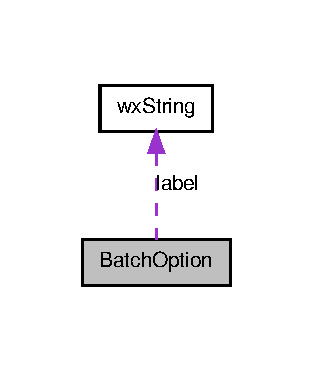
\includegraphics[width=150pt]{structBatchOption__coll__graph}
\end{center}
\end{figure}
\subsection*{Public Member Functions}
\begin{DoxyCompactItemize}
\item 
\hypertarget{structBatchOption_aa639871692215e775a06995c4fe1b108}{
\hyperlink{structBatchOption_aa639871692215e775a06995c4fe1b108}{BatchOption} ()}
\label{structBatchOption_aa639871692215e775a06995c4fe1b108}

\begin{DoxyCompactList}\small\item\em Default constructor. \item\end{DoxyCompactList}\item 
\hyperlink{structBatchOption_af1c023f85fa9f2faac1fe8898ad9895f}{BatchOption} (const \hyperlink{classwxString}{wxString} \&lab, bool sel, int id)
\end{DoxyCompactItemize}
\subsection*{Public Attributes}
\begin{DoxyCompactItemize}
\item 
\hypertarget{structBatchOption_a6a940d6c48fe05f9e2644f7fae620ead}{
\hyperlink{classwxString}{wxString} {\bfseries label}}
\label{structBatchOption_a6a940d6c48fe05f9e2644f7fae620ead}

\item 
\hypertarget{structBatchOption_a10bc2219640a36fb958d12a04e6aa788}{
bool \hyperlink{structBatchOption_a10bc2219640a36fb958d12a04e6aa788}{selection}}
\label{structBatchOption_a10bc2219640a36fb958d12a04e6aa788}

\begin{DoxyCompactList}\small\item\em Checkbox label. \item\end{DoxyCompactList}\item 
\hypertarget{structBatchOption_ad2ed1257616372c9ea259eab2476b4b1}{
int \hyperlink{structBatchOption_ad2ed1257616372c9ea259eab2476b4b1}{index}}
\label{structBatchOption_ad2ed1257616372c9ea259eab2476b4b1}

\begin{DoxyCompactList}\small\item\em Checkbox status. \item\end{DoxyCompactList}\end{DoxyCompactItemize}


\subsection{Detailed Description}
small struct representing a batch dialog option 

\subsection{Constructor \& Destructor Documentation}
\hypertarget{structBatchOption_af1c023f85fa9f2faac1fe8898ad9895f}{
\index{BatchOption@{BatchOption}!BatchOption@{BatchOption}}
\index{BatchOption@{BatchOption}!BatchOption@{BatchOption}}
\subsubsection[{BatchOption}]{\setlength{\rightskip}{0pt plus 5cm}BatchOption::BatchOption (
\begin{DoxyParamCaption}
\item[{const {\bf wxString} \&}]{lab, }
\item[{bool}]{sel, }
\item[{int}]{id}
\end{DoxyParamCaption}
)\hspace{0.3cm}{\ttfamily  \mbox{[}inline\mbox{]}}}}
\label{structBatchOption_af1c023f85fa9f2faac1fe8898ad9895f}
Constructor 
\begin{DoxyParams}{Parameters}
{\em lab} & Checkbox label \\
\hline
{\em sel} & Checkbox status \\
\hline
{\em id} & Index in dialog \\
\hline
\end{DoxyParams}


The documentation for this struct was generated from the following file:\begin{DoxyCompactItemize}
\item 
src/app/dlgs/\hyperlink{smalldlgs_8h}{smalldlgs.h}\end{DoxyCompactItemize}

\hypertarget{classChannel}{
\section{Channel Class Reference}
\label{classChannel}\index{Channel@{Channel}}
}


A \hyperlink{classChannel}{Channel} contains several data \hyperlink{classSection}{Sections } representing observations of the same physical quantity.  




{\ttfamily \#include $<$channel.h$>$}



Collaboration diagram for Channel:
\nopagebreak
\begin{figure}[H]
\begin{center}
\leavevmode
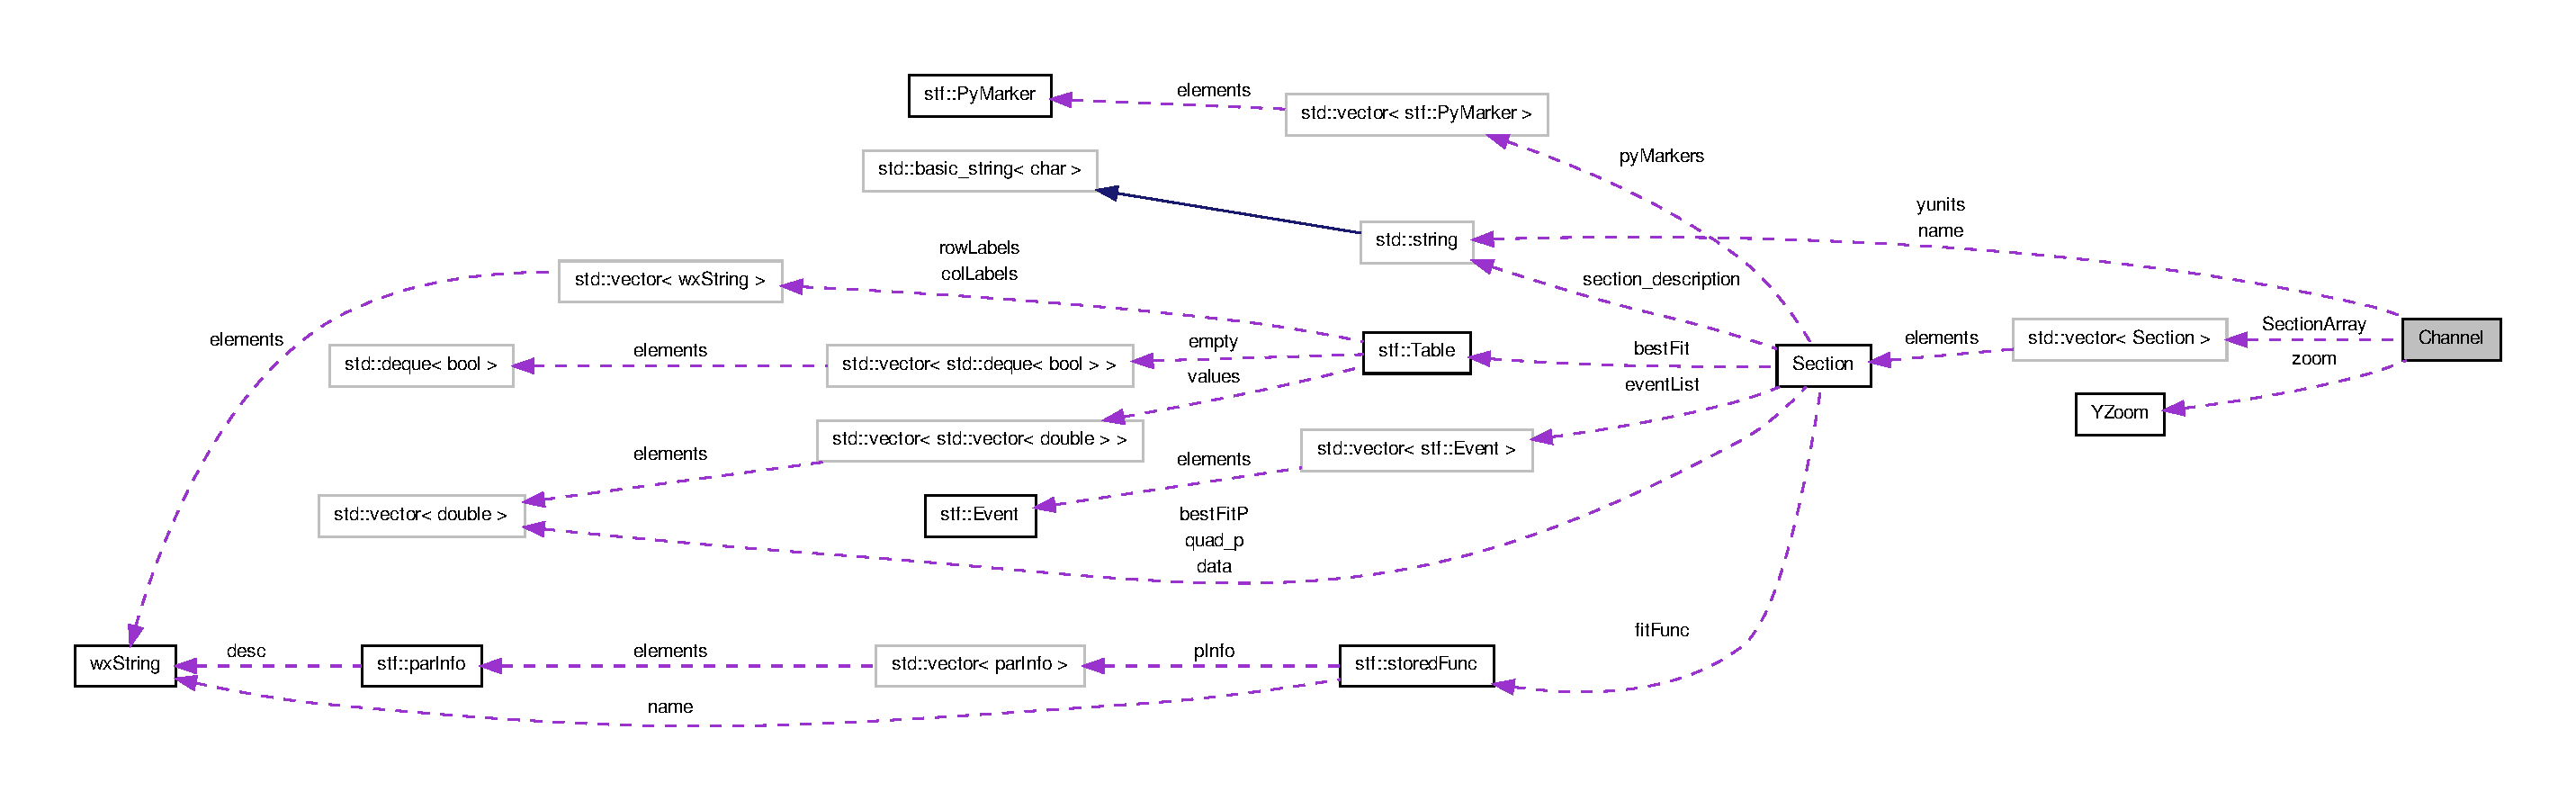
\includegraphics[width=400pt]{classChannel__coll__graph}
\end{center}
\end{figure}
\subsection*{Public Member Functions}
\begin{DoxyCompactItemize}
\item 
\hypertarget{classChannel_a130abb5b562e98a8c700026f6e328118}{
\hyperlink{classChannel_a130abb5b562e98a8c700026f6e328118}{Channel} (void)}
\label{classChannel_a130abb5b562e98a8c700026f6e328118}

\begin{DoxyCompactList}\small\item\em Default constructor. \item\end{DoxyCompactList}\item 
\hyperlink{classChannel_ad23e275f306c9044089dc1785f75ae52}{Channel} (const \hyperlink{classSection}{Section} \&c\_\-Section)
\begin{DoxyCompactList}\small\item\em Constructor. \item\end{DoxyCompactList}\item 
\hyperlink{classChannel_ab8404b525bf98a610dca014613ed85f2}{Channel} (const std::vector$<$ \hyperlink{classSection}{Section} $>$ \&SectionList)
\begin{DoxyCompactList}\small\item\em Constructor. \item\end{DoxyCompactList}\item 
\hyperlink{classChannel_acdf766293ad403862cbe57693b088b0d}{Channel} (std::size\_\-t c\_\-n\_\-sections, std::size\_\-t section\_\-size=0)
\begin{DoxyCompactList}\small\item\em Constructor. \item\end{DoxyCompactList}\item 
\hypertarget{classChannel_a5f15ebd302464069f1a9e3f0ded14482}{
\hyperlink{classChannel_a5f15ebd302464069f1a9e3f0ded14482}{$\sim$Channel} ()}
\label{classChannel_a5f15ebd302464069f1a9e3f0ded14482}

\begin{DoxyCompactList}\small\item\em Destructor. \item\end{DoxyCompactList}\item 
\hyperlink{classSection}{Section} \& \hyperlink{classChannel_a00bfc4162f9a4febff18bd32db7ba238}{operator\mbox{[}$\,$\mbox{]}} (std::size\_\-t at\_\-)
\begin{DoxyCompactList}\small\item\em Unchecked access to a section (read and write) \item\end{DoxyCompactList}\item 
const \hyperlink{classSection}{Section} \& \hyperlink{classChannel_a507d1567e157f080c259b71c8ff214d6}{operator\mbox{[}$\,$\mbox{]}} (std::size\_\-t at\_\-) const 
\begin{DoxyCompactList}\small\item\em Unchecked access to a section (read-\/only) \item\end{DoxyCompactList}\item 
const std::string \& \hyperlink{classChannel_a009b30c9871d77b306d0c42986a1869a}{GetChannelName} () const 
\begin{DoxyCompactList}\small\item\em Retrieves the channel name. \item\end{DoxyCompactList}\item 
const std::string \& \hyperlink{classChannel_a808344243b3730730e0c541d529b803d}{GetYUnits} () const 
\begin{DoxyCompactList}\small\item\em Retrieves the y units string. \item\end{DoxyCompactList}\item 
size\_\-t \hyperlink{classChannel_a85706062035b7c436b41695e3a1fe0f8}{size} () const 
\begin{DoxyCompactList}\small\item\em Retrieves the size of the section array. \item\end{DoxyCompactList}\item 
const \hyperlink{classSection}{Section} \& \hyperlink{classChannel_a5c3ee4edf1450054f99d67413d5ff7c6}{at} (std::size\_\-t at\_\-) const 
\begin{DoxyCompactList}\small\item\em Range-\/checked access to a section (read-\/only). \item\end{DoxyCompactList}\item 
\hyperlink{classSection}{Section} \& \hyperlink{classChannel_a4e0a0e63c39b5a593ce970e141a0a3d3}{at} (std::size\_\-t at\_\-)
\begin{DoxyCompactList}\small\item\em Range-\/checked access to a section (read and write). \item\end{DoxyCompactList}\item 
const std::vector$<$ \hyperlink{classSection}{Section} $>$ \& \hyperlink{classChannel_ae22f828ce5bea9ca4ccb7787072e0585}{get} () const 
\begin{DoxyCompactList}\small\item\em Low-\/level access to the section array (read-\/only). \item\end{DoxyCompactList}\item 
std::vector$<$ \hyperlink{classSection}{Section} $>$ \& \hyperlink{classChannel_a246087dd85eaa37347437b6d2d0e51a8}{get} ()
\begin{DoxyCompactList}\small\item\em Low-\/level access to the section array (read and write). \item\end{DoxyCompactList}\item 
const \hyperlink{classYZoom}{YZoom} \& \hyperlink{classChannel_a99998581e71361e5a06f79e7fbb0303e}{GetYZoom} ()
\begin{DoxyCompactList}\small\item\em Returns the current zoom settings for this channel (read-\/only). \item\end{DoxyCompactList}\item 
\hyperlink{classYZoom}{YZoom} \& \hyperlink{classChannel_a3995ccf99ce0031c7d2510d5444b8999}{GetYZoomW} ()
\begin{DoxyCompactList}\small\item\em Returns the current zoom settings for this channel (read \& write). \item\end{DoxyCompactList}\item 
void \hyperlink{classChannel_ac1816100ed2bf3b68f36872138c8d721}{SetChannelName} (const std::string \&value)
\begin{DoxyCompactList}\small\item\em Sets the channel name. \item\end{DoxyCompactList}\item 
void \hyperlink{classChannel_a70e87deb5f9e16c019ee4f80615d0a2e}{SetYUnits} (const std::string \&value)
\begin{DoxyCompactList}\small\item\em Sets the y units string. \item\end{DoxyCompactList}\item 
void \hyperlink{classChannel_ae60ae41702c7ee29ecfc6f4e602266e7}{InsertSection} (const \hyperlink{classSection}{Section} \&c\_\-Section, std::size\_\-t pos)
\begin{DoxyCompactList}\small\item\em Inserts a section at the given position, overwriting anything that's currently stored at that position. \item\end{DoxyCompactList}\item 
void \hyperlink{classChannel_a6ed41e506c3a975b7a1e9776a38e3504}{resize} (std::size\_\-t newSize)
\begin{DoxyCompactList}\small\item\em Resize the section array. \item\end{DoxyCompactList}\item 
void \hyperlink{classChannel_a904d1019726e0fb75d7422874c941e13}{reserve} (std::size\_\-t resSize)
\begin{DoxyCompactList}\small\item\em Reserve memory for a number of sections. \item\end{DoxyCompactList}\end{DoxyCompactItemize}


\subsection{Detailed Description}
A \hyperlink{classChannel}{Channel} contains several data \hyperlink{classSection}{Sections } representing observations of the same physical quantity. 

\subsection{Constructor \& Destructor Documentation}
\hypertarget{classChannel_ad23e275f306c9044089dc1785f75ae52}{
\index{Channel@{Channel}!Channel@{Channel}}
\index{Channel@{Channel}!Channel@{Channel}}
\subsubsection[{Channel}]{\setlength{\rightskip}{0pt plus 5cm}Channel::Channel (
\begin{DoxyParamCaption}
\item[{const {\bf Section} \&}]{c\_\-Section}
\end{DoxyParamCaption}
)\hspace{0.3cm}{\ttfamily  \mbox{[}explicit\mbox{]}}}}
\label{classChannel_ad23e275f306c9044089dc1785f75ae52}


Constructor. 


\begin{DoxyParams}{Parameters}
{\em c\_\-Section} & A single section from which to construct the channel \\
\hline
\end{DoxyParams}
\hypertarget{classChannel_ab8404b525bf98a610dca014613ed85f2}{
\index{Channel@{Channel}!Channel@{Channel}}
\index{Channel@{Channel}!Channel@{Channel}}
\subsubsection[{Channel}]{\setlength{\rightskip}{0pt plus 5cm}Channel::Channel (
\begin{DoxyParamCaption}
\item[{const std::vector$<$ {\bf Section} $>$ \&}]{SectionList}
\end{DoxyParamCaption}
)\hspace{0.3cm}{\ttfamily  \mbox{[}explicit\mbox{]}}}}
\label{classChannel_ab8404b525bf98a610dca014613ed85f2}


Constructor. 


\begin{DoxyParams}{Parameters}
{\em SectionList} & A vector of Sections from which to construct the channel \\
\hline
\end{DoxyParams}
\hypertarget{classChannel_acdf766293ad403862cbe57693b088b0d}{
\index{Channel@{Channel}!Channel@{Channel}}
\index{Channel@{Channel}!Channel@{Channel}}
\subsubsection[{Channel}]{\setlength{\rightskip}{0pt plus 5cm}Channel::Channel (
\begin{DoxyParamCaption}
\item[{std::size\_\-t}]{c\_\-n\_\-sections, }
\item[{std::size\_\-t}]{section\_\-size = {\ttfamily 0}}
\end{DoxyParamCaption}
)\hspace{0.3cm}{\ttfamily  \mbox{[}explicit\mbox{]}}}}
\label{classChannel_acdf766293ad403862cbe57693b088b0d}


Constructor. 

Setting the number of sections at construction time will avoid unnecessary memory re-\/allocations. 
\begin{DoxyParams}{Parameters}
{\em c\_\-n\_\-sections} & The number of sections. \\
\hline
{\em section\_\-size} & Initial section size. Will serve additional re-\/alocations if known at construction time. \\
\hline
\end{DoxyParams}


\subsection{Member Function Documentation}
\hypertarget{classChannel_a5c3ee4edf1450054f99d67413d5ff7c6}{
\index{Channel@{Channel}!at@{at}}
\index{at@{at}!Channel@{Channel}}
\subsubsection[{at}]{\setlength{\rightskip}{0pt plus 5cm}const {\bf Section}\& Channel::at (
\begin{DoxyParamCaption}
\item[{std::size\_\-t}]{at\_\-}
\end{DoxyParamCaption}
) const}}
\label{classChannel_a5c3ee4edf1450054f99d67413d5ff7c6}


Range-\/checked access to a section (read-\/only). 

Will throw std::out\_\-of\_\-range if out of range. 
\begin{DoxyParams}{Parameters}
{\em at\_\-} & The index of the section. \\
\hline
\end{DoxyParams}
\begin{DoxyReturn}{Returns}
The section at index at\_\-. 
\end{DoxyReturn}
\hypertarget{classChannel_a4e0a0e63c39b5a593ce970e141a0a3d3}{
\index{Channel@{Channel}!at@{at}}
\index{at@{at}!Channel@{Channel}}
\subsubsection[{at}]{\setlength{\rightskip}{0pt plus 5cm}{\bf Section}\& Channel::at (
\begin{DoxyParamCaption}
\item[{std::size\_\-t}]{at\_\-}
\end{DoxyParamCaption}
)}}
\label{classChannel_a4e0a0e63c39b5a593ce970e141a0a3d3}


Range-\/checked access to a section (read and write). 

Will throw std::out\_\-of\_\-range if out of range. 
\begin{DoxyParams}{Parameters}
{\em at\_\-} & The index of the section. \\
\hline
\end{DoxyParams}
\begin{DoxyReturn}{Returns}
The section at index at\_\-. 
\end{DoxyReturn}
\hypertarget{classChannel_ae22f828ce5bea9ca4ccb7787072e0585}{
\index{Channel@{Channel}!get@{get}}
\index{get@{get}!Channel@{Channel}}
\subsubsection[{get}]{\setlength{\rightskip}{0pt plus 5cm}const std::vector$<$ {\bf Section} $>$\& Channel::get (
\begin{DoxyParamCaption}
{}
\end{DoxyParamCaption}
) const\hspace{0.3cm}{\ttfamily  \mbox{[}inline\mbox{]}}}}
\label{classChannel_ae22f828ce5bea9ca4ccb7787072e0585}


Low-\/level access to the section array (read-\/only). 

\begin{DoxyReturn}{Returns}
The vector containing the sections. 
\end{DoxyReturn}
\hypertarget{classChannel_a246087dd85eaa37347437b6d2d0e51a8}{
\index{Channel@{Channel}!get@{get}}
\index{get@{get}!Channel@{Channel}}
\subsubsection[{get}]{\setlength{\rightskip}{0pt plus 5cm}std::vector$<$ {\bf Section} $>$\& Channel::get (
\begin{DoxyParamCaption}
{}
\end{DoxyParamCaption}
)\hspace{0.3cm}{\ttfamily  \mbox{[}inline\mbox{]}}}}
\label{classChannel_a246087dd85eaa37347437b6d2d0e51a8}


Low-\/level access to the section array (read and write). 

\begin{DoxyReturn}{Returns}
The vector containing the sections. 
\end{DoxyReturn}
\hypertarget{classChannel_a009b30c9871d77b306d0c42986a1869a}{
\index{Channel@{Channel}!GetChannelName@{GetChannelName}}
\index{GetChannelName@{GetChannelName}!Channel@{Channel}}
\subsubsection[{GetChannelName}]{\setlength{\rightskip}{0pt plus 5cm}const std::string\& Channel::GetChannelName (
\begin{DoxyParamCaption}
{}
\end{DoxyParamCaption}
) const\hspace{0.3cm}{\ttfamily  \mbox{[}inline\mbox{]}}}}
\label{classChannel_a009b30c9871d77b306d0c42986a1869a}


Retrieves the channel name. 

\begin{DoxyReturn}{Returns}
The channel name. 
\end{DoxyReturn}
\hypertarget{classChannel_a808344243b3730730e0c541d529b803d}{
\index{Channel@{Channel}!GetYUnits@{GetYUnits}}
\index{GetYUnits@{GetYUnits}!Channel@{Channel}}
\subsubsection[{GetYUnits}]{\setlength{\rightskip}{0pt plus 5cm}const std::string\& Channel::GetYUnits (
\begin{DoxyParamCaption}
{}
\end{DoxyParamCaption}
) const\hspace{0.3cm}{\ttfamily  \mbox{[}inline\mbox{]}}}}
\label{classChannel_a808344243b3730730e0c541d529b803d}


Retrieves the y units string. 

\begin{DoxyReturn}{Returns}
The y units string. 
\end{DoxyReturn}
\hypertarget{classChannel_a99998581e71361e5a06f79e7fbb0303e}{
\index{Channel@{Channel}!GetYZoom@{GetYZoom}}
\index{GetYZoom@{GetYZoom}!Channel@{Channel}}
\subsubsection[{GetYZoom}]{\setlength{\rightskip}{0pt plus 5cm}const {\bf YZoom}\& Channel::GetYZoom (
\begin{DoxyParamCaption}
{}
\end{DoxyParamCaption}
)\hspace{0.3cm}{\ttfamily  \mbox{[}inline\mbox{]}}}}
\label{classChannel_a99998581e71361e5a06f79e7fbb0303e}


Returns the current zoom settings for this channel (read-\/only). 

\begin{DoxyReturn}{Returns}
The current zoom settings. 
\end{DoxyReturn}
\hypertarget{classChannel_a3995ccf99ce0031c7d2510d5444b8999}{
\index{Channel@{Channel}!GetYZoomW@{GetYZoomW}}
\index{GetYZoomW@{GetYZoomW}!Channel@{Channel}}
\subsubsection[{GetYZoomW}]{\setlength{\rightskip}{0pt plus 5cm}{\bf YZoom}\& Channel::GetYZoomW (
\begin{DoxyParamCaption}
{}
\end{DoxyParamCaption}
)\hspace{0.3cm}{\ttfamily  \mbox{[}inline\mbox{]}}}}
\label{classChannel_a3995ccf99ce0031c7d2510d5444b8999}


Returns the current zoom settings for this channel (read \& write). 

\begin{DoxyReturn}{Returns}
The current zoom settings. 
\end{DoxyReturn}
\hypertarget{classChannel_ae60ae41702c7ee29ecfc6f4e602266e7}{
\index{Channel@{Channel}!InsertSection@{InsertSection}}
\index{InsertSection@{InsertSection}!Channel@{Channel}}
\subsubsection[{InsertSection}]{\setlength{\rightskip}{0pt plus 5cm}void Channel::InsertSection (
\begin{DoxyParamCaption}
\item[{const {\bf Section} \&}]{c\_\-Section, }
\item[{std::size\_\-t}]{pos}
\end{DoxyParamCaption}
)}}
\label{classChannel_ae60ae41702c7ee29ecfc6f4e602266e7}


Inserts a section at the given position, overwriting anything that's currently stored at that position. 

Meant to be used after constructing with \hyperlink{classChannel}{Channel}(const unsigned int\& c\_\-n\_\-sections\}. The section array size has to be larger than pos because it won't be resized. Will throw std::out\_\-of\_\-range if out of range. 
\begin{DoxyParams}{Parameters}
{\em c\_\-Section} & The section to be inserted. \\
\hline
{\em pos} & The position at which to insert the section. \\
\hline
\end{DoxyParams}
\hypertarget{classChannel_a507d1567e157f080c259b71c8ff214d6}{
\index{Channel@{Channel}!operator\mbox{[}\mbox{]}@{operator[]}}
\index{operator\mbox{[}\mbox{]}@{operator[]}!Channel@{Channel}}
\subsubsection[{operator[]}]{\setlength{\rightskip}{0pt plus 5cm}const {\bf Section}\& Channel::operator\mbox{[}$\,$\mbox{]} (
\begin{DoxyParamCaption}
\item[{std::size\_\-t}]{at\_\-}
\end{DoxyParamCaption}
) const\hspace{0.3cm}{\ttfamily  \mbox{[}inline\mbox{]}}}}
\label{classChannel_a507d1567e157f080c259b71c8ff214d6}


Unchecked access to a section (read-\/only) 

Use \hyperlink{classChannel_a5c3ee4edf1450054f99d67413d5ff7c6}{at()} for range-\/checked access. 
\begin{DoxyParams}{Parameters}
{\em at\_\-} & The section index. \\
\hline
\end{DoxyParams}
\begin{DoxyReturn}{Returns}
The section at index at\_\-. 
\end{DoxyReturn}
\hypertarget{classChannel_a00bfc4162f9a4febff18bd32db7ba238}{
\index{Channel@{Channel}!operator\mbox{[}\mbox{]}@{operator[]}}
\index{operator\mbox{[}\mbox{]}@{operator[]}!Channel@{Channel}}
\subsubsection[{operator[]}]{\setlength{\rightskip}{0pt plus 5cm}{\bf Section}\& Channel::operator\mbox{[}$\,$\mbox{]} (
\begin{DoxyParamCaption}
\item[{std::size\_\-t}]{at\_\-}
\end{DoxyParamCaption}
)\hspace{0.3cm}{\ttfamily  \mbox{[}inline\mbox{]}}}}
\label{classChannel_a00bfc4162f9a4febff18bd32db7ba238}


Unchecked access to a section (read and write) 

Use \hyperlink{classChannel_a5c3ee4edf1450054f99d67413d5ff7c6}{at()} for range-\/checked access. 
\begin{DoxyParams}{Parameters}
{\em at\_\-} & The section index. \\
\hline
\end{DoxyParams}
\begin{DoxyReturn}{Returns}
The section at index at\_\-. 
\end{DoxyReturn}
\hypertarget{classChannel_a904d1019726e0fb75d7422874c941e13}{
\index{Channel@{Channel}!reserve@{reserve}}
\index{reserve@{reserve}!Channel@{Channel}}
\subsubsection[{reserve}]{\setlength{\rightskip}{0pt plus 5cm}void Channel::reserve (
\begin{DoxyParamCaption}
\item[{std::size\_\-t}]{resSize}
\end{DoxyParamCaption}
)\hspace{0.3cm}{\ttfamily  \mbox{[}inline\mbox{]}}}}
\label{classChannel_a904d1019726e0fb75d7422874c941e13}


Reserve memory for a number of sections. 

This will avoid unnecessary memory re-\/allocations. 
\begin{DoxyParams}{Parameters}
{\em resSize} & The number of sections to reserve memory for. \\
\hline
\end{DoxyParams}
\hypertarget{classChannel_a6ed41e506c3a975b7a1e9776a38e3504}{
\index{Channel@{Channel}!resize@{resize}}
\index{resize@{resize}!Channel@{Channel}}
\subsubsection[{resize}]{\setlength{\rightskip}{0pt plus 5cm}void Channel::resize (
\begin{DoxyParamCaption}
\item[{std::size\_\-t}]{newSize}
\end{DoxyParamCaption}
)\hspace{0.3cm}{\ttfamily  \mbox{[}inline\mbox{]}}}}
\label{classChannel_a6ed41e506c3a975b7a1e9776a38e3504}


Resize the section array. 


\begin{DoxyParams}{Parameters}
{\em newSize} & The new number of sections. \\
\hline
\end{DoxyParams}
\hypertarget{classChannel_ac1816100ed2bf3b68f36872138c8d721}{
\index{Channel@{Channel}!SetChannelName@{SetChannelName}}
\index{SetChannelName@{SetChannelName}!Channel@{Channel}}
\subsubsection[{SetChannelName}]{\setlength{\rightskip}{0pt plus 5cm}void Channel::SetChannelName (
\begin{DoxyParamCaption}
\item[{const std::string \&}]{value}
\end{DoxyParamCaption}
)\hspace{0.3cm}{\ttfamily  \mbox{[}inline\mbox{]}}}}
\label{classChannel_ac1816100ed2bf3b68f36872138c8d721}


Sets the channel name. 


\begin{DoxyParams}{Parameters}
{\em value} & The channel name. \\
\hline
\end{DoxyParams}
\hypertarget{classChannel_a70e87deb5f9e16c019ee4f80615d0a2e}{
\index{Channel@{Channel}!SetYUnits@{SetYUnits}}
\index{SetYUnits@{SetYUnits}!Channel@{Channel}}
\subsubsection[{SetYUnits}]{\setlength{\rightskip}{0pt plus 5cm}void Channel::SetYUnits (
\begin{DoxyParamCaption}
\item[{const std::string \&}]{value}
\end{DoxyParamCaption}
)\hspace{0.3cm}{\ttfamily  \mbox{[}inline\mbox{]}}}}
\label{classChannel_a70e87deb5f9e16c019ee4f80615d0a2e}


Sets the y units string. 


\begin{DoxyParams}{Parameters}
{\em value} & The new y units string. \\
\hline
\end{DoxyParams}
\hypertarget{classChannel_a85706062035b7c436b41695e3a1fe0f8}{
\index{Channel@{Channel}!size@{size}}
\index{size@{size}!Channel@{Channel}}
\subsubsection[{size}]{\setlength{\rightskip}{0pt plus 5cm}size\_\-t Channel::size (
\begin{DoxyParamCaption}
{}
\end{DoxyParamCaption}
) const\hspace{0.3cm}{\ttfamily  \mbox{[}inline\mbox{]}}}}
\label{classChannel_a85706062035b7c436b41695e3a1fe0f8}


Retrieves the size of the section array. 

\begin{DoxyReturn}{Returns}
The size of the section array. 
\end{DoxyReturn}


The documentation for this class was generated from the following file:\begin{DoxyCompactItemize}
\item 
src/core/\hyperlink{channel_8h}{channel.h}\end{DoxyCompactItemize}

\hypertarget{classRecording}{
\section{Recording Class Reference}
\label{classRecording}\index{Recording@{Recording}}
}


Represents the data within a file.  




{\ttfamily \#include $<$recording.h$>$}



Inheritance diagram for Recording:
\nopagebreak
\begin{figure}[H]
\begin{center}
\leavevmode
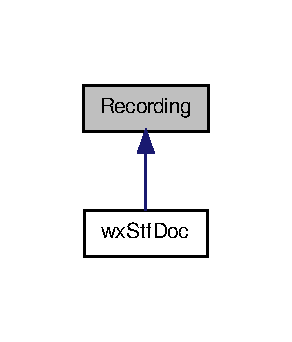
\includegraphics[width=140pt]{classRecording__inherit__graph}
\end{center}
\end{figure}


Collaboration diagram for Recording:
\nopagebreak
\begin{figure}[H]
\begin{center}
\leavevmode
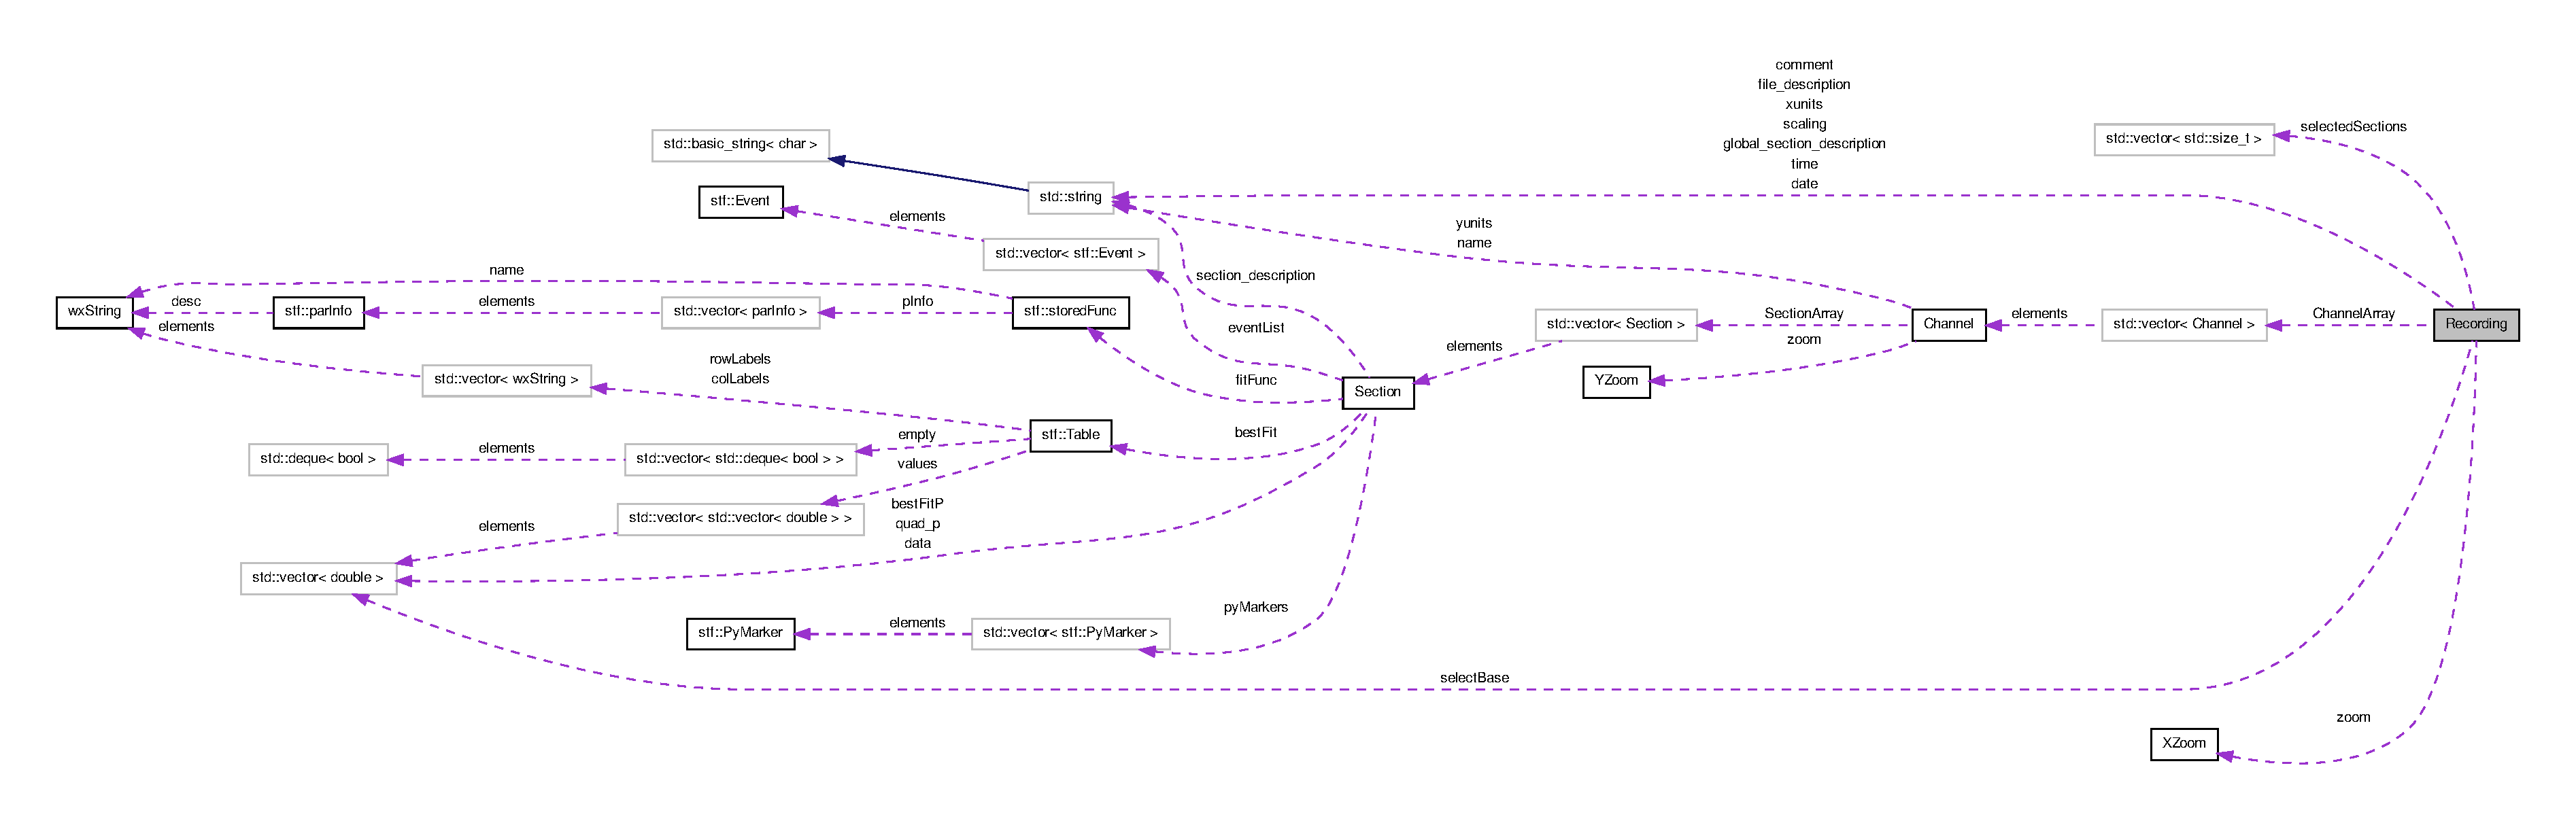
\includegraphics[width=400pt]{classRecording__coll__graph}
\end{center}
\end{figure}
\subsection*{Public Member Functions}
\begin{DoxyCompactItemize}
\item 
\hypertarget{classRecording_a270f855f9547078427135d75854cd7c6}{
\hyperlink{classRecording_a270f855f9547078427135d75854cd7c6}{Recording} ()}
\label{classRecording_a270f855f9547078427135d75854cd7c6}

\begin{DoxyCompactList}\small\item\em Default constuctor. \item\end{DoxyCompactList}\item 
\hyperlink{classRecording_ac1219247e33bfd916d32d00d4fc86051}{Recording} (const \hyperlink{classChannel}{Channel} \&c\_\-Channel)
\begin{DoxyCompactList}\small\item\em Constructor. \item\end{DoxyCompactList}\item 
\hyperlink{classRecording_ae1d7a66d03e2754c9ecaa6920d28f672}{Recording} (const std::vector$<$ \hyperlink{classChannel}{Channel} $>$ \&ChannelList)
\begin{DoxyCompactList}\small\item\em Constructor. \item\end{DoxyCompactList}\item 
\hyperlink{classRecording_a35b98e700d186598e8a1aa6c34b47352}{Recording} (std::size\_\-t c\_\-n\_\-channels, std::size\_\-t c\_\-n\_\-sections=0, std::size\_\-t c\_\-n\_\-points=0)
\begin{DoxyCompactList}\small\item\em Constructor. \item\end{DoxyCompactList}\item 
\hypertarget{classRecording_aed6604f8b6f495f7570c9844290add2a}{
virtual \hyperlink{classRecording_aed6604f8b6f495f7570c9844290add2a}{$\sim$Recording} ()}
\label{classRecording_aed6604f8b6f495f7570c9844290add2a}

\begin{DoxyCompactList}\small\item\em Destructor. \item\end{DoxyCompactList}\item 
std::size\_\-t \hyperlink{classRecording_a63e3ccf892626f33082c82de2897ed08}{GetChannelSize} (std::size\_\-t n\_\-channel) const 
\begin{DoxyCompactList}\small\item\em Retrieves the number of sections in a channel. \item\end{DoxyCompactList}\item 
const std::vector$<$ \hyperlink{classChannel}{Channel} $>$ \& \hyperlink{classRecording_a5156de9f9f9bb71b0b39de838a0031f2}{get} () const 
\begin{DoxyCompactList}\small\item\em Retrieves the channels (read-\/only). \item\end{DoxyCompactList}\item 
std::vector$<$ \hyperlink{classChannel}{Channel} $>$ \& \hyperlink{classRecording_aeb8d43d6ee2fed242fe49e1a238b2ae2}{get} ()
\begin{DoxyCompactList}\small\item\em Retrieves the channels (read and write). \item\end{DoxyCompactList}\item 
const std::string \& \hyperlink{classRecording_a6070a9a8cf66efbb6ed5e1e0c7fc0263}{GetFileDescription} () const 
\begin{DoxyCompactList}\small\item\em Retrieves the file description. \item\end{DoxyCompactList}\item 
const std::string \& \hyperlink{classRecording_a44d232789cf4f3918dd61baafd4b7071}{GetGlobalSectionDescription} () const 
\begin{DoxyCompactList}\small\item\em Retrieves the common section description. \item\end{DoxyCompactList}\item 
const std::string \& \hyperlink{classRecording_a83060d2146fa05eacfee71ffaa17caa5}{GetScaling} () const 
\begin{DoxyCompactList}\small\item\em Retrieves the scaling as a string. \item\end{DoxyCompactList}\item 
const std::string \& \hyperlink{classRecording_a9ace50171c2e433cea86c52500fd7d13}{GetTime} () const 
\begin{DoxyCompactList}\small\item\em Retrieves the time of recording as a string. \item\end{DoxyCompactList}\item 
const std::string \& \hyperlink{classRecording_a379e654d9603b4fa304dadb1f3f7e7db}{GetDate} () const 
\begin{DoxyCompactList}\small\item\em Retrieves the date of recording as a string. \item\end{DoxyCompactList}\item 
const std::string \& \hyperlink{classRecording_a7ab947f6584fc5e4a07074fca60b9be9}{GetComment} () const 
\begin{DoxyCompactList}\small\item\em Retrieves a comment string. \item\end{DoxyCompactList}\item 
const std::string \& \hyperlink{classRecording_a2de7ff0583d303bfe88d19864d924750}{GetXUnits} () const 
\begin{DoxyCompactList}\small\item\em Retrieves the x units. \item\end{DoxyCompactList}\item 
std::size\_\-t \hyperlink{classRecording_ae85d90e4ab8508aa23649a168ccb0115}{size} () const 
\begin{DoxyCompactList}\small\item\em Retrieves the size of the channel array. \item\end{DoxyCompactList}\item 
double \hyperlink{classRecording_a7c68162cb02488225eb99ddb9a422917}{GetXScale} () const 
\begin{DoxyCompactList}\small\item\em Retrieves the x scaling (sampling interval). \item\end{DoxyCompactList}\item 
double \hyperlink{classRecording_a077940a80024c2107c157864f957c432}{GetSR} () const 
\begin{DoxyCompactList}\small\item\em Retrieves the sampling rate ( 1 / x-\/scale ) \item\end{DoxyCompactList}\item 
const \hyperlink{classChannel}{Channel} \& \hyperlink{classRecording_a5c79855f2de693656909f3ea9b43b943}{at} (std::size\_\-t n\_\-c) const 
\begin{DoxyCompactList}\small\item\em Range-\/checked access to a channel (read-\/only). \item\end{DoxyCompactList}\item 
\hyperlink{classChannel}{Channel} \& \hyperlink{classRecording_a0a788926cbef764f62fca685b92a2e15}{at} (std::size\_\-t n\_\-c)
\begin{DoxyCompactList}\small\item\em Range-\/checked access to a channel (read and write). \item\end{DoxyCompactList}\item 
std::size\_\-t \hyperlink{classRecording_ad216e46012a6b7630d4baeac15b110a9}{GetCurCh} () const 
\begin{DoxyCompactList}\small\item\em Retrieves the index of the current channel. \item\end{DoxyCompactList}\item 
std::size\_\-t \hyperlink{classRecording_ab870119d64fd52d656cb4d7882b20fab}{GetSecCh} () const 
\begin{DoxyCompactList}\small\item\em Retrieves the index of the second channel. \item\end{DoxyCompactList}\item 
std::size\_\-t \hyperlink{classRecording_aa6b87b7a6e22b86f1fe200c278fe65a6}{GetCurSec} () const 
\begin{DoxyCompactList}\small\item\em Retrieves the index of the current section. \item\end{DoxyCompactList}\item 
std::size\_\-t \hyperlink{classRecording_a11d7a0afbb103e89cdefd0c60a1e1d9f}{GetMeasCursor} () const 
\begin{DoxyCompactList}\small\item\em Retrieves the position of the measurement cursor (crosshair). \item\end{DoxyCompactList}\item 
std::size\_\-t \hyperlink{classRecording_a2f7d618c4debfa908e10e30512afb798}{GetBaseBeg} () const 
\begin{DoxyCompactList}\small\item\em Retrieves the position of the left baseline cursor. \item\end{DoxyCompactList}\item 
std::size\_\-t \hyperlink{classRecording_ad51bce5e89ac87cdc818e341eedef208}{GetBaseEnd} () const 
\begin{DoxyCompactList}\small\item\em Retrieves the position of the right baseline cursor. \item\end{DoxyCompactList}\item 
std::size\_\-t \hyperlink{classRecording_ae24bbad06dda64884b11763fdc28deec}{GetPeakBeg} () const 
\begin{DoxyCompactList}\small\item\em Retrieves the position of the left peak cursor. \item\end{DoxyCompactList}\item 
std::size\_\-t \hyperlink{classRecording_a49b39637356c545c2a3520d1865a5588}{GetPeakEnd} () const 
\begin{DoxyCompactList}\small\item\em Retrieves the position of the right peak cursor. \item\end{DoxyCompactList}\item 
std::size\_\-t \hyperlink{classRecording_ad54ad852c63945418ce8fad67cebd803}{GetFitBeg} () const 
\begin{DoxyCompactList}\small\item\em Retrieves the position of the left fitting cursor. \item\end{DoxyCompactList}\item 
std::size\_\-t \hyperlink{classRecording_a82f1e579b31a2fbcc6d526050ee919dd}{GetFitEnd} () const 
\begin{DoxyCompactList}\small\item\em Retrieves the position of the right fitting cursor. \item\end{DoxyCompactList}\item 
int \hyperlink{classRecording_aac8ab06e8e054bdb3fda76963a5be2ac}{GetPM} () const 
\begin{DoxyCompactList}\small\item\em Retrieves the number of points used for averaging during peak calculation. \item\end{DoxyCompactList}\item 
double \hyperlink{classRecording_acd1c834b6db0c8c398e4a2b3aa5d18f3}{GetLatencyBeg} () const 
\begin{DoxyCompactList}\small\item\em Retrieves the position of the left latency cursor. \item\end{DoxyCompactList}\item 
double \hyperlink{classRecording_a2022e82ab61364e3e2a68e41bcf616bb}{GetLatencyEnd} () const 
\begin{DoxyCompactList}\small\item\em Retrieves the position of the right latency cursor. \item\end{DoxyCompactList}\item 
double \hyperlink{classRecording_a3d7de67ec49a28bc8797ebeaee4eb35b}{GetLatency} () const 
\begin{DoxyCompactList}\small\item\em Retrieves the latency. \item\end{DoxyCompactList}\item 
double \hyperlink{classRecording_aad7f546bda00fed7c005c64be81a3bf4}{GetT20Real} () const 
\begin{DoxyCompactList}\small\item\em Retrieves the time point at which 20\% of the maximal amplitude have been reached. \item\end{DoxyCompactList}\item 
double \hyperlink{classRecording_ab67e3db7110f63f3a098ec8f75603594}{GetT80Real} () const 
\begin{DoxyCompactList}\small\item\em Retrieves the time point at which 80\% of the maximal amplitude have been reached. \item\end{DoxyCompactList}\item 
double \hyperlink{classRecording_a5798892554031d885319eff5fc72002c}{GetT50LeftReal} () const 
\begin{DoxyCompactList}\small\item\em Retrieves the time point at which 50\% of the maximal amplitude have been reached from the left of the peak. \item\end{DoxyCompactList}\item 
double \hyperlink{classRecording_aa1e0a42814e2e985e38f0a0f43f5dad7}{GetT50RightReal} () const 
\begin{DoxyCompactList}\small\item\em Retrieves the time point at which 50\% of the maximal amplitude have been reached from the right of the peak. \item\end{DoxyCompactList}\item 
double \hyperlink{classRecording_a4a42b50c87111915907d8edd4bbdadfe}{GetT50Y} () const 
\begin{DoxyCompactList}\small\item\em Retrieves the y value at 50\% of the maximal amplitude. \item\end{DoxyCompactList}\item 
double \hyperlink{classRecording_aabad745e2588229871cb5b09727f65dd}{GetMaxRise} () const 
\begin{DoxyCompactList}\small\item\em Retrieves the maximal slope of the rising phase. \item\end{DoxyCompactList}\item 
double \hyperlink{classRecording_a10828c1a1db5f3a452ef6d4558a3cf05}{GetMaxDecay} () const 
\begin{DoxyCompactList}\small\item\em Retrieves the maximal slope of the decaying phase. \item\end{DoxyCompactList}\item 
double \hyperlink{classRecording_a8786f03e5b1de85b2032551d89b3da79}{GetAPMaxRiseT} () const 
\begin{DoxyCompactList}\small\item\em Retrieves the time point of the maximal slope of the rising phase in the second channel. \item\end{DoxyCompactList}\item 
double \hyperlink{classRecording_a2aeab23d129ef86ac4570b253f7c9570}{GetAPMaxT} () const 
\begin{DoxyCompactList}\small\item\em Retrieves the time point of the peak in the second channel. \item\end{DoxyCompactList}\item 
double \hyperlink{classRecording_aae3cfa487a207709e3f77984a02c78a1}{GetAPT50LeftReal} () const 
\begin{DoxyCompactList}\small\item\em Retrieves the time point at which 50\% of the max. amplitude have been reached from the left of the peak in the inactive channel. \item\end{DoxyCompactList}\item 
double \hyperlink{classRecording_a28cc5ced08658608ffd4d0a562f748ec}{GetMaxRiseT} () const 
\begin{DoxyCompactList}\small\item\em Retrieves the time point of the maximal slope during the rising phase. \item\end{DoxyCompactList}\item 
double \hyperlink{classRecording_a1c15a836ced7baf51fa007ade0274309}{GetMaxRiseY} () const 
\begin{DoxyCompactList}\small\item\em Retrieves the y-\/value at the time point of the maximal slope during the rising phase. \item\end{DoxyCompactList}\item 
double \hyperlink{classRecording_a48be6fe2246e3b6d05c1afde144cee7e}{GetMaxDecayT} () const 
\begin{DoxyCompactList}\small\item\em Retrieves the time point of the maximal slope during the decaying phase. \item\end{DoxyCompactList}\item 
double \hyperlink{classRecording_ad50ae196f6f57496eddfde31746d66d2}{GetMaxDecayY} () const 
\begin{DoxyCompactList}\small\item\em Retrieves the y-\/value at the time point of the maximal slope during the decaying phase. \item\end{DoxyCompactList}\item 
double \hyperlink{classRecording_a9864faad555a8045d63a8b7eb1d48a4d}{GetMeasValue} ()
\begin{DoxyCompactList}\small\item\em Retrieves the y-\/value at the measurement cursor (crosshair). Will update measCursor if out of range. \item\end{DoxyCompactList}\item 
double \hyperlink{classRecording_aac9e484d34cd41ee08d03e7d9dffbfc1}{GetPeak} () const 
\begin{DoxyCompactList}\small\item\em Retrieves the peak value. \item\end{DoxyCompactList}\item 
double \hyperlink{classRecording_a71acc241d3c282fde919c8e710876541}{GetBase} () const 
\begin{DoxyCompactList}\small\item\em Retrieves the baseline. \item\end{DoxyCompactList}\item 
double \hyperlink{classRecording_a5d302113fe4b37e0ab373278f3a6d618}{GetAPBase} () const 
\begin{DoxyCompactList}\small\item\em Retrieves the baseline in the second channel. \item\end{DoxyCompactList}\item 
double \hyperlink{classRecording_ae8860f078ef8c5c19f38c234c9690819}{GetBaseSD} () const 
\begin{DoxyCompactList}\small\item\em Retrieves the standard deviation of the baseline. \item\end{DoxyCompactList}\item 
double \hyperlink{classRecording_a60b49830249c73a6d8267b94afcc7fbb}{GetThreshold} () const 
\begin{DoxyCompactList}\small\item\em Retrieves the value at which the threshold slope is crossed. \item\end{DoxyCompactList}\item 
double \hyperlink{classRecording_aa9cf83f451504c4a9a87f3385046ce0a}{GetMaxT} () const 
\begin{DoxyCompactList}\small\item\em Retrieves the time point at which the peak is found. \item\end{DoxyCompactList}\item 
double \hyperlink{classRecording_aa01a720786fb4f989008f8565d98bda0}{GetThrT} () const 
\begin{DoxyCompactList}\small\item\em Retrieves the time point at which the threshold slope is crossed. \item\end{DoxyCompactList}\item 
double \hyperlink{classRecording_ad02ba9ecca6c9559c64748b980cd51ef}{GetRT2080} () const 
\begin{DoxyCompactList}\small\item\em Retrieves the 20 to 80\% rise time. \item\end{DoxyCompactList}\item 
double \hyperlink{classRecording_a9d09f4cec914f37294f392711aff6b5f}{GetHalfDuration} () const 
\begin{DoxyCompactList}\small\item\em Retrieves the full width at half-\/maximal amplitude (\char`\"{}half duration\char`\"{}). \item\end{DoxyCompactList}\item 
double \hyperlink{classRecording_a73c170fcc503cbaf4352a4322129d3f0}{GetSlopeRatio} () const 
\begin{DoxyCompactList}\small\item\em Retrieves ratio of the maximal slopes during the rising and decaying phase. \item\end{DoxyCompactList}\item 
double \hyperlink{classRecording_a6575bf91ef1f6e3cf58e8f75ce3691fe}{GetPSlope} () const 
\begin{DoxyCompactList}\small\item\em Retrieves the value of the Slope. \item\end{DoxyCompactList}\item 
\hyperlink{group__stfgen_ga738f9934a45a9d2d81cb0a3de0375c99}{stf::latency\_\-mode} \hyperlink{classRecording_ae82a0d76aa6454a7187e32399bcd5c8c}{GetLatencyStartMode} () const 
\begin{DoxyCompactList}\small\item\em Retrieves the mode of the latency start cursor. \item\end{DoxyCompactList}\item 
\hyperlink{group__stfgen_ga738f9934a45a9d2d81cb0a3de0375c99}{stf::latency\_\-mode} \hyperlink{classRecording_acef949762142160e2014fcec24aebf32}{GetLatencyEndMode} () const 
\begin{DoxyCompactList}\small\item\em Retrieves the mode of the latency end cursor. \item\end{DoxyCompactList}\item 
\hyperlink{group__stfgen_gae034ed0eec6bdaba3b23d3b2184f799d}{stf::latency\_\-window\_\-mode} \hyperlink{classRecording_a534771ad7f73eaf8c038efdc3887ccda}{GetLatencyWindowMode} () const 
\begin{DoxyCompactList}\small\item\em Retrieves the mode of the latency window. \item\end{DoxyCompactList}\item 
\hyperlink{group__stfgen_gae8845ae2aeaf4b742a905a2a5571fd5a}{stf::direction} \hyperlink{classRecording_af72b0104c87d7a0c4a18bdea1a8d8da2}{GetDirection} () const 
\begin{DoxyCompactList}\small\item\em Retrieves the direction of peak calculations. \item\end{DoxyCompactList}\item 
bool \hyperlink{classRecording_a014bb4c39cb99dcc2e1260666074a8e4}{GetFromBase} () const 
\begin{DoxyCompactList}\small\item\em Indicates whether to use the baseline as a reference for AP kinetics. \item\end{DoxyCompactList}\item 
bool \hyperlink{classRecording_a14025db3c94ecdd8dfcb761512ad74e3}{GetViewCrosshair} () const 
\begin{DoxyCompactList}\small\item\em Indicates whether the measurement cursor (crosshair) value should be shown in the results table. \item\end{DoxyCompactList}\item 
bool \hyperlink{classRecording_ac984785dee334420793862355addd1cc}{GetViewBaseline} () const 
\begin{DoxyCompactList}\small\item\em Indicates whether the baseline value should be shown in the results table. \item\end{DoxyCompactList}\item 
bool \hyperlink{classRecording_a083d0924818355e56d0c12ff6c9f00df}{GetViewBaseSD} () const 
\begin{DoxyCompactList}\small\item\em Indicates whether the baseline's standard deviation should be shown in the results table. \item\end{DoxyCompactList}\item 
bool \hyperlink{classRecording_ab0954c4fcf24f32eb286b42307eadd8b}{GetViewThreshold} () const 
\begin{DoxyCompactList}\small\item\em Indicates whether the threshold should be shown in the results table. \item\end{DoxyCompactList}\item 
bool \hyperlink{classRecording_aa590777ab5877a10c40cf676da0d0f07}{GetViewPeakZero} () const 
\begin{DoxyCompactList}\small\item\em Indicates whether the peak value (measured from zero) should be shown in the results table. \item\end{DoxyCompactList}\item 
bool \hyperlink{classRecording_a7b99cd64cb245a4dffc25117a0f5e70c}{GetViewPeakBase} () const 
\begin{DoxyCompactList}\small\item\em Indicates whether the peak value (measured from baseline) should be shown in the results table. \item\end{DoxyCompactList}\item 
bool \hyperlink{classRecording_a525e371c66292ae27ad21adf6661a047}{GetViewPeakThreshold} () const 
\begin{DoxyCompactList}\small\item\em Indicates whether the peak value (measured from threshold) should be shown in the results table. \item\end{DoxyCompactList}\item 
bool \hyperlink{classRecording_a9a75fa658358888e9f9a9d4e059f933d}{GetViewRT2080} () const 
\begin{DoxyCompactList}\small\item\em Indicates whether the 20 to 80\% rise time should be shown in the results table. \item\end{DoxyCompactList}\item 
bool \hyperlink{classRecording_a0a27de964fc417acd887954f92d2f3da}{GetViewT50} () const 
\begin{DoxyCompactList}\small\item\em Indicates whether the half duration should be shown in the results table. \item\end{DoxyCompactList}\item 
bool \hyperlink{classRecording_af54f7d88ea49c9fb1972aae1f626fbee}{GetViewRD} () const 
\begin{DoxyCompactList}\small\item\em Indicates whether the ratio of the maximal slopes during rise and decay should be shown in the results table. \item\end{DoxyCompactList}\item 
bool \hyperlink{classRecording_ae53c53b07e3adf52dda7188de8d73d90}{GetViewSlopeRise} () const 
\begin{DoxyCompactList}\small\item\em Indicates whether the maximal slope during the rising phase should be shown in the results table. \item\end{DoxyCompactList}\item 
bool \hyperlink{classRecording_a17b74a0a77c8f5bfa1c8fcf4d2ba2aeb}{GetViewSlopeDecay} () const 
\begin{DoxyCompactList}\small\item\em Indicates whether the maximal slope during the decaying phase should be shown in the results table. \item\end{DoxyCompactList}\item 
bool \hyperlink{classRecording_ac66d5645dfa48cd435a1aa0e13441acf}{GetViewLatency} () const 
\begin{DoxyCompactList}\small\item\em Indicates whether the latency should be shown in the results table. \item\end{DoxyCompactList}\item 
bool \hyperlink{classRecording_a77f66796e5a0f92f85dbf51fb26dd80f}{GetViewCursors} () const 
\begin{DoxyCompactList}\small\item\em Indicates whether two additional rows showing the positions of start and end cursors should be shown in the results table. \item\end{DoxyCompactList}\item 
double \hyperlink{classRecording_ab776755e157228affa10ed03a64a861d}{GetSlopeForThreshold} () const 
\begin{DoxyCompactList}\small\item\em Returns the slope for threshold detection. \item\end{DoxyCompactList}\item 
const std::vector$<$ std::size\_\-t $>$ \& \hyperlink{classRecording_a63be379d83bafd2a4d7be0f79999536c}{GetSelectedSections} () const 
\begin{DoxyCompactList}\small\item\em Retrieves the indices of the selected sections (read-\/only). \item\end{DoxyCompactList}\item 
std::vector$<$ std::size\_\-t $>$ \& \hyperlink{classRecording_a3a2e55e49d019c9de5b573e257086571}{GetSelectedSectionsW} ()
\begin{DoxyCompactList}\small\item\em Retrieves the indices of the selected sections (read and write). \item\end{DoxyCompactList}\item 
const Vector\_\-double \& \hyperlink{classRecording_ad30757741859eb3a2b0d80c30e015a45}{GetSelectBase} () const 
\begin{DoxyCompactList}\small\item\em Retrieves the stored baseline values of the selected sections (read-\/only). \item\end{DoxyCompactList}\item 
Vector\_\-double \& \hyperlink{classRecording_ac649aa3877a609ab03fbaa9b58a35233}{GetSelectBaseW} ()
\begin{DoxyCompactList}\small\item\em Retrieves the stored baseline values of the selected sections (read and write). \item\end{DoxyCompactList}\item 
const \hyperlink{classSection}{Section} \& \hyperlink{classRecording_a5a168245c7861f03f4b4cb648d2588ea}{cur} () const 
\begin{DoxyCompactList}\small\item\em Retrieves the currently accessed section in the active channel (read-\/only) \item\end{DoxyCompactList}\item 
\hyperlink{classSection}{Section} \& \hyperlink{classRecording_acf088ae10b8c31bf683fd9dcf28194ed}{cur} ()
\begin{DoxyCompactList}\small\item\em Retrieves the currently accessed section in the active channel (read and write) \item\end{DoxyCompactList}\item 
const \hyperlink{classSection}{Section} \& \hyperlink{classRecording_a8edc8e6dfd7e980cdcec94548e4727eb}{sec} () const 
\begin{DoxyCompactList}\small\item\em Retrieves the currently accessed section in the second (inactive) channel (read-\/only) \item\end{DoxyCompactList}\item 
void \hyperlink{classRecording_a193e0c1bd77cfa63fafcc53e7cf6c464}{SetFileDescription} (const std::string \&value)
\begin{DoxyCompactList}\small\item\em Sets the file description. \item\end{DoxyCompactList}\item 
void \hyperlink{classRecording_a91b87c66a1617c7c65b2e59cc90bf208}{SetGlobalSectionDescription} (const std::string \&value)
\begin{DoxyCompactList}\small\item\em Sets the common section description. \item\end{DoxyCompactList}\item 
void \hyperlink{classRecording_a57e8e850cdab5e8b7bc0ea1151167b57}{SetScaling} (const std::string \&value)
\begin{DoxyCompactList}\small\item\em Sets the scaling as a string. \item\end{DoxyCompactList}\item 
void \hyperlink{classRecording_a69bb7b1800a70d3a095c75174c2c7ea2}{SetTime} (const std::string \&value)
\begin{DoxyCompactList}\small\item\em Sets the time of recording as a string. \item\end{DoxyCompactList}\item 
void \hyperlink{classRecording_a8464f2041690ee87ebee6f9451305f4f}{SetDate} (const std::string \&value)
\begin{DoxyCompactList}\small\item\em Sets the date of recording as a string. \item\end{DoxyCompactList}\item 
void \hyperlink{classRecording_aaa1795e440158f311668add436efa5d7}{SetComment} (const std::string \&value)
\begin{DoxyCompactList}\small\item\em Sets a comment string. \item\end{DoxyCompactList}\item 
void \hyperlink{classRecording_a0f62de3e2012869fd47cae5d9310664b}{SetGlobalYUnits} (std::size\_\-t n\_\-channel, const std::string \&value)
\begin{DoxyCompactList}\small\item\em Sets the y units for a channel. \item\end{DoxyCompactList}\item 
void \hyperlink{classRecording_ac2864caaf7e6cff1e6d8bc00d81db113}{SetXUnits} (const std::string \&value)
\begin{DoxyCompactList}\small\item\em Sets the x units. \item\end{DoxyCompactList}\item 
void \hyperlink{classRecording_a5c59641f15063cb5993c4d297ef758c3}{SetXScale} (double value)
\begin{DoxyCompactList}\small\item\em Sets the x scaling. \item\end{DoxyCompactList}\item 
void \hyperlink{classRecording_a7bb841832cd3c19fa886b3751f587631}{SetCurCh} (std::size\_\-t value)
\begin{DoxyCompactList}\small\item\em Sets the index of the current channel. \item\end{DoxyCompactList}\item 
void \hyperlink{classRecording_a673afad1ebd1e14200f6a7a998ff75b4}{SetSecCh} (std::size\_\-t value)
\begin{DoxyCompactList}\small\item\em Sets the index of the second channel. \item\end{DoxyCompactList}\item 
void \hyperlink{classRecording_a01bfa0f5268595873ecc8fb5dd28dd1e}{SetCurSec} (std::size\_\-t value)
\begin{DoxyCompactList}\small\item\em Sets the index of the current section. \item\end{DoxyCompactList}\item 
void \hyperlink{classRecording_a25464285ee21886d7c187560330e64c2}{SelectTrace} (std::size\_\-t sectionToSelect)
\begin{DoxyCompactList}\small\item\em Selects a section. \item\end{DoxyCompactList}\item 
bool \hyperlink{classRecording_ad70a4aeb0cdfd6be596abd0558cad1dd}{UnselectTrace} (std::size\_\-t sectionToUnselect)
\begin{DoxyCompactList}\small\item\em Unselects a section if it was selected before. \item\end{DoxyCompactList}\item 
void \hyperlink{classRecording_ae21fadb6207a21868be5656ac8f3463c}{SetMeasCursor} (int value)
\begin{DoxyCompactList}\small\item\em Sets the position of the measurement cursor (crosshair). \item\end{DoxyCompactList}\item 
void \hyperlink{classRecording_af919d796c5058582c95394b90f91e154}{SetBaseBeg} (int value)
\begin{DoxyCompactList}\small\item\em Sets the position of the left baseline cursor. \item\end{DoxyCompactList}\item 
void \hyperlink{classRecording_a79a9ce354c1395c1ecdaf3f2c7f4c303}{SetBaseEnd} (int value)
\begin{DoxyCompactList}\small\item\em Sets the position of the right baseline cursor. \item\end{DoxyCompactList}\item 
void \hyperlink{classRecording_a9e280b91e0c9debdc00795e4966a40d8}{SetPeakBeg} (int value)
\begin{DoxyCompactList}\small\item\em Sets the position of the left peak cursor. \item\end{DoxyCompactList}\item 
void \hyperlink{classRecording_a9bbe423cb9b243f81b755f2c98e3b368}{SetPeakEnd} (int value)
\begin{DoxyCompactList}\small\item\em Sets the position of the right peak cursor. \item\end{DoxyCompactList}\item 
void \hyperlink{classRecording_ab43387f7f75db7b7bc5de420ac883730}{SetFitBeg} (int value)
\begin{DoxyCompactList}\small\item\em Sets the position of the left fitting cursor. \item\end{DoxyCompactList}\item 
void \hyperlink{classRecording_ae726f0e80ac5025546ab8a3939c58c76}{SetFitEnd} (int value)
\begin{DoxyCompactList}\small\item\em Sets the position of the right fitting cursor. \item\end{DoxyCompactList}\item 
void \hyperlink{classRecording_a272e721981d1857add9d85c3b4e77021}{SetLatencyBeg} (double value)
\begin{DoxyCompactList}\small\item\em Sets the position of the left latency cursor. \item\end{DoxyCompactList}\item 
void \hyperlink{classRecording_a68fb8d26636c4f9047e439dd1cddd11c}{SetLatencyEnd} (double value)
\begin{DoxyCompactList}\small\item\em Sets the position of the right latency cursor. \item\end{DoxyCompactList}\item 
void \hyperlink{classRecording_a0f432f00647509c5d2351fe793ec3dab}{SetLatency} (double value)
\begin{DoxyCompactList}\small\item\em Sets the latency. \item\end{DoxyCompactList}\item 
void \hyperlink{classRecording_af7d4304fe4f8555df1bbee68afdff55f}{SetPM} (int value)
\begin{DoxyCompactList}\small\item\em Sets the number of points used for averaging during peak calculation. \item\end{DoxyCompactList}\item 
void \hyperlink{classRecording_af3414d6ed7bc2dc5000b2e2f59e4cb8b}{SetLatencyStartMode} (\hyperlink{group__stfgen_ga738f9934a45a9d2d81cb0a3de0375c99}{stf::latency\_\-mode} value)
\begin{DoxyCompactList}\small\item\em Sets the mode of the latency start cursor. \item\end{DoxyCompactList}\item 
void \hyperlink{classRecording_a38e51b04f3cc725d484e589b6070e255}{SetLatencyEndMode} (\hyperlink{group__stfgen_ga738f9934a45a9d2d81cb0a3de0375c99}{stf::latency\_\-mode} value)
\begin{DoxyCompactList}\small\item\em Sets the mode of the latency end cursor. \item\end{DoxyCompactList}\item 
void \hyperlink{classRecording_ae7e27b35fdfe3d0c1333c9b27c50dc8a}{SetLatencyWindowMode} (\hyperlink{group__stfgen_gae034ed0eec6bdaba3b23d3b2184f799d}{stf::latency\_\-window\_\-mode} value)
\begin{DoxyCompactList}\small\item\em Sets the mode of the latency end cursor. \item\end{DoxyCompactList}\item 
void \hyperlink{classRecording_a51fb88318701fd397e8807843fdbef12}{SetLatencyStartMode} (int value)
\begin{DoxyCompactList}\small\item\em Sets the mode of the latency start cursor. \item\end{DoxyCompactList}\item 
void \hyperlink{classRecording_a3c3da2d19c49168626092dadb502eef1}{SetLatencyEndMode} (int value)
\begin{DoxyCompactList}\small\item\em Sets the mode of the latency end cursor. \item\end{DoxyCompactList}\item 
void \hyperlink{classRecording_ab8e835076a514e7bcf572e2f3e1a6163}{SetLatencyWindowMode} (int value)
\begin{DoxyCompactList}\small\item\em Sets the mode of the latency end cursor. \item\end{DoxyCompactList}\item 
void \hyperlink{classRecording_af721941467e53be004e6ca8025828574}{SetDirection} (\hyperlink{group__stfgen_gae8845ae2aeaf4b742a905a2a5571fd5a}{stf::direction} value)
\begin{DoxyCompactList}\small\item\em Sets the direction of peak calculations. \item\end{DoxyCompactList}\item 
void \hyperlink{classRecording_af8f073f1e60d2d589303b3c764c833f6}{SetFromBase} (bool frombase)
\begin{DoxyCompactList}\small\item\em Sets the reference for AP kinetics measurements. \item\end{DoxyCompactList}\item 
void \hyperlink{classRecording_a82c26f36b16d1d03a460b471766c1e4c}{SetViewCrosshair} (bool value)
\begin{DoxyCompactList}\small\item\em Determines whether the measurement cursor (crosshair) value should be shown in the results table. \item\end{DoxyCompactList}\item 
void \hyperlink{classRecording_ab74ba2762701136721b91871c28ef1ad}{SetViewBaseline} (bool value)
\begin{DoxyCompactList}\small\item\em Determines whether the baseline value should be shown in the results table. \item\end{DoxyCompactList}\item 
void \hyperlink{classRecording_aa0a8612f254f12878d0c96445dcad524}{SetViewBaseSD} (bool value)
\begin{DoxyCompactList}\small\item\em Determines whether the baseline's standard deviation should be shown in the results table. \item\end{DoxyCompactList}\item 
void \hyperlink{classRecording_a21ce868a117047be3afca689815728d6}{SetViewThreshold} (bool value)
\begin{DoxyCompactList}\small\item\em Determines whether the threshold should be shown in the results table. \item\end{DoxyCompactList}\item 
void \hyperlink{classRecording_a7e55d7783064858180716359acdce742}{SetViewPeakZero} (bool value)
\begin{DoxyCompactList}\small\item\em Determines whether the peak value (measured from zero) should be shown in the results table. \item\end{DoxyCompactList}\item 
void \hyperlink{classRecording_a5fccaca2dc85e33dc3f82fec5f070d79}{SetViewPeakBase} (bool value)
\begin{DoxyCompactList}\small\item\em Determines whether the peak value (measured from baseline) should be shown in the results table. \item\end{DoxyCompactList}\item 
void \hyperlink{classRecording_a50309299cc689fbfe215f3ecf42bb1b8}{SetViewPeakThreshold} (bool value)
\begin{DoxyCompactList}\small\item\em Determines whether the peak value (measured from threshold) should be shown in the results table. \item\end{DoxyCompactList}\item 
void \hyperlink{classRecording_a148b9f6634f6696cec152dee80b07b4e}{SetViewRT2080} (bool value)
\begin{DoxyCompactList}\small\item\em Determines whether the 20 to 80\% rise time should be shown in the results table. \item\end{DoxyCompactList}\item 
void \hyperlink{classRecording_a9b00580a170cf02308fec3405b0ed986}{SetViewT50} (bool value)
\begin{DoxyCompactList}\small\item\em Determines whether the half duration should be shown in the results table. \item\end{DoxyCompactList}\item 
void \hyperlink{classRecording_a7e1c637e21819fde5418f3abab0ee7d4}{SetViewRD} (bool value)
\begin{DoxyCompactList}\small\item\em Determines whether the ratio of the maximal slopes during rise and decay should be shown in the results table. \item\end{DoxyCompactList}\item 
void \hyperlink{classRecording_ad30944aefb82fd245d3890f1f9ed21fa}{SetViewSlopeRise} (bool value)
\begin{DoxyCompactList}\small\item\em Determines whether the maximal slope during the rising phase should be shown in the results table. \item\end{DoxyCompactList}\item 
void \hyperlink{classRecording_aa9c382133fb468d1f7d0a127e753190c}{SetViewSlopeDecay} (bool value)
\begin{DoxyCompactList}\small\item\em Determines whether the maximal slope during the decaying phase should be shown in the results table. \item\end{DoxyCompactList}\item 
void \hyperlink{classRecording_aaf529c696ae4a5b7a075cf63577863be}{SetViewLatency} (bool value)
\begin{DoxyCompactList}\small\item\em Determines whether the latency should be shown in the results table. \item\end{DoxyCompactList}\item 
void \hyperlink{classRecording_a72244e8072426e6db69c6ebb7e5652f1}{SetViewCursors} (bool value)
\begin{DoxyCompactList}\small\item\em Determines whether two additional rows showing the positions of start and end cursors should be shown in the results table. \item\end{DoxyCompactList}\item 
void \hyperlink{classRecording_a651fb49c50dcb3d2174ae75913eec08f}{SetSlopeForThreshold} (double value)
\begin{DoxyCompactList}\small\item\em Sets the slope where the baseline should be set. \item\end{DoxyCompactList}\item 
void \hyperlink{classRecording_a4f1f0432a00a553eeb63c482b2ec9e43}{resize} (std::size\_\-t c\_\-n\_\-channels)
\begin{DoxyCompactList}\small\item\em Resize the \hyperlink{classRecording}{Recording} to a new number of channels. \item\end{DoxyCompactList}\item 
void \hyperlink{classRecording_a926ad4f43e8be04cec150b1b485fdc3a}{InsertChannel} (\hyperlink{classChannel}{Channel} \&c\_\-Channel, std::size\_\-t pos)
\begin{DoxyCompactList}\small\item\em Insert a \hyperlink{classChannel}{Channel} at a given position. \item\end{DoxyCompactList}\item 
void \hyperlink{classRecording_ad44e106c4ffe8d4af16b42f1441f111c}{CopyAttributes} (const \hyperlink{classRecording}{Recording} \&c\_\-Recording)
\begin{DoxyCompactList}\small\item\em Copy descriptive attributes from another \hyperlink{classRecording}{Recording} to this \hyperlink{classRecording}{Recording}. \item\end{DoxyCompactList}\item 
void \hyperlink{classRecording_a7518665dfaa12dc460c6df2a28e241a4}{CopyCursors} (const \hyperlink{classRecording}{Recording} \&c\_\-Recording)
\begin{DoxyCompactList}\small\item\em Copies the cursor positions from another \hyperlink{classRecording}{Recording} to this \hyperlink{classRecording}{Recording}. \item\end{DoxyCompactList}\item 
void \hyperlink{classRecording_a6013d836fff642a89db9ec0d1cd2d4f5}{Measure} ()
\begin{DoxyCompactList}\small\item\em Measure everything using functions defined in \hyperlink{measlib_8h}{measlib.h}. \item\end{DoxyCompactList}\item 
void \hyperlink{classRecording_a0c3f8c9a5cbdc0cfc37b6d64892d4113}{MakeAverage} (\hyperlink{classSection}{Section} \&AverageReturn, \hyperlink{classSection}{Section} \&SigReturn, std::size\_\-t channel, const std::vector$<$ std::size\_\-t $>$ \&section\_\-index, bool isSig, const std::vector$<$ int $>$ \&shift) const 
\begin{DoxyCompactList}\small\item\em Calculates an average of several traces. \item\end{DoxyCompactList}\item 
void \hyperlink{classRecording_a8a56a6d44309b20e553a346ecbeb2082}{AddRec} (const \hyperlink{classRecording}{Recording} \&toAdd)
\begin{DoxyCompactList}\small\item\em Add a \hyperlink{classRecording}{Recording} at the end of this \hyperlink{classRecording}{Recording}. \item\end{DoxyCompactList}\item 
\hypertarget{classRecording_a28c67ae36596ef4435576ab8e855aedc}{
\hyperlink{classstf_1_1Table}{stf::Table} \hyperlink{classRecording_a28c67ae36596ef4435576ab8e855aedc}{CurAsTable} () const }
\label{classRecording_a28c67ae36596ef4435576ab8e855aedc}

\begin{DoxyCompactList}\small\item\em Put the current trace into a text table. \item\end{DoxyCompactList}\item 
\hypertarget{classRecording_ae74b9415040ff2fc6d8322f2d3e5a514}{
\hyperlink{classstf_1_1Table}{stf::Table} \hyperlink{classRecording_ae74b9415040ff2fc6d8322f2d3e5a514}{CurResultsTable} ()}
\label{classRecording_ae74b9415040ff2fc6d8322f2d3e5a514}

\begin{DoxyCompactList}\small\item\em Put the current measurement results into a text table. \item\end{DoxyCompactList}\item 
const \hyperlink{classXZoom}{XZoom} \& \hyperlink{classRecording_a6fbc069d9420dd89c819b398509de390}{GetXZoom} ()
\begin{DoxyCompactList}\small\item\em Returns the current zoom settings for this channel (read-\/only). \item\end{DoxyCompactList}\item 
\hyperlink{classXZoom}{XZoom} \& \hyperlink{classRecording_a9ab5fd2ca72ccff30189a0a0c5bce5b1}{GetXZoomW} ()
\begin{DoxyCompactList}\small\item\em Returns the current zoom settings for this channel (read \& write). \item\end{DoxyCompactList}\item 
\hyperlink{classChannel}{Channel} \& \hyperlink{classRecording_a17c7f1c4c9255f050d3df85931182c89}{operator\mbox{[}$\,$\mbox{]}} (std::size\_\-t at)
\begin{DoxyCompactList}\small\item\em Unchecked channel access (read and write) \item\end{DoxyCompactList}\item 
const \hyperlink{classChannel}{Channel} \& \hyperlink{classRecording_a47f455f0d3e6caa74527c8768fa2ae24}{operator\mbox{[}$\,$\mbox{]}} (std::size\_\-t at) const 
\begin{DoxyCompactList}\small\item\em Unchecked channel access (read-\/only) \item\end{DoxyCompactList}\end{DoxyCompactItemize}


\subsection{Detailed Description}
Represents the data within a file. Contains an array of channels that can be accessed either via \hyperlink{classRecording_a5c79855f2de693656909f3ea9b43b943}{at()} (range-\/checked, will throw an exception if out of range) or the \mbox{[}\mbox{]}-\/operator (range unchecked). Moreover all the metadata such as time, date, samling rate and comments are stored here. 

\subsection{Constructor \& Destructor Documentation}
\hypertarget{classRecording_ac1219247e33bfd916d32d00d4fc86051}{
\index{Recording@{Recording}!Recording@{Recording}}
\index{Recording@{Recording}!Recording@{Recording}}
\subsubsection[{Recording}]{\setlength{\rightskip}{0pt plus 5cm}Recording::Recording (
\begin{DoxyParamCaption}
\item[{const {\bf Channel} \&}]{c\_\-Channel}
\end{DoxyParamCaption}
)\hspace{0.3cm}{\ttfamily  \mbox{[}explicit\mbox{]}}}}
\label{classRecording_ac1219247e33bfd916d32d00d4fc86051}


Constructor. 


\begin{DoxyParams}{Parameters}
{\em c\_\-Channel} & The \hyperlink{classChannel}{Channel} from which to construct a new \hyperlink{classRecording}{Recording}. \\
\hline
\end{DoxyParams}
\hypertarget{classRecording_ae1d7a66d03e2754c9ecaa6920d28f672}{
\index{Recording@{Recording}!Recording@{Recording}}
\index{Recording@{Recording}!Recording@{Recording}}
\subsubsection[{Recording}]{\setlength{\rightskip}{0pt plus 5cm}Recording::Recording (
\begin{DoxyParamCaption}
\item[{const std::vector$<$ {\bf Channel} $>$ \&}]{ChannelList}
\end{DoxyParamCaption}
)\hspace{0.3cm}{\ttfamily  \mbox{[}explicit\mbox{]}}}}
\label{classRecording_ae1d7a66d03e2754c9ecaa6920d28f672}


Constructor. 


\begin{DoxyParams}{Parameters}
{\em ChannelList} & A vector of channels from which to construct a new \hyperlink{classRecording}{Recording}. \\
\hline
\end{DoxyParams}
\hypertarget{classRecording_a35b98e700d186598e8a1aa6c34b47352}{
\index{Recording@{Recording}!Recording@{Recording}}
\index{Recording@{Recording}!Recording@{Recording}}
\subsubsection[{Recording}]{\setlength{\rightskip}{0pt plus 5cm}Recording::Recording (
\begin{DoxyParamCaption}
\item[{std::size\_\-t}]{c\_\-n\_\-channels, }
\item[{std::size\_\-t}]{c\_\-n\_\-sections = {\ttfamily 0}, }
\item[{std::size\_\-t}]{c\_\-n\_\-points = {\ttfamily 0}}
\end{DoxyParamCaption}
)\hspace{0.3cm}{\ttfamily  \mbox{[}explicit\mbox{]}}}}
\label{classRecording_a35b98e700d186598e8a1aa6c34b47352}


Constructor. 

Setting the number of channels and sections at construction time will avoid unnecessary memory re-\/allocations. 
\begin{DoxyParams}{Parameters}
{\em c\_\-n\_\-channels} & The number of channels. \\
\hline
{\em c\_\-n\_\-sections} & The number of sections. \\
\hline
{\em c\_\-n\_\-points} & The number of sampling points per section. \\
\hline
\end{DoxyParams}


\subsection{Member Function Documentation}
\hypertarget{classRecording_a8a56a6d44309b20e553a346ecbeb2082}{
\index{Recording@{Recording}!AddRec@{AddRec}}
\index{AddRec@{AddRec}!Recording@{Recording}}
\subsubsection[{AddRec}]{\setlength{\rightskip}{0pt plus 5cm}void Recording::AddRec (
\begin{DoxyParamCaption}
\item[{const {\bf Recording} \&}]{toAdd}
\end{DoxyParamCaption}
)}}
\label{classRecording_a8a56a6d44309b20e553a346ecbeb2082}


Add a \hyperlink{classRecording}{Recording} at the end of this \hyperlink{classRecording}{Recording}. 


\begin{DoxyParams}{Parameters}
{\em toAdd} & The \hyperlink{classRecording}{Recording} to be added. \\
\hline
\end{DoxyParams}
\hypertarget{classRecording_a5c79855f2de693656909f3ea9b43b943}{
\index{Recording@{Recording}!at@{at}}
\index{at@{at}!Recording@{Recording}}
\subsubsection[{at}]{\setlength{\rightskip}{0pt plus 5cm}const {\bf Channel}\& Recording::at (
\begin{DoxyParamCaption}
\item[{std::size\_\-t}]{n\_\-c}
\end{DoxyParamCaption}
) const}}
\label{classRecording_a5c79855f2de693656909f3ea9b43b943}


Range-\/checked access to a channel (read-\/only). 

Will throw std::out\_\-of\_\-range if out of range. 
\begin{DoxyParams}{Parameters}
{\em n\_\-c} & The index of the channel. \\
\hline
\end{DoxyParams}
\begin{DoxyReturn}{Returns}
The channel at index n\_\-c. 
\end{DoxyReturn}
\hypertarget{classRecording_a0a788926cbef764f62fca685b92a2e15}{
\index{Recording@{Recording}!at@{at}}
\index{at@{at}!Recording@{Recording}}
\subsubsection[{at}]{\setlength{\rightskip}{0pt plus 5cm}{\bf Channel}\& Recording::at (
\begin{DoxyParamCaption}
\item[{std::size\_\-t}]{n\_\-c}
\end{DoxyParamCaption}
)}}
\label{classRecording_a0a788926cbef764f62fca685b92a2e15}


Range-\/checked access to a channel (read and write). 

Will throw std::out\_\-of\_\-range if out of range. 
\begin{DoxyParams}{Parameters}
{\em n\_\-c} & The index of the channel. \\
\hline
\end{DoxyParams}
\begin{DoxyReturn}{Returns}
The channel at index n\_\-c. 
\end{DoxyReturn}
\hypertarget{classRecording_ad44e106c4ffe8d4af16b42f1441f111c}{
\index{Recording@{Recording}!CopyAttributes@{CopyAttributes}}
\index{CopyAttributes@{CopyAttributes}!Recording@{Recording}}
\subsubsection[{CopyAttributes}]{\setlength{\rightskip}{0pt plus 5cm}void Recording::CopyAttributes (
\begin{DoxyParamCaption}
\item[{const {\bf Recording} \&}]{c\_\-Recording}
\end{DoxyParamCaption}
)}}
\label{classRecording_ad44e106c4ffe8d4af16b42f1441f111c}


Copy descriptive attributes from another \hyperlink{classRecording}{Recording} to this \hyperlink{classRecording}{Recording}. 

This will copy the file and global section decription, the scaling, time, date, comment and global y units strings and the x-\/scale. 
\begin{DoxyParams}{Parameters}
{\em c\_\-Recording} & The \hyperlink{classRecording}{Recording} from which to copy the attributes. \\
\hline
\end{DoxyParams}
\hypertarget{classRecording_a7518665dfaa12dc460c6df2a28e241a4}{
\index{Recording@{Recording}!CopyCursors@{CopyCursors}}
\index{CopyCursors@{CopyCursors}!Recording@{Recording}}
\subsubsection[{CopyCursors}]{\setlength{\rightskip}{0pt plus 5cm}void Recording::CopyCursors (
\begin{DoxyParamCaption}
\item[{const {\bf Recording} \&}]{c\_\-Recording}
\end{DoxyParamCaption}
)}}
\label{classRecording_a7518665dfaa12dc460c6df2a28e241a4}


Copies the cursor positions from another \hyperlink{classRecording}{Recording} to this \hyperlink{classRecording}{Recording}. 

This will copy the crosshair, base, peak and fit cursors positions as well as the number of points for peak averaging from another \hyperlink{classRecording}{Recording} and correct the new values if they are out of range. The latency cursors will not be copied. 
\begin{DoxyParams}{Parameters}
{\em c\_\-Recording} & The \hyperlink{classRecording}{Recording} from which to copy the cursor positions. \\
\hline
\end{DoxyParams}
\hypertarget{classRecording_a5a168245c7861f03f4b4cb648d2588ea}{
\index{Recording@{Recording}!cur@{cur}}
\index{cur@{cur}!Recording@{Recording}}
\subsubsection[{cur}]{\setlength{\rightskip}{0pt plus 5cm}const {\bf Section}\& Recording::cur (
\begin{DoxyParamCaption}
{}
\end{DoxyParamCaption}
) const\hspace{0.3cm}{\ttfamily  \mbox{[}inline\mbox{]}}}}
\label{classRecording_a5a168245c7861f03f4b4cb648d2588ea}


Retrieves the currently accessed section in the active channel (read-\/only) 

\begin{DoxyReturn}{Returns}
The currently accessed section in the active channel. 
\end{DoxyReturn}
\hypertarget{classRecording_acf088ae10b8c31bf683fd9dcf28194ed}{
\index{Recording@{Recording}!cur@{cur}}
\index{cur@{cur}!Recording@{Recording}}
\subsubsection[{cur}]{\setlength{\rightskip}{0pt plus 5cm}{\bf Section}\& Recording::cur (
\begin{DoxyParamCaption}
{}
\end{DoxyParamCaption}
)\hspace{0.3cm}{\ttfamily  \mbox{[}inline\mbox{]}}}}
\label{classRecording_acf088ae10b8c31bf683fd9dcf28194ed}


Retrieves the currently accessed section in the active channel (read and write) 

\begin{DoxyReturn}{Returns}
The currently accessed section in the active channel. 
\end{DoxyReturn}
\hypertarget{classRecording_a5156de9f9f9bb71b0b39de838a0031f2}{
\index{Recording@{Recording}!get@{get}}
\index{get@{get}!Recording@{Recording}}
\subsubsection[{get}]{\setlength{\rightskip}{0pt plus 5cm}const std::vector$<${\bf Channel}$>$\& Recording::get (
\begin{DoxyParamCaption}
{}
\end{DoxyParamCaption}
) const\hspace{0.3cm}{\ttfamily  \mbox{[}inline\mbox{]}}}}
\label{classRecording_a5156de9f9f9bb71b0b39de838a0031f2}


Retrieves the channels (read-\/only). 

\begin{DoxyReturn}{Returns}
A vector containing the channels. 
\end{DoxyReturn}
\hypertarget{classRecording_aeb8d43d6ee2fed242fe49e1a238b2ae2}{
\index{Recording@{Recording}!get@{get}}
\index{get@{get}!Recording@{Recording}}
\subsubsection[{get}]{\setlength{\rightskip}{0pt plus 5cm}std::vector$<${\bf Channel}$>$\& Recording::get (
\begin{DoxyParamCaption}
{}
\end{DoxyParamCaption}
)\hspace{0.3cm}{\ttfamily  \mbox{[}inline\mbox{]}}}}
\label{classRecording_aeb8d43d6ee2fed242fe49e1a238b2ae2}


Retrieves the channels (read and write). 

\begin{DoxyReturn}{Returns}
A vector containing the channels. 
\end{DoxyReturn}
\hypertarget{classRecording_a5d302113fe4b37e0ab373278f3a6d618}{
\index{Recording@{Recording}!GetAPBase@{GetAPBase}}
\index{GetAPBase@{GetAPBase}!Recording@{Recording}}
\subsubsection[{GetAPBase}]{\setlength{\rightskip}{0pt plus 5cm}double Recording::GetAPBase (
\begin{DoxyParamCaption}
{}
\end{DoxyParamCaption}
) const\hspace{0.3cm}{\ttfamily  \mbox{[}inline\mbox{]}}}}
\label{classRecording_a5d302113fe4b37e0ab373278f3a6d618}


Retrieves the baseline in the second channel. 

\begin{DoxyReturn}{Returns}
The baseline value in the second channel. 
\end{DoxyReturn}
\hypertarget{classRecording_a8786f03e5b1de85b2032551d89b3da79}{
\index{Recording@{Recording}!GetAPMaxRiseT@{GetAPMaxRiseT}}
\index{GetAPMaxRiseT@{GetAPMaxRiseT}!Recording@{Recording}}
\subsubsection[{GetAPMaxRiseT}]{\setlength{\rightskip}{0pt plus 5cm}double Recording::GetAPMaxRiseT (
\begin{DoxyParamCaption}
{}
\end{DoxyParamCaption}
) const\hspace{0.3cm}{\ttfamily  \mbox{[}inline\mbox{]}}}}
\label{classRecording_a8786f03e5b1de85b2032551d89b3da79}


Retrieves the time point of the maximal slope of the rising phase in the second channel. 

This time point is needed as a reference for the latency calculation and for aligned averages. \begin{DoxyReturn}{Returns}
The time point at which the maximal slope of the rising phase is reached in the second channel, expressed in units of data points.. 
\end{DoxyReturn}
\hypertarget{classRecording_a2aeab23d129ef86ac4570b253f7c9570}{
\index{Recording@{Recording}!GetAPMaxT@{GetAPMaxT}}
\index{GetAPMaxT@{GetAPMaxT}!Recording@{Recording}}
\subsubsection[{GetAPMaxT}]{\setlength{\rightskip}{0pt plus 5cm}double Recording::GetAPMaxT (
\begin{DoxyParamCaption}
{}
\end{DoxyParamCaption}
) const\hspace{0.3cm}{\ttfamily  \mbox{[}inline\mbox{]}}}}
\label{classRecording_a2aeab23d129ef86ac4570b253f7c9570}


Retrieves the time point of the peak in the second channel. 

\begin{DoxyReturn}{Returns}
The time point at which the peak is found in the second channel, expressed in units of data points. 
\end{DoxyReturn}
\hypertarget{classRecording_aae3cfa487a207709e3f77984a02c78a1}{
\index{Recording@{Recording}!GetAPT50LeftReal@{GetAPT50LeftReal}}
\index{GetAPT50LeftReal@{GetAPT50LeftReal}!Recording@{Recording}}
\subsubsection[{GetAPT50LeftReal}]{\setlength{\rightskip}{0pt plus 5cm}double Recording::GetAPT50LeftReal (
\begin{DoxyParamCaption}
{}
\end{DoxyParamCaption}
) const\hspace{0.3cm}{\ttfamily  \mbox{[}inline\mbox{]}}}}
\label{classRecording_aae3cfa487a207709e3f77984a02c78a1}


Retrieves the time point at which 50\% of the max. amplitude have been reached from the left of the peak in the inactive channel. 

\begin{DoxyReturn}{Returns}
The time point at which 50\% of the maximal amplitude have been reached from the left of the peak in the inactive channel, expressed in units of data points. 
\end{DoxyReturn}
\hypertarget{classRecording_a71acc241d3c282fde919c8e710876541}{
\index{Recording@{Recording}!GetBase@{GetBase}}
\index{GetBase@{GetBase}!Recording@{Recording}}
\subsubsection[{GetBase}]{\setlength{\rightskip}{0pt plus 5cm}double Recording::GetBase (
\begin{DoxyParamCaption}
{}
\end{DoxyParamCaption}
) const\hspace{0.3cm}{\ttfamily  \mbox{[}inline\mbox{]}}}}
\label{classRecording_a71acc241d3c282fde919c8e710876541}


Retrieves the baseline. 

\begin{DoxyReturn}{Returns}
The baseline value. 
\end{DoxyReturn}


References stf::base().

\hypertarget{classRecording_a2f7d618c4debfa908e10e30512afb798}{
\index{Recording@{Recording}!GetBaseBeg@{GetBaseBeg}}
\index{GetBaseBeg@{GetBaseBeg}!Recording@{Recording}}
\subsubsection[{GetBaseBeg}]{\setlength{\rightskip}{0pt plus 5cm}std::size\_\-t Recording::GetBaseBeg (
\begin{DoxyParamCaption}
{}
\end{DoxyParamCaption}
) const\hspace{0.3cm}{\ttfamily  \mbox{[}inline\mbox{]}}}}
\label{classRecording_a2f7d618c4debfa908e10e30512afb798}


Retrieves the position of the left baseline cursor. 

\begin{DoxyReturn}{Returns}
The index of the left baseline cursor within the current section. 
\end{DoxyReturn}
\hypertarget{classRecording_ad51bce5e89ac87cdc818e341eedef208}{
\index{Recording@{Recording}!GetBaseEnd@{GetBaseEnd}}
\index{GetBaseEnd@{GetBaseEnd}!Recording@{Recording}}
\subsubsection[{GetBaseEnd}]{\setlength{\rightskip}{0pt plus 5cm}std::size\_\-t Recording::GetBaseEnd (
\begin{DoxyParamCaption}
{}
\end{DoxyParamCaption}
) const\hspace{0.3cm}{\ttfamily  \mbox{[}inline\mbox{]}}}}
\label{classRecording_ad51bce5e89ac87cdc818e341eedef208}


Retrieves the position of the right baseline cursor. 

\begin{DoxyReturn}{Returns}
The index of the left baseline cursor within the current section. 
\end{DoxyReturn}
\hypertarget{classRecording_ae8860f078ef8c5c19f38c234c9690819}{
\index{Recording@{Recording}!GetBaseSD@{GetBaseSD}}
\index{GetBaseSD@{GetBaseSD}!Recording@{Recording}}
\subsubsection[{GetBaseSD}]{\setlength{\rightskip}{0pt plus 5cm}double Recording::GetBaseSD (
\begin{DoxyParamCaption}
{}
\end{DoxyParamCaption}
) const\hspace{0.3cm}{\ttfamily  \mbox{[}inline\mbox{]}}}}
\label{classRecording_ae8860f078ef8c5c19f38c234c9690819}


Retrieves the standard deviation of the baseline. 

\begin{DoxyReturn}{Returns}
The standard deviation of the baseline. 
\end{DoxyReturn}
\hypertarget{classRecording_a63e3ccf892626f33082c82de2897ed08}{
\index{Recording@{Recording}!GetChannelSize@{GetChannelSize}}
\index{GetChannelSize@{GetChannelSize}!Recording@{Recording}}
\subsubsection[{GetChannelSize}]{\setlength{\rightskip}{0pt plus 5cm}std::size\_\-t Recording::GetChannelSize (
\begin{DoxyParamCaption}
\item[{std::size\_\-t}]{n\_\-channel}
\end{DoxyParamCaption}
) const}}
\label{classRecording_a63e3ccf892626f33082c82de2897ed08}


Retrieves the number of sections in a channel. 


\begin{DoxyParams}{Parameters}
{\em n\_\-channel} & The index of the channel (range-\/checked). \\
\hline
\end{DoxyParams}
\begin{DoxyReturn}{Returns}
The number of sections in n\_\-channel. 
\end{DoxyReturn}
\hypertarget{classRecording_a7ab947f6584fc5e4a07074fca60b9be9}{
\index{Recording@{Recording}!GetComment@{GetComment}}
\index{GetComment@{GetComment}!Recording@{Recording}}
\subsubsection[{GetComment}]{\setlength{\rightskip}{0pt plus 5cm}const std::string\& Recording::GetComment (
\begin{DoxyParamCaption}
{}
\end{DoxyParamCaption}
) const\hspace{0.3cm}{\ttfamily  \mbox{[}inline\mbox{]}}}}
\label{classRecording_a7ab947f6584fc5e4a07074fca60b9be9}


Retrieves a comment string. 

\begin{DoxyReturn}{Returns}
A string containing a comment. 
\end{DoxyReturn}
\hypertarget{classRecording_ad216e46012a6b7630d4baeac15b110a9}{
\index{Recording@{Recording}!GetCurCh@{GetCurCh}}
\index{GetCurCh@{GetCurCh}!Recording@{Recording}}
\subsubsection[{GetCurCh}]{\setlength{\rightskip}{0pt plus 5cm}std::size\_\-t Recording::GetCurCh (
\begin{DoxyParamCaption}
{}
\end{DoxyParamCaption}
) const\hspace{0.3cm}{\ttfamily  \mbox{[}inline\mbox{]}}}}
\label{classRecording_ad216e46012a6b7630d4baeac15b110a9}


Retrieves the index of the current channel. 

\begin{DoxyReturn}{Returns}
The index of the current channel. 
\end{DoxyReturn}
\hypertarget{classRecording_aa6b87b7a6e22b86f1fe200c278fe65a6}{
\index{Recording@{Recording}!GetCurSec@{GetCurSec}}
\index{GetCurSec@{GetCurSec}!Recording@{Recording}}
\subsubsection[{GetCurSec}]{\setlength{\rightskip}{0pt plus 5cm}std::size\_\-t Recording::GetCurSec (
\begin{DoxyParamCaption}
{}
\end{DoxyParamCaption}
) const\hspace{0.3cm}{\ttfamily  \mbox{[}inline\mbox{]}}}}
\label{classRecording_aa6b87b7a6e22b86f1fe200c278fe65a6}


Retrieves the index of the current section. 

\begin{DoxyReturn}{Returns}
The index of the current section. 
\end{DoxyReturn}
\hypertarget{classRecording_a379e654d9603b4fa304dadb1f3f7e7db}{
\index{Recording@{Recording}!GetDate@{GetDate}}
\index{GetDate@{GetDate}!Recording@{Recording}}
\subsubsection[{GetDate}]{\setlength{\rightskip}{0pt plus 5cm}const std::string\& Recording::GetDate (
\begin{DoxyParamCaption}
{}
\end{DoxyParamCaption}
) const\hspace{0.3cm}{\ttfamily  \mbox{[}inline\mbox{]}}}}
\label{classRecording_a379e654d9603b4fa304dadb1f3f7e7db}


Retrieves the date of recording as a string. 

\begin{DoxyReturn}{Returns}
A string containing the date of recording. 
\end{DoxyReturn}
\hypertarget{classRecording_af72b0104c87d7a0c4a18bdea1a8d8da2}{
\index{Recording@{Recording}!GetDirection@{GetDirection}}
\index{GetDirection@{GetDirection}!Recording@{Recording}}
\subsubsection[{GetDirection}]{\setlength{\rightskip}{0pt plus 5cm}{\bf stf::direction} Recording::GetDirection (
\begin{DoxyParamCaption}
{}
\end{DoxyParamCaption}
) const\hspace{0.3cm}{\ttfamily  \mbox{[}inline\mbox{]}}}}
\label{classRecording_af72b0104c87d7a0c4a18bdea1a8d8da2}


Retrieves the direction of peak calculations. 

\begin{DoxyReturn}{Returns}
The current direction of peak calculations. 
\end{DoxyReturn}
\hypertarget{classRecording_a6070a9a8cf66efbb6ed5e1e0c7fc0263}{
\index{Recording@{Recording}!GetFileDescription@{GetFileDescription}}
\index{GetFileDescription@{GetFileDescription}!Recording@{Recording}}
\subsubsection[{GetFileDescription}]{\setlength{\rightskip}{0pt plus 5cm}const std::string\& Recording::GetFileDescription (
\begin{DoxyParamCaption}
{}
\end{DoxyParamCaption}
) const\hspace{0.3cm}{\ttfamily  \mbox{[}inline\mbox{]}}}}
\label{classRecording_a6070a9a8cf66efbb6ed5e1e0c7fc0263}


Retrieves the file description. 

\begin{DoxyReturn}{Returns}
The file description. 
\end{DoxyReturn}
\hypertarget{classRecording_ad54ad852c63945418ce8fad67cebd803}{
\index{Recording@{Recording}!GetFitBeg@{GetFitBeg}}
\index{GetFitBeg@{GetFitBeg}!Recording@{Recording}}
\subsubsection[{GetFitBeg}]{\setlength{\rightskip}{0pt plus 5cm}std::size\_\-t Recording::GetFitBeg (
\begin{DoxyParamCaption}
{}
\end{DoxyParamCaption}
) const\hspace{0.3cm}{\ttfamily  \mbox{[}inline\mbox{]}}}}
\label{classRecording_ad54ad852c63945418ce8fad67cebd803}


Retrieves the position of the left fitting cursor. 

\begin{DoxyReturn}{Returns}
The index of the left fitting cursor within the current section. 
\end{DoxyReturn}
\hypertarget{classRecording_a82f1e579b31a2fbcc6d526050ee919dd}{
\index{Recording@{Recording}!GetFitEnd@{GetFitEnd}}
\index{GetFitEnd@{GetFitEnd}!Recording@{Recording}}
\subsubsection[{GetFitEnd}]{\setlength{\rightskip}{0pt plus 5cm}std::size\_\-t Recording::GetFitEnd (
\begin{DoxyParamCaption}
{}
\end{DoxyParamCaption}
) const\hspace{0.3cm}{\ttfamily  \mbox{[}inline\mbox{]}}}}
\label{classRecording_a82f1e579b31a2fbcc6d526050ee919dd}


Retrieves the position of the right fitting cursor. 

\begin{DoxyReturn}{Returns}
The index of the right fitting cursor within the current section. 
\end{DoxyReturn}
\hypertarget{classRecording_a014bb4c39cb99dcc2e1260666074a8e4}{
\index{Recording@{Recording}!GetFromBase@{GetFromBase}}
\index{GetFromBase@{GetFromBase}!Recording@{Recording}}
\subsubsection[{GetFromBase}]{\setlength{\rightskip}{0pt plus 5cm}bool Recording::GetFromBase (
\begin{DoxyParamCaption}
{}
\end{DoxyParamCaption}
) const\hspace{0.3cm}{\ttfamily  \mbox{[}inline\mbox{]}}}}
\label{classRecording_a014bb4c39cb99dcc2e1260666074a8e4}


Indicates whether to use the baseline as a reference for AP kinetics. 

\begin{DoxyReturn}{Returns}
true if the baseline should be used, false if the threshold should be used. 
\end{DoxyReturn}
\hypertarget{classRecording_a44d232789cf4f3918dd61baafd4b7071}{
\index{Recording@{Recording}!GetGlobalSectionDescription@{GetGlobalSectionDescription}}
\index{GetGlobalSectionDescription@{GetGlobalSectionDescription}!Recording@{Recording}}
\subsubsection[{GetGlobalSectionDescription}]{\setlength{\rightskip}{0pt plus 5cm}const std::string\& Recording::GetGlobalSectionDescription (
\begin{DoxyParamCaption}
{}
\end{DoxyParamCaption}
) const\hspace{0.3cm}{\ttfamily  \mbox{[}inline\mbox{]}}}}
\label{classRecording_a44d232789cf4f3918dd61baafd4b7071}


Retrieves the common section description. 

\begin{DoxyReturn}{Returns}
The common section description. 
\end{DoxyReturn}
\hypertarget{classRecording_a9d09f4cec914f37294f392711aff6b5f}{
\index{Recording@{Recording}!GetHalfDuration@{GetHalfDuration}}
\index{GetHalfDuration@{GetHalfDuration}!Recording@{Recording}}
\subsubsection[{GetHalfDuration}]{\setlength{\rightskip}{0pt plus 5cm}double Recording::GetHalfDuration (
\begin{DoxyParamCaption}
{}
\end{DoxyParamCaption}
) const\hspace{0.3cm}{\ttfamily  \mbox{[}inline\mbox{]}}}}
\label{classRecording_a9d09f4cec914f37294f392711aff6b5f}


Retrieves the full width at half-\/maximal amplitude (\char`\"{}half duration\char`\"{}). 

\begin{DoxyReturn}{Returns}
The difference between \hyperlink{classRecording_aa1e0a42814e2e985e38f0a0f43f5dad7}{GetT50RightReal()} and \hyperlink{classRecording_a5798892554031d885319eff5fc72002c}{GetT50LeftReal()}, expressed in units of data points. 
\end{DoxyReturn}
\hypertarget{classRecording_a3d7de67ec49a28bc8797ebeaee4eb35b}{
\index{Recording@{Recording}!GetLatency@{GetLatency}}
\index{GetLatency@{GetLatency}!Recording@{Recording}}
\subsubsection[{GetLatency}]{\setlength{\rightskip}{0pt plus 5cm}double Recording::GetLatency (
\begin{DoxyParamCaption}
{}
\end{DoxyParamCaption}
) const\hspace{0.3cm}{\ttfamily  \mbox{[}inline\mbox{]}}}}
\label{classRecording_a3d7de67ec49a28bc8797ebeaee4eb35b}


Retrieves the latency. 

\begin{DoxyReturn}{Returns}
The latency, expressed in units of data points. 
\end{DoxyReturn}
\hypertarget{classRecording_acd1c834b6db0c8c398e4a2b3aa5d18f3}{
\index{Recording@{Recording}!GetLatencyBeg@{GetLatencyBeg}}
\index{GetLatencyBeg@{GetLatencyBeg}!Recording@{Recording}}
\subsubsection[{GetLatencyBeg}]{\setlength{\rightskip}{0pt plus 5cm}double Recording::GetLatencyBeg (
\begin{DoxyParamCaption}
{}
\end{DoxyParamCaption}
) const\hspace{0.3cm}{\ttfamily  \mbox{[}inline\mbox{]}}}}
\label{classRecording_acd1c834b6db0c8c398e4a2b3aa5d18f3}


Retrieves the position of the left latency cursor. 

\begin{DoxyReturn}{Returns}
The index of the left latency cursor within the current section. Note that by contrast to the other cursors, this is a double because the latency cursor may be set to an interpolated position between two data points. 
\end{DoxyReturn}
\hypertarget{classRecording_a2022e82ab61364e3e2a68e41bcf616bb}{
\index{Recording@{Recording}!GetLatencyEnd@{GetLatencyEnd}}
\index{GetLatencyEnd@{GetLatencyEnd}!Recording@{Recording}}
\subsubsection[{GetLatencyEnd}]{\setlength{\rightskip}{0pt plus 5cm}double Recording::GetLatencyEnd (
\begin{DoxyParamCaption}
{}
\end{DoxyParamCaption}
) const\hspace{0.3cm}{\ttfamily  \mbox{[}inline\mbox{]}}}}
\label{classRecording_a2022e82ab61364e3e2a68e41bcf616bb}


Retrieves the position of the right latency cursor. 

\begin{DoxyReturn}{Returns}
The interpolated index of the right latency cursor within the current section. Note that by contrast to the other cursors, this is a double because the latency cursor may be set to an interpolated position between two data points. 
\end{DoxyReturn}
\hypertarget{classRecording_acef949762142160e2014fcec24aebf32}{
\index{Recording@{Recording}!GetLatencyEndMode@{GetLatencyEndMode}}
\index{GetLatencyEndMode@{GetLatencyEndMode}!Recording@{Recording}}
\subsubsection[{GetLatencyEndMode}]{\setlength{\rightskip}{0pt plus 5cm}{\bf stf::latency\_\-mode} Recording::GetLatencyEndMode (
\begin{DoxyParamCaption}
{}
\end{DoxyParamCaption}
) const\hspace{0.3cm}{\ttfamily  \mbox{[}inline\mbox{]}}}}
\label{classRecording_acef949762142160e2014fcec24aebf32}


Retrieves the mode of the latency end cursor. 

\begin{DoxyReturn}{Returns}
The current mode of the latency end cursor. 
\end{DoxyReturn}
\hypertarget{classRecording_ae82a0d76aa6454a7187e32399bcd5c8c}{
\index{Recording@{Recording}!GetLatencyStartMode@{GetLatencyStartMode}}
\index{GetLatencyStartMode@{GetLatencyStartMode}!Recording@{Recording}}
\subsubsection[{GetLatencyStartMode}]{\setlength{\rightskip}{0pt plus 5cm}{\bf stf::latency\_\-mode} Recording::GetLatencyStartMode (
\begin{DoxyParamCaption}
{}
\end{DoxyParamCaption}
) const\hspace{0.3cm}{\ttfamily  \mbox{[}inline\mbox{]}}}}
\label{classRecording_ae82a0d76aa6454a7187e32399bcd5c8c}


Retrieves the mode of the latency start cursor. 

\begin{DoxyReturn}{Returns}
The current mode of the latency start cursor.. 
\end{DoxyReturn}
\hypertarget{classRecording_a534771ad7f73eaf8c038efdc3887ccda}{
\index{Recording@{Recording}!GetLatencyWindowMode@{GetLatencyWindowMode}}
\index{GetLatencyWindowMode@{GetLatencyWindowMode}!Recording@{Recording}}
\subsubsection[{GetLatencyWindowMode}]{\setlength{\rightskip}{0pt plus 5cm}{\bf stf::latency\_\-window\_\-mode} Recording::GetLatencyWindowMode (
\begin{DoxyParamCaption}
{}
\end{DoxyParamCaption}
) const\hspace{0.3cm}{\ttfamily  \mbox{[}inline\mbox{]}}}}
\label{classRecording_a534771ad7f73eaf8c038efdc3887ccda}


Retrieves the mode of the latency window. 

\begin{DoxyReturn}{Returns}
The current mode of the latency window. 
\end{DoxyReturn}
\hypertarget{classRecording_a10828c1a1db5f3a452ef6d4558a3cf05}{
\index{Recording@{Recording}!GetMaxDecay@{GetMaxDecay}}
\index{GetMaxDecay@{GetMaxDecay}!Recording@{Recording}}
\subsubsection[{GetMaxDecay}]{\setlength{\rightskip}{0pt plus 5cm}double Recording::GetMaxDecay (
\begin{DoxyParamCaption}
{}
\end{DoxyParamCaption}
) const\hspace{0.3cm}{\ttfamily  \mbox{[}inline\mbox{]}}}}
\label{classRecording_a10828c1a1db5f3a452ef6d4558a3cf05}


Retrieves the maximal slope of the decaying phase. 

\begin{DoxyReturn}{Returns}
The maximal slope of rise. 
\end{DoxyReturn}


References stf::maxDecay().

\hypertarget{classRecording_a48be6fe2246e3b6d05c1afde144cee7e}{
\index{Recording@{Recording}!GetMaxDecayT@{GetMaxDecayT}}
\index{GetMaxDecayT@{GetMaxDecayT}!Recording@{Recording}}
\subsubsection[{GetMaxDecayT}]{\setlength{\rightskip}{0pt plus 5cm}double Recording::GetMaxDecayT (
\begin{DoxyParamCaption}
{}
\end{DoxyParamCaption}
) const\hspace{0.3cm}{\ttfamily  \mbox{[}inline\mbox{]}}}}
\label{classRecording_a48be6fe2246e3b6d05c1afde144cee7e}


Retrieves the time point of the maximal slope during the decaying phase. 

\begin{DoxyReturn}{Returns}
The time point of the maximal slope during the decaying phase, expressed in units of data points. 
\end{DoxyReturn}
\hypertarget{classRecording_ad50ae196f6f57496eddfde31746d66d2}{
\index{Recording@{Recording}!GetMaxDecayY@{GetMaxDecayY}}
\index{GetMaxDecayY@{GetMaxDecayY}!Recording@{Recording}}
\subsubsection[{GetMaxDecayY}]{\setlength{\rightskip}{0pt plus 5cm}double Recording::GetMaxDecayY (
\begin{DoxyParamCaption}
{}
\end{DoxyParamCaption}
) const\hspace{0.3cm}{\ttfamily  \mbox{[}inline\mbox{]}}}}
\label{classRecording_ad50ae196f6f57496eddfde31746d66d2}


Retrieves the y-\/value at the time point of the maximal slope during the decaying phase. 

\begin{DoxyReturn}{Returns}
The y-\/value at the time point of the maximal slope during the decaying phase. 
\end{DoxyReturn}
\hypertarget{classRecording_aabad745e2588229871cb5b09727f65dd}{
\index{Recording@{Recording}!GetMaxRise@{GetMaxRise}}
\index{GetMaxRise@{GetMaxRise}!Recording@{Recording}}
\subsubsection[{GetMaxRise}]{\setlength{\rightskip}{0pt plus 5cm}double Recording::GetMaxRise (
\begin{DoxyParamCaption}
{}
\end{DoxyParamCaption}
) const\hspace{0.3cm}{\ttfamily  \mbox{[}inline\mbox{]}}}}
\label{classRecording_aabad745e2588229871cb5b09727f65dd}


Retrieves the maximal slope of the rising phase. 

\begin{DoxyReturn}{Returns}
The maximal slope during the rising phase. 
\end{DoxyReturn}


References stf::maxRise().

\hypertarget{classRecording_a28cc5ced08658608ffd4d0a562f748ec}{
\index{Recording@{Recording}!GetMaxRiseT@{GetMaxRiseT}}
\index{GetMaxRiseT@{GetMaxRiseT}!Recording@{Recording}}
\subsubsection[{GetMaxRiseT}]{\setlength{\rightskip}{0pt plus 5cm}double Recording::GetMaxRiseT (
\begin{DoxyParamCaption}
{}
\end{DoxyParamCaption}
) const\hspace{0.3cm}{\ttfamily  \mbox{[}inline\mbox{]}}}}
\label{classRecording_a28cc5ced08658608ffd4d0a562f748ec}


Retrieves the time point of the maximal slope during the rising phase. 

\begin{DoxyReturn}{Returns}
The time point of the maximal slope during the rising phase, expressed in units of data points. 
\end{DoxyReturn}
\hypertarget{classRecording_a1c15a836ced7baf51fa007ade0274309}{
\index{Recording@{Recording}!GetMaxRiseY@{GetMaxRiseY}}
\index{GetMaxRiseY@{GetMaxRiseY}!Recording@{Recording}}
\subsubsection[{GetMaxRiseY}]{\setlength{\rightskip}{0pt plus 5cm}double Recording::GetMaxRiseY (
\begin{DoxyParamCaption}
{}
\end{DoxyParamCaption}
) const\hspace{0.3cm}{\ttfamily  \mbox{[}inline\mbox{]}}}}
\label{classRecording_a1c15a836ced7baf51fa007ade0274309}


Retrieves the y-\/value at the time point of the maximal slope during the rising phase. 

\begin{DoxyReturn}{Returns}
The y-\/value at the time point of the maximal slope during the rising phase. 
\end{DoxyReturn}
\hypertarget{classRecording_aa9cf83f451504c4a9a87f3385046ce0a}{
\index{Recording@{Recording}!GetMaxT@{GetMaxT}}
\index{GetMaxT@{GetMaxT}!Recording@{Recording}}
\subsubsection[{GetMaxT}]{\setlength{\rightskip}{0pt plus 5cm}double Recording::GetMaxT (
\begin{DoxyParamCaption}
{}
\end{DoxyParamCaption}
) const\hspace{0.3cm}{\ttfamily  \mbox{[}inline\mbox{]}}}}
\label{classRecording_aa9cf83f451504c4a9a87f3385046ce0a}


Retrieves the time point at which the peak is found. 

\begin{DoxyReturn}{Returns}
The time point at which the peak is found, expressed in units of data points. 
\end{DoxyReturn}
\hypertarget{classRecording_a11d7a0afbb103e89cdefd0c60a1e1d9f}{
\index{Recording@{Recording}!GetMeasCursor@{GetMeasCursor}}
\index{GetMeasCursor@{GetMeasCursor}!Recording@{Recording}}
\subsubsection[{GetMeasCursor}]{\setlength{\rightskip}{0pt plus 5cm}std::size\_\-t Recording::GetMeasCursor (
\begin{DoxyParamCaption}
{}
\end{DoxyParamCaption}
) const\hspace{0.3cm}{\ttfamily  \mbox{[}inline\mbox{]}}}}
\label{classRecording_a11d7a0afbb103e89cdefd0c60a1e1d9f}


Retrieves the position of the measurement cursor (crosshair). 

\begin{DoxyReturn}{Returns}
The index of the measurement cursor within the current section. 
\end{DoxyReturn}
\hypertarget{classRecording_a9864faad555a8045d63a8b7eb1d48a4d}{
\index{Recording@{Recording}!GetMeasValue@{GetMeasValue}}
\index{GetMeasValue@{GetMeasValue}!Recording@{Recording}}
\subsubsection[{GetMeasValue}]{\setlength{\rightskip}{0pt plus 5cm}double Recording::GetMeasValue (
\begin{DoxyParamCaption}
{}
\end{DoxyParamCaption}
)}}
\label{classRecording_a9864faad555a8045d63a8b7eb1d48a4d}


Retrieves the y-\/value at the measurement cursor (crosshair). Will update measCursor if out of range. 

\begin{DoxyReturn}{Returns}
The y-\/value at the measurement cursor. 
\end{DoxyReturn}
\hypertarget{classRecording_aac9e484d34cd41ee08d03e7d9dffbfc1}{
\index{Recording@{Recording}!GetPeak@{GetPeak}}
\index{GetPeak@{GetPeak}!Recording@{Recording}}
\subsubsection[{GetPeak}]{\setlength{\rightskip}{0pt plus 5cm}double Recording::GetPeak (
\begin{DoxyParamCaption}
{}
\end{DoxyParamCaption}
) const\hspace{0.3cm}{\ttfamily  \mbox{[}inline\mbox{]}}}}
\label{classRecording_aac9e484d34cd41ee08d03e7d9dffbfc1}


Retrieves the peak value. 

\begin{DoxyReturn}{Returns}
The peak value. 
\end{DoxyReturn}


References stf::peak().

\hypertarget{classRecording_ae24bbad06dda64884b11763fdc28deec}{
\index{Recording@{Recording}!GetPeakBeg@{GetPeakBeg}}
\index{GetPeakBeg@{GetPeakBeg}!Recording@{Recording}}
\subsubsection[{GetPeakBeg}]{\setlength{\rightskip}{0pt plus 5cm}std::size\_\-t Recording::GetPeakBeg (
\begin{DoxyParamCaption}
{}
\end{DoxyParamCaption}
) const\hspace{0.3cm}{\ttfamily  \mbox{[}inline\mbox{]}}}}
\label{classRecording_ae24bbad06dda64884b11763fdc28deec}


Retrieves the position of the left peak cursor. 

\begin{DoxyReturn}{Returns}
The index of the left peak cursor within the current section. 
\end{DoxyReturn}
\hypertarget{classRecording_a49b39637356c545c2a3520d1865a5588}{
\index{Recording@{Recording}!GetPeakEnd@{GetPeakEnd}}
\index{GetPeakEnd@{GetPeakEnd}!Recording@{Recording}}
\subsubsection[{GetPeakEnd}]{\setlength{\rightskip}{0pt plus 5cm}std::size\_\-t Recording::GetPeakEnd (
\begin{DoxyParamCaption}
{}
\end{DoxyParamCaption}
) const\hspace{0.3cm}{\ttfamily  \mbox{[}inline\mbox{]}}}}
\label{classRecording_a49b39637356c545c2a3520d1865a5588}


Retrieves the position of the right peak cursor. 

\begin{DoxyReturn}{Returns}
The index of the right peak cursor within the current section. 
\end{DoxyReturn}
\hypertarget{classRecording_aac8ab06e8e054bdb3fda76963a5be2ac}{
\index{Recording@{Recording}!GetPM@{GetPM}}
\index{GetPM@{GetPM}!Recording@{Recording}}
\subsubsection[{GetPM}]{\setlength{\rightskip}{0pt plus 5cm}int Recording::GetPM (
\begin{DoxyParamCaption}
{}
\end{DoxyParamCaption}
) const\hspace{0.3cm}{\ttfamily  \mbox{[}inline\mbox{]}}}}
\label{classRecording_aac8ab06e8e054bdb3fda76963a5be2ac}


Retrieves the number of points used for averaging during peak calculation. 

\begin{DoxyReturn}{Returns}
The number of points to be used. 
\end{DoxyReturn}
\hypertarget{classRecording_a6575bf91ef1f6e3cf58e8f75ce3691fe}{
\index{Recording@{Recording}!GetPSlope@{GetPSlope}}
\index{GetPSlope@{GetPSlope}!Recording@{Recording}}
\subsubsection[{GetPSlope}]{\setlength{\rightskip}{0pt plus 5cm}double Recording::GetPSlope (
\begin{DoxyParamCaption}
{}
\end{DoxyParamCaption}
) const\hspace{0.3cm}{\ttfamily  \mbox{[}inline\mbox{]}}}}
\label{classRecording_a6575bf91ef1f6e3cf58e8f75ce3691fe}


Retrieves the value of the Slope. 

\begin{DoxyReturn}{Returns}
slope value in y-\/units/x-\/units. 
\end{DoxyReturn}
\hypertarget{classRecording_ad02ba9ecca6c9559c64748b980cd51ef}{
\index{Recording@{Recording}!GetRT2080@{GetRT2080}}
\index{GetRT2080@{GetRT2080}!Recording@{Recording}}
\subsubsection[{GetRT2080}]{\setlength{\rightskip}{0pt plus 5cm}double Recording::GetRT2080 (
\begin{DoxyParamCaption}
{}
\end{DoxyParamCaption}
) const\hspace{0.3cm}{\ttfamily  \mbox{[}inline\mbox{]}}}}
\label{classRecording_ad02ba9ecca6c9559c64748b980cd51ef}


Retrieves the 20 to 80\% rise time. 

\begin{DoxyReturn}{Returns}
The difference between \hyperlink{classRecording_ab67e3db7110f63f3a098ec8f75603594}{GetT80Real()} and \hyperlink{classRecording_aad7f546bda00fed7c005c64be81a3bf4}{GetT20Real()}, expressed in units o data points. 
\end{DoxyReturn}
\hypertarget{classRecording_a83060d2146fa05eacfee71ffaa17caa5}{
\index{Recording@{Recording}!GetScaling@{GetScaling}}
\index{GetScaling@{GetScaling}!Recording@{Recording}}
\subsubsection[{GetScaling}]{\setlength{\rightskip}{0pt plus 5cm}const std::string\& Recording::GetScaling (
\begin{DoxyParamCaption}
{}
\end{DoxyParamCaption}
) const\hspace{0.3cm}{\ttfamily  \mbox{[}inline\mbox{]}}}}
\label{classRecording_a83060d2146fa05eacfee71ffaa17caa5}


Retrieves the scaling as a string. 

\begin{DoxyReturn}{Returns}
A string containing the description. 
\end{DoxyReturn}
\hypertarget{classRecording_ab870119d64fd52d656cb4d7882b20fab}{
\index{Recording@{Recording}!GetSecCh@{GetSecCh}}
\index{GetSecCh@{GetSecCh}!Recording@{Recording}}
\subsubsection[{GetSecCh}]{\setlength{\rightskip}{0pt plus 5cm}std::size\_\-t Recording::GetSecCh (
\begin{DoxyParamCaption}
{}
\end{DoxyParamCaption}
) const\hspace{0.3cm}{\ttfamily  \mbox{[}inline\mbox{]}}}}
\label{classRecording_ab870119d64fd52d656cb4d7882b20fab}


Retrieves the index of the second channel. 

\begin{DoxyReturn}{Returns}
The index of the second channel. 
\end{DoxyReturn}
\hypertarget{classRecording_ad30757741859eb3a2b0d80c30e015a45}{
\index{Recording@{Recording}!GetSelectBase@{GetSelectBase}}
\index{GetSelectBase@{GetSelectBase}!Recording@{Recording}}
\subsubsection[{GetSelectBase}]{\setlength{\rightskip}{0pt plus 5cm}const Vector\_\-double\& Recording::GetSelectBase (
\begin{DoxyParamCaption}
{}
\end{DoxyParamCaption}
) const\hspace{0.3cm}{\ttfamily  \mbox{[}inline\mbox{]}}}}
\label{classRecording_ad30757741859eb3a2b0d80c30e015a45}


Retrieves the stored baseline values of the selected sections (read-\/only). 

\begin{DoxyReturn}{Returns}
A vector containing the stored baseline values of the selected sections. 
\end{DoxyReturn}
\hypertarget{classRecording_ac649aa3877a609ab03fbaa9b58a35233}{
\index{Recording@{Recording}!GetSelectBaseW@{GetSelectBaseW}}
\index{GetSelectBaseW@{GetSelectBaseW}!Recording@{Recording}}
\subsubsection[{GetSelectBaseW}]{\setlength{\rightskip}{0pt plus 5cm}Vector\_\-double\& Recording::GetSelectBaseW (
\begin{DoxyParamCaption}
{}
\end{DoxyParamCaption}
)\hspace{0.3cm}{\ttfamily  \mbox{[}inline\mbox{]}}}}
\label{classRecording_ac649aa3877a609ab03fbaa9b58a35233}


Retrieves the stored baseline values of the selected sections (read and write). 

\begin{DoxyReturn}{Returns}
A vector containing the stored baseline values of the selected sections. 
\end{DoxyReturn}
\hypertarget{classRecording_a63be379d83bafd2a4d7be0f79999536c}{
\index{Recording@{Recording}!GetSelectedSections@{GetSelectedSections}}
\index{GetSelectedSections@{GetSelectedSections}!Recording@{Recording}}
\subsubsection[{GetSelectedSections}]{\setlength{\rightskip}{0pt plus 5cm}const std::vector$<$std::size\_\-t$>$\& Recording::GetSelectedSections (
\begin{DoxyParamCaption}
{}
\end{DoxyParamCaption}
) const\hspace{0.3cm}{\ttfamily  \mbox{[}inline\mbox{]}}}}
\label{classRecording_a63be379d83bafd2a4d7be0f79999536c}


Retrieves the indices of the selected sections (read-\/only). 

\begin{DoxyReturn}{Returns}
A vector containing the indices of the selected sections. 
\end{DoxyReturn}
\hypertarget{classRecording_a3a2e55e49d019c9de5b573e257086571}{
\index{Recording@{Recording}!GetSelectedSectionsW@{GetSelectedSectionsW}}
\index{GetSelectedSectionsW@{GetSelectedSectionsW}!Recording@{Recording}}
\subsubsection[{GetSelectedSectionsW}]{\setlength{\rightskip}{0pt plus 5cm}std::vector$<$std::size\_\-t$>$\& Recording::GetSelectedSectionsW (
\begin{DoxyParamCaption}
{}
\end{DoxyParamCaption}
)\hspace{0.3cm}{\ttfamily  \mbox{[}inline\mbox{]}}}}
\label{classRecording_a3a2e55e49d019c9de5b573e257086571}


Retrieves the indices of the selected sections (read and write). 

\begin{DoxyReturn}{Returns}
A vector containing the indices of the selected sections. 
\end{DoxyReturn}
\hypertarget{classRecording_ab776755e157228affa10ed03a64a861d}{
\index{Recording@{Recording}!GetSlopeForThreshold@{GetSlopeForThreshold}}
\index{GetSlopeForThreshold@{GetSlopeForThreshold}!Recording@{Recording}}
\subsubsection[{GetSlopeForThreshold}]{\setlength{\rightskip}{0pt plus 5cm}double Recording::GetSlopeForThreshold (
\begin{DoxyParamCaption}
{}
\end{DoxyParamCaption}
) const\hspace{0.3cm}{\ttfamily  \mbox{[}inline\mbox{]}}}}
\label{classRecording_ab776755e157228affa10ed03a64a861d}


Returns the slope for threshold detection. 

\begin{DoxyReturn}{Returns}
The slope value for threshold detection. 
\end{DoxyReturn}
\hypertarget{classRecording_a73c170fcc503cbaf4352a4322129d3f0}{
\index{Recording@{Recording}!GetSlopeRatio@{GetSlopeRatio}}
\index{GetSlopeRatio@{GetSlopeRatio}!Recording@{Recording}}
\subsubsection[{GetSlopeRatio}]{\setlength{\rightskip}{0pt plus 5cm}double Recording::GetSlopeRatio (
\begin{DoxyParamCaption}
{}
\end{DoxyParamCaption}
) const\hspace{0.3cm}{\ttfamily  \mbox{[}inline\mbox{]}}}}
\label{classRecording_a73c170fcc503cbaf4352a4322129d3f0}


Retrieves ratio of the maximal slopes during the rising and decaying phase. 

\begin{DoxyReturn}{Returns}
The ratio of \hyperlink{classRecording_aabad745e2588229871cb5b09727f65dd}{GetMaxRise()} and \hyperlink{classRecording_a10828c1a1db5f3a452ef6d4558a3cf05}{GetMaxDecay()}. 
\end{DoxyReturn}
\hypertarget{classRecording_a077940a80024c2107c157864f957c432}{
\index{Recording@{Recording}!GetSR@{GetSR}}
\index{GetSR@{GetSR}!Recording@{Recording}}
\subsubsection[{GetSR}]{\setlength{\rightskip}{0pt plus 5cm}double Recording::GetSR (
\begin{DoxyParamCaption}
{}
\end{DoxyParamCaption}
) const\hspace{0.3cm}{\ttfamily  \mbox{[}inline\mbox{]}}}}
\label{classRecording_a077940a80024c2107c157864f957c432}


Retrieves the sampling rate ( 1 / x-\/scale ) 

\begin{DoxyReturn}{Returns}
The sampling rate. 
\end{DoxyReturn}
\hypertarget{classRecording_aad7f546bda00fed7c005c64be81a3bf4}{
\index{Recording@{Recording}!GetT20Real@{GetT20Real}}
\index{GetT20Real@{GetT20Real}!Recording@{Recording}}
\subsubsection[{GetT20Real}]{\setlength{\rightskip}{0pt plus 5cm}double Recording::GetT20Real (
\begin{DoxyParamCaption}
{}
\end{DoxyParamCaption}
) const\hspace{0.3cm}{\ttfamily  \mbox{[}inline\mbox{]}}}}
\label{classRecording_aad7f546bda00fed7c005c64be81a3bf4}


Retrieves the time point at which 20\% of the maximal amplitude have been reached. 

\begin{DoxyReturn}{Returns}
The time point at which 20\% of the maximal amplitude have been reached, expressed in units of data points. 
\end{DoxyReturn}
\hypertarget{classRecording_a5798892554031d885319eff5fc72002c}{
\index{Recording@{Recording}!GetT50LeftReal@{GetT50LeftReal}}
\index{GetT50LeftReal@{GetT50LeftReal}!Recording@{Recording}}
\subsubsection[{GetT50LeftReal}]{\setlength{\rightskip}{0pt plus 5cm}double Recording::GetT50LeftReal (
\begin{DoxyParamCaption}
{}
\end{DoxyParamCaption}
) const\hspace{0.3cm}{\ttfamily  \mbox{[}inline\mbox{]}}}}
\label{classRecording_a5798892554031d885319eff5fc72002c}


Retrieves the time point at which 50\% of the maximal amplitude have been reached from the left of the peak. 

\begin{DoxyReturn}{Returns}
The time point at which 50\% of the maximal amplitude have been reached from the left of the peak, expressed in units of data points. 
\end{DoxyReturn}
\hypertarget{classRecording_aa1e0a42814e2e985e38f0a0f43f5dad7}{
\index{Recording@{Recording}!GetT50RightReal@{GetT50RightReal}}
\index{GetT50RightReal@{GetT50RightReal}!Recording@{Recording}}
\subsubsection[{GetT50RightReal}]{\setlength{\rightskip}{0pt plus 5cm}double Recording::GetT50RightReal (
\begin{DoxyParamCaption}
{}
\end{DoxyParamCaption}
) const\hspace{0.3cm}{\ttfamily  \mbox{[}inline\mbox{]}}}}
\label{classRecording_aa1e0a42814e2e985e38f0a0f43f5dad7}


Retrieves the time point at which 50\% of the maximal amplitude have been reached from the right of the peak. 

\begin{DoxyReturn}{Returns}
The time point at which 50\% of the maximal amplitude have been reached from the right of the peak, expressed in units of data points. 
\end{DoxyReturn}
\hypertarget{classRecording_a4a42b50c87111915907d8edd4bbdadfe}{
\index{Recording@{Recording}!GetT50Y@{GetT50Y}}
\index{GetT50Y@{GetT50Y}!Recording@{Recording}}
\subsubsection[{GetT50Y}]{\setlength{\rightskip}{0pt plus 5cm}double Recording::GetT50Y (
\begin{DoxyParamCaption}
{}
\end{DoxyParamCaption}
) const\hspace{0.3cm}{\ttfamily  \mbox{[}inline\mbox{]}}}}
\label{classRecording_a4a42b50c87111915907d8edd4bbdadfe}


Retrieves the y value at 50\% of the maximal amplitude. 

\begin{DoxyReturn}{Returns}
The y value at 50\% of the maximal amplitude. 
\end{DoxyReturn}
\hypertarget{classRecording_ab67e3db7110f63f3a098ec8f75603594}{
\index{Recording@{Recording}!GetT80Real@{GetT80Real}}
\index{GetT80Real@{GetT80Real}!Recording@{Recording}}
\subsubsection[{GetT80Real}]{\setlength{\rightskip}{0pt plus 5cm}double Recording::GetT80Real (
\begin{DoxyParamCaption}
{}
\end{DoxyParamCaption}
) const\hspace{0.3cm}{\ttfamily  \mbox{[}inline\mbox{]}}}}
\label{classRecording_ab67e3db7110f63f3a098ec8f75603594}


Retrieves the time point at which 80\% of the maximal amplitude have been reached. 

\begin{DoxyReturn}{Returns}
The time point at which 80\% of the maximal amplitude have been reached, expressed in units of data points. 
\end{DoxyReturn}
\hypertarget{classRecording_a60b49830249c73a6d8267b94afcc7fbb}{
\index{Recording@{Recording}!GetThreshold@{GetThreshold}}
\index{GetThreshold@{GetThreshold}!Recording@{Recording}}
\subsubsection[{GetThreshold}]{\setlength{\rightskip}{0pt plus 5cm}double Recording::GetThreshold (
\begin{DoxyParamCaption}
{}
\end{DoxyParamCaption}
) const\hspace{0.3cm}{\ttfamily  \mbox{[}inline\mbox{]}}}}
\label{classRecording_a60b49830249c73a6d8267b94afcc7fbb}


Retrieves the value at which the threshold slope is crossed. 

\begin{DoxyReturn}{Returns}
The standard deviation of the baseline. 
\end{DoxyReturn}


References stf::threshold().

\hypertarget{classRecording_aa01a720786fb4f989008f8565d98bda0}{
\index{Recording@{Recording}!GetThrT@{GetThrT}}
\index{GetThrT@{GetThrT}!Recording@{Recording}}
\subsubsection[{GetThrT}]{\setlength{\rightskip}{0pt plus 5cm}double Recording::GetThrT (
\begin{DoxyParamCaption}
{}
\end{DoxyParamCaption}
) const\hspace{0.3cm}{\ttfamily  \mbox{[}inline\mbox{]}}}}
\label{classRecording_aa01a720786fb4f989008f8565d98bda0}


Retrieves the time point at which the threshold slope is crossed. 

\begin{DoxyReturn}{Returns}
The time point at which the threshold slope is crossed, or a negative value if the threshold is not attained. 
\end{DoxyReturn}
\hypertarget{classRecording_a9ace50171c2e433cea86c52500fd7d13}{
\index{Recording@{Recording}!GetTime@{GetTime}}
\index{GetTime@{GetTime}!Recording@{Recording}}
\subsubsection[{GetTime}]{\setlength{\rightskip}{0pt plus 5cm}const std::string\& Recording::GetTime (
\begin{DoxyParamCaption}
{}
\end{DoxyParamCaption}
) const\hspace{0.3cm}{\ttfamily  \mbox{[}inline\mbox{]}}}}
\label{classRecording_a9ace50171c2e433cea86c52500fd7d13}


Retrieves the time of recording as a string. 

\begin{DoxyReturn}{Returns}
A string containing the time of recording. 
\end{DoxyReturn}
\hypertarget{classRecording_ac984785dee334420793862355addd1cc}{
\index{Recording@{Recording}!GetViewBaseline@{GetViewBaseline}}
\index{GetViewBaseline@{GetViewBaseline}!Recording@{Recording}}
\subsubsection[{GetViewBaseline}]{\setlength{\rightskip}{0pt plus 5cm}bool Recording::GetViewBaseline (
\begin{DoxyParamCaption}
{}
\end{DoxyParamCaption}
) const\hspace{0.3cm}{\ttfamily  \mbox{[}inline\mbox{]}}}}
\label{classRecording_ac984785dee334420793862355addd1cc}


Indicates whether the baseline value should be shown in the results table. 

\begin{DoxyReturn}{Returns}
true if it should be shown, false otherwise. 
\end{DoxyReturn}
\hypertarget{classRecording_a083d0924818355e56d0c12ff6c9f00df}{
\index{Recording@{Recording}!GetViewBaseSD@{GetViewBaseSD}}
\index{GetViewBaseSD@{GetViewBaseSD}!Recording@{Recording}}
\subsubsection[{GetViewBaseSD}]{\setlength{\rightskip}{0pt plus 5cm}bool Recording::GetViewBaseSD (
\begin{DoxyParamCaption}
{}
\end{DoxyParamCaption}
) const\hspace{0.3cm}{\ttfamily  \mbox{[}inline\mbox{]}}}}
\label{classRecording_a083d0924818355e56d0c12ff6c9f00df}


Indicates whether the baseline's standard deviation should be shown in the results table. 

\begin{DoxyReturn}{Returns}
true if it should be shown, false otherwise. 
\end{DoxyReturn}
\hypertarget{classRecording_a14025db3c94ecdd8dfcb761512ad74e3}{
\index{Recording@{Recording}!GetViewCrosshair@{GetViewCrosshair}}
\index{GetViewCrosshair@{GetViewCrosshair}!Recording@{Recording}}
\subsubsection[{GetViewCrosshair}]{\setlength{\rightskip}{0pt plus 5cm}bool Recording::GetViewCrosshair (
\begin{DoxyParamCaption}
{}
\end{DoxyParamCaption}
) const\hspace{0.3cm}{\ttfamily  \mbox{[}inline\mbox{]}}}}
\label{classRecording_a14025db3c94ecdd8dfcb761512ad74e3}


Indicates whether the measurement cursor (crosshair) value should be shown in the results table. 

\begin{DoxyReturn}{Returns}
true if it should be shown, false otherwise. 
\end{DoxyReturn}
\hypertarget{classRecording_a77f66796e5a0f92f85dbf51fb26dd80f}{
\index{Recording@{Recording}!GetViewCursors@{GetViewCursors}}
\index{GetViewCursors@{GetViewCursors}!Recording@{Recording}}
\subsubsection[{GetViewCursors}]{\setlength{\rightskip}{0pt plus 5cm}bool Recording::GetViewCursors (
\begin{DoxyParamCaption}
{}
\end{DoxyParamCaption}
) const\hspace{0.3cm}{\ttfamily  \mbox{[}inline\mbox{]}}}}
\label{classRecording_a77f66796e5a0f92f85dbf51fb26dd80f}


Indicates whether two additional rows showing the positions of start and end cursors should be shown in the results table. 

\begin{DoxyReturn}{Returns}
true if it should be shown, false otherwise. 
\end{DoxyReturn}
\hypertarget{classRecording_ac66d5645dfa48cd435a1aa0e13441acf}{
\index{Recording@{Recording}!GetViewLatency@{GetViewLatency}}
\index{GetViewLatency@{GetViewLatency}!Recording@{Recording}}
\subsubsection[{GetViewLatency}]{\setlength{\rightskip}{0pt plus 5cm}bool Recording::GetViewLatency (
\begin{DoxyParamCaption}
{}
\end{DoxyParamCaption}
) const\hspace{0.3cm}{\ttfamily  \mbox{[}inline\mbox{]}}}}
\label{classRecording_ac66d5645dfa48cd435a1aa0e13441acf}


Indicates whether the latency should be shown in the results table. 

\begin{DoxyReturn}{Returns}
true if it should be shown, false otherwise. 
\end{DoxyReturn}
\hypertarget{classRecording_a7b99cd64cb245a4dffc25117a0f5e70c}{
\index{Recording@{Recording}!GetViewPeakBase@{GetViewPeakBase}}
\index{GetViewPeakBase@{GetViewPeakBase}!Recording@{Recording}}
\subsubsection[{GetViewPeakBase}]{\setlength{\rightskip}{0pt plus 5cm}bool Recording::GetViewPeakBase (
\begin{DoxyParamCaption}
{}
\end{DoxyParamCaption}
) const\hspace{0.3cm}{\ttfamily  \mbox{[}inline\mbox{]}}}}
\label{classRecording_a7b99cd64cb245a4dffc25117a0f5e70c}


Indicates whether the peak value (measured from baseline) should be shown in the results table. 

\begin{DoxyReturn}{Returns}
true if it should be shown, false otherwise. 
\end{DoxyReturn}
\hypertarget{classRecording_a525e371c66292ae27ad21adf6661a047}{
\index{Recording@{Recording}!GetViewPeakThreshold@{GetViewPeakThreshold}}
\index{GetViewPeakThreshold@{GetViewPeakThreshold}!Recording@{Recording}}
\subsubsection[{GetViewPeakThreshold}]{\setlength{\rightskip}{0pt plus 5cm}bool Recording::GetViewPeakThreshold (
\begin{DoxyParamCaption}
{}
\end{DoxyParamCaption}
) const\hspace{0.3cm}{\ttfamily  \mbox{[}inline\mbox{]}}}}
\label{classRecording_a525e371c66292ae27ad21adf6661a047}


Indicates whether the peak value (measured from threshold) should be shown in the results table. 

\begin{DoxyReturn}{Returns}
true if it should be shown, false otherwise. 
\end{DoxyReturn}
\hypertarget{classRecording_aa590777ab5877a10c40cf676da0d0f07}{
\index{Recording@{Recording}!GetViewPeakZero@{GetViewPeakZero}}
\index{GetViewPeakZero@{GetViewPeakZero}!Recording@{Recording}}
\subsubsection[{GetViewPeakZero}]{\setlength{\rightskip}{0pt plus 5cm}bool Recording::GetViewPeakZero (
\begin{DoxyParamCaption}
{}
\end{DoxyParamCaption}
) const\hspace{0.3cm}{\ttfamily  \mbox{[}inline\mbox{]}}}}
\label{classRecording_aa590777ab5877a10c40cf676da0d0f07}


Indicates whether the peak value (measured from zero) should be shown in the results table. 

\begin{DoxyReturn}{Returns}
true if it should be shown, false otherwise. 
\end{DoxyReturn}
\hypertarget{classRecording_af54f7d88ea49c9fb1972aae1f626fbee}{
\index{Recording@{Recording}!GetViewRD@{GetViewRD}}
\index{GetViewRD@{GetViewRD}!Recording@{Recording}}
\subsubsection[{GetViewRD}]{\setlength{\rightskip}{0pt plus 5cm}bool Recording::GetViewRD (
\begin{DoxyParamCaption}
{}
\end{DoxyParamCaption}
) const\hspace{0.3cm}{\ttfamily  \mbox{[}inline\mbox{]}}}}
\label{classRecording_af54f7d88ea49c9fb1972aae1f626fbee}


Indicates whether the ratio of the maximal slopes during rise and decay should be shown in the results table. 

\begin{DoxyReturn}{Returns}
true if it should be shown, false otherwise. 
\end{DoxyReturn}
\hypertarget{classRecording_a9a75fa658358888e9f9a9d4e059f933d}{
\index{Recording@{Recording}!GetViewRT2080@{GetViewRT2080}}
\index{GetViewRT2080@{GetViewRT2080}!Recording@{Recording}}
\subsubsection[{GetViewRT2080}]{\setlength{\rightskip}{0pt plus 5cm}bool Recording::GetViewRT2080 (
\begin{DoxyParamCaption}
{}
\end{DoxyParamCaption}
) const\hspace{0.3cm}{\ttfamily  \mbox{[}inline\mbox{]}}}}
\label{classRecording_a9a75fa658358888e9f9a9d4e059f933d}


Indicates whether the 20 to 80\% rise time should be shown in the results table. 

\begin{DoxyReturn}{Returns}
true if it should be shown, false otherwise. 
\end{DoxyReturn}
\hypertarget{classRecording_a17b74a0a77c8f5bfa1c8fcf4d2ba2aeb}{
\index{Recording@{Recording}!GetViewSlopeDecay@{GetViewSlopeDecay}}
\index{GetViewSlopeDecay@{GetViewSlopeDecay}!Recording@{Recording}}
\subsubsection[{GetViewSlopeDecay}]{\setlength{\rightskip}{0pt plus 5cm}bool Recording::GetViewSlopeDecay (
\begin{DoxyParamCaption}
{}
\end{DoxyParamCaption}
) const\hspace{0.3cm}{\ttfamily  \mbox{[}inline\mbox{]}}}}
\label{classRecording_a17b74a0a77c8f5bfa1c8fcf4d2ba2aeb}


Indicates whether the maximal slope during the decaying phase should be shown in the results table. 

\begin{DoxyReturn}{Returns}
true if it should be shown, false otherwise. 
\end{DoxyReturn}
\hypertarget{classRecording_ae53c53b07e3adf52dda7188de8d73d90}{
\index{Recording@{Recording}!GetViewSlopeRise@{GetViewSlopeRise}}
\index{GetViewSlopeRise@{GetViewSlopeRise}!Recording@{Recording}}
\subsubsection[{GetViewSlopeRise}]{\setlength{\rightskip}{0pt plus 5cm}bool Recording::GetViewSlopeRise (
\begin{DoxyParamCaption}
{}
\end{DoxyParamCaption}
) const\hspace{0.3cm}{\ttfamily  \mbox{[}inline\mbox{]}}}}
\label{classRecording_ae53c53b07e3adf52dda7188de8d73d90}


Indicates whether the maximal slope during the rising phase should be shown in the results table. 

\begin{DoxyReturn}{Returns}
true if it should be shown, false otherwise. 
\end{DoxyReturn}
\hypertarget{classRecording_a0a27de964fc417acd887954f92d2f3da}{
\index{Recording@{Recording}!GetViewT50@{GetViewT50}}
\index{GetViewT50@{GetViewT50}!Recording@{Recording}}
\subsubsection[{GetViewT50}]{\setlength{\rightskip}{0pt plus 5cm}bool Recording::GetViewT50 (
\begin{DoxyParamCaption}
{}
\end{DoxyParamCaption}
) const\hspace{0.3cm}{\ttfamily  \mbox{[}inline\mbox{]}}}}
\label{classRecording_a0a27de964fc417acd887954f92d2f3da}


Indicates whether the half duration should be shown in the results table. 

\begin{DoxyReturn}{Returns}
true if it should be shown, false otherwise. 
\end{DoxyReturn}
\hypertarget{classRecording_ab0954c4fcf24f32eb286b42307eadd8b}{
\index{Recording@{Recording}!GetViewThreshold@{GetViewThreshold}}
\index{GetViewThreshold@{GetViewThreshold}!Recording@{Recording}}
\subsubsection[{GetViewThreshold}]{\setlength{\rightskip}{0pt plus 5cm}bool Recording::GetViewThreshold (
\begin{DoxyParamCaption}
{}
\end{DoxyParamCaption}
) const\hspace{0.3cm}{\ttfamily  \mbox{[}inline\mbox{]}}}}
\label{classRecording_ab0954c4fcf24f32eb286b42307eadd8b}


Indicates whether the threshold should be shown in the results table. 

\begin{DoxyReturn}{Returns}
true if it should be shown, false otherwise. 
\end{DoxyReturn}
\hypertarget{classRecording_a7c68162cb02488225eb99ddb9a422917}{
\index{Recording@{Recording}!GetXScale@{GetXScale}}
\index{GetXScale@{GetXScale}!Recording@{Recording}}
\subsubsection[{GetXScale}]{\setlength{\rightskip}{0pt plus 5cm}double Recording::GetXScale (
\begin{DoxyParamCaption}
{}
\end{DoxyParamCaption}
) const\hspace{0.3cm}{\ttfamily  \mbox{[}inline\mbox{]}}}}
\label{classRecording_a7c68162cb02488225eb99ddb9a422917}


Retrieves the x scaling (sampling interval). 

\begin{DoxyReturn}{Returns}
The x scaling. 
\end{DoxyReturn}
\hypertarget{classRecording_a2de7ff0583d303bfe88d19864d924750}{
\index{Recording@{Recording}!GetXUnits@{GetXUnits}}
\index{GetXUnits@{GetXUnits}!Recording@{Recording}}
\subsubsection[{GetXUnits}]{\setlength{\rightskip}{0pt plus 5cm}const std::string\& Recording::GetXUnits (
\begin{DoxyParamCaption}
{}
\end{DoxyParamCaption}
) const\hspace{0.3cm}{\ttfamily  \mbox{[}inline\mbox{]}}}}
\label{classRecording_a2de7ff0583d303bfe88d19864d924750}


Retrieves the x units. 

\begin{DoxyReturn}{Returns}
The x units. Currently hard-\/coded to be \char`\"{}ms\char`\"{}. 
\end{DoxyReturn}
\hypertarget{classRecording_a6fbc069d9420dd89c819b398509de390}{
\index{Recording@{Recording}!GetXZoom@{GetXZoom}}
\index{GetXZoom@{GetXZoom}!Recording@{Recording}}
\subsubsection[{GetXZoom}]{\setlength{\rightskip}{0pt plus 5cm}const {\bf XZoom}\& Recording::GetXZoom (
\begin{DoxyParamCaption}
{}
\end{DoxyParamCaption}
)\hspace{0.3cm}{\ttfamily  \mbox{[}inline\mbox{]}}}}
\label{classRecording_a6fbc069d9420dd89c819b398509de390}


Returns the current zoom settings for this channel (read-\/only). 

\begin{DoxyReturn}{Returns}
The current zoom settings. 
\end{DoxyReturn}
\hypertarget{classRecording_a9ab5fd2ca72ccff30189a0a0c5bce5b1}{
\index{Recording@{Recording}!GetXZoomW@{GetXZoomW}}
\index{GetXZoomW@{GetXZoomW}!Recording@{Recording}}
\subsubsection[{GetXZoomW}]{\setlength{\rightskip}{0pt plus 5cm}{\bf XZoom}\& Recording::GetXZoomW (
\begin{DoxyParamCaption}
{}
\end{DoxyParamCaption}
)\hspace{0.3cm}{\ttfamily  \mbox{[}inline\mbox{]}}}}
\label{classRecording_a9ab5fd2ca72ccff30189a0a0c5bce5b1}


Returns the current zoom settings for this channel (read \& write). 

\begin{DoxyReturn}{Returns}
The current zoom settings. 
\end{DoxyReturn}
\hypertarget{classRecording_a926ad4f43e8be04cec150b1b485fdc3a}{
\index{Recording@{Recording}!InsertChannel@{InsertChannel}}
\index{InsertChannel@{InsertChannel}!Recording@{Recording}}
\subsubsection[{InsertChannel}]{\setlength{\rightskip}{0pt plus 5cm}void Recording::InsertChannel (
\begin{DoxyParamCaption}
\item[{{\bf Channel} \&}]{c\_\-Channel, }
\item[{std::size\_\-t}]{pos}
\end{DoxyParamCaption}
)}}
\label{classRecording_a926ad4f43e8be04cec150b1b485fdc3a}


Insert a \hyperlink{classChannel}{Channel} at a given position. 

Will throw std::out\_\-of\_\-range if range check fails. 
\begin{DoxyParams}{Parameters}
{\em c\_\-Channel} & The \hyperlink{classChannel}{Channel} to be inserted. \\
\hline
{\em pos} & The position at which to insert the channel (0-\/based). \\
\hline
\end{DoxyParams}
\hypertarget{classRecording_a0c3f8c9a5cbdc0cfc37b6d64892d4113}{
\index{Recording@{Recording}!MakeAverage@{MakeAverage}}
\index{MakeAverage@{MakeAverage}!Recording@{Recording}}
\subsubsection[{MakeAverage}]{\setlength{\rightskip}{0pt plus 5cm}void Recording::MakeAverage (
\begin{DoxyParamCaption}
\item[{{\bf Section} \&}]{AverageReturn, }
\item[{{\bf Section} \&}]{SigReturn, }
\item[{std::size\_\-t}]{channel, }
\item[{const std::vector$<$ std::size\_\-t $>$ \&}]{section\_\-index, }
\item[{bool}]{isSig, }
\item[{const std::vector$<$ int $>$ \&}]{shift}
\end{DoxyParamCaption}
) const}}
\label{classRecording_a0c3f8c9a5cbdc0cfc37b6d64892d4113}


Calculates an average of several traces. 


\begin{DoxyParams}{Parameters}
{\em AverageReturn} & The average will be returned in this variable by passing a reference. AverageReturn has to have the correct size upon entering this function already, it won't be resized. \\
\hline
{\em SigReturn} & The standard deviation will be returned in this variable by passing a reference if isSig == true. SigReturn has to have the correct size upon entering this function already, it won't be resized. \\
\hline
{\em channel} & The index of the channel to be used. \\
\hline
{\em section\_\-index} & A vector containing the indices of the sections to be used for the average. \\
\hline
{\em isSig} & Set to true if the standard deviation should be calculated as well. \\
\hline
{\em shift} & A vector indicating by how many data points each section should be shifted before averaging. \\
\hline
\end{DoxyParams}
\hypertarget{classRecording_a6013d836fff642a89db9ec0d1cd2d4f5}{
\index{Recording@{Recording}!Measure@{Measure}}
\index{Measure@{Measure}!Recording@{Recording}}
\subsubsection[{Measure}]{\setlength{\rightskip}{0pt plus 5cm}void Recording::Measure (
\begin{DoxyParamCaption}
{}
\end{DoxyParamCaption}
)}}
\label{classRecording_a6013d836fff642a89db9ec0d1cd2d4f5}


Measure everything using functions defined in \hyperlink{measlib_8h}{measlib.h}. 

This will measure the baseline, peak values, 20 to 80\% rise time, half duration, maximal slopes during rise and decay, the ratio of these slopes and the latency. \hypertarget{classRecording_a47f455f0d3e6caa74527c8768fa2ae24}{
\index{Recording@{Recording}!operator\mbox{[}\mbox{]}@{operator[]}}
\index{operator\mbox{[}\mbox{]}@{operator[]}!Recording@{Recording}}
\subsubsection[{operator[]}]{\setlength{\rightskip}{0pt plus 5cm}const {\bf Channel}\& Recording::operator\mbox{[}$\,$\mbox{]} (
\begin{DoxyParamCaption}
\item[{std::size\_\-t}]{at}
\end{DoxyParamCaption}
) const\hspace{0.3cm}{\ttfamily  \mbox{[}inline\mbox{]}}}}
\label{classRecording_a47f455f0d3e6caa74527c8768fa2ae24}


Unchecked channel access (read-\/only) 

Use \hyperlink{classRecording_a5c79855f2de693656909f3ea9b43b943}{at()} for range-\/checked access. 
\begin{DoxyParams}{Parameters}
{\em at} & The channel index. \\
\hline
\end{DoxyParams}
\hypertarget{classRecording_a17c7f1c4c9255f050d3df85931182c89}{
\index{Recording@{Recording}!operator\mbox{[}\mbox{]}@{operator[]}}
\index{operator\mbox{[}\mbox{]}@{operator[]}!Recording@{Recording}}
\subsubsection[{operator[]}]{\setlength{\rightskip}{0pt plus 5cm}{\bf Channel}\& Recording::operator\mbox{[}$\,$\mbox{]} (
\begin{DoxyParamCaption}
\item[{std::size\_\-t}]{at}
\end{DoxyParamCaption}
)\hspace{0.3cm}{\ttfamily  \mbox{[}inline\mbox{]}}}}
\label{classRecording_a17c7f1c4c9255f050d3df85931182c89}


Unchecked channel access (read and write) 

Use \hyperlink{classRecording_a5c79855f2de693656909f3ea9b43b943}{at()} for range-\/checked access. 
\begin{DoxyParams}{Parameters}
{\em at} & The channel index. \\
\hline
\end{DoxyParams}
\hypertarget{classRecording_a4f1f0432a00a553eeb63c482b2ec9e43}{
\index{Recording@{Recording}!resize@{resize}}
\index{resize@{resize}!Recording@{Recording}}
\subsubsection[{resize}]{\setlength{\rightskip}{0pt plus 5cm}void Recording::resize (
\begin{DoxyParamCaption}
\item[{std::size\_\-t}]{c\_\-n\_\-channels}
\end{DoxyParamCaption}
)}}
\label{classRecording_a4f1f0432a00a553eeb63c482b2ec9e43}


Resize the \hyperlink{classRecording}{Recording} to a new number of channels. 

Resizes both the channel and the global y units arrays. 
\begin{DoxyParams}{Parameters}
{\em c\_\-n\_\-channels} & The new number of channels. \\
\hline
\end{DoxyParams}
\hypertarget{classRecording_a8edc8e6dfd7e980cdcec94548e4727eb}{
\index{Recording@{Recording}!sec@{sec}}
\index{sec@{sec}!Recording@{Recording}}
\subsubsection[{sec}]{\setlength{\rightskip}{0pt plus 5cm}const {\bf Section}\& Recording::sec (
\begin{DoxyParamCaption}
{}
\end{DoxyParamCaption}
) const\hspace{0.3cm}{\ttfamily  \mbox{[}inline\mbox{]}}}}
\label{classRecording_a8edc8e6dfd7e980cdcec94548e4727eb}


Retrieves the currently accessed section in the second (inactive) channel (read-\/only) 

\begin{DoxyReturn}{Returns}
The currently accessed section in the second (inactive) channel. 
\end{DoxyReturn}
\hypertarget{classRecording_a25464285ee21886d7c187560330e64c2}{
\index{Recording@{Recording}!SelectTrace@{SelectTrace}}
\index{SelectTrace@{SelectTrace}!Recording@{Recording}}
\subsubsection[{SelectTrace}]{\setlength{\rightskip}{0pt plus 5cm}void Recording::SelectTrace (
\begin{DoxyParamCaption}
\item[{std::size\_\-t}]{sectionToSelect}
\end{DoxyParamCaption}
)}}
\label{classRecording_a25464285ee21886d7c187560330e64c2}


Selects a section. 


\begin{DoxyParams}{Parameters}
{\em sectionToSelect} & The index of the section to be selected. \\
\hline
\end{DoxyParams}
\hypertarget{classRecording_af919d796c5058582c95394b90f91e154}{
\index{Recording@{Recording}!SetBaseBeg@{SetBaseBeg}}
\index{SetBaseBeg@{SetBaseBeg}!Recording@{Recording}}
\subsubsection[{SetBaseBeg}]{\setlength{\rightskip}{0pt plus 5cm}void Recording::SetBaseBeg (
\begin{DoxyParamCaption}
\item[{int}]{value}
\end{DoxyParamCaption}
)}}
\label{classRecording_af919d796c5058582c95394b90f91e154}


Sets the position of the left baseline cursor. 


\begin{DoxyParams}{Parameters}
{\em value} & The index of the left baseline cursor within the current section. \\
\hline
\end{DoxyParams}
\hypertarget{classRecording_a79a9ce354c1395c1ecdaf3f2c7f4c303}{
\index{Recording@{Recording}!SetBaseEnd@{SetBaseEnd}}
\index{SetBaseEnd@{SetBaseEnd}!Recording@{Recording}}
\subsubsection[{SetBaseEnd}]{\setlength{\rightskip}{0pt plus 5cm}void Recording::SetBaseEnd (
\begin{DoxyParamCaption}
\item[{int}]{value}
\end{DoxyParamCaption}
)}}
\label{classRecording_a79a9ce354c1395c1ecdaf3f2c7f4c303}


Sets the position of the right baseline cursor. 


\begin{DoxyParams}{Parameters}
{\em value} & The index of the left baseline cursor within the current section. \\
\hline
\end{DoxyParams}
\hypertarget{classRecording_aaa1795e440158f311668add436efa5d7}{
\index{Recording@{Recording}!SetComment@{SetComment}}
\index{SetComment@{SetComment}!Recording@{Recording}}
\subsubsection[{SetComment}]{\setlength{\rightskip}{0pt plus 5cm}void Recording::SetComment (
\begin{DoxyParamCaption}
\item[{const std::string \&}]{value}
\end{DoxyParamCaption}
)\hspace{0.3cm}{\ttfamily  \mbox{[}inline\mbox{]}}}}
\label{classRecording_aaa1795e440158f311668add436efa5d7}


Sets a comment string. 


\begin{DoxyParams}{Parameters}
{\em value} & A string containing a comment. \\
\hline
\end{DoxyParams}
\hypertarget{classRecording_a7bb841832cd3c19fa886b3751f587631}{
\index{Recording@{Recording}!SetCurCh@{SetCurCh}}
\index{SetCurCh@{SetCurCh}!Recording@{Recording}}
\subsubsection[{SetCurCh}]{\setlength{\rightskip}{0pt plus 5cm}void Recording::SetCurCh (
\begin{DoxyParamCaption}
\item[{std::size\_\-t}]{value}
\end{DoxyParamCaption}
)}}
\label{classRecording_a7bb841832cd3c19fa886b3751f587631}


Sets the index of the current channel. 


\begin{DoxyParams}{Parameters}
{\em value} & The index of the current channel. \\
\hline
\end{DoxyParams}
\hypertarget{classRecording_a01bfa0f5268595873ecc8fb5dd28dd1e}{
\index{Recording@{Recording}!SetCurSec@{SetCurSec}}
\index{SetCurSec@{SetCurSec}!Recording@{Recording}}
\subsubsection[{SetCurSec}]{\setlength{\rightskip}{0pt plus 5cm}void Recording::SetCurSec (
\begin{DoxyParamCaption}
\item[{std::size\_\-t}]{value}
\end{DoxyParamCaption}
)}}
\label{classRecording_a01bfa0f5268595873ecc8fb5dd28dd1e}


Sets the index of the current section. 


\begin{DoxyParams}{Parameters}
{\em value} & The index of the current section. \\
\hline
\end{DoxyParams}
\hypertarget{classRecording_a8464f2041690ee87ebee6f9451305f4f}{
\index{Recording@{Recording}!SetDate@{SetDate}}
\index{SetDate@{SetDate}!Recording@{Recording}}
\subsubsection[{SetDate}]{\setlength{\rightskip}{0pt plus 5cm}void Recording::SetDate (
\begin{DoxyParamCaption}
\item[{const std::string \&}]{value}
\end{DoxyParamCaption}
)\hspace{0.3cm}{\ttfamily  \mbox{[}inline\mbox{]}}}}
\label{classRecording_a8464f2041690ee87ebee6f9451305f4f}


Sets the date of recording as a string. 


\begin{DoxyParams}{Parameters}
{\em value} & A string containing the date of recording. \\
\hline
\end{DoxyParams}
\hypertarget{classRecording_af721941467e53be004e6ca8025828574}{
\index{Recording@{Recording}!SetDirection@{SetDirection}}
\index{SetDirection@{SetDirection}!Recording@{Recording}}
\subsubsection[{SetDirection}]{\setlength{\rightskip}{0pt plus 5cm}void Recording::SetDirection (
\begin{DoxyParamCaption}
\item[{{\bf stf::direction}}]{value}
\end{DoxyParamCaption}
)\hspace{0.3cm}{\ttfamily  \mbox{[}inline\mbox{]}}}}
\label{classRecording_af721941467e53be004e6ca8025828574}


Sets the direction of peak calculations. 


\begin{DoxyParams}{Parameters}
{\em value} & The new direction of peak calculations. \\
\hline
\end{DoxyParams}
\hypertarget{classRecording_a193e0c1bd77cfa63fafcc53e7cf6c464}{
\index{Recording@{Recording}!SetFileDescription@{SetFileDescription}}
\index{SetFileDescription@{SetFileDescription}!Recording@{Recording}}
\subsubsection[{SetFileDescription}]{\setlength{\rightskip}{0pt plus 5cm}void Recording::SetFileDescription (
\begin{DoxyParamCaption}
\item[{const std::string \&}]{value}
\end{DoxyParamCaption}
)\hspace{0.3cm}{\ttfamily  \mbox{[}inline\mbox{]}}}}
\label{classRecording_a193e0c1bd77cfa63fafcc53e7cf6c464}


Sets the file description. 


\begin{DoxyParams}{Parameters}
{\em value} & The file description. \\
\hline
\end{DoxyParams}
\hypertarget{classRecording_ab43387f7f75db7b7bc5de420ac883730}{
\index{Recording@{Recording}!SetFitBeg@{SetFitBeg}}
\index{SetFitBeg@{SetFitBeg}!Recording@{Recording}}
\subsubsection[{SetFitBeg}]{\setlength{\rightskip}{0pt plus 5cm}void Recording::SetFitBeg (
\begin{DoxyParamCaption}
\item[{int}]{value}
\end{DoxyParamCaption}
)}}
\label{classRecording_ab43387f7f75db7b7bc5de420ac883730}


Sets the position of the left fitting cursor. 


\begin{DoxyParams}{Parameters}
{\em value} & The index of the left fitting cursor within the current section. \\
\hline
\end{DoxyParams}
\hypertarget{classRecording_ae726f0e80ac5025546ab8a3939c58c76}{
\index{Recording@{Recording}!SetFitEnd@{SetFitEnd}}
\index{SetFitEnd@{SetFitEnd}!Recording@{Recording}}
\subsubsection[{SetFitEnd}]{\setlength{\rightskip}{0pt plus 5cm}void Recording::SetFitEnd (
\begin{DoxyParamCaption}
\item[{int}]{value}
\end{DoxyParamCaption}
)}}
\label{classRecording_ae726f0e80ac5025546ab8a3939c58c76}


Sets the position of the right fitting cursor. 


\begin{DoxyParams}{Parameters}
{\em value} & The index of the right fitting cursor within the current section. \\
\hline
\end{DoxyParams}
\hypertarget{classRecording_af8f073f1e60d2d589303b3c764c833f6}{
\index{Recording@{Recording}!SetFromBase@{SetFromBase}}
\index{SetFromBase@{SetFromBase}!Recording@{Recording}}
\subsubsection[{SetFromBase}]{\setlength{\rightskip}{0pt plus 5cm}void Recording::SetFromBase (
\begin{DoxyParamCaption}
\item[{bool}]{frombase}
\end{DoxyParamCaption}
)\hspace{0.3cm}{\ttfamily  \mbox{[}inline\mbox{]}}}}
\label{classRecording_af8f073f1e60d2d589303b3c764c833f6}


Sets the reference for AP kinetics measurements. 


\begin{DoxyParams}{Parameters}
{\em frombase} & true if the baseline should be used, false if the threshold should be used. \\
\hline
\end{DoxyParams}
\hypertarget{classRecording_a91b87c66a1617c7c65b2e59cc90bf208}{
\index{Recording@{Recording}!SetGlobalSectionDescription@{SetGlobalSectionDescription}}
\index{SetGlobalSectionDescription@{SetGlobalSectionDescription}!Recording@{Recording}}
\subsubsection[{SetGlobalSectionDescription}]{\setlength{\rightskip}{0pt plus 5cm}void Recording::SetGlobalSectionDescription (
\begin{DoxyParamCaption}
\item[{const std::string \&}]{value}
\end{DoxyParamCaption}
)\hspace{0.3cm}{\ttfamily  \mbox{[}inline\mbox{]}}}}
\label{classRecording_a91b87c66a1617c7c65b2e59cc90bf208}


Sets the common section description. 


\begin{DoxyParams}{Parameters}
{\em value} & The common section description. \\
\hline
\end{DoxyParams}
\hypertarget{classRecording_a0f62de3e2012869fd47cae5d9310664b}{
\index{Recording@{Recording}!SetGlobalYUnits@{SetGlobalYUnits}}
\index{SetGlobalYUnits@{SetGlobalYUnits}!Recording@{Recording}}
\subsubsection[{SetGlobalYUnits}]{\setlength{\rightskip}{0pt plus 5cm}void Recording::SetGlobalYUnits (
\begin{DoxyParamCaption}
\item[{std::size\_\-t}]{n\_\-channel, }
\item[{const std::string \&}]{value}
\end{DoxyParamCaption}
)}}
\label{classRecording_a0f62de3e2012869fd47cae5d9310664b}


Sets the y units for a channel. 


\begin{DoxyParams}{Parameters}
{\em n\_\-channel} & The channel index for which to set the units. \\
\hline
{\em value} & A string containing the y units. \\
\hline
\end{DoxyParams}
\hypertarget{classRecording_a0f432f00647509c5d2351fe793ec3dab}{
\index{Recording@{Recording}!SetLatency@{SetLatency}}
\index{SetLatency@{SetLatency}!Recording@{Recording}}
\subsubsection[{SetLatency}]{\setlength{\rightskip}{0pt plus 5cm}void Recording::SetLatency (
\begin{DoxyParamCaption}
\item[{double}]{value}
\end{DoxyParamCaption}
)\hspace{0.3cm}{\ttfamily  \mbox{[}inline\mbox{]}}}}
\label{classRecording_a0f432f00647509c5d2351fe793ec3dab}


Sets the latency. 


\begin{DoxyParams}{Parameters}
{\em value} & The latency, expressed in units of data points. \\
\hline
\end{DoxyParams}
\hypertarget{classRecording_a272e721981d1857add9d85c3b4e77021}{
\index{Recording@{Recording}!SetLatencyBeg@{SetLatencyBeg}}
\index{SetLatencyBeg@{SetLatencyBeg}!Recording@{Recording}}
\subsubsection[{SetLatencyBeg}]{\setlength{\rightskip}{0pt plus 5cm}void Recording::SetLatencyBeg (
\begin{DoxyParamCaption}
\item[{double}]{value}
\end{DoxyParamCaption}
)}}
\label{classRecording_a272e721981d1857add9d85c3b4e77021}


Sets the position of the left latency cursor. 


\begin{DoxyParams}{Parameters}
{\em value} & The index of the left latency cursor within the current section. Note that by contrast to the other cursors, this is a double because the latency cursor may be set to an interpolated position between two data points. \\
\hline
\end{DoxyParams}
\hypertarget{classRecording_a68fb8d26636c4f9047e439dd1cddd11c}{
\index{Recording@{Recording}!SetLatencyEnd@{SetLatencyEnd}}
\index{SetLatencyEnd@{SetLatencyEnd}!Recording@{Recording}}
\subsubsection[{SetLatencyEnd}]{\setlength{\rightskip}{0pt plus 5cm}void Recording::SetLatencyEnd (
\begin{DoxyParamCaption}
\item[{double}]{value}
\end{DoxyParamCaption}
)}}
\label{classRecording_a68fb8d26636c4f9047e439dd1cddd11c}


Sets the position of the right latency cursor. 


\begin{DoxyParams}{Parameters}
{\em value} & The index of the right latency cursor within the current section. Note that by contrast to the other cursors, this is a double because the latency cursor may be set to an interpolated position between two data points. \\
\hline
\end{DoxyParams}
\hypertarget{classRecording_a3c3da2d19c49168626092dadb502eef1}{
\index{Recording@{Recording}!SetLatencyEndMode@{SetLatencyEndMode}}
\index{SetLatencyEndMode@{SetLatencyEndMode}!Recording@{Recording}}
\subsubsection[{SetLatencyEndMode}]{\setlength{\rightskip}{0pt plus 5cm}void Recording::SetLatencyEndMode (
\begin{DoxyParamCaption}
\item[{int}]{value}
\end{DoxyParamCaption}
)}}
\label{classRecording_a3c3da2d19c49168626092dadb502eef1}


Sets the mode of the latency end cursor. 


\begin{DoxyParams}{Parameters}
{\em value} & The new mode of the latency end cursor.. \\
\hline
\end{DoxyParams}
\hypertarget{classRecording_a38e51b04f3cc725d484e589b6070e255}{
\index{Recording@{Recording}!SetLatencyEndMode@{SetLatencyEndMode}}
\index{SetLatencyEndMode@{SetLatencyEndMode}!Recording@{Recording}}
\subsubsection[{SetLatencyEndMode}]{\setlength{\rightskip}{0pt plus 5cm}void Recording::SetLatencyEndMode (
\begin{DoxyParamCaption}
\item[{{\bf stf::latency\_\-mode}}]{value}
\end{DoxyParamCaption}
)\hspace{0.3cm}{\ttfamily  \mbox{[}inline\mbox{]}}}}
\label{classRecording_a38e51b04f3cc725d484e589b6070e255}


Sets the mode of the latency end cursor. 


\begin{DoxyParams}{Parameters}
{\em value} & The new mode of the latency end cursor.. \\
\hline
\end{DoxyParams}
\hypertarget{classRecording_af3414d6ed7bc2dc5000b2e2f59e4cb8b}{
\index{Recording@{Recording}!SetLatencyStartMode@{SetLatencyStartMode}}
\index{SetLatencyStartMode@{SetLatencyStartMode}!Recording@{Recording}}
\subsubsection[{SetLatencyStartMode}]{\setlength{\rightskip}{0pt plus 5cm}void Recording::SetLatencyStartMode (
\begin{DoxyParamCaption}
\item[{{\bf stf::latency\_\-mode}}]{value}
\end{DoxyParamCaption}
)\hspace{0.3cm}{\ttfamily  \mbox{[}inline\mbox{]}}}}
\label{classRecording_af3414d6ed7bc2dc5000b2e2f59e4cb8b}


Sets the mode of the latency start cursor. 


\begin{DoxyParams}{Parameters}
{\em value} & The new mode of the latency start cursor.. \\
\hline
\end{DoxyParams}
\hypertarget{classRecording_a51fb88318701fd397e8807843fdbef12}{
\index{Recording@{Recording}!SetLatencyStartMode@{SetLatencyStartMode}}
\index{SetLatencyStartMode@{SetLatencyStartMode}!Recording@{Recording}}
\subsubsection[{SetLatencyStartMode}]{\setlength{\rightskip}{0pt plus 5cm}void Recording::SetLatencyStartMode (
\begin{DoxyParamCaption}
\item[{int}]{value}
\end{DoxyParamCaption}
)}}
\label{classRecording_a51fb88318701fd397e8807843fdbef12}


Sets the mode of the latency start cursor. 


\begin{DoxyParams}{Parameters}
{\em value} & The new mode of the latency start cursor.. \\
\hline
\end{DoxyParams}
\hypertarget{classRecording_ab8e835076a514e7bcf572e2f3e1a6163}{
\index{Recording@{Recording}!SetLatencyWindowMode@{SetLatencyWindowMode}}
\index{SetLatencyWindowMode@{SetLatencyWindowMode}!Recording@{Recording}}
\subsubsection[{SetLatencyWindowMode}]{\setlength{\rightskip}{0pt plus 5cm}void Recording::SetLatencyWindowMode (
\begin{DoxyParamCaption}
\item[{int}]{value}
\end{DoxyParamCaption}
)}}
\label{classRecording_ab8e835076a514e7bcf572e2f3e1a6163}


Sets the mode of the latency end cursor. 


\begin{DoxyParams}{Parameters}
{\em value} & The new mode of the latency end cursor.. \\
\hline
\end{DoxyParams}
\hypertarget{classRecording_ae7e27b35fdfe3d0c1333c9b27c50dc8a}{
\index{Recording@{Recording}!SetLatencyWindowMode@{SetLatencyWindowMode}}
\index{SetLatencyWindowMode@{SetLatencyWindowMode}!Recording@{Recording}}
\subsubsection[{SetLatencyWindowMode}]{\setlength{\rightskip}{0pt plus 5cm}void Recording::SetLatencyWindowMode (
\begin{DoxyParamCaption}
\item[{{\bf stf::latency\_\-window\_\-mode}}]{value}
\end{DoxyParamCaption}
)\hspace{0.3cm}{\ttfamily  \mbox{[}inline\mbox{]}}}}
\label{classRecording_ae7e27b35fdfe3d0c1333c9b27c50dc8a}


Sets the mode of the latency end cursor. 


\begin{DoxyParams}{Parameters}
{\em value} & The new mode of the latency end cursor.. \\
\hline
\end{DoxyParams}
\hypertarget{classRecording_ae21fadb6207a21868be5656ac8f3463c}{
\index{Recording@{Recording}!SetMeasCursor@{SetMeasCursor}}
\index{SetMeasCursor@{SetMeasCursor}!Recording@{Recording}}
\subsubsection[{SetMeasCursor}]{\setlength{\rightskip}{0pt plus 5cm}void Recording::SetMeasCursor (
\begin{DoxyParamCaption}
\item[{int}]{value}
\end{DoxyParamCaption}
)}}
\label{classRecording_ae21fadb6207a21868be5656ac8f3463c}


Sets the position of the measurement cursor (crosshair). 


\begin{DoxyParams}{Parameters}
{\em value} & The index of the measurement cursor within the current section. \\
\hline
\end{DoxyParams}
\hypertarget{classRecording_a9e280b91e0c9debdc00795e4966a40d8}{
\index{Recording@{Recording}!SetPeakBeg@{SetPeakBeg}}
\index{SetPeakBeg@{SetPeakBeg}!Recording@{Recording}}
\subsubsection[{SetPeakBeg}]{\setlength{\rightskip}{0pt plus 5cm}void Recording::SetPeakBeg (
\begin{DoxyParamCaption}
\item[{int}]{value}
\end{DoxyParamCaption}
)}}
\label{classRecording_a9e280b91e0c9debdc00795e4966a40d8}


Sets the position of the left peak cursor. 


\begin{DoxyParams}{Parameters}
{\em value} & The index of the left peak cursor within the current section. \\
\hline
\end{DoxyParams}
\hypertarget{classRecording_a9bbe423cb9b243f81b755f2c98e3b368}{
\index{Recording@{Recording}!SetPeakEnd@{SetPeakEnd}}
\index{SetPeakEnd@{SetPeakEnd}!Recording@{Recording}}
\subsubsection[{SetPeakEnd}]{\setlength{\rightskip}{0pt plus 5cm}void Recording::SetPeakEnd (
\begin{DoxyParamCaption}
\item[{int}]{value}
\end{DoxyParamCaption}
)}}
\label{classRecording_a9bbe423cb9b243f81b755f2c98e3b368}


Sets the position of the right peak cursor. 


\begin{DoxyParams}{Parameters}
{\em value} & The index of the right peak cursor within the current section. \\
\hline
\end{DoxyParams}
\hypertarget{classRecording_af7d4304fe4f8555df1bbee68afdff55f}{
\index{Recording@{Recording}!SetPM@{SetPM}}
\index{SetPM@{SetPM}!Recording@{Recording}}
\subsubsection[{SetPM}]{\setlength{\rightskip}{0pt plus 5cm}void Recording::SetPM (
\begin{DoxyParamCaption}
\item[{int}]{value}
\end{DoxyParamCaption}
)\hspace{0.3cm}{\ttfamily  \mbox{[}inline\mbox{]}}}}
\label{classRecording_af7d4304fe4f8555df1bbee68afdff55f}


Sets the number of points used for averaging during peak calculation. 


\begin{DoxyParams}{Parameters}
{\em value} & The number of points to be used. \\
\hline
\end{DoxyParams}
\hypertarget{classRecording_a57e8e850cdab5e8b7bc0ea1151167b57}{
\index{Recording@{Recording}!SetScaling@{SetScaling}}
\index{SetScaling@{SetScaling}!Recording@{Recording}}
\subsubsection[{SetScaling}]{\setlength{\rightskip}{0pt plus 5cm}void Recording::SetScaling (
\begin{DoxyParamCaption}
\item[{const std::string \&}]{value}
\end{DoxyParamCaption}
)\hspace{0.3cm}{\ttfamily  \mbox{[}inline\mbox{]}}}}
\label{classRecording_a57e8e850cdab5e8b7bc0ea1151167b57}


Sets the scaling as a string. 


\begin{DoxyParams}{Parameters}
{\em value} & A string containing the description. \\
\hline
\end{DoxyParams}
\hypertarget{classRecording_a673afad1ebd1e14200f6a7a998ff75b4}{
\index{Recording@{Recording}!SetSecCh@{SetSecCh}}
\index{SetSecCh@{SetSecCh}!Recording@{Recording}}
\subsubsection[{SetSecCh}]{\setlength{\rightskip}{0pt plus 5cm}void Recording::SetSecCh (
\begin{DoxyParamCaption}
\item[{std::size\_\-t}]{value}
\end{DoxyParamCaption}
)}}
\label{classRecording_a673afad1ebd1e14200f6a7a998ff75b4}


Sets the index of the second channel. 


\begin{DoxyParams}{Parameters}
{\em value} & The index of the second channel. \\
\hline
\end{DoxyParams}
\hypertarget{classRecording_a651fb49c50dcb3d2174ae75913eec08f}{
\index{Recording@{Recording}!SetSlopeForThreshold@{SetSlopeForThreshold}}
\index{SetSlopeForThreshold@{SetSlopeForThreshold}!Recording@{Recording}}
\subsubsection[{SetSlopeForThreshold}]{\setlength{\rightskip}{0pt plus 5cm}void Recording::SetSlopeForThreshold (
\begin{DoxyParamCaption}
\item[{double}]{value}
\end{DoxyParamCaption}
)\hspace{0.3cm}{\ttfamily  \mbox{[}inline\mbox{]}}}}
\label{classRecording_a651fb49c50dcb3d2174ae75913eec08f}


Sets the slope where the baseline should be set. 


\begin{DoxyParams}{Parameters}
{\em value} & The slope value where the baseline shoudl be set. \\
\hline
\end{DoxyParams}
\hypertarget{classRecording_a69bb7b1800a70d3a095c75174c2c7ea2}{
\index{Recording@{Recording}!SetTime@{SetTime}}
\index{SetTime@{SetTime}!Recording@{Recording}}
\subsubsection[{SetTime}]{\setlength{\rightskip}{0pt plus 5cm}void Recording::SetTime (
\begin{DoxyParamCaption}
\item[{const std::string \&}]{value}
\end{DoxyParamCaption}
)\hspace{0.3cm}{\ttfamily  \mbox{[}inline\mbox{]}}}}
\label{classRecording_a69bb7b1800a70d3a095c75174c2c7ea2}


Sets the time of recording as a string. 


\begin{DoxyParams}{Parameters}
{\em value} & A string containing the time of recording. \\
\hline
\end{DoxyParams}
\hypertarget{classRecording_ab74ba2762701136721b91871c28ef1ad}{
\index{Recording@{Recording}!SetViewBaseline@{SetViewBaseline}}
\index{SetViewBaseline@{SetViewBaseline}!Recording@{Recording}}
\subsubsection[{SetViewBaseline}]{\setlength{\rightskip}{0pt plus 5cm}void Recording::SetViewBaseline (
\begin{DoxyParamCaption}
\item[{bool}]{value}
\end{DoxyParamCaption}
)\hspace{0.3cm}{\ttfamily  \mbox{[}inline\mbox{]}}}}
\label{classRecording_ab74ba2762701136721b91871c28ef1ad}


Determines whether the baseline value should be shown in the results table. 


\begin{DoxyParams}{Parameters}
{\em value} & Set to true if it should be shown, false otherwise. \\
\hline
\end{DoxyParams}
\hypertarget{classRecording_aa0a8612f254f12878d0c96445dcad524}{
\index{Recording@{Recording}!SetViewBaseSD@{SetViewBaseSD}}
\index{SetViewBaseSD@{SetViewBaseSD}!Recording@{Recording}}
\subsubsection[{SetViewBaseSD}]{\setlength{\rightskip}{0pt plus 5cm}void Recording::SetViewBaseSD (
\begin{DoxyParamCaption}
\item[{bool}]{value}
\end{DoxyParamCaption}
)\hspace{0.3cm}{\ttfamily  \mbox{[}inline\mbox{]}}}}
\label{classRecording_aa0a8612f254f12878d0c96445dcad524}


Determines whether the baseline's standard deviation should be shown in the results table. 


\begin{DoxyParams}{Parameters}
{\em value} & Set to true if it should be shown, false otherwise. \\
\hline
\end{DoxyParams}
\hypertarget{classRecording_a82c26f36b16d1d03a460b471766c1e4c}{
\index{Recording@{Recording}!SetViewCrosshair@{SetViewCrosshair}}
\index{SetViewCrosshair@{SetViewCrosshair}!Recording@{Recording}}
\subsubsection[{SetViewCrosshair}]{\setlength{\rightskip}{0pt plus 5cm}void Recording::SetViewCrosshair (
\begin{DoxyParamCaption}
\item[{bool}]{value}
\end{DoxyParamCaption}
)\hspace{0.3cm}{\ttfamily  \mbox{[}inline\mbox{]}}}}
\label{classRecording_a82c26f36b16d1d03a460b471766c1e4c}


Determines whether the measurement cursor (crosshair) value should be shown in the results table. 


\begin{DoxyParams}{Parameters}
{\em value} & Set to true if it should be shown, false otherwise. \\
\hline
\end{DoxyParams}
\hypertarget{classRecording_a72244e8072426e6db69c6ebb7e5652f1}{
\index{Recording@{Recording}!SetViewCursors@{SetViewCursors}}
\index{SetViewCursors@{SetViewCursors}!Recording@{Recording}}
\subsubsection[{SetViewCursors}]{\setlength{\rightskip}{0pt plus 5cm}void Recording::SetViewCursors (
\begin{DoxyParamCaption}
\item[{bool}]{value}
\end{DoxyParamCaption}
)\hspace{0.3cm}{\ttfamily  \mbox{[}inline\mbox{]}}}}
\label{classRecording_a72244e8072426e6db69c6ebb7e5652f1}


Determines whether two additional rows showing the positions of start and end cursors should be shown in the results table. 


\begin{DoxyParams}{Parameters}
{\em value} & Set to true if they should be shown, false otherwise. \\
\hline
\end{DoxyParams}
\hypertarget{classRecording_aaf529c696ae4a5b7a075cf63577863be}{
\index{Recording@{Recording}!SetViewLatency@{SetViewLatency}}
\index{SetViewLatency@{SetViewLatency}!Recording@{Recording}}
\subsubsection[{SetViewLatency}]{\setlength{\rightskip}{0pt plus 5cm}void Recording::SetViewLatency (
\begin{DoxyParamCaption}
\item[{bool}]{value}
\end{DoxyParamCaption}
)\hspace{0.3cm}{\ttfamily  \mbox{[}inline\mbox{]}}}}
\label{classRecording_aaf529c696ae4a5b7a075cf63577863be}


Determines whether the latency should be shown in the results table. 


\begin{DoxyParams}{Parameters}
{\em value} & Set to true if it should be shown, false otherwise. \\
\hline
\end{DoxyParams}
\hypertarget{classRecording_a5fccaca2dc85e33dc3f82fec5f070d79}{
\index{Recording@{Recording}!SetViewPeakBase@{SetViewPeakBase}}
\index{SetViewPeakBase@{SetViewPeakBase}!Recording@{Recording}}
\subsubsection[{SetViewPeakBase}]{\setlength{\rightskip}{0pt plus 5cm}void Recording::SetViewPeakBase (
\begin{DoxyParamCaption}
\item[{bool}]{value}
\end{DoxyParamCaption}
)\hspace{0.3cm}{\ttfamily  \mbox{[}inline\mbox{]}}}}
\label{classRecording_a5fccaca2dc85e33dc3f82fec5f070d79}


Determines whether the peak value (measured from baseline) should be shown in the results table. 


\begin{DoxyParams}{Parameters}
{\em value} & Set to true if it should be shown, false otherwise. \\
\hline
\end{DoxyParams}
\hypertarget{classRecording_a50309299cc689fbfe215f3ecf42bb1b8}{
\index{Recording@{Recording}!SetViewPeakThreshold@{SetViewPeakThreshold}}
\index{SetViewPeakThreshold@{SetViewPeakThreshold}!Recording@{Recording}}
\subsubsection[{SetViewPeakThreshold}]{\setlength{\rightskip}{0pt plus 5cm}void Recording::SetViewPeakThreshold (
\begin{DoxyParamCaption}
\item[{bool}]{value}
\end{DoxyParamCaption}
)\hspace{0.3cm}{\ttfamily  \mbox{[}inline\mbox{]}}}}
\label{classRecording_a50309299cc689fbfe215f3ecf42bb1b8}


Determines whether the peak value (measured from threshold) should be shown in the results table. 


\begin{DoxyParams}{Parameters}
{\em value} & Set to true if it should be shown, false otherwise. \\
\hline
\end{DoxyParams}
\hypertarget{classRecording_a7e55d7783064858180716359acdce742}{
\index{Recording@{Recording}!SetViewPeakZero@{SetViewPeakZero}}
\index{SetViewPeakZero@{SetViewPeakZero}!Recording@{Recording}}
\subsubsection[{SetViewPeakZero}]{\setlength{\rightskip}{0pt plus 5cm}void Recording::SetViewPeakZero (
\begin{DoxyParamCaption}
\item[{bool}]{value}
\end{DoxyParamCaption}
)\hspace{0.3cm}{\ttfamily  \mbox{[}inline\mbox{]}}}}
\label{classRecording_a7e55d7783064858180716359acdce742}


Determines whether the peak value (measured from zero) should be shown in the results table. 


\begin{DoxyParams}{Parameters}
{\em value} & Set to true if it should be shown, false otherwise. \\
\hline
\end{DoxyParams}
\hypertarget{classRecording_a7e1c637e21819fde5418f3abab0ee7d4}{
\index{Recording@{Recording}!SetViewRD@{SetViewRD}}
\index{SetViewRD@{SetViewRD}!Recording@{Recording}}
\subsubsection[{SetViewRD}]{\setlength{\rightskip}{0pt plus 5cm}void Recording::SetViewRD (
\begin{DoxyParamCaption}
\item[{bool}]{value}
\end{DoxyParamCaption}
)\hspace{0.3cm}{\ttfamily  \mbox{[}inline\mbox{]}}}}
\label{classRecording_a7e1c637e21819fde5418f3abab0ee7d4}


Determines whether the ratio of the maximal slopes during rise and decay should be shown in the results table. 


\begin{DoxyParams}{Parameters}
{\em value} & Set to true if it should be shown, false otherwise. \\
\hline
\end{DoxyParams}
\hypertarget{classRecording_a148b9f6634f6696cec152dee80b07b4e}{
\index{Recording@{Recording}!SetViewRT2080@{SetViewRT2080}}
\index{SetViewRT2080@{SetViewRT2080}!Recording@{Recording}}
\subsubsection[{SetViewRT2080}]{\setlength{\rightskip}{0pt plus 5cm}void Recording::SetViewRT2080 (
\begin{DoxyParamCaption}
\item[{bool}]{value}
\end{DoxyParamCaption}
)\hspace{0.3cm}{\ttfamily  \mbox{[}inline\mbox{]}}}}
\label{classRecording_a148b9f6634f6696cec152dee80b07b4e}


Determines whether the 20 to 80\% rise time should be shown in the results table. 


\begin{DoxyParams}{Parameters}
{\em value} & Set to true if it should be shown, false otherwise. \\
\hline
\end{DoxyParams}
\hypertarget{classRecording_aa9c382133fb468d1f7d0a127e753190c}{
\index{Recording@{Recording}!SetViewSlopeDecay@{SetViewSlopeDecay}}
\index{SetViewSlopeDecay@{SetViewSlopeDecay}!Recording@{Recording}}
\subsubsection[{SetViewSlopeDecay}]{\setlength{\rightskip}{0pt plus 5cm}void Recording::SetViewSlopeDecay (
\begin{DoxyParamCaption}
\item[{bool}]{value}
\end{DoxyParamCaption}
)\hspace{0.3cm}{\ttfamily  \mbox{[}inline\mbox{]}}}}
\label{classRecording_aa9c382133fb468d1f7d0a127e753190c}


Determines whether the maximal slope during the decaying phase should be shown in the results table. 


\begin{DoxyParams}{Parameters}
{\em value} & Set to true if it should be shown, false otherwise. \\
\hline
\end{DoxyParams}
\hypertarget{classRecording_ad30944aefb82fd245d3890f1f9ed21fa}{
\index{Recording@{Recording}!SetViewSlopeRise@{SetViewSlopeRise}}
\index{SetViewSlopeRise@{SetViewSlopeRise}!Recording@{Recording}}
\subsubsection[{SetViewSlopeRise}]{\setlength{\rightskip}{0pt plus 5cm}void Recording::SetViewSlopeRise (
\begin{DoxyParamCaption}
\item[{bool}]{value}
\end{DoxyParamCaption}
)\hspace{0.3cm}{\ttfamily  \mbox{[}inline\mbox{]}}}}
\label{classRecording_ad30944aefb82fd245d3890f1f9ed21fa}


Determines whether the maximal slope during the rising phase should be shown in the results table. 


\begin{DoxyParams}{Parameters}
{\em value} & Set to true if it should be shown, false otherwise. \\
\hline
\end{DoxyParams}
\hypertarget{classRecording_a9b00580a170cf02308fec3405b0ed986}{
\index{Recording@{Recording}!SetViewT50@{SetViewT50}}
\index{SetViewT50@{SetViewT50}!Recording@{Recording}}
\subsubsection[{SetViewT50}]{\setlength{\rightskip}{0pt plus 5cm}void Recording::SetViewT50 (
\begin{DoxyParamCaption}
\item[{bool}]{value}
\end{DoxyParamCaption}
)\hspace{0.3cm}{\ttfamily  \mbox{[}inline\mbox{]}}}}
\label{classRecording_a9b00580a170cf02308fec3405b0ed986}


Determines whether the half duration should be shown in the results table. 


\begin{DoxyParams}{Parameters}
{\em value} & Set to true if it should be shown, false otherwise. \\
\hline
\end{DoxyParams}
\hypertarget{classRecording_a21ce868a117047be3afca689815728d6}{
\index{Recording@{Recording}!SetViewThreshold@{SetViewThreshold}}
\index{SetViewThreshold@{SetViewThreshold}!Recording@{Recording}}
\subsubsection[{SetViewThreshold}]{\setlength{\rightskip}{0pt plus 5cm}void Recording::SetViewThreshold (
\begin{DoxyParamCaption}
\item[{bool}]{value}
\end{DoxyParamCaption}
)\hspace{0.3cm}{\ttfamily  \mbox{[}inline\mbox{]}}}}
\label{classRecording_a21ce868a117047be3afca689815728d6}


Determines whether the threshold should be shown in the results table. 


\begin{DoxyParams}{Parameters}
{\em value} & Set to true if it should be shown, false otherwise. \\
\hline
\end{DoxyParams}
\hypertarget{classRecording_a5c59641f15063cb5993c4d297ef758c3}{
\index{Recording@{Recording}!SetXScale@{SetXScale}}
\index{SetXScale@{SetXScale}!Recording@{Recording}}
\subsubsection[{SetXScale}]{\setlength{\rightskip}{0pt plus 5cm}void Recording::SetXScale (
\begin{DoxyParamCaption}
\item[{double}]{value}
\end{DoxyParamCaption}
)}}
\label{classRecording_a5c59641f15063cb5993c4d297ef758c3}


Sets the x scaling. 

Note that setting the global x-\/scale will set it for all sections 
\begin{DoxyParams}{Parameters}
{\em value} & The x scaling. \\
\hline
\end{DoxyParams}
\hypertarget{classRecording_ac2864caaf7e6cff1e6d8bc00d81db113}{
\index{Recording@{Recording}!SetXUnits@{SetXUnits}}
\index{SetXUnits@{SetXUnits}!Recording@{Recording}}
\subsubsection[{SetXUnits}]{\setlength{\rightskip}{0pt plus 5cm}void Recording::SetXUnits (
\begin{DoxyParamCaption}
\item[{const std::string \&}]{value}
\end{DoxyParamCaption}
)\hspace{0.3cm}{\ttfamily  \mbox{[}inline\mbox{]}}}}
\label{classRecording_ac2864caaf7e6cff1e6d8bc00d81db113}


Sets the x units. 


\begin{DoxyParams}{Parameters}
{\em value} & A string containing the x units. \\
\hline
\end{DoxyParams}
\hypertarget{classRecording_ae85d90e4ab8508aa23649a168ccb0115}{
\index{Recording@{Recording}!size@{size}}
\index{size@{size}!Recording@{Recording}}
\subsubsection[{size}]{\setlength{\rightskip}{0pt plus 5cm}std::size\_\-t Recording::size (
\begin{DoxyParamCaption}
{}
\end{DoxyParamCaption}
) const\hspace{0.3cm}{\ttfamily  \mbox{[}inline\mbox{]}}}}
\label{classRecording_ae85d90e4ab8508aa23649a168ccb0115}


Retrieves the size of the channel array. 

\begin{DoxyReturn}{Returns}
The size of the channel array. 
\end{DoxyReturn}
\hypertarget{classRecording_ad70a4aeb0cdfd6be596abd0558cad1dd}{
\index{Recording@{Recording}!UnselectTrace@{UnselectTrace}}
\index{UnselectTrace@{UnselectTrace}!Recording@{Recording}}
\subsubsection[{UnselectTrace}]{\setlength{\rightskip}{0pt plus 5cm}bool Recording::UnselectTrace (
\begin{DoxyParamCaption}
\item[{std::size\_\-t}]{sectionToUnselect}
\end{DoxyParamCaption}
)}}
\label{classRecording_ad70a4aeb0cdfd6be596abd0558cad1dd}


Unselects a section if it was selected before. 


\begin{DoxyParams}{Parameters}
{\em sectionToUnselect} & The index of the section to be unselected. \\
\hline
\end{DoxyParams}
\begin{DoxyReturn}{Returns}
true if the section was previously selected, false otherwise. 
\end{DoxyReturn}


The documentation for this class was generated from the following file:\begin{DoxyCompactItemize}
\item 
src/core/\hyperlink{recording_8h}{recording.h}\end{DoxyCompactItemize}

\hypertarget{classSection}{
\section{Section Class Reference}
\label{classSection}\index{Section@{Section}}
}


Represents a continuously sampled sweep of data points.  




{\ttfamily \#include $<$section.h$>$}



Collaboration diagram for Section:
\nopagebreak
\begin{figure}[H]
\begin{center}
\leavevmode
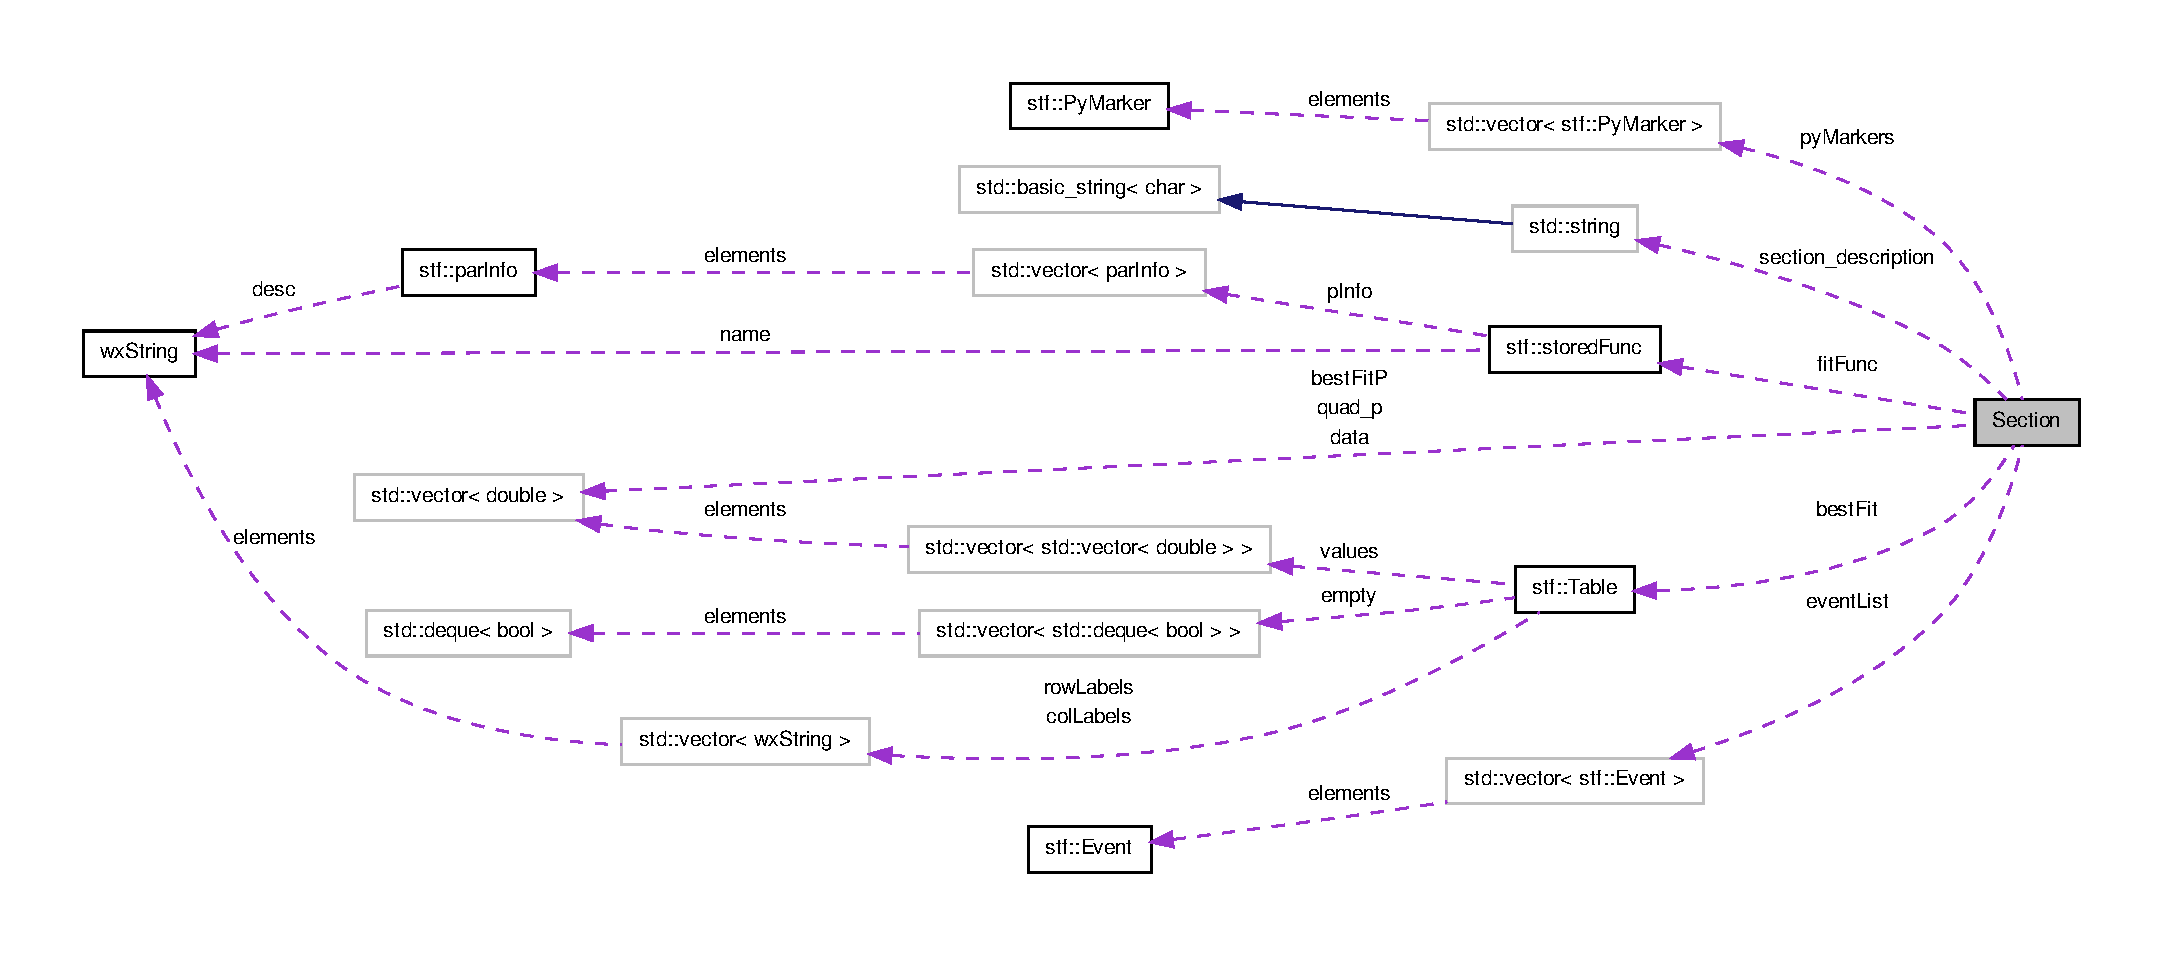
\includegraphics[width=400pt]{classSection__coll__graph}
\end{center}
\end{figure}
\subsection*{Public Member Functions}
\begin{DoxyCompactItemize}
\item 
\hypertarget{classSection_a77b88e06692841ba49559d22a25a09f9}{
\hyperlink{classSection_a77b88e06692841ba49559d22a25a09f9}{Section} ()}
\label{classSection_a77b88e06692841ba49559d22a25a09f9}

\begin{DoxyCompactList}\small\item\em Default constructor. \item\end{DoxyCompactList}\item 
\hyperlink{classSection_ab2a565295bdf8ebb07663aa3442b8957}{Section} (const Vector\_\-double \&valA, const std::string \&label=\char`\"{}$\backslash$0\char`\"{})
\begin{DoxyCompactList}\small\item\em Constructor. \item\end{DoxyCompactList}\item 
\hyperlink{classSection_a8228979f357bdfeeb7ebb91b5c1d1a2c}{Section} (std::size\_\-t size, const std::string \&label=\char`\"{}$\backslash$0\char`\"{})
\begin{DoxyCompactList}\small\item\em Yet another constructor. \item\end{DoxyCompactList}\item 
\hypertarget{classSection_ae2582a77c7ecb8cbd4a1b58e7ad3296e}{
\hyperlink{classSection_ae2582a77c7ecb8cbd4a1b58e7ad3296e}{$\sim$Section} ()}
\label{classSection_ae2582a77c7ecb8cbd4a1b58e7ad3296e}

\begin{DoxyCompactList}\small\item\em Destructor. \item\end{DoxyCompactList}\item 
double \& \hyperlink{classSection_a6f6e72115cb253df1316c2005156fd29}{operator\mbox{[}$\,$\mbox{]}} (std::size\_\-t at)
\begin{DoxyCompactList}\small\item\em Unchecked access. Returns a non-\/const reference. \item\end{DoxyCompactList}\item 
double \hyperlink{classSection_a721b8cf4b65cd5a80f4ad3bb28a24b65}{operator\mbox{[}$\,$\mbox{]}} (std::size\_\-t at) const 
\begin{DoxyCompactList}\small\item\em Unchecked access. Returns a copy. \item\end{DoxyCompactList}\item 
double \hyperlink{classSection_ab98c2b404571d18fe6d48ae2284fe858}{at} (std::size\_\-t at\_\-) const 
\begin{DoxyCompactList}\small\item\em Range-\/checked access. Returns a copy. \item\end{DoxyCompactList}\item 
double \& \hyperlink{classSection_a5b506d0c6ec0fe3ad938198748f6f9c9}{at} (std::size\_\-t at\_\-)
\begin{DoxyCompactList}\small\item\em Range-\/checked access. Returns a non-\/const reference. \item\end{DoxyCompactList}\item 
const Vector\_\-double \& \hyperlink{classSection_ac807068714bffde739c88ab9fde0606a}{get} () const 
\begin{DoxyCompactList}\small\item\em Low-\/level access to the valarray (read-\/only). \item\end{DoxyCompactList}\item 
Vector\_\-double \& \hyperlink{classSection_acdd69b0abf2d2ffd9c85cf3736437c28}{get\_\-w} ()
\begin{DoxyCompactList}\small\item\em Low-\/level access to the valarray (read and write). \item\end{DoxyCompactList}\item 
void \hyperlink{classSection_a6c1d862be679b440e8e5c4536321ad63}{resize} (std::size\_\-t new\_\-size)
\begin{DoxyCompactList}\small\item\em Resize the \hyperlink{classSection}{Section} to a new number of data points; deletes all previously stored data when gcc is used. \item\end{DoxyCompactList}\item 
size\_\-t \hyperlink{classSection_a2bbdfd756c4a51191944b6acb4e730c6}{size} () const 
\begin{DoxyCompactList}\small\item\em Retrieve the number of data points. \item\end{DoxyCompactList}\item 
void \hyperlink{classSection_a2fd59487e56778a833548e68150d1d76}{SetXScale} (double value)
\begin{DoxyCompactList}\small\item\em Sets the x scaling. \item\end{DoxyCompactList}\item 
double \hyperlink{classSection_abefdeba1385a91ed8d151df70deacd00}{GetXScale} () const 
\begin{DoxyCompactList}\small\item\em Retrieves the x scaling. \item\end{DoxyCompactList}\item 
const std::string \& \hyperlink{classSection_a5ca59050bebcc8fb05ae4aa8b795c0c5}{GetSectionDescription} () const 
\begin{DoxyCompactList}\small\item\em Retrieves a section description. \item\end{DoxyCompactList}\item 
void \hyperlink{classSection_a187071317155567ebbb249de9657aca3}{SetSectionDescription} (const std::string \&value)
\begin{DoxyCompactList}\small\item\em Sets a section description. \item\end{DoxyCompactList}\item 
const \hyperlink{structstf_1_1storedFunc}{stf::storedFunc} $\ast$ \hyperlink{classSection_ad4867f096b0fa9bcbfd1793bb002a1b9}{GetFitFunc} () const 
\begin{DoxyCompactList}\small\item\em Retrieves a waveform of the evaluated best-\/fit function (read-\/only) \item\end{DoxyCompactList}\item 
bool \hyperlink{classSection_a333306824e7d67daae711f9cfda5db1d}{IsFitted} () const 
\begin{DoxyCompactList}\small\item\em Indicates whether a fit has been performed on this section. \item\end{DoxyCompactList}\item 
\hypertarget{classSection_af0ed8295201e0b28a90545d315e1c362}{
void \hyperlink{classSection_af0ed8295201e0b28a90545d315e1c362}{DeleteFit} ()}
\label{classSection_af0ed8295201e0b28a90545d315e1c362}

\begin{DoxyCompactList}\small\item\em Deletes the current fit, sete isFitted to false;. \item\end{DoxyCompactList}\item 
void \hyperlink{classSection_a29a599defe60ea0389148978419cc6f0}{SetIsFitted} (const Vector\_\-double \&bestFitP\_\-, \hyperlink{structstf_1_1storedFunc}{stf::storedFunc} $\ast$fitFunc\_\-, double chisqr, std::size\_\-t fitBeg, std::size\_\-t fitEnd)
\begin{DoxyCompactList}\small\item\em Sets the best-\/fit parameters when a fit has been performed on this section. \item\end{DoxyCompactList}\item 
const Vector\_\-double \& \hyperlink{classSection_adba74fc36543f90d9a4441f1dd2fe544}{GetQuadP} () const 
\begin{DoxyCompactList}\small\item\em Retrieves the parameters of quadratic functions, each going through three consecutive data points. \item\end{DoxyCompactList}\item 
const Vector\_\-double \& \hyperlink{classSection_ac42014aaa369eb14375f5a2ae1d85696}{GetBestFitP} () const 
\begin{DoxyCompactList}\small\item\em Retrieves the best-\/fit parameters for the most recently performed fit. \item\end{DoxyCompactList}\item 
bool \hyperlink{classSection_a48cd4ca1fc664cbbee27bdaf9d7e1899}{IsIntegrated} () const 
\begin{DoxyCompactList}\small\item\em Indicates whether an integral has been calculated in this section. \item\end{DoxyCompactList}\item 
void \hyperlink{classSection_a8e69591a80dc21c7ecba523ae15eec3d}{SetIsIntegrated} (bool value=true, std::size\_\-t begin=0, std::size\_\-t end=0)
\begin{DoxyCompactList}\small\item\em Determines whether an integral has been calculated in this section. \item\end{DoxyCompactList}\item 
std::size\_\-t \hyperlink{classSection_a47a32db6afcdbc4a2e0f95d1f0e105cd}{GetStoreFitBeg} () const 
\begin{DoxyCompactList}\small\item\em Retrieves the position of a stored fit start cursor. \item\end{DoxyCompactList}\item 
std::size\_\-t \hyperlink{classSection_aaba1dbe7d8e1cd59f58358c77d81ff6e}{GetStoreFitEnd} () const 
\begin{DoxyCompactList}\small\item\em Retrieves the position of a stored fit end cursor. \item\end{DoxyCompactList}\item 
std::size\_\-t \hyperlink{classSection_a37c7ecd4475a602a94e21278a914244f}{GetStoreIntBeg} () const 
\begin{DoxyCompactList}\small\item\em Retrieves the position of a stored integral start cursor. \item\end{DoxyCompactList}\item 
std::size\_\-t \hyperlink{classSection_a4f694c6afc8423881230cafc2c336187}{GetStoreIntEnd} () const 
\begin{DoxyCompactList}\small\item\em Retrieves the position of a stored integral end cursor. \item\end{DoxyCompactList}\item 
void \hyperlink{classSection_a9b966152b6ec99ad02386505fddbe346}{SetStoreIntBeg} (std::size\_\-t value)
\begin{DoxyCompactList}\small\item\em Stores the position of an integral start cursor. \item\end{DoxyCompactList}\item 
void \hyperlink{classSection_a91ab67845b83473330f5a823e65da511}{SetStoreIntEnd} (std::size\_\-t value)
\begin{DoxyCompactList}\small\item\em Stores the position of an integral end cursor. \item\end{DoxyCompactList}\item 
const \hyperlink{classstf_1_1Table}{stf::Table} \& \hyperlink{classSection_a8a72a7c76100aba788e03e5e2bb1492d}{GetBestFit} () const 
\begin{DoxyCompactList}\small\item\em Retrieves imformation about the last fit that has been performed (read-\/only). \item\end{DoxyCompactList}\item 
const \hyperlink{classstf_1_1Event}{stf::Event} \& \hyperlink{classSection_ad048175b4fcce50838ab5604f435b1f9}{GetEvent} (std::size\_\-t n\_\-e) const 
\begin{DoxyCompactList}\small\item\em Retrieves information about an event. \item\end{DoxyCompactList}\item 
void \hyperlink{classSection_aabad035dd62df6b845bca4138c0685ed}{CreateEvent} (const \hyperlink{classstf_1_1Event}{stf::Event} \&event)
\begin{DoxyCompactList}\small\item\em Creates a new event. \item\end{DoxyCompactList}\item 
bool \hyperlink{classSection_ae9305686a770854b262d8aa75d3398cf}{HasEvents} () const 
\begin{DoxyCompactList}\small\item\em Checks whether any events have been created yet. \item\end{DoxyCompactList}\item 
const std::vector$<$ \hyperlink{classstf_1_1Event}{stf::Event} $>$ \& \hyperlink{classSection_ab1e4f735f699678dca948360fc8f8b51}{GetEvents} () const 
\begin{DoxyCompactList}\small\item\em Retrieves a list with information about events (read-\/only). \item\end{DoxyCompactList}\item 
std::vector$<$ \hyperlink{classstf_1_1Event}{stf::Event} $>$ \& \hyperlink{classSection_a46a0af45a6c08ee391efae80dcd8b663}{GetEventsW} ()
\begin{DoxyCompactList}\small\item\em Retrieves a list with information about events (read and write). \item\end{DoxyCompactList}\item 
\hypertarget{classSection_a7bf02bc096fa3a159cf9e48ac53b48d0}{
void \hyperlink{classSection_a7bf02bc096fa3a159cf9e48ac53b48d0}{EraseEvents} ()}
\label{classSection_a7bf02bc096fa3a159cf9e48ac53b48d0}

\begin{DoxyCompactList}\small\item\em Erases all events. \item\end{DoxyCompactList}\item 
const \hyperlink{structstf_1_1PyMarker}{stf::PyMarker} \& \hyperlink{classSection_a6973cb8f0221bcf14c1340d250a65b8d}{GetPyMarker} (std::size\_\-t n\_\-e) const 
\begin{DoxyCompactList}\small\item\em Retrieves the position of a marker. \item\end{DoxyCompactList}\item 
void \hyperlink{classSection_a46c0073052679f46ce54da0a3a3fce21}{SetPyMarker} (const \hyperlink{structstf_1_1PyMarker}{stf::PyMarker} \&marker)
\begin{DoxyCompactList}\small\item\em Sets a new marker. \item\end{DoxyCompactList}\item 
bool \hyperlink{classSection_ad774d7ea6f7b5c5db422b61aaee9c755}{HasPyMarkers} () const 
\begin{DoxyCompactList}\small\item\em Checks whether any marker has been set yet. \item\end{DoxyCompactList}\item 
const std::vector$<$ \hyperlink{structstf_1_1PyMarker}{stf::PyMarker} $>$ \& \hyperlink{classSection_a9f049021e522755e1eb72b723e71a1f5}{GetPyMarkers} () const 
\begin{DoxyCompactList}\small\item\em Retrieves a list with information about markers (read-\/only). \item\end{DoxyCompactList}\item 
\hypertarget{classSection_a296b4013f761b937d0ca47ab8c5da207}{
void \hyperlink{classSection_a296b4013f761b937d0ca47ab8c5da207}{ErasePyMarkers} ()}
\label{classSection_a296b4013f761b937d0ca47ab8c5da207}

\begin{DoxyCompactList}\small\item\em Erases all events. \item\end{DoxyCompactList}\end{DoxyCompactItemize}


\subsection{Detailed Description}
Represents a continuously sampled sweep of data points. 

\subsection{Constructor \& Destructor Documentation}
\hypertarget{classSection_ab2a565295bdf8ebb07663aa3442b8957}{
\index{Section@{Section}!Section@{Section}}
\index{Section@{Section}!Section@{Section}}
\subsubsection[{Section}]{\setlength{\rightskip}{0pt plus 5cm}Section::Section (
\begin{DoxyParamCaption}
\item[{const Vector\_\-double \&}]{valA, }
\item[{const std::string \&}]{label = {\ttfamily \char`\"{}$\backslash$0\char`\"{}}}
\end{DoxyParamCaption}
)\hspace{0.3cm}{\ttfamily  \mbox{[}explicit\mbox{]}}}}
\label{classSection_ab2a565295bdf8ebb07663aa3442b8957}


Constructor. 


\begin{DoxyParams}{Parameters}
{\em valA} & A vector of values that will make up the section. \\
\hline
{\em label} & An optional section label string. \\
\hline
\end{DoxyParams}
\hypertarget{classSection_a8228979f357bdfeeb7ebb91b5c1d1a2c}{
\index{Section@{Section}!Section@{Section}}
\index{Section@{Section}!Section@{Section}}
\subsubsection[{Section}]{\setlength{\rightskip}{0pt plus 5cm}Section::Section (
\begin{DoxyParamCaption}
\item[{std::size\_\-t}]{size, }
\item[{const std::string \&}]{label = {\ttfamily \char`\"{}$\backslash$0\char`\"{}}}
\end{DoxyParamCaption}
)\hspace{0.3cm}{\ttfamily  \mbox{[}explicit\mbox{]}}}}
\label{classSection_a8228979f357bdfeeb7ebb91b5c1d1a2c}


Yet another constructor. 


\begin{DoxyParams}{Parameters}
{\em size} & Number of data points. \\
\hline
{\em label} & An optional section label string. \\
\hline
\end{DoxyParams}


\subsection{Member Function Documentation}
\hypertarget{classSection_ab98c2b404571d18fe6d48ae2284fe858}{
\index{Section@{Section}!at@{at}}
\index{at@{at}!Section@{Section}}
\subsubsection[{at}]{\setlength{\rightskip}{0pt plus 5cm}double Section::at (
\begin{DoxyParamCaption}
\item[{std::size\_\-t}]{at\_\-}
\end{DoxyParamCaption}
) const}}
\label{classSection_ab98c2b404571d18fe6d48ae2284fe858}


Range-\/checked access. Returns a copy. 

Throws std::out\_\-of\_\-range if out of range. 
\begin{DoxyParams}{Parameters}
{\em at\_\-} & Data point index. \\
\hline
\end{DoxyParams}
\begin{DoxyReturn}{Returns}
Copy of the data point at index at\_\- 
\end{DoxyReturn}
\hypertarget{classSection_a5b506d0c6ec0fe3ad938198748f6f9c9}{
\index{Section@{Section}!at@{at}}
\index{at@{at}!Section@{Section}}
\subsubsection[{at}]{\setlength{\rightskip}{0pt plus 5cm}double\& Section::at (
\begin{DoxyParamCaption}
\item[{std::size\_\-t}]{at\_\-}
\end{DoxyParamCaption}
)}}
\label{classSection_a5b506d0c6ec0fe3ad938198748f6f9c9}


Range-\/checked access. Returns a non-\/const reference. 

Throws std::out\_\-of\_\-range if out of range. 
\begin{DoxyParams}{Parameters}
{\em at\_\-} & Data point index. \\
\hline
\end{DoxyParams}
\begin{DoxyReturn}{Returns}
Reference to the data point at index at\_\- 
\end{DoxyReturn}
\hypertarget{classSection_aabad035dd62df6b845bca4138c0685ed}{
\index{Section@{Section}!CreateEvent@{CreateEvent}}
\index{CreateEvent@{CreateEvent}!Section@{Section}}
\subsubsection[{CreateEvent}]{\setlength{\rightskip}{0pt plus 5cm}void Section::CreateEvent (
\begin{DoxyParamCaption}
\item[{const {\bf stf::Event} \&}]{event}
\end{DoxyParamCaption}
)\hspace{0.3cm}{\ttfamily  \mbox{[}inline\mbox{]}}}}
\label{classSection_aabad035dd62df6b845bca4138c0685ed}


Creates a new event. 


\begin{DoxyParams}{Parameters}
{\em event} & Information about the event. \\
\hline
\end{DoxyParams}
\hypertarget{classSection_ac807068714bffde739c88ab9fde0606a}{
\index{Section@{Section}!get@{get}}
\index{get@{get}!Section@{Section}}
\subsubsection[{get}]{\setlength{\rightskip}{0pt plus 5cm}const Vector\_\-double\& Section::get (
\begin{DoxyParamCaption}
{}
\end{DoxyParamCaption}
) const\hspace{0.3cm}{\ttfamily  \mbox{[}inline\mbox{]}}}}
\label{classSection_ac807068714bffde739c88ab9fde0606a}


Low-\/level access to the valarray (read-\/only). 

An explicit function is used instead of implicit type conversion to access the valarray. \begin{DoxyReturn}{Returns}
The valarray containing the data points. 
\end{DoxyReturn}
\hypertarget{classSection_acdd69b0abf2d2ffd9c85cf3736437c28}{
\index{Section@{Section}!get\_\-w@{get\_\-w}}
\index{get\_\-w@{get\_\-w}!Section@{Section}}
\subsubsection[{get\_\-w}]{\setlength{\rightskip}{0pt plus 5cm}Vector\_\-double\& Section::get\_\-w (
\begin{DoxyParamCaption}
{}
\end{DoxyParamCaption}
)\hspace{0.3cm}{\ttfamily  \mbox{[}inline\mbox{]}}}}
\label{classSection_acdd69b0abf2d2ffd9c85cf3736437c28}


Low-\/level access to the valarray (read and write). 

An explicit function is used instead of implicit type conversion to access the valarray. \begin{DoxyReturn}{Returns}
The valarray containing the data points. 
\end{DoxyReturn}
\hypertarget{classSection_a8a72a7c76100aba788e03e5e2bb1492d}{
\index{Section@{Section}!GetBestFit@{GetBestFit}}
\index{GetBestFit@{GetBestFit}!Section@{Section}}
\subsubsection[{GetBestFit}]{\setlength{\rightskip}{0pt plus 5cm}const {\bf stf::Table}\& Section::GetBestFit (
\begin{DoxyParamCaption}
{}
\end{DoxyParamCaption}
) const\hspace{0.3cm}{\ttfamily  \mbox{[}inline\mbox{]}}}}
\label{classSection_a8a72a7c76100aba788e03e5e2bb1492d}


Retrieves imformation about the last fit that has been performed (read-\/only). 

\begin{DoxyReturn}{Returns}
A table with information about the last fit. 
\end{DoxyReturn}
\hypertarget{classSection_ac42014aaa369eb14375f5a2ae1d85696}{
\index{Section@{Section}!GetBestFitP@{GetBestFitP}}
\index{GetBestFitP@{GetBestFitP}!Section@{Section}}
\subsubsection[{GetBestFitP}]{\setlength{\rightskip}{0pt plus 5cm}const Vector\_\-double\& Section::GetBestFitP (
\begin{DoxyParamCaption}
{}
\end{DoxyParamCaption}
) const\hspace{0.3cm}{\ttfamily  \mbox{[}inline\mbox{]}}}}
\label{classSection_ac42014aaa369eb14375f5a2ae1d85696}


Retrieves the best-\/fit parameters for the most recently performed fit. 

\begin{DoxyReturn}{Returns}
A std::vector of best-\/fit parameters. 
\end{DoxyReturn}
\hypertarget{classSection_ad048175b4fcce50838ab5604f435b1f9}{
\index{Section@{Section}!GetEvent@{GetEvent}}
\index{GetEvent@{GetEvent}!Section@{Section}}
\subsubsection[{GetEvent}]{\setlength{\rightskip}{0pt plus 5cm}const {\bf stf::Event}\& Section::GetEvent (
\begin{DoxyParamCaption}
\item[{std::size\_\-t}]{n\_\-e}
\end{DoxyParamCaption}
) const}}
\label{classSection_ad048175b4fcce50838ab5604f435b1f9}


Retrieves information about an event. 


\begin{DoxyParams}{Parameters}
{\em n\_\-e} & The index of the event. \\
\hline
\end{DoxyParams}
\begin{DoxyReturn}{Returns}
An Event object containing information about an event. 
\end{DoxyReturn}
\hypertarget{classSection_ab1e4f735f699678dca948360fc8f8b51}{
\index{Section@{Section}!GetEvents@{GetEvents}}
\index{GetEvents@{GetEvents}!Section@{Section}}
\subsubsection[{GetEvents}]{\setlength{\rightskip}{0pt plus 5cm}const std::vector$<${\bf stf::Event}$>$\& Section::GetEvents (
\begin{DoxyParamCaption}
{}
\end{DoxyParamCaption}
) const\hspace{0.3cm}{\ttfamily  \mbox{[}inline\mbox{]}}}}
\label{classSection_ab1e4f735f699678dca948360fc8f8b51}


Retrieves a list with information about events (read-\/only). 

\begin{DoxyReturn}{Returns}
A vector with event information. 
\end{DoxyReturn}
\hypertarget{classSection_a46a0af45a6c08ee391efae80dcd8b663}{
\index{Section@{Section}!GetEventsW@{GetEventsW}}
\index{GetEventsW@{GetEventsW}!Section@{Section}}
\subsubsection[{GetEventsW}]{\setlength{\rightskip}{0pt plus 5cm}std::vector$<${\bf stf::Event}$>$\& Section::GetEventsW (
\begin{DoxyParamCaption}
{}
\end{DoxyParamCaption}
)\hspace{0.3cm}{\ttfamily  \mbox{[}inline\mbox{]}}}}
\label{classSection_a46a0af45a6c08ee391efae80dcd8b663}


Retrieves a list with information about events (read and write). 

\begin{DoxyReturn}{Returns}
A vector with event information. 
\end{DoxyReturn}
\hypertarget{classSection_ad4867f096b0fa9bcbfd1793bb002a1b9}{
\index{Section@{Section}!GetFitFunc@{GetFitFunc}}
\index{GetFitFunc@{GetFitFunc}!Section@{Section}}
\subsubsection[{GetFitFunc}]{\setlength{\rightskip}{0pt plus 5cm}const {\bf stf::storedFunc}$\ast$ Section::GetFitFunc (
\begin{DoxyParamCaption}
{}
\end{DoxyParamCaption}
) const\hspace{0.3cm}{\ttfamily  \mbox{[}inline\mbox{]}}}}
\label{classSection_ad4867f096b0fa9bcbfd1793bb002a1b9}


Retrieves a waveform of the evaluated best-\/fit function (read-\/only) 

\begin{DoxyReturn}{Returns}
A valarray containing the evaluated best-\/fit function. 
\end{DoxyReturn}
\hypertarget{classSection_a6973cb8f0221bcf14c1340d250a65b8d}{
\index{Section@{Section}!GetPyMarker@{GetPyMarker}}
\index{GetPyMarker@{GetPyMarker}!Section@{Section}}
\subsubsection[{GetPyMarker}]{\setlength{\rightskip}{0pt plus 5cm}const {\bf stf::PyMarker}\& Section::GetPyMarker (
\begin{DoxyParamCaption}
\item[{std::size\_\-t}]{n\_\-e}
\end{DoxyParamCaption}
) const}}
\label{classSection_a6973cb8f0221bcf14c1340d250a65b8d}


Retrieves the position of a marker. 


\begin{DoxyParams}{Parameters}
{\em n\_\-e} & The index of the marker. \\
\hline
\end{DoxyParams}
\begin{DoxyReturn}{Returns}
The marker (a pair of x,y coordinates) 
\end{DoxyReturn}
\hypertarget{classSection_a9f049021e522755e1eb72b723e71a1f5}{
\index{Section@{Section}!GetPyMarkers@{GetPyMarkers}}
\index{GetPyMarkers@{GetPyMarkers}!Section@{Section}}
\subsubsection[{GetPyMarkers}]{\setlength{\rightskip}{0pt plus 5cm}const std::vector$<${\bf stf::PyMarker}$>$\& Section::GetPyMarkers (
\begin{DoxyParamCaption}
{}
\end{DoxyParamCaption}
) const\hspace{0.3cm}{\ttfamily  \mbox{[}inline\mbox{]}}}}
\label{classSection_a9f049021e522755e1eb72b723e71a1f5}


Retrieves a list with information about markers (read-\/only). 

\begin{DoxyReturn}{Returns}
A vector with markers. 
\end{DoxyReturn}
\hypertarget{classSection_adba74fc36543f90d9a4441f1dd2fe544}{
\index{Section@{Section}!GetQuadP@{GetQuadP}}
\index{GetQuadP@{GetQuadP}!Section@{Section}}
\subsubsection[{GetQuadP}]{\setlength{\rightskip}{0pt plus 5cm}const Vector\_\-double\& Section::GetQuadP (
\begin{DoxyParamCaption}
{}
\end{DoxyParamCaption}
) const\hspace{0.3cm}{\ttfamily  \mbox{[}inline\mbox{]}}}}
\label{classSection_adba74fc36543f90d9a4441f1dd2fe544}


Retrieves the parameters of quadratic functions, each going through three consecutive data points. 

\begin{DoxyReturn}{Returns}
Parameters of quadratic functions of the form a0$\ast$x$^\wedge$2 + b0$\ast$x + c0, a1$\ast$x$^\wedge$2 + b1$\ast$x + c1, ..., an$\ast$x$^\wedge$2 + bn$\ast$x + cn Each quadratic function goes through three consecutive data points. 
\end{DoxyReturn}
\hypertarget{classSection_a5ca59050bebcc8fb05ae4aa8b795c0c5}{
\index{Section@{Section}!GetSectionDescription@{GetSectionDescription}}
\index{GetSectionDescription@{GetSectionDescription}!Section@{Section}}
\subsubsection[{GetSectionDescription}]{\setlength{\rightskip}{0pt plus 5cm}const std::string\& Section::GetSectionDescription (
\begin{DoxyParamCaption}
{}
\end{DoxyParamCaption}
) const\hspace{0.3cm}{\ttfamily  \mbox{[}inline\mbox{]}}}}
\label{classSection_a5ca59050bebcc8fb05ae4aa8b795c0c5}


Retrieves a section description. 

\begin{DoxyReturn}{Returns}
A string describing this section. 
\end{DoxyReturn}
\hypertarget{classSection_a47a32db6afcdbc4a2e0f95d1f0e105cd}{
\index{Section@{Section}!GetStoreFitBeg@{GetStoreFitBeg}}
\index{GetStoreFitBeg@{GetStoreFitBeg}!Section@{Section}}
\subsubsection[{GetStoreFitBeg}]{\setlength{\rightskip}{0pt plus 5cm}std::size\_\-t Section::GetStoreFitBeg (
\begin{DoxyParamCaption}
{}
\end{DoxyParamCaption}
) const\hspace{0.3cm}{\ttfamily  \mbox{[}inline\mbox{]}}}}
\label{classSection_a47a32db6afcdbc4a2e0f95d1f0e105cd}


Retrieves the position of a stored fit start cursor. 

Note that cursors are usually managed in \hyperlink{classRecording}{Recording}. However, the fit cursors are stored here so that a previous fit can be restored when this section is activated again. \begin{DoxyReturn}{Returns}
Fit start cursor position from a previous fit. 
\end{DoxyReturn}
\hypertarget{classSection_aaba1dbe7d8e1cd59f58358c77d81ff6e}{
\index{Section@{Section}!GetStoreFitEnd@{GetStoreFitEnd}}
\index{GetStoreFitEnd@{GetStoreFitEnd}!Section@{Section}}
\subsubsection[{GetStoreFitEnd}]{\setlength{\rightskip}{0pt plus 5cm}std::size\_\-t Section::GetStoreFitEnd (
\begin{DoxyParamCaption}
{}
\end{DoxyParamCaption}
) const\hspace{0.3cm}{\ttfamily  \mbox{[}inline\mbox{]}}}}
\label{classSection_aaba1dbe7d8e1cd59f58358c77d81ff6e}


Retrieves the position of a stored fit end cursor. 

Note that cursors are usually managed in \hyperlink{classRecording}{Recording}. However, the fit cursors are stored here so that a previous fit can be restored when this section is activated again. \begin{DoxyReturn}{Returns}
Fit end cursor position from a previous fit. 
\end{DoxyReturn}
\hypertarget{classSection_a37c7ecd4475a602a94e21278a914244f}{
\index{Section@{Section}!GetStoreIntBeg@{GetStoreIntBeg}}
\index{GetStoreIntBeg@{GetStoreIntBeg}!Section@{Section}}
\subsubsection[{GetStoreIntBeg}]{\setlength{\rightskip}{0pt plus 5cm}std::size\_\-t Section::GetStoreIntBeg (
\begin{DoxyParamCaption}
{}
\end{DoxyParamCaption}
) const\hspace{0.3cm}{\ttfamily  \mbox{[}inline\mbox{]}}}}
\label{classSection_a37c7ecd4475a602a94e21278a914244f}


Retrieves the position of a stored integral start cursor. 

Note that cursors are usually managed in \hyperlink{classRecording}{Recording}. However, the integral cursors are stored here so that a previous integral can be restored when this section is activated again. \begin{DoxyReturn}{Returns}
Integral start cursor position from a previous integral calculation. 
\end{DoxyReturn}
\hypertarget{classSection_a4f694c6afc8423881230cafc2c336187}{
\index{Section@{Section}!GetStoreIntEnd@{GetStoreIntEnd}}
\index{GetStoreIntEnd@{GetStoreIntEnd}!Section@{Section}}
\subsubsection[{GetStoreIntEnd}]{\setlength{\rightskip}{0pt plus 5cm}std::size\_\-t Section::GetStoreIntEnd (
\begin{DoxyParamCaption}
{}
\end{DoxyParamCaption}
) const\hspace{0.3cm}{\ttfamily  \mbox{[}inline\mbox{]}}}}
\label{classSection_a4f694c6afc8423881230cafc2c336187}


Retrieves the position of a stored integral end cursor. 

Note that cursors are usually managed in \hyperlink{classRecording}{Recording}. However, the integral cursors are stored here so that a previous integral can be restored when this section is activated again. \begin{DoxyReturn}{Returns}
Integral end cursor position from a previous integral calculation. 
\end{DoxyReturn}
\hypertarget{classSection_abefdeba1385a91ed8d151df70deacd00}{
\index{Section@{Section}!GetXScale@{GetXScale}}
\index{GetXScale@{GetXScale}!Section@{Section}}
\subsubsection[{GetXScale}]{\setlength{\rightskip}{0pt plus 5cm}double Section::GetXScale (
\begin{DoxyParamCaption}
{}
\end{DoxyParamCaption}
) const\hspace{0.3cm}{\ttfamily  \mbox{[}inline\mbox{]}}}}
\label{classSection_abefdeba1385a91ed8d151df70deacd00}


Retrieves the x scaling. 

\begin{DoxyReturn}{Returns}
The x scaling. 
\end{DoxyReturn}
\hypertarget{classSection_ae9305686a770854b262d8aa75d3398cf}{
\index{Section@{Section}!HasEvents@{HasEvents}}
\index{HasEvents@{HasEvents}!Section@{Section}}
\subsubsection[{HasEvents}]{\setlength{\rightskip}{0pt plus 5cm}bool Section::HasEvents (
\begin{DoxyParamCaption}
{}
\end{DoxyParamCaption}
) const\hspace{0.3cm}{\ttfamily  \mbox{[}inline\mbox{]}}}}
\label{classSection_ae9305686a770854b262d8aa75d3398cf}


Checks whether any events have been created yet. 

\begin{DoxyReturn}{Returns}
true if there are any events, false otherwise. 
\end{DoxyReturn}
\hypertarget{classSection_ad774d7ea6f7b5c5db422b61aaee9c755}{
\index{Section@{Section}!HasPyMarkers@{HasPyMarkers}}
\index{HasPyMarkers@{HasPyMarkers}!Section@{Section}}
\subsubsection[{HasPyMarkers}]{\setlength{\rightskip}{0pt plus 5cm}bool Section::HasPyMarkers (
\begin{DoxyParamCaption}
{}
\end{DoxyParamCaption}
) const\hspace{0.3cm}{\ttfamily  \mbox{[}inline\mbox{]}}}}
\label{classSection_ad774d7ea6f7b5c5db422b61aaee9c755}


Checks whether any marker has been set yet. 

\begin{DoxyReturn}{Returns}
true if there are any markers, false otherwise. 
\end{DoxyReturn}
\hypertarget{classSection_a333306824e7d67daae711f9cfda5db1d}{
\index{Section@{Section}!IsFitted@{IsFitted}}
\index{IsFitted@{IsFitted}!Section@{Section}}
\subsubsection[{IsFitted}]{\setlength{\rightskip}{0pt plus 5cm}bool Section::IsFitted (
\begin{DoxyParamCaption}
{}
\end{DoxyParamCaption}
) const\hspace{0.3cm}{\ttfamily  \mbox{[}inline\mbox{]}}}}
\label{classSection_a333306824e7d67daae711f9cfda5db1d}


Indicates whether a fit has been performed on this section. 

\begin{DoxyReturn}{Returns}
true if a fit has been performed, false otherwise. 
\end{DoxyReturn}
\hypertarget{classSection_a48cd4ca1fc664cbbee27bdaf9d7e1899}{
\index{Section@{Section}!IsIntegrated@{IsIntegrated}}
\index{IsIntegrated@{IsIntegrated}!Section@{Section}}
\subsubsection[{IsIntegrated}]{\setlength{\rightskip}{0pt plus 5cm}bool Section::IsIntegrated (
\begin{DoxyParamCaption}
{}
\end{DoxyParamCaption}
) const\hspace{0.3cm}{\ttfamily  \mbox{[}inline\mbox{]}}}}
\label{classSection_a48cd4ca1fc664cbbee27bdaf9d7e1899}


Indicates whether an integral has been calculated in this section. 

\begin{DoxyReturn}{Returns}
true if an integral has been calculated, false otherwise. 
\end{DoxyReturn}
\hypertarget{classSection_a721b8cf4b65cd5a80f4ad3bb28a24b65}{
\index{Section@{Section}!operator\mbox{[}\mbox{]}@{operator[]}}
\index{operator\mbox{[}\mbox{]}@{operator[]}!Section@{Section}}
\subsubsection[{operator[]}]{\setlength{\rightskip}{0pt plus 5cm}double Section::operator\mbox{[}$\,$\mbox{]} (
\begin{DoxyParamCaption}
\item[{std::size\_\-t}]{at}
\end{DoxyParamCaption}
) const\hspace{0.3cm}{\ttfamily  \mbox{[}inline\mbox{]}}}}
\label{classSection_a721b8cf4b65cd5a80f4ad3bb28a24b65}


Unchecked access. Returns a copy. 


\begin{DoxyParams}{Parameters}
{\em at} & Data point index. \\
\hline
\end{DoxyParams}
\begin{DoxyReturn}{Returns}
Reference to the data point with index at. 
\end{DoxyReturn}
\hypertarget{classSection_a6f6e72115cb253df1316c2005156fd29}{
\index{Section@{Section}!operator\mbox{[}\mbox{]}@{operator[]}}
\index{operator\mbox{[}\mbox{]}@{operator[]}!Section@{Section}}
\subsubsection[{operator[]}]{\setlength{\rightskip}{0pt plus 5cm}double\& Section::operator\mbox{[}$\,$\mbox{]} (
\begin{DoxyParamCaption}
\item[{std::size\_\-t}]{at}
\end{DoxyParamCaption}
)\hspace{0.3cm}{\ttfamily  \mbox{[}inline\mbox{]}}}}
\label{classSection_a6f6e72115cb253df1316c2005156fd29}


Unchecked access. Returns a non-\/const reference. 


\begin{DoxyParams}{Parameters}
{\em at} & Data point index. \\
\hline
\end{DoxyParams}
\begin{DoxyReturn}{Returns}
Copy of the data point with index at. 
\end{DoxyReturn}
\hypertarget{classSection_a6c1d862be679b440e8e5c4536321ad63}{
\index{Section@{Section}!resize@{resize}}
\index{resize@{resize}!Section@{Section}}
\subsubsection[{resize}]{\setlength{\rightskip}{0pt plus 5cm}void Section::resize (
\begin{DoxyParamCaption}
\item[{std::size\_\-t}]{new\_\-size}
\end{DoxyParamCaption}
)\hspace{0.3cm}{\ttfamily  \mbox{[}inline\mbox{]}}}}
\label{classSection_a6c1d862be679b440e8e5c4536321ad63}


Resize the \hyperlink{classSection}{Section} to a new number of data points; deletes all previously stored data when gcc is used. 

Note that in the gcc implementation of std::vector, resizing will delete all the original data. This is different from std::vector::resize(). 
\begin{DoxyParams}{Parameters}
{\em new\_\-size} & The new number of data points. \\
\hline
\end{DoxyParams}
\hypertarget{classSection_a29a599defe60ea0389148978419cc6f0}{
\index{Section@{Section}!SetIsFitted@{SetIsFitted}}
\index{SetIsFitted@{SetIsFitted}!Section@{Section}}
\subsubsection[{SetIsFitted}]{\setlength{\rightskip}{0pt plus 5cm}void Section::SetIsFitted (
\begin{DoxyParamCaption}
\item[{const Vector\_\-double \&}]{bestFitP\_\-, }
\item[{{\bf stf::storedFunc} $\ast$}]{fitFunc\_\-, }
\item[{double}]{chisqr, }
\item[{std::size\_\-t}]{fitBeg, }
\item[{std::size\_\-t}]{fitEnd}
\end{DoxyParamCaption}
)}}
\label{classSection_a29a599defe60ea0389148978419cc6f0}


Sets the best-\/fit parameters when a fit has been performed on this section. 


\begin{DoxyParams}{Parameters}
{\em bestFitP\_\-} & The best-\/fit parameters \\
\hline
{\em fitFunc\_\-} & The function used for fitting \\
\hline
{\em chisqr} & The sum of squared errors \\
\hline
{\em fitBeg} & Sampling point index where the fit starts \\
\hline
{\em fitEnd} & Sampling point index where the fit ends \\
\hline
\end{DoxyParams}
\hypertarget{classSection_a8e69591a80dc21c7ecba523ae15eec3d}{
\index{Section@{Section}!SetIsIntegrated@{SetIsIntegrated}}
\index{SetIsIntegrated@{SetIsIntegrated}!Section@{Section}}
\subsubsection[{SetIsIntegrated}]{\setlength{\rightskip}{0pt plus 5cm}void Section::SetIsIntegrated (
\begin{DoxyParamCaption}
\item[{bool}]{value = {\ttfamily true}, }
\item[{std::size\_\-t}]{begin = {\ttfamily 0}, }
\item[{std::size\_\-t}]{end = {\ttfamily 0}}
\end{DoxyParamCaption}
)}}
\label{classSection_a8e69591a80dc21c7ecba523ae15eec3d}


Determines whether an integral has been calculated in this section. 

\begin{DoxyReturn}{Returns}
true if an integral has been calculated, false otherwise. 
\end{DoxyReturn}
\hypertarget{classSection_a46c0073052679f46ce54da0a3a3fce21}{
\index{Section@{Section}!SetPyMarker@{SetPyMarker}}
\index{SetPyMarker@{SetPyMarker}!Section@{Section}}
\subsubsection[{SetPyMarker}]{\setlength{\rightskip}{0pt plus 5cm}void Section::SetPyMarker (
\begin{DoxyParamCaption}
\item[{const {\bf stf::PyMarker} \&}]{marker}
\end{DoxyParamCaption}
)\hspace{0.3cm}{\ttfamily  \mbox{[}inline\mbox{]}}}}
\label{classSection_a46c0073052679f46ce54da0a3a3fce21}


Sets a new marker. 


\begin{DoxyParams}{Parameters}
{\em marker} & The new marker. \\
\hline
\end{DoxyParams}
\hypertarget{classSection_a187071317155567ebbb249de9657aca3}{
\index{Section@{Section}!SetSectionDescription@{SetSectionDescription}}
\index{SetSectionDescription@{SetSectionDescription}!Section@{Section}}
\subsubsection[{SetSectionDescription}]{\setlength{\rightskip}{0pt plus 5cm}void Section::SetSectionDescription (
\begin{DoxyParamCaption}
\item[{const std::string \&}]{value}
\end{DoxyParamCaption}
)\hspace{0.3cm}{\ttfamily  \mbox{[}inline\mbox{]}}}}
\label{classSection_a187071317155567ebbb249de9657aca3}


Sets a section description. 


\begin{DoxyParams}{Parameters}
{\em value} & A string describing this section. \\
\hline
\end{DoxyParams}
\hypertarget{classSection_a9b966152b6ec99ad02386505fddbe346}{
\index{Section@{Section}!SetStoreIntBeg@{SetStoreIntBeg}}
\index{SetStoreIntBeg@{SetStoreIntBeg}!Section@{Section}}
\subsubsection[{SetStoreIntBeg}]{\setlength{\rightskip}{0pt plus 5cm}void Section::SetStoreIntBeg (
\begin{DoxyParamCaption}
\item[{std::size\_\-t}]{value}
\end{DoxyParamCaption}
)\hspace{0.3cm}{\ttfamily  \mbox{[}inline\mbox{]}}}}
\label{classSection_a9b966152b6ec99ad02386505fddbe346}


Stores the position of an integral start cursor. 

Note that cursors are usually managed in \hyperlink{classRecording}{Recording}. However, the integral cursors are stored here so that a previous integral can be restored when this section is activated again. 
\begin{DoxyParams}{Parameters}
{\em value} & Integral start cursor position to be stored. \\
\hline
\end{DoxyParams}
\hypertarget{classSection_a91ab67845b83473330f5a823e65da511}{
\index{Section@{Section}!SetStoreIntEnd@{SetStoreIntEnd}}
\index{SetStoreIntEnd@{SetStoreIntEnd}!Section@{Section}}
\subsubsection[{SetStoreIntEnd}]{\setlength{\rightskip}{0pt plus 5cm}void Section::SetStoreIntEnd (
\begin{DoxyParamCaption}
\item[{std::size\_\-t}]{value}
\end{DoxyParamCaption}
)\hspace{0.3cm}{\ttfamily  \mbox{[}inline\mbox{]}}}}
\label{classSection_a91ab67845b83473330f5a823e65da511}


Stores the position of an integral end cursor. 

Note that cursors are usually managed in \hyperlink{classRecording}{Recording}. However, the integral cursors are stored here so that a previous integral can be restored when this section is activated again. 
\begin{DoxyParams}{Parameters}
{\em value} & Integral end cursor position to be stored. \\
\hline
\end{DoxyParams}
\hypertarget{classSection_a2fd59487e56778a833548e68150d1d76}{
\index{Section@{Section}!SetXScale@{SetXScale}}
\index{SetXScale@{SetXScale}!Section@{Section}}
\subsubsection[{SetXScale}]{\setlength{\rightskip}{0pt plus 5cm}void Section::SetXScale (
\begin{DoxyParamCaption}
\item[{double}]{value}
\end{DoxyParamCaption}
)}}
\label{classSection_a2fd59487e56778a833548e68150d1d76}


Sets the x scaling. 


\begin{DoxyParams}{Parameters}
{\em value} & The x scaling. \\
\hline
\end{DoxyParams}
\hypertarget{classSection_a2bbdfd756c4a51191944b6acb4e730c6}{
\index{Section@{Section}!size@{size}}
\index{size@{size}!Section@{Section}}
\subsubsection[{size}]{\setlength{\rightskip}{0pt plus 5cm}size\_\-t Section::size (
\begin{DoxyParamCaption}
{}
\end{DoxyParamCaption}
) const\hspace{0.3cm}{\ttfamily  \mbox{[}inline\mbox{]}}}}
\label{classSection_a2bbdfd756c4a51191944b6acb4e730c6}


Retrieve the number of data points. 

\begin{DoxyReturn}{Returns}
The number of data points. 
\end{DoxyReturn}


The documentation for this class was generated from the following file:\begin{DoxyCompactItemize}
\item 
src/core/\hyperlink{section_8h}{section.h}\end{DoxyCompactItemize}

\hypertarget{classstf_1_1Event}{
\section{stf::Event Class Reference}
\label{classstf_1_1Event}\index{stf::Event@{stf::Event}}
}


Describes the attributes of an event.  




{\ttfamily \#include $<$stimdefs.h$>$}

\subsection*{Public Member Functions}
\begin{DoxyCompactItemize}
\item 
\hypertarget{classstf_1_1Event_a9f60134377b70dc610c2a49259d9d5f3}{
\hyperlink{classstf_1_1Event_a9f60134377b70dc610c2a49259d9d5f3}{Event} (std::size\_\-t start, std::size\_\-t peak, std::size\_\-t size, bool discard\_\-=false)}
\label{classstf_1_1Event_a9f60134377b70dc610c2a49259d9d5f3}

\begin{DoxyCompactList}\small\item\em Constructor. \item\end{DoxyCompactList}\item 
\hypertarget{classstf_1_1Event_a4665d0e3a410f77f5c61cabebe00ace9}{
\hyperlink{classstf_1_1Event_a4665d0e3a410f77f5c61cabebe00ace9}{$\sim$Event} ()}
\label{classstf_1_1Event_a4665d0e3a410f77f5c61cabebe00ace9}

\begin{DoxyCompactList}\small\item\em Destructor. \item\end{DoxyCompactList}\item 
std::size\_\-t \hyperlink{classstf_1_1Event_a1ed7132d749cc661ac4bbf1d1be066f0}{GetEventStartIndex} () const 
\begin{DoxyCompactList}\small\item\em Retrieves the start index of an event. \item\end{DoxyCompactList}\item 
std::size\_\-t \hyperlink{classstf_1_1Event_adace5488a38346b3420ec6878dbcef27}{GetEventPeakIndex} () const 
\begin{DoxyCompactList}\small\item\em Retrieves the index of an event's peak. \item\end{DoxyCompactList}\item 
std::size\_\-t \hyperlink{classstf_1_1Event_ac2e79cea403141bd2ff4d8578b70eb4a}{GetEventSize} () const 
\begin{DoxyCompactList}\small\item\em Retrieves the size of an event. \item\end{DoxyCompactList}\item 
bool \hyperlink{classstf_1_1Event_a2a31181298f0abaeae1ea38baebe89ef}{GetDiscard} () const 
\begin{DoxyCompactList}\small\item\em Indicates whether an event should be discarded. \item\end{DoxyCompactList}\item 
void \hyperlink{classstf_1_1Event_a751e0e4136119571080c234251420457}{SetEventStartIndex} (std::size\_\-t value)
\begin{DoxyCompactList}\small\item\em Sets the start index of an event. \item\end{DoxyCompactList}\item 
void \hyperlink{classstf_1_1Event_afa8ecb914cc1e72ede33463a8f249ecd}{SetEventPeakIndex} (std::size\_\-t value)
\begin{DoxyCompactList}\small\item\em Sets the index of an event's peak. \item\end{DoxyCompactList}\item 
void \hyperlink{classstf_1_1Event_a9e2803e268c89ae97951836dc89c50aa}{SetEventSize} (std::size\_\-t value)
\begin{DoxyCompactList}\small\item\em Sets the size of an event. \item\end{DoxyCompactList}\item 
void \hyperlink{classstf_1_1Event_a4b6df1bf5749968ca45c42c1c18bb77a}{SetDiscard} (bool value)
\begin{DoxyCompactList}\small\item\em Determines whether an event should be discarded. \item\end{DoxyCompactList}\item 
\hypertarget{classstf_1_1Event_abd78c208b33e6b095dcf1f49bb9eaa92}{
void \hyperlink{classstf_1_1Event_abd78c208b33e6b095dcf1f49bb9eaa92}{ToggleStatus} ()}
\label{classstf_1_1Event_abd78c208b33e6b095dcf1f49bb9eaa92}

\begin{DoxyCompactList}\small\item\em Sets discard to true if it was false and vice versa. \item\end{DoxyCompactList}\end{DoxyCompactItemize}


\subsection{Detailed Description}
Describes the attributes of an event. 

\subsection{Member Function Documentation}
\hypertarget{classstf_1_1Event_a2a31181298f0abaeae1ea38baebe89ef}{
\index{stf::Event@{stf::Event}!GetDiscard@{GetDiscard}}
\index{GetDiscard@{GetDiscard}!stf::Event@{stf::Event}}
\subsubsection[{GetDiscard}]{\setlength{\rightskip}{0pt plus 5cm}bool stf::Event::GetDiscard (
\begin{DoxyParamCaption}
{}
\end{DoxyParamCaption}
) const\hspace{0.3cm}{\ttfamily  \mbox{[}inline\mbox{]}}}}
\label{classstf_1_1Event_a2a31181298f0abaeae1ea38baebe89ef}


Indicates whether an event should be discarded. 

\begin{DoxyReturn}{Returns}
true if it should be discarded, false otherwise. 
\end{DoxyReturn}


Referenced by wxStfCheckBox::ResetEvent().

\hypertarget{classstf_1_1Event_adace5488a38346b3420ec6878dbcef27}{
\index{stf::Event@{stf::Event}!GetEventPeakIndex@{GetEventPeakIndex}}
\index{GetEventPeakIndex@{GetEventPeakIndex}!stf::Event@{stf::Event}}
\subsubsection[{GetEventPeakIndex}]{\setlength{\rightskip}{0pt plus 5cm}std::size\_\-t stf::Event::GetEventPeakIndex (
\begin{DoxyParamCaption}
{}
\end{DoxyParamCaption}
) const\hspace{0.3cm}{\ttfamily  \mbox{[}inline\mbox{]}}}}
\label{classstf_1_1Event_adace5488a38346b3420ec6878dbcef27}


Retrieves the index of an event's peak. 

\begin{DoxyReturn}{Returns}
The index of an event's peak within a section. 
\end{DoxyReturn}
\hypertarget{classstf_1_1Event_ac2e79cea403141bd2ff4d8578b70eb4a}{
\index{stf::Event@{stf::Event}!GetEventSize@{GetEventSize}}
\index{GetEventSize@{GetEventSize}!stf::Event@{stf::Event}}
\subsubsection[{GetEventSize}]{\setlength{\rightskip}{0pt plus 5cm}std::size\_\-t stf::Event::GetEventSize (
\begin{DoxyParamCaption}
{}
\end{DoxyParamCaption}
) const\hspace{0.3cm}{\ttfamily  \mbox{[}inline\mbox{]}}}}
\label{classstf_1_1Event_ac2e79cea403141bd2ff4d8578b70eb4a}


Retrieves the size of an event. 

\begin{DoxyReturn}{Returns}
The size of an event in units of data points. 
\end{DoxyReturn}
\hypertarget{classstf_1_1Event_a1ed7132d749cc661ac4bbf1d1be066f0}{
\index{stf::Event@{stf::Event}!GetEventStartIndex@{GetEventStartIndex}}
\index{GetEventStartIndex@{GetEventStartIndex}!stf::Event@{stf::Event}}
\subsubsection[{GetEventStartIndex}]{\setlength{\rightskip}{0pt plus 5cm}std::size\_\-t stf::Event::GetEventStartIndex (
\begin{DoxyParamCaption}
{}
\end{DoxyParamCaption}
) const\hspace{0.3cm}{\ttfamily  \mbox{[}inline\mbox{]}}}}
\label{classstf_1_1Event_a1ed7132d749cc661ac4bbf1d1be066f0}


Retrieves the start index of an event. 

\begin{DoxyReturn}{Returns}
The start index of an event within a section. 
\end{DoxyReturn}
\hypertarget{classstf_1_1Event_a4b6df1bf5749968ca45c42c1c18bb77a}{
\index{stf::Event@{stf::Event}!SetDiscard@{SetDiscard}}
\index{SetDiscard@{SetDiscard}!stf::Event@{stf::Event}}
\subsubsection[{SetDiscard}]{\setlength{\rightskip}{0pt plus 5cm}void stf::Event::SetDiscard (
\begin{DoxyParamCaption}
\item[{bool}]{value}
\end{DoxyParamCaption}
)\hspace{0.3cm}{\ttfamily  \mbox{[}inline\mbox{]}}}}
\label{classstf_1_1Event_a4b6df1bf5749968ca45c42c1c18bb77a}


Determines whether an event should be discarded. 

\begin{DoxyReturn}{Returns}
true if it should be discarded, false otherwise. 
\end{DoxyReturn}
\hypertarget{classstf_1_1Event_afa8ecb914cc1e72ede33463a8f249ecd}{
\index{stf::Event@{stf::Event}!SetEventPeakIndex@{SetEventPeakIndex}}
\index{SetEventPeakIndex@{SetEventPeakIndex}!stf::Event@{stf::Event}}
\subsubsection[{SetEventPeakIndex}]{\setlength{\rightskip}{0pt plus 5cm}void stf::Event::SetEventPeakIndex (
\begin{DoxyParamCaption}
\item[{std::size\_\-t}]{value}
\end{DoxyParamCaption}
)\hspace{0.3cm}{\ttfamily  \mbox{[}inline\mbox{]}}}}
\label{classstf_1_1Event_afa8ecb914cc1e72ede33463a8f249ecd}


Sets the index of an event's peak. 


\begin{DoxyParams}{Parameters}
{\em value} & The index of an event's peak within a section. \\
\hline
\end{DoxyParams}
\hypertarget{classstf_1_1Event_a9e2803e268c89ae97951836dc89c50aa}{
\index{stf::Event@{stf::Event}!SetEventSize@{SetEventSize}}
\index{SetEventSize@{SetEventSize}!stf::Event@{stf::Event}}
\subsubsection[{SetEventSize}]{\setlength{\rightskip}{0pt plus 5cm}void stf::Event::SetEventSize (
\begin{DoxyParamCaption}
\item[{std::size\_\-t}]{value}
\end{DoxyParamCaption}
)\hspace{0.3cm}{\ttfamily  \mbox{[}inline\mbox{]}}}}
\label{classstf_1_1Event_a9e2803e268c89ae97951836dc89c50aa}


Sets the size of an event. 


\begin{DoxyParams}{Parameters}
{\em value} & The size of an event in units of data points. \\
\hline
\end{DoxyParams}
\hypertarget{classstf_1_1Event_a751e0e4136119571080c234251420457}{
\index{stf::Event@{stf::Event}!SetEventStartIndex@{SetEventStartIndex}}
\index{SetEventStartIndex@{SetEventStartIndex}!stf::Event@{stf::Event}}
\subsubsection[{SetEventStartIndex}]{\setlength{\rightskip}{0pt plus 5cm}void stf::Event::SetEventStartIndex (
\begin{DoxyParamCaption}
\item[{std::size\_\-t}]{value}
\end{DoxyParamCaption}
)\hspace{0.3cm}{\ttfamily  \mbox{[}inline\mbox{]}}}}
\label{classstf_1_1Event_a751e0e4136119571080c234251420457}


Sets the start index of an event. 


\begin{DoxyParams}{Parameters}
{\em value} & The start index of an event within a section. \\
\hline
\end{DoxyParams}


The documentation for this class was generated from the following file:\begin{DoxyCompactItemize}
\item 
src/core/\hyperlink{stimdefs_8h}{stimdefs.h}\end{DoxyCompactItemize}

\hypertarget{structstf_1_1Extension}{
\section{stf::Extension Struct Reference}
\label{structstf_1_1Extension}\index{stf::Extension@{stf::Extension}}
}


User-\/defined Python extension.  




{\ttfamily \#include $<$stimdefs.h$>$}



Collaboration diagram for stf::Extension:
\nopagebreak
\begin{figure}[H]
\begin{center}
\leavevmode
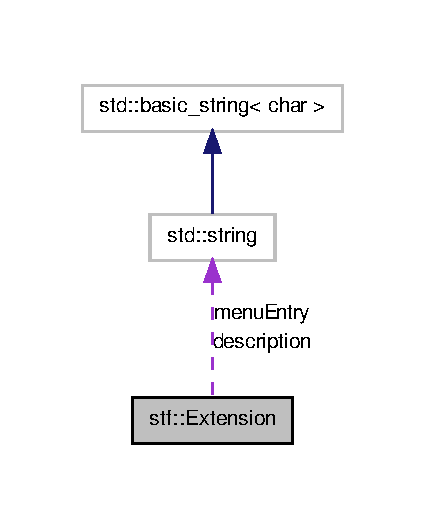
\includegraphics[width=204pt]{structstf_1_1Extension__coll__graph}
\end{center}
\end{figure}
\subsection*{Public Member Functions}
\begin{DoxyCompactItemize}
\item 
\hyperlink{structstf_1_1Extension_a279ba4a2a78e265c034450806715f789}{Extension} (const std::string \&menuEntry\_\-, void $\ast$pyFunc\_\-, const std::string \&description\_\-, bool requiresFile\_\-)
\begin{DoxyCompactList}\small\item\em Constructor. \item\end{DoxyCompactList}\item 
\hypertarget{structstf_1_1Extension_aa0e893a92ad0eca35620645ccadf12c1}{
\hyperlink{structstf_1_1Extension_aa0e893a92ad0eca35620645ccadf12c1}{$\sim$Extension} ()}
\label{structstf_1_1Extension_aa0e893a92ad0eca35620645ccadf12c1}

\begin{DoxyCompactList}\small\item\em Destructor. \item\end{DoxyCompactList}\end{DoxyCompactItemize}
\subsection*{Public Attributes}
\begin{DoxyCompactItemize}
\item 
int \hyperlink{structstf_1_1Extension_a069888104cfb479873e3da55e7c049d2}{id}
\item 
std::string \hyperlink{structstf_1_1Extension_a6e83222a3ed4de95ed36b143a6ee1913}{menuEntry}
\item 
void $\ast$ \hyperlink{structstf_1_1Extension_a2c2aeac701f3925233924aff9d1466b8}{pyFunc}
\item 
std::string \hyperlink{structstf_1_1Extension_a432e0a68c4052944bc5e9b679f688ad7}{description}
\item 
bool \hyperlink{structstf_1_1Extension_abaef4f6bdc9af533d706344c40ae4cf4}{requiresFile}
\end{DoxyCompactItemize}
\subsection*{Static Public Attributes}
\begin{DoxyCompactItemize}
\item 
static int \hyperlink{structstf_1_1Extension_a143b2d64266f86fe54937c98fdb59c32}{n\_\-extensions}
\end{DoxyCompactItemize}


\subsection{Detailed Description}
User-\/defined Python extension. Class used for extending Stimfit's functionality: The client supplies a new menu entry and a Python function that will be called upon selection of that entry. 

\subsection{Constructor \& Destructor Documentation}
\hypertarget{structstf_1_1Extension_a279ba4a2a78e265c034450806715f789}{
\index{stf::Extension@{stf::Extension}!Extension@{Extension}}
\index{Extension@{Extension}!stf::Extension@{stf::Extension}}
\subsubsection[{Extension}]{\setlength{\rightskip}{0pt plus 5cm}stf::Extension::Extension (
\begin{DoxyParamCaption}
\item[{const std::string \&}]{menuEntry\_\-, }
\item[{void $\ast$}]{pyFunc\_\-, }
\item[{const std::string \&}]{description\_\-, }
\item[{bool}]{requiresFile\_\-}
\end{DoxyParamCaption}
)\hspace{0.3cm}{\ttfamily  \mbox{[}inline\mbox{]}}}}
\label{structstf_1_1Extension_a279ba4a2a78e265c034450806715f789}


Constructor. 


\begin{DoxyParams}{Parameters}
{\em menuEntry\_\-} & Menu entry string for this extension. \\
\hline
{\em pyFunc\_\-} & Python function to be called. \\
\hline
{\em description\_\-} & Description for this function. \\
\hline
{\em requiresFile\_\-} & Whether a file needs to be open for this function to work \\
\hline
\end{DoxyParams}


References n\_\-extensions.



\subsection{Member Data Documentation}
\hypertarget{structstf_1_1Extension_a432e0a68c4052944bc5e9b679f688ad7}{
\index{stf::Extension@{stf::Extension}!description@{description}}
\index{description@{description}!stf::Extension@{stf::Extension}}
\subsubsection[{description}]{\setlength{\rightskip}{0pt plus 5cm}std::string {\bf stf::Extension::description}}}
\label{structstf_1_1Extension_a432e0a68c4052944bc5e9b679f688ad7}
Description for this function. \hypertarget{structstf_1_1Extension_a069888104cfb479873e3da55e7c049d2}{
\index{stf::Extension@{stf::Extension}!id@{id}}
\index{id@{id}!stf::Extension@{stf::Extension}}
\subsubsection[{id}]{\setlength{\rightskip}{0pt plus 5cm}int {\bf stf::Extension::id}}}
\label{structstf_1_1Extension_a069888104cfb479873e3da55e7c049d2}
The extension id; set automatically upon construction, so don't touch. \hypertarget{structstf_1_1Extension_a6e83222a3ed4de95ed36b143a6ee1913}{
\index{stf::Extension@{stf::Extension}!menuEntry@{menuEntry}}
\index{menuEntry@{menuEntry}!stf::Extension@{stf::Extension}}
\subsubsection[{menuEntry}]{\setlength{\rightskip}{0pt plus 5cm}std::string {\bf stf::Extension::menuEntry}}}
\label{structstf_1_1Extension_a6e83222a3ed4de95ed36b143a6ee1913}
Menu entry string for this extension. \hypertarget{structstf_1_1Extension_a143b2d64266f86fe54937c98fdb59c32}{
\index{stf::Extension@{stf::Extension}!n\_\-extensions@{n\_\-extensions}}
\index{n\_\-extensions@{n\_\-extensions}!stf::Extension@{stf::Extension}}
\subsubsection[{n\_\-extensions}]{\setlength{\rightskip}{0pt plus 5cm}int {\bf stf::Extension::n\_\-extensions}\hspace{0.3cm}{\ttfamily  \mbox{[}static\mbox{]}}}}
\label{structstf_1_1Extension_a143b2d64266f86fe54937c98fdb59c32}
Static extension counter. Initialised in extensions/extensions.cpp. 

Referenced by Extension().

\hypertarget{structstf_1_1Extension_a2c2aeac701f3925233924aff9d1466b8}{
\index{stf::Extension@{stf::Extension}!pyFunc@{pyFunc}}
\index{pyFunc@{pyFunc}!stf::Extension@{stf::Extension}}
\subsubsection[{pyFunc}]{\setlength{\rightskip}{0pt plus 5cm}void$\ast$ {\bf stf::Extension::pyFunc}}}
\label{structstf_1_1Extension_a2c2aeac701f3925233924aff9d1466b8}
Python function to be called. \hypertarget{structstf_1_1Extension_abaef4f6bdc9af533d706344c40ae4cf4}{
\index{stf::Extension@{stf::Extension}!requiresFile@{requiresFile}}
\index{requiresFile@{requiresFile}!stf::Extension@{stf::Extension}}
\subsubsection[{requiresFile}]{\setlength{\rightskip}{0pt plus 5cm}bool {\bf stf::Extension::requiresFile}}}
\label{structstf_1_1Extension_abaef4f6bdc9af533d706344c40ae4cf4}
Whether a file needs to be open for this function to work 

The documentation for this struct was generated from the following file:\begin{DoxyCompactItemize}
\item 
src/core/\hyperlink{stimdefs_8h}{stimdefs.h}\end{DoxyCompactItemize}

\hypertarget{structstf_1_1ifstreamMan}{
\section{stf::ifstreamMan Struct Reference}
\label{structstf_1_1ifstreamMan}\index{stf::ifstreamMan@{stf::ifstreamMan}}
}


Resource manager for ifstream objects.  




{\ttfamily \#include $<$stimdefs.h$>$}

\subsection*{Public Member Functions}
\begin{DoxyCompactItemize}
\item 
\hyperlink{structstf_1_1ifstreamMan_a263e597e796869b2ba33d8c1c1710eda}{ifstreamMan} (const \hyperlink{classwxString}{wxString} \&filename)
\begin{DoxyCompactList}\small\item\em Constructor. \item\end{DoxyCompactList}\item 
\hypertarget{structstf_1_1ifstreamMan_a8dfe92a7e07d7002c112e2fd1108ac4a}{
\hyperlink{structstf_1_1ifstreamMan_a8dfe92a7e07d7002c112e2fd1108ac4a}{$\sim$ifstreamMan} ()}
\label{structstf_1_1ifstreamMan_a8dfe92a7e07d7002c112e2fd1108ac4a}

\begin{DoxyCompactList}\small\item\em Destructor. \item\end{DoxyCompactList}\end{DoxyCompactItemize}
\subsection*{Public Attributes}
\begin{DoxyCompactItemize}
\item 
\hypertarget{structstf_1_1ifstreamMan_a383b301d80c1582e2a41f41b2cdf132b}{
wxFFile \hyperlink{structstf_1_1ifstreamMan_a383b301d80c1582e2a41f41b2cdf132b}{myStream}}
\label{structstf_1_1ifstreamMan_a383b301d80c1582e2a41f41b2cdf132b}

\begin{DoxyCompactList}\small\item\em The managed stream. \item\end{DoxyCompactList}\end{DoxyCompactItemize}


\subsection{Detailed Description}
Resource manager for ifstream objects. 

\subsection{Constructor \& Destructor Documentation}
\hypertarget{structstf_1_1ifstreamMan_a263e597e796869b2ba33d8c1c1710eda}{
\index{stf::ifstreamMan@{stf::ifstreamMan}!ifstreamMan@{ifstreamMan}}
\index{ifstreamMan@{ifstreamMan}!stf::ifstreamMan@{stf::ifstreamMan}}
\subsubsection[{ifstreamMan}]{\setlength{\rightskip}{0pt plus 5cm}stf::ifstreamMan::ifstreamMan (
\begin{DoxyParamCaption}
\item[{const {\bf wxString} \&}]{filename}
\end{DoxyParamCaption}
)\hspace{0.3cm}{\ttfamily  \mbox{[}inline\mbox{]}}}}
\label{structstf_1_1ifstreamMan_a263e597e796869b2ba33d8c1c1710eda}


Constructor. 

See fstream documentation for details 

The documentation for this struct was generated from the following file:\begin{DoxyCompactItemize}
\item 
src/core/\hyperlink{stimdefs_8h}{stimdefs.h}\end{DoxyCompactItemize}

\hypertarget{structstf_1_1ofstreamMan}{
\section{stf::ofstreamMan Struct Reference}
\label{structstf_1_1ofstreamMan}\index{stf::ofstreamMan@{stf::ofstreamMan}}
}


Resource manager for ofstream objects.  




{\ttfamily \#include $<$stimdefs.h$>$}

\subsection*{Public Member Functions}
\begin{DoxyCompactItemize}
\item 
\hyperlink{structstf_1_1ofstreamMan_af35f6aa35d2d5fa6c26b70240201e271}{ofstreamMan} (const \hyperlink{classwxString}{wxString} \&filename)
\begin{DoxyCompactList}\small\item\em Constructor. \item\end{DoxyCompactList}\item 
\hypertarget{structstf_1_1ofstreamMan_a97a2b8af26519413012685fb6596b1ec}{
\hyperlink{structstf_1_1ofstreamMan_a97a2b8af26519413012685fb6596b1ec}{$\sim$ofstreamMan} ()}
\label{structstf_1_1ofstreamMan_a97a2b8af26519413012685fb6596b1ec}

\begin{DoxyCompactList}\small\item\em Destructor. \item\end{DoxyCompactList}\end{DoxyCompactItemize}
\subsection*{Public Attributes}
\begin{DoxyCompactItemize}
\item 
\hypertarget{structstf_1_1ofstreamMan_a9dd17bbd6aadc32a2d70a05bafd5c75e}{
wxFFile \hyperlink{structstf_1_1ofstreamMan_a9dd17bbd6aadc32a2d70a05bafd5c75e}{myStream}}
\label{structstf_1_1ofstreamMan_a9dd17bbd6aadc32a2d70a05bafd5c75e}

\begin{DoxyCompactList}\small\item\em The managed stream. \item\end{DoxyCompactList}\end{DoxyCompactItemize}


\subsection{Detailed Description}
Resource manager for ofstream objects. 

\subsection{Constructor \& Destructor Documentation}
\hypertarget{structstf_1_1ofstreamMan_af35f6aa35d2d5fa6c26b70240201e271}{
\index{stf::ofstreamMan@{stf::ofstreamMan}!ofstreamMan@{ofstreamMan}}
\index{ofstreamMan@{ofstreamMan}!stf::ofstreamMan@{stf::ofstreamMan}}
\subsubsection[{ofstreamMan}]{\setlength{\rightskip}{0pt plus 5cm}stf::ofstreamMan::ofstreamMan (
\begin{DoxyParamCaption}
\item[{const {\bf wxString} \&}]{filename}
\end{DoxyParamCaption}
)\hspace{0.3cm}{\ttfamily  \mbox{[}inline\mbox{]}}}}
\label{structstf_1_1ofstreamMan_af35f6aa35d2d5fa6c26b70240201e271}


Constructor. 

See fstream documentation for details 

The documentation for this struct was generated from the following file:\begin{DoxyCompactItemize}
\item 
src/core/\hyperlink{stimdefs_8h}{stimdefs.h}\end{DoxyCompactItemize}

\hypertarget{structstf_1_1parInfo}{
\section{stf::parInfo Struct Reference}
\label{structstf_1_1parInfo}\index{stf::parInfo@{stf::parInfo}}
}


Information about parameters used in \hyperlink{structstf_1_1storedFunc}{storedFunc}.  




{\ttfamily \#include $<$stimdefs.h$>$}



Collaboration diagram for stf::parInfo:
\nopagebreak
\begin{figure}[H]
\begin{center}
\leavevmode
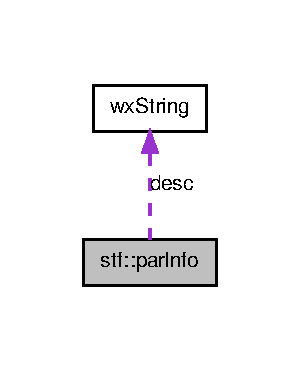
\includegraphics[width=144pt]{structstf_1_1parInfo__coll__graph}
\end{center}
\end{figure}
\subsection*{Public Member Functions}
\begin{DoxyCompactItemize}
\item 
\hypertarget{structstf_1_1parInfo_a785b7e816901e1a9d9a1d1081028e74d}{
\hyperlink{structstf_1_1parInfo_a785b7e816901e1a9d9a1d1081028e74d}{parInfo} ()}
\label{structstf_1_1parInfo_a785b7e816901e1a9d9a1d1081028e74d}

\begin{DoxyCompactList}\small\item\em Default constructor. \item\end{DoxyCompactList}\item 
\hyperlink{structstf_1_1parInfo_ac5abdf716cbc842663539219eafb2ca4}{parInfo} (const \hyperlink{classwxString}{wxString} \&desc\_\-, bool toFit\_\-, bool constrained\_\-=false, double constr\_\-lb\_\-=0, double constr\_\-ub\_\-=0, \hyperlink{group__stfgen_ga775530afebda38e8138e8eb1401a0e01}{Scale} scale\_\-=noscale, \hyperlink{group__stfgen_ga775530afebda38e8138e8eb1401a0e01}{Scale} unscale\_\-=noscale)
\begin{DoxyCompactList}\small\item\em Constructor. \item\end{DoxyCompactList}\end{DoxyCompactItemize}
\subsection*{Public Attributes}
\begin{DoxyCompactItemize}
\item 
\hyperlink{classwxString}{wxString} \hyperlink{structstf_1_1parInfo_a9fd83d6be04108ad0947ff0e336bb4c4}{desc}
\item 
bool \hyperlink{structstf_1_1parInfo_a204d67206f39c8e7a2efcfbd757f447b}{toFit}
\item 
bool \hyperlink{structstf_1_1parInfo_acd5ad5c8721d2d0275932671c81bac1a}{constrained}
\item 
double \hyperlink{structstf_1_1parInfo_a78f17a10d539858d71539135ee4e46ce}{constr\_\-lb}
\item 
double \hyperlink{structstf_1_1parInfo_a0cd313970fe68a4dc1ede892029f545a}{constr\_\-ub}
\item 
\hyperlink{group__stfgen_ga775530afebda38e8138e8eb1401a0e01}{Scale} \hyperlink{structstf_1_1parInfo_abfcd4e222d78f17e915b587457c98a37}{scale}
\item 
\hyperlink{group__stfgen_ga775530afebda38e8138e8eb1401a0e01}{Scale} \hyperlink{structstf_1_1parInfo_a5c3e4eecc13bbd9351ee862c1ddc9829}{unscale}
\end{DoxyCompactItemize}


\subsection{Detailed Description}
Information about parameters used in \hyperlink{structstf_1_1storedFunc}{storedFunc}. Contains information about a function's parameters used in \hyperlink{structstf_1_1storedFunc}{storedFunc} (see below). The client supplies a description (desc) and determines whether the parameter is to be fitted (toFit==true) or to be kept constant (toFit==false). 

\subsection{Constructor \& Destructor Documentation}
\hypertarget{structstf_1_1parInfo_ac5abdf716cbc842663539219eafb2ca4}{
\index{stf::parInfo@{stf::parInfo}!parInfo@{parInfo}}
\index{parInfo@{parInfo}!stf::parInfo@{stf::parInfo}}
\subsubsection[{parInfo}]{\setlength{\rightskip}{0pt plus 5cm}stf::parInfo::parInfo (
\begin{DoxyParamCaption}
\item[{const {\bf wxString} \&}]{desc\_\-, }
\item[{bool}]{toFit\_\-, }
\item[{bool}]{constrained\_\- = {\ttfamily false}, }
\item[{double}]{constr\_\-lb\_\- = {\ttfamily 0}, }
\item[{double}]{constr\_\-ub\_\- = {\ttfamily 0}, }
\item[{{\bf Scale}}]{scale\_\- = {\ttfamily noscale}, }
\item[{{\bf Scale}}]{unscale\_\- = {\ttfamily noscale}}
\end{DoxyParamCaption}
)\hspace{0.3cm}{\ttfamily  \mbox{[}inline\mbox{]}}}}
\label{structstf_1_1parInfo_ac5abdf716cbc842663539219eafb2ca4}


Constructor. 


\begin{DoxyParams}{Parameters}
{\em desc\_\-} & Parameter description string \\
\hline
{\em toFit\_\-} & true if this parameter should be fitted, false if it should be kept fixed. \\
\hline
{\em constrained\_\-} & true if this is a constrained fit \\
\hline
{\em constr\_\-lb\_\-} & lower bound for constrained fit \\
\hline
{\em constr\_\-ub\_\-} & upper bound for constrained fit \\
\hline
{\em scale\_\-} & scaling function \\
\hline
{\em unscale\_\-} & unscaling function \\
\hline
\end{DoxyParams}


\subsection{Member Data Documentation}
\hypertarget{structstf_1_1parInfo_a78f17a10d539858d71539135ee4e46ce}{
\index{stf::parInfo@{stf::parInfo}!constr\_\-lb@{constr\_\-lb}}
\index{constr\_\-lb@{constr\_\-lb}!stf::parInfo@{stf::parInfo}}
\subsubsection[{constr\_\-lb}]{\setlength{\rightskip}{0pt plus 5cm}double {\bf stf::parInfo::constr\_\-lb}}}
\label{structstf_1_1parInfo_a78f17a10d539858d71539135ee4e46ce}
Lower boundary for box-\/constrained fits \hypertarget{structstf_1_1parInfo_a0cd313970fe68a4dc1ede892029f545a}{
\index{stf::parInfo@{stf::parInfo}!constr\_\-ub@{constr\_\-ub}}
\index{constr\_\-ub@{constr\_\-ub}!stf::parInfo@{stf::parInfo}}
\subsubsection[{constr\_\-ub}]{\setlength{\rightskip}{0pt plus 5cm}double {\bf stf::parInfo::constr\_\-ub}}}
\label{structstf_1_1parInfo_a0cd313970fe68a4dc1ede892029f545a}
Upper boundary for box-\/constrained fits \hypertarget{structstf_1_1parInfo_acd5ad5c8721d2d0275932671c81bac1a}{
\index{stf::parInfo@{stf::parInfo}!constrained@{constrained}}
\index{constrained@{constrained}!stf::parInfo@{stf::parInfo}}
\subsubsection[{constrained}]{\setlength{\rightskip}{0pt plus 5cm}bool {\bf stf::parInfo::constrained}}}
\label{structstf_1_1parInfo_acd5ad5c8721d2d0275932671c81bac1a}
true if this parameter should be constrained \hypertarget{structstf_1_1parInfo_a9fd83d6be04108ad0947ff0e336bb4c4}{
\index{stf::parInfo@{stf::parInfo}!desc@{desc}}
\index{desc@{desc}!stf::parInfo@{stf::parInfo}}
\subsubsection[{desc}]{\setlength{\rightskip}{0pt plus 5cm}{\bf wxString} {\bf stf::parInfo::desc}}}
\label{structstf_1_1parInfo_a9fd83d6be04108ad0947ff0e336bb4c4}
Parameter description string \hypertarget{structstf_1_1parInfo_abfcd4e222d78f17e915b587457c98a37}{
\index{stf::parInfo@{stf::parInfo}!scale@{scale}}
\index{scale@{scale}!stf::parInfo@{stf::parInfo}}
\subsubsection[{scale}]{\setlength{\rightskip}{0pt plus 5cm}{\bf Scale} {\bf stf::parInfo::scale}}}
\label{structstf_1_1parInfo_abfcd4e222d78f17e915b587457c98a37}
Scaling function for this parameter \hypertarget{structstf_1_1parInfo_a204d67206f39c8e7a2efcfbd757f447b}{
\index{stf::parInfo@{stf::parInfo}!toFit@{toFit}}
\index{toFit@{toFit}!stf::parInfo@{stf::parInfo}}
\subsubsection[{toFit}]{\setlength{\rightskip}{0pt plus 5cm}bool {\bf stf::parInfo::toFit}}}
\label{structstf_1_1parInfo_a204d67206f39c8e7a2efcfbd757f447b}
true if this parameter should be fitted, false if it should be kept fixed. \hypertarget{structstf_1_1parInfo_a5c3e4eecc13bbd9351ee862c1ddc9829}{
\index{stf::parInfo@{stf::parInfo}!unscale@{unscale}}
\index{unscale@{unscale}!stf::parInfo@{stf::parInfo}}
\subsubsection[{unscale}]{\setlength{\rightskip}{0pt plus 5cm}{\bf Scale} {\bf stf::parInfo::unscale}}}
\label{structstf_1_1parInfo_a5c3e4eecc13bbd9351ee862c1ddc9829}
Unscaling function for this parameter 

The documentation for this struct was generated from the following file:\begin{DoxyCompactItemize}
\item 
src/core/\hyperlink{stimdefs_8h}{stimdefs.h}\end{DoxyCompactItemize}

\hypertarget{structstf_1_1Plugin}{
\section{stf::Plugin Struct Reference}
\label{structstf_1_1Plugin}\index{stf::Plugin@{stf::Plugin}}
}


User-\/defined plugin.  




{\ttfamily \#include $<$stimdefs.h$>$}



Collaboration diagram for stf::Plugin:
\nopagebreak
\begin{figure}[H]
\begin{center}
\leavevmode
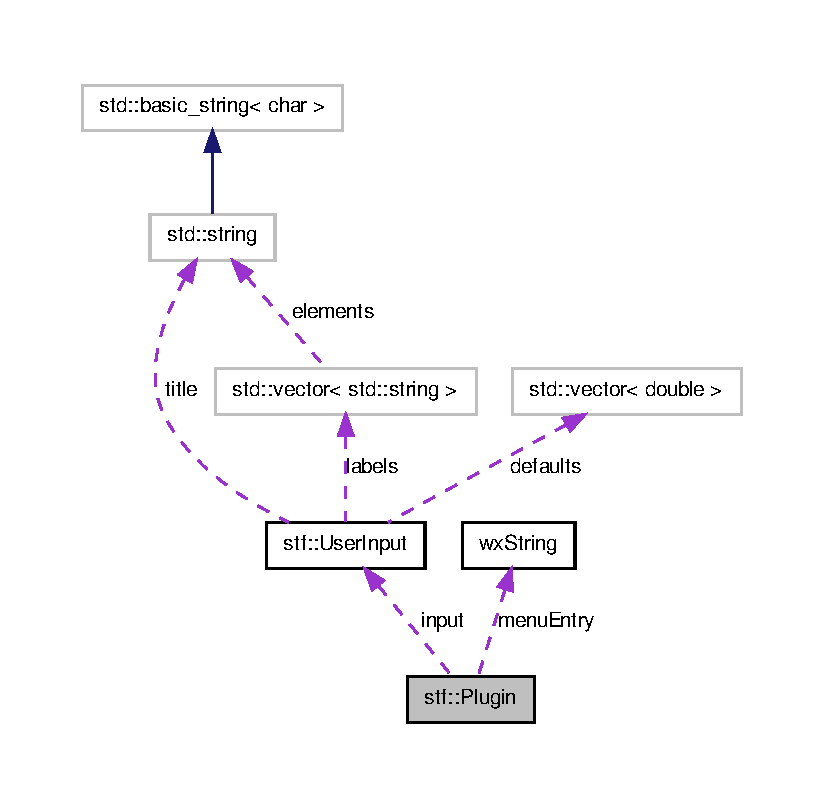
\includegraphics[width=396pt]{structstf_1_1Plugin__coll__graph}
\end{center}
\end{figure}
\subsection*{Public Member Functions}
\begin{DoxyCompactItemize}
\item 
\hyperlink{structstf_1_1Plugin_a0609473477d0237371571bfe143536bf}{Plugin} (const \hyperlink{classwxString}{wxString} \&menuEntry\_\-, const \hyperlink{group__stfgen_gaa37601710b061d50b53ceeab1e7a9dd2}{PluginFunc} \&pluginFunc\_\-, const \hyperlink{structstf_1_1UserInput}{UserInput} \&input\_\-=\hyperlink{structstf_1_1UserInput}{UserInput}())
\begin{DoxyCompactList}\small\item\em Constructor. \item\end{DoxyCompactList}\item 
\hypertarget{structstf_1_1Plugin_a2347a780c8b165fd604f8bd5656630a5}{
\hyperlink{structstf_1_1Plugin_a2347a780c8b165fd604f8bd5656630a5}{$\sim$Plugin} ()}
\label{structstf_1_1Plugin_a2347a780c8b165fd604f8bd5656630a5}

\begin{DoxyCompactList}\small\item\em Destructor. \item\end{DoxyCompactList}\end{DoxyCompactItemize}
\subsection*{Public Attributes}
\begin{DoxyCompactItemize}
\item 
int \hyperlink{structstf_1_1Plugin_a417ea89eae1a8fbd21e7c7488d14fd7d}{id}
\item 
\hyperlink{classwxString}{wxString} \hyperlink{structstf_1_1Plugin_a9e7060c1a895ba6ea04250c2c1313272}{menuEntry}
\item 
\hyperlink{group__stfgen_gaa37601710b061d50b53ceeab1e7a9dd2}{PluginFunc} \hyperlink{structstf_1_1Plugin_aebef99c1f1bd1d6c69ff8fb31988d22d}{pluginFunc}
\item 
\hyperlink{structstf_1_1UserInput}{UserInput} \hyperlink{structstf_1_1Plugin_a53713a074aabf4d0e873d9d13b1e60f3}{input}
\end{DoxyCompactItemize}
\subsection*{Static Public Attributes}
\begin{DoxyCompactItemize}
\item 
static int \hyperlink{structstf_1_1Plugin_a41eba3414a715e63c4dfff9fc2d53851}{n\_\-plugins}
\end{DoxyCompactItemize}


\subsection{Detailed Description}
User-\/defined plugin. Class used for extending Stimfit's functionality: The client supplies a new menu entry and an ExtFunc that will be called upon selection of that entry. 

\subsection{Constructor \& Destructor Documentation}
\hypertarget{structstf_1_1Plugin_a0609473477d0237371571bfe143536bf}{
\index{stf::Plugin@{stf::Plugin}!Plugin@{Plugin}}
\index{Plugin@{Plugin}!stf::Plugin@{stf::Plugin}}
\subsubsection[{Plugin}]{\setlength{\rightskip}{0pt plus 5cm}stf::Plugin::Plugin (
\begin{DoxyParamCaption}
\item[{const {\bf wxString} \&}]{menuEntry\_\-, }
\item[{const {\bf PluginFunc} \&}]{pluginFunc\_\-, }
\item[{const {\bf UserInput} \&}]{input\_\- = {\ttfamily {\bf UserInput}()}}
\end{DoxyParamCaption}
)\hspace{0.3cm}{\ttfamily  \mbox{[}inline\mbox{]}}}}
\label{structstf_1_1Plugin_a0609473477d0237371571bfe143536bf}


Constructor. 


\begin{DoxyParams}{Parameters}
{\em menuEntry\_\-} & Menu entry string for this plugin. \\
\hline
{\em pluginFunc\_\-} & Function to be executed by this plugin. \\
\hline
{\em input\_\-} & Dialog entries required by this plugin. \\
\hline
\end{DoxyParams}


References n\_\-plugins.



\subsection{Member Data Documentation}
\hypertarget{structstf_1_1Plugin_a417ea89eae1a8fbd21e7c7488d14fd7d}{
\index{stf::Plugin@{stf::Plugin}!id@{id}}
\index{id@{id}!stf::Plugin@{stf::Plugin}}
\subsubsection[{id}]{\setlength{\rightskip}{0pt plus 5cm}int {\bf stf::Plugin::id}}}
\label{structstf_1_1Plugin_a417ea89eae1a8fbd21e7c7488d14fd7d}
The plugin id; set automatically upon construction, so don't touch. \hypertarget{structstf_1_1Plugin_a53713a074aabf4d0e873d9d13b1e60f3}{
\index{stf::Plugin@{stf::Plugin}!input@{input}}
\index{input@{input}!stf::Plugin@{stf::Plugin}}
\subsubsection[{input}]{\setlength{\rightskip}{0pt plus 5cm}{\bf UserInput} {\bf stf::Plugin::input}}}
\label{structstf_1_1Plugin_a53713a074aabf4d0e873d9d13b1e60f3}
Dialog entries \hypertarget{structstf_1_1Plugin_a9e7060c1a895ba6ea04250c2c1313272}{
\index{stf::Plugin@{stf::Plugin}!menuEntry@{menuEntry}}
\index{menuEntry@{menuEntry}!stf::Plugin@{stf::Plugin}}
\subsubsection[{menuEntry}]{\setlength{\rightskip}{0pt plus 5cm}{\bf wxString} {\bf stf::Plugin::menuEntry}}}
\label{structstf_1_1Plugin_a9e7060c1a895ba6ea04250c2c1313272}
Menu entry string for this plugin. \hypertarget{structstf_1_1Plugin_a41eba3414a715e63c4dfff9fc2d53851}{
\index{stf::Plugin@{stf::Plugin}!n\_\-plugins@{n\_\-plugins}}
\index{n\_\-plugins@{n\_\-plugins}!stf::Plugin@{stf::Plugin}}
\subsubsection[{n\_\-plugins}]{\setlength{\rightskip}{0pt plus 5cm}int {\bf stf::Plugin::n\_\-plugins}\hspace{0.3cm}{\ttfamily  \mbox{[}static\mbox{]}}}}
\label{structstf_1_1Plugin_a41eba3414a715e63c4dfff9fc2d53851}
Static plugin counter. Initialised in plugins/plugins.cpp. 

Referenced by Plugin().

\hypertarget{structstf_1_1Plugin_aebef99c1f1bd1d6c69ff8fb31988d22d}{
\index{stf::Plugin@{stf::Plugin}!pluginFunc@{pluginFunc}}
\index{pluginFunc@{pluginFunc}!stf::Plugin@{stf::Plugin}}
\subsubsection[{pluginFunc}]{\setlength{\rightskip}{0pt plus 5cm}{\bf PluginFunc} {\bf stf::Plugin::pluginFunc}}}
\label{structstf_1_1Plugin_aebef99c1f1bd1d6c69ff8fb31988d22d}
The function to be executed by this plugin. 

The documentation for this struct was generated from the following file:\begin{DoxyCompactItemize}
\item 
src/core/\hyperlink{stimdefs_8h}{stimdefs.h}\end{DoxyCompactItemize}

\hypertarget{structstf_1_1PyMarker}{
\section{stf::PyMarker Struct Reference}
\label{structstf_1_1PyMarker}\index{stf::PyMarker@{stf::PyMarker}}
}


A marker that can be set from Python.  




{\ttfamily \#include $<$stimdefs.h$>$}

\subsection*{Public Member Functions}
\begin{DoxyCompactItemize}
\item 
\hyperlink{structstf_1_1PyMarker_aa95183fe49a03c885576ea21e5f5778c}{PyMarker} (double xv, double yv)
\begin{DoxyCompactList}\small\item\em Constructor. \item\end{DoxyCompactList}\end{DoxyCompactItemize}
\subsection*{Public Attributes}
\begin{DoxyCompactItemize}
\item 
double \hyperlink{structstf_1_1PyMarker_a6ae48b5897b21ccea4511db938dd46ce}{x}
\item 
double \hyperlink{structstf_1_1PyMarker_a0d54ef4d998f32b1e5745c2fa7911fcd}{y}
\end{DoxyCompactItemize}


\subsection{Detailed Description}
A marker that can be set from Python. A pair of x,y coordinates 

\subsection{Constructor \& Destructor Documentation}
\hypertarget{structstf_1_1PyMarker_aa95183fe49a03c885576ea21e5f5778c}{
\index{stf::PyMarker@{stf::PyMarker}!PyMarker@{PyMarker}}
\index{PyMarker@{PyMarker}!stf::PyMarker@{stf::PyMarker}}
\subsubsection[{PyMarker}]{\setlength{\rightskip}{0pt plus 5cm}stf::PyMarker::PyMarker (
\begin{DoxyParamCaption}
\item[{double}]{xv, }
\item[{double}]{yv}
\end{DoxyParamCaption}
)\hspace{0.3cm}{\ttfamily  \mbox{[}inline\mbox{]}}}}
\label{structstf_1_1PyMarker_aa95183fe49a03c885576ea21e5f5778c}


Constructor. 


\begin{DoxyParams}{Parameters}
{\em xv} & x-\/coordinate. \\
\hline
{\em yv} & y-\/coordinate. \\
\hline
\end{DoxyParams}


\subsection{Member Data Documentation}
\hypertarget{structstf_1_1PyMarker_a6ae48b5897b21ccea4511db938dd46ce}{
\index{stf::PyMarker@{stf::PyMarker}!x@{x}}
\index{x@{x}!stf::PyMarker@{stf::PyMarker}}
\subsubsection[{x}]{\setlength{\rightskip}{0pt plus 5cm}double {\bf stf::PyMarker::x}}}
\label{structstf_1_1PyMarker_a6ae48b5897b21ccea4511db938dd46ce}
x-\/coordinate in units of sampling points \hypertarget{structstf_1_1PyMarker_a0d54ef4d998f32b1e5745c2fa7911fcd}{
\index{stf::PyMarker@{stf::PyMarker}!y@{y}}
\index{y@{y}!stf::PyMarker@{stf::PyMarker}}
\subsubsection[{y}]{\setlength{\rightskip}{0pt plus 5cm}double {\bf stf::PyMarker::y}}}
\label{structstf_1_1PyMarker_a0d54ef4d998f32b1e5745c2fa7911fcd}
y-\/coordinate in trace units (e.g. mV) 

The documentation for this struct was generated from the following file:\begin{DoxyCompactItemize}
\item 
src/core/\hyperlink{stimdefs_8h}{stimdefs.h}\end{DoxyCompactItemize}

\hypertarget{structstf_1_1storedFunc}{
\section{stf::storedFunc Struct Reference}
\label{structstf_1_1storedFunc}\index{stf::storedFunc@{stf::storedFunc}}
}


Function used for least-\/squares fitting.  




{\ttfamily \#include $<$stimdefs.h$>$}



Collaboration diagram for stf::storedFunc:
\nopagebreak
\begin{figure}[H]
\begin{center}
\leavevmode
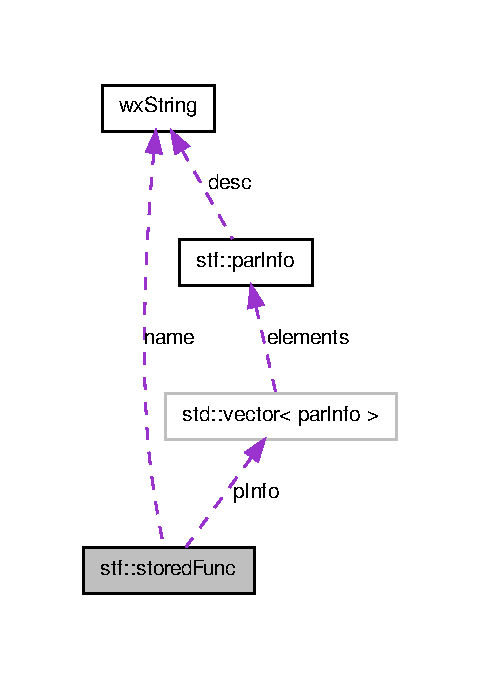
\includegraphics[width=230pt]{structstf_1_1storedFunc__coll__graph}
\end{center}
\end{figure}
\subsection*{Public Member Functions}
\begin{DoxyCompactItemize}
\item 
\hyperlink{structstf_1_1storedFunc_a6cfde3ff81a2297aaf4b33ee46a9a7e9}{storedFunc} (const \hyperlink{classwxString}{wxString} \&name\_\-, const std::vector$<$ \hyperlink{structstf_1_1parInfo}{parInfo} $>$ \&pInfo\_\-, const \hyperlink{group__stfgen_ga11d6ec55abceacf5fdd47f9fc889d9a3}{Func} \&func\_\-, const \hyperlink{group__stfgen_ga15ccefdb3c4b758564e73f080639ff98}{Init} \&init\_\-, const \hyperlink{group__stfgen_ga77f3e621f1771784f2befaeb3d1ac4fb}{Jac} \&jac\_\-, bool hasJac\_\-=true, const \hyperlink{group__stfgen_ga66542f63882a99158a17cdc977eac5e8}{Output} \&output\_\-=defaultOutput)
\begin{DoxyCompactList}\small\item\em Constructor. \item\end{DoxyCompactList}\item 
\hypertarget{structstf_1_1storedFunc_a058a7ae12ebbaf5dd5f42eb69052b6e8}{
\hyperlink{structstf_1_1storedFunc_a058a7ae12ebbaf5dd5f42eb69052b6e8}{$\sim$storedFunc} ()}
\label{structstf_1_1storedFunc_a058a7ae12ebbaf5dd5f42eb69052b6e8}

\begin{DoxyCompactList}\small\item\em Destructor. \item\end{DoxyCompactList}\end{DoxyCompactItemize}
\subsection*{Public Attributes}
\begin{DoxyCompactItemize}
\item 
\hyperlink{classwxString}{wxString} \hyperlink{structstf_1_1storedFunc_ac1fe235432b5de9f93817a573b6d9946}{name}
\item 
std::vector$<$ \hyperlink{structstf_1_1parInfo}{parInfo} $>$ \hyperlink{structstf_1_1storedFunc_a2f09fc5276140a85ad4fa61bccc3fd61}{pInfo}
\item 
\hyperlink{group__stfgen_ga11d6ec55abceacf5fdd47f9fc889d9a3}{Func} \hyperlink{structstf_1_1storedFunc_a3ec6459b20161c0331f69902d219e5f4}{func}
\item 
\hyperlink{group__stfgen_ga15ccefdb3c4b758564e73f080639ff98}{Init} \hyperlink{structstf_1_1storedFunc_a825fd7a72e67915cde6439afe8010840}{init}
\item 
\hyperlink{group__stfgen_ga77f3e621f1771784f2befaeb3d1ac4fb}{Jac} \hyperlink{structstf_1_1storedFunc_a5f97002993f83f9c162e2a9fde8125ea}{jac}
\item 
bool \hyperlink{structstf_1_1storedFunc_a26a0e3f68ef57d72e5fd8e967dc15911}{hasJac}
\item 
\hyperlink{group__stfgen_ga66542f63882a99158a17cdc977eac5e8}{Output} \hyperlink{structstf_1_1storedFunc_aad9e1ffc2999387f61578bf9f7461224}{output}
\end{DoxyCompactItemize}


\subsection{Detailed Description}
Function used for least-\/squares fitting. Objects of this class are used for fitting functions to data. The client supplies a function (func), its jacobian (jac), information about the function's parameters (pInfo) and a function to initialize the parameters (init). 

\subsection{Constructor \& Destructor Documentation}
\hypertarget{structstf_1_1storedFunc_a6cfde3ff81a2297aaf4b33ee46a9a7e9}{
\index{stf::storedFunc@{stf::storedFunc}!storedFunc@{storedFunc}}
\index{storedFunc@{storedFunc}!stf::storedFunc@{stf::storedFunc}}
\subsubsection[{storedFunc}]{\setlength{\rightskip}{0pt plus 5cm}stf::storedFunc::storedFunc (
\begin{DoxyParamCaption}
\item[{const {\bf wxString} \&}]{name\_\-, }
\item[{const std::vector$<$ {\bf parInfo} $>$ \&}]{pInfo\_\-, }
\item[{const {\bf Func} \&}]{func\_\-, }
\item[{const {\bf Init} \&}]{init\_\-, }
\item[{const {\bf Jac} \&}]{jac\_\-, }
\item[{bool}]{hasJac\_\- = {\ttfamily true}, }
\item[{const {\bf Output} \&}]{output\_\- = {\ttfamily defaultOutput}}
\end{DoxyParamCaption}
)\hspace{0.3cm}{\ttfamily  \mbox{[}inline\mbox{]}}}}
\label{structstf_1_1storedFunc_a6cfde3ff81a2297aaf4b33ee46a9a7e9}


Constructor. 


\begin{DoxyParams}{Parameters}
{\em name\_\-} & Plain function name. \\
\hline
{\em pInfo\_\-} & A vector containing information about the function parameters. \\
\hline
{\em func\_\-} & The function that will be fitted to the data. \\
\hline
{\em jac\_\-} & Jacobian of func\_\-. \\
\hline
{\em hasJac\_\-} & true if a Jacobian is available. \\
\hline
{\em init\_\-} & A function for initialising the parameters. \\
\hline
{\em output\_\-} & Output of the fit. \\
\hline
\end{DoxyParams}


\subsection{Member Data Documentation}
\hypertarget{structstf_1_1storedFunc_a3ec6459b20161c0331f69902d219e5f4}{
\index{stf::storedFunc@{stf::storedFunc}!func@{func}}
\index{func@{func}!stf::storedFunc@{stf::storedFunc}}
\subsubsection[{func}]{\setlength{\rightskip}{0pt plus 5cm}{\bf Func} {\bf stf::storedFunc::func}}}
\label{structstf_1_1storedFunc_a3ec6459b20161c0331f69902d219e5f4}
The function that will be fitted to the data. \hypertarget{structstf_1_1storedFunc_a26a0e3f68ef57d72e5fd8e967dc15911}{
\index{stf::storedFunc@{stf::storedFunc}!hasJac@{hasJac}}
\index{hasJac@{hasJac}!stf::storedFunc@{stf::storedFunc}}
\subsubsection[{hasJac}]{\setlength{\rightskip}{0pt plus 5cm}bool {\bf stf::storedFunc::hasJac}}}
\label{structstf_1_1storedFunc_a26a0e3f68ef57d72e5fd8e967dc15911}
True if the function has an analytic Jacobian. \hypertarget{structstf_1_1storedFunc_a825fd7a72e67915cde6439afe8010840}{
\index{stf::storedFunc@{stf::storedFunc}!init@{init}}
\index{init@{init}!stf::storedFunc@{stf::storedFunc}}
\subsubsection[{init}]{\setlength{\rightskip}{0pt plus 5cm}{\bf Init} {\bf stf::storedFunc::init}}}
\label{structstf_1_1storedFunc_a825fd7a72e67915cde6439afe8010840}
A function for initialising the parameters. \hypertarget{structstf_1_1storedFunc_a5f97002993f83f9c162e2a9fde8125ea}{
\index{stf::storedFunc@{stf::storedFunc}!jac@{jac}}
\index{jac@{jac}!stf::storedFunc@{stf::storedFunc}}
\subsubsection[{jac}]{\setlength{\rightskip}{0pt plus 5cm}{\bf Jac} {\bf stf::storedFunc::jac}}}
\label{structstf_1_1storedFunc_a5f97002993f83f9c162e2a9fde8125ea}
Jacobian of func. \hypertarget{structstf_1_1storedFunc_ac1fe235432b5de9f93817a573b6d9946}{
\index{stf::storedFunc@{stf::storedFunc}!name@{name}}
\index{name@{name}!stf::storedFunc@{stf::storedFunc}}
\subsubsection[{name}]{\setlength{\rightskip}{0pt plus 5cm}{\bf wxString} {\bf stf::storedFunc::name}}}
\label{structstf_1_1storedFunc_ac1fe235432b5de9f93817a573b6d9946}
Function name. \hypertarget{structstf_1_1storedFunc_aad9e1ffc2999387f61578bf9f7461224}{
\index{stf::storedFunc@{stf::storedFunc}!output@{output}}
\index{output@{output}!stf::storedFunc@{stf::storedFunc}}
\subsubsection[{output}]{\setlength{\rightskip}{0pt plus 5cm}{\bf Output} {\bf stf::storedFunc::output}}}
\label{structstf_1_1storedFunc_aad9e1ffc2999387f61578bf9f7461224}
Output of the fit. \hypertarget{structstf_1_1storedFunc_a2f09fc5276140a85ad4fa61bccc3fd61}{
\index{stf::storedFunc@{stf::storedFunc}!pInfo@{pInfo}}
\index{pInfo@{pInfo}!stf::storedFunc@{stf::storedFunc}}
\subsubsection[{pInfo}]{\setlength{\rightskip}{0pt plus 5cm}std::vector$<${\bf parInfo}$>$ {\bf stf::storedFunc::pInfo}}}
\label{structstf_1_1storedFunc_a2f09fc5276140a85ad4fa61bccc3fd61}
A vector containing information about the function parameters. 

The documentation for this struct was generated from the following file:\begin{DoxyCompactItemize}
\item 
src/core/\hyperlink{stimdefs_8h}{stimdefs.h}\end{DoxyCompactItemize}

\hypertarget{classstf_1_1Table}{
\section{stf::Table Class Reference}
\label{classstf_1_1Table}\index{stf::Table@{stf::Table}}
}


A table used for printing information.  




{\ttfamily \#include $<$stimdefs.h$>$}



Collaboration diagram for stf::Table:
\nopagebreak
\begin{figure}[H]
\begin{center}
\leavevmode
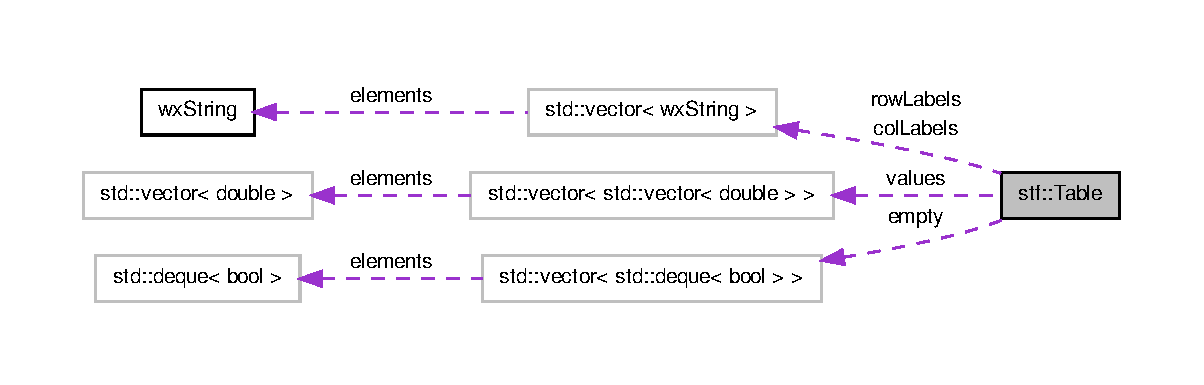
\includegraphics[width=400pt]{classstf_1_1Table__coll__graph}
\end{center}
\end{figure}
\subsection*{Public Member Functions}
\begin{DoxyCompactItemize}
\item 
\hyperlink{classstf_1_1Table_a1f1d6afbd987fe37bd82b1a48b81376c}{Table} (std::size\_\-t nRows, std::size\_\-t nCols)
\begin{DoxyCompactList}\small\item\em Constructor. \item\end{DoxyCompactList}\item 
\hyperlink{classstf_1_1Table_a305aa883ca1e57d53c4549e41ca0359c}{Table} (const std::map$<$ \hyperlink{classwxString}{wxString}, double $>$ \&map)
\begin{DoxyCompactList}\small\item\em Constructor. \item\end{DoxyCompactList}\item 
double \hyperlink{classstf_1_1Table_a04cc74be93cc5500bff4e3a14b64e138}{at} (std::size\_\-t row, std::size\_\-t col) const 
\begin{DoxyCompactList}\small\item\em Range-\/checked access. Returns a copy. Throws std::out\_\-of\_\-range if out of range. \item\end{DoxyCompactList}\item 
double \& \hyperlink{classstf_1_1Table_a1c2afdf17375d9597b48c7e6746ccf9f}{at} (std::size\_\-t row, std::size\_\-t col)
\begin{DoxyCompactList}\small\item\em Range-\/checked access. Returns a reference. Throws std::out\_\-of\_\-range if out of range. \item\end{DoxyCompactList}\item 
bool \hyperlink{classstf_1_1Table_a861ed4ad0902030911f7d397d9364e33}{IsEmpty} (std::size\_\-t row, std::size\_\-t col) const 
\begin{DoxyCompactList}\small\item\em Check whether a cell is empty. \item\end{DoxyCompactList}\item 
void \hyperlink{classstf_1_1Table_aafe151071912c07baee9ff503f914ae0}{SetEmpty} (std::size\_\-t row, std::size\_\-t col, bool value=true)
\begin{DoxyCompactList}\small\item\em Empties or un-\/empties a cell. \item\end{DoxyCompactList}\item 
void \hyperlink{classstf_1_1Table_ac690107b3da37447fcf81c8415a4bbf8}{SetRowLabel} (std::size\_\-t row, const \hyperlink{classwxString}{wxString} \&label)
\begin{DoxyCompactList}\small\item\em Sets the label of a row. \item\end{DoxyCompactList}\item 
void \hyperlink{classstf_1_1Table_acfb40b394d65fc6f3d6641b15516cfbe}{SetColLabel} (std::size\_\-t col, const \hyperlink{classwxString}{wxString} \&label)
\begin{DoxyCompactList}\small\item\em Sets the label of a column. \item\end{DoxyCompactList}\item 
const \hyperlink{classwxString}{wxString} \& \hyperlink{classstf_1_1Table_ad128a17e4345ef497f2f3cb3d24b73b4}{GetRowLabel} (std::size\_\-t row) const 
\begin{DoxyCompactList}\small\item\em Retrieves the label of a row. \item\end{DoxyCompactList}\item 
const \hyperlink{classwxString}{wxString} \& \hyperlink{classstf_1_1Table_ace5d5785164b29ba377990df607b1a30}{GetColLabel} (std::size\_\-t col) const 
\begin{DoxyCompactList}\small\item\em Retrieves the label of a column. \item\end{DoxyCompactList}\item 
std::size\_\-t \hyperlink{classstf_1_1Table_ae16650b355dc58d57eb0bdf87ebf9938}{nRows} () const 
\begin{DoxyCompactList}\small\item\em Retrieves the number of rows. \item\end{DoxyCompactList}\item 
std::size\_\-t \hyperlink{classstf_1_1Table_af7560717c30f6c78a536c0246a8f8142}{nCols} () const 
\begin{DoxyCompactList}\small\item\em Retrieves the number of columns. \item\end{DoxyCompactList}\item 
void \hyperlink{classstf_1_1Table_ae7e7008c348ce5760c1d7cfee214a8a5}{AppendRows} (std::size\_\-t nRows)
\begin{DoxyCompactList}\small\item\em Appends rows to the table. \item\end{DoxyCompactList}\end{DoxyCompactItemize}


\subsection{Detailed Description}
A table used for printing information. Members will throw std::out\_\-of\_\-range if out of range. 

\subsection{Constructor \& Destructor Documentation}
\hypertarget{classstf_1_1Table_a1f1d6afbd987fe37bd82b1a48b81376c}{
\index{stf::Table@{stf::Table}!Table@{Table}}
\index{Table@{Table}!stf::Table@{stf::Table}}
\subsubsection[{Table}]{\setlength{\rightskip}{0pt plus 5cm}stf::Table::Table (
\begin{DoxyParamCaption}
\item[{std::size\_\-t}]{nRows, }
\item[{std::size\_\-t}]{nCols}
\end{DoxyParamCaption}
)}}
\label{classstf_1_1Table_a1f1d6afbd987fe37bd82b1a48b81376c}


Constructor. 


\begin{DoxyParams}{Parameters}
{\em nRows} & Initial number of rows. \\
\hline
{\em nCols} & Initial number of columns. \\
\hline
\end{DoxyParams}
\hypertarget{classstf_1_1Table_a305aa883ca1e57d53c4549e41ca0359c}{
\index{stf::Table@{stf::Table}!Table@{Table}}
\index{Table@{Table}!stf::Table@{stf::Table}}
\subsubsection[{Table}]{\setlength{\rightskip}{0pt plus 5cm}stf::Table::Table (
\begin{DoxyParamCaption}
\item[{const std::map$<$ {\bf wxString}, double $>$ \&}]{map}
\end{DoxyParamCaption}
)}}
\label{classstf_1_1Table_a305aa883ca1e57d53c4549e41ca0359c}


Constructor. 


\begin{DoxyParams}{Parameters}
{\em map} & A map used to initialise the table. \\
\hline
\end{DoxyParams}


\subsection{Member Function Documentation}
\hypertarget{classstf_1_1Table_ae7e7008c348ce5760c1d7cfee214a8a5}{
\index{stf::Table@{stf::Table}!AppendRows@{AppendRows}}
\index{AppendRows@{AppendRows}!stf::Table@{stf::Table}}
\subsubsection[{AppendRows}]{\setlength{\rightskip}{0pt plus 5cm}void stf::Table::AppendRows (
\begin{DoxyParamCaption}
\item[{std::size\_\-t}]{nRows}
\end{DoxyParamCaption}
)}}
\label{classstf_1_1Table_ae7e7008c348ce5760c1d7cfee214a8a5}


Appends rows to the table. 


\begin{DoxyParams}{Parameters}
{\em nRows} & The number of rows to be appended. \\
\hline
\end{DoxyParams}
\hypertarget{classstf_1_1Table_a04cc74be93cc5500bff4e3a14b64e138}{
\index{stf::Table@{stf::Table}!at@{at}}
\index{at@{at}!stf::Table@{stf::Table}}
\subsubsection[{at}]{\setlength{\rightskip}{0pt plus 5cm}double stf::Table::at (
\begin{DoxyParamCaption}
\item[{std::size\_\-t}]{row, }
\item[{std::size\_\-t}]{col}
\end{DoxyParamCaption}
) const}}
\label{classstf_1_1Table_a04cc74be93cc5500bff4e3a14b64e138}


Range-\/checked access. Returns a copy. Throws std::out\_\-of\_\-range if out of range. 


\begin{DoxyParams}{Parameters}
{\em row} & 0-\/based row index. \\
\hline
{\em col} & 0-\/based column index. \\
\hline
\end{DoxyParams}
\begin{DoxyReturn}{Returns}
A copy of the double at row, col. 
\end{DoxyReturn}
\hypertarget{classstf_1_1Table_a1c2afdf17375d9597b48c7e6746ccf9f}{
\index{stf::Table@{stf::Table}!at@{at}}
\index{at@{at}!stf::Table@{stf::Table}}
\subsubsection[{at}]{\setlength{\rightskip}{0pt plus 5cm}double\& stf::Table::at (
\begin{DoxyParamCaption}
\item[{std::size\_\-t}]{row, }
\item[{std::size\_\-t}]{col}
\end{DoxyParamCaption}
)}}
\label{classstf_1_1Table_a1c2afdf17375d9597b48c7e6746ccf9f}


Range-\/checked access. Returns a reference. Throws std::out\_\-of\_\-range if out of range. 


\begin{DoxyParams}{Parameters}
{\em row} & 0-\/based row index. \\
\hline
{\em col} & 0-\/based column index. \\
\hline
\end{DoxyParams}
\begin{DoxyReturn}{Returns}
A reference to the double at row, col. 
\end{DoxyReturn}
\hypertarget{classstf_1_1Table_ace5d5785164b29ba377990df607b1a30}{
\index{stf::Table@{stf::Table}!GetColLabel@{GetColLabel}}
\index{GetColLabel@{GetColLabel}!stf::Table@{stf::Table}}
\subsubsection[{GetColLabel}]{\setlength{\rightskip}{0pt plus 5cm}const {\bf wxString}\& stf::Table::GetColLabel (
\begin{DoxyParamCaption}
\item[{std::size\_\-t}]{col}
\end{DoxyParamCaption}
) const}}
\label{classstf_1_1Table_ace5d5785164b29ba377990df607b1a30}


Retrieves the label of a column. 


\begin{DoxyParams}{Parameters}
{\em col} & 0-\/based column index. \\
\hline
\end{DoxyParams}
\begin{DoxyReturn}{Returns}
Column label string. 
\end{DoxyReturn}
\hypertarget{classstf_1_1Table_ad128a17e4345ef497f2f3cb3d24b73b4}{
\index{stf::Table@{stf::Table}!GetRowLabel@{GetRowLabel}}
\index{GetRowLabel@{GetRowLabel}!stf::Table@{stf::Table}}
\subsubsection[{GetRowLabel}]{\setlength{\rightskip}{0pt plus 5cm}const {\bf wxString}\& stf::Table::GetRowLabel (
\begin{DoxyParamCaption}
\item[{std::size\_\-t}]{row}
\end{DoxyParamCaption}
) const}}
\label{classstf_1_1Table_ad128a17e4345ef497f2f3cb3d24b73b4}


Retrieves the label of a row. 


\begin{DoxyParams}{Parameters}
{\em row} & 0-\/based row index. \\
\hline
\end{DoxyParams}
\begin{DoxyReturn}{Returns}
Row label string. 
\end{DoxyReturn}
\hypertarget{classstf_1_1Table_a861ed4ad0902030911f7d397d9364e33}{
\index{stf::Table@{stf::Table}!IsEmpty@{IsEmpty}}
\index{IsEmpty@{IsEmpty}!stf::Table@{stf::Table}}
\subsubsection[{IsEmpty}]{\setlength{\rightskip}{0pt plus 5cm}bool stf::Table::IsEmpty (
\begin{DoxyParamCaption}
\item[{std::size\_\-t}]{row, }
\item[{std::size\_\-t}]{col}
\end{DoxyParamCaption}
) const}}
\label{classstf_1_1Table_a861ed4ad0902030911f7d397d9364e33}


Check whether a cell is empty. 


\begin{DoxyParams}{Parameters}
{\em row} & 0-\/based row index. \\
\hline
{\em col} & 0-\/based column index. \\
\hline
\end{DoxyParams}
\begin{DoxyReturn}{Returns}
true if empty, false otherwise. 
\end{DoxyReturn}
\hypertarget{classstf_1_1Table_af7560717c30f6c78a536c0246a8f8142}{
\index{stf::Table@{stf::Table}!nCols@{nCols}}
\index{nCols@{nCols}!stf::Table@{stf::Table}}
\subsubsection[{nCols}]{\setlength{\rightskip}{0pt plus 5cm}std::size\_\-t stf::Table::nCols (
\begin{DoxyParamCaption}
{}
\end{DoxyParamCaption}
) const\hspace{0.3cm}{\ttfamily  \mbox{[}inline\mbox{]}}}}
\label{classstf_1_1Table_af7560717c30f6c78a536c0246a8f8142}


Retrieves the number of columns. 

\begin{DoxyReturn}{Returns}
The number of columns. 
\end{DoxyReturn}


Referenced by wxStfTable::GetNumberCols().

\hypertarget{classstf_1_1Table_ae16650b355dc58d57eb0bdf87ebf9938}{
\index{stf::Table@{stf::Table}!nRows@{nRows}}
\index{nRows@{nRows}!stf::Table@{stf::Table}}
\subsubsection[{nRows}]{\setlength{\rightskip}{0pt plus 5cm}std::size\_\-t stf::Table::nRows (
\begin{DoxyParamCaption}
{}
\end{DoxyParamCaption}
) const\hspace{0.3cm}{\ttfamily  \mbox{[}inline\mbox{]}}}}
\label{classstf_1_1Table_ae16650b355dc58d57eb0bdf87ebf9938}


Retrieves the number of rows. 

\begin{DoxyReturn}{Returns}
The number of rows. 
\end{DoxyReturn}


Referenced by wxStfTable::GetNumberRows().

\hypertarget{classstf_1_1Table_acfb40b394d65fc6f3d6641b15516cfbe}{
\index{stf::Table@{stf::Table}!SetColLabel@{SetColLabel}}
\index{SetColLabel@{SetColLabel}!stf::Table@{stf::Table}}
\subsubsection[{SetColLabel}]{\setlength{\rightskip}{0pt plus 5cm}void stf::Table::SetColLabel (
\begin{DoxyParamCaption}
\item[{std::size\_\-t}]{col, }
\item[{const {\bf wxString} \&}]{label}
\end{DoxyParamCaption}
)}}
\label{classstf_1_1Table_acfb40b394d65fc6f3d6641b15516cfbe}


Sets the label of a column. 


\begin{DoxyParams}{Parameters}
{\em col} & 0-\/based column index. \\
\hline
{\em label} & Column label string. \\
\hline
\end{DoxyParams}
\hypertarget{classstf_1_1Table_aafe151071912c07baee9ff503f914ae0}{
\index{stf::Table@{stf::Table}!SetEmpty@{SetEmpty}}
\index{SetEmpty@{SetEmpty}!stf::Table@{stf::Table}}
\subsubsection[{SetEmpty}]{\setlength{\rightskip}{0pt plus 5cm}void stf::Table::SetEmpty (
\begin{DoxyParamCaption}
\item[{std::size\_\-t}]{row, }
\item[{std::size\_\-t}]{col, }
\item[{bool}]{value = {\ttfamily true}}
\end{DoxyParamCaption}
)}}
\label{classstf_1_1Table_aafe151071912c07baee9ff503f914ae0}


Empties or un-\/empties a cell. 


\begin{DoxyParams}{Parameters}
{\em row} & 0-\/based row index. \\
\hline
{\em col} & 0-\/based column index. \\
\hline
{\em value} & true if the cell should be empty, false otherwise. \\
\hline
\end{DoxyParams}
\hypertarget{classstf_1_1Table_ac690107b3da37447fcf81c8415a4bbf8}{
\index{stf::Table@{stf::Table}!SetRowLabel@{SetRowLabel}}
\index{SetRowLabel@{SetRowLabel}!stf::Table@{stf::Table}}
\subsubsection[{SetRowLabel}]{\setlength{\rightskip}{0pt plus 5cm}void stf::Table::SetRowLabel (
\begin{DoxyParamCaption}
\item[{std::size\_\-t}]{row, }
\item[{const {\bf wxString} \&}]{label}
\end{DoxyParamCaption}
)}}
\label{classstf_1_1Table_ac690107b3da37447fcf81c8415a4bbf8}


Sets the label of a row. 


\begin{DoxyParams}{Parameters}
{\em row} & 0-\/based row index. \\
\hline
{\em label} & Row label string. \\
\hline
\end{DoxyParams}


The documentation for this class was generated from the following file:\begin{DoxyCompactItemize}
\item 
src/core/\hyperlink{stimdefs_8h}{stimdefs.h}\end{DoxyCompactItemize}

\hypertarget{structstf_1_1txtImportSettings}{
\section{stf::txtImportSettings Struct Reference}
\label{structstf_1_1txtImportSettings}\index{stf::txtImportSettings@{stf::txtImportSettings}}
}


Text file import filter settings.  




{\ttfamily \#include $<$stimdefs.h$>$}



Collaboration diagram for stf::txtImportSettings:
\nopagebreak
\begin{figure}[H]
\begin{center}
\leavevmode
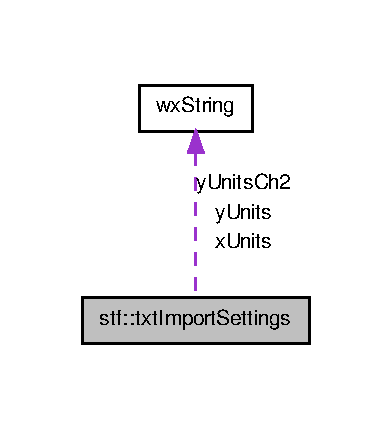
\includegraphics[width=188pt]{structstf_1_1txtImportSettings__coll__graph}
\end{center}
\end{figure}
\subsection*{Public Attributes}
\begin{DoxyCompactItemize}
\item 
int \hyperlink{structstf_1_1txtImportSettings_a7356008be84b96781c8dd98dac0c3dea}{hLines}
\item 
bool \hyperlink{structstf_1_1txtImportSettings_a5f475ef7099fe1cc9fb806b666a63459}{toSection}
\item 
bool \hyperlink{structstf_1_1txtImportSettings_af7123ba3b1732914e1f3009fc0ccb888}{firstIsTime}
\item 
int \hyperlink{structstf_1_1txtImportSettings_a7240de5e36d202c93f61ef4480dc3ae1}{ncolumns}
\item 
double \hyperlink{structstf_1_1txtImportSettings_a33e95b58e6cb81cd96c84ae89445f9be}{sr}
\item 
\hyperlink{classwxString}{wxString} \hyperlink{structstf_1_1txtImportSettings_a34394c27542cef2553d2c5b774fe31cd}{yUnits}
\item 
\hyperlink{classwxString}{wxString} \hyperlink{structstf_1_1txtImportSettings_abbc806479b71e4a566b0f997fe9ca006}{yUnitsCh2}
\item 
\hyperlink{classwxString}{wxString} \hyperlink{structstf_1_1txtImportSettings_aba0b71808e781ffff32bb560aa9a1d2a}{xUnits}
\end{DoxyCompactItemize}


\subsection{Detailed Description}
Text file import filter settings. 

\subsection{Member Data Documentation}
\hypertarget{structstf_1_1txtImportSettings_af7123ba3b1732914e1f3009fc0ccb888}{
\index{stf::txtImportSettings@{stf::txtImportSettings}!firstIsTime@{firstIsTime}}
\index{firstIsTime@{firstIsTime}!stf::txtImportSettings@{stf::txtImportSettings}}
\subsubsection[{firstIsTime}]{\setlength{\rightskip}{0pt plus 5cm}bool {\bf stf::txtImportSettings::firstIsTime}}}
\label{structstf_1_1txtImportSettings_af7123ba3b1732914e1f3009fc0ccb888}
First column contains time. \hypertarget{structstf_1_1txtImportSettings_a7356008be84b96781c8dd98dac0c3dea}{
\index{stf::txtImportSettings@{stf::txtImportSettings}!hLines@{hLines}}
\index{hLines@{hLines}!stf::txtImportSettings@{stf::txtImportSettings}}
\subsubsection[{hLines}]{\setlength{\rightskip}{0pt plus 5cm}int {\bf stf::txtImportSettings::hLines}}}
\label{structstf_1_1txtImportSettings_a7356008be84b96781c8dd98dac0c3dea}
Number of header lines. \hypertarget{structstf_1_1txtImportSettings_a7240de5e36d202c93f61ef4480dc3ae1}{
\index{stf::txtImportSettings@{stf::txtImportSettings}!ncolumns@{ncolumns}}
\index{ncolumns@{ncolumns}!stf::txtImportSettings@{stf::txtImportSettings}}
\subsubsection[{ncolumns}]{\setlength{\rightskip}{0pt plus 5cm}int {\bf stf::txtImportSettings::ncolumns}}}
\label{structstf_1_1txtImportSettings_a7240de5e36d202c93f61ef4480dc3ae1}
Number of columns. \hypertarget{structstf_1_1txtImportSettings_a33e95b58e6cb81cd96c84ae89445f9be}{
\index{stf::txtImportSettings@{stf::txtImportSettings}!sr@{sr}}
\index{sr@{sr}!stf::txtImportSettings@{stf::txtImportSettings}}
\subsubsection[{sr}]{\setlength{\rightskip}{0pt plus 5cm}double {\bf stf::txtImportSettings::sr}}}
\label{structstf_1_1txtImportSettings_a33e95b58e6cb81cd96c84ae89445f9be}
Sampling rate. \hypertarget{structstf_1_1txtImportSettings_a5f475ef7099fe1cc9fb806b666a63459}{
\index{stf::txtImportSettings@{stf::txtImportSettings}!toSection@{toSection}}
\index{toSection@{toSection}!stf::txtImportSettings@{stf::txtImportSettings}}
\subsubsection[{toSection}]{\setlength{\rightskip}{0pt plus 5cm}bool {\bf stf::txtImportSettings::toSection}}}
\label{structstf_1_1txtImportSettings_a5f475ef7099fe1cc9fb806b666a63459}
Import columns into separate sections rather than separate channels. \hypertarget{structstf_1_1txtImportSettings_aba0b71808e781ffff32bb560aa9a1d2a}{
\index{stf::txtImportSettings@{stf::txtImportSettings}!xUnits@{xUnits}}
\index{xUnits@{xUnits}!stf::txtImportSettings@{stf::txtImportSettings}}
\subsubsection[{xUnits}]{\setlength{\rightskip}{0pt plus 5cm}{\bf wxString} {\bf stf::txtImportSettings::xUnits}}}
\label{structstf_1_1txtImportSettings_aba0b71808e781ffff32bb560aa9a1d2a}
x units string. \hypertarget{structstf_1_1txtImportSettings_a34394c27542cef2553d2c5b774fe31cd}{
\index{stf::txtImportSettings@{stf::txtImportSettings}!yUnits@{yUnits}}
\index{yUnits@{yUnits}!stf::txtImportSettings@{stf::txtImportSettings}}
\subsubsection[{yUnits}]{\setlength{\rightskip}{0pt plus 5cm}{\bf wxString} {\bf stf::txtImportSettings::yUnits}}}
\label{structstf_1_1txtImportSettings_a34394c27542cef2553d2c5b774fe31cd}
y units string. \hypertarget{structstf_1_1txtImportSettings_abbc806479b71e4a566b0f997fe9ca006}{
\index{stf::txtImportSettings@{stf::txtImportSettings}!yUnitsCh2@{yUnitsCh2}}
\index{yUnitsCh2@{yUnitsCh2}!stf::txtImportSettings@{stf::txtImportSettings}}
\subsubsection[{yUnitsCh2}]{\setlength{\rightskip}{0pt plus 5cm}{\bf wxString} {\bf stf::txtImportSettings::yUnitsCh2}}}
\label{structstf_1_1txtImportSettings_abbc806479b71e4a566b0f997fe9ca006}
y units string of second channel. 

The documentation for this struct was generated from the following file:\begin{DoxyCompactItemize}
\item 
src/core/\hyperlink{stimdefs_8h}{stimdefs.h}\end{DoxyCompactItemize}

\hypertarget{structstf_1_1UserInput}{
\section{stf::UserInput Struct Reference}
\label{structstf_1_1UserInput}\index{stf::UserInput@{stf::UserInput}}
}


Represents user input from dialogs that can be used in plugins.  




{\ttfamily \#include $<$stimdefs.h$>$}



Collaboration diagram for stf::UserInput:
\nopagebreak
\begin{figure}[H]
\begin{center}
\leavevmode
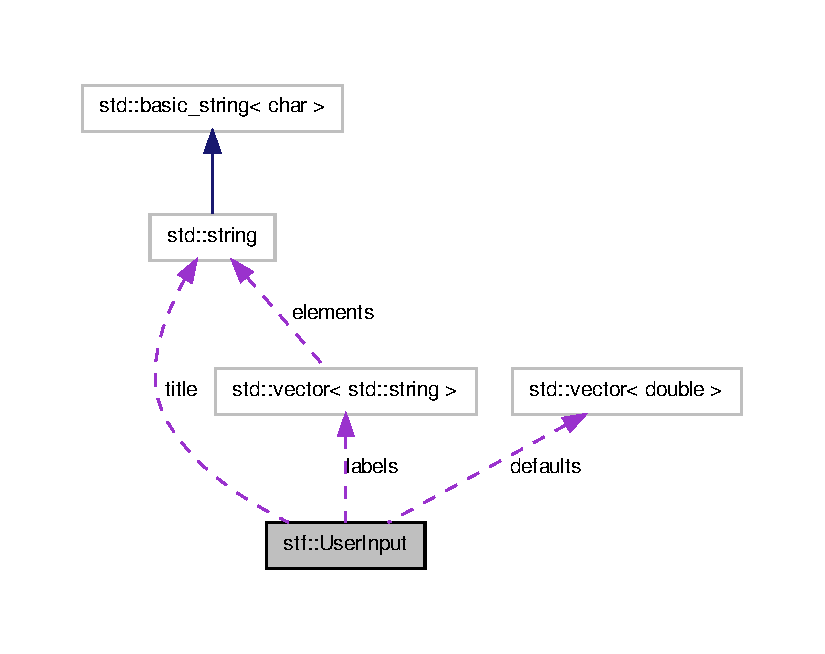
\includegraphics[width=396pt]{structstf_1_1UserInput__coll__graph}
\end{center}
\end{figure}
\subsection*{Public Member Functions}
\begin{DoxyCompactItemize}
\item 
\hyperlink{structstf_1_1UserInput_a879bc7b16a632a1079679fb0c42bb46e}{UserInput} (const std::vector$<$ std::string $>$ \&labels\_\-=std::vector$<$ std::string $>$(0), const Vector\_\-double \&defaults\_\-=Vector\_\-double(0), std::string title\_\-=\char`\"{}$\backslash$0\char`\"{})
\begin{DoxyCompactList}\small\item\em Constructor. \item\end{DoxyCompactList}\end{DoxyCompactItemize}
\subsection*{Public Attributes}
\begin{DoxyCompactItemize}
\item 
std::vector$<$ std::string $>$ \hyperlink{structstf_1_1UserInput_ab20fb35391b9c343150d61fe21e19461}{labels}
\item 
Vector\_\-double \hyperlink{structstf_1_1UserInput_a2ac332912f38c3ee90c5c18019ba49e0}{defaults}
\item 
std::string \hyperlink{structstf_1_1UserInput_abaae883a7067175ac27205bdfdc92d3f}{title}
\end{DoxyCompactItemize}


\subsection{Detailed Description}
Represents user input from dialogs that can be used in plugins. 

\subsection{Constructor \& Destructor Documentation}
\hypertarget{structstf_1_1UserInput_a879bc7b16a632a1079679fb0c42bb46e}{
\index{stf::UserInput@{stf::UserInput}!UserInput@{UserInput}}
\index{UserInput@{UserInput}!stf::UserInput@{stf::UserInput}}
\subsubsection[{UserInput}]{\setlength{\rightskip}{0pt plus 5cm}stf::UserInput::UserInput (
\begin{DoxyParamCaption}
\item[{const std::vector$<$ std::string $>$ \&}]{labels\_\- = {\ttfamily std::vector$<$std::string$>$(0)}, }
\item[{const Vector\_\-double \&}]{defaults\_\- = {\ttfamily Vector\_\-double(0)}, }
\item[{std::string}]{title\_\- = {\ttfamily \char`\"{}$\backslash$0\char`\"{}}}
\end{DoxyParamCaption}
)\hspace{0.3cm}{\ttfamily  \mbox{[}inline\mbox{]}}}}
\label{structstf_1_1UserInput_a879bc7b16a632a1079679fb0c42bb46e}


Constructor. 


\begin{DoxyParams}{Parameters}
{\em labels\_\-} & A vector of dialog entry label strings. \\
\hline
{\em defaults\_\-} & A vector of default dialog entries. \\
\hline
{\em title\_\-} & Dialog title. \\
\hline
\end{DoxyParams}


References defaults, and labels.



\subsection{Member Data Documentation}
\hypertarget{structstf_1_1UserInput_a2ac332912f38c3ee90c5c18019ba49e0}{
\index{stf::UserInput@{stf::UserInput}!defaults@{defaults}}
\index{defaults@{defaults}!stf::UserInput@{stf::UserInput}}
\subsubsection[{defaults}]{\setlength{\rightskip}{0pt plus 5cm}Vector\_\-double {\bf stf::UserInput::defaults}}}
\label{structstf_1_1UserInput_a2ac332912f38c3ee90c5c18019ba49e0}
Default dialog entries. 

Referenced by UserInput().

\hypertarget{structstf_1_1UserInput_ab20fb35391b9c343150d61fe21e19461}{
\index{stf::UserInput@{stf::UserInput}!labels@{labels}}
\index{labels@{labels}!stf::UserInput@{stf::UserInput}}
\subsubsection[{labels}]{\setlength{\rightskip}{0pt plus 5cm}std::vector$<$std::string$>$ {\bf stf::UserInput::labels}}}
\label{structstf_1_1UserInput_ab20fb35391b9c343150d61fe21e19461}
Dialog entry labels. 

Referenced by UserInput().

\hypertarget{structstf_1_1UserInput_abaae883a7067175ac27205bdfdc92d3f}{
\index{stf::UserInput@{stf::UserInput}!title@{title}}
\index{title@{title}!stf::UserInput@{stf::UserInput}}
\subsubsection[{title}]{\setlength{\rightskip}{0pt plus 5cm}std::string {\bf stf::UserInput::title}}}
\label{structstf_1_1UserInput_abaae883a7067175ac27205bdfdc92d3f}
Dialog title. 

The documentation for this struct was generated from the following file:\begin{DoxyCompactItemize}
\item 
src/core/\hyperlink{stimdefs_8h}{stimdefs.h}\end{DoxyCompactItemize}

\hypertarget{classwxApp}{
\section{wxApp Class Reference}
\label{classwxApp}\index{wxApp@{wxApp}}
}


See \href{http://www.wxwidgets.org/manuals/stable/wx_wxapp.html}{\tt http://www.wxwidgets.org/manuals/stable/wx\_\-wxapp.html} (wxWidgets documentation)  




{\ttfamily \#include $<$stimdefs.h$>$}



Inheritance diagram for wxApp:
\nopagebreak
\begin{figure}[H]
\begin{center}
\leavevmode
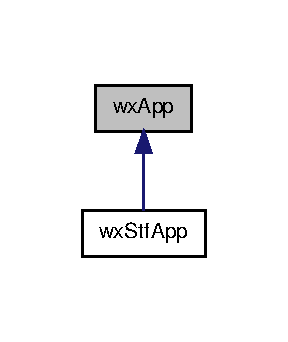
\includegraphics[width=138pt]{classwxApp__inherit__graph}
\end{center}
\end{figure}


\subsection{Detailed Description}
See \href{http://www.wxwidgets.org/manuals/stable/wx_wxapp.html}{\tt http://www.wxwidgets.org/manuals/stable/wx\_\-wxapp.html} (wxWidgets documentation) 

The documentation for this class was generated from the following file:\begin{DoxyCompactItemize}
\item 
src/core/\hyperlink{stimdefs_8h}{stimdefs.h}\end{DoxyCompactItemize}

\hypertarget{classwxCheckBox}{
\section{wxCheckBox Class Reference}
\label{classwxCheckBox}\index{wxCheckBox@{wxCheckBox}}
}


See \href{http://www.wxwidgets.org/manuals/stable/wx_wxcheckbox.html}{\tt http://www.wxwidgets.org/manuals/stable/wx\_\-wxcheckbox.html} (wxWidgets documentation)  




{\ttfamily \#include $<$stimdefs.h$>$}



Inheritance diagram for wxCheckBox:
\nopagebreak
\begin{figure}[H]
\begin{center}
\leavevmode
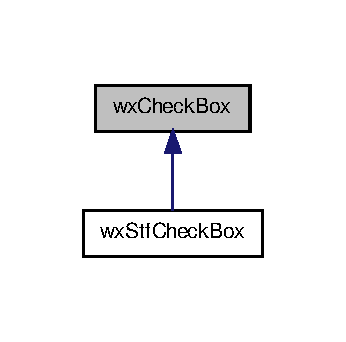
\includegraphics[width=166pt]{classwxCheckBox__inherit__graph}
\end{center}
\end{figure}


\subsection{Detailed Description}
See \href{http://www.wxwidgets.org/manuals/stable/wx_wxcheckbox.html}{\tt http://www.wxwidgets.org/manuals/stable/wx\_\-wxcheckbox.html} (wxWidgets documentation) 

The documentation for this class was generated from the following file:\begin{DoxyCompactItemize}
\item 
src/core/\hyperlink{stimdefs_8h}{stimdefs.h}\end{DoxyCompactItemize}

\hypertarget{classwxCommandEvent}{
\section{wxCommandEvent Class Reference}
\label{classwxCommandEvent}\index{wxCommandEvent@{wxCommandEvent}}
}


See \href{http://www.wxwidgets.org/manuals/stable/wx_wxcommandevent.html}{\tt http://www.wxwidgets.org/manuals/stable/wx\_\-wxcommandevent.html} (wxWidgets documentation)  




{\ttfamily \#include $<$stimdefs.h$>$}



\subsection{Detailed Description}
See \href{http://www.wxwidgets.org/manuals/stable/wx_wxcommandevent.html}{\tt http://www.wxwidgets.org/manuals/stable/wx\_\-wxcommandevent.html} (wxWidgets documentation) 

The documentation for this class was generated from the following file:\begin{DoxyCompactItemize}
\item 
src/core/\hyperlink{stimdefs_8h}{stimdefs.h}\end{DoxyCompactItemize}

\hypertarget{classwxDialog}{
\section{wxDialog Class Reference}
\label{classwxDialog}\index{wxDialog@{wxDialog}}
}


See \href{http://www.wxwidgets.org/manuals/stable/wx_wxdialog.html}{\tt http://www.wxwidgets.org/manuals/stable/wx\_\-wxdialog.html} (wxWidgets documentation)  




{\ttfamily \#include $<$stimdefs.h$>$}



Inheritance diagram for wxDialog:
\nopagebreak
\begin{figure}[H]
\begin{center}
\leavevmode
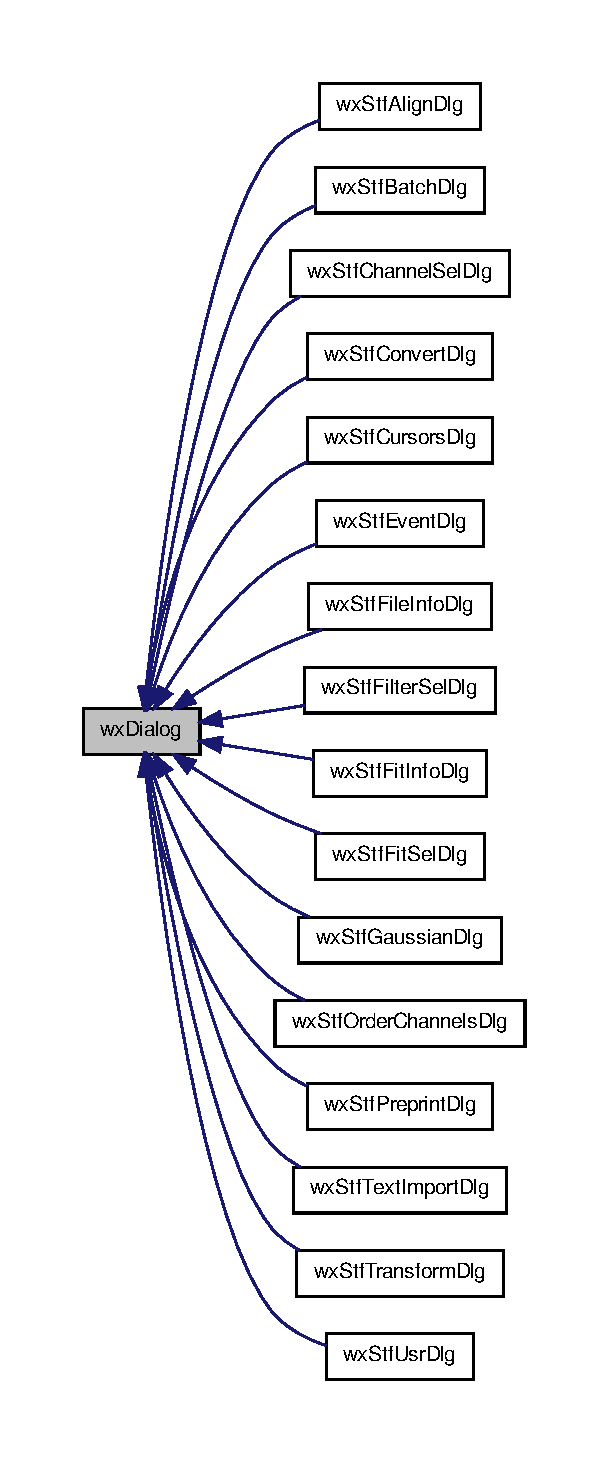
\includegraphics[height=600pt]{classwxDialog__inherit__graph}
\end{center}
\end{figure}


\subsection{Detailed Description}
See \href{http://www.wxwidgets.org/manuals/stable/wx_wxdialog.html}{\tt http://www.wxwidgets.org/manuals/stable/wx\_\-wxdialog.html} (wxWidgets documentation) 

The documentation for this class was generated from the following file:\begin{DoxyCompactItemize}
\item 
src/core/\hyperlink{stimdefs_8h}{stimdefs.h}\end{DoxyCompactItemize}

\hypertarget{classwxDocMDIChildFrame}{
\section{wxDocMDIChildFrame Class Reference}
\label{classwxDocMDIChildFrame}\index{wxDocMDIChildFrame@{wxDocMDIChildFrame}}
}


See \href{http://www.wxwidgets.org/manuals/stable/wx_wxdocmdichildframe.html}{\tt http://www.wxwidgets.org/manuals/stable/wx\_\-wxdocmdichildframe.html} (wxWidgets documentation)  




{\ttfamily \#include $<$stimdefs.h$>$}



Inheritance diagram for wxDocMDIChildFrame:
\nopagebreak
\begin{figure}[H]
\begin{center}
\leavevmode
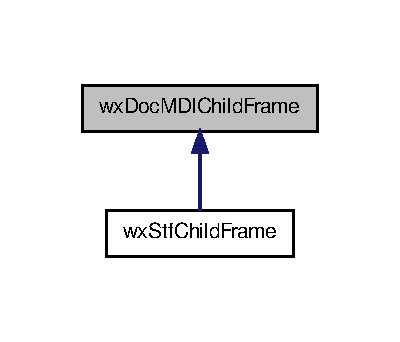
\includegraphics[width=192pt]{classwxDocMDIChildFrame__inherit__graph}
\end{center}
\end{figure}


\subsection{Detailed Description}
See \href{http://www.wxwidgets.org/manuals/stable/wx_wxdocmdichildframe.html}{\tt http://www.wxwidgets.org/manuals/stable/wx\_\-wxdocmdichildframe.html} (wxWidgets documentation) 

The documentation for this class was generated from the following file:\begin{DoxyCompactItemize}
\item 
src/core/\hyperlink{stimdefs_8h}{stimdefs.h}\end{DoxyCompactItemize}

\hypertarget{classwxDocMDIParentFrame}{
\section{wxDocMDIParentFrame Class Reference}
\label{classwxDocMDIParentFrame}\index{wxDocMDIParentFrame@{wxDocMDIParentFrame}}
}


See \href{http://www.wxwidgets.org/manuals/stable/wx_wxdocmdiparentframe.html}{\tt http://www.wxwidgets.org/manuals/stable/wx\_\-wxdocmdiparentframe.html} (wxWidgets documentation)  




{\ttfamily \#include $<$stimdefs.h$>$}



Inheritance diagram for wxDocMDIParentFrame:
\nopagebreak
\begin{figure}[H]
\begin{center}
\leavevmode
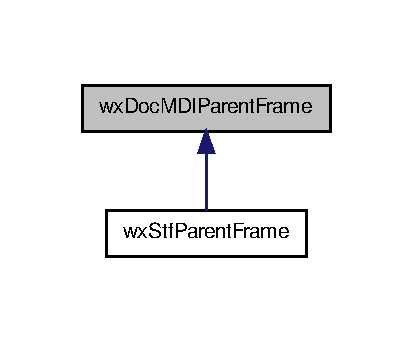
\includegraphics[width=198pt]{classwxDocMDIParentFrame__inherit__graph}
\end{center}
\end{figure}


\subsection{Detailed Description}
See \href{http://www.wxwidgets.org/manuals/stable/wx_wxdocmdiparentframe.html}{\tt http://www.wxwidgets.org/manuals/stable/wx\_\-wxdocmdiparentframe.html} (wxWidgets documentation) 

The documentation for this class was generated from the following file:\begin{DoxyCompactItemize}
\item 
src/core/\hyperlink{stimdefs_8h}{stimdefs.h}\end{DoxyCompactItemize}

\hypertarget{classwxDocument}{
\section{wxDocument Class Reference}
\label{classwxDocument}\index{wxDocument@{wxDocument}}
}


See \href{http://www.wxwidgets.org/manuals/stable/wx_wxdocument.html}{\tt http://www.wxwidgets.org/manuals/stable/wx\_\-wxdocument.html} (wxWidgets documentation)  




{\ttfamily \#include $<$stimdefs.h$>$}



Inheritance diagram for wxDocument:
\nopagebreak
\begin{figure}[H]
\begin{center}
\leavevmode
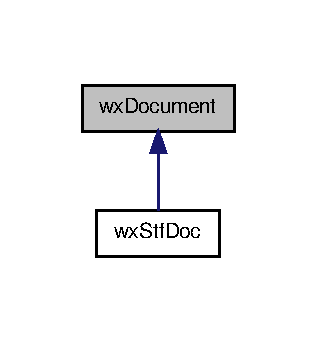
\includegraphics[width=152pt]{classwxDocument__inherit__graph}
\end{center}
\end{figure}


\subsection{Detailed Description}
See \href{http://www.wxwidgets.org/manuals/stable/wx_wxdocument.html}{\tt http://www.wxwidgets.org/manuals/stable/wx\_\-wxdocument.html} (wxWidgets documentation) 

The documentation for this class was generated from the following file:\begin{DoxyCompactItemize}
\item 
src/core/\hyperlink{stimdefs_8h}{stimdefs.h}\end{DoxyCompactItemize}

\hypertarget{classwxGrid}{
\section{wxGrid Class Reference}
\label{classwxGrid}\index{wxGrid@{wxGrid}}
}


See \href{http://www.wxwidgets.org/manuals/stable/wx_wxgrid.html}{\tt http://www.wxwidgets.org/manuals/stable/wx\_\-wxgrid.html} (wxWidgets documentation)  




{\ttfamily \#include $<$stimdefs.h$>$}



Inheritance diagram for wxGrid:
\nopagebreak
\begin{figure}[H]
\begin{center}
\leavevmode
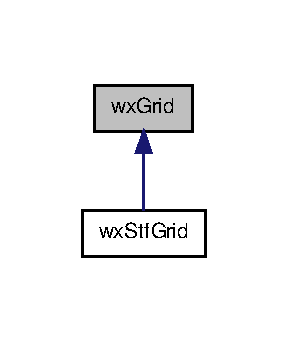
\includegraphics[width=138pt]{classwxGrid__inherit__graph}
\end{center}
\end{figure}


\subsection{Detailed Description}
See \href{http://www.wxwidgets.org/manuals/stable/wx_wxgrid.html}{\tt http://www.wxwidgets.org/manuals/stable/wx\_\-wxgrid.html} (wxWidgets documentation) 

The documentation for this class was generated from the following file:\begin{DoxyCompactItemize}
\item 
src/core/\hyperlink{stimdefs_8h}{stimdefs.h}\end{DoxyCompactItemize}

\hypertarget{classwxGridCellCoordsArray}{
\section{wxGridCellCoordsArray Class Reference}
\label{classwxGridCellCoordsArray}\index{wxGridCellCoordsArray@{wxGridCellCoordsArray}}
}


See \href{http://www.wxwidgets.org/manuals/stable/wx_wxgridcellcoordsarray.html}{\tt http://www.wxwidgets.org/manuals/stable/wx\_\-wxgridcellcoordsarray.html} (wxWidgets documentation)  




{\ttfamily \#include $<$stimdefs.h$>$}



\subsection{Detailed Description}
See \href{http://www.wxwidgets.org/manuals/stable/wx_wxgridcellcoordsarray.html}{\tt http://www.wxwidgets.org/manuals/stable/wx\_\-wxgridcellcoordsarray.html} (wxWidgets documentation) 

The documentation for this class was generated from the following file:\begin{DoxyCompactItemize}
\item 
src/core/\hyperlink{stimdefs_8h}{stimdefs.h}\end{DoxyCompactItemize}

\hypertarget{classwxGridTableBase}{
\section{wxGridTableBase Class Reference}
\label{classwxGridTableBase}\index{wxGridTableBase@{wxGridTableBase}}
}


See \href{http://www.wxwidgets.org/manuals/stable/wx_wxgridtablebase.html}{\tt http://www.wxwidgets.org/manuals/stable/wx\_\-wxgridtablebase.html} (wxWidgets documentation)  




{\ttfamily \#include $<$stimdefs.h$>$}



Inheritance diagram for wxGridTableBase:
\nopagebreak
\begin{figure}[H]
\begin{center}
\leavevmode
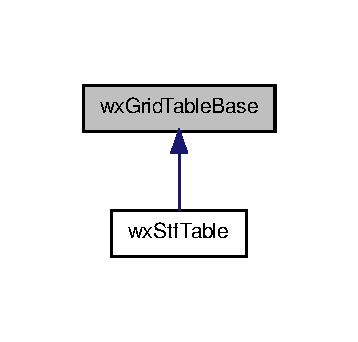
\includegraphics[width=172pt]{classwxGridTableBase__inherit__graph}
\end{center}
\end{figure}


\subsection{Detailed Description}
See \href{http://www.wxwidgets.org/manuals/stable/wx_wxgridtablebase.html}{\tt http://www.wxwidgets.org/manuals/stable/wx\_\-wxgridtablebase.html} (wxWidgets documentation) 

The documentation for this class was generated from the following file:\begin{DoxyCompactItemize}
\item 
src/core/\hyperlink{stimdefs_8h}{stimdefs.h}\end{DoxyCompactItemize}

\hypertarget{classwxPoint}{
\section{wxPoint Class Reference}
\label{classwxPoint}\index{wxPoint@{wxPoint}}
}


See \href{http://www.wxwidgets.org/manuals/stable/wx_wxpoint.html}{\tt http://www.wxwidgets.org/manuals/stable/wx\_\-wxpoint.html} (wxWidgets documentation)  




{\ttfamily \#include $<$stimdefs.h$>$}



\subsection{Detailed Description}
See \href{http://www.wxwidgets.org/manuals/stable/wx_wxpoint.html}{\tt http://www.wxwidgets.org/manuals/stable/wx\_\-wxpoint.html} (wxWidgets documentation) 

The documentation for this class was generated from the following file:\begin{DoxyCompactItemize}
\item 
src/core/\hyperlink{stimdefs_8h}{stimdefs.h}\end{DoxyCompactItemize}

\hypertarget{classwxPrintout}{
\section{wxPrintout Class Reference}
\label{classwxPrintout}\index{wxPrintout@{wxPrintout}}
}


See \href{http://www.wxwidgets.org/manuals/stable/wx_wxprintout.html}{\tt http://www.wxwidgets.org/manuals/stable/wx\_\-wxprintout.html} (wxWidgets documentation)  




{\ttfamily \#include $<$stimdefs.h$>$}



Inheritance diagram for wxPrintout:
\nopagebreak
\begin{figure}[H]
\begin{center}
\leavevmode
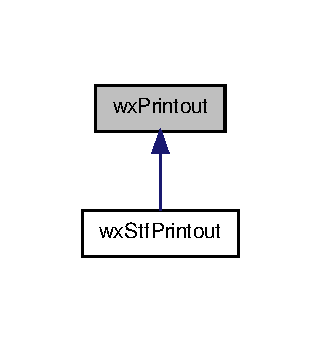
\includegraphics[width=154pt]{classwxPrintout__inherit__graph}
\end{center}
\end{figure}


\subsection{Detailed Description}
See \href{http://www.wxwidgets.org/manuals/stable/wx_wxprintout.html}{\tt http://www.wxwidgets.org/manuals/stable/wx\_\-wxprintout.html} (wxWidgets documentation) 

The documentation for this class was generated from the following file:\begin{DoxyCompactItemize}
\item 
src/core/\hyperlink{stimdefs_8h}{stimdefs.h}\end{DoxyCompactItemize}

\hypertarget{classwxSize}{
\section{wxSize Class Reference}
\label{classwxSize}\index{wxSize@{wxSize}}
}


See \href{http://www.wxwidgets.org/manuals/stable/wx_wxsize.html}{\tt http://www.wxwidgets.org/manuals/stable/wx\_\-wxsize.html} (wxWidgets documentation)  




{\ttfamily \#include $<$stimdefs.h$>$}



\subsection{Detailed Description}
See \href{http://www.wxwidgets.org/manuals/stable/wx_wxsize.html}{\tt http://www.wxwidgets.org/manuals/stable/wx\_\-wxsize.html} (wxWidgets documentation) 

The documentation for this class was generated from the following file:\begin{DoxyCompactItemize}
\item 
src/core/\hyperlink{stimdefs_8h}{stimdefs.h}\end{DoxyCompactItemize}

\hypertarget{classwxStfAlignDlg}{
\section{wxStfAlignDlg Class Reference}
\label{classwxStfAlignDlg}\index{wxStfAlignDlg@{wxStfAlignDlg}}
}


Dialog for selecting alignment mode.  




{\ttfamily \#include $<$smalldlgs.h$>$}



Inheritance diagram for wxStfAlignDlg:
\nopagebreak
\begin{figure}[H]
\begin{center}
\leavevmode
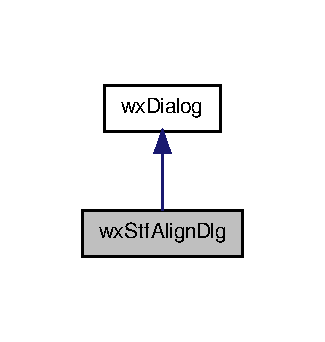
\includegraphics[width=156pt]{classwxStfAlignDlg__inherit__graph}
\end{center}
\end{figure}


Collaboration diagram for wxStfAlignDlg:
\nopagebreak
\begin{figure}[H]
\begin{center}
\leavevmode
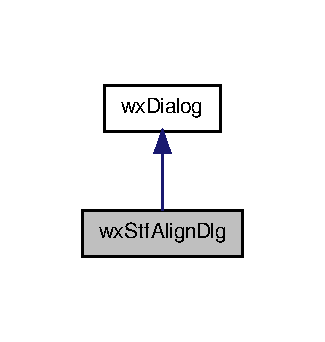
\includegraphics[width=156pt]{classwxStfAlignDlg__coll__graph}
\end{center}
\end{figure}
\subsection*{Public Member Functions}
\begin{DoxyCompactItemize}
\item 
\hyperlink{classwxStfAlignDlg_a91fcede6329a5707fa63575f44f46d8d}{wxStfAlignDlg} (\hyperlink{classwxWindow}{wxWindow} $\ast$parent, int id=wxID\_\-ANY, \hyperlink{classwxString}{wxString} title=wxT(\char`\"{}Alignment mode\char`\"{}), wxPoint pos=wxDefaultPosition, \hyperlink{classwxSize}{wxSize} size=wxDefaultSize, int style=wxCAPTION)
\begin{DoxyCompactList}\small\item\em Constructor. \item\end{DoxyCompactList}\item 
bool \hyperlink{classwxStfAlignDlg_af63c6dfa13c434175a37c965c4d7bdc5}{AlignRise} () const 
\begin{DoxyCompactList}\small\item\em Indicates whether the average should be aligned to the steepest rise. \item\end{DoxyCompactList}\item 
virtual void \hyperlink{classwxStfAlignDlg_a385cdd58c4f99b5a2ec7917dc5ac5877}{EndModal} (int retCode)
\begin{DoxyCompactList}\small\item\em Called upon ending a modal dialog. \item\end{DoxyCompactList}\end{DoxyCompactItemize}


\subsection{Detailed Description}
Dialog for selecting alignment mode. 

\subsection{Constructor \& Destructor Documentation}
\hypertarget{classwxStfAlignDlg_a91fcede6329a5707fa63575f44f46d8d}{
\index{wxStfAlignDlg@{wxStfAlignDlg}!wxStfAlignDlg@{wxStfAlignDlg}}
\index{wxStfAlignDlg@{wxStfAlignDlg}!wxStfAlignDlg@{wxStfAlignDlg}}
\subsubsection[{wxStfAlignDlg}]{\setlength{\rightskip}{0pt plus 5cm}wxStfAlignDlg::wxStfAlignDlg (
\begin{DoxyParamCaption}
\item[{{\bf wxWindow} $\ast$}]{parent, }
\item[{int}]{id = {\ttfamily wxID\_\-ANY}, }
\item[{{\bf wxString}}]{title = {\ttfamily wxT(\char`\"{}Alignment~mode\char`\"{})}, }
\item[{{\bf wxPoint}}]{pos = {\ttfamily wxDefaultPosition}, }
\item[{{\bf wxSize}}]{size = {\ttfamily wxDefaultSize}, }
\item[{int}]{style = {\ttfamily wxCAPTION}}
\end{DoxyParamCaption}
)}}
\label{classwxStfAlignDlg_a91fcede6329a5707fa63575f44f46d8d}


Constructor. 


\begin{DoxyParams}{Parameters}
{\em parent} & Pointer to parent window. \\
\hline
{\em id} & Window id. \\
\hline
{\em title} & Dialog title. \\
\hline
{\em pos} & Initial position. \\
\hline
{\em size} & Initial size. \\
\hline
{\em style} & Dialog style. \\
\hline
\end{DoxyParams}


\subsection{Member Function Documentation}
\hypertarget{classwxStfAlignDlg_af63c6dfa13c434175a37c965c4d7bdc5}{
\index{wxStfAlignDlg@{wxStfAlignDlg}!AlignRise@{AlignRise}}
\index{AlignRise@{AlignRise}!wxStfAlignDlg@{wxStfAlignDlg}}
\subsubsection[{AlignRise}]{\setlength{\rightskip}{0pt plus 5cm}bool wxStfAlignDlg::AlignRise (
\begin{DoxyParamCaption}
{}
\end{DoxyParamCaption}
) const\hspace{0.3cm}{\ttfamily  \mbox{[}inline\mbox{]}}}}
\label{classwxStfAlignDlg_af63c6dfa13c434175a37c965c4d7bdc5}


Indicates whether the average should be aligned to the steepest rise. 

\begin{DoxyReturn}{Returns}
true if it should be aligned to the steepest rise, false if it should be aligned to the peak. 
\end{DoxyReturn}
\hypertarget{classwxStfAlignDlg_a385cdd58c4f99b5a2ec7917dc5ac5877}{
\index{wxStfAlignDlg@{wxStfAlignDlg}!EndModal@{EndModal}}
\index{EndModal@{EndModal}!wxStfAlignDlg@{wxStfAlignDlg}}
\subsubsection[{EndModal}]{\setlength{\rightskip}{0pt plus 5cm}virtual void wxStfAlignDlg::EndModal (
\begin{DoxyParamCaption}
\item[{int}]{retCode}
\end{DoxyParamCaption}
)\hspace{0.3cm}{\ttfamily  \mbox{[}virtual\mbox{]}}}}
\label{classwxStfAlignDlg_a385cdd58c4f99b5a2ec7917dc5ac5877}


Called upon ending a modal dialog. 


\begin{DoxyParams}{Parameters}
{\em retCode} & The dialog button id that ended the dialog (e.g. wxID\_\-OK) \\
\hline
\end{DoxyParams}


The documentation for this class was generated from the following file:\begin{DoxyCompactItemize}
\item 
src/app/dlgs/\hyperlink{smalldlgs_8h}{smalldlgs.h}\end{DoxyCompactItemize}

\hypertarget{classwxStfApp}{
\section{wxStfApp Class Reference}
\label{classwxStfApp}\index{wxStfApp@{wxStfApp}}
}


The application, derived from \hyperlink{classwxApp}{wxApp}.  




{\ttfamily \#include $<$app.h$>$}



Inheritance diagram for wxStfApp:
\nopagebreak
\begin{figure}[H]
\begin{center}
\leavevmode
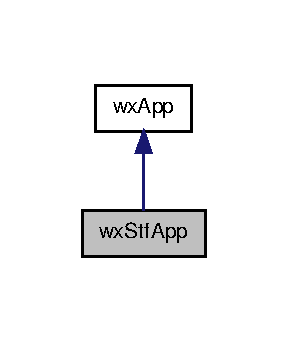
\includegraphics[width=138pt]{classwxStfApp__inherit__graph}
\end{center}
\end{figure}


Collaboration diagram for wxStfApp:
\nopagebreak
\begin{figure}[H]
\begin{center}
\leavevmode
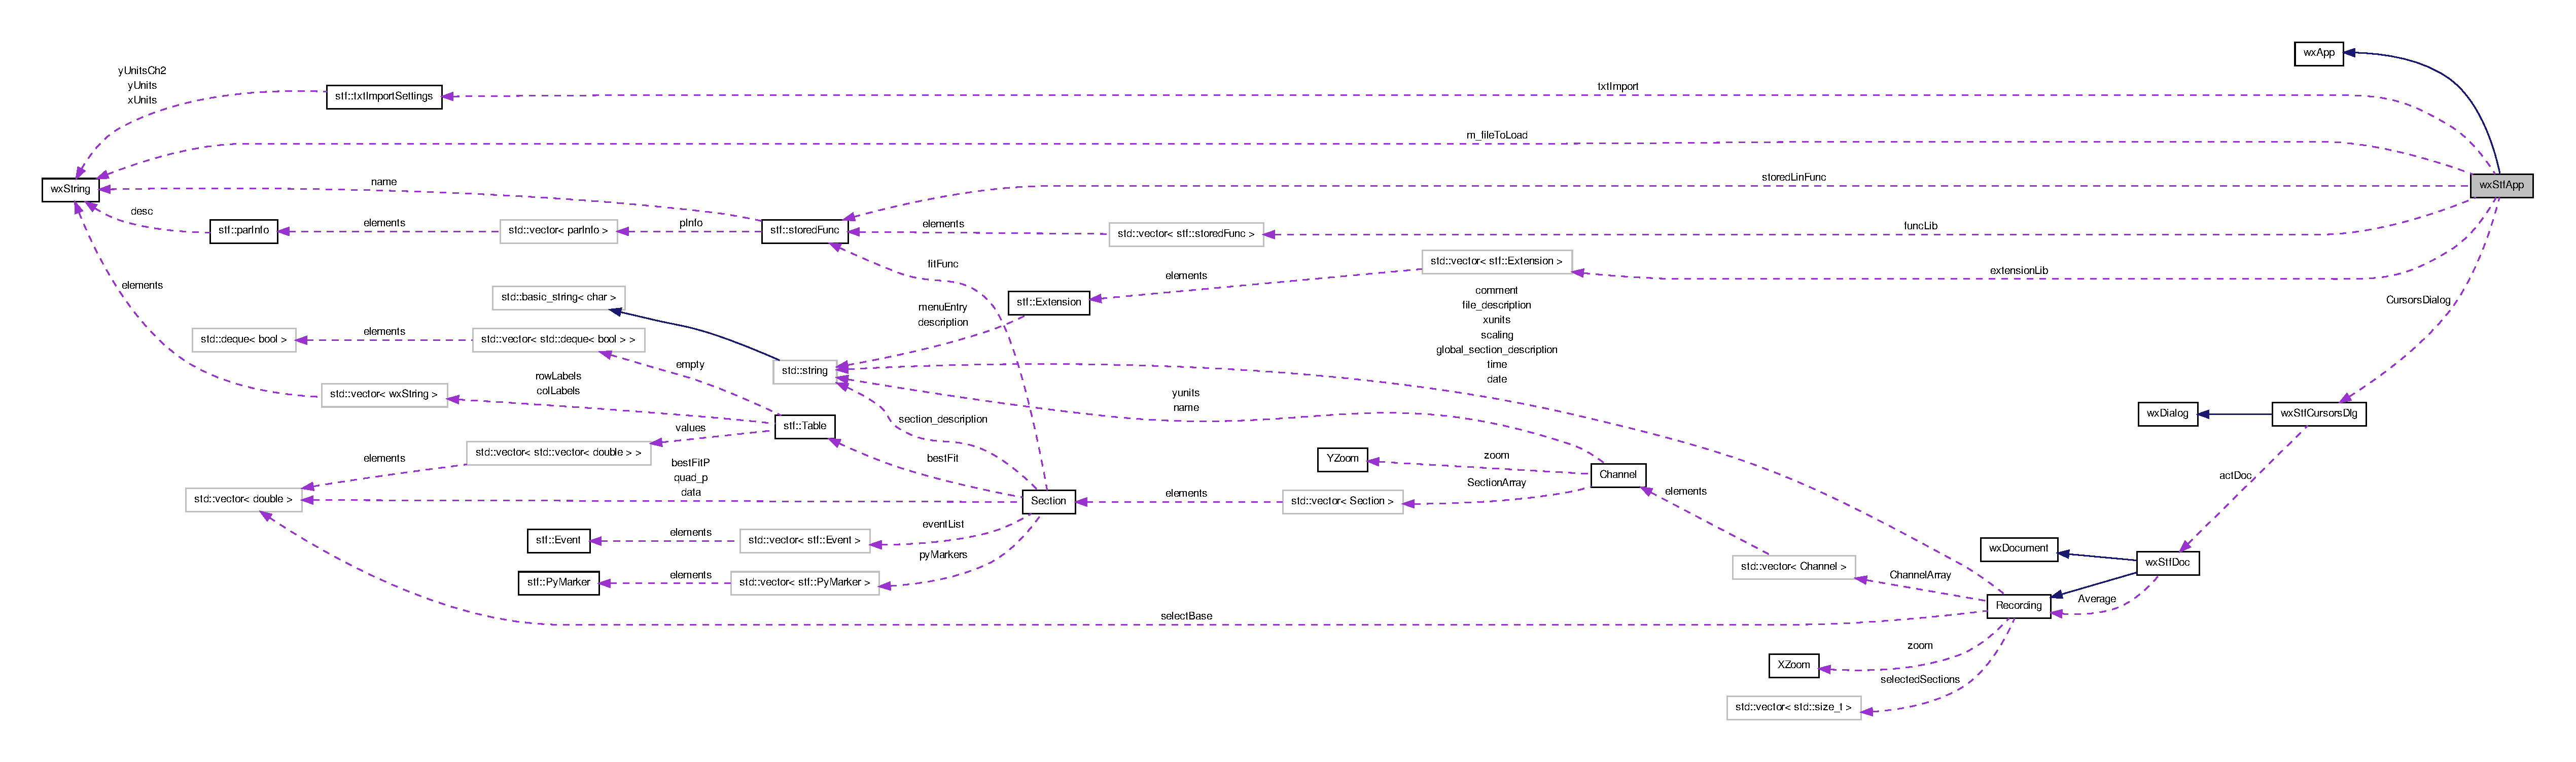
\includegraphics[width=400pt]{classwxStfApp__coll__graph}
\end{center}
\end{figure}
\subsection*{Public Member Functions}
\begin{DoxyCompactItemize}
\item 
\hypertarget{classwxStfApp_a589012f57e32c0c45fda2db4f88d93bb}{
\hyperlink{classwxStfApp_a589012f57e32c0c45fda2db4f88d93bb}{wxStfApp} ()}
\label{classwxStfApp_a589012f57e32c0c45fda2db4f88d93bb}

\begin{DoxyCompactList}\small\item\em Constructor. \item\end{DoxyCompactList}\item 
virtual bool \hyperlink{classwxStfApp_a2933498655e65fab015ccc643f97e096}{OnInit} ()
\begin{DoxyCompactList}\small\item\em Initialise the application. \item\end{DoxyCompactList}\item 
virtual int \hyperlink{classwxStfApp_ad0777eb76fe6a4b73ac95e41eefe7768}{OnExit} ()
\begin{DoxyCompactList}\small\item\em Exit the application. \item\end{DoxyCompactList}\item 
\hyperlink{classwxStfChildFrame}{wxStfChildFrame} $\ast$ \hyperlink{classwxStfApp_a3e1a978b7ade905d5ee2465305273b88}{CreateChildFrame} (\hyperlink{classwxDocument}{wxDocument} $\ast$doc, \hyperlink{classwxView}{wxView} $\ast$view)
\begin{DoxyCompactList}\small\item\em Creates a new child frame. \item\end{DoxyCompactList}\item 
\hyperlink{classwxStfDoc}{wxStfDoc} $\ast$ \hyperlink{classwxStfApp_a1300dc5dad0790f58726e11088441b18}{GetActiveDoc} () const 
\begin{DoxyCompactList}\small\item\em Retrieves the currently active document. \item\end{DoxyCompactList}\item 
\hyperlink{classwxStfView}{wxStfView} $\ast$ \hyperlink{classwxStfApp_a62a9c9d666190a4389224686b6dd7faa}{GetActiveView} () const 
\begin{DoxyCompactList}\small\item\em Sets the currently active document. \item\end{DoxyCompactList}\item 
void \hyperlink{classwxStfApp_a4d1d4887f607e088a871b42b6a878bdd}{ErrorMsg} (const \hyperlink{classwxString}{wxString} \&msg) const 
\begin{DoxyCompactList}\small\item\em Displays a message box when an error has occured. \item\end{DoxyCompactList}\item 
void \hyperlink{classwxStfApp_a37646b2722c97ff92abeaecb9b9e7198}{ExceptMsg} (const \hyperlink{classwxString}{wxString} \&msg) const 
\begin{DoxyCompactList}\small\item\em Displays a message box when an exception has occured. \item\end{DoxyCompactList}\item 
void \hyperlink{classwxStfApp_ab18bb61cbd01df81e8577494ed1221a5}{InfoMsg} (const \hyperlink{classwxString}{wxString} \&msg) const 
\begin{DoxyCompactList}\small\item\em Displays a message box with information. \item\end{DoxyCompactList}\item 
bool \hyperlink{classwxStfApp_a2ba47fb8c9f58b21211fbfb915c46a80}{get\_\-directTxtImport} () const 
\begin{DoxyCompactList}\small\item\em Indicates whether text files should be imported directly without showing an import settings dialog. \item\end{DoxyCompactList}\item 
void \hyperlink{classwxStfApp_aa00f88aecbfd73fa18a0141fe42bc879}{set\_\-directTxtImport} (bool directTxtImport\_\-)
\begin{DoxyCompactList}\small\item\em Determines whether text files should be imported directly without showing an import filter settings dialog. \item\end{DoxyCompactList}\item 
const \hyperlink{structstf_1_1txtImportSettings}{stf::txtImportSettings} \& \hyperlink{classwxStfApp_af7fcc335ab5df92c0df0eeb846d22476}{GetTxtImport} () const 
\begin{DoxyCompactList}\small\item\em Retrieves the text import filter settings. \item\end{DoxyCompactList}\item 
void \hyperlink{classwxStfApp_a6f94ead9d8e03baf99d3deec56582920}{set\_\-txtImportSettings} (const \hyperlink{structstf_1_1txtImportSettings}{stf::txtImportSettings} \&txtImport\_\-)
\begin{DoxyCompactList}\small\item\em Sets the text import filter settings. \item\end{DoxyCompactList}\item 
const std::vector$<$ \hyperlink{structstf_1_1storedFunc}{stf::storedFunc} $>$ \& \hyperlink{classwxStfApp_aa46d93e619d2698aa807390c51980f3e}{GetFuncLib} () const 
\begin{DoxyCompactList}\small\item\em Retrieves the functions that are available for least-\/squares minimisation. \item\end{DoxyCompactList}\item 
\hyperlink{structstf_1_1storedFunc}{stf::storedFunc} $\ast$ \hyperlink{classwxStfApp_a68cc63c9e6d555e364f6ac175e27016e}{GetFuncLibPtr} (std::size\_\-t at)
\begin{DoxyCompactList}\small\item\em Retrieves a pointer to a function for least-\/squares minimisation. \item\end{DoxyCompactList}\item 
\hyperlink{structstf_1_1storedFunc}{stf::storedFunc} $\ast$ \hyperlink{classwxStfApp_a9d5cbe83f3a3329c3649c3374004b87f}{GetLinFuncPtr} ()
\begin{DoxyCompactList}\small\item\em Retrieves a pointer to a function for least-\/squares minimisation. \item\end{DoxyCompactList}\item 
const std::vector$<$ \hyperlink{structstf_1_1Extension}{stf::Extension} $>$ \& \hyperlink{classwxStfApp_a29f0f699a0545eb4ae8219ec83c4aa0a}{GetExtensionLib} () const 
\begin{DoxyCompactList}\small\item\em Retrieves the user-\/defined extension functions. \item\end{DoxyCompactList}\item 
\hyperlink{classwxStfCursorsDlg}{wxStfCursorsDlg} $\ast$ \hyperlink{classwxStfApp_ac953818454f409adebdc2a195225c292}{GetCursorsDialog} () const 
\begin{DoxyCompactList}\small\item\em Retrieves the cursor settings dialog. \item\end{DoxyCompactList}\item 
std::vector$<$ \hyperlink{classSection}{Section} $\ast$ $>$ \hyperlink{classwxStfApp_a2b27b151af8a1062542f35c466281b55}{GetSectionsWithFits} () const 
\begin{DoxyCompactList}\small\item\em Retrieves all sections with fits. \item\end{DoxyCompactList}\item 
void \hyperlink{classwxStfApp_a487f19baf697d6e51db9c3a4f27cacf6}{wxWriteProfileInt} (const \hyperlink{classwxString}{wxString} \&main, const \hyperlink{classwxString}{wxString} \&sub, int value) const 
\begin{DoxyCompactList}\small\item\em Writes an integer value to the configuration. \item\end{DoxyCompactList}\item 
int \hyperlink{classwxStfApp_a2fa40721aba5a795665a99711701b3b0}{wxGetProfileInt} (const \hyperlink{classwxString}{wxString} \&main, const \hyperlink{classwxString}{wxString} \&sub, int default\_\-) const 
\begin{DoxyCompactList}\small\item\em Retrieves an integer value from the configuration. \item\end{DoxyCompactList}\item 
void \hyperlink{classwxStfApp_a731ce695f19f790f9e5b49252c3cddeb}{wxWriteProfileString} (const \hyperlink{classwxString}{wxString} \&main, const \hyperlink{classwxString}{wxString} \&sub, const \hyperlink{classwxString}{wxString} \&value) const 
\begin{DoxyCompactList}\small\item\em Writes a string to the configuration. \item\end{DoxyCompactList}\item 
\hyperlink{classwxString}{wxString} \hyperlink{classwxStfApp_a509da5804564d52e34d87a77f43c4aa7}{wxGetProfileString} (const \hyperlink{classwxString}{wxString} \&main, const \hyperlink{classwxString}{wxString} \&sub, const \hyperlink{classwxString}{wxString} \&default\_\-) const 
\begin{DoxyCompactList}\small\item\em Retrieves a string from the configuration. \item\end{DoxyCompactList}\item 
\hyperlink{classwxStfDoc}{wxStfDoc} $\ast$ \hyperlink{classwxStfApp_ac38d9f10644fef847d50cfac42353c38}{NewChild} (const \hyperlink{classRecording}{Recording} \&NewData, const \hyperlink{classwxStfDoc}{wxStfDoc} $\ast$Sender, const \hyperlink{classwxString}{wxString} \&title=wxT(\char`\"{}$\backslash$0\char`\"{}))
\begin{DoxyCompactList}\small\item\em Creates a new child window showing a new document. \item\end{DoxyCompactList}\item 
void \hyperlink{classwxStfApp_a584396d82492d98d08c74689a1adfbc3}{OnPeakcalcexecMsg} (\hyperlink{classwxStfDoc}{wxStfDoc} $\ast$actDoc=0)
\begin{DoxyCompactList}\small\item\em Execute all pending calculations. \item\end{DoxyCompactList}\item 
void \hyperlink{classwxStfApp_aad9c9b808e1568f9f4e4266be1e7c7b9}{CleanupDocument} (\hyperlink{classwxStfDoc}{wxStfDoc} $\ast$pDoc)
\begin{DoxyCompactList}\small\item\em Destroys the last cursor settings dialog when the last document is closed. \item\end{DoxyCompactList}\item 
\hypertarget{classwxStfApp_a7a112fcc6db87597de9adcc8987c6355}{
bool \hyperlink{classwxStfApp_a7a112fcc6db87597de9adcc8987c6355}{CloseAll} ()}
\label{classwxStfApp_a7a112fcc6db87597de9adcc8987c6355}

\begin{DoxyCompactList}\small\item\em Closes all documents. \item\end{DoxyCompactList}\item 
bool \hyperlink{classwxStfApp_ae091bc0de048b5386379f934a71f3d20}{OpenFileSeries} (const wxArrayString \&fNameArray)
\begin{DoxyCompactList}\small\item\em Opens a series of files. Optionally, files can be put into a single window. \item\end{DoxyCompactList}\item 
int \hyperlink{classwxStfApp_a09fd899d6efaca715f7e22dd1ddb3ccf}{GetDocCount} ()
\begin{DoxyCompactList}\small\item\em Returns the number of currently opened documents. \item\end{DoxyCompactList}\item 
void \hyperlink{classwxStfApp_a876a3f37ff3cd08ac00fa4ef6b1b2c5d}{set\_\-isBars} (bool value)
\begin{DoxyCompactList}\small\item\em Determine whether scale bars or coordinates should be shown. \item\end{DoxyCompactList}\item 
bool \hyperlink{classwxStfApp_a2d731c3c77d94fe13ad8184fa1f5cb5f}{get\_\-isBars} () const 
\begin{DoxyCompactList}\small\item\em Indicates whether scale bars or coordinates are shown. \item\end{DoxyCompactList}\item 
void \hyperlink{classwxStfApp_a19263b9dec3c8506d801c3becada2a18}{set\_\-isHires} (bool value)
\begin{DoxyCompactList}\small\item\em Determine whether a high or a low resolution should be used for drawing traces. \item\end{DoxyCompactList}\item 
bool \hyperlink{classwxStfApp_a73345a1fd9b9f33f5aaf8d7f5a2c1df3}{get\_\-isHires} () const 
\begin{DoxyCompactList}\small\item\em Indicates whether a high or a low resolution is used for drawing traces. \item\end{DoxyCompactList}\item 
\hyperlink{classwxString}{wxString} \hyperlink{classwxStfApp_a3e2dfcb798c3451a31b84ec712ae52fd}{GetVersionString} () const 
\begin{DoxyCompactList}\small\item\em Get a formatted version string. \item\end{DoxyCompactList}\item 
void \hyperlink{classwxStfApp_ad84ab3a7bc030ba2b1a03924f8e90386}{OnNewfromselected} (\hyperlink{classwxCommandEvent}{wxCommandEvent} \&event)
\begin{DoxyCompactList}\small\item\em Open a new window showing all selected traces from all open files. \item\end{DoxyCompactList}\item 
wxDocManager $\ast$ \hyperlink{classwxStfApp_a5fad31f2760593bec972912461e2e2e4}{GetDocManager} () const 
\begin{DoxyCompactList}\small\item\em Access the document manager. \item\end{DoxyCompactList}\item 
\hypertarget{classwxStfApp_a6a012628e86f748873c91ab039373fc8}{
virtual void {\bfseries OnInitCmdLine} (wxCmdLineParser \&parser)}
\label{classwxStfApp_a6a012628e86f748873c91ab039373fc8}

\item 
\hypertarget{classwxStfApp_a6bbcf577566590abb524e842692688c3}{
virtual bool {\bfseries OnCmdLineParsed} (wxCmdLineParser \&parser)}
\label{classwxStfApp_a6bbcf577566590abb524e842692688c3}

\item 
bool \hyperlink{classwxStfApp_ad8c1479a2b4e101482005d2cbae660bf}{OpenFilePy} (const \hyperlink{classwxString}{wxString} \&fNameArray)
\begin{DoxyCompactList}\small\item\em Opens a file in a new window, to be called from Python. \item\end{DoxyCompactList}\item 
void \hyperlink{classwxStfApp_aa5887b87ba6889cffc3c77b4f4b97b8c}{OnPythonImport} (\hyperlink{classwxCommandEvent}{wxCommandEvent} \&event)
\begin{DoxyCompactList}\small\item\em Opens a dialog to import a Python module. \item\end{DoxyCompactList}\end{DoxyCompactItemize}


\subsection{Detailed Description}
The application, derived from \hyperlink{classwxApp}{wxApp}. This class is used to set and get application-\/wide properties, implement the windowing system message or event loop, initiate application processing via OnInit, and allow default processing of events not handled by other objects in the application. 

\subsection{Member Function Documentation}
\hypertarget{classwxStfApp_aad9c9b808e1568f9f4e4266be1e7c7b9}{
\index{wxStfApp@{wxStfApp}!CleanupDocument@{CleanupDocument}}
\index{CleanupDocument@{CleanupDocument}!wxStfApp@{wxStfApp}}
\subsubsection[{CleanupDocument}]{\setlength{\rightskip}{0pt plus 5cm}void wxStfApp::CleanupDocument (
\begin{DoxyParamCaption}
\item[{{\bf wxStfDoc} $\ast$}]{pDoc}
\end{DoxyParamCaption}
)}}
\label{classwxStfApp_aad9c9b808e1568f9f4e4266be1e7c7b9}


Destroys the last cursor settings dialog when the last document is closed. 

Do not use this function directly. It only needs to be called from \hyperlink{classwxStfDoc_aeb6ac6149de1d6f580bde0d220810d2d}{wxStfDoc::OnCloseDocument()}. 
\begin{DoxyParams}{Parameters}
{\em pDoc} & Pointer to the document that is being closed. \\
\hline
\end{DoxyParams}
\hypertarget{classwxStfApp_a3e1a978b7ade905d5ee2465305273b88}{
\index{wxStfApp@{wxStfApp}!CreateChildFrame@{CreateChildFrame}}
\index{CreateChildFrame@{CreateChildFrame}!wxStfApp@{wxStfApp}}
\subsubsection[{CreateChildFrame}]{\setlength{\rightskip}{0pt plus 5cm}{\bf wxStfChildFrame}$\ast$ wxStfApp::CreateChildFrame (
\begin{DoxyParamCaption}
\item[{{\bf wxDocument} $\ast$}]{doc, }
\item[{{\bf wxView} $\ast$}]{view}
\end{DoxyParamCaption}
)}}
\label{classwxStfApp_a3e1a978b7ade905d5ee2465305273b88}


Creates a new child frame. 

This is called from view.cpp whenever a child frame is created. If you want to pop up a new frame showing a new document, use \hyperlink{classwxStfApp_ac38d9f10644fef847d50cfac42353c38}{NewChild()} instead; this function will then be called by the newly created view. 
\begin{DoxyParams}{Parameters}
{\em doc} & A pointer to the document that the new child frame should contain. \\
\hline
{\em view} & A pointer to the view corresponding to the document. \\
\hline
\end{DoxyParams}
\begin{DoxyReturn}{Returns}
A pointer to the newly created child frame. 
\end{DoxyReturn}
\hypertarget{classwxStfApp_a4d1d4887f607e088a871b42b6a878bdd}{
\index{wxStfApp@{wxStfApp}!ErrorMsg@{ErrorMsg}}
\index{ErrorMsg@{ErrorMsg}!wxStfApp@{wxStfApp}}
\subsubsection[{ErrorMsg}]{\setlength{\rightskip}{0pt plus 5cm}void wxStfApp::ErrorMsg (
\begin{DoxyParamCaption}
\item[{const {\bf wxString} \&}]{msg}
\end{DoxyParamCaption}
) const\hspace{0.3cm}{\ttfamily  \mbox{[}inline\mbox{]}}}}
\label{classwxStfApp_a4d1d4887f607e088a871b42b6a878bdd}


Displays a message box when an error has occured. 

You can use this function from almost anywhere using \hyperlink{group__wxstf_ga10919857dea79326b815ec8555077e07}{wxGetApp()}.ErrorMsg( wxT( \char`\"{}Error abc: xyz\char`\"{} ) ); 
\begin{DoxyParams}{Parameters}
{\em msg} & The message string to be shown. \\
\hline
\end{DoxyParams}
\hypertarget{classwxStfApp_a37646b2722c97ff92abeaecb9b9e7198}{
\index{wxStfApp@{wxStfApp}!ExceptMsg@{ExceptMsg}}
\index{ExceptMsg@{ExceptMsg}!wxStfApp@{wxStfApp}}
\subsubsection[{ExceptMsg}]{\setlength{\rightskip}{0pt plus 5cm}void wxStfApp::ExceptMsg (
\begin{DoxyParamCaption}
\item[{const {\bf wxString} \&}]{msg}
\end{DoxyParamCaption}
) const\hspace{0.3cm}{\ttfamily  \mbox{[}inline\mbox{]}}}}
\label{classwxStfApp_a37646b2722c97ff92abeaecb9b9e7198}


Displays a message box when an exception has occured. 

You can use this function from almost anywhere using \hyperlink{group__wxstf_ga10919857dea79326b815ec8555077e07}{wxGetApp()}.ExceptMsg( wxT( \char`\"{}Exception description xyz\char`\"{} ) ); 
\begin{DoxyParams}{Parameters}
{\em msg} & The message string to be shown. \\
\hline
\end{DoxyParams}
\hypertarget{classwxStfApp_a2ba47fb8c9f58b21211fbfb915c46a80}{
\index{wxStfApp@{wxStfApp}!get\_\-directTxtImport@{get\_\-directTxtImport}}
\index{get\_\-directTxtImport@{get\_\-directTxtImport}!wxStfApp@{wxStfApp}}
\subsubsection[{get\_\-directTxtImport}]{\setlength{\rightskip}{0pt plus 5cm}bool wxStfApp::get\_\-directTxtImport (
\begin{DoxyParamCaption}
{}
\end{DoxyParamCaption}
) const\hspace{0.3cm}{\ttfamily  \mbox{[}inline\mbox{]}}}}
\label{classwxStfApp_a2ba47fb8c9f58b21211fbfb915c46a80}


Indicates whether text files should be imported directly without showing an import settings dialog. 

\begin{DoxyReturn}{Returns}
true if text files should be imported directly, false otherwise. 
\end{DoxyReturn}
\hypertarget{classwxStfApp_a2d731c3c77d94fe13ad8184fa1f5cb5f}{
\index{wxStfApp@{wxStfApp}!get\_\-isBars@{get\_\-isBars}}
\index{get\_\-isBars@{get\_\-isBars}!wxStfApp@{wxStfApp}}
\subsubsection[{get\_\-isBars}]{\setlength{\rightskip}{0pt plus 5cm}bool wxStfApp::get\_\-isBars (
\begin{DoxyParamCaption}
{}
\end{DoxyParamCaption}
) const\hspace{0.3cm}{\ttfamily  \mbox{[}inline\mbox{]}}}}
\label{classwxStfApp_a2d731c3c77d94fe13ad8184fa1f5cb5f}


Indicates whether scale bars or coordinates are shown. 

\begin{DoxyReturn}{Returns}
true for scale bars, false for coordinates. 
\end{DoxyReturn}
\hypertarget{classwxStfApp_a73345a1fd9b9f33f5aaf8d7f5a2c1df3}{
\index{wxStfApp@{wxStfApp}!get\_\-isHires@{get\_\-isHires}}
\index{get\_\-isHires@{get\_\-isHires}!wxStfApp@{wxStfApp}}
\subsubsection[{get\_\-isHires}]{\setlength{\rightskip}{0pt plus 5cm}bool wxStfApp::get\_\-isHires (
\begin{DoxyParamCaption}
{}
\end{DoxyParamCaption}
) const\hspace{0.3cm}{\ttfamily  \mbox{[}inline\mbox{]}}}}
\label{classwxStfApp_a73345a1fd9b9f33f5aaf8d7f5a2c1df3}


Indicates whether a high or a low resolution is used for drawing traces. 

\begin{DoxyReturn}{Returns}
true for high resolution, false for low resolution. 
\end{DoxyReturn}
\hypertarget{classwxStfApp_a1300dc5dad0790f58726e11088441b18}{
\index{wxStfApp@{wxStfApp}!GetActiveDoc@{GetActiveDoc}}
\index{GetActiveDoc@{GetActiveDoc}!wxStfApp@{wxStfApp}}
\subsubsection[{GetActiveDoc}]{\setlength{\rightskip}{0pt plus 5cm}{\bf wxStfDoc}$\ast$ wxStfApp::GetActiveDoc (
\begin{DoxyParamCaption}
{}
\end{DoxyParamCaption}
) const}}
\label{classwxStfApp_a1300dc5dad0790f58726e11088441b18}


Retrieves the currently active document. 

\begin{DoxyReturn}{Returns}
A pointer to the currently active document. 
\end{DoxyReturn}
\hypertarget{classwxStfApp_a62a9c9d666190a4389224686b6dd7faa}{
\index{wxStfApp@{wxStfApp}!GetActiveView@{GetActiveView}}
\index{GetActiveView@{GetActiveView}!wxStfApp@{wxStfApp}}
\subsubsection[{GetActiveView}]{\setlength{\rightskip}{0pt plus 5cm}{\bf wxStfView}$\ast$ wxStfApp::GetActiveView (
\begin{DoxyParamCaption}
{}
\end{DoxyParamCaption}
) const}}
\label{classwxStfApp_a62a9c9d666190a4389224686b6dd7faa}


Sets the currently active document. 


\begin{DoxyParams}{Parameters}
{\em pDoc} & A pointer to the currently active document. Retrieves the currently active view.\\
\hline
\end{DoxyParams}
\begin{DoxyReturn}{Returns}
A pointer to the currently active view. 
\end{DoxyReturn}
\hypertarget{classwxStfApp_ac953818454f409adebdc2a195225c292}{
\index{wxStfApp@{wxStfApp}!GetCursorsDialog@{GetCursorsDialog}}
\index{GetCursorsDialog@{GetCursorsDialog}!wxStfApp@{wxStfApp}}
\subsubsection[{GetCursorsDialog}]{\setlength{\rightskip}{0pt plus 5cm}{\bf wxStfCursorsDlg}$\ast$ wxStfApp::GetCursorsDialog (
\begin{DoxyParamCaption}
{}
\end{DoxyParamCaption}
) const\hspace{0.3cm}{\ttfamily  \mbox{[}inline\mbox{]}}}}
\label{classwxStfApp_ac953818454f409adebdc2a195225c292}


Retrieves the cursor settings dialog. 

\begin{DoxyReturn}{Returns}
A pointer to the cursor settings dialog. 
\end{DoxyReturn}
\hypertarget{classwxStfApp_a09fd899d6efaca715f7e22dd1ddb3ccf}{
\index{wxStfApp@{wxStfApp}!GetDocCount@{GetDocCount}}
\index{GetDocCount@{GetDocCount}!wxStfApp@{wxStfApp}}
\subsubsection[{GetDocCount}]{\setlength{\rightskip}{0pt plus 5cm}int wxStfApp::GetDocCount (
\begin{DoxyParamCaption}
{}
\end{DoxyParamCaption}
)\hspace{0.3cm}{\ttfamily  \mbox{[}inline\mbox{]}}}}
\label{classwxStfApp_a09fd899d6efaca715f7e22dd1ddb3ccf}


Returns the number of currently opened documents. 

\begin{DoxyReturn}{Returns}
The number of currently opened documents. 
\end{DoxyReturn}
\hypertarget{classwxStfApp_a5fad31f2760593bec972912461e2e2e4}{
\index{wxStfApp@{wxStfApp}!GetDocManager@{GetDocManager}}
\index{GetDocManager@{GetDocManager}!wxStfApp@{wxStfApp}}
\subsubsection[{GetDocManager}]{\setlength{\rightskip}{0pt plus 5cm}wxDocManager$\ast$ wxStfApp::GetDocManager (
\begin{DoxyParamCaption}
{}
\end{DoxyParamCaption}
) const\hspace{0.3cm}{\ttfamily  \mbox{[}inline\mbox{]}}}}
\label{classwxStfApp_a5fad31f2760593bec972912461e2e2e4}


Access the document manager. 

\begin{DoxyReturn}{Returns}
A pointer to the document manager. 
\end{DoxyReturn}
\hypertarget{classwxStfApp_a29f0f699a0545eb4ae8219ec83c4aa0a}{
\index{wxStfApp@{wxStfApp}!GetExtensionLib@{GetExtensionLib}}
\index{GetExtensionLib@{GetExtensionLib}!wxStfApp@{wxStfApp}}
\subsubsection[{GetExtensionLib}]{\setlength{\rightskip}{0pt plus 5cm}const std::vector$<$ {\bf stf::Extension} $>$\& wxStfApp::GetExtensionLib (
\begin{DoxyParamCaption}
{}
\end{DoxyParamCaption}
) const\hspace{0.3cm}{\ttfamily  \mbox{[}inline\mbox{]}}}}
\label{classwxStfApp_a29f0f699a0545eb4ae8219ec83c4aa0a}


Retrieves the user-\/defined extension functions. 

\begin{DoxyReturn}{Returns}
A vector containing the user-\/defined functions. 
\end{DoxyReturn}
\hypertarget{classwxStfApp_aa46d93e619d2698aa807390c51980f3e}{
\index{wxStfApp@{wxStfApp}!GetFuncLib@{GetFuncLib}}
\index{GetFuncLib@{GetFuncLib}!wxStfApp@{wxStfApp}}
\subsubsection[{GetFuncLib}]{\setlength{\rightskip}{0pt plus 5cm}const std::vector$<${\bf stf::storedFunc}$>$\& wxStfApp::GetFuncLib (
\begin{DoxyParamCaption}
{}
\end{DoxyParamCaption}
) const\hspace{0.3cm}{\ttfamily  \mbox{[}inline\mbox{]}}}}
\label{classwxStfApp_aa46d93e619d2698aa807390c51980f3e}


Retrieves the functions that are available for least-\/squares minimisation. 

\begin{DoxyReturn}{Returns}
A vector containing the available functions. 
\end{DoxyReturn}
\hypertarget{classwxStfApp_a68cc63c9e6d555e364f6ac175e27016e}{
\index{wxStfApp@{wxStfApp}!GetFuncLibPtr@{GetFuncLibPtr}}
\index{GetFuncLibPtr@{GetFuncLibPtr}!wxStfApp@{wxStfApp}}
\subsubsection[{GetFuncLibPtr}]{\setlength{\rightskip}{0pt plus 5cm}{\bf stf::storedFunc}$\ast$ wxStfApp::GetFuncLibPtr (
\begin{DoxyParamCaption}
\item[{std::size\_\-t}]{at}
\end{DoxyParamCaption}
)\hspace{0.3cm}{\ttfamily  \mbox{[}inline\mbox{]}}}}
\label{classwxStfApp_a68cc63c9e6d555e364f6ac175e27016e}


Retrieves a pointer to a function for least-\/squares minimisation. 

\begin{DoxyReturn}{Returns}
A vector containing the available functions. 
\end{DoxyReturn}
\hypertarget{classwxStfApp_a9d5cbe83f3a3329c3649c3374004b87f}{
\index{wxStfApp@{wxStfApp}!GetLinFuncPtr@{GetLinFuncPtr}}
\index{GetLinFuncPtr@{GetLinFuncPtr}!wxStfApp@{wxStfApp}}
\subsubsection[{GetLinFuncPtr}]{\setlength{\rightskip}{0pt plus 5cm}{\bf stf::storedFunc}$\ast$ wxStfApp::GetLinFuncPtr (
\begin{DoxyParamCaption}
{}
\end{DoxyParamCaption}
)\hspace{0.3cm}{\ttfamily  \mbox{[}inline\mbox{]}}}}
\label{classwxStfApp_a9d5cbe83f3a3329c3649c3374004b87f}


Retrieves a pointer to a function for least-\/squares minimisation. 

\begin{DoxyReturn}{Returns}
A vector containing the available functions. 
\end{DoxyReturn}
\hypertarget{classwxStfApp_a2b27b151af8a1062542f35c466281b55}{
\index{wxStfApp@{wxStfApp}!GetSectionsWithFits@{GetSectionsWithFits}}
\index{GetSectionsWithFits@{GetSectionsWithFits}!wxStfApp@{wxStfApp}}
\subsubsection[{GetSectionsWithFits}]{\setlength{\rightskip}{0pt plus 5cm}std::vector$<${\bf Section}$\ast$$>$ wxStfApp::GetSectionsWithFits (
\begin{DoxyParamCaption}
{}
\end{DoxyParamCaption}
) const}}
\label{classwxStfApp_a2b27b151af8a1062542f35c466281b55}


Retrieves all sections with fits. 

\begin{DoxyReturn}{Returns}
A vector containing pointers to all sections in which fits have been performed 
\end{DoxyReturn}
\hypertarget{classwxStfApp_af7fcc335ab5df92c0df0eeb846d22476}{
\index{wxStfApp@{wxStfApp}!GetTxtImport@{GetTxtImport}}
\index{GetTxtImport@{GetTxtImport}!wxStfApp@{wxStfApp}}
\subsubsection[{GetTxtImport}]{\setlength{\rightskip}{0pt plus 5cm}const {\bf stf::txtImportSettings}\& wxStfApp::GetTxtImport (
\begin{DoxyParamCaption}
{}
\end{DoxyParamCaption}
) const\hspace{0.3cm}{\ttfamily  \mbox{[}inline\mbox{]}}}}
\label{classwxStfApp_af7fcc335ab5df92c0df0eeb846d22476}


Retrieves the text import filter settings. 

\begin{DoxyReturn}{Returns}
A struct with the current text import filter settings. 
\end{DoxyReturn}
\hypertarget{classwxStfApp_a3e2dfcb798c3451a31b84ec712ae52fd}{
\index{wxStfApp@{wxStfApp}!GetVersionString@{GetVersionString}}
\index{GetVersionString@{GetVersionString}!wxStfApp@{wxStfApp}}
\subsubsection[{GetVersionString}]{\setlength{\rightskip}{0pt plus 5cm}{\bf wxString} wxStfApp::GetVersionString (
\begin{DoxyParamCaption}
{}
\end{DoxyParamCaption}
) const}}
\label{classwxStfApp_a3e2dfcb798c3451a31b84ec712ae52fd}


Get a formatted version string. 

\begin{DoxyReturn}{Returns}
A version string (stimfit x.y.z, release/debug build, date). 
\end{DoxyReturn}
\hypertarget{classwxStfApp_ab18bb61cbd01df81e8577494ed1221a5}{
\index{wxStfApp@{wxStfApp}!InfoMsg@{InfoMsg}}
\index{InfoMsg@{InfoMsg}!wxStfApp@{wxStfApp}}
\subsubsection[{InfoMsg}]{\setlength{\rightskip}{0pt plus 5cm}void wxStfApp::InfoMsg (
\begin{DoxyParamCaption}
\item[{const {\bf wxString} \&}]{msg}
\end{DoxyParamCaption}
) const\hspace{0.3cm}{\ttfamily  \mbox{[}inline\mbox{]}}}}
\label{classwxStfApp_ab18bb61cbd01df81e8577494ed1221a5}


Displays a message box with information. 

You can use this function from almost anywhere using \hyperlink{group__wxstf_ga10919857dea79326b815ec8555077e07}{wxGetApp()}.InfoMsg( wxT( \char`\"{}Info xyz\char`\"{} ) ); 
\begin{DoxyParams}{Parameters}
{\em msg} & The message string to be shown. \\
\hline
\end{DoxyParams}
\hypertarget{classwxStfApp_ac38d9f10644fef847d50cfac42353c38}{
\index{wxStfApp@{wxStfApp}!NewChild@{NewChild}}
\index{NewChild@{NewChild}!wxStfApp@{wxStfApp}}
\subsubsection[{NewChild}]{\setlength{\rightskip}{0pt plus 5cm}{\bf wxStfDoc}$\ast$ wxStfApp::NewChild (
\begin{DoxyParamCaption}
\item[{const {\bf Recording} \&}]{NewData, }
\item[{const {\bf wxStfDoc} $\ast$}]{Sender, }
\item[{const {\bf wxString} \&}]{title = {\ttfamily wxT(\char`\"{}$\backslash$0\char`\"{})}}
\end{DoxyParamCaption}
)}}
\label{classwxStfApp_ac38d9f10644fef847d50cfac42353c38}


Creates a new child window showing a new document. 


\begin{DoxyParams}{Parameters}
{\em NewData} & The new data to be shown in the new window. \\
\hline
{\em Sender} & The document that was at the origin of this new window. \\
\hline
{\em title} & A title for the new document. \\
\hline
\end{DoxyParams}
\begin{DoxyReturn}{Returns}
A pointer to the newly created document. 
\end{DoxyReturn}
\hypertarget{classwxStfApp_ad0777eb76fe6a4b73ac95e41eefe7768}{
\index{wxStfApp@{wxStfApp}!OnExit@{OnExit}}
\index{OnExit@{OnExit}!wxStfApp@{wxStfApp}}
\subsubsection[{OnExit}]{\setlength{\rightskip}{0pt plus 5cm}virtual int wxStfApp::OnExit (
\begin{DoxyParamCaption}
{}
\end{DoxyParamCaption}
)\hspace{0.3cm}{\ttfamily  \mbox{[}virtual\mbox{]}}}}
\label{classwxStfApp_ad0777eb76fe6a4b73ac95e41eefe7768}


Exit the application. 

Does nothing but calling the base class's wxApp::OnExit(). \begin{DoxyReturn}{Returns}
The return value of wxApp::OnExit(). 
\end{DoxyReturn}
\hypertarget{classwxStfApp_a2933498655e65fab015ccc643f97e096}{
\index{wxStfApp@{wxStfApp}!OnInit@{OnInit}}
\index{OnInit@{OnInit}!wxStfApp@{wxStfApp}}
\subsubsection[{OnInit}]{\setlength{\rightskip}{0pt plus 5cm}virtual bool wxStfApp::OnInit (
\begin{DoxyParamCaption}
{}
\end{DoxyParamCaption}
)\hspace{0.3cm}{\ttfamily  \mbox{[}virtual\mbox{]}}}}
\label{classwxStfApp_a2933498655e65fab015ccc643f97e096}


Initialise the application. 

Initialises the document manager and the file-\/independent menu items, loads the user-\/defined extension library and the least-\/squares function library, parses the command line and attempts to open a file if one was given at program startup by either double-\/clicking it or as a command-\/line argument. \begin{DoxyReturn}{Returns}
true upon successful initialisation, false otherwise. 
\end{DoxyReturn}
\hypertarget{classwxStfApp_ad84ab3a7bc030ba2b1a03924f8e90386}{
\index{wxStfApp@{wxStfApp}!OnNewfromselected@{OnNewfromselected}}
\index{OnNewfromselected@{OnNewfromselected}!wxStfApp@{wxStfApp}}
\subsubsection[{OnNewfromselected}]{\setlength{\rightskip}{0pt plus 5cm}void wxStfApp::OnNewfromselected (
\begin{DoxyParamCaption}
\item[{{\bf wxCommandEvent} \&}]{event}
\end{DoxyParamCaption}
)}}
\label{classwxStfApp_ad84ab3a7bc030ba2b1a03924f8e90386}


Open a new window showing all selected traces from all open files. 


\begin{DoxyParams}{Parameters}
{\em event} & The associated menu event \\
\hline
\end{DoxyParams}
\hypertarget{classwxStfApp_a584396d82492d98d08c74689a1adfbc3}{
\index{wxStfApp@{wxStfApp}!OnPeakcalcexecMsg@{OnPeakcalcexecMsg}}
\index{OnPeakcalcexecMsg@{OnPeakcalcexecMsg}!wxStfApp@{wxStfApp}}
\subsubsection[{OnPeakcalcexecMsg}]{\setlength{\rightskip}{0pt plus 5cm}void wxStfApp::OnPeakcalcexecMsg (
\begin{DoxyParamCaption}
\item[{{\bf wxStfDoc} $\ast$}]{actDoc = {\ttfamily 0}}
\end{DoxyParamCaption}
)}}
\label{classwxStfApp_a584396d82492d98d08c74689a1adfbc3}


Execute all pending calculations. 

Whenever settings that have an effect on measurements, such as cursor positions or trace selections, are modified, this function needs to be called to update the results table. \hypertarget{classwxStfApp_aa5887b87ba6889cffc3c77b4f4b97b8c}{
\index{wxStfApp@{wxStfApp}!OnPythonImport@{OnPythonImport}}
\index{OnPythonImport@{OnPythonImport}!wxStfApp@{wxStfApp}}
\subsubsection[{OnPythonImport}]{\setlength{\rightskip}{0pt plus 5cm}void wxStfApp::OnPythonImport (
\begin{DoxyParamCaption}
\item[{{\bf wxCommandEvent} \&}]{event}
\end{DoxyParamCaption}
)}}
\label{classwxStfApp_aa5887b87ba6889cffc3c77b4f4b97b8c}


Opens a dialog to import a Python module. 


\begin{DoxyParams}{Parameters}
{\em event} & The associated menu event \\
\hline
\end{DoxyParams}
\hypertarget{classwxStfApp_ad8c1479a2b4e101482005d2cbae660bf}{
\index{wxStfApp@{wxStfApp}!OpenFilePy@{OpenFilePy}}
\index{OpenFilePy@{OpenFilePy}!wxStfApp@{wxStfApp}}
\subsubsection[{OpenFilePy}]{\setlength{\rightskip}{0pt plus 5cm}bool wxStfApp::OpenFilePy (
\begin{DoxyParamCaption}
\item[{const {\bf wxString} \&}]{fNameArray}
\end{DoxyParamCaption}
)}}
\label{classwxStfApp_ad8c1479a2b4e101482005d2cbae660bf}


Opens a file in a new window, to be called from Python. 


\begin{DoxyParams}{Parameters}
{\em fNameArray} & An array of file names to be opened. \\
\hline
\end{DoxyParams}
\begin{DoxyReturn}{Returns}
true upon successful opening, false otherwise. 
\end{DoxyReturn}
\hypertarget{classwxStfApp_ae091bc0de048b5386379f934a71f3d20}{
\index{wxStfApp@{wxStfApp}!OpenFileSeries@{OpenFileSeries}}
\index{OpenFileSeries@{OpenFileSeries}!wxStfApp@{wxStfApp}}
\subsubsection[{OpenFileSeries}]{\setlength{\rightskip}{0pt plus 5cm}bool wxStfApp::OpenFileSeries (
\begin{DoxyParamCaption}
\item[{const wxArrayString \&}]{fNameArray}
\end{DoxyParamCaption}
)}}
\label{classwxStfApp_ae091bc0de048b5386379f934a71f3d20}


Opens a series of files. Optionally, files can be put into a single window. 


\begin{DoxyParams}{Parameters}
{\em fNameArray} & An array of file names to be opened. \\
\hline
\end{DoxyParams}
\begin{DoxyReturn}{Returns}
true upon successful opening of all files, false otherwise. 
\end{DoxyReturn}
\hypertarget{classwxStfApp_aa00f88aecbfd73fa18a0141fe42bc879}{
\index{wxStfApp@{wxStfApp}!set\_\-directTxtImport@{set\_\-directTxtImport}}
\index{set\_\-directTxtImport@{set\_\-directTxtImport}!wxStfApp@{wxStfApp}}
\subsubsection[{set\_\-directTxtImport}]{\setlength{\rightskip}{0pt plus 5cm}void wxStfApp::set\_\-directTxtImport (
\begin{DoxyParamCaption}
\item[{bool}]{directTxtImport\_\-}
\end{DoxyParamCaption}
)\hspace{0.3cm}{\ttfamily  \mbox{[}inline\mbox{]}}}}
\label{classwxStfApp_aa00f88aecbfd73fa18a0141fe42bc879}


Determines whether text files should be imported directly without showing an import filter settings dialog. 


\begin{DoxyParams}{Parameters}
{\em directTxtImport\_\-} & Set to true if text files should be imported directly, false otherwise. \\
\hline
\end{DoxyParams}
\hypertarget{classwxStfApp_a876a3f37ff3cd08ac00fa4ef6b1b2c5d}{
\index{wxStfApp@{wxStfApp}!set\_\-isBars@{set\_\-isBars}}
\index{set\_\-isBars@{set\_\-isBars}!wxStfApp@{wxStfApp}}
\subsubsection[{set\_\-isBars}]{\setlength{\rightskip}{0pt plus 5cm}void wxStfApp::set\_\-isBars (
\begin{DoxyParamCaption}
\item[{bool}]{value}
\end{DoxyParamCaption}
)\hspace{0.3cm}{\ttfamily  \mbox{[}inline\mbox{]}}}}
\label{classwxStfApp_a876a3f37ff3cd08ac00fa4ef6b1b2c5d}


Determine whether scale bars or coordinates should be shown. 


\begin{DoxyParams}{Parameters}
{\em value} & Set to true for scale bars, false for coordinates. \\
\hline
\end{DoxyParams}
\hypertarget{classwxStfApp_a19263b9dec3c8506d801c3becada2a18}{
\index{wxStfApp@{wxStfApp}!set\_\-isHires@{set\_\-isHires}}
\index{set\_\-isHires@{set\_\-isHires}!wxStfApp@{wxStfApp}}
\subsubsection[{set\_\-isHires}]{\setlength{\rightskip}{0pt plus 5cm}void wxStfApp::set\_\-isHires (
\begin{DoxyParamCaption}
\item[{bool}]{value}
\end{DoxyParamCaption}
)\hspace{0.3cm}{\ttfamily  \mbox{[}inline\mbox{]}}}}
\label{classwxStfApp_a19263b9dec3c8506d801c3becada2a18}


Determine whether a high or a low resolution should be used for drawing traces. 

Will attempt to draw at most 50,000 points per trace. 
\begin{DoxyParams}{Parameters}
{\em value} & Set to true for high resolution, false for low resolution. \\
\hline
\end{DoxyParams}
\hypertarget{classwxStfApp_a6f94ead9d8e03baf99d3deec56582920}{
\index{wxStfApp@{wxStfApp}!set\_\-txtImportSettings@{set\_\-txtImportSettings}}
\index{set\_\-txtImportSettings@{set\_\-txtImportSettings}!wxStfApp@{wxStfApp}}
\subsubsection[{set\_\-txtImportSettings}]{\setlength{\rightskip}{0pt plus 5cm}void wxStfApp::set\_\-txtImportSettings (
\begin{DoxyParamCaption}
\item[{const {\bf stf::txtImportSettings} \&}]{txtImport\_\-}
\end{DoxyParamCaption}
)\hspace{0.3cm}{\ttfamily  \mbox{[}inline\mbox{]}}}}
\label{classwxStfApp_a6f94ead9d8e03baf99d3deec56582920}


Sets the text import filter settings. 


\begin{DoxyParams}{Parameters}
{\em txtImport\_\-} & A struct with the new text import filter settings. \\
\hline
\end{DoxyParams}
\hypertarget{classwxStfApp_a2fa40721aba5a795665a99711701b3b0}{
\index{wxStfApp@{wxStfApp}!wxGetProfileInt@{wxGetProfileInt}}
\index{wxGetProfileInt@{wxGetProfileInt}!wxStfApp@{wxStfApp}}
\subsubsection[{wxGetProfileInt}]{\setlength{\rightskip}{0pt plus 5cm}int wxStfApp::wxGetProfileInt (
\begin{DoxyParamCaption}
\item[{const {\bf wxString} \&}]{main, }
\item[{const {\bf wxString} \&}]{sub, }
\item[{int}]{default\_\-}
\end{DoxyParamCaption}
) const}}
\label{classwxStfApp_a2fa40721aba5a795665a99711701b3b0}


Retrieves an integer value from the configuration. 


\begin{DoxyParams}{Parameters}
{\em main} & The main path within the configuration. \\
\hline
{\em sub} & The sub-\/path within the configuration. \\
\hline
{\em default\_\-} & The default integer to return if the configuration entry can't be read. \\
\hline
\end{DoxyParams}
\begin{DoxyReturn}{Returns}
The integer that is stored in /main/sub, or default\_\- if the entry couldn't be read. 
\end{DoxyReturn}
\hypertarget{classwxStfApp_a509da5804564d52e34d87a77f43c4aa7}{
\index{wxStfApp@{wxStfApp}!wxGetProfileString@{wxGetProfileString}}
\index{wxGetProfileString@{wxGetProfileString}!wxStfApp@{wxStfApp}}
\subsubsection[{wxGetProfileString}]{\setlength{\rightskip}{0pt plus 5cm}{\bf wxString} wxStfApp::wxGetProfileString (
\begin{DoxyParamCaption}
\item[{const {\bf wxString} \&}]{main, }
\item[{const {\bf wxString} \&}]{sub, }
\item[{const {\bf wxString} \&}]{default\_\-}
\end{DoxyParamCaption}
) const}}
\label{classwxStfApp_a509da5804564d52e34d87a77f43c4aa7}


Retrieves a string from the configuration. 


\begin{DoxyParams}{Parameters}
{\em main} & The main path within the configuration. \\
\hline
{\em sub} & The sub-\/path within the configuration. \\
\hline
{\em default\_\-} & The default string to return if the configuration entry can't be read. \\
\hline
\end{DoxyParams}
\begin{DoxyReturn}{Returns}
The string that is stored in /main/sub, or default\_\- if the entry couldn't be read. 
\end{DoxyReturn}
\hypertarget{classwxStfApp_a487f19baf697d6e51db9c3a4f27cacf6}{
\index{wxStfApp@{wxStfApp}!wxWriteProfileInt@{wxWriteProfileInt}}
\index{wxWriteProfileInt@{wxWriteProfileInt}!wxStfApp@{wxStfApp}}
\subsubsection[{wxWriteProfileInt}]{\setlength{\rightskip}{0pt plus 5cm}void wxStfApp::wxWriteProfileInt (
\begin{DoxyParamCaption}
\item[{const {\bf wxString} \&}]{main, }
\item[{const {\bf wxString} \&}]{sub, }
\item[{int}]{value}
\end{DoxyParamCaption}
) const}}
\label{classwxStfApp_a487f19baf697d6e51db9c3a4f27cacf6}


Writes an integer value to the configuration. 


\begin{DoxyParams}{Parameters}
{\em main} & The main path within the configuration. \\
\hline
{\em sub} & The sub-\/path within the configuration. \\
\hline
{\em value} & The integer to write to the configuration. \\
\hline
\end{DoxyParams}
\hypertarget{classwxStfApp_a731ce695f19f790f9e5b49252c3cddeb}{
\index{wxStfApp@{wxStfApp}!wxWriteProfileString@{wxWriteProfileString}}
\index{wxWriteProfileString@{wxWriteProfileString}!wxStfApp@{wxStfApp}}
\subsubsection[{wxWriteProfileString}]{\setlength{\rightskip}{0pt plus 5cm}void wxStfApp::wxWriteProfileString (
\begin{DoxyParamCaption}
\item[{const {\bf wxString} \&}]{main, }
\item[{const {\bf wxString} \&}]{sub, }
\item[{const {\bf wxString} \&}]{value}
\end{DoxyParamCaption}
) const}}
\label{classwxStfApp_a731ce695f19f790f9e5b49252c3cddeb}


Writes a string to the configuration. 


\begin{DoxyParams}{Parameters}
{\em main} & The main path within the configuration. \\
\hline
{\em sub} & The sub-\/path within the configuration. \\
\hline
{\em value} & The string to write to the configuration. \\
\hline
\end{DoxyParams}


The documentation for this class was generated from the following file:\begin{DoxyCompactItemize}
\item 
src/app/\hyperlink{app_8h}{app.h}\end{DoxyCompactItemize}

\hypertarget{classwxStfBatchDlg}{
\section{wxStfBatchDlg Class Reference}
\label{classwxStfBatchDlg}\index{wxStfBatchDlg@{wxStfBatchDlg}}
}


Dialog for batch analysis settings.  




{\ttfamily \#include $<$smalldlgs.h$>$}



Inheritance diagram for wxStfBatchDlg:
\nopagebreak
\begin{figure}[H]
\begin{center}
\leavevmode
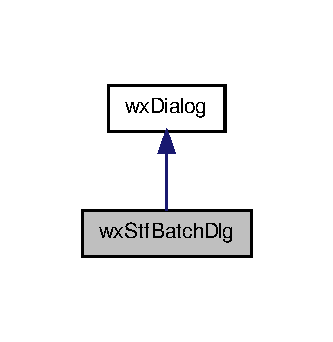
\includegraphics[width=160pt]{classwxStfBatchDlg__inherit__graph}
\end{center}
\end{figure}


Collaboration diagram for wxStfBatchDlg:
\nopagebreak
\begin{figure}[H]
\begin{center}
\leavevmode
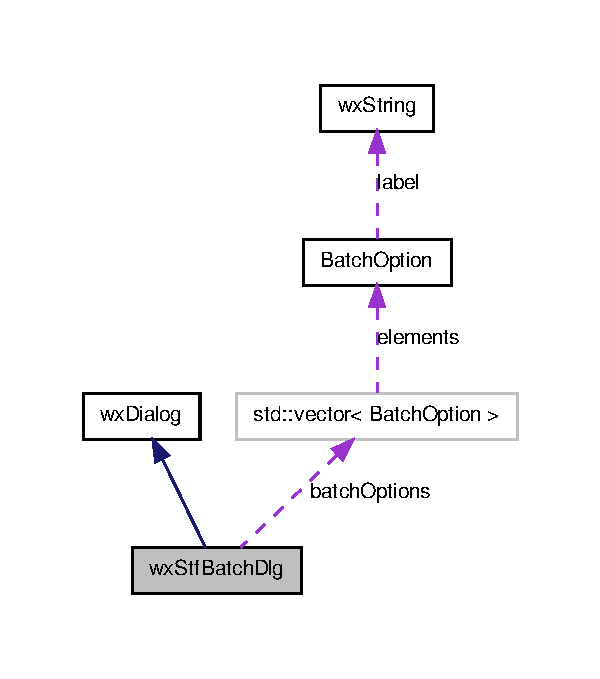
\includegraphics[width=288pt]{classwxStfBatchDlg__coll__graph}
\end{center}
\end{figure}
\subsection*{Public Member Functions}
\begin{DoxyCompactItemize}
\item 
\hyperlink{classwxStfBatchDlg_a675ec9b423de62fdf8b6338ac105ed5a}{wxStfBatchDlg} (\hyperlink{classwxWindow}{wxWindow} $\ast$parent, int id=wxID\_\-ANY, \hyperlink{classwxString}{wxString} title=wxT(\char`\"{}Choose values\char`\"{}), wxPoint pos=wxDefaultPosition, \hyperlink{classwxSize}{wxSize} size=wxDefaultSize, int style=wxCAPTION)
\begin{DoxyCompactList}\small\item\em Constructor. \item\end{DoxyCompactList}\item 
bool \hyperlink{classwxStfBatchDlg_a4cf3b7330fba6d6a39aff6894d534ddc}{PrintBase} () const 
\begin{DoxyCompactList}\small\item\em Indicates whether the baseline should be printed in the batch analysis table. \item\end{DoxyCompactList}\item 
bool \hyperlink{classwxStfBatchDlg_a9f6762e76bbe7657ee3acbf305f81bfc}{PrintBaseSD} () const 
\begin{DoxyCompactList}\small\item\em Indicates whether the standard deviation of the baseline should be printed in the batch analysis table. \item\end{DoxyCompactList}\item 
bool \hyperlink{classwxStfBatchDlg_a79d3b5f5870dafc7a410611cef0605e7}{PrintThreshold} () const 
\begin{DoxyCompactList}\small\item\em Indicates whether the threshold should be printed in the batch analysis table. \item\end{DoxyCompactList}\item 
bool \hyperlink{classwxStfBatchDlg_afa1c7b24cef42c6a97eb4b949282a633}{PrintPeakZero} () const 
\begin{DoxyCompactList}\small\item\em Indicates whether the peak (from 0) value should be printed in the batch analysis table. \item\end{DoxyCompactList}\item 
bool \hyperlink{classwxStfBatchDlg_a8013a833a5c69caf27e7f0075fe76e9f}{PrintPeakBase} () const 
\begin{DoxyCompactList}\small\item\em Indicates whether the peak (from baseline) value should be printed in the batch analysis table. \item\end{DoxyCompactList}\item 
bool \hyperlink{classwxStfBatchDlg_a81f6af94be37c627dfe193fac0fb693f}{PrintPeakThreshold} () const 
\begin{DoxyCompactList}\small\item\em Indicates whether the peak value (from threshold) should be printed in the batch analysis table. \item\end{DoxyCompactList}\item 
bool \hyperlink{classwxStfBatchDlg_a74d582caee2ab99657ab8c4a090009f3}{PrintRT2080} () const 
\begin{DoxyCompactList}\small\item\em Indicates whether the 20-\/80\% rise time should be printed in the batch analysis table. \item\end{DoxyCompactList}\item 
bool \hyperlink{classwxStfBatchDlg_aec7076455bc0744df4b20a09385c0631}{PrintT50} () const 
\begin{DoxyCompactList}\small\item\em Indicates whether the half duration should be printed in the batch analysis table. \item\end{DoxyCompactList}\item 
bool \hyperlink{classwxStfBatchDlg_ae88619770e9b047126c181952cb57b90}{PrintSlopes} () const 
\begin{DoxyCompactList}\small\item\em Indicates whether the maximal slopes should be printed in the batch analysis table. \item\end{DoxyCompactList}\item 
bool \hyperlink{classwxStfBatchDlg_ab4443346bca295b1f4dca3ff1915db90}{PrintThr} () const 
\begin{DoxyCompactList}\small\item\em Indicates whether a threshold crossing should be printed in the batch analysis table. \item\end{DoxyCompactList}\item 
bool \hyperlink{classwxStfBatchDlg_a65df76a1b970ac61623e117563de4fd0}{PrintLatencies} () const 
\begin{DoxyCompactList}\small\item\em Indicates whether the latency should be printed in the batch analysis table. \item\end{DoxyCompactList}\item 
bool \hyperlink{classwxStfBatchDlg_ad4fbdf11777e9e011f9981517f776e3c}{PrintFitResults} () const 
\begin{DoxyCompactList}\small\item\em Indicates whether the fit results should be printed in the batch analysis table. \item\end{DoxyCompactList}\item 
virtual void \hyperlink{classwxStfBatchDlg_a5a2d868fbe377520b8193f7817559173}{EndModal} (int retCode)
\begin{DoxyCompactList}\small\item\em Called upon ending a modal dialog. \item\end{DoxyCompactList}\end{DoxyCompactItemize}


\subsection{Detailed Description}
Dialog for batch analysis settings. 

\subsection{Constructor \& Destructor Documentation}
\hypertarget{classwxStfBatchDlg_a675ec9b423de62fdf8b6338ac105ed5a}{
\index{wxStfBatchDlg@{wxStfBatchDlg}!wxStfBatchDlg@{wxStfBatchDlg}}
\index{wxStfBatchDlg@{wxStfBatchDlg}!wxStfBatchDlg@{wxStfBatchDlg}}
\subsubsection[{wxStfBatchDlg}]{\setlength{\rightskip}{0pt plus 5cm}wxStfBatchDlg::wxStfBatchDlg (
\begin{DoxyParamCaption}
\item[{{\bf wxWindow} $\ast$}]{parent, }
\item[{int}]{id = {\ttfamily wxID\_\-ANY}, }
\item[{{\bf wxString}}]{title = {\ttfamily wxT(\char`\"{}Choose~values\char`\"{})}, }
\item[{{\bf wxPoint}}]{pos = {\ttfamily wxDefaultPosition}, }
\item[{{\bf wxSize}}]{size = {\ttfamily wxDefaultSize}, }
\item[{int}]{style = {\ttfamily wxCAPTION}}
\end{DoxyParamCaption}
)}}
\label{classwxStfBatchDlg_a675ec9b423de62fdf8b6338ac105ed5a}


Constructor. 


\begin{DoxyParams}{Parameters}
{\em parent} & Pointer to parent window. \\
\hline
{\em id} & Window id. \\
\hline
{\em title} & Dialog title. \\
\hline
{\em pos} & Initial position. \\
\hline
{\em size} & Initial size. \\
\hline
{\em style} & Dialog style. \\
\hline
\end{DoxyParams}


\subsection{Member Function Documentation}
\hypertarget{classwxStfBatchDlg_a5a2d868fbe377520b8193f7817559173}{
\index{wxStfBatchDlg@{wxStfBatchDlg}!EndModal@{EndModal}}
\index{EndModal@{EndModal}!wxStfBatchDlg@{wxStfBatchDlg}}
\subsubsection[{EndModal}]{\setlength{\rightskip}{0pt plus 5cm}virtual void wxStfBatchDlg::EndModal (
\begin{DoxyParamCaption}
\item[{int}]{retCode}
\end{DoxyParamCaption}
)\hspace{0.3cm}{\ttfamily  \mbox{[}virtual\mbox{]}}}}
\label{classwxStfBatchDlg_a5a2d868fbe377520b8193f7817559173}


Called upon ending a modal dialog. 


\begin{DoxyParams}{Parameters}
{\em retCode} & The dialog button id that ended the dialog (e.g. wxID\_\-OK) \\
\hline
\end{DoxyParams}
\hypertarget{classwxStfBatchDlg_a4cf3b7330fba6d6a39aff6894d534ddc}{
\index{wxStfBatchDlg@{wxStfBatchDlg}!PrintBase@{PrintBase}}
\index{PrintBase@{PrintBase}!wxStfBatchDlg@{wxStfBatchDlg}}
\subsubsection[{PrintBase}]{\setlength{\rightskip}{0pt plus 5cm}bool wxStfBatchDlg::PrintBase (
\begin{DoxyParamCaption}
{}
\end{DoxyParamCaption}
) const\hspace{0.3cm}{\ttfamily  \mbox{[}inline\mbox{]}}}}
\label{classwxStfBatchDlg_a4cf3b7330fba6d6a39aff6894d534ddc}


Indicates whether the baseline should be printed in the batch analysis table. 

\begin{DoxyReturn}{Returns}
true if it should be printed, false otherwise. 
\end{DoxyReturn}


References BatchOption::selection.

\hypertarget{classwxStfBatchDlg_a9f6762e76bbe7657ee3acbf305f81bfc}{
\index{wxStfBatchDlg@{wxStfBatchDlg}!PrintBaseSD@{PrintBaseSD}}
\index{PrintBaseSD@{PrintBaseSD}!wxStfBatchDlg@{wxStfBatchDlg}}
\subsubsection[{PrintBaseSD}]{\setlength{\rightskip}{0pt plus 5cm}bool wxStfBatchDlg::PrintBaseSD (
\begin{DoxyParamCaption}
{}
\end{DoxyParamCaption}
) const\hspace{0.3cm}{\ttfamily  \mbox{[}inline\mbox{]}}}}
\label{classwxStfBatchDlg_a9f6762e76bbe7657ee3acbf305f81bfc}


Indicates whether the standard deviation of the baseline should be printed in the batch analysis table. 

\begin{DoxyReturn}{Returns}
true if it should be printed, false otherwise. 
\end{DoxyReturn}


References BatchOption::selection.

\hypertarget{classwxStfBatchDlg_ad4fbdf11777e9e011f9981517f776e3c}{
\index{wxStfBatchDlg@{wxStfBatchDlg}!PrintFitResults@{PrintFitResults}}
\index{PrintFitResults@{PrintFitResults}!wxStfBatchDlg@{wxStfBatchDlg}}
\subsubsection[{PrintFitResults}]{\setlength{\rightskip}{0pt plus 5cm}bool wxStfBatchDlg::PrintFitResults (
\begin{DoxyParamCaption}
{}
\end{DoxyParamCaption}
) const\hspace{0.3cm}{\ttfamily  \mbox{[}inline\mbox{]}}}}
\label{classwxStfBatchDlg_ad4fbdf11777e9e011f9981517f776e3c}


Indicates whether the fit results should be printed in the batch analysis table. 

\begin{DoxyReturn}{Returns}
true if it should be printed, false otherwise. 
\end{DoxyReturn}


References BatchOption::selection.

\hypertarget{classwxStfBatchDlg_a65df76a1b970ac61623e117563de4fd0}{
\index{wxStfBatchDlg@{wxStfBatchDlg}!PrintLatencies@{PrintLatencies}}
\index{PrintLatencies@{PrintLatencies}!wxStfBatchDlg@{wxStfBatchDlg}}
\subsubsection[{PrintLatencies}]{\setlength{\rightskip}{0pt plus 5cm}bool wxStfBatchDlg::PrintLatencies (
\begin{DoxyParamCaption}
{}
\end{DoxyParamCaption}
) const\hspace{0.3cm}{\ttfamily  \mbox{[}inline\mbox{]}}}}
\label{classwxStfBatchDlg_a65df76a1b970ac61623e117563de4fd0}


Indicates whether the latency should be printed in the batch analysis table. 

\begin{DoxyReturn}{Returns}
true if it should be printed, false otherwise. 
\end{DoxyReturn}


References BatchOption::selection.

\hypertarget{classwxStfBatchDlg_a8013a833a5c69caf27e7f0075fe76e9f}{
\index{wxStfBatchDlg@{wxStfBatchDlg}!PrintPeakBase@{PrintPeakBase}}
\index{PrintPeakBase@{PrintPeakBase}!wxStfBatchDlg@{wxStfBatchDlg}}
\subsubsection[{PrintPeakBase}]{\setlength{\rightskip}{0pt plus 5cm}bool wxStfBatchDlg::PrintPeakBase (
\begin{DoxyParamCaption}
{}
\end{DoxyParamCaption}
) const\hspace{0.3cm}{\ttfamily  \mbox{[}inline\mbox{]}}}}
\label{classwxStfBatchDlg_a8013a833a5c69caf27e7f0075fe76e9f}


Indicates whether the peak (from baseline) value should be printed in the batch analysis table. 

\begin{DoxyReturn}{Returns}
true if it should be printed, false otherwise. 
\end{DoxyReturn}


References BatchOption::selection.

\hypertarget{classwxStfBatchDlg_a81f6af94be37c627dfe193fac0fb693f}{
\index{wxStfBatchDlg@{wxStfBatchDlg}!PrintPeakThreshold@{PrintPeakThreshold}}
\index{PrintPeakThreshold@{PrintPeakThreshold}!wxStfBatchDlg@{wxStfBatchDlg}}
\subsubsection[{PrintPeakThreshold}]{\setlength{\rightskip}{0pt plus 5cm}bool wxStfBatchDlg::PrintPeakThreshold (
\begin{DoxyParamCaption}
{}
\end{DoxyParamCaption}
) const\hspace{0.3cm}{\ttfamily  \mbox{[}inline\mbox{]}}}}
\label{classwxStfBatchDlg_a81f6af94be37c627dfe193fac0fb693f}


Indicates whether the peak value (from threshold) should be printed in the batch analysis table. 

\begin{DoxyReturn}{Returns}
true if it should be printed, false otherwise. 
\end{DoxyReturn}


References BatchOption::selection.

\hypertarget{classwxStfBatchDlg_afa1c7b24cef42c6a97eb4b949282a633}{
\index{wxStfBatchDlg@{wxStfBatchDlg}!PrintPeakZero@{PrintPeakZero}}
\index{PrintPeakZero@{PrintPeakZero}!wxStfBatchDlg@{wxStfBatchDlg}}
\subsubsection[{PrintPeakZero}]{\setlength{\rightskip}{0pt plus 5cm}bool wxStfBatchDlg::PrintPeakZero (
\begin{DoxyParamCaption}
{}
\end{DoxyParamCaption}
) const\hspace{0.3cm}{\ttfamily  \mbox{[}inline\mbox{]}}}}
\label{classwxStfBatchDlg_afa1c7b24cef42c6a97eb4b949282a633}


Indicates whether the peak (from 0) value should be printed in the batch analysis table. 

\begin{DoxyReturn}{Returns}
true if it should be printed, false otherwise. 
\end{DoxyReturn}


References BatchOption::selection.

\hypertarget{classwxStfBatchDlg_a74d582caee2ab99657ab8c4a090009f3}{
\index{wxStfBatchDlg@{wxStfBatchDlg}!PrintRT2080@{PrintRT2080}}
\index{PrintRT2080@{PrintRT2080}!wxStfBatchDlg@{wxStfBatchDlg}}
\subsubsection[{PrintRT2080}]{\setlength{\rightskip}{0pt plus 5cm}bool wxStfBatchDlg::PrintRT2080 (
\begin{DoxyParamCaption}
{}
\end{DoxyParamCaption}
) const\hspace{0.3cm}{\ttfamily  \mbox{[}inline\mbox{]}}}}
\label{classwxStfBatchDlg_a74d582caee2ab99657ab8c4a090009f3}


Indicates whether the 20-\/80\% rise time should be printed in the batch analysis table. 

\begin{DoxyReturn}{Returns}
true if it should be printed, false otherwise. 
\end{DoxyReturn}


References BatchOption::selection.

\hypertarget{classwxStfBatchDlg_ae88619770e9b047126c181952cb57b90}{
\index{wxStfBatchDlg@{wxStfBatchDlg}!PrintSlopes@{PrintSlopes}}
\index{PrintSlopes@{PrintSlopes}!wxStfBatchDlg@{wxStfBatchDlg}}
\subsubsection[{PrintSlopes}]{\setlength{\rightskip}{0pt plus 5cm}bool wxStfBatchDlg::PrintSlopes (
\begin{DoxyParamCaption}
{}
\end{DoxyParamCaption}
) const\hspace{0.3cm}{\ttfamily  \mbox{[}inline\mbox{]}}}}
\label{classwxStfBatchDlg_ae88619770e9b047126c181952cb57b90}


Indicates whether the maximal slopes should be printed in the batch analysis table. 

\begin{DoxyReturn}{Returns}
true if it should be printed, false otherwise. 
\end{DoxyReturn}


References BatchOption::selection.

\hypertarget{classwxStfBatchDlg_aec7076455bc0744df4b20a09385c0631}{
\index{wxStfBatchDlg@{wxStfBatchDlg}!PrintT50@{PrintT50}}
\index{PrintT50@{PrintT50}!wxStfBatchDlg@{wxStfBatchDlg}}
\subsubsection[{PrintT50}]{\setlength{\rightskip}{0pt plus 5cm}bool wxStfBatchDlg::PrintT50 (
\begin{DoxyParamCaption}
{}
\end{DoxyParamCaption}
) const\hspace{0.3cm}{\ttfamily  \mbox{[}inline\mbox{]}}}}
\label{classwxStfBatchDlg_aec7076455bc0744df4b20a09385c0631}


Indicates whether the half duration should be printed in the batch analysis table. 

\begin{DoxyReturn}{Returns}
true if it should be printed, false otherwise. 
\end{DoxyReturn}


References BatchOption::selection.

\hypertarget{classwxStfBatchDlg_ab4443346bca295b1f4dca3ff1915db90}{
\index{wxStfBatchDlg@{wxStfBatchDlg}!PrintThr@{PrintThr}}
\index{PrintThr@{PrintThr}!wxStfBatchDlg@{wxStfBatchDlg}}
\subsubsection[{PrintThr}]{\setlength{\rightskip}{0pt plus 5cm}bool wxStfBatchDlg::PrintThr (
\begin{DoxyParamCaption}
{}
\end{DoxyParamCaption}
) const\hspace{0.3cm}{\ttfamily  \mbox{[}inline\mbox{]}}}}
\label{classwxStfBatchDlg_ab4443346bca295b1f4dca3ff1915db90}


Indicates whether a threshold crossing should be printed in the batch analysis table. 

\begin{DoxyReturn}{Returns}
true if it should be printed, false otherwise. 
\end{DoxyReturn}


References BatchOption::selection.

\hypertarget{classwxStfBatchDlg_a79d3b5f5870dafc7a410611cef0605e7}{
\index{wxStfBatchDlg@{wxStfBatchDlg}!PrintThreshold@{PrintThreshold}}
\index{PrintThreshold@{PrintThreshold}!wxStfBatchDlg@{wxStfBatchDlg}}
\subsubsection[{PrintThreshold}]{\setlength{\rightskip}{0pt plus 5cm}bool wxStfBatchDlg::PrintThreshold (
\begin{DoxyParamCaption}
{}
\end{DoxyParamCaption}
) const\hspace{0.3cm}{\ttfamily  \mbox{[}inline\mbox{]}}}}
\label{classwxStfBatchDlg_a79d3b5f5870dafc7a410611cef0605e7}


Indicates whether the threshold should be printed in the batch analysis table. 

\begin{DoxyReturn}{Returns}
true if it should be printed, false otherwise. 
\end{DoxyReturn}


References BatchOption::selection.



The documentation for this class was generated from the following file:\begin{DoxyCompactItemize}
\item 
src/app/dlgs/\hyperlink{smalldlgs_8h}{smalldlgs.h}\end{DoxyCompactItemize}

\hypertarget{classwxStfChannelSelDlg}{
\section{wxStfChannelSelDlg Class Reference}
\label{classwxStfChannelSelDlg}\index{wxStfChannelSelDlg@{wxStfChannelSelDlg}}
}


Dialog for selecting channels.  




{\ttfamily \#include $<$smalldlgs.h$>$}



Inheritance diagram for wxStfChannelSelDlg:
\nopagebreak
\begin{figure}[H]
\begin{center}
\leavevmode
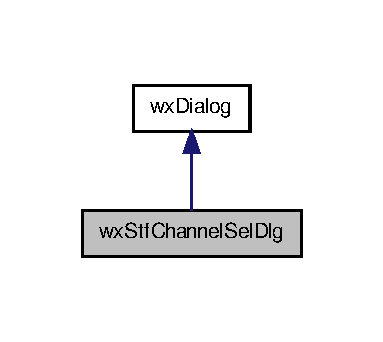
\includegraphics[width=184pt]{classwxStfChannelSelDlg__inherit__graph}
\end{center}
\end{figure}


Collaboration diagram for wxStfChannelSelDlg:
\nopagebreak
\begin{figure}[H]
\begin{center}
\leavevmode
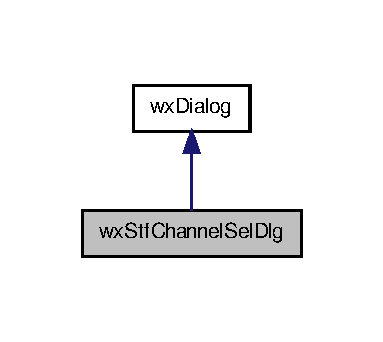
\includegraphics[width=184pt]{classwxStfChannelSelDlg__coll__graph}
\end{center}
\end{figure}
\subsection*{Public Member Functions}
\begin{DoxyCompactItemize}
\item 
\hyperlink{classwxStfChannelSelDlg_ab3a13cce72ce68940804f2cad0a08322}{wxStfChannelSelDlg} (\hyperlink{classwxWindow}{wxWindow} $\ast$parent, const std::vector$<$ \hyperlink{classwxString}{wxString} $>$ \&channelNames=std::vector$<$ \hyperlink{classwxString}{wxString} $>$(0), int id=wxID\_\-ANY, \hyperlink{classwxString}{wxString} title=wxT(\char`\"{}Select channels\char`\"{}), wxPoint pos=wxDefaultPosition, \hyperlink{classwxSize}{wxSize} size=wxDefaultSize, int style=wxCAPTION)
\begin{DoxyCompactList}\small\item\em Constructor. \item\end{DoxyCompactList}\item 
virtual void \hyperlink{classwxStfChannelSelDlg_acd4e03d717bf7f53b248dee9efbf67b5}{EndModal} (int retCode)
\begin{DoxyCompactList}\small\item\em Called upon ending a modal dialog. \item\end{DoxyCompactList}\item 
int \hyperlink{classwxStfChannelSelDlg_a4411792835ba28251e7f25f217a37ec1}{GetSelCh1} () const 
\begin{DoxyCompactList}\small\item\em Get selection for channel 1. \item\end{DoxyCompactList}\item 
int \hyperlink{classwxStfChannelSelDlg_a55f484d5a236a7da3d40f266ec805952}{GetSelCh2} () const 
\begin{DoxyCompactList}\small\item\em Get selection for channel 2. \item\end{DoxyCompactList}\end{DoxyCompactItemize}


\subsection{Detailed Description}
Dialog for selecting channels. 

\subsection{Constructor \& Destructor Documentation}
\hypertarget{classwxStfChannelSelDlg_ab3a13cce72ce68940804f2cad0a08322}{
\index{wxStfChannelSelDlg@{wxStfChannelSelDlg}!wxStfChannelSelDlg@{wxStfChannelSelDlg}}
\index{wxStfChannelSelDlg@{wxStfChannelSelDlg}!wxStfChannelSelDlg@{wxStfChannelSelDlg}}
\subsubsection[{wxStfChannelSelDlg}]{\setlength{\rightskip}{0pt plus 5cm}wxStfChannelSelDlg::wxStfChannelSelDlg (
\begin{DoxyParamCaption}
\item[{{\bf wxWindow} $\ast$}]{parent, }
\item[{const std::vector$<$ {\bf wxString} $>$ \&}]{channelNames = {\ttfamily std::vector$<$~{\bf wxString}~$>$(0)}, }
\item[{int}]{id = {\ttfamily wxID\_\-ANY}, }
\item[{{\bf wxString}}]{title = {\ttfamily wxT(\char`\"{}Select~channels\char`\"{})}, }
\item[{{\bf wxPoint}}]{pos = {\ttfamily wxDefaultPosition}, }
\item[{{\bf wxSize}}]{size = {\ttfamily wxDefaultSize}, }
\item[{int}]{style = {\ttfamily wxCAPTION}}
\end{DoxyParamCaption}
)}}
\label{classwxStfChannelSelDlg_ab3a13cce72ce68940804f2cad0a08322}


Constructor. 


\begin{DoxyParams}{Parameters}
{\em parent} & Pointer to parent window. \\
\hline
{\em channelNames} & A vector containing the channel names. \\
\hline
{\em id} & Window id. \\
\hline
{\em title} & Dialog title. \\
\hline
{\em pos} & Initial position. \\
\hline
{\em size} & Initial size. \\
\hline
{\em style} & Dialog style. \\
\hline
\end{DoxyParams}


\subsection{Member Function Documentation}
\hypertarget{classwxStfChannelSelDlg_acd4e03d717bf7f53b248dee9efbf67b5}{
\index{wxStfChannelSelDlg@{wxStfChannelSelDlg}!EndModal@{EndModal}}
\index{EndModal@{EndModal}!wxStfChannelSelDlg@{wxStfChannelSelDlg}}
\subsubsection[{EndModal}]{\setlength{\rightskip}{0pt plus 5cm}virtual void wxStfChannelSelDlg::EndModal (
\begin{DoxyParamCaption}
\item[{int}]{retCode}
\end{DoxyParamCaption}
)\hspace{0.3cm}{\ttfamily  \mbox{[}virtual\mbox{]}}}}
\label{classwxStfChannelSelDlg_acd4e03d717bf7f53b248dee9efbf67b5}


Called upon ending a modal dialog. 


\begin{DoxyParams}{Parameters}
{\em retCode} & The dialog button id that ended the dialog (e.g. wxID\_\-OK) \\
\hline
\end{DoxyParams}
\hypertarget{classwxStfChannelSelDlg_a4411792835ba28251e7f25f217a37ec1}{
\index{wxStfChannelSelDlg@{wxStfChannelSelDlg}!GetSelCh1@{GetSelCh1}}
\index{GetSelCh1@{GetSelCh1}!wxStfChannelSelDlg@{wxStfChannelSelDlg}}
\subsubsection[{GetSelCh1}]{\setlength{\rightskip}{0pt plus 5cm}int wxStfChannelSelDlg::GetSelCh1 (
\begin{DoxyParamCaption}
{}
\end{DoxyParamCaption}
) const\hspace{0.3cm}{\ttfamily  \mbox{[}inline\mbox{]}}}}
\label{classwxStfChannelSelDlg_a4411792835ba28251e7f25f217a37ec1}


Get selection for channel 1. 

\begin{DoxyReturn}{Returns}
The index of the first (active) channel 
\end{DoxyReturn}
\hypertarget{classwxStfChannelSelDlg_a55f484d5a236a7da3d40f266ec805952}{
\index{wxStfChannelSelDlg@{wxStfChannelSelDlg}!GetSelCh2@{GetSelCh2}}
\index{GetSelCh2@{GetSelCh2}!wxStfChannelSelDlg@{wxStfChannelSelDlg}}
\subsubsection[{GetSelCh2}]{\setlength{\rightskip}{0pt plus 5cm}int wxStfChannelSelDlg::GetSelCh2 (
\begin{DoxyParamCaption}
{}
\end{DoxyParamCaption}
) const\hspace{0.3cm}{\ttfamily  \mbox{[}inline\mbox{]}}}}
\label{classwxStfChannelSelDlg_a55f484d5a236a7da3d40f266ec805952}


Get selection for channel 2. 

\begin{DoxyReturn}{Returns}
The index of the second (inactive) channel 
\end{DoxyReturn}


The documentation for this class was generated from the following file:\begin{DoxyCompactItemize}
\item 
src/app/dlgs/\hyperlink{smalldlgs_8h}{smalldlgs.h}\end{DoxyCompactItemize}

\hypertarget{classwxStfCheckBox}{
\section{wxStfCheckBox Class Reference}
\label{classwxStfCheckBox}\index{wxStfCheckBox@{wxStfCheckBox}}
}


A checkbox used to select or unselect detected events.  




{\ttfamily \#include $<$stfcheckbox.h$>$}



Inheritance diagram for wxStfCheckBox:
\nopagebreak
\begin{figure}[H]
\begin{center}
\leavevmode
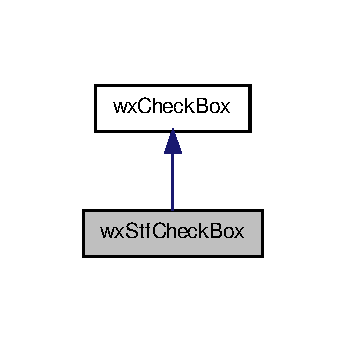
\includegraphics[width=166pt]{classwxStfCheckBox__inherit__graph}
\end{center}
\end{figure}


Collaboration diagram for wxStfCheckBox:
\nopagebreak
\begin{figure}[H]
\begin{center}
\leavevmode
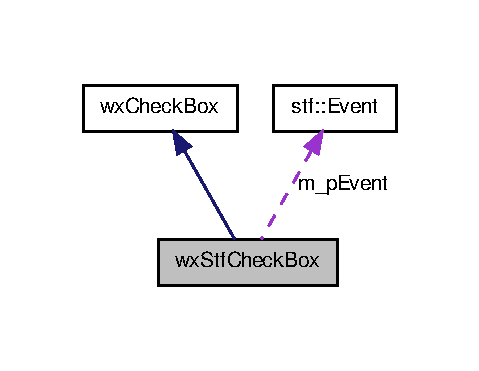
\includegraphics[width=230pt]{classwxStfCheckBox__coll__graph}
\end{center}
\end{figure}
\subsection*{Public Member Functions}
\begin{DoxyCompactItemize}
\item 
\hyperlink{classwxStfCheckBox_a9c976112e0951a799ff63f6c491a159b}{wxStfCheckBox} (\hyperlink{classwxWindow}{wxWindow} $\ast$parent, wxWindowID id, const \hyperlink{classwxString}{wxString} \&label, \hyperlink{classstf_1_1Event}{stf::Event} $\ast$pEvent, const \hyperlink{classwxPoint}{wxPoint} \&pos=wxDefaultPosition, const \hyperlink{classwxSize}{wxSize} \&size=wxDefaultSize, long style=0, const wxValidator \&validator=wxDefaultValidator, const \hyperlink{classwxString}{wxString} \&name=wxCheckBoxNameStr)
\begin{DoxyCompactList}\small\item\em Constructor. \item\end{DoxyCompactList}\item 
void \hyperlink{classwxStfCheckBox_a29d01f441967d73be7fa05e9d722fd5d}{ResetEvent} (\hyperlink{classstf_1_1Event}{stf::Event} $\ast$pEvent)
\begin{DoxyCompactList}\small\item\em Resets the pointer to the attached event. \item\end{DoxyCompactList}\end{DoxyCompactItemize}


\subsection{Detailed Description}
A checkbox used to select or unselect detected events. Toggles the \hyperlink{classstf_1_1Event}{stf::Event} status, and forwards keyboard input to the graph. 

\subsection{Constructor \& Destructor Documentation}
\hypertarget{classwxStfCheckBox_a9c976112e0951a799ff63f6c491a159b}{
\index{wxStfCheckBox@{wxStfCheckBox}!wxStfCheckBox@{wxStfCheckBox}}
\index{wxStfCheckBox@{wxStfCheckBox}!wxStfCheckBox@{wxStfCheckBox}}
\subsubsection[{wxStfCheckBox}]{\setlength{\rightskip}{0pt plus 5cm}wxStfCheckBox::wxStfCheckBox (
\begin{DoxyParamCaption}
\item[{{\bf wxWindow} $\ast$}]{parent, }
\item[{wxWindowID}]{id, }
\item[{const {\bf wxString} \&}]{label, }
\item[{{\bf stf::Event} $\ast$}]{pEvent, }
\item[{const {\bf wxPoint} \&}]{pos = {\ttfamily wxDefaultPosition}, }
\item[{const {\bf wxSize} \&}]{size = {\ttfamily wxDefaultSize}, }
\item[{long}]{style = {\ttfamily 0}, }
\item[{const wxValidator \&}]{validator = {\ttfamily wxDefaultValidator}, }
\item[{const {\bf wxString} \&}]{name = {\ttfamily wxCheckBoxNameStr}}
\end{DoxyParamCaption}
)}}
\label{classwxStfCheckBox_a9c976112e0951a799ff63f6c491a159b}


Constructor. 


\begin{DoxyParams}{Parameters}
{\em parent} & Pointer to the parent window. \\
\hline
{\em id} & Window id. \\
\hline
{\em label} & The checkbox label. \\
\hline
{\em pEvent} & The event attached to this checkbox. \\
\hline
{\em pos} & Initial checkbox position. \\
\hline
{\em size} & Initial checkbox size. \\
\hline
{\em style} & Checkbox style. \\
\hline
{\em validator} & Checkbox validator. \\
\hline
{\em name} & Name of this grid. \\
\hline
\end{DoxyParams}


\subsection{Member Function Documentation}
\hypertarget{classwxStfCheckBox_a29d01f441967d73be7fa05e9d722fd5d}{
\index{wxStfCheckBox@{wxStfCheckBox}!ResetEvent@{ResetEvent}}
\index{ResetEvent@{ResetEvent}!wxStfCheckBox@{wxStfCheckBox}}
\subsubsection[{ResetEvent}]{\setlength{\rightskip}{0pt plus 5cm}void wxStfCheckBox::ResetEvent (
\begin{DoxyParamCaption}
\item[{{\bf stf::Event} $\ast$}]{pEvent}
\end{DoxyParamCaption}
)\hspace{0.3cm}{\ttfamily  \mbox{[}inline\mbox{]}}}}
\label{classwxStfCheckBox_a29d01f441967d73be7fa05e9d722fd5d}


Resets the pointer to the attached event. 


\begin{DoxyParams}{Parameters}
{\em pEvent} & The pointer to the new event \\
\hline
\end{DoxyParams}


References stf::Event::GetDiscard().



The documentation for this class was generated from the following file:\begin{DoxyCompactItemize}
\item 
src/app/\hyperlink{stfcheckbox_8h}{stfcheckbox.h}\end{DoxyCompactItemize}

\hypertarget{classwxStfChildFrame}{
\section{wxStfChildFrame Class Reference}
\label{classwxStfChildFrame}\index{wxStfChildFrame@{wxStfChildFrame}}
}


Provides the child frame for displaying documents on separate windows.  




{\ttfamily \#include $<$childframe.h$>$}



Inheritance diagram for wxStfChildFrame:
\nopagebreak
\begin{figure}[H]
\begin{center}
\leavevmode
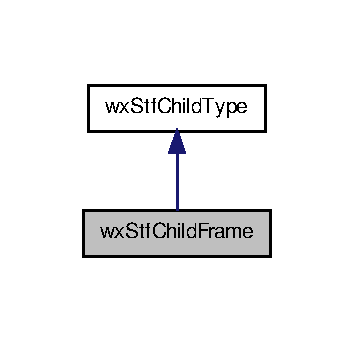
\includegraphics[width=170pt]{classwxStfChildFrame__inherit__graph}
\end{center}
\end{figure}


Collaboration diagram for wxStfChildFrame:
\nopagebreak
\begin{figure}[H]
\begin{center}
\leavevmode
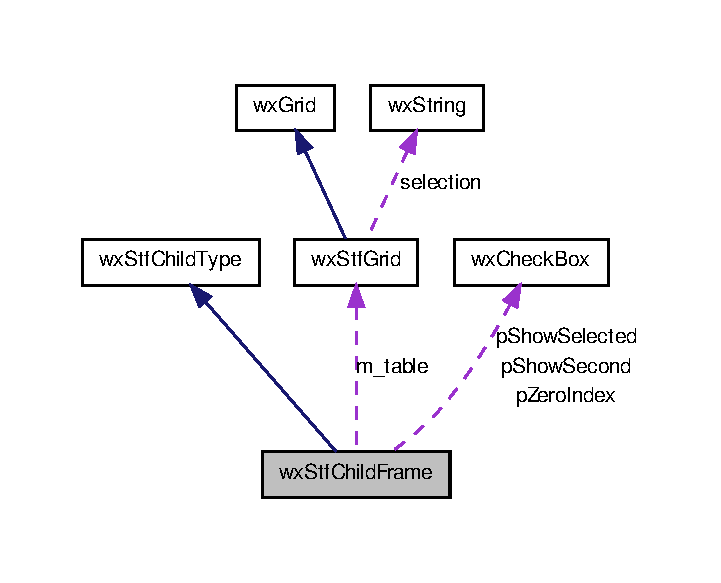
\includegraphics[width=346pt]{classwxStfChildFrame__coll__graph}
\end{center}
\end{figure}
\subsection*{Public Member Functions}
\begin{DoxyCompactItemize}
\item 
\hyperlink{classwxStfChildFrame_ad0da3136456c372aac1a26264a05cf88}{wxStfChildFrame} (\hyperlink{classwxDocument}{wxDocument} $\ast$doc, \hyperlink{classwxView}{wxView} $\ast$view, \hyperlink{classwxDocMDIParentFrame}{wxStfParentType} $\ast$parent, wxWindowID id, const \hyperlink{classwxString}{wxString} \&title, const \hyperlink{classwxPoint}{wxPoint} \&pos=\hyperlink{classwxPoint}{wxPoint}(48, 48), const \hyperlink{classwxSize}{wxSize} \&size=wxDefaultSize, long style=wxDEFAULT\_\-FRAME\_\-STYLE, const \hyperlink{classwxString}{wxString} \&name=wxT(\char`\"{}frame\char`\"{}))
\begin{DoxyCompactList}\small\item\em Constructor. \item\end{DoxyCompactList}\item 
\hypertarget{classwxStfChildFrame_ab4d598cb9650ba0734aa9c9a82b1e6a6}{
\hyperlink{classwxStfChildFrame_ab4d598cb9650ba0734aa9c9a82b1e6a6}{$\sim$wxStfChildFrame} ()}
\label{classwxStfChildFrame_ab4d598cb9650ba0734aa9c9a82b1e6a6}

\begin{DoxyCompactList}\small\item\em Destructor. \item\end{DoxyCompactList}\item 
void \hyperlink{classwxStfChildFrame_a5eed0f028a05cfd1d967baddd926808e}{ShowTable} (const \hyperlink{classstf_1_1Table}{stf::Table} \&table, const \hyperlink{classwxString}{wxString} \&caption)
\begin{DoxyCompactList}\small\item\em Adds a table to the results notebook. \item\end{DoxyCompactList}\item 
std::size\_\-t \hyperlink{classwxStfChildFrame_a5d3d4ccb9139d9b89a1d8c3b5274bf44}{GetCurTrace} () const 
\begin{DoxyCompactList}\small\item\em Retrieves the current trace from the trace selection combo box. \item\end{DoxyCompactList}\item 
void \hyperlink{classwxStfChildFrame_ac4951640416b40c7ef770972b2861a96}{SetCurTrace} (std::size\_\-t)
\begin{DoxyCompactList}\small\item\em Sets the current trace from the trace selection combo box. \item\end{DoxyCompactList}\item 
void \hyperlink{classwxStfChildFrame_a8bf15457066b27f81c4ce7f6efee0968}{CreateMenuTraces} (std::size\_\-t value)
\begin{DoxyCompactList}\small\item\em Creates the trace selection menu. \item\end{DoxyCompactList}\item 
void \hyperlink{classwxStfChildFrame_ad2ae8f658f6cf4e5ab293fce15c2ef72}{CreateComboChannels} (const wxArrayString \&channelNames)
\begin{DoxyCompactList}\small\item\em Creates the channel selection combo boxes. \item\end{DoxyCompactList}\item 
void \hyperlink{classwxStfChildFrame_a1378a98bc5cbb3983398cbaa4df07b14}{SetSelected} (std::size\_\-t value)
\begin{DoxyCompactList}\small\item\em Refreshes the trace selection string. \item\end{DoxyCompactList}\item 
void \hyperlink{classwxStfChildFrame_a4dcae3a72bd8cbf4ec88fa8c175a5263}{SetChannels} (std::size\_\-t act, std::size\_\-t inact)
\begin{DoxyCompactList}\small\item\em Sets the channels in the combo boxes. Checks and corrects equal channels in both boxes. \item\end{DoxyCompactList}\item 
\hypertarget{classwxStfChildFrame_ad51c5aaa777d50ce3577bacc5c282ca4}{
void \hyperlink{classwxStfChildFrame_ad51c5aaa777d50ce3577bacc5c282ca4}{UpdateChannels} ()}
\label{classwxStfChildFrame_ad51c5aaa777d50ce3577bacc5c282ca4}

\begin{DoxyCompactList}\small\item\em Updates the channels according to the current combo boy selection. \item\end{DoxyCompactList}\item 
void \hyperlink{classwxStfChildFrame_aa74cf4d2706de49d7e62c6ce7bffa2e6}{UpdateResults} ()
\begin{DoxyCompactList}\small\item\em Updates the results table. \item\end{DoxyCompactList}\item 
wxAuiManager $\ast$ \hyperlink{classwxStfChildFrame_a68df0de27a7818fc273e23e3773fd0da}{GetMgr} ()
\begin{DoxyCompactList}\small\item\em Retrieve the wxAuiManager. \item\end{DoxyCompactList}\item 
\hyperlink{classwxStfGrid}{wxStfGrid} $\ast$ \hyperlink{classwxStfChildFrame_a4e2fab6fd5eea1a8da903bac45823fef}{GetCopyGrid} ()
\begin{DoxyCompactList}\small\item\em Retrieve the \hyperlink{classwxStfGrid}{wxStfGrid} that contains the results table. \item\end{DoxyCompactList}\item 
\hypertarget{classwxStfChildFrame_ab3d88fc327c7f4dcfde46f4764a02152}{
void \hyperlink{classwxStfChildFrame_ab3d88fc327c7f4dcfde46f4764a02152}{Saveperspective} ()}
\label{classwxStfChildFrame_ab3d88fc327c7f4dcfde46f4764a02152}

\begin{DoxyCompactList}\small\item\em Write the current AUI perspective to the configuration. \item\end{DoxyCompactList}\item 
\hypertarget{classwxStfChildFrame_a5e3b3b5ed6f0e91542051a7320ee3fb5}{
void \hyperlink{classwxStfChildFrame_a5e3b3b5ed6f0e91542051a7320ee3fb5}{Loadperspective} ()}
\label{classwxStfChildFrame_a5e3b3b5ed6f0e91542051a7320ee3fb5}

\begin{DoxyCompactList}\small\item\em Load the saved AUI perspective from the configuration. \item\end{DoxyCompactList}\item 
\hypertarget{classwxStfChildFrame_a9ca8d5334433e39f014a399b26589d32}{
void \hyperlink{classwxStfChildFrame_a9ca8d5334433e39f014a399b26589d32}{Restoreperspective} ()}
\label{classwxStfChildFrame_a9ca8d5334433e39f014a399b26589d32}

\begin{DoxyCompactList}\small\item\em Restore the default AUI perspective. \item\end{DoxyCompactList}\item 
bool \hyperlink{classwxStfChildFrame_a6d956a35f7e01c0bf18ca1409b5f50e0}{ShowSelected} () const 
\begin{DoxyCompactList}\small\item\em Indicates whether all selected traces should be plotted. \item\end{DoxyCompactList}\item 
bool \hyperlink{classwxStfChildFrame_aeab6592a78f2b567c46b716dbbdcac70}{ShowSecond} () const 
\begin{DoxyCompactList}\small\item\em Indicates whether the second channel should be plotted. \item\end{DoxyCompactList}\item 
\hypertarget{classwxStfChildFrame_a0186c699805f1f99befae295f864bcbe}{
void \hyperlink{classwxStfChildFrame_a0186c699805f1f99befae295f864bcbe}{ActivateGraph} ()}
\label{classwxStfChildFrame_a0186c699805f1f99befae295f864bcbe}

\begin{DoxyCompactList}\small\item\em Activated the current graph. \item\end{DoxyCompactList}\item 
\hypertarget{classwxStfChildFrame_ac12d539c58c7826a616b259d345859e6}{
void {\bfseries OnActivate} (wxActivateEvent \&event)}
\label{classwxStfChildFrame_ac12d539c58c7826a616b259d345859e6}

\end{DoxyCompactItemize}


\subsection{Detailed Description}
Provides the child frame for displaying documents on separate windows. This class can only be used for MDI child frames. It is part of the document/view framework supported by wxWidgets. 

\subsection{Constructor \& Destructor Documentation}
\hypertarget{classwxStfChildFrame_ad0da3136456c372aac1a26264a05cf88}{
\index{wxStfChildFrame@{wxStfChildFrame}!wxStfChildFrame@{wxStfChildFrame}}
\index{wxStfChildFrame@{wxStfChildFrame}!wxStfChildFrame@{wxStfChildFrame}}
\subsubsection[{wxStfChildFrame}]{\setlength{\rightskip}{0pt plus 5cm}wxStfChildFrame::wxStfChildFrame (
\begin{DoxyParamCaption}
\item[{{\bf wxDocument} $\ast$}]{doc, }
\item[{{\bf wxView} $\ast$}]{view, }
\item[{{\bf wxStfParentType} $\ast$}]{parent, }
\item[{wxWindowID}]{id, }
\item[{const {\bf wxString} \&}]{title, }
\item[{const {\bf wxPoint} \&}]{pos = {\ttfamily {\bf wxPoint}(48,~48)}, }
\item[{const {\bf wxSize} \&}]{size = {\ttfamily wxDefaultSize}, }
\item[{long}]{style = {\ttfamily wxDEFAULT\_\-FRAME\_\-STYLE}, }
\item[{const {\bf wxString} \&}]{name = {\ttfamily wxT(\char`\"{}frame\char`\"{})}}
\end{DoxyParamCaption}
)}}
\label{classwxStfChildFrame_ad0da3136456c372aac1a26264a05cf88}


Constructor. 


\begin{DoxyParams}{Parameters}
{\em doc} & Pointer to the attached document. \\
\hline
{\em view} & Pointer to the attached view. \\
\hline
{\em parent} & Pointer to the parent frame. \\
\hline
{\em id} & Window id. \\
\hline
{\em title} & Window title string. \\
\hline
{\em pos} & Initial window position. \\
\hline
{\em size} & Initial window size. \\
\hline
{\em style} & Window style. \\
\hline
{\em name} & Name of this frame. \\
\hline
\end{DoxyParams}


\subsection{Member Function Documentation}
\hypertarget{classwxStfChildFrame_ad2ae8f658f6cf4e5ab293fce15c2ef72}{
\index{wxStfChildFrame@{wxStfChildFrame}!CreateComboChannels@{CreateComboChannels}}
\index{CreateComboChannels@{CreateComboChannels}!wxStfChildFrame@{wxStfChildFrame}}
\subsubsection[{CreateComboChannels}]{\setlength{\rightskip}{0pt plus 5cm}void wxStfChildFrame::CreateComboChannels (
\begin{DoxyParamCaption}
\item[{const wxArrayString \&}]{channelNames}
\end{DoxyParamCaption}
)}}
\label{classwxStfChildFrame_ad2ae8f658f6cf4e5ab293fce15c2ef72}


Creates the channel selection combo boxes. 


\begin{DoxyParams}{Parameters}
{\em channelNames} & The channel names for the combo box drop-\/down list. \\
\hline
\end{DoxyParams}
\hypertarget{classwxStfChildFrame_a8bf15457066b27f81c4ce7f6efee0968}{
\index{wxStfChildFrame@{wxStfChildFrame}!CreateMenuTraces@{CreateMenuTraces}}
\index{CreateMenuTraces@{CreateMenuTraces}!wxStfChildFrame@{wxStfChildFrame}}
\subsubsection[{CreateMenuTraces}]{\setlength{\rightskip}{0pt plus 5cm}void wxStfChildFrame::CreateMenuTraces (
\begin{DoxyParamCaption}
\item[{std::size\_\-t}]{value}
\end{DoxyParamCaption}
)}}
\label{classwxStfChildFrame_a8bf15457066b27f81c4ce7f6efee0968}


Creates the trace selection menu. 


\begin{DoxyParams}{Parameters}
{\em value} & The number of traces. \\
\hline
\end{DoxyParams}
\hypertarget{classwxStfChildFrame_a4e2fab6fd5eea1a8da903bac45823fef}{
\index{wxStfChildFrame@{wxStfChildFrame}!GetCopyGrid@{GetCopyGrid}}
\index{GetCopyGrid@{GetCopyGrid}!wxStfChildFrame@{wxStfChildFrame}}
\subsubsection[{GetCopyGrid}]{\setlength{\rightskip}{0pt plus 5cm}{\bf wxStfGrid}$\ast$ wxStfChildFrame::GetCopyGrid (
\begin{DoxyParamCaption}
{}
\end{DoxyParamCaption}
)\hspace{0.3cm}{\ttfamily  \mbox{[}inline\mbox{]}}}}
\label{classwxStfChildFrame_a4e2fab6fd5eea1a8da903bac45823fef}


Retrieve the \hyperlink{classwxStfGrid}{wxStfGrid} that contains the results table. 

\begin{DoxyReturn}{Returns}
A pointer to the grid. 
\end{DoxyReturn}
\hypertarget{classwxStfChildFrame_a5d3d4ccb9139d9b89a1d8c3b5274bf44}{
\index{wxStfChildFrame@{wxStfChildFrame}!GetCurTrace@{GetCurTrace}}
\index{GetCurTrace@{GetCurTrace}!wxStfChildFrame@{wxStfChildFrame}}
\subsubsection[{GetCurTrace}]{\setlength{\rightskip}{0pt plus 5cm}std::size\_\-t wxStfChildFrame::GetCurTrace (
\begin{DoxyParamCaption}
{}
\end{DoxyParamCaption}
) const}}
\label{classwxStfChildFrame_a5d3d4ccb9139d9b89a1d8c3b5274bf44}


Retrieves the current trace from the trace selection combo box. 

\begin{DoxyReturn}{Returns}
The 0-\/based index of the currently selected trace. 
\end{DoxyReturn}
\hypertarget{classwxStfChildFrame_a68df0de27a7818fc273e23e3773fd0da}{
\index{wxStfChildFrame@{wxStfChildFrame}!GetMgr@{GetMgr}}
\index{GetMgr@{GetMgr}!wxStfChildFrame@{wxStfChildFrame}}
\subsubsection[{GetMgr}]{\setlength{\rightskip}{0pt plus 5cm}wxAuiManager$\ast$ wxStfChildFrame::GetMgr (
\begin{DoxyParamCaption}
{}
\end{DoxyParamCaption}
)\hspace{0.3cm}{\ttfamily  \mbox{[}inline\mbox{]}}}}
\label{classwxStfChildFrame_a68df0de27a7818fc273e23e3773fd0da}


Retrieve the wxAuiManager. 

\begin{DoxyReturn}{Returns}
A pointer to the wxAuiManager. 
\end{DoxyReturn}
\hypertarget{classwxStfChildFrame_a4dcae3a72bd8cbf4ec88fa8c175a5263}{
\index{wxStfChildFrame@{wxStfChildFrame}!SetChannels@{SetChannels}}
\index{SetChannels@{SetChannels}!wxStfChildFrame@{wxStfChildFrame}}
\subsubsection[{SetChannels}]{\setlength{\rightskip}{0pt plus 5cm}void wxStfChildFrame::SetChannels (
\begin{DoxyParamCaption}
\item[{std::size\_\-t}]{act, }
\item[{std::size\_\-t}]{inact}
\end{DoxyParamCaption}
)}}
\label{classwxStfChildFrame_a4dcae3a72bd8cbf4ec88fa8c175a5263}


Sets the channels in the combo boxes. Checks and corrects equal channels in both boxes. 


\begin{DoxyParams}{Parameters}
{\em act} & Index of the active channel. \\
\hline
{\em inact} & Index of the inactive channel. \\
\hline
\end{DoxyParams}
\hypertarget{classwxStfChildFrame_ac4951640416b40c7ef770972b2861a96}{
\index{wxStfChildFrame@{wxStfChildFrame}!SetCurTrace@{SetCurTrace}}
\index{SetCurTrace@{SetCurTrace}!wxStfChildFrame@{wxStfChildFrame}}
\subsubsection[{SetCurTrace}]{\setlength{\rightskip}{0pt plus 5cm}void wxStfChildFrame::SetCurTrace (
\begin{DoxyParamCaption}
\item[{std::size\_\-t}]{}
\end{DoxyParamCaption}
)}}
\label{classwxStfChildFrame_ac4951640416b40c7ef770972b2861a96}


Sets the current trace from the trace selection combo box. 

\begin{DoxyReturn}{Returns}
The 0-\/based index of the trace to be selected. 
\end{DoxyReturn}
\hypertarget{classwxStfChildFrame_a1378a98bc5cbb3983398cbaa4df07b14}{
\index{wxStfChildFrame@{wxStfChildFrame}!SetSelected@{SetSelected}}
\index{SetSelected@{SetSelected}!wxStfChildFrame@{wxStfChildFrame}}
\subsubsection[{SetSelected}]{\setlength{\rightskip}{0pt plus 5cm}void wxStfChildFrame::SetSelected (
\begin{DoxyParamCaption}
\item[{std::size\_\-t}]{value}
\end{DoxyParamCaption}
)}}
\label{classwxStfChildFrame_a1378a98bc5cbb3983398cbaa4df07b14}


Refreshes the trace selection string. 


\begin{DoxyParams}{Parameters}
{\em value} & The number of selected traces. \\
\hline
\end{DoxyParams}
\hypertarget{classwxStfChildFrame_aeab6592a78f2b567c46b716dbbdcac70}{
\index{wxStfChildFrame@{wxStfChildFrame}!ShowSecond@{ShowSecond}}
\index{ShowSecond@{ShowSecond}!wxStfChildFrame@{wxStfChildFrame}}
\subsubsection[{ShowSecond}]{\setlength{\rightskip}{0pt plus 5cm}bool wxStfChildFrame::ShowSecond (
\begin{DoxyParamCaption}
{}
\end{DoxyParamCaption}
) const\hspace{0.3cm}{\ttfamily  \mbox{[}inline\mbox{]}}}}
\label{classwxStfChildFrame_aeab6592a78f2b567c46b716dbbdcac70}


Indicates whether the second channel should be plotted. 

\begin{DoxyReturn}{Returns}
true if it should be plotted, false otherwise. 
\end{DoxyReturn}
\hypertarget{classwxStfChildFrame_a6d956a35f7e01c0bf18ca1409b5f50e0}{
\index{wxStfChildFrame@{wxStfChildFrame}!ShowSelected@{ShowSelected}}
\index{ShowSelected@{ShowSelected}!wxStfChildFrame@{wxStfChildFrame}}
\subsubsection[{ShowSelected}]{\setlength{\rightskip}{0pt plus 5cm}bool wxStfChildFrame::ShowSelected (
\begin{DoxyParamCaption}
{}
\end{DoxyParamCaption}
) const\hspace{0.3cm}{\ttfamily  \mbox{[}inline\mbox{]}}}}
\label{classwxStfChildFrame_a6d956a35f7e01c0bf18ca1409b5f50e0}


Indicates whether all selected traces should be plotted. 

\begin{DoxyReturn}{Returns}
true if they should be plotted, false otherwise. 
\end{DoxyReturn}
\hypertarget{classwxStfChildFrame_a5eed0f028a05cfd1d967baddd926808e}{
\index{wxStfChildFrame@{wxStfChildFrame}!ShowTable@{ShowTable}}
\index{ShowTable@{ShowTable}!wxStfChildFrame@{wxStfChildFrame}}
\subsubsection[{ShowTable}]{\setlength{\rightskip}{0pt plus 5cm}void wxStfChildFrame::ShowTable (
\begin{DoxyParamCaption}
\item[{const {\bf stf::Table} \&}]{table, }
\item[{const {\bf wxString} \&}]{caption}
\end{DoxyParamCaption}
)}}
\label{classwxStfChildFrame_a5eed0f028a05cfd1d967baddd926808e}


Adds a table to the results notebook. 


\begin{DoxyParams}{Parameters}
{\em table} & The table to be added. \\
\hline
{\em caption} & The title of the new table in the notebook. \\
\hline
\end{DoxyParams}
\hypertarget{classwxStfChildFrame_aa74cf4d2706de49d7e62c6ce7bffa2e6}{
\index{wxStfChildFrame@{wxStfChildFrame}!UpdateResults@{UpdateResults}}
\index{UpdateResults@{UpdateResults}!wxStfChildFrame@{wxStfChildFrame}}
\subsubsection[{UpdateResults}]{\setlength{\rightskip}{0pt plus 5cm}void wxStfChildFrame::UpdateResults (
\begin{DoxyParamCaption}
{}
\end{DoxyParamCaption}
)}}
\label{classwxStfChildFrame_aa74cf4d2706de49d7e62c6ce7bffa2e6}


Updates the results table. 

Called from \hyperlink{classwxStfApp_a584396d82492d98d08c74689a1adfbc3}{wxStfApp::OnPeakcalcexecMsg()} to update the results table. Don't call this directly; use \hyperlink{classwxStfApp_a584396d82492d98d08c74689a1adfbc3}{wxStfApp::OnPeakcalcexecMsg()} instead. 

The documentation for this class was generated from the following file:\begin{DoxyCompactItemize}
\item 
src/app/\hyperlink{childframe_8h}{childframe.h}\end{DoxyCompactItemize}

\hypertarget{classwxStfConvertDlg}{
\section{wxStfConvertDlg Class Reference}
\label{classwxStfConvertDlg}\index{wxStfConvertDlg@{wxStfConvertDlg}}
}


Dialog for batch conversion of files.from cfs to atf.  




{\ttfamily \#include $<$smalldlgs.h$>$}



Inheritance diagram for wxStfConvertDlg:
\nopagebreak
\begin{figure}[H]
\begin{center}
\leavevmode
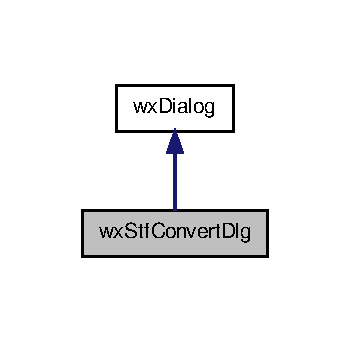
\includegraphics[width=168pt]{classwxStfConvertDlg__inherit__graph}
\end{center}
\end{figure}


Collaboration diagram for wxStfConvertDlg:
\nopagebreak
\begin{figure}[H]
\begin{center}
\leavevmode
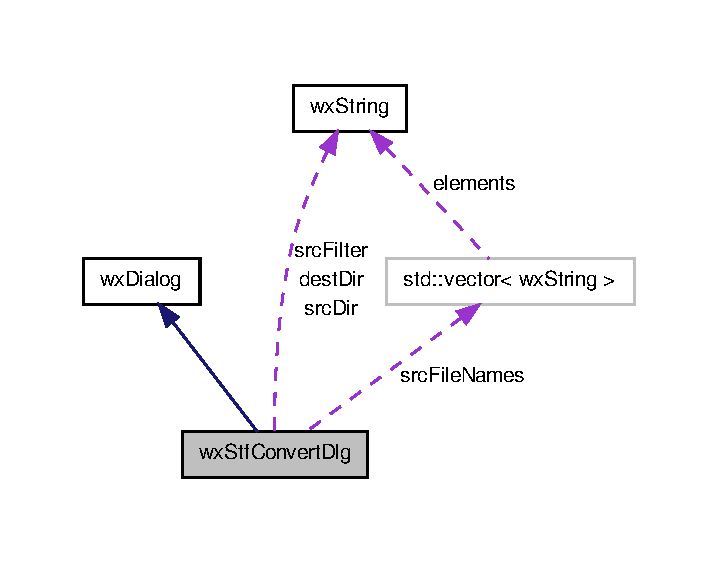
\includegraphics[width=344pt]{classwxStfConvertDlg__coll__graph}
\end{center}
\end{figure}
\subsection*{Public Member Functions}
\begin{DoxyCompactItemize}
\item 
\hyperlink{classwxStfConvertDlg_a1f96707f1cdf3b0e5459ca49bcbc648b}{wxStfConvertDlg} (\hyperlink{classwxWindow}{wxWindow} $\ast$parent, int id=wxID\_\-ANY, \hyperlink{classwxString}{wxString} title=wxT(\char`\"{}Convert CFS files\char`\"{}), wxPoint pos=wxDefaultPosition, \hyperlink{classwxSize}{wxSize} size=wxDefaultSize, int style=wxCAPTION)
\begin{DoxyCompactList}\small\item\em Constructor. \item\end{DoxyCompactList}\item 
\hyperlink{classwxString}{wxString} \hyperlink{classwxStfConvertDlg_addf3c318a648dc3aeb855a2f32416c98}{GetSrcDir} () const 
\begin{DoxyCompactList}\small\item\em Get the source directory. \item\end{DoxyCompactList}\item 
\hyperlink{classwxString}{wxString} \hyperlink{classwxStfConvertDlg_af209dab7add715973cb4efc583e20fa4}{GetDestDir} () const 
\begin{DoxyCompactList}\small\item\em Get the destination directory. \item\end{DoxyCompactList}\item 
\hyperlink{classwxString}{wxString} \hyperlink{classwxStfConvertDlg_a4496190e3ab8965a3fa9d9675881357d}{GetSrcFilter} () const 
\begin{DoxyCompactList}\small\item\em Get the source extension filter. \item\end{DoxyCompactList}\item 
std::vector$<$ \hyperlink{classwxString}{wxString} $>$ \hyperlink{classwxStfConvertDlg_a1fed3038cfba83d7103d2c44ab3d06bd}{GetSrcFileNames} () const 
\begin{DoxyCompactList}\small\item\em Get the list of file names. \item\end{DoxyCompactList}\item 
virtual void \hyperlink{classwxStfConvertDlg_a7271e4bb7b6614f4f3083170564eba8e}{EndModal} (int retCode)
\begin{DoxyCompactList}\small\item\em Called upon ending a modal dialog. \item\end{DoxyCompactList}\end{DoxyCompactItemize}


\subsection{Detailed Description}
Dialog for batch conversion of files.from cfs to atf. 

\subsection{Constructor \& Destructor Documentation}
\hypertarget{classwxStfConvertDlg_a1f96707f1cdf3b0e5459ca49bcbc648b}{
\index{wxStfConvertDlg@{wxStfConvertDlg}!wxStfConvertDlg@{wxStfConvertDlg}}
\index{wxStfConvertDlg@{wxStfConvertDlg}!wxStfConvertDlg@{wxStfConvertDlg}}
\subsubsection[{wxStfConvertDlg}]{\setlength{\rightskip}{0pt plus 5cm}wxStfConvertDlg::wxStfConvertDlg (
\begin{DoxyParamCaption}
\item[{{\bf wxWindow} $\ast$}]{parent, }
\item[{int}]{id = {\ttfamily wxID\_\-ANY}, }
\item[{{\bf wxString}}]{title = {\ttfamily wxT(\char`\"{}Convert~CFS~files\char`\"{})}, }
\item[{{\bf wxPoint}}]{pos = {\ttfamily wxDefaultPosition}, }
\item[{{\bf wxSize}}]{size = {\ttfamily wxDefaultSize}, }
\item[{int}]{style = {\ttfamily wxCAPTION}}
\end{DoxyParamCaption}
)}}
\label{classwxStfConvertDlg_a1f96707f1cdf3b0e5459ca49bcbc648b}


Constructor. 


\begin{DoxyParams}{Parameters}
{\em parent} & Pointer to parent window. \\
\hline
{\em id} & Window id. \\
\hline
{\em title} & Dialog title. \\
\hline
{\em pos} & Initial position. \\
\hline
{\em size} & Initial size. \\
\hline
{\em style} & Dialog style. \\
\hline
\end{DoxyParams}


\subsection{Member Function Documentation}
\hypertarget{classwxStfConvertDlg_a7271e4bb7b6614f4f3083170564eba8e}{
\index{wxStfConvertDlg@{wxStfConvertDlg}!EndModal@{EndModal}}
\index{EndModal@{EndModal}!wxStfConvertDlg@{wxStfConvertDlg}}
\subsubsection[{EndModal}]{\setlength{\rightskip}{0pt plus 5cm}virtual void wxStfConvertDlg::EndModal (
\begin{DoxyParamCaption}
\item[{int}]{retCode}
\end{DoxyParamCaption}
)\hspace{0.3cm}{\ttfamily  \mbox{[}virtual\mbox{]}}}}
\label{classwxStfConvertDlg_a7271e4bb7b6614f4f3083170564eba8e}


Called upon ending a modal dialog. 


\begin{DoxyParams}{Parameters}
{\em retCode} & The dialog button id that ended the dialog (e.g. wxID\_\-OK) \\
\hline
\end{DoxyParams}
\hypertarget{classwxStfConvertDlg_af209dab7add715973cb4efc583e20fa4}{
\index{wxStfConvertDlg@{wxStfConvertDlg}!GetDestDir@{GetDestDir}}
\index{GetDestDir@{GetDestDir}!wxStfConvertDlg@{wxStfConvertDlg}}
\subsubsection[{GetDestDir}]{\setlength{\rightskip}{0pt plus 5cm}{\bf wxString} wxStfConvertDlg::GetDestDir (
\begin{DoxyParamCaption}
{}
\end{DoxyParamCaption}
) const\hspace{0.3cm}{\ttfamily  \mbox{[}inline\mbox{]}}}}
\label{classwxStfConvertDlg_af209dab7add715973cb4efc583e20fa4}


Get the destination directory. 

\begin{DoxyReturn}{Returns}
The destination directory. 
\end{DoxyReturn}
\hypertarget{classwxStfConvertDlg_addf3c318a648dc3aeb855a2f32416c98}{
\index{wxStfConvertDlg@{wxStfConvertDlg}!GetSrcDir@{GetSrcDir}}
\index{GetSrcDir@{GetSrcDir}!wxStfConvertDlg@{wxStfConvertDlg}}
\subsubsection[{GetSrcDir}]{\setlength{\rightskip}{0pt plus 5cm}{\bf wxString} wxStfConvertDlg::GetSrcDir (
\begin{DoxyParamCaption}
{}
\end{DoxyParamCaption}
) const\hspace{0.3cm}{\ttfamily  \mbox{[}inline\mbox{]}}}}
\label{classwxStfConvertDlg_addf3c318a648dc3aeb855a2f32416c98}


Get the source directory. 

\begin{DoxyReturn}{Returns}
The source directory. 
\end{DoxyReturn}
\hypertarget{classwxStfConvertDlg_a1fed3038cfba83d7103d2c44ab3d06bd}{
\index{wxStfConvertDlg@{wxStfConvertDlg}!GetSrcFileNames@{GetSrcFileNames}}
\index{GetSrcFileNames@{GetSrcFileNames}!wxStfConvertDlg@{wxStfConvertDlg}}
\subsubsection[{GetSrcFileNames}]{\setlength{\rightskip}{0pt plus 5cm}std::vector$<${\bf wxString}$>$ wxStfConvertDlg::GetSrcFileNames (
\begin{DoxyParamCaption}
{}
\end{DoxyParamCaption}
) const\hspace{0.3cm}{\ttfamily  \mbox{[}inline\mbox{]}}}}
\label{classwxStfConvertDlg_a1fed3038cfba83d7103d2c44ab3d06bd}


Get the list of file names. 

\begin{DoxyReturn}{Returns}
A vector with source file names. 
\end{DoxyReturn}
\hypertarget{classwxStfConvertDlg_a4496190e3ab8965a3fa9d9675881357d}{
\index{wxStfConvertDlg@{wxStfConvertDlg}!GetSrcFilter@{GetSrcFilter}}
\index{GetSrcFilter@{GetSrcFilter}!wxStfConvertDlg@{wxStfConvertDlg}}
\subsubsection[{GetSrcFilter}]{\setlength{\rightskip}{0pt plus 5cm}{\bf wxString} wxStfConvertDlg::GetSrcFilter (
\begin{DoxyParamCaption}
{}
\end{DoxyParamCaption}
) const\hspace{0.3cm}{\ttfamily  \mbox{[}inline\mbox{]}}}}
\label{classwxStfConvertDlg_a4496190e3ab8965a3fa9d9675881357d}


Get the source extension filter. 

\begin{DoxyReturn}{Returns}
The source extension filter. 
\end{DoxyReturn}


The documentation for this class was generated from the following file:\begin{DoxyCompactItemize}
\item 
src/app/dlgs/\hyperlink{smalldlgs_8h}{smalldlgs.h}\end{DoxyCompactItemize}

\hypertarget{classwxStfCursorsDlg}{
\section{wxStfCursorsDlg Class Reference}
\label{classwxStfCursorsDlg}\index{wxStfCursorsDlg@{wxStfCursorsDlg}}
}


Cursor settings non-\/modal dialog.  




{\ttfamily \#include $<$cursorsdlg.h$>$}



Inheritance diagram for wxStfCursorsDlg:
\nopagebreak
\begin{figure}[H]
\begin{center}
\leavevmode
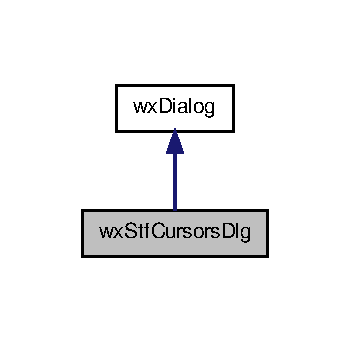
\includegraphics[width=168pt]{classwxStfCursorsDlg__inherit__graph}
\end{center}
\end{figure}


Collaboration diagram for wxStfCursorsDlg:
\nopagebreak
\begin{figure}[H]
\begin{center}
\leavevmode
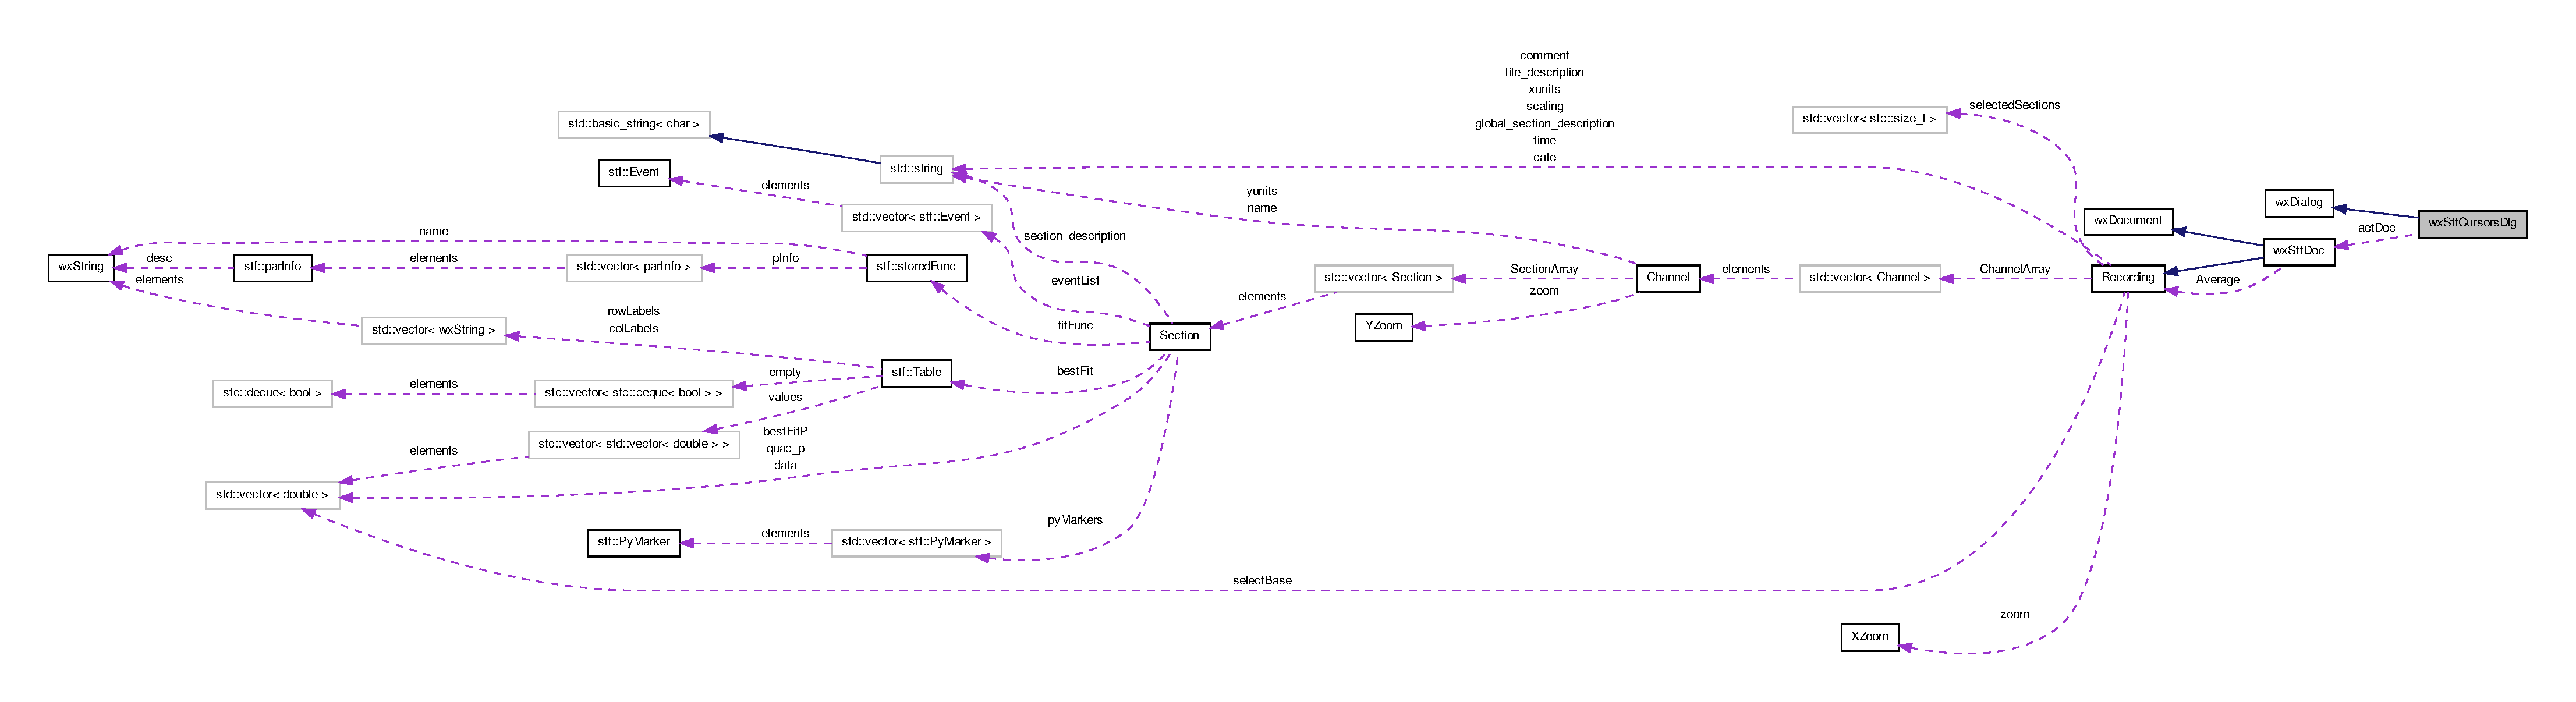
\includegraphics[width=400pt]{classwxStfCursorsDlg__coll__graph}
\end{center}
\end{figure}
\subsection*{Public Member Functions}
\begin{DoxyCompactItemize}
\item 
\hyperlink{classwxStfCursorsDlg_a94b84498bba9d335ecab89e0f5030e41}{wxStfCursorsDlg} (\hyperlink{classwxWindow}{wxWindow} $\ast$parent, \hyperlink{classwxStfDoc}{wxStfDoc} $\ast$initDoc, int id=wxID\_\-ANY, \hyperlink{classwxString}{wxString} title=wxT(\char`\"{}Cursor settings\char`\"{}), wxPoint pos=wxDefaultPosition, \hyperlink{classwxSize}{wxSize} size=wxDefaultSize, int style=wxCAPTION)
\begin{DoxyCompactList}\small\item\em Constructor. \item\end{DoxyCompactList}\item 
virtual void \hyperlink{classwxStfCursorsDlg_afa2eeb514962a88b822018daa4cf84b4}{EndModal} (int retCode)
\begin{DoxyCompactList}\small\item\em Called upon ending a modal dialog. \item\end{DoxyCompactList}\item 
virtual bool \hyperlink{classwxStfCursorsDlg_a681f5abeb01d02fe312a2a164769d98c}{TransferDataFromWindow} ()
\begin{DoxyCompactList}\small\item\em Called when data should be transferred from the non-\/modal dialog (e.g. when OK is pressed) \item\end{DoxyCompactList}\item 
int \hyperlink{classwxStfCursorsDlg_a3c33644d6e71ff2f94c3e2a95889d5a0}{GetCursorM} () const 
\begin{DoxyCompactList}\small\item\em Get the measurement cursor x-\/position. \item\end{DoxyCompactList}\item 
int \hyperlink{classwxStfCursorsDlg_a588a9bc27f41358b26daa1ea7bb9ae53}{GetCursor1P} () const 
\begin{DoxyCompactList}\small\item\em Get the left peak cursor x-\/position. \item\end{DoxyCompactList}\item 
int \hyperlink{classwxStfCursorsDlg_a554f804d5baa56a0a37adb036633db8e}{GetCursor2P} () const 
\begin{DoxyCompactList}\small\item\em Get the right peak cursor x-\/position. \item\end{DoxyCompactList}\item 
int \hyperlink{classwxStfCursorsDlg_a4580524b0a8eab02f773f9d1143f0f31}{GetCursor1B} () const 
\begin{DoxyCompactList}\small\item\em Get the left base cursor x-\/position. \item\end{DoxyCompactList}\item 
int \hyperlink{classwxStfCursorsDlg_af6ecc16a7642f2600d1ff26c0725fed5}{GetCursor2B} () const 
\begin{DoxyCompactList}\small\item\em Get the right base cursor x-\/position. \item\end{DoxyCompactList}\item 
int \hyperlink{classwxStfCursorsDlg_a5ded86530ce6603ccc150c2d7eff2f72}{GetCursor1D} () const 
\begin{DoxyCompactList}\small\item\em Get the left fit cursor x-\/position. \item\end{DoxyCompactList}\item 
int \hyperlink{classwxStfCursorsDlg_abd4e5afc85fbaa1bcb9f1a157781ee99}{GetCursor2D} () const 
\begin{DoxyCompactList}\small\item\em Get the right fit cursor x-\/position. \item\end{DoxyCompactList}\item 
int \hyperlink{classwxStfCursorsDlg_aa66c4a6d63fa6846e281d4810554a31e}{GetCursor1L} () const 
\begin{DoxyCompactList}\small\item\em Get the left latency cursor x-\/position. \item\end{DoxyCompactList}\item 
int \hyperlink{classwxStfCursorsDlg_a2cdeaf3197df8ccf5fe22d7ad57a1719}{GetCursor2L} () const 
\begin{DoxyCompactList}\small\item\em Get the right latency cursor x-\/position. \item\end{DoxyCompactList}\item 
int \hyperlink{classwxStfCursorsDlg_aed1c8d75410af56a4dfba76dae6e2ecc}{GetPeakPoints} () const 
\begin{DoxyCompactList}\small\item\em Gets the number of points used for the binned average during peak detection. \item\end{DoxyCompactList}\item 
void \hyperlink{classwxStfCursorsDlg_a10fdc48de32be164e70eaf49d43c724f}{SetPeakPoints} (int peakPoints)
\begin{DoxyCompactList}\small\item\em Sets the number of points used for the binned average during peak detection. \item\end{DoxyCompactList}\item 
int \hyperlink{classwxStfCursorsDlg_a45576f19bb75432ede2a5743efc38c55}{GetDeltaT} () const 
\begin{DoxyCompactList}\small\item\em Gets the distance to the first PSlope cursor in number of points. \item\end{DoxyCompactList}\item 
void \hyperlink{classwxStfCursorsDlg_a1691b68e582e2bf940f04fd59c2da654}{SetDeltaT} (int DeltaT)
\begin{DoxyCompactList}\small\item\em Sets the number of points used for the distance from the first PSlope cursor. \item\end{DoxyCompactList}\item 
\hyperlink{group__stfgen_gae8845ae2aeaf4b742a905a2a5571fd5a}{stf::direction} \hyperlink{classwxStfCursorsDlg_aebe08375891c206922c3fb9482593964}{GetDirection} () const 
\begin{DoxyCompactList}\small\item\em Gets the direction of peak calculations. \item\end{DoxyCompactList}\item 
\hyperlink{group__stfgen_ga738f9934a45a9d2d81cb0a3de0375c99}{stf::latency\_\-mode} \hyperlink{classwxStfCursorsDlg_ae5c3f8ba6105aaee9f3d4961ba66b962}{GetLatencyStartMode} () const 
\begin{DoxyCompactList}\small\item\em Gets the mode of Latency for the beginning of the latency cursor. \item\end{DoxyCompactList}\item 
\hyperlink{group__stfgen_ga738f9934a45a9d2d81cb0a3de0375c99}{stf::latency\_\-mode} \hyperlink{classwxStfCursorsDlg_a7cfc9e0616e262dfa115345b6afc16de}{GetLatencyEndMode} () const 
\begin{DoxyCompactList}\small\item\em Gets the mode of Latency of the last latency cursor. \item\end{DoxyCompactList}\item 
void \hyperlink{classwxStfCursorsDlg_a79ec551af76845fbf2b07058f3480845}{SetLatencyStartMode} (\hyperlink{group__stfgen_ga738f9934a45a9d2d81cb0a3de0375c99}{stf::latency\_\-mode} latencyBegMode)
\begin{DoxyCompactList}\small\item\em Sets the latency mode of the left latency cursor. \item\end{DoxyCompactList}\item 
void \hyperlink{classwxStfCursorsDlg_a6677d9880b2a68bcb7ffed7ad7a8871a}{SetLatencyEndMode} (\hyperlink{group__stfgen_ga738f9934a45a9d2d81cb0a3de0375c99}{stf::latency\_\-mode} latencyEndMode)
\begin{DoxyCompactList}\small\item\em Sets the latency mode of the right latency cursor. \item\end{DoxyCompactList}\item 
bool \hyperlink{classwxStfCursorsDlg_a8096e588bbd449ede67a15821d3cb34f}{GetFromBase} () const 
\begin{DoxyCompactList}\small\item\em Indicates whether to use the baseline as a reference for AP kinetics. \item\end{DoxyCompactList}\item 
void \hyperlink{classwxStfCursorsDlg_afec8b402c6f0d51d563c63e26aaf00ac}{SetDirection} (\hyperlink{group__stfgen_gae8845ae2aeaf4b742a905a2a5571fd5a}{stf::direction} direction)
\begin{DoxyCompactList}\small\item\em Sets the direction of peak calculations. \item\end{DoxyCompactList}\item 
void \hyperlink{classwxStfCursorsDlg_a9a6b329f076ae3c1e50309c5a6c79a5c}{SetFromBase} (bool frombase)
\begin{DoxyCompactList}\small\item\em Sets the reference for AP kinetics measurements. \item\end{DoxyCompactList}\item 
bool \hyperlink{classwxStfCursorsDlg_ae1579db95062fd20394a498bfd3dc924}{GetPeakAtEnd} () const 
\begin{DoxyCompactList}\small\item\em Indicates whether the right peak cursor should always be at the end of the trace. \item\end{DoxyCompactList}\item 
bool \hyperlink{classwxStfCursorsDlg_aa6d011bfe921c1d038b720fb7c94a3ec}{GetStartFitAtPeak} () const 
\begin{DoxyCompactList}\small\item\em Indicates whether to always start a fit at the current peak position. \item\end{DoxyCompactList}\item 
\hypertarget{classwxStfCursorsDlg_a299bb15e4c37376c620e71dac269d6a5}{
void \hyperlink{classwxStfCursorsDlg_a299bb15e4c37376c620e71dac269d6a5}{UpdateCursors} ()}
\label{classwxStfCursorsDlg_a299bb15e4c37376c620e71dac269d6a5}

\begin{DoxyCompactList}\small\item\em Updates the cursor entries in the Cursors Settings menu. \item\end{DoxyCompactList}\item 
\hyperlink{group__stfgen_gad2d1acb3ac0c16ee32b5f4d3a1ab4abf}{stf::cursor\_\-type} \hyperlink{classwxStfCursorsDlg_a2fe14dd421b1df3d14c7fba062bb56a8}{CurrentCursor} () const 
\begin{DoxyCompactList}\small\item\em Retrieve the current cursor notebook page. \item\end{DoxyCompactList}\item 
double \hyperlink{classwxStfCursorsDlg_a24a5953757bb1883724c18088a65b380}{GetSlope} () const 
\begin{DoxyCompactList}\small\item\em Get the slope at which the baseline should be fixed. \item\end{DoxyCompactList}\item 
void \hyperlink{classwxStfCursorsDlg_ad761357b9b82e1e9ffa3bd70a7dca671}{SetSlope} (double slope)
\begin{DoxyCompactList}\small\item\em Set the threshold slope. \item\end{DoxyCompactList}\item 
void \hyperlink{classwxStfCursorsDlg_ad6d4fd19849612abd62db33ede3d3ca6}{SetSlopeUnits} (const \hyperlink{classwxString}{wxString} \&units)
\begin{DoxyCompactList}\small\item\em Set the units of the slope. \item\end{DoxyCompactList}\item 
bool \hyperlink{classwxStfCursorsDlg_a52bed6f2df9a325990130f1958de9d37}{GetBaseToSlope} () const 
\begin{DoxyCompactList}\small\item\em Indicates whether the baseline should be fixed to a certain slope. \item\end{DoxyCompactList}\item 
bool \hyperlink{classwxStfCursorsDlg_a000170c56fe7f09dc830f89031fc6e4c}{GetRuler} () const 
\begin{DoxyCompactList}\small\item\em Indicates whether an additional vertical ruler should be drawn through the baseline. \item\end{DoxyCompactList}\item 
void \hyperlink{classwxStfCursorsDlg_a32207ff701a636525f6cb1e4ac8852f6}{SetActiveDoc} (\hyperlink{classwxStfDoc}{wxStfDoc} $\ast$actDoc\_\-)
\begin{DoxyCompactList}\small\item\em Sets the currently active document. \item\end{DoxyCompactList}\end{DoxyCompactItemize}


\subsection{Detailed Description}
Cursor settings non-\/modal dialog. 

\subsection{Constructor \& Destructor Documentation}
\hypertarget{classwxStfCursorsDlg_a94b84498bba9d335ecab89e0f5030e41}{
\index{wxStfCursorsDlg@{wxStfCursorsDlg}!wxStfCursorsDlg@{wxStfCursorsDlg}}
\index{wxStfCursorsDlg@{wxStfCursorsDlg}!wxStfCursorsDlg@{wxStfCursorsDlg}}
\subsubsection[{wxStfCursorsDlg}]{\setlength{\rightskip}{0pt plus 5cm}wxStfCursorsDlg::wxStfCursorsDlg (
\begin{DoxyParamCaption}
\item[{{\bf wxWindow} $\ast$}]{parent, }
\item[{{\bf wxStfDoc} $\ast$}]{initDoc, }
\item[{int}]{id = {\ttfamily wxID\_\-ANY}, }
\item[{{\bf wxString}}]{title = {\ttfamily wxT(\char`\"{}Cursor~settings\char`\"{})}, }
\item[{{\bf wxPoint}}]{pos = {\ttfamily wxDefaultPosition}, }
\item[{{\bf wxSize}}]{size = {\ttfamily wxDefaultSize}, }
\item[{int}]{style = {\ttfamily wxCAPTION}}
\end{DoxyParamCaption}
)}}
\label{classwxStfCursorsDlg_a94b84498bba9d335ecab89e0f5030e41}


Constructor. 


\begin{DoxyParams}{Parameters}
{\em parent} & Pointer to parent window. \\
\hline
{\em initDoc} & Pointer to the document the call originated from. \\
\hline
{\em id} & Window id. \\
\hline
{\em title} & Dialog title. \\
\hline
{\em pos} & Initial position. \\
\hline
{\em size} & Initial size. \\
\hline
{\em style} & Dialog style. \\
\hline
\end{DoxyParams}


\subsection{Member Function Documentation}
\hypertarget{classwxStfCursorsDlg_a2fe14dd421b1df3d14c7fba062bb56a8}{
\index{wxStfCursorsDlg@{wxStfCursorsDlg}!CurrentCursor@{CurrentCursor}}
\index{CurrentCursor@{CurrentCursor}!wxStfCursorsDlg@{wxStfCursorsDlg}}
\subsubsection[{CurrentCursor}]{\setlength{\rightskip}{0pt plus 5cm}{\bf stf::cursor\_\-type} wxStfCursorsDlg::CurrentCursor (
\begin{DoxyParamCaption}
{}
\end{DoxyParamCaption}
) const}}
\label{classwxStfCursorsDlg_a2fe14dd421b1df3d14c7fba062bb56a8}


Retrieve the current cursor notebook page. 

\begin{DoxyReturn}{Returns}
The cursor corresponding to the currently selected notebook page. 
\end{DoxyReturn}
\hypertarget{classwxStfCursorsDlg_afa2eeb514962a88b822018daa4cf84b4}{
\index{wxStfCursorsDlg@{wxStfCursorsDlg}!EndModal@{EndModal}}
\index{EndModal@{EndModal}!wxStfCursorsDlg@{wxStfCursorsDlg}}
\subsubsection[{EndModal}]{\setlength{\rightskip}{0pt plus 5cm}virtual void wxStfCursorsDlg::EndModal (
\begin{DoxyParamCaption}
\item[{int}]{retCode}
\end{DoxyParamCaption}
)\hspace{0.3cm}{\ttfamily  \mbox{[}virtual\mbox{]}}}}
\label{classwxStfCursorsDlg_afa2eeb514962a88b822018daa4cf84b4}


Called upon ending a modal dialog. 


\begin{DoxyParams}{Parameters}
{\em retCode} & The dialog button id that ended the dialog (e.g. wxID\_\-OK) \\
\hline
\end{DoxyParams}
\hypertarget{classwxStfCursorsDlg_a52bed6f2df9a325990130f1958de9d37}{
\index{wxStfCursorsDlg@{wxStfCursorsDlg}!GetBaseToSlope@{GetBaseToSlope}}
\index{GetBaseToSlope@{GetBaseToSlope}!wxStfCursorsDlg@{wxStfCursorsDlg}}
\subsubsection[{GetBaseToSlope}]{\setlength{\rightskip}{0pt plus 5cm}bool wxStfCursorsDlg::GetBaseToSlope (
\begin{DoxyParamCaption}
{}
\end{DoxyParamCaption}
) const}}
\label{classwxStfCursorsDlg_a52bed6f2df9a325990130f1958de9d37}


Indicates whether the baseline should be fixed to a certain slope. 

\begin{DoxyReturn}{Returns}
true if the baseline should be fixed, false otherwise. 
\end{DoxyReturn}
\hypertarget{classwxStfCursorsDlg_a4580524b0a8eab02f773f9d1143f0f31}{
\index{wxStfCursorsDlg@{wxStfCursorsDlg}!GetCursor1B@{GetCursor1B}}
\index{GetCursor1B@{GetCursor1B}!wxStfCursorsDlg@{wxStfCursorsDlg}}
\subsubsection[{GetCursor1B}]{\setlength{\rightskip}{0pt plus 5cm}int wxStfCursorsDlg::GetCursor1B (
\begin{DoxyParamCaption}
{}
\end{DoxyParamCaption}
) const}}
\label{classwxStfCursorsDlg_a4580524b0a8eab02f773f9d1143f0f31}


Get the left base cursor x-\/position. 

\begin{DoxyReturn}{Returns}
The left base cursor x-\/position in units of sampling points. 
\end{DoxyReturn}
\hypertarget{classwxStfCursorsDlg_a5ded86530ce6603ccc150c2d7eff2f72}{
\index{wxStfCursorsDlg@{wxStfCursorsDlg}!GetCursor1D@{GetCursor1D}}
\index{GetCursor1D@{GetCursor1D}!wxStfCursorsDlg@{wxStfCursorsDlg}}
\subsubsection[{GetCursor1D}]{\setlength{\rightskip}{0pt plus 5cm}int wxStfCursorsDlg::GetCursor1D (
\begin{DoxyParamCaption}
{}
\end{DoxyParamCaption}
) const}}
\label{classwxStfCursorsDlg_a5ded86530ce6603ccc150c2d7eff2f72}


Get the left fit cursor x-\/position. 

\begin{DoxyReturn}{Returns}
The left fit cursor x-\/position in units of sampling points. 
\end{DoxyReturn}
\hypertarget{classwxStfCursorsDlg_aa66c4a6d63fa6846e281d4810554a31e}{
\index{wxStfCursorsDlg@{wxStfCursorsDlg}!GetCursor1L@{GetCursor1L}}
\index{GetCursor1L@{GetCursor1L}!wxStfCursorsDlg@{wxStfCursorsDlg}}
\subsubsection[{GetCursor1L}]{\setlength{\rightskip}{0pt plus 5cm}int wxStfCursorsDlg::GetCursor1L (
\begin{DoxyParamCaption}
{}
\end{DoxyParamCaption}
) const}}
\label{classwxStfCursorsDlg_aa66c4a6d63fa6846e281d4810554a31e}


Get the left latency cursor x-\/position. 

\begin{DoxyReturn}{Returns}
The left fit cursor x-\/position in units of sampling points. 
\end{DoxyReturn}
\hypertarget{classwxStfCursorsDlg_a588a9bc27f41358b26daa1ea7bb9ae53}{
\index{wxStfCursorsDlg@{wxStfCursorsDlg}!GetCursor1P@{GetCursor1P}}
\index{GetCursor1P@{GetCursor1P}!wxStfCursorsDlg@{wxStfCursorsDlg}}
\subsubsection[{GetCursor1P}]{\setlength{\rightskip}{0pt plus 5cm}int wxStfCursorsDlg::GetCursor1P (
\begin{DoxyParamCaption}
{}
\end{DoxyParamCaption}
) const}}
\label{classwxStfCursorsDlg_a588a9bc27f41358b26daa1ea7bb9ae53}


Get the left peak cursor x-\/position. 

\begin{DoxyReturn}{Returns}
The left peak cursor x-\/position in units of sampling points. 
\end{DoxyReturn}
\hypertarget{classwxStfCursorsDlg_af6ecc16a7642f2600d1ff26c0725fed5}{
\index{wxStfCursorsDlg@{wxStfCursorsDlg}!GetCursor2B@{GetCursor2B}}
\index{GetCursor2B@{GetCursor2B}!wxStfCursorsDlg@{wxStfCursorsDlg}}
\subsubsection[{GetCursor2B}]{\setlength{\rightskip}{0pt plus 5cm}int wxStfCursorsDlg::GetCursor2B (
\begin{DoxyParamCaption}
{}
\end{DoxyParamCaption}
) const}}
\label{classwxStfCursorsDlg_af6ecc16a7642f2600d1ff26c0725fed5}


Get the right base cursor x-\/position. 

\begin{DoxyReturn}{Returns}
The right base cursor x-\/position in units of sampling points. 
\end{DoxyReturn}
\hypertarget{classwxStfCursorsDlg_abd4e5afc85fbaa1bcb9f1a157781ee99}{
\index{wxStfCursorsDlg@{wxStfCursorsDlg}!GetCursor2D@{GetCursor2D}}
\index{GetCursor2D@{GetCursor2D}!wxStfCursorsDlg@{wxStfCursorsDlg}}
\subsubsection[{GetCursor2D}]{\setlength{\rightskip}{0pt plus 5cm}int wxStfCursorsDlg::GetCursor2D (
\begin{DoxyParamCaption}
{}
\end{DoxyParamCaption}
) const}}
\label{classwxStfCursorsDlg_abd4e5afc85fbaa1bcb9f1a157781ee99}


Get the right fit cursor x-\/position. 

\begin{DoxyReturn}{Returns}
The right fit cursor x-\/position in units of sampling points. 
\end{DoxyReturn}
\hypertarget{classwxStfCursorsDlg_a2cdeaf3197df8ccf5fe22d7ad57a1719}{
\index{wxStfCursorsDlg@{wxStfCursorsDlg}!GetCursor2L@{GetCursor2L}}
\index{GetCursor2L@{GetCursor2L}!wxStfCursorsDlg@{wxStfCursorsDlg}}
\subsubsection[{GetCursor2L}]{\setlength{\rightskip}{0pt plus 5cm}int wxStfCursorsDlg::GetCursor2L (
\begin{DoxyParamCaption}
{}
\end{DoxyParamCaption}
) const}}
\label{classwxStfCursorsDlg_a2cdeaf3197df8ccf5fe22d7ad57a1719}


Get the right latency cursor x-\/position. 

\begin{DoxyReturn}{Returns}
The right fit cursor x-\/position in units of sampling points. 
\end{DoxyReturn}
\hypertarget{classwxStfCursorsDlg_a554f804d5baa56a0a37adb036633db8e}{
\index{wxStfCursorsDlg@{wxStfCursorsDlg}!GetCursor2P@{GetCursor2P}}
\index{GetCursor2P@{GetCursor2P}!wxStfCursorsDlg@{wxStfCursorsDlg}}
\subsubsection[{GetCursor2P}]{\setlength{\rightskip}{0pt plus 5cm}int wxStfCursorsDlg::GetCursor2P (
\begin{DoxyParamCaption}
{}
\end{DoxyParamCaption}
) const}}
\label{classwxStfCursorsDlg_a554f804d5baa56a0a37adb036633db8e}


Get the right peak cursor x-\/position. 

\begin{DoxyReturn}{Returns}
The right peak cursor x-\/position in units of sampling points. 
\end{DoxyReturn}
\hypertarget{classwxStfCursorsDlg_a3c33644d6e71ff2f94c3e2a95889d5a0}{
\index{wxStfCursorsDlg@{wxStfCursorsDlg}!GetCursorM@{GetCursorM}}
\index{GetCursorM@{GetCursorM}!wxStfCursorsDlg@{wxStfCursorsDlg}}
\subsubsection[{GetCursorM}]{\setlength{\rightskip}{0pt plus 5cm}int wxStfCursorsDlg::GetCursorM (
\begin{DoxyParamCaption}
{}
\end{DoxyParamCaption}
) const}}
\label{classwxStfCursorsDlg_a3c33644d6e71ff2f94c3e2a95889d5a0}


Get the measurement cursor x-\/position. 

\begin{DoxyReturn}{Returns}
The measurement cursor x-\/position in units of sampling points. 
\end{DoxyReturn}
\hypertarget{classwxStfCursorsDlg_a45576f19bb75432ede2a5743efc38c55}{
\index{wxStfCursorsDlg@{wxStfCursorsDlg}!GetDeltaT@{GetDeltaT}}
\index{GetDeltaT@{GetDeltaT}!wxStfCursorsDlg@{wxStfCursorsDlg}}
\subsubsection[{GetDeltaT}]{\setlength{\rightskip}{0pt plus 5cm}int wxStfCursorsDlg::GetDeltaT (
\begin{DoxyParamCaption}
{}
\end{DoxyParamCaption}
) const}}
\label{classwxStfCursorsDlg_a45576f19bb75432ede2a5743efc38c55}


Gets the distance to the first PSlope cursor in number of points. 

\begin{DoxyReturn}{Returns}
The distance to the first PSlope cursor in number of points. 
\end{DoxyReturn}
\hypertarget{classwxStfCursorsDlg_aebe08375891c206922c3fb9482593964}{
\index{wxStfCursorsDlg@{wxStfCursorsDlg}!GetDirection@{GetDirection}}
\index{GetDirection@{GetDirection}!wxStfCursorsDlg@{wxStfCursorsDlg}}
\subsubsection[{GetDirection}]{\setlength{\rightskip}{0pt plus 5cm}{\bf stf::direction} wxStfCursorsDlg::GetDirection (
\begin{DoxyParamCaption}
{}
\end{DoxyParamCaption}
) const}}
\label{classwxStfCursorsDlg_aebe08375891c206922c3fb9482593964}


Gets the direction of peak calculations. 

\begin{DoxyReturn}{Returns}
The current direction of peak calculations. 
\end{DoxyReturn}
\hypertarget{classwxStfCursorsDlg_a8096e588bbd449ede67a15821d3cb34f}{
\index{wxStfCursorsDlg@{wxStfCursorsDlg}!GetFromBase@{GetFromBase}}
\index{GetFromBase@{GetFromBase}!wxStfCursorsDlg@{wxStfCursorsDlg}}
\subsubsection[{GetFromBase}]{\setlength{\rightskip}{0pt plus 5cm}bool wxStfCursorsDlg::GetFromBase (
\begin{DoxyParamCaption}
{}
\end{DoxyParamCaption}
) const}}
\label{classwxStfCursorsDlg_a8096e588bbd449ede67a15821d3cb34f}


Indicates whether to use the baseline as a reference for AP kinetics. 

\begin{DoxyReturn}{Returns}
true if the baseline should be used, false if the threshold should be used. 
\end{DoxyReturn}
\hypertarget{classwxStfCursorsDlg_a7cfc9e0616e262dfa115345b6afc16de}{
\index{wxStfCursorsDlg@{wxStfCursorsDlg}!GetLatencyEndMode@{GetLatencyEndMode}}
\index{GetLatencyEndMode@{GetLatencyEndMode}!wxStfCursorsDlg@{wxStfCursorsDlg}}
\subsubsection[{GetLatencyEndMode}]{\setlength{\rightskip}{0pt plus 5cm}{\bf stf::latency\_\-mode} wxStfCursorsDlg::GetLatencyEndMode (
\begin{DoxyParamCaption}
{}
\end{DoxyParamCaption}
) const}}
\label{classwxStfCursorsDlg_a7cfc9e0616e262dfa115345b6afc16de}


Gets the mode of Latency of the last latency cursor. 

\begin{DoxyReturn}{Returns}
The current mode of the last latency cursor. 
\end{DoxyReturn}
\hypertarget{classwxStfCursorsDlg_ae5c3f8ba6105aaee9f3d4961ba66b962}{
\index{wxStfCursorsDlg@{wxStfCursorsDlg}!GetLatencyStartMode@{GetLatencyStartMode}}
\index{GetLatencyStartMode@{GetLatencyStartMode}!wxStfCursorsDlg@{wxStfCursorsDlg}}
\subsubsection[{GetLatencyStartMode}]{\setlength{\rightskip}{0pt plus 5cm}{\bf stf::latency\_\-mode} wxStfCursorsDlg::GetLatencyStartMode (
\begin{DoxyParamCaption}
{}
\end{DoxyParamCaption}
) const}}
\label{classwxStfCursorsDlg_ae5c3f8ba6105aaee9f3d4961ba66b962}


Gets the mode of Latency for the beginning of the latency cursor. 

\begin{DoxyReturn}{Returns}
The current mode for the beginning latency cursor. 
\end{DoxyReturn}
\hypertarget{classwxStfCursorsDlg_ae1579db95062fd20394a498bfd3dc924}{
\index{wxStfCursorsDlg@{wxStfCursorsDlg}!GetPeakAtEnd@{GetPeakAtEnd}}
\index{GetPeakAtEnd@{GetPeakAtEnd}!wxStfCursorsDlg@{wxStfCursorsDlg}}
\subsubsection[{GetPeakAtEnd}]{\setlength{\rightskip}{0pt plus 5cm}bool wxStfCursorsDlg::GetPeakAtEnd (
\begin{DoxyParamCaption}
{}
\end{DoxyParamCaption}
) const}}
\label{classwxStfCursorsDlg_ae1579db95062fd20394a498bfd3dc924}


Indicates whether the right peak cursor should always be at the end of the trace. 

\begin{DoxyReturn}{Returns}
true if the peak cursor should always be at the end of the trace. 
\end{DoxyReturn}
\hypertarget{classwxStfCursorsDlg_aed1c8d75410af56a4dfba76dae6e2ecc}{
\index{wxStfCursorsDlg@{wxStfCursorsDlg}!GetPeakPoints@{GetPeakPoints}}
\index{GetPeakPoints@{GetPeakPoints}!wxStfCursorsDlg@{wxStfCursorsDlg}}
\subsubsection[{GetPeakPoints}]{\setlength{\rightskip}{0pt plus 5cm}int wxStfCursorsDlg::GetPeakPoints (
\begin{DoxyParamCaption}
{}
\end{DoxyParamCaption}
) const}}
\label{classwxStfCursorsDlg_aed1c8d75410af56a4dfba76dae6e2ecc}


Gets the number of points used for the binned average during peak detection. 

\begin{DoxyReturn}{Returns}
The number of points used for the binned average during peak detection. 
\end{DoxyReturn}
\hypertarget{classwxStfCursorsDlg_a000170c56fe7f09dc830f89031fc6e4c}{
\index{wxStfCursorsDlg@{wxStfCursorsDlg}!GetRuler@{GetRuler}}
\index{GetRuler@{GetRuler}!wxStfCursorsDlg@{wxStfCursorsDlg}}
\subsubsection[{GetRuler}]{\setlength{\rightskip}{0pt plus 5cm}bool wxStfCursorsDlg::GetRuler (
\begin{DoxyParamCaption}
{}
\end{DoxyParamCaption}
) const}}
\label{classwxStfCursorsDlg_a000170c56fe7f09dc830f89031fc6e4c}


Indicates whether an additional vertical ruler should be drawn through the baseline. 

\begin{DoxyReturn}{Returns}
true if an additional ruler should be drawn. 
\end{DoxyReturn}
\hypertarget{classwxStfCursorsDlg_a24a5953757bb1883724c18088a65b380}{
\index{wxStfCursorsDlg@{wxStfCursorsDlg}!GetSlope@{GetSlope}}
\index{GetSlope@{GetSlope}!wxStfCursorsDlg@{wxStfCursorsDlg}}
\subsubsection[{GetSlope}]{\setlength{\rightskip}{0pt plus 5cm}double wxStfCursorsDlg::GetSlope (
\begin{DoxyParamCaption}
{}
\end{DoxyParamCaption}
) const}}
\label{classwxStfCursorsDlg_a24a5953757bb1883724c18088a65b380}


Get the slope at which the baseline should be fixed. 

\begin{DoxyReturn}{Returns}
The slope at which the baseline should be fixed. 
\end{DoxyReturn}
\hypertarget{classwxStfCursorsDlg_aa6d011bfe921c1d038b720fb7c94a3ec}{
\index{wxStfCursorsDlg@{wxStfCursorsDlg}!GetStartFitAtPeak@{GetStartFitAtPeak}}
\index{GetStartFitAtPeak@{GetStartFitAtPeak}!wxStfCursorsDlg@{wxStfCursorsDlg}}
\subsubsection[{GetStartFitAtPeak}]{\setlength{\rightskip}{0pt plus 5cm}bool wxStfCursorsDlg::GetStartFitAtPeak (
\begin{DoxyParamCaption}
{}
\end{DoxyParamCaption}
) const}}
\label{classwxStfCursorsDlg_aa6d011bfe921c1d038b720fb7c94a3ec}


Indicates whether to always start a fit at the current peak position. 

\begin{DoxyReturn}{Returns}
true if the fit should always be started at the current peak position. 
\end{DoxyReturn}
\hypertarget{classwxStfCursorsDlg_a32207ff701a636525f6cb1e4ac8852f6}{
\index{wxStfCursorsDlg@{wxStfCursorsDlg}!SetActiveDoc@{SetActiveDoc}}
\index{SetActiveDoc@{SetActiveDoc}!wxStfCursorsDlg@{wxStfCursorsDlg}}
\subsubsection[{SetActiveDoc}]{\setlength{\rightskip}{0pt plus 5cm}void wxStfCursorsDlg::SetActiveDoc (
\begin{DoxyParamCaption}
\item[{{\bf wxStfDoc} $\ast$}]{actDoc\_\-}
\end{DoxyParamCaption}
)\hspace{0.3cm}{\ttfamily  \mbox{[}inline\mbox{]}}}}
\label{classwxStfCursorsDlg_a32207ff701a636525f6cb1e4ac8852f6}


Sets the currently active document. 


\begin{DoxyParams}{Parameters}
{\em actDoc\_\-} & A pointer to the currently active document. \\
\hline
\end{DoxyParams}
\hypertarget{classwxStfCursorsDlg_a1691b68e582e2bf940f04fd59c2da654}{
\index{wxStfCursorsDlg@{wxStfCursorsDlg}!SetDeltaT@{SetDeltaT}}
\index{SetDeltaT@{SetDeltaT}!wxStfCursorsDlg@{wxStfCursorsDlg}}
\subsubsection[{SetDeltaT}]{\setlength{\rightskip}{0pt plus 5cm}void wxStfCursorsDlg::SetDeltaT (
\begin{DoxyParamCaption}
\item[{int}]{DeltaT}
\end{DoxyParamCaption}
)}}
\label{classwxStfCursorsDlg_a1691b68e582e2bf940f04fd59c2da654}


Sets the number of points used for the distance from the first PSlope cursor. 


\begin{DoxyParams}{Parameters}
{\em peakPoints} & The number of points used for the distance from the first PSlope cursor. \\
\hline
\end{DoxyParams}
\hypertarget{classwxStfCursorsDlg_afec8b402c6f0d51d563c63e26aaf00ac}{
\index{wxStfCursorsDlg@{wxStfCursorsDlg}!SetDirection@{SetDirection}}
\index{SetDirection@{SetDirection}!wxStfCursorsDlg@{wxStfCursorsDlg}}
\subsubsection[{SetDirection}]{\setlength{\rightskip}{0pt plus 5cm}void wxStfCursorsDlg::SetDirection (
\begin{DoxyParamCaption}
\item[{{\bf stf::direction}}]{direction}
\end{DoxyParamCaption}
)}}
\label{classwxStfCursorsDlg_afec8b402c6f0d51d563c63e26aaf00ac}


Sets the direction of peak calculations. 


\begin{DoxyParams}{Parameters}
{\em direction} & The new direction of peak calculations. \\
\hline
\end{DoxyParams}
\hypertarget{classwxStfCursorsDlg_a9a6b329f076ae3c1e50309c5a6c79a5c}{
\index{wxStfCursorsDlg@{wxStfCursorsDlg}!SetFromBase@{SetFromBase}}
\index{SetFromBase@{SetFromBase}!wxStfCursorsDlg@{wxStfCursorsDlg}}
\subsubsection[{SetFromBase}]{\setlength{\rightskip}{0pt plus 5cm}void wxStfCursorsDlg::SetFromBase (
\begin{DoxyParamCaption}
\item[{bool}]{frombase}
\end{DoxyParamCaption}
)}}
\label{classwxStfCursorsDlg_a9a6b329f076ae3c1e50309c5a6c79a5c}


Sets the reference for AP kinetics measurements. 


\begin{DoxyParams}{Parameters}
{\em frombase} & true if the baseline should be used, false if the threshold should be used. \\
\hline
\end{DoxyParams}
\hypertarget{classwxStfCursorsDlg_a6677d9880b2a68bcb7ffed7ad7a8871a}{
\index{wxStfCursorsDlg@{wxStfCursorsDlg}!SetLatencyEndMode@{SetLatencyEndMode}}
\index{SetLatencyEndMode@{SetLatencyEndMode}!wxStfCursorsDlg@{wxStfCursorsDlg}}
\subsubsection[{SetLatencyEndMode}]{\setlength{\rightskip}{0pt plus 5cm}void wxStfCursorsDlg::SetLatencyEndMode (
\begin{DoxyParamCaption}
\item[{{\bf stf::latency\_\-mode}}]{latencyEndMode}
\end{DoxyParamCaption}
)}}
\label{classwxStfCursorsDlg_a6677d9880b2a68bcb7ffed7ad7a8871a}


Sets the latency mode of the right latency cursor. 


\begin{DoxyParams}{Parameters}
{\em latencyEndMode,:} & the new mode for the right latency cursor. \\
\hline
\end{DoxyParams}
\hypertarget{classwxStfCursorsDlg_a79ec551af76845fbf2b07058f3480845}{
\index{wxStfCursorsDlg@{wxStfCursorsDlg}!SetLatencyStartMode@{SetLatencyStartMode}}
\index{SetLatencyStartMode@{SetLatencyStartMode}!wxStfCursorsDlg@{wxStfCursorsDlg}}
\subsubsection[{SetLatencyStartMode}]{\setlength{\rightskip}{0pt plus 5cm}void wxStfCursorsDlg::SetLatencyStartMode (
\begin{DoxyParamCaption}
\item[{{\bf stf::latency\_\-mode}}]{latencyBegMode}
\end{DoxyParamCaption}
)}}
\label{classwxStfCursorsDlg_a79ec551af76845fbf2b07058f3480845}


Sets the latency mode of the left latency cursor. 


\begin{DoxyParams}{Parameters}
{\em latencyBegMode,:} & the new mode for the left latency cursor. \\
\hline
\end{DoxyParams}
\hypertarget{classwxStfCursorsDlg_a10fdc48de32be164e70eaf49d43c724f}{
\index{wxStfCursorsDlg@{wxStfCursorsDlg}!SetPeakPoints@{SetPeakPoints}}
\index{SetPeakPoints@{SetPeakPoints}!wxStfCursorsDlg@{wxStfCursorsDlg}}
\subsubsection[{SetPeakPoints}]{\setlength{\rightskip}{0pt plus 5cm}void wxStfCursorsDlg::SetPeakPoints (
\begin{DoxyParamCaption}
\item[{int}]{peakPoints}
\end{DoxyParamCaption}
)}}
\label{classwxStfCursorsDlg_a10fdc48de32be164e70eaf49d43c724f}


Sets the number of points used for the binned average during peak detection. 


\begin{DoxyParams}{Parameters}
{\em peakPoints} & The number of points used for the binned average during peak detection. \\
\hline
\end{DoxyParams}
\hypertarget{classwxStfCursorsDlg_ad761357b9b82e1e9ffa3bd70a7dca671}{
\index{wxStfCursorsDlg@{wxStfCursorsDlg}!SetSlope@{SetSlope}}
\index{SetSlope@{SetSlope}!wxStfCursorsDlg@{wxStfCursorsDlg}}
\subsubsection[{SetSlope}]{\setlength{\rightskip}{0pt plus 5cm}void wxStfCursorsDlg::SetSlope (
\begin{DoxyParamCaption}
\item[{double}]{slope}
\end{DoxyParamCaption}
)}}
\label{classwxStfCursorsDlg_ad761357b9b82e1e9ffa3bd70a7dca671}


Set the threshold slope. 


\begin{DoxyParams}{Parameters}
{\em slope} & The new threshold slope. \\
\hline
\end{DoxyParams}
\hypertarget{classwxStfCursorsDlg_ad6d4fd19849612abd62db33ede3d3ca6}{
\index{wxStfCursorsDlg@{wxStfCursorsDlg}!SetSlopeUnits@{SetSlopeUnits}}
\index{SetSlopeUnits@{SetSlopeUnits}!wxStfCursorsDlg@{wxStfCursorsDlg}}
\subsubsection[{SetSlopeUnits}]{\setlength{\rightskip}{0pt plus 5cm}void wxStfCursorsDlg::SetSlopeUnits (
\begin{DoxyParamCaption}
\item[{const {\bf wxString} \&}]{units}
\end{DoxyParamCaption}
)}}
\label{classwxStfCursorsDlg_ad6d4fd19849612abd62db33ede3d3ca6}


Set the units of the slope. 


\begin{DoxyParams}{Parameters}
{\em units} & The units of the slope. \\
\hline
\end{DoxyParams}
\hypertarget{classwxStfCursorsDlg_a681f5abeb01d02fe312a2a164769d98c}{
\index{wxStfCursorsDlg@{wxStfCursorsDlg}!TransferDataFromWindow@{TransferDataFromWindow}}
\index{TransferDataFromWindow@{TransferDataFromWindow}!wxStfCursorsDlg@{wxStfCursorsDlg}}
\subsubsection[{TransferDataFromWindow}]{\setlength{\rightskip}{0pt plus 5cm}virtual bool wxStfCursorsDlg::TransferDataFromWindow (
\begin{DoxyParamCaption}
{}
\end{DoxyParamCaption}
)\hspace{0.3cm}{\ttfamily  \mbox{[}virtual\mbox{]}}}}
\label{classwxStfCursorsDlg_a681f5abeb01d02fe312a2a164769d98c}


Called when data should be transferred from the non-\/modal dialog (e.g. when OK is pressed) 

Note that a non-\/modal dialog won't be destroyed when OK is clicked, it will only disappear from sight. This function will then apply the current cursor settings and update the results table. \begin{DoxyReturn}{Returns}
The return value of the base class version wxWindow::TransferDataFromWindow() 
\end{DoxyReturn}


The documentation for this class was generated from the following file:\begin{DoxyCompactItemize}
\item 
src/app/dlgs/\hyperlink{cursorsdlg_8h}{cursorsdlg.h}\end{DoxyCompactItemize}

\hypertarget{classwxStfDoc}{
\section{wxStfDoc Class Reference}
\label{classwxStfDoc}\index{wxStfDoc@{wxStfDoc}}
}


The document class, derived from both \hyperlink{classwxDocument}{wxDocument} and \hyperlink{classRecording}{Recording}.  




{\ttfamily \#include $<$doc.h$>$}



Inheritance diagram for wxStfDoc:
\nopagebreak
\begin{figure}[H]
\begin{center}
\leavevmode
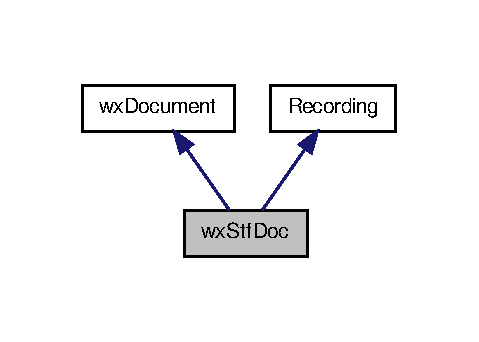
\includegraphics[width=230pt]{classwxStfDoc__inherit__graph}
\end{center}
\end{figure}


Collaboration diagram for wxStfDoc:
\nopagebreak
\begin{figure}[H]
\begin{center}
\leavevmode
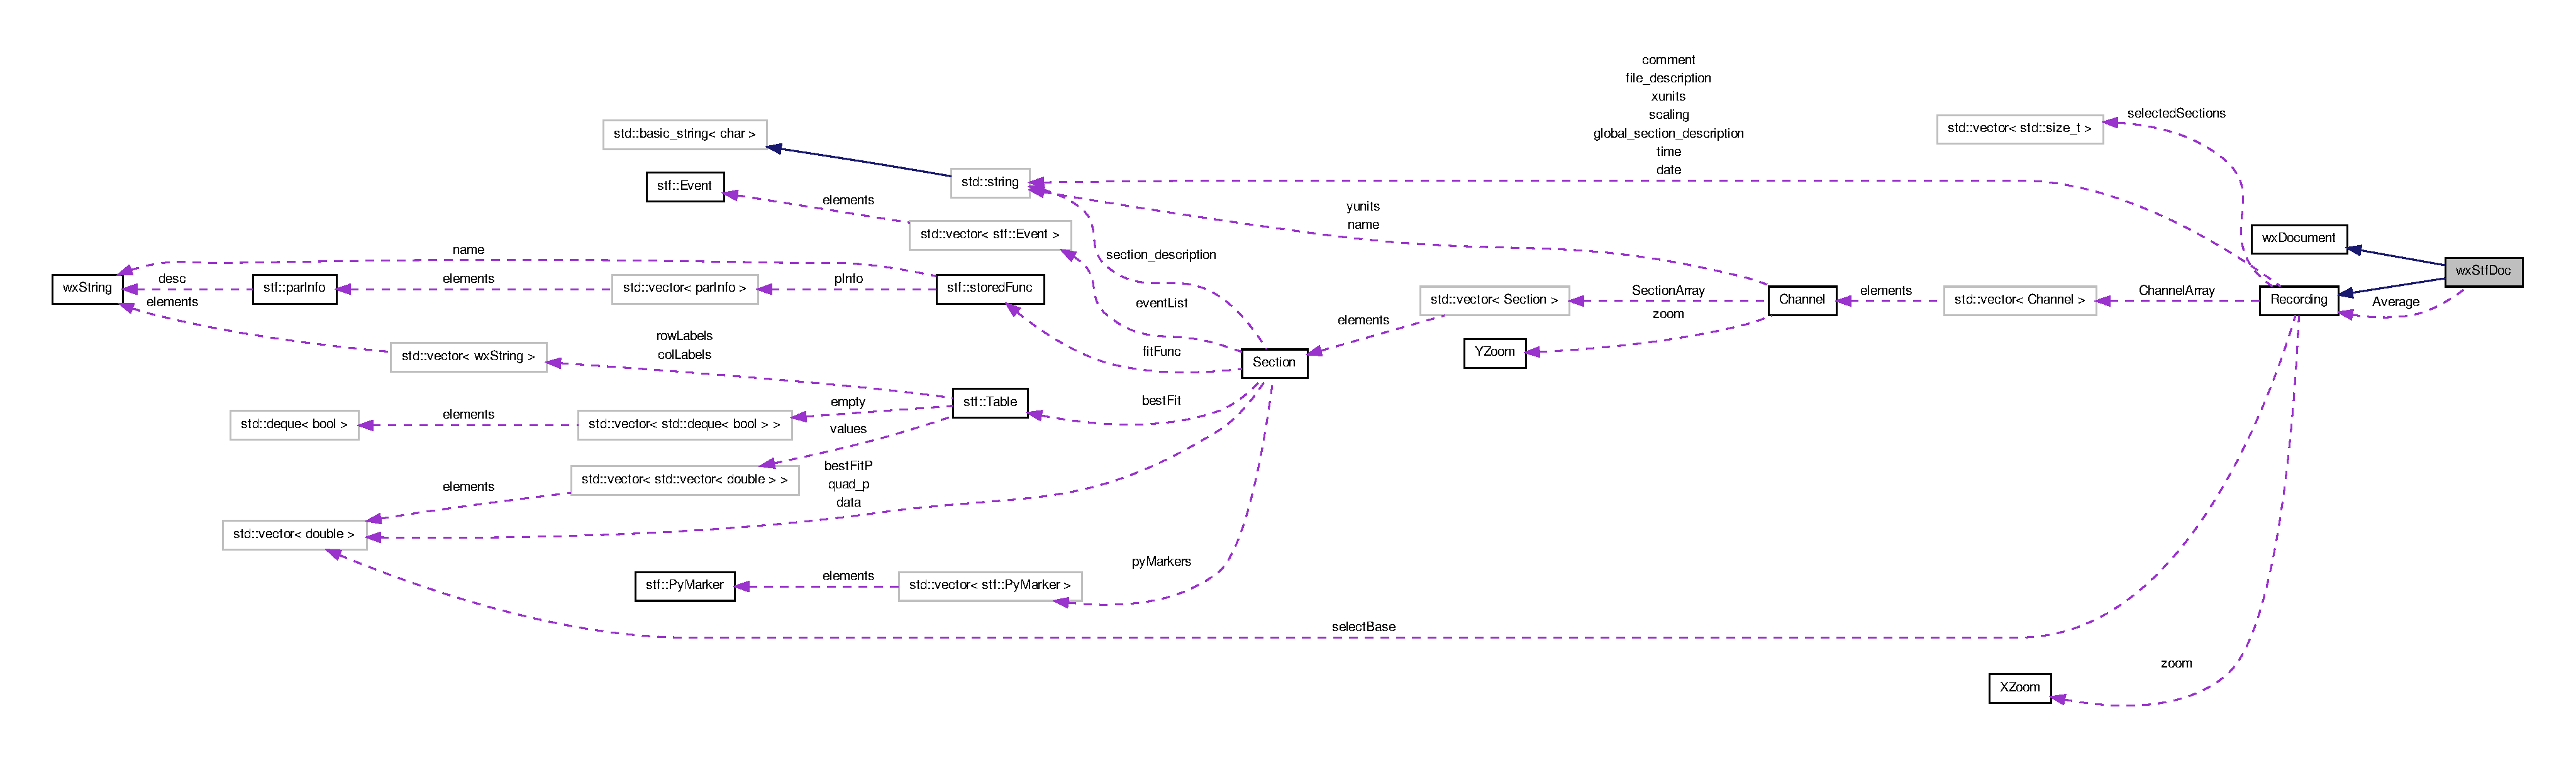
\includegraphics[width=400pt]{classwxStfDoc__coll__graph}
\end{center}
\end{figure}
\subsection*{Public Member Functions}
\begin{DoxyCompactItemize}
\item 
\hyperlink{classwxStfDoc_ad4ee4f13f7122ae8127b12056f4c5c49}{wxStfDoc} ()
\begin{DoxyCompactList}\small\item\em Constructor. \item\end{DoxyCompactList}\item 
\hypertarget{classwxStfDoc_af08b1b2f973cc9ff74bdce3b645b07f0}{
\hyperlink{classwxStfDoc_af08b1b2f973cc9ff74bdce3b645b07f0}{$\sim$wxStfDoc} ()}
\label{classwxStfDoc_af08b1b2f973cc9ff74bdce3b645b07f0}

\begin{DoxyCompactList}\small\item\em Destructor. \item\end{DoxyCompactList}\item 
virtual bool \hyperlink{classwxStfDoc_aa0d559931da793946eec24221ca53f1b}{OnOpenDocument} (const \hyperlink{classwxString}{wxString} \&filename)
\begin{DoxyCompactList}\small\item\em Override default file opening. \item\end{DoxyCompactList}\item 
virtual bool \hyperlink{classwxStfDoc_a02d5b6f21c9ac17f7fc6c43f7f8220d2}{OnOpenPyDocument} (const \hyperlink{classwxString}{wxString} \&filename)
\begin{DoxyCompactList}\small\item\em Open document without progress dialog. \item\end{DoxyCompactList}\item 
virtual bool \hyperlink{classwxStfDoc_a3aea82075c22916ae4ac88016b52cb19}{SaveAs} ()
\begin{DoxyCompactList}\small\item\em Override default file saving. \item\end{DoxyCompactList}\item 
virtual bool \hyperlink{classwxStfDoc_a7ad8f08b21de30f6031d16eecfb965ef}{DoSaveDocument} (const \hyperlink{classwxString}{wxString} \&filename)
\begin{DoxyCompactList}\small\item\em Override default file saving. \item\end{DoxyCompactList}\item 
virtual bool \hyperlink{classwxStfDoc_aeb6ac6149de1d6f580bde0d220810d2d}{OnCloseDocument} ()
\begin{DoxyCompactList}\small\item\em Override default file closing. \item\end{DoxyCompactList}\item 
virtual bool \hyperlink{classwxStfDoc_a1ec2a08fd79dfa8424ac0c48571ed6c9}{OnNewDocument} ()
\begin{DoxyCompactList}\small\item\em Override default file creation. \item\end{DoxyCompactList}\item 
void \hyperlink{classwxStfDoc_a6e9f245187dc5656b655b205aaa35b56}{SetData} (const \hyperlink{classRecording}{Recording} \&c\_\-Data, const \hyperlink{classwxStfDoc}{wxStfDoc} $\ast$Sender, const \hyperlink{classwxString}{wxString} \&title)
\begin{DoxyCompactList}\small\item\em Sets the content of a newly created file. \item\end{DoxyCompactList}\item 
bool \hyperlink{classwxStfDoc_a4e71318907a99c8a05aa9fd05e660aa8}{GetIsAverage} () const 
\begin{DoxyCompactList}\small\item\em Indicates whether an average has been created. \item\end{DoxyCompactList}\item 
bool \hyperlink{classwxStfDoc_a9a1a53d398d157a6fbc3c76a1046f915}{GetPeakAtEnd} () const 
\begin{DoxyCompactList}\small\item\em Indicates whether the right peak cursor should always be at the end of a trace. \item\end{DoxyCompactList}\item 
bool \hyperlink{classwxStfDoc_a75a4270ebe16b66e2a171260b94f6ba3}{IsInitialized} () const 
\begin{DoxyCompactList}\small\item\em Indicates whether the the document is fully initialised. \item\end{DoxyCompactList}\item 
void \hyperlink{classwxStfDoc_acebb27e8f79da6253877bb7e0058273e}{SetPeakAtEnd} (bool value)
\begin{DoxyCompactList}\small\item\em Sets the right peak cursor to the end of a trace. \item\end{DoxyCompactList}\item 
const \hyperlink{classRecording}{Recording} \& \hyperlink{classwxStfDoc_aba369f7488cd4b4552e4a237d84d9f1c}{GetAverage} () const 
\begin{DoxyCompactList}\small\item\em Retrieves the average trace(s). \item\end{DoxyCompactList}\item 
\hypertarget{classwxStfDoc_a03dc14c52d0e354f1b2366d7869caf54}{
void \hyperlink{classwxStfDoc_a03dc14c52d0e354f1b2366d7869caf54}{CheckBoundaries} ()}
\label{classwxStfDoc_a03dc14c52d0e354f1b2366d7869caf54}

\begin{DoxyCompactList}\small\item\em Checks whether any cursor is reversed or out of range and corrects it if required. \item\end{DoxyCompactList}\item 
\hypertarget{classwxStfDoc_aa2ec0e9a57dfa2d3d0debb8045eb6d4c}{
void \hyperlink{classwxStfDoc_aa2ec0e9a57dfa2d3d0debb8045eb6d4c}{UpdateMenuCheckmarks} ()}
\label{classwxStfDoc_aa2ec0e9a57dfa2d3d0debb8045eb6d4c}

\begin{DoxyCompactList}\small\item\em Updates the check marks in the latency mode menu. \item\end{DoxyCompactList}\item 
bool \hyperlink{classwxStfDoc_ab4a211cde4a5861c29fbdb550598abb5}{SetSection} (std::size\_\-t section)
\begin{DoxyCompactList}\small\item\em Sets the current section to the specified value. \item\end{DoxyCompactList}\item 
bool \hyperlink{classwxStfDoc_a3ef8caec9a376d179e6eadae7ff25aa3}{OnNewfromselectedThis} ()
\begin{DoxyCompactList}\small\item\em Creates a new window containing the selected sections of this file. \item\end{DoxyCompactList}\item 
void \hyperlink{classwxStfDoc_a42949b9f9cbc3f4859df05c900f74a68}{Selectall} (\hyperlink{classwxCommandEvent}{wxCommandEvent} \&event)
\begin{DoxyCompactList}\small\item\em Selects all sections. \item\end{DoxyCompactList}\item 
void \hyperlink{classwxStfDoc_ae5d2d78952dab927680a42588a75418f}{Deleteselected} (\hyperlink{classwxCommandEvent}{wxCommandEvent} \&event)
\begin{DoxyCompactList}\small\item\em Unselects all sections. \item\end{DoxyCompactList}\item 
\hypertarget{classwxStfDoc_ab1fb4e6a7c9e727e2f6051552e595c8c}{
void \hyperlink{classwxStfDoc_ab1fb4e6a7c9e727e2f6051552e595c8c}{UpdateSelectedButton} ()}
\label{classwxStfDoc_ab1fb4e6a7c9e727e2f6051552e595c8c}

\begin{DoxyCompactList}\small\item\em Updates the status of the selection button. \item\end{DoxyCompactList}\item 
void \hyperlink{classwxStfDoc_af955698664d1db45669e2be7b7c5d1dc}{CreateAverage} (bool calcSD, bool align)
\begin{DoxyCompactList}\small\item\em Creates an average trace from the selected sections. \item\end{DoxyCompactList}\item 
\hypertarget{classwxStfDoc_afa3040015e9534a75d28693f847507b2}{
void \hyperlink{classwxStfDoc_afa3040015e9534a75d28693f847507b2}{ToggleSelect} ()}
\label{classwxStfDoc_afa3040015e9534a75d28693f847507b2}

\begin{DoxyCompactList}\small\item\em Toggles the selection status of the current section. \item\end{DoxyCompactList}\item 
\hypertarget{classwxStfDoc_a3c2dd72fbf49698c82bd89de63ea580b}{
void \hyperlink{classwxStfDoc_a3c2dd72fbf49698c82bd89de63ea580b}{Select} ()}
\label{classwxStfDoc_a3c2dd72fbf49698c82bd89de63ea580b}

\begin{DoxyCompactList}\small\item\em Selects the current section if previously unselected. \item\end{DoxyCompactList}\item 
\hypertarget{classwxStfDoc_aba7a580a21ff332dd87b43ddc383c0fe}{
void \hyperlink{classwxStfDoc_aba7a580a21ff332dd87b43ddc383c0fe}{Remove} ()}
\label{classwxStfDoc_aba7a580a21ff332dd87b43ddc383c0fe}

\begin{DoxyCompactList}\small\item\em Unselects the current section if previously selected. \item\end{DoxyCompactList}\item 
void \hyperlink{classwxStfDoc_ad46aafbc7c933ae72da528915a43f449}{Extract} (\hyperlink{classwxCommandEvent}{wxCommandEvent} \&event)
\begin{DoxyCompactList}\small\item\em Creates a new document from the checked events. \item\end{DoxyCompactList}\item 
void \hyperlink{classwxStfDoc_ae97d84b92aaf67309f514d1e8e9c739c}{EraseEvents} (\hyperlink{classwxCommandEvent}{wxCommandEvent} \&event)
\begin{DoxyCompactList}\small\item\em Erases all events, independent of whether they are checked or not. \item\end{DoxyCompactList}\item 
void \hyperlink{classwxStfDoc_a8be8771a4348f17969b786fa88884723}{AddEvent} (\hyperlink{classwxCommandEvent}{wxCommandEvent} \&event)
\begin{DoxyCompactList}\small\item\em Adds an event at the current eventPos. \item\end{DoxyCompactList}\item 
bool \hyperlink{classwxStfDoc_a3c758286d53c9d2a2f4db8eb11128cc7}{SubtractBase} ()
\begin{DoxyCompactList}\small\item\em Subtracts the baseline of all selected traces. \item\end{DoxyCompactList}\item 
void \hyperlink{classwxStfDoc_a0e36306341c1684f9691a05cbd2b8825}{FitDecay} (\hyperlink{classwxCommandEvent}{wxCommandEvent} \&event)
\begin{DoxyCompactList}\small\item\em Fit a function to the data. \item\end{DoxyCompactList}\item 
void \hyperlink{classwxStfDoc_a98616f1e6ced3992ba32a9080c86060a}{SetFileMenu} (wxMenu $\ast$menu)
\begin{DoxyCompactList}\small\item\em Sets a pointer to the file menu attached to this document. \item\end{DoxyCompactList}\end{DoxyCompactItemize}


\subsection{Detailed Description}
The document class, derived from both \hyperlink{classwxDocument}{wxDocument} and \hyperlink{classRecording}{Recording}. The document class can be used to model an application’s file-\/based data. It is part of the document/view framework supported by wxWidgets. 

\subsection{Constructor \& Destructor Documentation}
\hypertarget{classwxStfDoc_ad4ee4f13f7122ae8127b12056f4c5c49}{
\index{wxStfDoc@{wxStfDoc}!wxStfDoc@{wxStfDoc}}
\index{wxStfDoc@{wxStfDoc}!wxStfDoc@{wxStfDoc}}
\subsubsection[{wxStfDoc}]{\setlength{\rightskip}{0pt plus 5cm}wxStfDoc::wxStfDoc (
\begin{DoxyParamCaption}
{}
\end{DoxyParamCaption}
)}}
\label{classwxStfDoc_ad4ee4f13f7122ae8127b12056f4c5c49}


Constructor. 

Does nothing but initialising the member list. 

\subsection{Member Function Documentation}
\hypertarget{classwxStfDoc_a8be8771a4348f17969b786fa88884723}{
\index{wxStfDoc@{wxStfDoc}!AddEvent@{AddEvent}}
\index{AddEvent@{AddEvent}!wxStfDoc@{wxStfDoc}}
\subsubsection[{AddEvent}]{\setlength{\rightskip}{0pt plus 5cm}void wxStfDoc::AddEvent (
\begin{DoxyParamCaption}
\item[{{\bf wxCommandEvent} \&}]{event}
\end{DoxyParamCaption}
)}}
\label{classwxStfDoc_a8be8771a4348f17969b786fa88884723}


Adds an event at the current eventPos. 


\begin{DoxyParams}{Parameters}
{\em event} & The menu event that made the call. \\
\hline
\end{DoxyParams}
\hypertarget{classwxStfDoc_af955698664d1db45669e2be7b7c5d1dc}{
\index{wxStfDoc@{wxStfDoc}!CreateAverage@{CreateAverage}}
\index{CreateAverage@{CreateAverage}!wxStfDoc@{wxStfDoc}}
\subsubsection[{CreateAverage}]{\setlength{\rightskip}{0pt plus 5cm}void wxStfDoc::CreateAverage (
\begin{DoxyParamCaption}
\item[{bool}]{calcSD, }
\item[{bool}]{align}
\end{DoxyParamCaption}
)}}
\label{classwxStfDoc_af955698664d1db45669e2be7b7c5d1dc}


Creates an average trace from the selected sections. 


\begin{DoxyParams}{Parameters}
{\em calcSD} & Set to true if the standard deviation should be calculated as well, false otherwise \\
\hline
{\em align} & Set to true if traces should be aligned to the point of steepest rise of the inactive channel, false otherwise. \\
\hline
\end{DoxyParams}
\hypertarget{classwxStfDoc_ae5d2d78952dab927680a42588a75418f}{
\index{wxStfDoc@{wxStfDoc}!Deleteselected@{Deleteselected}}
\index{Deleteselected@{Deleteselected}!wxStfDoc@{wxStfDoc}}
\subsubsection[{Deleteselected}]{\setlength{\rightskip}{0pt plus 5cm}void wxStfDoc::Deleteselected (
\begin{DoxyParamCaption}
\item[{{\bf wxCommandEvent} \&}]{event}
\end{DoxyParamCaption}
)}}
\label{classwxStfDoc_ae5d2d78952dab927680a42588a75418f}


Unselects all sections. 


\begin{DoxyParams}{Parameters}
{\em event} & The menu event that made the call. \\
\hline
\end{DoxyParams}
\hypertarget{classwxStfDoc_a7ad8f08b21de30f6031d16eecfb965ef}{
\index{wxStfDoc@{wxStfDoc}!DoSaveDocument@{DoSaveDocument}}
\index{DoSaveDocument@{DoSaveDocument}!wxStfDoc@{wxStfDoc}}
\subsubsection[{DoSaveDocument}]{\setlength{\rightskip}{0pt plus 5cm}virtual bool wxStfDoc::DoSaveDocument (
\begin{DoxyParamCaption}
\item[{const {\bf wxString} \&}]{filename}
\end{DoxyParamCaption}
)\hspace{0.3cm}{\ttfamily  \mbox{[}virtual\mbox{]}}}}
\label{classwxStfDoc_a7ad8f08b21de30f6031d16eecfb965ef}


Override default file saving. 


\begin{DoxyParams}{Parameters}
{\em filename} & Full path of the file. \\
\hline
\end{DoxyParams}
\begin{DoxyReturn}{Returns}
true if successfully saved, false otherwise. 
\end{DoxyReturn}
\hypertarget{classwxStfDoc_ae97d84b92aaf67309f514d1e8e9c739c}{
\index{wxStfDoc@{wxStfDoc}!EraseEvents@{EraseEvents}}
\index{EraseEvents@{EraseEvents}!wxStfDoc@{wxStfDoc}}
\subsubsection[{EraseEvents}]{\setlength{\rightskip}{0pt plus 5cm}void wxStfDoc::EraseEvents (
\begin{DoxyParamCaption}
\item[{{\bf wxCommandEvent} \&}]{event}
\end{DoxyParamCaption}
)}}
\label{classwxStfDoc_ae97d84b92aaf67309f514d1e8e9c739c}


Erases all events, independent of whether they are checked or not. 


\begin{DoxyParams}{Parameters}
{\em event} & The menu event that made the call. \\
\hline
\end{DoxyParams}
\hypertarget{classwxStfDoc_ad46aafbc7c933ae72da528915a43f449}{
\index{wxStfDoc@{wxStfDoc}!Extract@{Extract}}
\index{Extract@{Extract}!wxStfDoc@{wxStfDoc}}
\subsubsection[{Extract}]{\setlength{\rightskip}{0pt plus 5cm}void wxStfDoc::Extract (
\begin{DoxyParamCaption}
\item[{{\bf wxCommandEvent} \&}]{event}
\end{DoxyParamCaption}
)}}
\label{classwxStfDoc_ad46aafbc7c933ae72da528915a43f449}


Creates a new document from the checked events. 


\begin{DoxyParams}{Parameters}
{\em event} & The menu event that made the call. \\
\hline
\end{DoxyParams}
\hypertarget{classwxStfDoc_a0e36306341c1684f9691a05cbd2b8825}{
\index{wxStfDoc@{wxStfDoc}!FitDecay@{FitDecay}}
\index{FitDecay@{FitDecay}!wxStfDoc@{wxStfDoc}}
\subsubsection[{FitDecay}]{\setlength{\rightskip}{0pt plus 5cm}void wxStfDoc::FitDecay (
\begin{DoxyParamCaption}
\item[{{\bf wxCommandEvent} \&}]{event}
\end{DoxyParamCaption}
)}}
\label{classwxStfDoc_a0e36306341c1684f9691a05cbd2b8825}


Fit a function to the data. 


\begin{DoxyParams}{Parameters}
{\em event} & The menu event that made the call. \\
\hline
\end{DoxyParams}
\hypertarget{classwxStfDoc_aba369f7488cd4b4552e4a237d84d9f1c}{
\index{wxStfDoc@{wxStfDoc}!GetAverage@{GetAverage}}
\index{GetAverage@{GetAverage}!wxStfDoc@{wxStfDoc}}
\subsubsection[{GetAverage}]{\setlength{\rightskip}{0pt plus 5cm}const {\bf Recording}\& wxStfDoc::GetAverage (
\begin{DoxyParamCaption}
{}
\end{DoxyParamCaption}
) const\hspace{0.3cm}{\ttfamily  \mbox{[}inline\mbox{]}}}}
\label{classwxStfDoc_aba369f7488cd4b4552e4a237d84d9f1c}


Retrieves the average trace(s). 

\begin{DoxyReturn}{Returns}
The average trace as a \hyperlink{classRecording}{Recording} object. 
\end{DoxyReturn}
\hypertarget{classwxStfDoc_a4e71318907a99c8a05aa9fd05e660aa8}{
\index{wxStfDoc@{wxStfDoc}!GetIsAverage@{GetIsAverage}}
\index{GetIsAverage@{GetIsAverage}!wxStfDoc@{wxStfDoc}}
\subsubsection[{GetIsAverage}]{\setlength{\rightskip}{0pt plus 5cm}bool wxStfDoc::GetIsAverage (
\begin{DoxyParamCaption}
{}
\end{DoxyParamCaption}
) const\hspace{0.3cm}{\ttfamily  \mbox{[}inline\mbox{]}}}}
\label{classwxStfDoc_a4e71318907a99c8a05aa9fd05e660aa8}


Indicates whether an average has been created. 

\begin{DoxyReturn}{Returns}
true if an average has been created, false otherwise. 
\end{DoxyReturn}
\hypertarget{classwxStfDoc_a9a1a53d398d157a6fbc3c76a1046f915}{
\index{wxStfDoc@{wxStfDoc}!GetPeakAtEnd@{GetPeakAtEnd}}
\index{GetPeakAtEnd@{GetPeakAtEnd}!wxStfDoc@{wxStfDoc}}
\subsubsection[{GetPeakAtEnd}]{\setlength{\rightskip}{0pt plus 5cm}bool wxStfDoc::GetPeakAtEnd (
\begin{DoxyParamCaption}
{}
\end{DoxyParamCaption}
) const\hspace{0.3cm}{\ttfamily  \mbox{[}inline\mbox{]}}}}
\label{classwxStfDoc_a9a1a53d398d157a6fbc3c76a1046f915}


Indicates whether the right peak cursor should always be at the end of a trace. 

\begin{DoxyReturn}{Returns}
true if the right peak cursor should be at the end, false otherwise. 
\end{DoxyReturn}
\hypertarget{classwxStfDoc_a75a4270ebe16b66e2a171260b94f6ba3}{
\index{wxStfDoc@{wxStfDoc}!IsInitialized@{IsInitialized}}
\index{IsInitialized@{IsInitialized}!wxStfDoc@{wxStfDoc}}
\subsubsection[{IsInitialized}]{\setlength{\rightskip}{0pt plus 5cm}bool wxStfDoc::IsInitialized (
\begin{DoxyParamCaption}
{}
\end{DoxyParamCaption}
) const\hspace{0.3cm}{\ttfamily  \mbox{[}inline\mbox{]}}}}
\label{classwxStfDoc_a75a4270ebe16b66e2a171260b94f6ba3}


Indicates whether the the document is fully initialised. 

The document has to be fully initialized before other parts of the program start accessing it; for example, the graph might start reading out values before they exist. \begin{DoxyReturn}{Returns}
true if the document is fully initialised, false otherwise. 
\end{DoxyReturn}
\hypertarget{classwxStfDoc_aeb6ac6149de1d6f580bde0d220810d2d}{
\index{wxStfDoc@{wxStfDoc}!OnCloseDocument@{OnCloseDocument}}
\index{OnCloseDocument@{OnCloseDocument}!wxStfDoc@{wxStfDoc}}
\subsubsection[{OnCloseDocument}]{\setlength{\rightskip}{0pt plus 5cm}virtual bool wxStfDoc::OnCloseDocument (
\begin{DoxyParamCaption}
{}
\end{DoxyParamCaption}
)\hspace{0.3cm}{\ttfamily  \mbox{[}virtual\mbox{]}}}}
\label{classwxStfDoc_aeb6ac6149de1d6f580bde0d220810d2d}


Override default file closing. 

Writes settings to the config file or registry before closing. \begin{DoxyReturn}{Returns}
true if successfully closed, false otherwise. 
\end{DoxyReturn}
\hypertarget{classwxStfDoc_a1ec2a08fd79dfa8424ac0c48571ed6c9}{
\index{wxStfDoc@{wxStfDoc}!OnNewDocument@{OnNewDocument}}
\index{OnNewDocument@{OnNewDocument}!wxStfDoc@{wxStfDoc}}
\subsubsection[{OnNewDocument}]{\setlength{\rightskip}{0pt plus 5cm}virtual bool wxStfDoc::OnNewDocument (
\begin{DoxyParamCaption}
{}
\end{DoxyParamCaption}
)\hspace{0.3cm}{\ttfamily  \mbox{[}virtual\mbox{]}}}}
\label{classwxStfDoc_a1ec2a08fd79dfa8424ac0c48571ed6c9}


Override default file creation. 

\begin{DoxyReturn}{Returns}
true if successfully closed, false otherwise. 
\end{DoxyReturn}
\hypertarget{classwxStfDoc_a3ef8caec9a376d179e6eadae7ff25aa3}{
\index{wxStfDoc@{wxStfDoc}!OnNewfromselectedThis@{OnNewfromselectedThis}}
\index{OnNewfromselectedThis@{OnNewfromselectedThis}!wxStfDoc@{wxStfDoc}}
\subsubsection[{OnNewfromselectedThis}]{\setlength{\rightskip}{0pt plus 5cm}bool wxStfDoc::OnNewfromselectedThis (
\begin{DoxyParamCaption}
{}
\end{DoxyParamCaption}
)}}
\label{classwxStfDoc_a3ef8caec9a376d179e6eadae7ff25aa3}


Creates a new window containing the selected sections of this file. 

\begin{DoxyReturn}{Returns}
true upon success, false otherwise. 
\end{DoxyReturn}
\hypertarget{classwxStfDoc_aa0d559931da793946eec24221ca53f1b}{
\index{wxStfDoc@{wxStfDoc}!OnOpenDocument@{OnOpenDocument}}
\index{OnOpenDocument@{OnOpenDocument}!wxStfDoc@{wxStfDoc}}
\subsubsection[{OnOpenDocument}]{\setlength{\rightskip}{0pt plus 5cm}virtual bool wxStfDoc::OnOpenDocument (
\begin{DoxyParamCaption}
\item[{const {\bf wxString} \&}]{filename}
\end{DoxyParamCaption}
)\hspace{0.3cm}{\ttfamily  \mbox{[}virtual\mbox{]}}}}
\label{classwxStfDoc_aa0d559931da793946eec24221ca53f1b}


Override default file opening. 

Attempts to identify the file type from the filter extension (such as \char`\"{}$\ast$.dat\char`\"{}) 
\begin{DoxyParams}{Parameters}
{\em filename} & Full path of the file. \\
\hline
\end{DoxyParams}
\begin{DoxyReturn}{Returns}
true if successfully opened, false otherwise. 
\end{DoxyReturn}
\hypertarget{classwxStfDoc_a02d5b6f21c9ac17f7fc6c43f7f8220d2}{
\index{wxStfDoc@{wxStfDoc}!OnOpenPyDocument@{OnOpenPyDocument}}
\index{OnOpenPyDocument@{OnOpenPyDocument}!wxStfDoc@{wxStfDoc}}
\subsubsection[{OnOpenPyDocument}]{\setlength{\rightskip}{0pt plus 5cm}virtual bool wxStfDoc::OnOpenPyDocument (
\begin{DoxyParamCaption}
\item[{const {\bf wxString} \&}]{filename}
\end{DoxyParamCaption}
)\hspace{0.3cm}{\ttfamily  \mbox{[}virtual\mbox{]}}}}
\label{classwxStfDoc_a02d5b6f21c9ac17f7fc6c43f7f8220d2}


Open document without progress dialog. 

Attempts to identify the file type from the filter extension (such as \char`\"{}$\ast$.dat\char`\"{}) 
\begin{DoxyParams}{Parameters}
{\em filename} & Full path of the file. \\
\hline
\end{DoxyParams}
\begin{DoxyReturn}{Returns}
true if successfully opened, false otherwise. 
\end{DoxyReturn}
\hypertarget{classwxStfDoc_a3aea82075c22916ae4ac88016b52cb19}{
\index{wxStfDoc@{wxStfDoc}!SaveAs@{SaveAs}}
\index{SaveAs@{SaveAs}!wxStfDoc@{wxStfDoc}}
\subsubsection[{SaveAs}]{\setlength{\rightskip}{0pt plus 5cm}virtual bool wxStfDoc::SaveAs (
\begin{DoxyParamCaption}
{}
\end{DoxyParamCaption}
)\hspace{0.3cm}{\ttfamily  \mbox{[}virtual\mbox{]}}}}
\label{classwxStfDoc_a3aea82075c22916ae4ac88016b52cb19}


Override default file saving. 

\begin{DoxyReturn}{Returns}
true if successfully saved, false otherwise. 
\end{DoxyReturn}
\hypertarget{classwxStfDoc_a42949b9f9cbc3f4859df05c900f74a68}{
\index{wxStfDoc@{wxStfDoc}!Selectall@{Selectall}}
\index{Selectall@{Selectall}!wxStfDoc@{wxStfDoc}}
\subsubsection[{Selectall}]{\setlength{\rightskip}{0pt plus 5cm}void wxStfDoc::Selectall (
\begin{DoxyParamCaption}
\item[{{\bf wxCommandEvent} \&}]{event}
\end{DoxyParamCaption}
)}}
\label{classwxStfDoc_a42949b9f9cbc3f4859df05c900f74a68}


Selects all sections. 


\begin{DoxyParams}{Parameters}
{\em event} & The menu event that made the call. \\
\hline
\end{DoxyParams}
\hypertarget{classwxStfDoc_a6e9f245187dc5656b655b205aaa35b56}{
\index{wxStfDoc@{wxStfDoc}!SetData@{SetData}}
\index{SetData@{SetData}!wxStfDoc@{wxStfDoc}}
\subsubsection[{SetData}]{\setlength{\rightskip}{0pt plus 5cm}void wxStfDoc::SetData (
\begin{DoxyParamCaption}
\item[{const {\bf Recording} \&}]{c\_\-Data, }
\item[{const {\bf wxStfDoc} $\ast$}]{Sender, }
\item[{const {\bf wxString} \&}]{title}
\end{DoxyParamCaption}
)}}
\label{classwxStfDoc_a6e9f245187dc5656b655b205aaa35b56}


Sets the content of a newly created file. 


\begin{DoxyParams}{Parameters}
{\em c\_\-Data} & The data that is used for the new file. \\
\hline
{\em Sender} & Pointer to the document that generated this file. \\
\hline
{\em title} & Title of the new document. \\
\hline
\end{DoxyParams}
\hypertarget{classwxStfDoc_a98616f1e6ced3992ba32a9080c86060a}{
\index{wxStfDoc@{wxStfDoc}!SetFileMenu@{SetFileMenu}}
\index{SetFileMenu@{SetFileMenu}!wxStfDoc@{wxStfDoc}}
\subsubsection[{SetFileMenu}]{\setlength{\rightskip}{0pt plus 5cm}void wxStfDoc::SetFileMenu (
\begin{DoxyParamCaption}
\item[{wxMenu $\ast$}]{menu}
\end{DoxyParamCaption}
)\hspace{0.3cm}{\ttfamily  \mbox{[}inline\mbox{]}}}}
\label{classwxStfDoc_a98616f1e6ced3992ba32a9080c86060a}


Sets a pointer to the file menu attached to this document. 


\begin{DoxyParams}{Parameters}
{\em menu} & The menu to be attached. \\
\hline
\end{DoxyParams}
\hypertarget{classwxStfDoc_acebb27e8f79da6253877bb7e0058273e}{
\index{wxStfDoc@{wxStfDoc}!SetPeakAtEnd@{SetPeakAtEnd}}
\index{SetPeakAtEnd@{SetPeakAtEnd}!wxStfDoc@{wxStfDoc}}
\subsubsection[{SetPeakAtEnd}]{\setlength{\rightskip}{0pt plus 5cm}void wxStfDoc::SetPeakAtEnd (
\begin{DoxyParamCaption}
\item[{bool}]{value}
\end{DoxyParamCaption}
)\hspace{0.3cm}{\ttfamily  \mbox{[}inline\mbox{]}}}}
\label{classwxStfDoc_acebb27e8f79da6253877bb7e0058273e}


Sets the right peak cursor to the end of a trace. 


\begin{DoxyParams}{Parameters}
{\em value} & determines whether the peak cursor should be at the end of a trace. \\
\hline
\end{DoxyParams}
\hypertarget{classwxStfDoc_ab4a211cde4a5861c29fbdb550598abb5}{
\index{wxStfDoc@{wxStfDoc}!SetSection@{SetSection}}
\index{SetSection@{SetSection}!wxStfDoc@{wxStfDoc}}
\subsubsection[{SetSection}]{\setlength{\rightskip}{0pt plus 5cm}bool wxStfDoc::SetSection (
\begin{DoxyParamCaption}
\item[{std::size\_\-t}]{section}
\end{DoxyParamCaption}
)}}
\label{classwxStfDoc_ab4a211cde4a5861c29fbdb550598abb5}


Sets the current section to the specified value. 

Checks for out-\/of-\/range errors 
\begin{DoxyParams}{Parameters}
{\em section} & The 0-\/based index of the new section \\
\hline
\end{DoxyParams}
\hypertarget{classwxStfDoc_a3c758286d53c9d2a2f4db8eb11128cc7}{
\index{wxStfDoc@{wxStfDoc}!SubtractBase@{SubtractBase}}
\index{SubtractBase@{SubtractBase}!wxStfDoc@{wxStfDoc}}
\subsubsection[{SubtractBase}]{\setlength{\rightskip}{0pt plus 5cm}bool wxStfDoc::SubtractBase (
\begin{DoxyParamCaption}
{}
\end{DoxyParamCaption}
)}}
\label{classwxStfDoc_a3c758286d53c9d2a2f4db8eb11128cc7}


Subtracts the baseline of all selected traces. 

\begin{DoxyReturn}{Returns}
true upon success, false otherwise. 
\end{DoxyReturn}


The documentation for this class was generated from the following file:\begin{DoxyCompactItemize}
\item 
src/app/\hyperlink{doc_8h}{doc.h}\end{DoxyCompactItemize}

\hypertarget{classwxStfEventDlg}{
\section{wxStfEventDlg Class Reference}
\label{classwxStfEventDlg}\index{wxStfEventDlg@{wxStfEventDlg}}
}


Dialog for event-\/detection settings.  




{\ttfamily \#include $<$eventdlg.h$>$}



Inheritance diagram for wxStfEventDlg:
\nopagebreak
\begin{figure}[H]
\begin{center}
\leavevmode
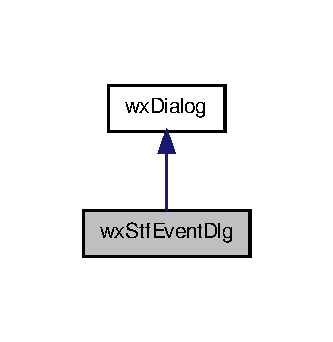
\includegraphics[width=160pt]{classwxStfEventDlg__inherit__graph}
\end{center}
\end{figure}


Collaboration diagram for wxStfEventDlg:
\nopagebreak
\begin{figure}[H]
\begin{center}
\leavevmode
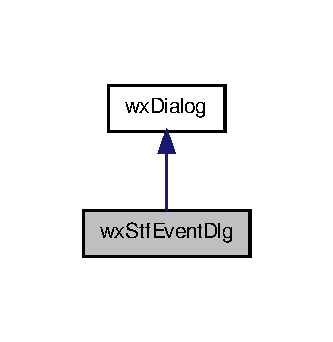
\includegraphics[width=160pt]{classwxStfEventDlg__coll__graph}
\end{center}
\end{figure}
\subsection*{Public Member Functions}
\begin{DoxyCompactItemize}
\item 
\hyperlink{classwxStfEventDlg_a9a2b621347c3b7023925bf34fbc6aec8}{wxStfEventDlg} (\hyperlink{classwxWindow}{wxWindow} $\ast$parent, const std::vector$<$ \hyperlink{classSection}{Section} $\ast$ $>$ \&templateSections, bool isExtract, int id=wxID\_\-ANY, \hyperlink{classwxString}{wxString} title=wxT(\char`\"{}Event detection settings\char`\"{}), wxPoint pos=wxDefaultPosition, \hyperlink{classwxSize}{wxSize} size=wxDefaultSize, int style=wxCAPTION)
\begin{DoxyCompactList}\small\item\em Constructor. \item\end{DoxyCompactList}\item 
double \hyperlink{classwxStfEventDlg_a9d8b27333f9876691d79d0e30a1458ee}{GetThreshold} () const 
\begin{DoxyCompactList}\small\item\em Get the event detection threshold. \item\end{DoxyCompactList}\item 
bool \hyperlink{classwxStfEventDlg_a42308a83a05ad311035411807618cdcf}{GetScaling} () const 
\begin{DoxyCompactList}\small\item\em Indicates whether template scaling or the correlation coefficient should be used. \item\end{DoxyCompactList}\item 
int \hyperlink{classwxStfEventDlg_a8c1e61f0d00bebd250cc84995994f3e4}{GetMinDistance} () const 
\begin{DoxyCompactList}\small\item\em Get the minimal distance between events. \item\end{DoxyCompactList}\item 
int \hyperlink{classwxStfEventDlg_a93043c17a21791ecc9d59d28d06f76f6}{GetTemplate} () const 
\begin{DoxyCompactList}\small\item\em Get the selected template. \item\end{DoxyCompactList}\item 
virtual void \hyperlink{classwxStfEventDlg_a986b0e424be3432d17c20e7507e03519}{EndModal} (int retCode)
\begin{DoxyCompactList}\small\item\em Called upon ending a modal dialog. \item\end{DoxyCompactList}\end{DoxyCompactItemize}


\subsection{Detailed Description}
Dialog for event-\/detection settings. 

\subsection{Constructor \& Destructor Documentation}
\hypertarget{classwxStfEventDlg_a9a2b621347c3b7023925bf34fbc6aec8}{
\index{wxStfEventDlg@{wxStfEventDlg}!wxStfEventDlg@{wxStfEventDlg}}
\index{wxStfEventDlg@{wxStfEventDlg}!wxStfEventDlg@{wxStfEventDlg}}
\subsubsection[{wxStfEventDlg}]{\setlength{\rightskip}{0pt plus 5cm}wxStfEventDlg::wxStfEventDlg (
\begin{DoxyParamCaption}
\item[{{\bf wxWindow} $\ast$}]{parent, }
\item[{const std::vector$<$ {\bf Section} $\ast$ $>$ \&}]{templateSections, }
\item[{bool}]{isExtract, }
\item[{int}]{id = {\ttfamily wxID\_\-ANY}, }
\item[{{\bf wxString}}]{title = {\ttfamily wxT(\char`\"{}Event~detection~settings\char`\"{})}, }
\item[{{\bf wxPoint}}]{pos = {\ttfamily wxDefaultPosition}, }
\item[{{\bf wxSize}}]{size = {\ttfamily wxDefaultSize}, }
\item[{int}]{style = {\ttfamily wxCAPTION}}
\end{DoxyParamCaption}
)}}
\label{classwxStfEventDlg_a9a2b621347c3b7023925bf34fbc6aec8}


Constructor. 


\begin{DoxyParams}{Parameters}
{\em parent} & Pointer to parent window. \\
\hline
{\em templateSections} & A vector of pointers to sections that contain fits which might be used as a template. \\
\hline
{\em isExtract} & true if events are to be detected for later extraction (rather than just plotting the detection criterion or \\
\hline
{\em id} & Window id. \\
\hline
{\em title} & Dialog title. \\
\hline
{\em pos} & Initial position. \\
\hline
{\em size} & Initial size. \\
\hline
{\em style} & Dialog style. \\
\hline
\end{DoxyParams}


\subsection{Member Function Documentation}
\hypertarget{classwxStfEventDlg_a986b0e424be3432d17c20e7507e03519}{
\index{wxStfEventDlg@{wxStfEventDlg}!EndModal@{EndModal}}
\index{EndModal@{EndModal}!wxStfEventDlg@{wxStfEventDlg}}
\subsubsection[{EndModal}]{\setlength{\rightskip}{0pt plus 5cm}virtual void wxStfEventDlg::EndModal (
\begin{DoxyParamCaption}
\item[{int}]{retCode}
\end{DoxyParamCaption}
)\hspace{0.3cm}{\ttfamily  \mbox{[}virtual\mbox{]}}}}
\label{classwxStfEventDlg_a986b0e424be3432d17c20e7507e03519}


Called upon ending a modal dialog. 


\begin{DoxyParams}{Parameters}
{\em retCode} & The dialog button id that ended the dialog (e.g. wxID\_\-OK) \\
\hline
\end{DoxyParams}
\hypertarget{classwxStfEventDlg_a8c1e61f0d00bebd250cc84995994f3e4}{
\index{wxStfEventDlg@{wxStfEventDlg}!GetMinDistance@{GetMinDistance}}
\index{GetMinDistance@{GetMinDistance}!wxStfEventDlg@{wxStfEventDlg}}
\subsubsection[{GetMinDistance}]{\setlength{\rightskip}{0pt plus 5cm}int wxStfEventDlg::GetMinDistance (
\begin{DoxyParamCaption}
{}
\end{DoxyParamCaption}
) const\hspace{0.3cm}{\ttfamily  \mbox{[}inline\mbox{]}}}}
\label{classwxStfEventDlg_a8c1e61f0d00bebd250cc84995994f3e4}


Get the minimal distance between events. 

\begin{DoxyReturn}{Returns}
The minimal distance between events in units of sampling points. 
\end{DoxyReturn}
\hypertarget{classwxStfEventDlg_a42308a83a05ad311035411807618cdcf}{
\index{wxStfEventDlg@{wxStfEventDlg}!GetScaling@{GetScaling}}
\index{GetScaling@{GetScaling}!wxStfEventDlg@{wxStfEventDlg}}
\subsubsection[{GetScaling}]{\setlength{\rightskip}{0pt plus 5cm}bool wxStfEventDlg::GetScaling (
\begin{DoxyParamCaption}
{}
\end{DoxyParamCaption}
) const\hspace{0.3cm}{\ttfamily  \mbox{[}inline\mbox{]}}}}
\label{classwxStfEventDlg_a42308a83a05ad311035411807618cdcf}


Indicates whether template scaling or the correlation coefficient should be used. 

\begin{DoxyReturn}{Returns}
true if template scaling, false if the correlation coefficient should be used. 
\end{DoxyReturn}
\hypertarget{classwxStfEventDlg_a93043c17a21791ecc9d59d28d06f76f6}{
\index{wxStfEventDlg@{wxStfEventDlg}!GetTemplate@{GetTemplate}}
\index{GetTemplate@{GetTemplate}!wxStfEventDlg@{wxStfEventDlg}}
\subsubsection[{GetTemplate}]{\setlength{\rightskip}{0pt plus 5cm}int wxStfEventDlg::GetTemplate (
\begin{DoxyParamCaption}
{}
\end{DoxyParamCaption}
) const\hspace{0.3cm}{\ttfamily  \mbox{[}inline\mbox{]}}}}
\label{classwxStfEventDlg_a93043c17a21791ecc9d59d28d06f76f6}


Get the selected template. 

\begin{DoxyReturn}{Returns}
The index of the template fit to be used for event detection. 
\end{DoxyReturn}
\hypertarget{classwxStfEventDlg_a9d8b27333f9876691d79d0e30a1458ee}{
\index{wxStfEventDlg@{wxStfEventDlg}!GetThreshold@{GetThreshold}}
\index{GetThreshold@{GetThreshold}!wxStfEventDlg@{wxStfEventDlg}}
\subsubsection[{GetThreshold}]{\setlength{\rightskip}{0pt plus 5cm}double wxStfEventDlg::GetThreshold (
\begin{DoxyParamCaption}
{}
\end{DoxyParamCaption}
) const\hspace{0.3cm}{\ttfamily  \mbox{[}inline\mbox{]}}}}
\label{classwxStfEventDlg_a9d8b27333f9876691d79d0e30a1458ee}


Get the event detection threshold. 

\begin{DoxyReturn}{Returns}
The event detection threshold. 
\end{DoxyReturn}


The documentation for this class was generated from the following file:\begin{DoxyCompactItemize}
\item 
src/app/dlgs/\hyperlink{eventdlg_8h}{eventdlg.h}\end{DoxyCompactItemize}

\hypertarget{classwxStfFileInfoDlg}{
\section{wxStfFileInfoDlg Class Reference}
\label{classwxStfFileInfoDlg}\index{wxStfFileInfoDlg@{wxStfFileInfoDlg}}
}


Dialog showing file information.  




{\ttfamily \#include $<$smalldlgs.h$>$}



Inheritance diagram for wxStfFileInfoDlg:
\nopagebreak
\begin{figure}[H]
\begin{center}
\leavevmode
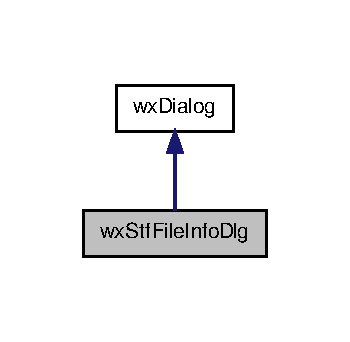
\includegraphics[width=168pt]{classwxStfFileInfoDlg__inherit__graph}
\end{center}
\end{figure}


Collaboration diagram for wxStfFileInfoDlg:
\nopagebreak
\begin{figure}[H]
\begin{center}
\leavevmode
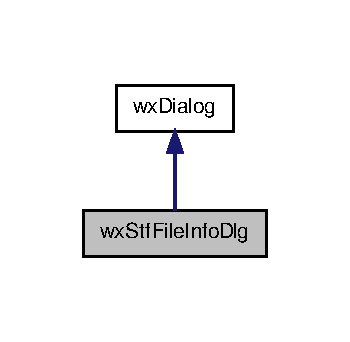
\includegraphics[width=168pt]{classwxStfFileInfoDlg__coll__graph}
\end{center}
\end{figure}
\subsection*{Public Member Functions}
\begin{DoxyCompactItemize}
\item 
\hyperlink{classwxStfFileInfoDlg_aec5a9c07dd33df20112fa6fce63cd1c3}{wxStfFileInfoDlg} (\hyperlink{classwxWindow}{wxWindow} $\ast$parent, const \hyperlink{classwxString}{wxString} \&szGeneral=wxT(\char`\"{}$\backslash$0\char`\"{}), const \hyperlink{classwxString}{wxString} \&szFile=wxT(\char`\"{}$\backslash$0\char`\"{}), const \hyperlink{classwxString}{wxString} \&szSection=wxT(\char`\"{}$\backslash$0\char`\"{}), int id=wxID\_\-ANY, \hyperlink{classwxString}{wxString} title=wxT(\char`\"{}File information\char`\"{}), wxPoint pos=wxDefaultPosition, \hyperlink{classwxSize}{wxSize} size=wxDefaultSize, int style=wxCAPTION)
\begin{DoxyCompactList}\small\item\em Constructor. \item\end{DoxyCompactList}\end{DoxyCompactItemize}


\subsection{Detailed Description}
Dialog showing file information. 

\subsection{Constructor \& Destructor Documentation}
\hypertarget{classwxStfFileInfoDlg_aec5a9c07dd33df20112fa6fce63cd1c3}{
\index{wxStfFileInfoDlg@{wxStfFileInfoDlg}!wxStfFileInfoDlg@{wxStfFileInfoDlg}}
\index{wxStfFileInfoDlg@{wxStfFileInfoDlg}!wxStfFileInfoDlg@{wxStfFileInfoDlg}}
\subsubsection[{wxStfFileInfoDlg}]{\setlength{\rightskip}{0pt plus 5cm}wxStfFileInfoDlg::wxStfFileInfoDlg (
\begin{DoxyParamCaption}
\item[{{\bf wxWindow} $\ast$}]{parent, }
\item[{const {\bf wxString} \&}]{szGeneral = {\ttfamily wxT(\char`\"{}$\backslash$0\char`\"{})}, }
\item[{const {\bf wxString} \&}]{szFile = {\ttfamily wxT(\char`\"{}$\backslash$0\char`\"{})}, }
\item[{const {\bf wxString} \&}]{szSection = {\ttfamily wxT(\char`\"{}$\backslash$0\char`\"{})}, }
\item[{int}]{id = {\ttfamily wxID\_\-ANY}, }
\item[{{\bf wxString}}]{title = {\ttfamily wxT(\char`\"{}File~information\char`\"{})}, }
\item[{{\bf wxPoint}}]{pos = {\ttfamily wxDefaultPosition}, }
\item[{{\bf wxSize}}]{size = {\ttfamily wxDefaultSize}, }
\item[{int}]{style = {\ttfamily wxCAPTION}}
\end{DoxyParamCaption}
)}}
\label{classwxStfFileInfoDlg_aec5a9c07dd33df20112fa6fce63cd1c3}


Constructor. 


\begin{DoxyParams}{Parameters}
{\em parent} & Pointer to parent window. \\
\hline
{\em szGeneral} & General information. \\
\hline
{\em szFile} & File variables information. \\
\hline
{\em szSection} & \hyperlink{classSection}{Section} variable information. \\
\hline
{\em id} & Window id. \\
\hline
{\em title} & Dialog title. \\
\hline
{\em pos} & Initial position. \\
\hline
{\em size} & Initial size. \\
\hline
{\em style} & Dialog style. \\
\hline
\end{DoxyParams}


The documentation for this class was generated from the following file:\begin{DoxyCompactItemize}
\item 
src/app/dlgs/\hyperlink{smalldlgs_8h}{smalldlgs.h}\end{DoxyCompactItemize}

\hypertarget{classwxStfFilterSelDlg}{
\section{wxStfFilterSelDlg Class Reference}
\label{classwxStfFilterSelDlg}\index{wxStfFilterSelDlg@{wxStfFilterSelDlg}}
}


Dialog for selecting a filter function.  




{\ttfamily \#include $<$smalldlgs.h$>$}



Inheritance diagram for wxStfFilterSelDlg:
\nopagebreak
\begin{figure}[H]
\begin{center}
\leavevmode
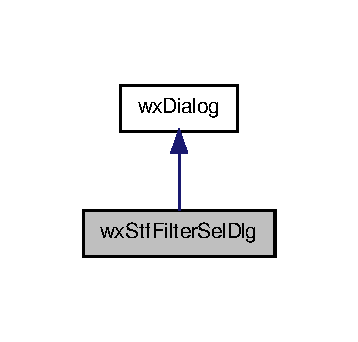
\includegraphics[width=172pt]{classwxStfFilterSelDlg__inherit__graph}
\end{center}
\end{figure}


Collaboration diagram for wxStfFilterSelDlg:
\nopagebreak
\begin{figure}[H]
\begin{center}
\leavevmode
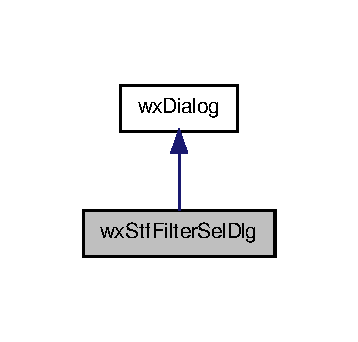
\includegraphics[width=172pt]{classwxStfFilterSelDlg__coll__graph}
\end{center}
\end{figure}
\subsection*{Public Member Functions}
\begin{DoxyCompactItemize}
\item 
\hyperlink{classwxStfFilterSelDlg_a114732c015ccee7e748d3fe9b8e17af3}{wxStfFilterSelDlg} (\hyperlink{classwxWindow}{wxWindow} $\ast$parent, int id=wxID\_\-ANY, \hyperlink{classwxString}{wxString} title=wxT(\char`\"{}Filter function\char`\"{}), wxPoint pos=wxDefaultPosition, \hyperlink{classwxSize}{wxSize} size=wxDefaultSize, int style=wxCAPTION)
\begin{DoxyCompactList}\small\item\em Constructor. \item\end{DoxyCompactList}\item 
int \hyperlink{classwxStfFilterSelDlg_a8ade8a5950d35b39147c43f7058fbc47}{GetFilterSelect} () const 
\begin{DoxyCompactList}\small\item\em Get the selected filter function. \item\end{DoxyCompactList}\item 
virtual void \hyperlink{classwxStfFilterSelDlg_afd36691d17f9e1c9142625823c6eb653}{EndModal} (int retCode)
\begin{DoxyCompactList}\small\item\em Called upon ending a modal dialog. \item\end{DoxyCompactList}\end{DoxyCompactItemize}


\subsection{Detailed Description}
Dialog for selecting a filter function. 

\subsection{Constructor \& Destructor Documentation}
\hypertarget{classwxStfFilterSelDlg_a114732c015ccee7e748d3fe9b8e17af3}{
\index{wxStfFilterSelDlg@{wxStfFilterSelDlg}!wxStfFilterSelDlg@{wxStfFilterSelDlg}}
\index{wxStfFilterSelDlg@{wxStfFilterSelDlg}!wxStfFilterSelDlg@{wxStfFilterSelDlg}}
\subsubsection[{wxStfFilterSelDlg}]{\setlength{\rightskip}{0pt plus 5cm}wxStfFilterSelDlg::wxStfFilterSelDlg (
\begin{DoxyParamCaption}
\item[{{\bf wxWindow} $\ast$}]{parent, }
\item[{int}]{id = {\ttfamily wxID\_\-ANY}, }
\item[{{\bf wxString}}]{title = {\ttfamily wxT(\char`\"{}Filter~function\char`\"{})}, }
\item[{{\bf wxPoint}}]{pos = {\ttfamily wxDefaultPosition}, }
\item[{{\bf wxSize}}]{size = {\ttfamily wxDefaultSize}, }
\item[{int}]{style = {\ttfamily wxCAPTION}}
\end{DoxyParamCaption}
)}}
\label{classwxStfFilterSelDlg_a114732c015ccee7e748d3fe9b8e17af3}


Constructor. 


\begin{DoxyParams}{Parameters}
{\em parent} & Pointer to parent window. \\
\hline
{\em id} & Window id. \\
\hline
{\em title} & Dialog title. \\
\hline
{\em pos} & Initial position. \\
\hline
{\em size} & Initial size. \\
\hline
{\em style} & Dialog style. \\
\hline
\end{DoxyParams}


\subsection{Member Function Documentation}
\hypertarget{classwxStfFilterSelDlg_afd36691d17f9e1c9142625823c6eb653}{
\index{wxStfFilterSelDlg@{wxStfFilterSelDlg}!EndModal@{EndModal}}
\index{EndModal@{EndModal}!wxStfFilterSelDlg@{wxStfFilterSelDlg}}
\subsubsection[{EndModal}]{\setlength{\rightskip}{0pt plus 5cm}virtual void wxStfFilterSelDlg::EndModal (
\begin{DoxyParamCaption}
\item[{int}]{retCode}
\end{DoxyParamCaption}
)\hspace{0.3cm}{\ttfamily  \mbox{[}virtual\mbox{]}}}}
\label{classwxStfFilterSelDlg_afd36691d17f9e1c9142625823c6eb653}


Called upon ending a modal dialog. 


\begin{DoxyParams}{Parameters}
{\em retCode} & The dialog button id that ended the dialog (e.g. wxID\_\-OK) \\
\hline
\end{DoxyParams}
\hypertarget{classwxStfFilterSelDlg_a8ade8a5950d35b39147c43f7058fbc47}{
\index{wxStfFilterSelDlg@{wxStfFilterSelDlg}!GetFilterSelect@{GetFilterSelect}}
\index{GetFilterSelect@{GetFilterSelect}!wxStfFilterSelDlg@{wxStfFilterSelDlg}}
\subsubsection[{GetFilterSelect}]{\setlength{\rightskip}{0pt plus 5cm}int wxStfFilterSelDlg::GetFilterSelect (
\begin{DoxyParamCaption}
{}
\end{DoxyParamCaption}
) const\hspace{0.3cm}{\ttfamily  \mbox{[}inline\mbox{]}}}}
\label{classwxStfFilterSelDlg_a8ade8a5950d35b39147c43f7058fbc47}


Get the selected filter function. 

\begin{DoxyReturn}{Returns}
The index of the selected filter function. 
\end{DoxyReturn}


The documentation for this class was generated from the following file:\begin{DoxyCompactItemize}
\item 
src/app/dlgs/\hyperlink{smalldlgs_8h}{smalldlgs.h}\end{DoxyCompactItemize}

\hypertarget{classwxStfFitInfoDlg}{
\section{wxStfFitInfoDlg Class Reference}
\label{classwxStfFitInfoDlg}\index{wxStfFitInfoDlg@{wxStfFitInfoDlg}}
}


Dialog showing information about a fit.  




{\ttfamily \#include $<$smalldlgs.h$>$}



Inheritance diagram for wxStfFitInfoDlg:
\nopagebreak
\begin{figure}[H]
\begin{center}
\leavevmode
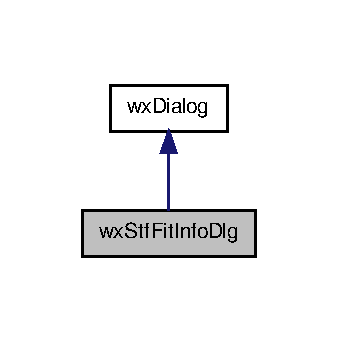
\includegraphics[width=162pt]{classwxStfFitInfoDlg__inherit__graph}
\end{center}
\end{figure}


Collaboration diagram for wxStfFitInfoDlg:
\nopagebreak
\begin{figure}[H]
\begin{center}
\leavevmode
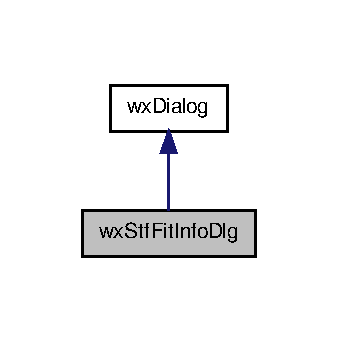
\includegraphics[width=162pt]{classwxStfFitInfoDlg__coll__graph}
\end{center}
\end{figure}
\subsection*{Public Member Functions}
\begin{DoxyCompactItemize}
\item 
\hyperlink{classwxStfFitInfoDlg_a265343d40a13bcab3db9d2ba78a3ecf7}{wxStfFitInfoDlg} (\hyperlink{classwxWindow}{wxWindow} $\ast$parent, const \hyperlink{classwxString}{wxString} \&info, int id=wxID\_\-ANY, \hyperlink{classwxString}{wxString} title=wxT(\char`\"{}Fit information\char`\"{}), wxPoint pos=wxDefaultPosition, \hyperlink{classwxSize}{wxSize} size=wxDefaultSize, int style=wxCAPTION)
\begin{DoxyCompactList}\small\item\em Constructor. \item\end{DoxyCompactList}\end{DoxyCompactItemize}


\subsection{Detailed Description}
Dialog showing information about a fit. 

\subsection{Constructor \& Destructor Documentation}
\hypertarget{classwxStfFitInfoDlg_a265343d40a13bcab3db9d2ba78a3ecf7}{
\index{wxStfFitInfoDlg@{wxStfFitInfoDlg}!wxStfFitInfoDlg@{wxStfFitInfoDlg}}
\index{wxStfFitInfoDlg@{wxStfFitInfoDlg}!wxStfFitInfoDlg@{wxStfFitInfoDlg}}
\subsubsection[{wxStfFitInfoDlg}]{\setlength{\rightskip}{0pt plus 5cm}wxStfFitInfoDlg::wxStfFitInfoDlg (
\begin{DoxyParamCaption}
\item[{{\bf wxWindow} $\ast$}]{parent, }
\item[{const {\bf wxString} \&}]{info, }
\item[{int}]{id = {\ttfamily wxID\_\-ANY}, }
\item[{{\bf wxString}}]{title = {\ttfamily wxT(\char`\"{}Fit~information\char`\"{})}, }
\item[{{\bf wxPoint}}]{pos = {\ttfamily wxDefaultPosition}, }
\item[{{\bf wxSize}}]{size = {\ttfamily wxDefaultSize}, }
\item[{int}]{style = {\ttfamily wxCAPTION}}
\end{DoxyParamCaption}
)}}
\label{classwxStfFitInfoDlg_a265343d40a13bcab3db9d2ba78a3ecf7}


Constructor. 


\begin{DoxyParams}{Parameters}
{\em parent} & Pointer to parent window. \\
\hline
{\em info} & A string containing information about the fit. \\
\hline
{\em id} & Window id. \\
\hline
{\em title} & Dialog title. \\
\hline
{\em pos} & Initial position. \\
\hline
{\em size} & Initial size. \\
\hline
{\em style} & Dialog style. \\
\hline
\end{DoxyParams}


The documentation for this class was generated from the following file:\begin{DoxyCompactItemize}
\item 
src/app/dlgs/\hyperlink{smalldlgs_8h}{smalldlgs.h}\end{DoxyCompactItemize}

\hypertarget{classwxStfFitSelDlg}{
\section{wxStfFitSelDlg Class Reference}
\label{classwxStfFitSelDlg}\index{wxStfFitSelDlg@{wxStfFitSelDlg}}
}


Non-\/linear regression settings dialog.  




{\ttfamily \#include $<$fitseldlg.h$>$}



Inheritance diagram for wxStfFitSelDlg:
\nopagebreak
\begin{figure}[H]
\begin{center}
\leavevmode
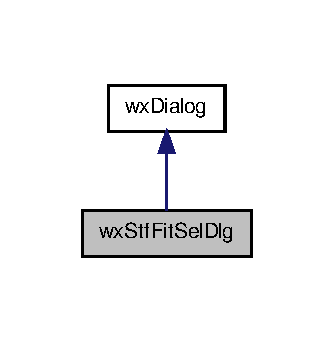
\includegraphics[width=160pt]{classwxStfFitSelDlg__inherit__graph}
\end{center}
\end{figure}


Collaboration diagram for wxStfFitSelDlg:
\nopagebreak
\begin{figure}[H]
\begin{center}
\leavevmode
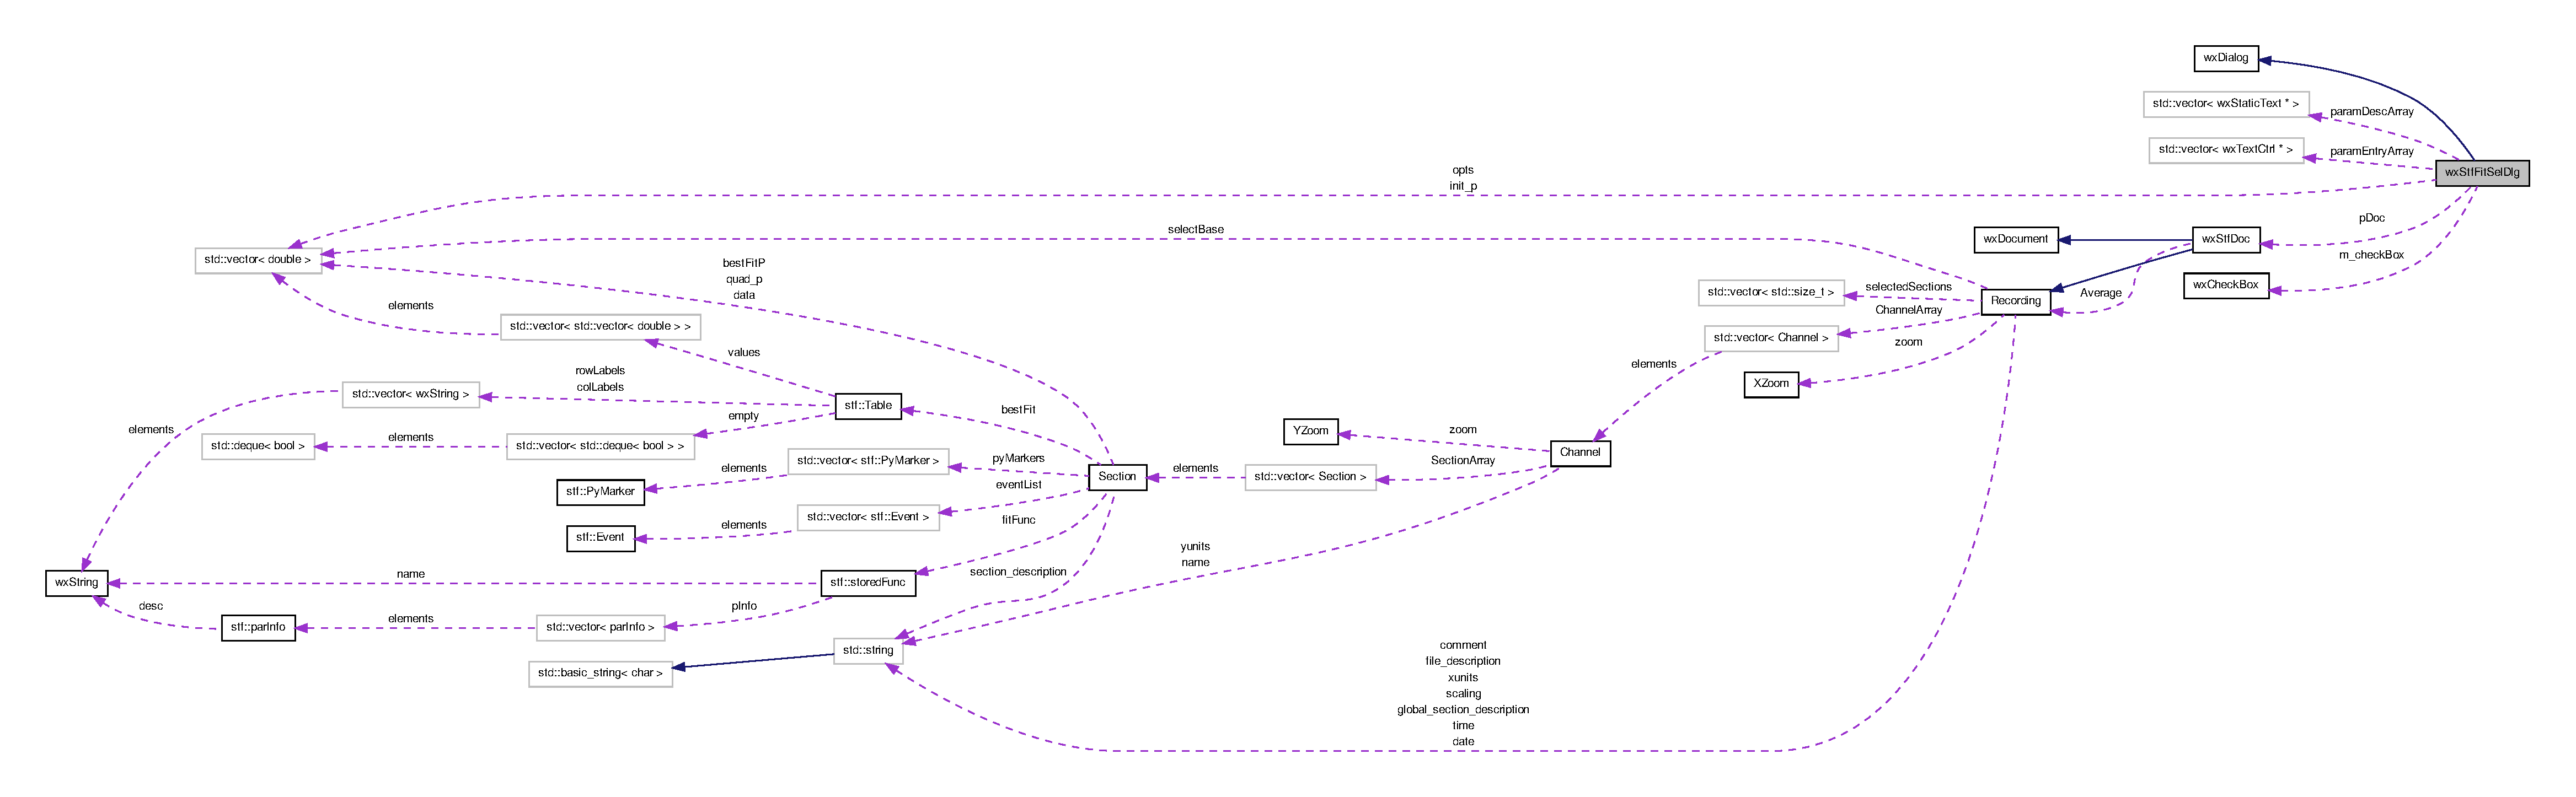
\includegraphics[width=400pt]{classwxStfFitSelDlg__coll__graph}
\end{center}
\end{figure}
\subsection*{Public Member Functions}
\begin{DoxyCompactItemize}
\item 
\hyperlink{classwxStfFitSelDlg_a2c5cf895ab3d5fdea7809beefc0160ff}{wxStfFitSelDlg} (\hyperlink{classwxWindow}{wxWindow} $\ast$parent, \hyperlink{classwxStfDoc}{wxStfDoc} $\ast$doc, int id=wxID\_\-ANY, \hyperlink{classwxString}{wxString} title=wxT(\char`\"{}Non-\/linear regression\char`\"{}), wxPoint pos=wxDefaultPosition, \hyperlink{classwxSize}{wxSize} size=wxDefaultSize, int style=wxCAPTION)
\begin{DoxyCompactList}\small\item\em Constructor. \item\end{DoxyCompactList}\item 
virtual void \hyperlink{classwxStfFitSelDlg_afd1f6cd692c52c7fa27dc98d9db92b2d}{EndModal} (int retCode)
\begin{DoxyCompactList}\small\item\em Called upon ending a modal dialog. \item\end{DoxyCompactList}\item 
int \hyperlink{classwxStfFitSelDlg_abcedd14c33f68da8f69c0ec160ad3472}{GetFSelect} () const 
\begin{DoxyCompactList}\small\item\em Get the selected fit function. \item\end{DoxyCompactList}\item 
Vector\_\-double \hyperlink{classwxStfFitSelDlg_ad5b512cf9138046c51558586938ac481}{GetInitP} () const 
\begin{DoxyCompactList}\small\item\em Get the initial parameters. \item\end{DoxyCompactList}\item 
Vector\_\-double \hyperlink{classwxStfFitSelDlg_a79cc9b1b357bbd49e65cf1ddb39a3e4d}{GetOpts} () const 
\begin{DoxyCompactList}\small\item\em Get options for the algorithm. \item\end{DoxyCompactList}\item 
bool \hyperlink{classwxStfFitSelDlg_af5fa29a748266d7aefd2364b92b4c248}{UseScaling} () const 
\begin{DoxyCompactList}\small\item\em Scale x-\/ and y-\/amplitudes to 1.0 before fit. \item\end{DoxyCompactList}\item 
void \hyperlink{classwxStfFitSelDlg_ad22001ce114a30061d2cf9d4d70b622f}{SetNoInput} (bool noInput\_\-)
\begin{DoxyCompactList}\small\item\em Determines whether user-\/defined initial parameters are allowed. \item\end{DoxyCompactList}\end{DoxyCompactItemize}


\subsection{Detailed Description}
Non-\/linear regression settings dialog. 

\subsection{Constructor \& Destructor Documentation}
\hypertarget{classwxStfFitSelDlg_a2c5cf895ab3d5fdea7809beefc0160ff}{
\index{wxStfFitSelDlg@{wxStfFitSelDlg}!wxStfFitSelDlg@{wxStfFitSelDlg}}
\index{wxStfFitSelDlg@{wxStfFitSelDlg}!wxStfFitSelDlg@{wxStfFitSelDlg}}
\subsubsection[{wxStfFitSelDlg}]{\setlength{\rightskip}{0pt plus 5cm}wxStfFitSelDlg::wxStfFitSelDlg (
\begin{DoxyParamCaption}
\item[{{\bf wxWindow} $\ast$}]{parent, }
\item[{{\bf wxStfDoc} $\ast$}]{doc, }
\item[{int}]{id = {\ttfamily wxID\_\-ANY}, }
\item[{{\bf wxString}}]{title = {\ttfamily wxT(\char`\"{}Non-\/linear~regression\char`\"{})}, }
\item[{{\bf wxPoint}}]{pos = {\ttfamily wxDefaultPosition}, }
\item[{{\bf wxSize}}]{size = {\ttfamily wxDefaultSize}, }
\item[{int}]{style = {\ttfamily wxCAPTION}}
\end{DoxyParamCaption}
)}}
\label{classwxStfFitSelDlg_a2c5cf895ab3d5fdea7809beefc0160ff}


Constructor. 


\begin{DoxyParams}{Parameters}
{\em parent} & Pointer to parent window. \\
\hline
{\em doc} & Pointer to the document the call originated from. \\
\hline
{\em id} & Window id. \\
\hline
{\em title} & Dialog title. \\
\hline
{\em pos} & Initial position. \\
\hline
{\em size} & Initial size. \\
\hline
{\em style} & Dialog style. \\
\hline
\end{DoxyParams}


\subsection{Member Function Documentation}
\hypertarget{classwxStfFitSelDlg_afd1f6cd692c52c7fa27dc98d9db92b2d}{
\index{wxStfFitSelDlg@{wxStfFitSelDlg}!EndModal@{EndModal}}
\index{EndModal@{EndModal}!wxStfFitSelDlg@{wxStfFitSelDlg}}
\subsubsection[{EndModal}]{\setlength{\rightskip}{0pt plus 5cm}virtual void wxStfFitSelDlg::EndModal (
\begin{DoxyParamCaption}
\item[{int}]{retCode}
\end{DoxyParamCaption}
)\hspace{0.3cm}{\ttfamily  \mbox{[}virtual\mbox{]}}}}
\label{classwxStfFitSelDlg_afd1f6cd692c52c7fa27dc98d9db92b2d}


Called upon ending a modal dialog. 


\begin{DoxyParams}{Parameters}
{\em retCode} & The dialog button id that ended the dialog (e.g. wxID\_\-OK) \\
\hline
\end{DoxyParams}
\hypertarget{classwxStfFitSelDlg_abcedd14c33f68da8f69c0ec160ad3472}{
\index{wxStfFitSelDlg@{wxStfFitSelDlg}!GetFSelect@{GetFSelect}}
\index{GetFSelect@{GetFSelect}!wxStfFitSelDlg@{wxStfFitSelDlg}}
\subsubsection[{GetFSelect}]{\setlength{\rightskip}{0pt plus 5cm}int wxStfFitSelDlg::GetFSelect (
\begin{DoxyParamCaption}
{}
\end{DoxyParamCaption}
) const\hspace{0.3cm}{\ttfamily  \mbox{[}inline\mbox{]}}}}
\label{classwxStfFitSelDlg_abcedd14c33f68da8f69c0ec160ad3472}


Get the selected fit function. 

\begin{DoxyReturn}{Returns}
The index of the selected fit function. 
\end{DoxyReturn}
\hypertarget{classwxStfFitSelDlg_ad5b512cf9138046c51558586938ac481}{
\index{wxStfFitSelDlg@{wxStfFitSelDlg}!GetInitP@{GetInitP}}
\index{GetInitP@{GetInitP}!wxStfFitSelDlg@{wxStfFitSelDlg}}
\subsubsection[{GetInitP}]{\setlength{\rightskip}{0pt plus 5cm}Vector\_\-double wxStfFitSelDlg::GetInitP (
\begin{DoxyParamCaption}
{}
\end{DoxyParamCaption}
) const\hspace{0.3cm}{\ttfamily  \mbox{[}inline\mbox{]}}}}
\label{classwxStfFitSelDlg_ad5b512cf9138046c51558586938ac481}


Get the initial parameters. 

\begin{DoxyReturn}{Returns}
A valarray containing the initial parameter set to start the fit. 
\end{DoxyReturn}
\hypertarget{classwxStfFitSelDlg_a79cc9b1b357bbd49e65cf1ddb39a3e4d}{
\index{wxStfFitSelDlg@{wxStfFitSelDlg}!GetOpts@{GetOpts}}
\index{GetOpts@{GetOpts}!wxStfFitSelDlg@{wxStfFitSelDlg}}
\subsubsection[{GetOpts}]{\setlength{\rightskip}{0pt plus 5cm}Vector\_\-double wxStfFitSelDlg::GetOpts (
\begin{DoxyParamCaption}
{}
\end{DoxyParamCaption}
) const\hspace{0.3cm}{\ttfamily  \mbox{[}inline\mbox{]}}}}
\label{classwxStfFitSelDlg_a79cc9b1b357bbd49e65cf1ddb39a3e4d}


Get options for the algorithm. 

\begin{DoxyReturn}{Returns}
A valarray containing the initial parameters for the algorithm. 
\end{DoxyReturn}
\hypertarget{classwxStfFitSelDlg_ad22001ce114a30061d2cf9d4d70b622f}{
\index{wxStfFitSelDlg@{wxStfFitSelDlg}!SetNoInput@{SetNoInput}}
\index{SetNoInput@{SetNoInput}!wxStfFitSelDlg@{wxStfFitSelDlg}}
\subsubsection[{SetNoInput}]{\setlength{\rightskip}{0pt plus 5cm}void wxStfFitSelDlg::SetNoInput (
\begin{DoxyParamCaption}
\item[{bool}]{noInput\_\-}
\end{DoxyParamCaption}
)\hspace{0.3cm}{\ttfamily  \mbox{[}inline\mbox{]}}}}
\label{classwxStfFitSelDlg_ad22001ce114a30061d2cf9d4d70b622f}


Determines whether user-\/defined initial parameters are allowed. 


\begin{DoxyParams}{Parameters}
{\em noInput\_\-} & Set to true if the user may set the initial parameters, false otherwise. Needed for batch analysis. \\
\hline
\end{DoxyParams}
\hypertarget{classwxStfFitSelDlg_af5fa29a748266d7aefd2364b92b4c248}{
\index{wxStfFitSelDlg@{wxStfFitSelDlg}!UseScaling@{UseScaling}}
\index{UseScaling@{UseScaling}!wxStfFitSelDlg@{wxStfFitSelDlg}}
\subsubsection[{UseScaling}]{\setlength{\rightskip}{0pt plus 5cm}bool wxStfFitSelDlg::UseScaling (
\begin{DoxyParamCaption}
{}
\end{DoxyParamCaption}
) const\hspace{0.3cm}{\ttfamily  \mbox{[}inline\mbox{]}}}}
\label{classwxStfFitSelDlg_af5fa29a748266d7aefd2364b92b4c248}


Scale x-\/ and y-\/amplitudes to 1.0 before fit. 

\begin{DoxyReturn}{Returns}
True if scaling should be used 
\end{DoxyReturn}


The documentation for this class was generated from the following file:\begin{DoxyCompactItemize}
\item 
src/app/dlgs/\hyperlink{fitseldlg_8h}{fitseldlg.h}\end{DoxyCompactItemize}

\hypertarget{classwxStfGaussianDlg}{
\section{wxStfGaussianDlg Class Reference}
\label{classwxStfGaussianDlg}\index{wxStfGaussianDlg@{wxStfGaussianDlg}}
}


Dialog for setting the parameters of a Gaussian function.  




{\ttfamily \#include $<$smalldlgs.h$>$}



Inheritance diagram for wxStfGaussianDlg:
\nopagebreak
\begin{figure}[H]
\begin{center}
\leavevmode
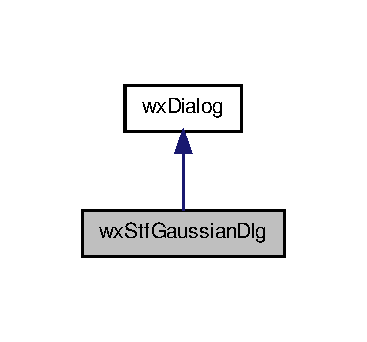
\includegraphics[width=176pt]{classwxStfGaussianDlg__inherit__graph}
\end{center}
\end{figure}


Collaboration diagram for wxStfGaussianDlg:
\nopagebreak
\begin{figure}[H]
\begin{center}
\leavevmode
\includegraphics[width=176pt]{classwxStfGaussianDlg__coll__graph}
\end{center}
\end{figure}
\subsection*{Public Member Functions}
\begin{DoxyCompactItemize}
\item 
\hyperlink{classwxStfGaussianDlg_a0c21a17835300888f0808ba3012e9516}{wxStfGaussianDlg} (\hyperlink{classwxWindow}{wxWindow} $\ast$parent, int id=wxID\_\-ANY, \hyperlink{classwxString}{wxString} title=wxT(\char`\"{}Settings for Gaussian function\char`\"{}), wxPoint pos=wxDefaultPosition, \hyperlink{classwxSize}{wxSize} size=wxDefaultSize, int style=wxCAPTION)
\begin{DoxyCompactList}\small\item\em Constructor. \item\end{DoxyCompactList}\item 
double \hyperlink{classwxStfGaussianDlg_aa35effdf9697f4795f047592af846894}{Width} () const 
\begin{DoxyCompactList}\small\item\em Get the width of the Gaussian. \item\end{DoxyCompactList}\item 
double \hyperlink{classwxStfGaussianDlg_aaead7f642a373594316867193038525b}{Center} () const 
\begin{DoxyCompactList}\small\item\em Get the center of the Gaussian. \item\end{DoxyCompactList}\item 
double \hyperlink{classwxStfGaussianDlg_abfffa79e6088609f367531a267ff9bde}{Amp} () const 
\begin{DoxyCompactList}\small\item\em Get the amplitude of the Gaussian. \item\end{DoxyCompactList}\item 
virtual void \hyperlink{classwxStfGaussianDlg_af51cef0ee1cd2eb515c7bee24b2a5468}{EndModal} (int retCode)
\begin{DoxyCompactList}\small\item\em Called upon ending a modal dialog. \item\end{DoxyCompactList}\end{DoxyCompactItemize}


\subsection{Detailed Description}
Dialog for setting the parameters of a Gaussian function. 

\subsection{Constructor \& Destructor Documentation}
\hypertarget{classwxStfGaussianDlg_a0c21a17835300888f0808ba3012e9516}{
\index{wxStfGaussianDlg@{wxStfGaussianDlg}!wxStfGaussianDlg@{wxStfGaussianDlg}}
\index{wxStfGaussianDlg@{wxStfGaussianDlg}!wxStfGaussianDlg@{wxStfGaussianDlg}}
\subsubsection[{wxStfGaussianDlg}]{\setlength{\rightskip}{0pt plus 5cm}wxStfGaussianDlg::wxStfGaussianDlg (
\begin{DoxyParamCaption}
\item[{{\bf wxWindow} $\ast$}]{parent, }
\item[{int}]{id = {\ttfamily wxID\_\-ANY}, }
\item[{{\bf wxString}}]{title = {\ttfamily wxT(\char`\"{}Settings~for~Gaussian~function\char`\"{})}, }
\item[{{\bf wxPoint}}]{pos = {\ttfamily wxDefaultPosition}, }
\item[{{\bf wxSize}}]{size = {\ttfamily wxDefaultSize}, }
\item[{int}]{style = {\ttfamily wxCAPTION}}
\end{DoxyParamCaption}
)}}
\label{classwxStfGaussianDlg_a0c21a17835300888f0808ba3012e9516}


Constructor. 


\begin{DoxyParams}{Parameters}
{\em parent} & Pointer to parent window. \\
\hline
{\em id} & Window id. \\
\hline
{\em title} & Dialog title. \\
\hline
{\em pos} & Initial position. \\
\hline
{\em size} & Initial size. \\
\hline
{\em style} & Dialog style. \\
\hline
\end{DoxyParams}


\subsection{Member Function Documentation}
\hypertarget{classwxStfGaussianDlg_abfffa79e6088609f367531a267ff9bde}{
\index{wxStfGaussianDlg@{wxStfGaussianDlg}!Amp@{Amp}}
\index{Amp@{Amp}!wxStfGaussianDlg@{wxStfGaussianDlg}}
\subsubsection[{Amp}]{\setlength{\rightskip}{0pt plus 5cm}double wxStfGaussianDlg::Amp (
\begin{DoxyParamCaption}
{}
\end{DoxyParamCaption}
) const\hspace{0.3cm}{\ttfamily  \mbox{[}inline\mbox{]}}}}
\label{classwxStfGaussianDlg_abfffa79e6088609f367531a267ff9bde}


Get the amplitude of the Gaussian. 

\begin{DoxyReturn}{Returns}
The amplitude of the Gaussian. 
\end{DoxyReturn}
\hypertarget{classwxStfGaussianDlg_aaead7f642a373594316867193038525b}{
\index{wxStfGaussianDlg@{wxStfGaussianDlg}!Center@{Center}}
\index{Center@{Center}!wxStfGaussianDlg@{wxStfGaussianDlg}}
\subsubsection[{Center}]{\setlength{\rightskip}{0pt plus 5cm}double wxStfGaussianDlg::Center (
\begin{DoxyParamCaption}
{}
\end{DoxyParamCaption}
) const\hspace{0.3cm}{\ttfamily  \mbox{[}inline\mbox{]}}}}
\label{classwxStfGaussianDlg_aaead7f642a373594316867193038525b}


Get the center of the Gaussian. 

\begin{DoxyReturn}{Returns}
The center of the Gaussian. 
\end{DoxyReturn}
\hypertarget{classwxStfGaussianDlg_af51cef0ee1cd2eb515c7bee24b2a5468}{
\index{wxStfGaussianDlg@{wxStfGaussianDlg}!EndModal@{EndModal}}
\index{EndModal@{EndModal}!wxStfGaussianDlg@{wxStfGaussianDlg}}
\subsubsection[{EndModal}]{\setlength{\rightskip}{0pt plus 5cm}virtual void wxStfGaussianDlg::EndModal (
\begin{DoxyParamCaption}
\item[{int}]{retCode}
\end{DoxyParamCaption}
)\hspace{0.3cm}{\ttfamily  \mbox{[}virtual\mbox{]}}}}
\label{classwxStfGaussianDlg_af51cef0ee1cd2eb515c7bee24b2a5468}


Called upon ending a modal dialog. 


\begin{DoxyParams}{Parameters}
{\em retCode} & The dialog button id that ended the dialog (e.g. wxID\_\-OK) \\
\hline
\end{DoxyParams}
\hypertarget{classwxStfGaussianDlg_aa35effdf9697f4795f047592af846894}{
\index{wxStfGaussianDlg@{wxStfGaussianDlg}!Width@{Width}}
\index{Width@{Width}!wxStfGaussianDlg@{wxStfGaussianDlg}}
\subsubsection[{Width}]{\setlength{\rightskip}{0pt plus 5cm}double wxStfGaussianDlg::Width (
\begin{DoxyParamCaption}
{}
\end{DoxyParamCaption}
) const\hspace{0.3cm}{\ttfamily  \mbox{[}inline\mbox{]}}}}
\label{classwxStfGaussianDlg_aa35effdf9697f4795f047592af846894}


Get the width of the Gaussian. 

\begin{DoxyReturn}{Returns}
The width of the Gaussian. 
\end{DoxyReturn}


The documentation for this class was generated from the following file:\begin{DoxyCompactItemize}
\item 
src/app/dlgs/\hyperlink{smalldlgs_8h}{smalldlgs.h}\end{DoxyCompactItemize}

\hypertarget{classwxStfGraph}{
\section{wxStfGraph Class Reference}
\label{classwxStfGraph}\index{wxStfGraph@{wxStfGraph}}
}


Handles drawing of traces and keyboard or mouse input.  




{\ttfamily \#include $<$graph.h$>$}



Collaboration diagram for wxStfGraph:
\nopagebreak
\begin{figure}[H]
\begin{center}
\leavevmode
\includegraphics[width=400pt]{classwxStfGraph__coll__graph}
\end{center}
\end{figure}
\subsection*{Public Member Functions}
\begin{DoxyCompactItemize}
\item 
\hyperlink{classwxStfGraph_aa19a02121e8240a197ec10a20e3751ca}{wxStfGraph} (\hyperlink{classwxView}{wxView} $\ast$v, \hyperlink{classwxStfChildFrame}{wxStfChildFrame} $\ast$frame, const \hyperlink{classwxPoint}{wxPoint} \&pos, const \hyperlink{classwxSize}{wxSize} \&size, long style)
\begin{DoxyCompactList}\small\item\em Constructor. \item\end{DoxyCompactList}\item 
virtual void \hyperlink{classwxStfGraph_ab22a974e78c974e314949a1f6c04f2bf}{OnDraw} (wxDC \&dc)
\begin{DoxyCompactList}\small\item\em The central drawing function. Used for drawing to any output device, such as a printer or a screen. \item\end{DoxyCompactList}\item 
void \hyperlink{classwxStfGraph_af0c2c4b22e9dd59bfd3b6ba1b0f6f69e}{Snapshotwmf} ()
\begin{DoxyCompactList}\small\item\em Copies the drawing to the clipboard as a windows metafile. \item\end{DoxyCompactList}\item 
void \hyperlink{classwxStfGraph_a445bbe3edaf48c30bbda551a34e2a310}{OnMouseEvent} (wxMouseEvent \&event)
\begin{DoxyCompactList}\small\item\em Handles mouse events. \item\end{DoxyCompactList}\item 
void \hyperlink{classwxStfGraph_adcc0249304ccc1807a99625ce287824b}{OnKeyDown} (wxKeyEvent \&event)
\begin{DoxyCompactList}\small\item\em Handles keyboard input. \item\end{DoxyCompactList}\item 
void \hyperlink{classwxStfGraph_aeef23d32da434baf2e6d711017e4003c}{OnNext} ()
\begin{DoxyCompactList}\small\item\em Show and analyse next trace. \item\end{DoxyCompactList}\item 
void \hyperlink{classwxStfGraph_a7936092de661032f6ceb0373a57b1876}{OnPrevious} ()
\begin{DoxyCompactList}\small\item\em Show and analyse previous trace. \item\end{DoxyCompactList}\item 
void \hyperlink{classwxStfGraph_aa353e7aa0aefef645123a32925e1ca7f}{OnLast} ()
\begin{DoxyCompactList}\small\item\em Show and analyse last trace. \item\end{DoxyCompactList}\item 
void \hyperlink{classwxStfGraph_a201bfc2f8af1928bbe2c2ac393bde623}{OnFirst} ()
\begin{DoxyCompactList}\small\item\em Show and analyse first trace. \item\end{DoxyCompactList}\item 
void \hyperlink{classwxStfGraph_aab8d2886c44369a581363a6c4dfa9a3d}{OnUp} ()
\begin{DoxyCompactList}\small\item\em Moves the traces up by 20 px. \item\end{DoxyCompactList}\item 
void \hyperlink{classwxStfGraph_acb8e9314a98a9b7fa830c85f79911673}{OnDown} ()
\begin{DoxyCompactList}\small\item\em Moves the traces down by 20 px. \item\end{DoxyCompactList}\item 
void \hyperlink{classwxStfGraph_a223c167a1f0ae50855209292172417e1}{OnRight} ()
\begin{DoxyCompactList}\small\item\em Moves the traces right by 20 px. \item\end{DoxyCompactList}\item 
void \hyperlink{classwxStfGraph_aef0d5d13d92a20863c33125a3c797b2f}{OnLeft} ()
\begin{DoxyCompactList}\small\item\em Moves the traces left by 20 px. \item\end{DoxyCompactList}\item 
void \hyperlink{classwxStfGraph_a9dcef0216b9c7eef5db0cf4319c2bd5b}{OnXenlhi} ()
\begin{DoxyCompactList}\small\item\em Enlarges the x-\/scale by a factor of 2. \item\end{DoxyCompactList}\item 
void \hyperlink{classwxStfGraph_a89d5fba83bfd0065f67a0a1ac0c65b09}{OnXenllo} ()
\begin{DoxyCompactList}\small\item\em Enlarges the x-\/scale by a factor of 1.1. \item\end{DoxyCompactList}\item 
void \hyperlink{classwxStfGraph_aa7465a5d3f1304e240a4375eb352ad68}{OnXshrinklo} ()
\begin{DoxyCompactList}\small\item\em Shrinks the x-\/scale by a factor of 1.1. \item\end{DoxyCompactList}\item 
void \hyperlink{classwxStfGraph_a0dc27892670291a85e9b1dd9990be69a}{OnXshrinkhi} ()
\begin{DoxyCompactList}\small\item\em Shrinks the x-\/scale by a factor of 2. \item\end{DoxyCompactList}\item 
void \hyperlink{classwxStfGraph_a10681aa17f96022712906eed32b0b510}{OnYenlhi} ()
\begin{DoxyCompactList}\small\item\em Enlarges the y-\/scale by a factor of 2. \item\end{DoxyCompactList}\item 
void \hyperlink{classwxStfGraph_a1eff713a08c34e8a0b3d80ae9ec99454}{OnYenllo} ()
\begin{DoxyCompactList}\small\item\em Enlarges the y-\/scale by a factor of 1.1. \item\end{DoxyCompactList}\item 
void \hyperlink{classwxStfGraph_ae799f0c3a1160c46f31b311b6b9151ff}{OnYshrinklo} ()
\begin{DoxyCompactList}\small\item\em Shrinks the y-\/scale by a factor of 1.1. \item\end{DoxyCompactList}\item 
void \hyperlink{classwxStfGraph_a99cddff62f64fe497b268d8360ad7ed0}{OnYshrinkhi} ()
\begin{DoxyCompactList}\small\item\em Shrinks the y-\/scale by a factor of 2. \item\end{DoxyCompactList}\item 
\hypertarget{classwxStfGraph_a86c1e7b4a43b2a21287cc74f8ce446d4}{
void \hyperlink{classwxStfGraph_a86c1e7b4a43b2a21287cc74f8ce446d4}{Ch2base} ()}
\label{classwxStfGraph_a86c1e7b4a43b2a21287cc74f8ce446d4}

\begin{DoxyCompactList}\small\item\em Adjust y-\/positioning so that the baselines of channel 1 and 2 are at the same y-\/position. \item\end{DoxyCompactList}\item 
\hypertarget{classwxStfGraph_a37dcb75b857298fa5b7a331e239f78f4}{
void \hyperlink{classwxStfGraph_a37dcb75b857298fa5b7a331e239f78f4}{Ch2pos} ()}
\label{classwxStfGraph_a37dcb75b857298fa5b7a331e239f78f4}

\begin{DoxyCompactList}\small\item\em Adjust y-\/positioning so that channel 1 and 2 are at the same absolute y-\/position. \item\end{DoxyCompactList}\item 
\hypertarget{classwxStfGraph_a4dc6f001a2fdda3d33df44ddbd4511fe}{
void \hyperlink{classwxStfGraph_a4dc6f001a2fdda3d33df44ddbd4511fe}{Ch2zoom} ()}
\label{classwxStfGraph_a4dc6f001a2fdda3d33df44ddbd4511fe}

\begin{DoxyCompactList}\small\item\em Adjust y-\/scale so that channel 1 and 2 have the same y-\/scale. \item\end{DoxyCompactList}\item 
void \hyperlink{classwxStfGraph_ad71175f64d59ebf89f6b44ff8d2e005d}{Ch2basezoom} ()
\begin{DoxyCompactList}\small\item\em Combines \hyperlink{classwxStfGraph_a4dc6f001a2fdda3d33df44ddbd4511fe}{Ch2zoom()} and \hyperlink{classwxStfGraph_a86c1e7b4a43b2a21287cc74f8ce446d4}{Ch2base()}. \item\end{DoxyCompactList}\item 
void \hyperlink{classwxStfGraph_ad9160a9247942883bd183391d4d23ac9}{Fittowindow} (bool refresh)
\begin{DoxyCompactList}\small\item\em Fits the graph to the window. \item\end{DoxyCompactList}\item 
void \hyperlink{classwxStfGraph_a78be138bbfb1f43726ff692898197914}{set\_\-isPrinted} (bool value)
\begin{DoxyCompactList}\small\item\em Set to true if the graph is drawn on a printer. \item\end{DoxyCompactList}\item 
void \hyperlink{classwxStfGraph_a6e1c5275902f8305e6a97ccda210e303}{set\_\-printScale} (double value)
\begin{DoxyCompactList}\small\item\em Sets the printing scale to the specified value. \item\end{DoxyCompactList}\item 
void \hyperlink{classwxStfGraph_a6e46e77d7c75fb9ed44d7d558ee00f3c}{set\_\-printRect} (wxRect value)
\begin{DoxyCompactList}\small\item\em Sets the size of the printout to the epcified rectangle. \item\end{DoxyCompactList}\item 
void \hyperlink{classwxStfGraph_a03c53f826e73b7cb720e8365f14154b9}{set\_\-noGimmicks} (bool value)
\begin{DoxyCompactList}\small\item\em Set to true if the results table and the cursors should be printed. \item\end{DoxyCompactList}\item 
void \hyperlink{classwxStfGraph_ab45c79dfdb70f26741223f1e9f73ed89}{set\_\-downsampling} (int value)
\begin{DoxyCompactList}\small\item\em Prints every n-\/th point. \item\end{DoxyCompactList}\item 
bool \hyperlink{classwxStfGraph_a66565bf1b8c8735ee244201dea518621}{get\_\-noGimmicks} () const 
\begin{DoxyCompactList}\small\item\em Indicates whether everything (cursors, results table, etc.) is printed out. \item\end{DoxyCompactList}\item 
int \hyperlink{classwxStfGraph_a66d4bb8513f5b223478cc70355730b21}{get\_\-eventPos} () const 
\begin{DoxyCompactList}\small\item\em Returns the y-\/position of a right click when in event-\/detection mode. \item\end{DoxyCompactList}\item 
double \hyperlink{classwxStfGraph_a1432014f4eef0a12a075356c3dfcffe9}{get\_\-plot\_\-xmin} () const 
\begin{DoxyCompactList}\small\item\em Returns x value of the left screen border. \item\end{DoxyCompactList}\item 
double \hyperlink{classwxStfGraph_a87e9ef1ebb50844b8094b77edff77768}{get\_\-plot\_\-xmax} () const 
\begin{DoxyCompactList}\small\item\em Returns x value of the right screen border. \item\end{DoxyCompactList}\item 
double \hyperlink{classwxStfGraph_aa1aec4dbf01c1b1325b49d6d48cdaa14}{get\_\-plot\_\-ymin} () const 
\begin{DoxyCompactList}\small\item\em Returns y value of the bottom screen border. \item\end{DoxyCompactList}\item 
double \hyperlink{classwxStfGraph_ae9bb359dc6fd0a8baa36fd347f82dd1a}{get\_\-plot\_\-ymax} () const 
\begin{DoxyCompactList}\small\item\em Returns y value of the top screen border. \item\end{DoxyCompactList}\end{DoxyCompactItemize}
\subsection*{Public Attributes}
\begin{DoxyCompactItemize}
\item 
\hyperlink{classwxStfView}{wxStfView} $\ast$ \hyperlink{classwxStfGraph_aec59dd5424523ad7c8cf42bee83f95d6}{view}
\begin{DoxyCompactList}\small\item\em Returns the current zoom struct. \item\end{DoxyCompactList}\end{DoxyCompactItemize}


\subsection{Detailed Description}
Handles drawing of traces and keyboard or mouse input. Derived from wxScrolledWindow, although no scrolling is implemented at this time. All the trace scaling and drawing happens here. Mouse and keyboard input is handled here as well. 

\subsection{Constructor \& Destructor Documentation}
\hypertarget{classwxStfGraph_aa19a02121e8240a197ec10a20e3751ca}{
\index{wxStfGraph@{wxStfGraph}!wxStfGraph@{wxStfGraph}}
\index{wxStfGraph@{wxStfGraph}!wxStfGraph@{wxStfGraph}}
\subsubsection[{wxStfGraph}]{\setlength{\rightskip}{0pt plus 5cm}wxStfGraph::wxStfGraph (
\begin{DoxyParamCaption}
\item[{{\bf wxView} $\ast$}]{v, }
\item[{{\bf wxStfChildFrame} $\ast$}]{frame, }
\item[{const {\bf wxPoint} \&}]{pos, }
\item[{const {\bf wxSize} \&}]{size, }
\item[{long}]{style}
\end{DoxyParamCaption}
)}}
\label{classwxStfGraph_aa19a02121e8240a197ec10a20e3751ca}


Constructor. 


\begin{DoxyParams}{Parameters}
{\em v} & is a pointer to the attached \hyperlink{classwxView}{wxView}. \\
\hline
{\em frame} & is a pointer to the attached child frame. \\
\hline
{\em pos} & and \\
\hline
{\em size} & indicate the initial position and size of this frame. \\
\hline
{\em style} & is the window style. \\
\hline
\end{DoxyParams}


\subsection{Member Function Documentation}
\hypertarget{classwxStfGraph_ad71175f64d59ebf89f6b44ff8d2e005d}{
\index{wxStfGraph@{wxStfGraph}!Ch2basezoom@{Ch2basezoom}}
\index{Ch2basezoom@{Ch2basezoom}!wxStfGraph@{wxStfGraph}}
\subsubsection[{Ch2basezoom}]{\setlength{\rightskip}{0pt plus 5cm}void wxStfGraph::Ch2basezoom (
\begin{DoxyParamCaption}
{}
\end{DoxyParamCaption}
)}}
\label{classwxStfGraph_ad71175f64d59ebf89f6b44ff8d2e005d}


Combines \hyperlink{classwxStfGraph_a4dc6f001a2fdda3d33df44ddbd4511fe}{Ch2zoom()} and \hyperlink{classwxStfGraph_a86c1e7b4a43b2a21287cc74f8ce446d4}{Ch2base()}. 

This is a separate function so that the graph is not refreshed between adjusting the y-\/scale and the baseline. \hypertarget{classwxStfGraph_ad9160a9247942883bd183391d4d23ac9}{
\index{wxStfGraph@{wxStfGraph}!Fittowindow@{Fittowindow}}
\index{Fittowindow@{Fittowindow}!wxStfGraph@{wxStfGraph}}
\subsubsection[{Fittowindow}]{\setlength{\rightskip}{0pt plus 5cm}void wxStfGraph::Fittowindow (
\begin{DoxyParamCaption}
\item[{bool}]{refresh}
\end{DoxyParamCaption}
)}}
\label{classwxStfGraph_ad9160a9247942883bd183391d4d23ac9}


Fits the graph to the window. 

Fits the graph to 100\% of the width and 50\% of the height of the window and centers it. 
\begin{DoxyParams}{Parameters}
{\em refresh} & Set to true if the graph should be refreshed after fitting it to the window. \\
\hline
\end{DoxyParams}
\hypertarget{classwxStfGraph_a66d4bb8513f5b223478cc70355730b21}{
\index{wxStfGraph@{wxStfGraph}!get\_\-eventPos@{get\_\-eventPos}}
\index{get\_\-eventPos@{get\_\-eventPos}!wxStfGraph@{wxStfGraph}}
\subsubsection[{get\_\-eventPos}]{\setlength{\rightskip}{0pt plus 5cm}int wxStfGraph::get\_\-eventPos (
\begin{DoxyParamCaption}
{}
\end{DoxyParamCaption}
) const\hspace{0.3cm}{\ttfamily  \mbox{[}inline\mbox{]}}}}
\label{classwxStfGraph_a66d4bb8513f5b223478cc70355730b21}


Returns the y-\/position of a right click when in event-\/detection mode. 

\begin{DoxyReturn}{Returns}
the index of the trace that the right-\/click position corresponds to. 
\end{DoxyReturn}
\hypertarget{classwxStfGraph_a66565bf1b8c8735ee244201dea518621}{
\index{wxStfGraph@{wxStfGraph}!get\_\-noGimmicks@{get\_\-noGimmicks}}
\index{get\_\-noGimmicks@{get\_\-noGimmicks}!wxStfGraph@{wxStfGraph}}
\subsubsection[{get\_\-noGimmicks}]{\setlength{\rightskip}{0pt plus 5cm}bool wxStfGraph::get\_\-noGimmicks (
\begin{DoxyParamCaption}
{}
\end{DoxyParamCaption}
) const\hspace{0.3cm}{\ttfamily  \mbox{[}inline\mbox{]}}}}
\label{classwxStfGraph_a66565bf1b8c8735ee244201dea518621}


Indicates whether everything (cursors, results table, etc.) is printed out. 

\begin{DoxyReturn}{Returns}
true if everything is printed out. 
\end{DoxyReturn}
\hypertarget{classwxStfGraph_a87e9ef1ebb50844b8094b77edff77768}{
\index{wxStfGraph@{wxStfGraph}!get\_\-plot\_\-xmax@{get\_\-plot\_\-xmax}}
\index{get\_\-plot\_\-xmax@{get\_\-plot\_\-xmax}!wxStfGraph@{wxStfGraph}}
\subsubsection[{get\_\-plot\_\-xmax}]{\setlength{\rightskip}{0pt plus 5cm}double wxStfGraph::get\_\-plot\_\-xmax (
\begin{DoxyParamCaption}
{}
\end{DoxyParamCaption}
) const}}
\label{classwxStfGraph_a87e9ef1ebb50844b8094b77edff77768}


Returns x value of the right screen border. 

\begin{DoxyReturn}{Returns}
x value of the right screen border 
\end{DoxyReturn}
\hypertarget{classwxStfGraph_a1432014f4eef0a12a075356c3dfcffe9}{
\index{wxStfGraph@{wxStfGraph}!get\_\-plot\_\-xmin@{get\_\-plot\_\-xmin}}
\index{get\_\-plot\_\-xmin@{get\_\-plot\_\-xmin}!wxStfGraph@{wxStfGraph}}
\subsubsection[{get\_\-plot\_\-xmin}]{\setlength{\rightskip}{0pt plus 5cm}double wxStfGraph::get\_\-plot\_\-xmin (
\begin{DoxyParamCaption}
{}
\end{DoxyParamCaption}
) const}}
\label{classwxStfGraph_a1432014f4eef0a12a075356c3dfcffe9}


Returns x value of the left screen border. 

\begin{DoxyReturn}{Returns}
x value of the left screen border 
\end{DoxyReturn}
\hypertarget{classwxStfGraph_ae9bb359dc6fd0a8baa36fd347f82dd1a}{
\index{wxStfGraph@{wxStfGraph}!get\_\-plot\_\-ymax@{get\_\-plot\_\-ymax}}
\index{get\_\-plot\_\-ymax@{get\_\-plot\_\-ymax}!wxStfGraph@{wxStfGraph}}
\subsubsection[{get\_\-plot\_\-ymax}]{\setlength{\rightskip}{0pt plus 5cm}double wxStfGraph::get\_\-plot\_\-ymax (
\begin{DoxyParamCaption}
{}
\end{DoxyParamCaption}
) const}}
\label{classwxStfGraph_ae9bb359dc6fd0a8baa36fd347f82dd1a}


Returns y value of the top screen border. 

\begin{DoxyReturn}{Returns}
y value of the top screen border 
\end{DoxyReturn}
\hypertarget{classwxStfGraph_aa1aec4dbf01c1b1325b49d6d48cdaa14}{
\index{wxStfGraph@{wxStfGraph}!get\_\-plot\_\-ymin@{get\_\-plot\_\-ymin}}
\index{get\_\-plot\_\-ymin@{get\_\-plot\_\-ymin}!wxStfGraph@{wxStfGraph}}
\subsubsection[{get\_\-plot\_\-ymin}]{\setlength{\rightskip}{0pt plus 5cm}double wxStfGraph::get\_\-plot\_\-ymin (
\begin{DoxyParamCaption}
{}
\end{DoxyParamCaption}
) const}}
\label{classwxStfGraph_aa1aec4dbf01c1b1325b49d6d48cdaa14}


Returns y value of the bottom screen border. 

\begin{DoxyReturn}{Returns}
y value of the bottom screen border 
\end{DoxyReturn}
\hypertarget{classwxStfGraph_acb8e9314a98a9b7fa830c85f79911673}{
\index{wxStfGraph@{wxStfGraph}!OnDown@{OnDown}}
\index{OnDown@{OnDown}!wxStfGraph@{wxStfGraph}}
\subsubsection[{OnDown}]{\setlength{\rightskip}{0pt plus 5cm}void wxStfGraph::OnDown (
\begin{DoxyParamCaption}
{}
\end{DoxyParamCaption}
)}}
\label{classwxStfGraph_acb8e9314a98a9b7fa830c85f79911673}


Moves the traces down by 20 px. 

Called when either the down arrow cursor key is pressed or the \char`\"{}Move traces down\char`\"{}-\/button is clicked. \hypertarget{classwxStfGraph_ab22a974e78c974e314949a1f6c04f2bf}{
\index{wxStfGraph@{wxStfGraph}!OnDraw@{OnDraw}}
\index{OnDraw@{OnDraw}!wxStfGraph@{wxStfGraph}}
\subsubsection[{OnDraw}]{\setlength{\rightskip}{0pt plus 5cm}virtual void wxStfGraph::OnDraw (
\begin{DoxyParamCaption}
\item[{wxDC \&}]{dc}
\end{DoxyParamCaption}
)\hspace{0.3cm}{\ttfamily  \mbox{[}virtual\mbox{]}}}}
\label{classwxStfGraph_ab22a974e78c974e314949a1f6c04f2bf}


The central drawing function. Used for drawing to any output device, such as a printer or a screen. 


\begin{DoxyParams}{Parameters}
{\em dc} & is the device context used for drawing (can be a printer, a screen or a file). \\
\hline
\end{DoxyParams}
\hypertarget{classwxStfGraph_a201bfc2f8af1928bbe2c2ac393bde623}{
\index{wxStfGraph@{wxStfGraph}!OnFirst@{OnFirst}}
\index{OnFirst@{OnFirst}!wxStfGraph@{wxStfGraph}}
\subsubsection[{OnFirst}]{\setlength{\rightskip}{0pt plus 5cm}void wxStfGraph::OnFirst (
\begin{DoxyParamCaption}
{}
\end{DoxyParamCaption}
)}}
\label{classwxStfGraph_a201bfc2f8af1928bbe2c2ac393bde623}


Show and analyse first trace. 

Called when the \char`\"{}first trace\char`\"{}-\/button is clicked. \hypertarget{classwxStfGraph_adcc0249304ccc1807a99625ce287824b}{
\index{wxStfGraph@{wxStfGraph}!OnKeyDown@{OnKeyDown}}
\index{OnKeyDown@{OnKeyDown}!wxStfGraph@{wxStfGraph}}
\subsubsection[{OnKeyDown}]{\setlength{\rightskip}{0pt plus 5cm}void wxStfGraph::OnKeyDown (
\begin{DoxyParamCaption}
\item[{wxKeyEvent \&}]{event}
\end{DoxyParamCaption}
)}}
\label{classwxStfGraph_adcc0249304ccc1807a99625ce287824b}


Handles keyboard input. 

Key modifiers (e.g. Shift or Ctrl) ar handled within this function. 
\begin{DoxyParams}{Parameters}
{\em event} & The keyboard event. Contains information about the key that was pressed. \\
\hline
\end{DoxyParams}
\hypertarget{classwxStfGraph_aa353e7aa0aefef645123a32925e1ca7f}{
\index{wxStfGraph@{wxStfGraph}!OnLast@{OnLast}}
\index{OnLast@{OnLast}!wxStfGraph@{wxStfGraph}}
\subsubsection[{OnLast}]{\setlength{\rightskip}{0pt plus 5cm}void wxStfGraph::OnLast (
\begin{DoxyParamCaption}
{}
\end{DoxyParamCaption}
)}}
\label{classwxStfGraph_aa353e7aa0aefef645123a32925e1ca7f}


Show and analyse last trace. 

Called when the \char`\"{}last trace\char`\"{}-\/button is clicked. \hypertarget{classwxStfGraph_aef0d5d13d92a20863c33125a3c797b2f}{
\index{wxStfGraph@{wxStfGraph}!OnLeft@{OnLeft}}
\index{OnLeft@{OnLeft}!wxStfGraph@{wxStfGraph}}
\subsubsection[{OnLeft}]{\setlength{\rightskip}{0pt plus 5cm}void wxStfGraph::OnLeft (
\begin{DoxyParamCaption}
{}
\end{DoxyParamCaption}
)}}
\label{classwxStfGraph_aef0d5d13d92a20863c33125a3c797b2f}


Moves the traces left by 20 px. 

Called when either the left arrow cursor key and Ctrl are pressed at the same time or the \char`\"{}Move traces left\char`\"{}-\/button is clicked. \hypertarget{classwxStfGraph_a445bbe3edaf48c30bbda551a34e2a310}{
\index{wxStfGraph@{wxStfGraph}!OnMouseEvent@{OnMouseEvent}}
\index{OnMouseEvent@{OnMouseEvent}!wxStfGraph@{wxStfGraph}}
\subsubsection[{OnMouseEvent}]{\setlength{\rightskip}{0pt plus 5cm}void wxStfGraph::OnMouseEvent (
\begin{DoxyParamCaption}
\item[{wxMouseEvent \&}]{event}
\end{DoxyParamCaption}
)}}
\label{classwxStfGraph_a445bbe3edaf48c30bbda551a34e2a310}


Handles mouse events. 

The different possibilities (e.g. left or right click) split up within this function. 
\begin{DoxyParams}{Parameters}
{\em event} & The mouse event. Contains information such as whether the left or right button was clicked. \\
\hline
\end{DoxyParams}
\hypertarget{classwxStfGraph_aeef23d32da434baf2e6d711017e4003c}{
\index{wxStfGraph@{wxStfGraph}!OnNext@{OnNext}}
\index{OnNext@{OnNext}!wxStfGraph@{wxStfGraph}}
\subsubsection[{OnNext}]{\setlength{\rightskip}{0pt plus 5cm}void wxStfGraph::OnNext (
\begin{DoxyParamCaption}
{}
\end{DoxyParamCaption}
)}}
\label{classwxStfGraph_aeef23d32da434baf2e6d711017e4003c}


Show and analyse next trace. 

Called when either the \char`\"{}next trace\char`\"{}-\/button is clicked or the right arrow cursor key is pressed. Wraps around when last trace is reached. \hypertarget{classwxStfGraph_a7936092de661032f6ceb0373a57b1876}{
\index{wxStfGraph@{wxStfGraph}!OnPrevious@{OnPrevious}}
\index{OnPrevious@{OnPrevious}!wxStfGraph@{wxStfGraph}}
\subsubsection[{OnPrevious}]{\setlength{\rightskip}{0pt plus 5cm}void wxStfGraph::OnPrevious (
\begin{DoxyParamCaption}
{}
\end{DoxyParamCaption}
)}}
\label{classwxStfGraph_a7936092de661032f6ceb0373a57b1876}


Show and analyse previous trace. 

Called when either the \char`\"{}previous trace\char`\"{}-\/button is clicked or the left arrow cursor key is pressed. Wraps around when first trace is reached. \hypertarget{classwxStfGraph_a223c167a1f0ae50855209292172417e1}{
\index{wxStfGraph@{wxStfGraph}!OnRight@{OnRight}}
\index{OnRight@{OnRight}!wxStfGraph@{wxStfGraph}}
\subsubsection[{OnRight}]{\setlength{\rightskip}{0pt plus 5cm}void wxStfGraph::OnRight (
\begin{DoxyParamCaption}
{}
\end{DoxyParamCaption}
)}}
\label{classwxStfGraph_a223c167a1f0ae50855209292172417e1}


Moves the traces right by 20 px. 

Called when either the right arrow cursor key and Ctrl are pressed at the same time or the \char`\"{}Move traces right\char`\"{}-\/button is clicked. \hypertarget{classwxStfGraph_aab8d2886c44369a581363a6c4dfa9a3d}{
\index{wxStfGraph@{wxStfGraph}!OnUp@{OnUp}}
\index{OnUp@{OnUp}!wxStfGraph@{wxStfGraph}}
\subsubsection[{OnUp}]{\setlength{\rightskip}{0pt plus 5cm}void wxStfGraph::OnUp (
\begin{DoxyParamCaption}
{}
\end{DoxyParamCaption}
)}}
\label{classwxStfGraph_aab8d2886c44369a581363a6c4dfa9a3d}


Moves the traces up by 20 px. 

Called when either the up arrow cursor key is pressed or the \char`\"{}Move traces up\char`\"{}-\/button is clicked. \hypertarget{classwxStfGraph_a9dcef0216b9c7eef5db0cf4319c2bd5b}{
\index{wxStfGraph@{wxStfGraph}!OnXenlhi@{OnXenlhi}}
\index{OnXenlhi@{OnXenlhi}!wxStfGraph@{wxStfGraph}}
\subsubsection[{OnXenlhi}]{\setlength{\rightskip}{0pt plus 5cm}void wxStfGraph::OnXenlhi (
\begin{DoxyParamCaption}
{}
\end{DoxyParamCaption}
)}}
\label{classwxStfGraph_a9dcef0216b9c7eef5db0cf4319c2bd5b}


Enlarges the x-\/scale by a factor of 2. 

This is currently never called and might be removed in the future. \hypertarget{classwxStfGraph_a89d5fba83bfd0065f67a0a1ac0c65b09}{
\index{wxStfGraph@{wxStfGraph}!OnXenllo@{OnXenllo}}
\index{OnXenllo@{OnXenllo}!wxStfGraph@{wxStfGraph}}
\subsubsection[{OnXenllo}]{\setlength{\rightskip}{0pt plus 5cm}void wxStfGraph::OnXenllo (
\begin{DoxyParamCaption}
{}
\end{DoxyParamCaption}
)}}
\label{classwxStfGraph_a89d5fba83bfd0065f67a0a1ac0c65b09}


Enlarges the x-\/scale by a factor of 1.1. 

Called when either the \char`\"{}+\char`\"{} key and Ctrl are pressed at the same time or the \char`\"{}Enlarge x-\/scale\char`\"{}-\/button is clicked. \hypertarget{classwxStfGraph_a0dc27892670291a85e9b1dd9990be69a}{
\index{wxStfGraph@{wxStfGraph}!OnXshrinkhi@{OnXshrinkhi}}
\index{OnXshrinkhi@{OnXshrinkhi}!wxStfGraph@{wxStfGraph}}
\subsubsection[{OnXshrinkhi}]{\setlength{\rightskip}{0pt plus 5cm}void wxStfGraph::OnXshrinkhi (
\begin{DoxyParamCaption}
{}
\end{DoxyParamCaption}
)}}
\label{classwxStfGraph_a0dc27892670291a85e9b1dd9990be69a}


Shrinks the x-\/scale by a factor of 2. 

This is currently never called and might be removed in the future. \hypertarget{classwxStfGraph_aa7465a5d3f1304e240a4375eb352ad68}{
\index{wxStfGraph@{wxStfGraph}!OnXshrinklo@{OnXshrinklo}}
\index{OnXshrinklo@{OnXshrinklo}!wxStfGraph@{wxStfGraph}}
\subsubsection[{OnXshrinklo}]{\setlength{\rightskip}{0pt plus 5cm}void wxStfGraph::OnXshrinklo (
\begin{DoxyParamCaption}
{}
\end{DoxyParamCaption}
)}}
\label{classwxStfGraph_aa7465a5d3f1304e240a4375eb352ad68}


Shrinks the x-\/scale by a factor of 1.1. 

Called when either the \char`\"{}-\/\char`\"{} key and Ctrl are pressed at the same time or the \char`\"{}Shrink x-\/scale\char`\"{}-\/button is clicked. \hypertarget{classwxStfGraph_a10681aa17f96022712906eed32b0b510}{
\index{wxStfGraph@{wxStfGraph}!OnYenlhi@{OnYenlhi}}
\index{OnYenlhi@{OnYenlhi}!wxStfGraph@{wxStfGraph}}
\subsubsection[{OnYenlhi}]{\setlength{\rightskip}{0pt plus 5cm}void wxStfGraph::OnYenlhi (
\begin{DoxyParamCaption}
{}
\end{DoxyParamCaption}
)}}
\label{classwxStfGraph_a10681aa17f96022712906eed32b0b510}


Enlarges the y-\/scale by a factor of 2. 

This is currently never called and might be removed in the future. \hypertarget{classwxStfGraph_a1eff713a08c34e8a0b3d80ae9ec99454}{
\index{wxStfGraph@{wxStfGraph}!OnYenllo@{OnYenllo}}
\index{OnYenllo@{OnYenllo}!wxStfGraph@{wxStfGraph}}
\subsubsection[{OnYenllo}]{\setlength{\rightskip}{0pt plus 5cm}void wxStfGraph::OnYenllo (
\begin{DoxyParamCaption}
{}
\end{DoxyParamCaption}
)}}
\label{classwxStfGraph_a1eff713a08c34e8a0b3d80ae9ec99454}


Enlarges the y-\/scale by a factor of 1.1. 

Called when either the \char`\"{}+\char`\"{} key is pressed or the \char`\"{}Enlarge x-\/scale\char`\"{}-\/button is clicked. \hypertarget{classwxStfGraph_a99cddff62f64fe497b268d8360ad7ed0}{
\index{wxStfGraph@{wxStfGraph}!OnYshrinkhi@{OnYshrinkhi}}
\index{OnYshrinkhi@{OnYshrinkhi}!wxStfGraph@{wxStfGraph}}
\subsubsection[{OnYshrinkhi}]{\setlength{\rightskip}{0pt plus 5cm}void wxStfGraph::OnYshrinkhi (
\begin{DoxyParamCaption}
{}
\end{DoxyParamCaption}
)}}
\label{classwxStfGraph_a99cddff62f64fe497b268d8360ad7ed0}


Shrinks the y-\/scale by a factor of 2. 

This is currently never called and might be removed in the future. \hypertarget{classwxStfGraph_ae799f0c3a1160c46f31b311b6b9151ff}{
\index{wxStfGraph@{wxStfGraph}!OnYshrinklo@{OnYshrinklo}}
\index{OnYshrinklo@{OnYshrinklo}!wxStfGraph@{wxStfGraph}}
\subsubsection[{OnYshrinklo}]{\setlength{\rightskip}{0pt plus 5cm}void wxStfGraph::OnYshrinklo (
\begin{DoxyParamCaption}
{}
\end{DoxyParamCaption}
)}}
\label{classwxStfGraph_ae799f0c3a1160c46f31b311b6b9151ff}


Shrinks the y-\/scale by a factor of 1.1. 

Called when either the \char`\"{}-\/\char`\"{} key is pressed or the \char`\"{}Shrink x-\/scale\char`\"{}-\/button is clicked. \hypertarget{classwxStfGraph_ab45c79dfdb70f26741223f1e9f73ed89}{
\index{wxStfGraph@{wxStfGraph}!set\_\-downsampling@{set\_\-downsampling}}
\index{set\_\-downsampling@{set\_\-downsampling}!wxStfGraph@{wxStfGraph}}
\subsubsection[{set\_\-downsampling}]{\setlength{\rightskip}{0pt plus 5cm}void wxStfGraph::set\_\-downsampling (
\begin{DoxyParamCaption}
\item[{int}]{value}
\end{DoxyParamCaption}
)\hspace{0.3cm}{\ttfamily  \mbox{[}inline\mbox{]}}}}
\label{classwxStfGraph_ab45c79dfdb70f26741223f1e9f73ed89}


Prints every n-\/th point. 


\begin{DoxyParams}{Parameters}
{\em value} & Determines that every n-\/th point should be printed. \\
\hline
\end{DoxyParams}
\hypertarget{classwxStfGraph_a78be138bbfb1f43726ff692898197914}{
\index{wxStfGraph@{wxStfGraph}!set\_\-isPrinted@{set\_\-isPrinted}}
\index{set\_\-isPrinted@{set\_\-isPrinted}!wxStfGraph@{wxStfGraph}}
\subsubsection[{set\_\-isPrinted}]{\setlength{\rightskip}{0pt plus 5cm}void wxStfGraph::set\_\-isPrinted (
\begin{DoxyParamCaption}
\item[{bool}]{value}
\end{DoxyParamCaption}
)}}
\label{classwxStfGraph_a78be138bbfb1f43726ff692898197914}


Set to true if the graph is drawn on a printer. 


\begin{DoxyParams}{Parameters}
{\em value} & boolean determining whether the graph is printed. \\
\hline
\end{DoxyParams}
\hypertarget{classwxStfGraph_a03c53f826e73b7cb720e8365f14154b9}{
\index{wxStfGraph@{wxStfGraph}!set\_\-noGimmicks@{set\_\-noGimmicks}}
\index{set\_\-noGimmicks@{set\_\-noGimmicks}!wxStfGraph@{wxStfGraph}}
\subsubsection[{set\_\-noGimmicks}]{\setlength{\rightskip}{0pt plus 5cm}void wxStfGraph::set\_\-noGimmicks (
\begin{DoxyParamCaption}
\item[{bool}]{value}
\end{DoxyParamCaption}
)\hspace{0.3cm}{\ttfamily  \mbox{[}inline\mbox{]}}}}
\label{classwxStfGraph_a03c53f826e73b7cb720e8365f14154b9}


Set to true if the results table and the cursors should be printed. 


\begin{DoxyParams}{Parameters}
{\em value} & boolean determining whether everything should be printed. \\
\hline
\end{DoxyParams}
\hypertarget{classwxStfGraph_a6e46e77d7c75fb9ed44d7d558ee00f3c}{
\index{wxStfGraph@{wxStfGraph}!set\_\-printRect@{set\_\-printRect}}
\index{set\_\-printRect@{set\_\-printRect}!wxStfGraph@{wxStfGraph}}
\subsubsection[{set\_\-printRect}]{\setlength{\rightskip}{0pt plus 5cm}void wxStfGraph::set\_\-printRect (
\begin{DoxyParamCaption}
\item[{wxRect}]{value}
\end{DoxyParamCaption}
)\hspace{0.3cm}{\ttfamily  \mbox{[}inline\mbox{]}}}}
\label{classwxStfGraph_a6e46e77d7c75fb9ed44d7d558ee00f3c}


Sets the size of the printout to the epcified rectangle. 


\begin{DoxyParams}{Parameters}
{\em value} & The new printing rectangle. \\
\hline
\end{DoxyParams}
\hypertarget{classwxStfGraph_a6e1c5275902f8305e6a97ccda210e303}{
\index{wxStfGraph@{wxStfGraph}!set\_\-printScale@{set\_\-printScale}}
\index{set\_\-printScale@{set\_\-printScale}!wxStfGraph@{wxStfGraph}}
\subsubsection[{set\_\-printScale}]{\setlength{\rightskip}{0pt plus 5cm}void wxStfGraph::set\_\-printScale (
\begin{DoxyParamCaption}
\item[{double}]{value}
\end{DoxyParamCaption}
)\hspace{0.3cm}{\ttfamily  \mbox{[}inline\mbox{]}}}}
\label{classwxStfGraph_a6e1c5275902f8305e6a97ccda210e303}


Sets the printing scale to the specified value. 


\begin{DoxyParams}{Parameters}
{\em value} & The new printing scale. \\
\hline
\end{DoxyParams}
\hypertarget{classwxStfGraph_af0c2c4b22e9dd59bfd3b6ba1b0f6f69e}{
\index{wxStfGraph@{wxStfGraph}!Snapshotwmf@{Snapshotwmf}}
\index{Snapshotwmf@{Snapshotwmf}!wxStfGraph@{wxStfGraph}}
\subsubsection[{Snapshotwmf}]{\setlength{\rightskip}{0pt plus 5cm}void wxStfGraph::Snapshotwmf (
\begin{DoxyParamCaption}
{}
\end{DoxyParamCaption}
)}}
\label{classwxStfGraph_af0c2c4b22e9dd59bfd3b6ba1b0f6f69e}


Copies the drawing to the clipboard as a windows metafile. 

Metafiles are only implemented in Windows. Some applications allow you to paste as an enhanced metafile (usually through \char`\"{}Edit -\/$>$ Paste special...\char`\"{}); choose this option for best results. 

\subsection{Member Data Documentation}
\hypertarget{classwxStfGraph_aec59dd5424523ad7c8cf42bee83f95d6}{
\index{wxStfGraph@{wxStfGraph}!view@{view}}
\index{view@{view}!wxStfGraph@{wxStfGraph}}
\subsubsection[{view}]{\setlength{\rightskip}{0pt plus 5cm}{\bf wxStfView}$\ast$ {\bf wxStfGraph::view}}}
\label{classwxStfGraph_aec59dd5424523ad7c8cf42bee83f95d6}


Returns the current zoom struct. 

\begin{DoxyReturn}{Returns}
the current zoom struct. Sets the current zoom struct.
\end{DoxyReturn}

\begin{DoxyParams}{Parameters}
{\em zoom\_\-} & The current zoom struct. The view attached to this \hyperlink{classwxStfGraph}{wxStfGraph}. \\
\hline
\end{DoxyParams}


The documentation for this class was generated from the following file:\begin{DoxyCompactItemize}
\item 
src/app/\hyperlink{graph_8h}{graph.h}\end{DoxyCompactItemize}

\hypertarget{classwxStfGrid}{
\section{wxStfGrid Class Reference}
\label{classwxStfGrid}\index{wxStfGrid@{wxStfGrid}}
}


Derived from \hyperlink{classwxGrid}{wxGrid}. Allows to copy cells to the clipboard.  




{\ttfamily \#include $<$copygrid.h$>$}



Inheritance diagram for wxStfGrid:
\nopagebreak
\begin{figure}[H]
\begin{center}
\leavevmode
\includegraphics[width=138pt]{classwxStfGrid__inherit__graph}
\end{center}
\end{figure}


Collaboration diagram for wxStfGrid:
\nopagebreak
\begin{figure}[H]
\begin{center}
\leavevmode
\includegraphics[width=198pt]{classwxStfGrid__coll__graph}
\end{center}
\end{figure}
\subsection*{Public Member Functions}
\begin{DoxyCompactItemize}
\item 
\hyperlink{classwxStfGrid_a469183f48d70d8d6bd07d7da44c20521}{wxStfGrid} (\hyperlink{classwxWindow}{wxWindow} $\ast$parent, wxWindowID id, const \hyperlink{classwxPoint}{wxPoint} \&pos=wxDefaultPosition, const \hyperlink{classwxSize}{wxSize} \&size=wxDefaultSize, long style=wxWANTS\_\-CHARS, const \hyperlink{classwxString}{wxString} \&name=wxGridNameStr)
\begin{DoxyCompactList}\small\item\em Constructor. \item\end{DoxyCompactList}\item 
\hyperlink{classwxString}{wxString} \hyperlink{classwxStfGrid_a0ad171ef7c2f3a1fbc8f708edb01494f}{GetSelection} () const 
\begin{DoxyCompactList}\small\item\em Get the selection. \item\end{DoxyCompactList}\item 
wxMenu $\ast$ \hyperlink{classwxStfGrid_afb599416fa180751b1c5d1926419c0d7}{get\_\-labelMenu} ()
\item 
\hypertarget{classwxStfGrid_ac4b9bb5f6e5609fcaf96a5bf805c2b11}{
void \hyperlink{classwxStfGrid_ac4b9bb5f6e5609fcaf96a5bf805c2b11}{ViewResults} ()}
\label{classwxStfGrid_ac4b9bb5f6e5609fcaf96a5bf805c2b11}

\begin{DoxyCompactList}\small\item\em Updates the context menu. \item\end{DoxyCompactList}\end{DoxyCompactItemize}


\subsection{Detailed Description}
Derived from \hyperlink{classwxGrid}{wxGrid}. Allows to copy cells to the clipboard. 

\subsection{Constructor \& Destructor Documentation}
\hypertarget{classwxStfGrid_a469183f48d70d8d6bd07d7da44c20521}{
\index{wxStfGrid@{wxStfGrid}!wxStfGrid@{wxStfGrid}}
\index{wxStfGrid@{wxStfGrid}!wxStfGrid@{wxStfGrid}}
\subsubsection[{wxStfGrid}]{\setlength{\rightskip}{0pt plus 5cm}wxStfGrid::wxStfGrid (
\begin{DoxyParamCaption}
\item[{{\bf wxWindow} $\ast$}]{parent, }
\item[{wxWindowID}]{id, }
\item[{const {\bf wxPoint} \&}]{pos = {\ttfamily wxDefaultPosition}, }
\item[{const {\bf wxSize} \&}]{size = {\ttfamily wxDefaultSize}, }
\item[{long}]{style = {\ttfamily wxWANTS\_\-CHARS}, }
\item[{const {\bf wxString} \&}]{name = {\ttfamily wxGridNameStr}}
\end{DoxyParamCaption}
)}}
\label{classwxStfGrid_a469183f48d70d8d6bd07d7da44c20521}


Constructor. 


\begin{DoxyParams}{Parameters}
{\em parent} & Pointer to the parent window. \\
\hline
{\em id} & Window id. \\
\hline
{\em pos} & Initial window position. \\
\hline
{\em size} & Initial window size. \\
\hline
{\em style} & Grid style. \\
\hline
{\em name} & Name of this grid. \\
\hline
\end{DoxyParams}


\subsection{Member Function Documentation}
\hypertarget{classwxStfGrid_afb599416fa180751b1c5d1926419c0d7}{
\index{wxStfGrid@{wxStfGrid}!get\_\-labelMenu@{get\_\-labelMenu}}
\index{get\_\-labelMenu@{get\_\-labelMenu}!wxStfGrid@{wxStfGrid}}
\subsubsection[{get\_\-labelMenu}]{\setlength{\rightskip}{0pt plus 5cm}wxMenu$\ast$ wxStfGrid::get\_\-labelMenu (
\begin{DoxyParamCaption}
{}
\end{DoxyParamCaption}
)\hspace{0.3cm}{\ttfamily  \mbox{[}inline\mbox{]}}}}
\label{classwxStfGrid_afb599416fa180751b1c5d1926419c0d7}
\begin{DoxyReturn}{Returns}
A pointer to the context menu. 
\end{DoxyReturn}
\hypertarget{classwxStfGrid_a0ad171ef7c2f3a1fbc8f708edb01494f}{
\index{wxStfGrid@{wxStfGrid}!GetSelection@{GetSelection}}
\index{GetSelection@{GetSelection}!wxStfGrid@{wxStfGrid}}
\subsubsection[{GetSelection}]{\setlength{\rightskip}{0pt plus 5cm}{\bf wxString} wxStfGrid::GetSelection (
\begin{DoxyParamCaption}
{}
\end{DoxyParamCaption}
) const\hspace{0.3cm}{\ttfamily  \mbox{[}inline\mbox{]}}}}
\label{classwxStfGrid_a0ad171ef7c2f3a1fbc8f708edb01494f}


Get the selection. 

\begin{DoxyReturn}{Returns}
The selected cells as a string. 
\end{DoxyReturn}


The documentation for this class was generated from the following file:\begin{DoxyCompactItemize}
\item 
src/app/\hyperlink{copygrid_8h}{copygrid.h}\end{DoxyCompactItemize}

\hypertarget{classwxStfOrderChannelsDlg}{
\section{wxStfOrderChannelsDlg Class Reference}
\label{classwxStfOrderChannelsDlg}\index{wxStfOrderChannelsDlg@{wxStfOrderChannelsDlg}}
}


Dialog for re-\/ordering channels before saving to file.  




{\ttfamily \#include $<$smalldlgs.h$>$}



Inheritance diagram for wxStfOrderChannelsDlg:
\nopagebreak
\begin{figure}[H]
\begin{center}
\leavevmode
\includegraphics[width=200pt]{classwxStfOrderChannelsDlg__inherit__graph}
\end{center}
\end{figure}


Collaboration diagram for wxStfOrderChannelsDlg:
\nopagebreak
\begin{figure}[H]
\begin{center}
\leavevmode
\includegraphics[width=246pt]{classwxStfOrderChannelsDlg__coll__graph}
\end{center}
\end{figure}
\subsection*{Public Member Functions}
\begin{DoxyCompactItemize}
\item 
\hyperlink{classwxStfOrderChannelsDlg_a1dc014da4bc15dfeeb465ed9a570b678}{wxStfOrderChannelsDlg} (\hyperlink{classwxWindow}{wxWindow} $\ast$parent, const std::vector$<$ \hyperlink{classwxString}{wxString} $>$ \&channelNames=std::vector$<$ \hyperlink{classwxString}{wxString} $>$(0), int id=wxID\_\-ANY, \hyperlink{classwxString}{wxString} title=wxT(\char`\"{}Re-\/order channels\char`\"{}), wxPoint pos=wxDefaultPosition, \hyperlink{classwxSize}{wxSize} size=wxDefaultSize, int style=wxCAPTION)
\begin{DoxyCompactList}\small\item\em Constructor. \item\end{DoxyCompactList}\item 
std::vector$<$ int $>$ \hyperlink{classwxStfOrderChannelsDlg_ae900554d1f021984ace1d6a4e6d9b9ab}{GetChannelOrder} () const 
\begin{DoxyCompactList}\small\item\em Get the new channel order. \item\end{DoxyCompactList}\item 
virtual void \hyperlink{classwxStfOrderChannelsDlg_a9b61a24f52239352bfd3d38edd26f4f3}{EndModal} (int retCode)
\begin{DoxyCompactList}\small\item\em Called upon ending a modal dialog. \item\end{DoxyCompactList}\end{DoxyCompactItemize}


\subsection{Detailed Description}
Dialog for re-\/ordering channels before saving to file. 

\subsection{Constructor \& Destructor Documentation}
\hypertarget{classwxStfOrderChannelsDlg_a1dc014da4bc15dfeeb465ed9a570b678}{
\index{wxStfOrderChannelsDlg@{wxStfOrderChannelsDlg}!wxStfOrderChannelsDlg@{wxStfOrderChannelsDlg}}
\index{wxStfOrderChannelsDlg@{wxStfOrderChannelsDlg}!wxStfOrderChannelsDlg@{wxStfOrderChannelsDlg}}
\subsubsection[{wxStfOrderChannelsDlg}]{\setlength{\rightskip}{0pt plus 5cm}wxStfOrderChannelsDlg::wxStfOrderChannelsDlg (
\begin{DoxyParamCaption}
\item[{{\bf wxWindow} $\ast$}]{parent, }
\item[{const std::vector$<$ {\bf wxString} $>$ \&}]{channelNames = {\ttfamily std::vector$<$~{\bf wxString}~$>$(0)}, }
\item[{int}]{id = {\ttfamily wxID\_\-ANY}, }
\item[{{\bf wxString}}]{title = {\ttfamily wxT(\char`\"{}Re-\/order~channels\char`\"{})}, }
\item[{{\bf wxPoint}}]{pos = {\ttfamily wxDefaultPosition}, }
\item[{{\bf wxSize}}]{size = {\ttfamily wxDefaultSize}, }
\item[{int}]{style = {\ttfamily wxCAPTION}}
\end{DoxyParamCaption}
)}}
\label{classwxStfOrderChannelsDlg_a1dc014da4bc15dfeeb465ed9a570b678}


Constructor. 


\begin{DoxyParams}{Parameters}
{\em parent} & Pointer to parent window. \\
\hline
{\em channelNames} & A vector containing channel names. \\
\hline
{\em id} & Window id. \\
\hline
{\em title} & Dialog title. \\
\hline
{\em pos} & Initial position. \\
\hline
{\em size} & Initial size. \\
\hline
{\em style} & Dialog style. \\
\hline
\end{DoxyParams}


\subsection{Member Function Documentation}
\hypertarget{classwxStfOrderChannelsDlg_a9b61a24f52239352bfd3d38edd26f4f3}{
\index{wxStfOrderChannelsDlg@{wxStfOrderChannelsDlg}!EndModal@{EndModal}}
\index{EndModal@{EndModal}!wxStfOrderChannelsDlg@{wxStfOrderChannelsDlg}}
\subsubsection[{EndModal}]{\setlength{\rightskip}{0pt plus 5cm}virtual void wxStfOrderChannelsDlg::EndModal (
\begin{DoxyParamCaption}
\item[{int}]{retCode}
\end{DoxyParamCaption}
)\hspace{0.3cm}{\ttfamily  \mbox{[}virtual\mbox{]}}}}
\label{classwxStfOrderChannelsDlg_a9b61a24f52239352bfd3d38edd26f4f3}


Called upon ending a modal dialog. 


\begin{DoxyParams}{Parameters}
{\em retCode} & The dialog button id that ended the dialog (e.g. wxID\_\-OK) \\
\hline
\end{DoxyParams}
\hypertarget{classwxStfOrderChannelsDlg_ae900554d1f021984ace1d6a4e6d9b9ab}{
\index{wxStfOrderChannelsDlg@{wxStfOrderChannelsDlg}!GetChannelOrder@{GetChannelOrder}}
\index{GetChannelOrder@{GetChannelOrder}!wxStfOrderChannelsDlg@{wxStfOrderChannelsDlg}}
\subsubsection[{GetChannelOrder}]{\setlength{\rightskip}{0pt plus 5cm}std::vector$<$int$>$ wxStfOrderChannelsDlg::GetChannelOrder (
\begin{DoxyParamCaption}
{}
\end{DoxyParamCaption}
) const\hspace{0.3cm}{\ttfamily  \mbox{[}inline\mbox{]}}}}
\label{classwxStfOrderChannelsDlg_ae900554d1f021984ace1d6a4e6d9b9ab}


Get the new channel order. 

\begin{DoxyReturn}{Returns}
A vector of newly ordered channel indices. 
\end{DoxyReturn}


The documentation for this class was generated from the following file:\begin{DoxyCompactItemize}
\item 
src/app/dlgs/\hyperlink{smalldlgs_8h}{smalldlgs.h}\end{DoxyCompactItemize}

\hypertarget{classwxStfParentFrame}{
\section{wxStfParentFrame Class Reference}
\label{classwxStfParentFrame}\index{wxStfParentFrame@{wxStfParentFrame}}
}


Provides the top-\/level frame.  




{\ttfamily \#include $<$parentframe.h$>$}



Inheritance diagram for wxStfParentFrame:
\nopagebreak
\begin{figure}[H]
\begin{center}
\leavevmode
\includegraphics[width=176pt]{classwxStfParentFrame__inherit__graph}
\end{center}
\end{figure}


Collaboration diagram for wxStfParentFrame:
\nopagebreak
\begin{figure}[H]
\begin{center}
\leavevmode
\includegraphics[width=257pt]{classwxStfParentFrame__coll__graph}
\end{center}
\end{figure}
\subsection*{Public Member Functions}
\begin{DoxyCompactItemize}
\item 
\hyperlink{classwxStfParentFrame_ab056026ad9666ef70a5e88619c38afca}{wxStfParentFrame} (wxDocManager $\ast$manager, wxFrame $\ast$frame, const \hyperlink{classwxString}{wxString} \&title, const \hyperlink{classwxPoint}{wxPoint} \&pos, const \hyperlink{classwxSize}{wxSize} \&size, long style)
\begin{DoxyCompactList}\small\item\em Constructor. \item\end{DoxyCompactList}\item 
\hypertarget{classwxStfParentFrame_aef3536f2ef30bed918e16b294ccd6cb2}{
\hyperlink{classwxStfParentFrame_aef3536f2ef30bed918e16b294ccd6cb2}{$\sim$wxStfParentFrame} ()}
\label{classwxStfParentFrame_aef3536f2ef30bed918e16b294ccd6cb2}

\begin{DoxyCompactList}\small\item\em Destructor. \item\end{DoxyCompactList}\item 
void \hyperlink{classwxStfParentFrame_aeccc590cb629c04dcb324dc5489ab9d6}{OnAbout} (\hyperlink{classwxCommandEvent}{wxCommandEvent} \&event)
\begin{DoxyCompactList}\small\item\em Shows the \char`\"{}About\char`\"{} dialog. \item\end{DoxyCompactList}\item 
\hyperlink{classwxStfGraph}{wxStfGraph} $\ast$ \hyperlink{classwxStfParentFrame_a08247ff8b91d51ea1913970626b3be42}{CreateGraph} (\hyperlink{classwxView}{wxView} $\ast$view, \hyperlink{classwxStfChildFrame}{wxStfChildFrame} $\ast$parent)
\begin{DoxyCompactList}\small\item\em Creates a new graph. \item\end{DoxyCompactList}\item 
\hyperlink{group__stfgen_gad2d1acb3ac0c16ee32b5f4d3a1ab4abf}{stf::cursor\_\-type} \hyperlink{classwxStfParentFrame_a0de1400e729ba787f3cfa73f84cd8df3}{GetMouseQual} () const 
\begin{DoxyCompactList}\small\item\em Retrieve the current mouse mode. \item\end{DoxyCompactList}\item 
void \hyperlink{classwxStfParentFrame_a63792d2763391118b1a46d35deeb36b3}{SetMouseQual} (\hyperlink{group__stfgen_gad2d1acb3ac0c16ee32b5f4d3a1ab4abf}{stf::cursor\_\-type} value)
\begin{DoxyCompactList}\small\item\em Sets the current mouse cursor mode. \item\end{DoxyCompactList}\item 
void \hyperlink{classwxStfParentFrame_a983c2f9ceff5238554dc61691d7f83df}{SetSelectedButton} (bool selected)
\begin{DoxyCompactList}\small\item\em Sets status of the toolbar's selection button. \item\end{DoxyCompactList}\item 
\hyperlink{group__stfgen_ga9a792b11c01e9429bfe2acd3e4ef108b}{stf::zoom\_\-channels} \hyperlink{classwxStfParentFrame_a279f8734aa7aeaa46b1670e34676ab06}{GetZoomQual} () const 
\begin{DoxyCompactList}\small\item\em Retrieve which channels will be affected by scaling operations. \item\end{DoxyCompactList}\item 
void \hyperlink{classwxStfParentFrame_aecabdd63d19735f613fe31521f6301f2}{SetZoomQual} (\hyperlink{group__stfgen_ga9a792b11c01e9429bfe2acd3e4ef108b}{stf::zoom\_\-channels} value)
\begin{DoxyCompactList}\small\item\em Set the channels that will be affected by scaling operations. \item\end{DoxyCompactList}\item 
void \hyperlink{classwxStfParentFrame_a5ae47eda53d625933468388ba9cda181}{SetSingleChannel} (bool value)
\begin{DoxyCompactList}\small\item\em Set the zoom buttons to single-\/ or multi-\/channel mode. \item\end{DoxyCompactList}\item 
wxPrintData $\ast$ \hyperlink{classwxStfParentFrame_a9636b2e84b4832e7fb17ffc91bc89922}{GetPrintData} ()
\begin{DoxyCompactList}\small\item\em Retrieves the print data. \item\end{DoxyCompactList}\item 
wxPageSetupDialogData $\ast$ \hyperlink{classwxStfParentFrame_a6f73be921151c903b49ef67db2170a58}{GetPageSetup} ()
\begin{DoxyCompactList}\small\item\em Retrieves the page setup. \item\end{DoxyCompactList}\item 
wxAuiManager \& \hyperlink{classwxStfParentFrame_a91607454230f6b6bd2184ee5a758ee6a}{GetMgr} ()
\begin{DoxyCompactList}\small\item\em Retrieve the wxAuiManager. \item\end{DoxyCompactList}\item 
void \hyperlink{classwxStfParentFrame_a1873a7950bcd90ec84d86c8628853640}{CheckUpdate} (wxProgressDialog $\ast$progDlg=NULL) const 
\begin{DoxyCompactList}\small\item\em Checks for updates. \item\end{DoxyCompactList}\end{DoxyCompactItemize}


\subsection{Detailed Description}
Provides the top-\/level frame. It is part of the of the document/view framework implemented in wxWidgets. This class can only be used for MDI parent frames. 

\subsection{Constructor \& Destructor Documentation}
\hypertarget{classwxStfParentFrame_ab056026ad9666ef70a5e88619c38afca}{
\index{wxStfParentFrame@{wxStfParentFrame}!wxStfParentFrame@{wxStfParentFrame}}
\index{wxStfParentFrame@{wxStfParentFrame}!wxStfParentFrame@{wxStfParentFrame}}
\subsubsection[{wxStfParentFrame}]{\setlength{\rightskip}{0pt plus 5cm}wxStfParentFrame::wxStfParentFrame (
\begin{DoxyParamCaption}
\item[{wxDocManager $\ast$}]{manager, }
\item[{wxFrame $\ast$}]{frame, }
\item[{const {\bf wxString} \&}]{title, }
\item[{const {\bf wxPoint} \&}]{pos, }
\item[{const {\bf wxSize} \&}]{size, }
\item[{long}]{style}
\end{DoxyParamCaption}
)}}
\label{classwxStfParentFrame_ab056026ad9666ef70a5e88619c38afca}


Constructor. 


\begin{DoxyParams}{Parameters}
{\em manager} & Pointer to the document manager. \\
\hline
{\em frame} & Pointer to the parent frame (should be NULL, because this is the top-\/level frame \\
\hline
{\em title} & Title of this frame. \\
\hline
{\em pos} & Initial position of this frame. \\
\hline
{\em size} & Initial size of this frame. \\
\hline
{\em style} & Window style. \\
\hline
\end{DoxyParams}


\subsection{Member Function Documentation}
\hypertarget{classwxStfParentFrame_a1873a7950bcd90ec84d86c8628853640}{
\index{wxStfParentFrame@{wxStfParentFrame}!CheckUpdate@{CheckUpdate}}
\index{CheckUpdate@{CheckUpdate}!wxStfParentFrame@{wxStfParentFrame}}
\subsubsection[{CheckUpdate}]{\setlength{\rightskip}{0pt plus 5cm}void wxStfParentFrame::CheckUpdate (
\begin{DoxyParamCaption}
\item[{wxProgressDialog $\ast$}]{progDlg = {\ttfamily NULL}}
\end{DoxyParamCaption}
) const}}
\label{classwxStfParentFrame_a1873a7950bcd90ec84d86c8628853640}


Checks for updates. 


\begin{DoxyParams}{Parameters}
{\em progDlg} & An optional progress dialog \\
\hline
\end{DoxyParams}
\hypertarget{classwxStfParentFrame_a08247ff8b91d51ea1913970626b3be42}{
\index{wxStfParentFrame@{wxStfParentFrame}!CreateGraph@{CreateGraph}}
\index{CreateGraph@{CreateGraph}!wxStfParentFrame@{wxStfParentFrame}}
\subsubsection[{CreateGraph}]{\setlength{\rightskip}{0pt plus 5cm}{\bf wxStfGraph}$\ast$ wxStfParentFrame::CreateGraph (
\begin{DoxyParamCaption}
\item[{{\bf wxView} $\ast$}]{view, }
\item[{{\bf wxStfChildFrame} $\ast$}]{parent}
\end{DoxyParamCaption}
)}}
\label{classwxStfParentFrame_a08247ff8b91d51ea1913970626b3be42}


Creates a new graph. 

Called from view.cpp when a new drawing view is created. 
\begin{DoxyParams}{Parameters}
{\em view} & Pointer to the attached view. \\
\hline
{\em parent} & Pointer to the child frame that will serve as a parent for the new graph. \\
\hline
\end{DoxyParams}
\begin{DoxyReturn}{Returns}
A pointer to the newly created graph. 
\end{DoxyReturn}
\hypertarget{classwxStfParentFrame_a91607454230f6b6bd2184ee5a758ee6a}{
\index{wxStfParentFrame@{wxStfParentFrame}!GetMgr@{GetMgr}}
\index{GetMgr@{GetMgr}!wxStfParentFrame@{wxStfParentFrame}}
\subsubsection[{GetMgr}]{\setlength{\rightskip}{0pt plus 5cm}wxAuiManager\& wxStfParentFrame::GetMgr (
\begin{DoxyParamCaption}
{}
\end{DoxyParamCaption}
)\hspace{0.3cm}{\ttfamily  \mbox{[}inline\mbox{]}}}}
\label{classwxStfParentFrame_a91607454230f6b6bd2184ee5a758ee6a}


Retrieve the wxAuiManager. 

\begin{DoxyReturn}{Returns}
A reference to the wxAuiManager. 
\end{DoxyReturn}
\hypertarget{classwxStfParentFrame_a0de1400e729ba787f3cfa73f84cd8df3}{
\index{wxStfParentFrame@{wxStfParentFrame}!GetMouseQual@{GetMouseQual}}
\index{GetMouseQual@{GetMouseQual}!wxStfParentFrame@{wxStfParentFrame}}
\subsubsection[{GetMouseQual}]{\setlength{\rightskip}{0pt plus 5cm}{\bf stf::cursor\_\-type} wxStfParentFrame::GetMouseQual (
\begin{DoxyParamCaption}
{}
\end{DoxyParamCaption}
) const}}
\label{classwxStfParentFrame_a0de1400e729ba787f3cfa73f84cd8df3}


Retrieve the current mouse mode. 

\begin{DoxyReturn}{Returns}
The current mouse cursor mode. 
\end{DoxyReturn}
\hypertarget{classwxStfParentFrame_a6f73be921151c903b49ef67db2170a58}{
\index{wxStfParentFrame@{wxStfParentFrame}!GetPageSetup@{GetPageSetup}}
\index{GetPageSetup@{GetPageSetup}!wxStfParentFrame@{wxStfParentFrame}}
\subsubsection[{GetPageSetup}]{\setlength{\rightskip}{0pt plus 5cm}wxPageSetupDialogData$\ast$ wxStfParentFrame::GetPageSetup (
\begin{DoxyParamCaption}
{}
\end{DoxyParamCaption}
)\hspace{0.3cm}{\ttfamily  \mbox{[}inline\mbox{]}}}}
\label{classwxStfParentFrame_a6f73be921151c903b49ef67db2170a58}


Retrieves the page setup. 

\begin{DoxyReturn}{Returns}
Pointer to the page setup data. 
\end{DoxyReturn}
\hypertarget{classwxStfParentFrame_a9636b2e84b4832e7fb17ffc91bc89922}{
\index{wxStfParentFrame@{wxStfParentFrame}!GetPrintData@{GetPrintData}}
\index{GetPrintData@{GetPrintData}!wxStfParentFrame@{wxStfParentFrame}}
\subsubsection[{GetPrintData}]{\setlength{\rightskip}{0pt plus 5cm}wxPrintData$\ast$ wxStfParentFrame::GetPrintData (
\begin{DoxyParamCaption}
{}
\end{DoxyParamCaption}
)\hspace{0.3cm}{\ttfamily  \mbox{[}inline\mbox{]}}}}
\label{classwxStfParentFrame_a9636b2e84b4832e7fb17ffc91bc89922}


Retrieves the print data. 

\begin{DoxyReturn}{Returns}
Pointer to the stored print data. 
\end{DoxyReturn}
\hypertarget{classwxStfParentFrame_a279f8734aa7aeaa46b1670e34676ab06}{
\index{wxStfParentFrame@{wxStfParentFrame}!GetZoomQual@{GetZoomQual}}
\index{GetZoomQual@{GetZoomQual}!wxStfParentFrame@{wxStfParentFrame}}
\subsubsection[{GetZoomQual}]{\setlength{\rightskip}{0pt plus 5cm}{\bf stf::zoom\_\-channels} wxStfParentFrame::GetZoomQual (
\begin{DoxyParamCaption}
{}
\end{DoxyParamCaption}
) const}}
\label{classwxStfParentFrame_a279f8734aa7aeaa46b1670e34676ab06}


Retrieve which channels will be affected by scaling operations. 

\begin{DoxyReturn}{Returns}
The channels affected by scaling operations. 
\end{DoxyReturn}
\hypertarget{classwxStfParentFrame_aeccc590cb629c04dcb324dc5489ab9d6}{
\index{wxStfParentFrame@{wxStfParentFrame}!OnAbout@{OnAbout}}
\index{OnAbout@{OnAbout}!wxStfParentFrame@{wxStfParentFrame}}
\subsubsection[{OnAbout}]{\setlength{\rightskip}{0pt plus 5cm}void wxStfParentFrame::OnAbout (
\begin{DoxyParamCaption}
\item[{{\bf wxCommandEvent} \&}]{event}
\end{DoxyParamCaption}
)}}
\label{classwxStfParentFrame_aeccc590cb629c04dcb324dc5489ab9d6}


Shows the \char`\"{}About\char`\"{} dialog. 


\begin{DoxyParams}{Parameters}
{\em event} & The menu event that made the call. \\
\hline
\end{DoxyParams}
\hypertarget{classwxStfParentFrame_a63792d2763391118b1a46d35deeb36b3}{
\index{wxStfParentFrame@{wxStfParentFrame}!SetMouseQual@{SetMouseQual}}
\index{SetMouseQual@{SetMouseQual}!wxStfParentFrame@{wxStfParentFrame}}
\subsubsection[{SetMouseQual}]{\setlength{\rightskip}{0pt plus 5cm}void wxStfParentFrame::SetMouseQual (
\begin{DoxyParamCaption}
\item[{{\bf stf::cursor\_\-type}}]{value}
\end{DoxyParamCaption}
)}}
\label{classwxStfParentFrame_a63792d2763391118b1a46d35deeb36b3}


Sets the current mouse cursor mode. 


\begin{DoxyParams}{Parameters}
{\em value} & The new mouse cursor mode. \\
\hline
\end{DoxyParams}
\hypertarget{classwxStfParentFrame_a983c2f9ceff5238554dc61691d7f83df}{
\index{wxStfParentFrame@{wxStfParentFrame}!SetSelectedButton@{SetSelectedButton}}
\index{SetSelectedButton@{SetSelectedButton}!wxStfParentFrame@{wxStfParentFrame}}
\subsubsection[{SetSelectedButton}]{\setlength{\rightskip}{0pt plus 5cm}void wxStfParentFrame::SetSelectedButton (
\begin{DoxyParamCaption}
\item[{bool}]{selected}
\end{DoxyParamCaption}
)}}
\label{classwxStfParentFrame_a983c2f9ceff5238554dc61691d7f83df}


Sets status of the toolbar's selection button. 


\begin{DoxyParams}{Parameters}
{\em selected} & The desired toggle status of the selection button. \\
\hline
\end{DoxyParams}
\hypertarget{classwxStfParentFrame_a5ae47eda53d625933468388ba9cda181}{
\index{wxStfParentFrame@{wxStfParentFrame}!SetSingleChannel@{SetSingleChannel}}
\index{SetSingleChannel@{SetSingleChannel}!wxStfParentFrame@{wxStfParentFrame}}
\subsubsection[{SetSingleChannel}]{\setlength{\rightskip}{0pt plus 5cm}void wxStfParentFrame::SetSingleChannel (
\begin{DoxyParamCaption}
\item[{bool}]{value}
\end{DoxyParamCaption}
)}}
\label{classwxStfParentFrame_a5ae47eda53d625933468388ba9cda181}


Set the zoom buttons to single-\/ or multi-\/channel mode. 


\begin{DoxyParams}{Parameters}
{\em value} & Set to true for single-\/ or false for multi-\/channel mode. \\
\hline
\end{DoxyParams}
\hypertarget{classwxStfParentFrame_aecabdd63d19735f613fe31521f6301f2}{
\index{wxStfParentFrame@{wxStfParentFrame}!SetZoomQual@{SetZoomQual}}
\index{SetZoomQual@{SetZoomQual}!wxStfParentFrame@{wxStfParentFrame}}
\subsubsection[{SetZoomQual}]{\setlength{\rightskip}{0pt plus 5cm}void wxStfParentFrame::SetZoomQual (
\begin{DoxyParamCaption}
\item[{{\bf stf::zoom\_\-channels}}]{value}
\end{DoxyParamCaption}
)}}
\label{classwxStfParentFrame_aecabdd63d19735f613fe31521f6301f2}


Set the channels that will be affected by scaling operations. 


\begin{DoxyParams}{Parameters}
{\em value} & The channels affected by scaling operations. \\
\hline
\end{DoxyParams}


The documentation for this class was generated from the following file:\begin{DoxyCompactItemize}
\item 
src/app/\hyperlink{parentframe_8h}{parentframe.h}\end{DoxyCompactItemize}

\hypertarget{classwxStfPreprintDlg}{
\section{wxStfPreprintDlg Class Reference}
\label{classwxStfPreprintDlg}\index{wxStfPreprintDlg@{wxStfPreprintDlg}}
}


Dialog for setting printout options.  




{\ttfamily \#include $<$smalldlgs.h$>$}



Inheritance diagram for wxStfPreprintDlg:
\nopagebreak
\begin{figure}[H]
\begin{center}
\leavevmode
\includegraphics[width=168pt]{classwxStfPreprintDlg__inherit__graph}
\end{center}
\end{figure}


Collaboration diagram for wxStfPreprintDlg:
\nopagebreak
\begin{figure}[H]
\begin{center}
\leavevmode
\includegraphics[width=231pt]{classwxStfPreprintDlg__coll__graph}
\end{center}
\end{figure}
\subsection*{Public Member Functions}
\begin{DoxyCompactItemize}
\item 
\hyperlink{classwxStfPreprintDlg_ad8b20d892a33caeeb3a253f0f7c18d9c}{wxStfPreprintDlg} (\hyperlink{classwxWindow}{wxWindow} $\ast$parent, bool isFile=false, int id=wxID\_\-ANY, \hyperlink{classwxString}{wxString} title=wxT(\char`\"{}Settings\char`\"{}), wxPoint pos=wxDefaultPosition, \hyperlink{classwxSize}{wxSize} size=wxDefaultSize, int style=wxCAPTION)
\begin{DoxyCompactList}\small\item\em Constructor. \item\end{DoxyCompactList}\item 
bool \hyperlink{classwxStfPreprintDlg_a435e128be18c9d953f54157201ae56d8}{GetGimmicks} () const 
\begin{DoxyCompactList}\small\item\em Indicates whether gimmicks (cursors, results table etc.) sould be printed. \item\end{DoxyCompactList}\item 
int \hyperlink{classwxStfPreprintDlg_ab57b3a5e7f47fd0723248e128c1a2de5}{GetDownSampling} () const 
\begin{DoxyCompactList}\small\item\em Prints every n-\/th point. \item\end{DoxyCompactList}\item 
virtual void \hyperlink{classwxStfPreprintDlg_a328f01c4d1ffa85f6cf29d49744a4b14}{EndModal} (int retCode)
\begin{DoxyCompactList}\small\item\em Called upon ending a modal dialog. \item\end{DoxyCompactList}\end{DoxyCompactItemize}


\subsection{Detailed Description}
Dialog for setting printout options. 

\subsection{Constructor \& Destructor Documentation}
\hypertarget{classwxStfPreprintDlg_ad8b20d892a33caeeb3a253f0f7c18d9c}{
\index{wxStfPreprintDlg@{wxStfPreprintDlg}!wxStfPreprintDlg@{wxStfPreprintDlg}}
\index{wxStfPreprintDlg@{wxStfPreprintDlg}!wxStfPreprintDlg@{wxStfPreprintDlg}}
\subsubsection[{wxStfPreprintDlg}]{\setlength{\rightskip}{0pt plus 5cm}wxStfPreprintDlg::wxStfPreprintDlg (
\begin{DoxyParamCaption}
\item[{{\bf wxWindow} $\ast$}]{parent, }
\item[{bool}]{isFile = {\ttfamily false}, }
\item[{int}]{id = {\ttfamily wxID\_\-ANY}, }
\item[{{\bf wxString}}]{title = {\ttfamily wxT(\char`\"{}Settings\char`\"{})}, }
\item[{{\bf wxPoint}}]{pos = {\ttfamily wxDefaultPosition}, }
\item[{{\bf wxSize}}]{size = {\ttfamily wxDefaultSize}, }
\item[{int}]{style = {\ttfamily wxCAPTION}}
\end{DoxyParamCaption}
)}}
\label{classwxStfPreprintDlg_ad8b20d892a33caeeb3a253f0f7c18d9c}


Constructor. 


\begin{DoxyParams}{Parameters}
{\em parent} & Pointer to parent window. \\
\hline
{\em isFile} & Set this to true if something should be printed to a file. \\
\hline
{\em id} & Window id. \\
\hline
{\em title} & Dialog title. \\
\hline
{\em pos} & Initial position. \\
\hline
{\em size} & Initial size. \\
\hline
{\em style} & Dialog style. \\
\hline
\end{DoxyParams}


\subsection{Member Function Documentation}
\hypertarget{classwxStfPreprintDlg_a328f01c4d1ffa85f6cf29d49744a4b14}{
\index{wxStfPreprintDlg@{wxStfPreprintDlg}!EndModal@{EndModal}}
\index{EndModal@{EndModal}!wxStfPreprintDlg@{wxStfPreprintDlg}}
\subsubsection[{EndModal}]{\setlength{\rightskip}{0pt plus 5cm}virtual void wxStfPreprintDlg::EndModal (
\begin{DoxyParamCaption}
\item[{int}]{retCode}
\end{DoxyParamCaption}
)\hspace{0.3cm}{\ttfamily  \mbox{[}virtual\mbox{]}}}}
\label{classwxStfPreprintDlg_a328f01c4d1ffa85f6cf29d49744a4b14}


Called upon ending a modal dialog. 


\begin{DoxyParams}{Parameters}
{\em retCode} & The dialog button id that ended the dialog (e.g. wxID\_\-OK) \\
\hline
\end{DoxyParams}
\hypertarget{classwxStfPreprintDlg_ab57b3a5e7f47fd0723248e128c1a2de5}{
\index{wxStfPreprintDlg@{wxStfPreprintDlg}!GetDownSampling@{GetDownSampling}}
\index{GetDownSampling@{GetDownSampling}!wxStfPreprintDlg@{wxStfPreprintDlg}}
\subsubsection[{GetDownSampling}]{\setlength{\rightskip}{0pt plus 5cm}int wxStfPreprintDlg::GetDownSampling (
\begin{DoxyParamCaption}
{}
\end{DoxyParamCaption}
) const\hspace{0.3cm}{\ttfamily  \mbox{[}inline\mbox{]}}}}
\label{classwxStfPreprintDlg_ab57b3a5e7f47fd0723248e128c1a2de5}


Prints every n-\/th point. 

\begin{DoxyReturn}{Returns}
If the return value {\itshape n\/} $>$ 1, every {\itshape n\/}-\/th point will be printed. 
\end{DoxyReturn}
\hypertarget{classwxStfPreprintDlg_a435e128be18c9d953f54157201ae56d8}{
\index{wxStfPreprintDlg@{wxStfPreprintDlg}!GetGimmicks@{GetGimmicks}}
\index{GetGimmicks@{GetGimmicks}!wxStfPreprintDlg@{wxStfPreprintDlg}}
\subsubsection[{GetGimmicks}]{\setlength{\rightskip}{0pt plus 5cm}bool wxStfPreprintDlg::GetGimmicks (
\begin{DoxyParamCaption}
{}
\end{DoxyParamCaption}
) const\hspace{0.3cm}{\ttfamily  \mbox{[}inline\mbox{]}}}}
\label{classwxStfPreprintDlg_a435e128be18c9d953f54157201ae56d8}


Indicates whether gimmicks (cursors, results table etc.) sould be printed. 

\begin{DoxyReturn}{Returns}
true if gimmicks should be printed. 
\end{DoxyReturn}


The documentation for this class was generated from the following file:\begin{DoxyCompactItemize}
\item 
src/app/dlgs/\hyperlink{smalldlgs_8h}{smalldlgs.h}\end{DoxyCompactItemize}

\hypertarget{classwxStfPrintout}{
\section{wxStfPrintout Class Reference}
\label{classwxStfPrintout}\index{wxStfPrintout@{wxStfPrintout}}
}


Handles printing of traces.  




{\ttfamily \#include $<$printout.h$>$}



Inheritance diagram for wxStfPrintout:
\nopagebreak
\begin{figure}[H]
\begin{center}
\leavevmode
\includegraphics[width=154pt]{classwxStfPrintout__inherit__graph}
\end{center}
\end{figure}


Collaboration diagram for wxStfPrintout:
\nopagebreak
\begin{figure}[H]
\begin{center}
\leavevmode
\includegraphics[width=154pt]{classwxStfPrintout__coll__graph}
\end{center}
\end{figure}
\subsection*{Public Member Functions}
\begin{DoxyCompactItemize}
\item 
\hyperlink{classwxStfPrintout_a00bdf488a1c7168a300f4000a7466e86}{wxStfPrintout} (const wxChar $\ast$title=\_\-T(\char`\"{}Printout\char`\"{}))
\begin{DoxyCompactList}\small\item\em Constructor. \item\end{DoxyCompactList}\item 
bool \hyperlink{classwxStfPrintout_af5a68115593cf12cac5fb084e8780791}{OnPrintPage} (int page)
\begin{DoxyCompactList}\small\item\em Called by the framework when a page should be printed. \item\end{DoxyCompactList}\item 
bool \hyperlink{classwxStfPrintout_a48bea6b4373bad58aced765267565e93}{HasPage} (int page)
\begin{DoxyCompactList}\small\item\em Checks whether a page exists. \item\end{DoxyCompactList}\item 
bool \hyperlink{classwxStfPrintout_a9847ca3f90dc272cef0e5fe1de8d93dd}{OnBeginDocument} (int startPage, int endPage)
\begin{DoxyCompactList}\small\item\em Called by the framework at the start of document printing. \item\end{DoxyCompactList}\item 
void \hyperlink{classwxStfPrintout_a355447fe2a62d31bfff9e7c12437e234}{GetPageInfo} (int $\ast$minPage, int $\ast$maxPage, int $\ast$selPageFrom, int $\ast$selPageTo)
\begin{DoxyCompactList}\small\item\em Retrieve information about the pages that will be printed. \item\end{DoxyCompactList}\item 
\hypertarget{classwxStfPrintout_a514df3391064b05df4f9489b76185952}{
void \hyperlink{classwxStfPrintout_a514df3391064b05df4f9489b76185952}{DrawPageOne} ()}
\label{classwxStfPrintout_a514df3391064b05df4f9489b76185952}

\begin{DoxyCompactList}\small\item\em Prints the first (and only) page. \item\end{DoxyCompactList}\end{DoxyCompactItemize}


\subsection{Detailed Description}
Handles printing of traces. 

\subsection{Constructor \& Destructor Documentation}
\hypertarget{classwxStfPrintout_a00bdf488a1c7168a300f4000a7466e86}{
\index{wxStfPrintout@{wxStfPrintout}!wxStfPrintout@{wxStfPrintout}}
\index{wxStfPrintout@{wxStfPrintout}!wxStfPrintout@{wxStfPrintout}}
\subsubsection[{wxStfPrintout}]{\setlength{\rightskip}{0pt plus 5cm}wxStfPrintout::wxStfPrintout (
\begin{DoxyParamCaption}
\item[{const wxChar $\ast$}]{title = {\ttfamily \_\-T(\char`\"{}Printout\char`\"{})}}
\end{DoxyParamCaption}
)}}
\label{classwxStfPrintout_a00bdf488a1c7168a300f4000a7466e86}


Constructor. 


\begin{DoxyParams}{Parameters}
{\em title} & Printout title \\
\hline
\end{DoxyParams}


\subsection{Member Function Documentation}
\hypertarget{classwxStfPrintout_a355447fe2a62d31bfff9e7c12437e234}{
\index{wxStfPrintout@{wxStfPrintout}!GetPageInfo@{GetPageInfo}}
\index{GetPageInfo@{GetPageInfo}!wxStfPrintout@{wxStfPrintout}}
\subsubsection[{GetPageInfo}]{\setlength{\rightskip}{0pt plus 5cm}void wxStfPrintout::GetPageInfo (
\begin{DoxyParamCaption}
\item[{int $\ast$}]{minPage, }
\item[{int $\ast$}]{maxPage, }
\item[{int $\ast$}]{selPageFrom, }
\item[{int $\ast$}]{selPageTo}
\end{DoxyParamCaption}
)}}
\label{classwxStfPrintout_a355447fe2a62d31bfff9e7c12437e234}


Retrieve information about the pages that will be printed. 


\begin{DoxyParams}{Parameters}
{\em minPage} & On return, a pointer to the minimal page number allowed. \\
\hline
{\em maxPage} & On return, a pointer to the maximal page number allowed. \\
\hline
{\em selPageFrom} & On return, a pointer to the minimal selected page number allowed. \\
\hline
{\em selPageTo} & On return, a pointer to the maximal selected page number allowed. \\
\hline
\end{DoxyParams}
\hypertarget{classwxStfPrintout_a48bea6b4373bad58aced765267565e93}{
\index{wxStfPrintout@{wxStfPrintout}!HasPage@{HasPage}}
\index{HasPage@{HasPage}!wxStfPrintout@{wxStfPrintout}}
\subsubsection[{HasPage}]{\setlength{\rightskip}{0pt plus 5cm}bool wxStfPrintout::HasPage (
\begin{DoxyParamCaption}
\item[{int}]{page}
\end{DoxyParamCaption}
)}}
\label{classwxStfPrintout_a48bea6b4373bad58aced765267565e93}


Checks whether a page exists. 


\begin{DoxyParams}{Parameters}
{\em page} & The page number to be checked. \\
\hline
\end{DoxyParams}
\begin{DoxyReturn}{Returns}
True if {\itshape page\/} exists. 
\end{DoxyReturn}
\hypertarget{classwxStfPrintout_a9847ca3f90dc272cef0e5fe1de8d93dd}{
\index{wxStfPrintout@{wxStfPrintout}!OnBeginDocument@{OnBeginDocument}}
\index{OnBeginDocument@{OnBeginDocument}!wxStfPrintout@{wxStfPrintout}}
\subsubsection[{OnBeginDocument}]{\setlength{\rightskip}{0pt plus 5cm}bool wxStfPrintout::OnBeginDocument (
\begin{DoxyParamCaption}
\item[{int}]{startPage, }
\item[{int}]{endPage}
\end{DoxyParamCaption}
)}}
\label{classwxStfPrintout_a9847ca3f90dc272cef0e5fe1de8d93dd}


Called by the framework at the start of document printing. 


\begin{DoxyParams}{Parameters}
{\em startPage} & Page from which to start printing. \\
\hline
{\em endPage} & Page at which to end printing. \\
\hline
\end{DoxyParams}
\begin{DoxyReturn}{Returns}
false cancels the print job. 
\end{DoxyReturn}
\hypertarget{classwxStfPrintout_af5a68115593cf12cac5fb084e8780791}{
\index{wxStfPrintout@{wxStfPrintout}!OnPrintPage@{OnPrintPage}}
\index{OnPrintPage@{OnPrintPage}!wxStfPrintout@{wxStfPrintout}}
\subsubsection[{OnPrintPage}]{\setlength{\rightskip}{0pt plus 5cm}bool wxStfPrintout::OnPrintPage (
\begin{DoxyParamCaption}
\item[{int}]{page}
\end{DoxyParamCaption}
)}}
\label{classwxStfPrintout_af5a68115593cf12cac5fb084e8780791}


Called by the framework when a page should be printed. 


\begin{DoxyParams}{Parameters}
{\em page} & The page number to be printed \\
\hline
\end{DoxyParams}
\begin{DoxyReturn}{Returns}
false will cancel the print job. 
\end{DoxyReturn}


The documentation for this class was generated from the following file:\begin{DoxyCompactItemize}
\item 
src/app/\hyperlink{printout_8h}{printout.h}\end{DoxyCompactItemize}

\hypertarget{classwxStfTable}{
\section{wxStfTable Class Reference}
\label{classwxStfTable}\index{wxStfTable@{wxStfTable}}
}


Adapts \hyperlink{classstf_1_1Table}{stf::Table} to be used by \hyperlink{classwxStfGrid}{wxStfGrid}.  




{\ttfamily \#include $<$table.h$>$}



Inheritance diagram for wxStfTable:
\nopagebreak
\begin{figure}[H]
\begin{center}
\leavevmode
\includegraphics[width=172pt]{classwxStfTable__inherit__graph}
\end{center}
\end{figure}


Collaboration diagram for wxStfTable:
\nopagebreak
\begin{figure}[H]
\begin{center}
\leavevmode
\includegraphics[width=400pt]{classwxStfTable__coll__graph}
\end{center}
\end{figure}
\subsection*{Public Member Functions}
\begin{DoxyCompactItemize}
\item 
\hyperlink{classwxStfTable_a4d0c5d37e5d62ff9be2988394acd01f6}{wxStfTable} (const \hyperlink{classstf_1_1Table}{stf::Table} \&table\_\-)
\begin{DoxyCompactList}\small\item\em Constructor. \item\end{DoxyCompactList}\item 
virtual int \hyperlink{classwxStfTable_a5f9b48e59ecf5a71119cf2be6fb147c1}{GetNumberRows} ()
\begin{DoxyCompactList}\small\item\em Get the number of rows. \item\end{DoxyCompactList}\item 
virtual int \hyperlink{classwxStfTable_a30853718d7c0ed821359ead290c2f34c}{GetNumberCols} ()
\begin{DoxyCompactList}\small\item\em Get the number of columns. \item\end{DoxyCompactList}\item 
virtual bool \hyperlink{classwxStfTable_a72cc04a488294853caf3286524b26e66}{IsEmptyCell} (int row, int col)
\begin{DoxyCompactList}\small\item\em Check whether a cell is empty. \item\end{DoxyCompactList}\item 
virtual \hyperlink{classwxString}{wxString} \hyperlink{classwxStfTable_a8fe17229df07b1bdeec22ffcc2f8a5bf}{GetValue} (int row, int col)
\begin{DoxyCompactList}\small\item\em Retrieve a cell entry. \item\end{DoxyCompactList}\item 
virtual void \hyperlink{classwxStfTable_a6db01408c1154f26abfccc6dce873753}{SetValue} (int row, int col, const \hyperlink{classwxString}{wxString} \&value)
\begin{DoxyCompactList}\small\item\em Set a cell entry. \item\end{DoxyCompactList}\item 
\hyperlink{classwxString}{wxString} \hyperlink{classwxStfTable_a97aa083819bfde8f8a3acb06147008af}{GetSelection} (const \hyperlink{classwxGridCellCoordsArray}{wxGridCellCoordsArray} \&selection)
\begin{DoxyCompactList}\small\item\em Retrieve values from selected cells. \item\end{DoxyCompactList}\end{DoxyCompactItemize}


\subsection{Detailed Description}
Adapts \hyperlink{classstf_1_1Table}{stf::Table} to be used by \hyperlink{classwxStfGrid}{wxStfGrid}. 

\subsection{Constructor \& Destructor Documentation}
\hypertarget{classwxStfTable_a4d0c5d37e5d62ff9be2988394acd01f6}{
\index{wxStfTable@{wxStfTable}!wxStfTable@{wxStfTable}}
\index{wxStfTable@{wxStfTable}!wxStfTable@{wxStfTable}}
\subsubsection[{wxStfTable}]{\setlength{\rightskip}{0pt plus 5cm}wxStfTable::wxStfTable (
\begin{DoxyParamCaption}
\item[{const {\bf stf::Table} \&}]{table\_\-}
\end{DoxyParamCaption}
)\hspace{0.3cm}{\ttfamily  \mbox{[}inline\mbox{]}}}}
\label{classwxStfTable_a4d0c5d37e5d62ff9be2988394acd01f6}


Constructor. 


\begin{DoxyParams}{Parameters}
{\em table\_\-} & The associated \hyperlink{classstf_1_1Table}{stf::Table} \\
\hline
\end{DoxyParams}


\subsection{Member Function Documentation}
\hypertarget{classwxStfTable_a30853718d7c0ed821359ead290c2f34c}{
\index{wxStfTable@{wxStfTable}!GetNumberCols@{GetNumberCols}}
\index{GetNumberCols@{GetNumberCols}!wxStfTable@{wxStfTable}}
\subsubsection[{GetNumberCols}]{\setlength{\rightskip}{0pt plus 5cm}virtual int wxStfTable::GetNumberCols (
\begin{DoxyParamCaption}
{}
\end{DoxyParamCaption}
)\hspace{0.3cm}{\ttfamily  \mbox{[}inline, virtual\mbox{]}}}}
\label{classwxStfTable_a30853718d7c0ed821359ead290c2f34c}


Get the number of columns. 

\begin{DoxyReturn}{Returns}
The number of columns. 
\end{DoxyReturn}


References stf::Table::nCols().

\hypertarget{classwxStfTable_a5f9b48e59ecf5a71119cf2be6fb147c1}{
\index{wxStfTable@{wxStfTable}!GetNumberRows@{GetNumberRows}}
\index{GetNumberRows@{GetNumberRows}!wxStfTable@{wxStfTable}}
\subsubsection[{GetNumberRows}]{\setlength{\rightskip}{0pt plus 5cm}virtual int wxStfTable::GetNumberRows (
\begin{DoxyParamCaption}
{}
\end{DoxyParamCaption}
)\hspace{0.3cm}{\ttfamily  \mbox{[}inline, virtual\mbox{]}}}}
\label{classwxStfTable_a5f9b48e59ecf5a71119cf2be6fb147c1}


Get the number of rows. 

\begin{DoxyReturn}{Returns}
The number of rows. 
\end{DoxyReturn}


References stf::Table::nRows().

\hypertarget{classwxStfTable_a97aa083819bfde8f8a3acb06147008af}{
\index{wxStfTable@{wxStfTable}!GetSelection@{GetSelection}}
\index{GetSelection@{GetSelection}!wxStfTable@{wxStfTable}}
\subsubsection[{GetSelection}]{\setlength{\rightskip}{0pt plus 5cm}{\bf wxString} wxStfTable::GetSelection (
\begin{DoxyParamCaption}
\item[{const {\bf wxGridCellCoordsArray} \&}]{selection}
\end{DoxyParamCaption}
)}}
\label{classwxStfTable_a97aa083819bfde8f8a3acb06147008af}


Retrieve values from selected cells. 


\begin{DoxyParams}{Parameters}
{\em selection} & The selected cells. \\
\hline
\end{DoxyParams}
\begin{DoxyReturn}{Returns}
The selection as a single string. 
\end{DoxyReturn}
\hypertarget{classwxStfTable_a8fe17229df07b1bdeec22ffcc2f8a5bf}{
\index{wxStfTable@{wxStfTable}!GetValue@{GetValue}}
\index{GetValue@{GetValue}!wxStfTable@{wxStfTable}}
\subsubsection[{GetValue}]{\setlength{\rightskip}{0pt plus 5cm}virtual {\bf wxString} wxStfTable::GetValue (
\begin{DoxyParamCaption}
\item[{int}]{row, }
\item[{int}]{col}
\end{DoxyParamCaption}
)\hspace{0.3cm}{\ttfamily  \mbox{[}virtual\mbox{]}}}}
\label{classwxStfTable_a8fe17229df07b1bdeec22ffcc2f8a5bf}


Retrieve a cell entry. 


\begin{DoxyParams}{Parameters}
{\em row} & The row number of the cell. \\
\hline
{\em col} & The column number of the cell. \\
\hline
\end{DoxyParams}
\begin{DoxyReturn}{Returns}
The cell entry as a string. 
\end{DoxyReturn}
\hypertarget{classwxStfTable_a72cc04a488294853caf3286524b26e66}{
\index{wxStfTable@{wxStfTable}!IsEmptyCell@{IsEmptyCell}}
\index{IsEmptyCell@{IsEmptyCell}!wxStfTable@{wxStfTable}}
\subsubsection[{IsEmptyCell}]{\setlength{\rightskip}{0pt plus 5cm}virtual bool wxStfTable::IsEmptyCell (
\begin{DoxyParamCaption}
\item[{int}]{row, }
\item[{int}]{col}
\end{DoxyParamCaption}
)\hspace{0.3cm}{\ttfamily  \mbox{[}virtual\mbox{]}}}}
\label{classwxStfTable_a72cc04a488294853caf3286524b26e66}


Check whether a cell is empty. 


\begin{DoxyParams}{Parameters}
{\em row} & The row number of the cell. \\
\hline
{\em col} & The column number of the cell. \\
\hline
\end{DoxyParams}
\begin{DoxyReturn}{Returns}
true if the cell is empty, false otherwise. 
\end{DoxyReturn}
\hypertarget{classwxStfTable_a6db01408c1154f26abfccc6dce873753}{
\index{wxStfTable@{wxStfTable}!SetValue@{SetValue}}
\index{SetValue@{SetValue}!wxStfTable@{wxStfTable}}
\subsubsection[{SetValue}]{\setlength{\rightskip}{0pt plus 5cm}virtual void wxStfTable::SetValue (
\begin{DoxyParamCaption}
\item[{int}]{row, }
\item[{int}]{col, }
\item[{const {\bf wxString} \&}]{value}
\end{DoxyParamCaption}
)\hspace{0.3cm}{\ttfamily  \mbox{[}virtual\mbox{]}}}}
\label{classwxStfTable_a6db01408c1154f26abfccc6dce873753}


Set a cell entry. 


\begin{DoxyParams}{Parameters}
{\em row} & The row number of the cell. \\
\hline
{\em col} & The column number of the cell. \\
\hline
{\em value} & The new cell entry. \\
\hline
\end{DoxyParams}


The documentation for this class was generated from the following file:\begin{DoxyCompactItemize}
\item 
src/app/\hyperlink{table_8h}{table.h}\end{DoxyCompactItemize}

\hypertarget{classwxStfTextImportDlg}{
\section{wxStfTextImportDlg Class Reference}
\label{classwxStfTextImportDlg}\index{wxStfTextImportDlg@{wxStfTextImportDlg}}
}


Dialog for text import filter settings.  




{\ttfamily \#include $<$smalldlgs.h$>$}



Inheritance diagram for wxStfTextImportDlg:
\nopagebreak
\begin{figure}[H]
\begin{center}
\leavevmode
\includegraphics[width=182pt]{classwxStfTextImportDlg__inherit__graph}
\end{center}
\end{figure}


Collaboration diagram for wxStfTextImportDlg:
\nopagebreak
\begin{figure}[H]
\begin{center}
\leavevmode
\includegraphics[width=363pt]{classwxStfTextImportDlg__coll__graph}
\end{center}
\end{figure}
\subsection*{Public Member Functions}
\begin{DoxyCompactItemize}
\item 
\hyperlink{classwxStfTextImportDlg_a3149a7952c4c97ed5224b6baf8b7b203}{wxStfTextImportDlg} (\hyperlink{classwxWindow}{wxWindow} $\ast$parent, const \hyperlink{classwxString}{wxString} \&textPreview=wxT(\char`\"{}$\backslash$0\char`\"{}), int hLines\_\-=1, bool isSeries=false, int id=wxID\_\-ANY, \hyperlink{classwxString}{wxString} title=wxT(\char`\"{}Text file import settings\char`\"{}), wxPoint pos=wxDefaultPosition, \hyperlink{classwxSize}{wxSize} size=wxDefaultSize, int style=wxCAPTION)
\begin{DoxyCompactList}\small\item\em Constructor. \item\end{DoxyCompactList}\item 
int \hyperlink{classwxStfTextImportDlg_a40cff4ce03776e0a33c59e81f20fce75}{GetHLines} () const 
\begin{DoxyCompactList}\small\item\em Get the number of header lines. \item\end{DoxyCompactList}\item 
bool \hyperlink{classwxStfTextImportDlg_a68a7e397325e3637b17a2fb12734cf2b}{ToSection} () const 
\begin{DoxyCompactList}\small\item\em Indicates whether columns should be put into section or into channels. \item\end{DoxyCompactList}\item 
bool \hyperlink{classwxStfTextImportDlg_a28a803494a77165c093c6bf6a7f81f2c}{FirstIsTime} () const 
\begin{DoxyCompactList}\small\item\em Indicates whether the first column contains time values. \item\end{DoxyCompactList}\item 
int \hyperlink{classwxStfTextImportDlg_ae7b9bf7d51979873b04b609a00dfa321}{GetNColumns} () const 
\begin{DoxyCompactList}\small\item\em Get the number of columns. \item\end{DoxyCompactList}\item 
double \hyperlink{classwxStfTextImportDlg_a13e68b74da2a1dde07fdcb5ad4cff52e}{GetSR} () const 
\begin{DoxyCompactList}\small\item\em Get the sampling rate. \item\end{DoxyCompactList}\item 
const \hyperlink{classwxString}{wxString} \& \hyperlink{classwxStfTextImportDlg_ad2dec38e6ab5b1979c73c5044a92375e}{GetYUnits} () const 
\begin{DoxyCompactList}\small\item\em Get the y units of the first channel. \item\end{DoxyCompactList}\item 
const \hyperlink{classwxString}{wxString} \& \hyperlink{classwxStfTextImportDlg_a87a7687f91f2079ab1d5578919d4c889}{GetYUnitsCh2} () const 
\begin{DoxyCompactList}\small\item\em Get the y units of the second channel. \item\end{DoxyCompactList}\item 
const \hyperlink{classwxString}{wxString} \& \hyperlink{classwxStfTextImportDlg_a286b8d199791e4466e6e72f999225b8e}{GetXUnits} () const 
\begin{DoxyCompactList}\small\item\em Get the x units. \item\end{DoxyCompactList}\item 
bool \hyperlink{classwxStfTextImportDlg_a53dcb2a88d4f9206fc6da5b560eacc47}{ApplyToAll} () const 
\begin{DoxyCompactList}\small\item\em Indicates whether the settings apply to all files in a series. \item\end{DoxyCompactList}\item 
\hyperlink{structstf_1_1txtImportSettings}{stf::txtImportSettings} \hyperlink{classwxStfTextImportDlg_a8126cf0162db6085c957d68f126697a1}{GetTxtImport} () const 
\begin{DoxyCompactList}\small\item\em Get the text import filter settings struct. \item\end{DoxyCompactList}\item 
virtual void \hyperlink{classwxStfTextImportDlg_a29859d753e16db8bbbc61924cbb15b78}{EndModal} (int retCode)
\begin{DoxyCompactList}\small\item\em Called upon ending a modal dialog. \item\end{DoxyCompactList}\end{DoxyCompactItemize}


\subsection{Detailed Description}
Dialog for text import filter settings. 

\subsection{Constructor \& Destructor Documentation}
\hypertarget{classwxStfTextImportDlg_a3149a7952c4c97ed5224b6baf8b7b203}{
\index{wxStfTextImportDlg@{wxStfTextImportDlg}!wxStfTextImportDlg@{wxStfTextImportDlg}}
\index{wxStfTextImportDlg@{wxStfTextImportDlg}!wxStfTextImportDlg@{wxStfTextImportDlg}}
\subsubsection[{wxStfTextImportDlg}]{\setlength{\rightskip}{0pt plus 5cm}wxStfTextImportDlg::wxStfTextImportDlg (
\begin{DoxyParamCaption}
\item[{{\bf wxWindow} $\ast$}]{parent, }
\item[{const {\bf wxString} \&}]{textPreview = {\ttfamily wxT(\char`\"{}$\backslash$0\char`\"{})}, }
\item[{int}]{hLines\_\- = {\ttfamily 1}, }
\item[{bool}]{isSeries = {\ttfamily false}, }
\item[{int}]{id = {\ttfamily wxID\_\-ANY}, }
\item[{{\bf wxString}}]{title = {\ttfamily wxT(\char`\"{}Text~file~import~settings\char`\"{})}, }
\item[{{\bf wxPoint}}]{pos = {\ttfamily wxDefaultPosition}, }
\item[{{\bf wxSize}}]{size = {\ttfamily wxDefaultSize}, }
\item[{int}]{style = {\ttfamily wxCAPTION}}
\end{DoxyParamCaption}
)}}
\label{classwxStfTextImportDlg_a3149a7952c4c97ed5224b6baf8b7b203}


Constructor. 


\begin{DoxyParams}{Parameters}
{\em parent} & Pointer to parent window. \\
\hline
{\em textPreview} & The preview text to be shown. \\
\hline
{\em hLines\_\-} & The number of header lines that are initially set. \\
\hline
{\em isSeries} & Set this to true for file series so that they can be batch-\/opened. \\
\hline
{\em id} & Window id. \\
\hline
{\em title} & Dialog title. \\
\hline
{\em pos} & Initial position. \\
\hline
{\em size} & Initial size. \\
\hline
{\em style} & Dialog style. \\
\hline
\end{DoxyParams}


\subsection{Member Function Documentation}
\hypertarget{classwxStfTextImportDlg_a53dcb2a88d4f9206fc6da5b560eacc47}{
\index{wxStfTextImportDlg@{wxStfTextImportDlg}!ApplyToAll@{ApplyToAll}}
\index{ApplyToAll@{ApplyToAll}!wxStfTextImportDlg@{wxStfTextImportDlg}}
\subsubsection[{ApplyToAll}]{\setlength{\rightskip}{0pt plus 5cm}bool wxStfTextImportDlg::ApplyToAll (
\begin{DoxyParamCaption}
{}
\end{DoxyParamCaption}
) const\hspace{0.3cm}{\ttfamily  \mbox{[}inline\mbox{]}}}}
\label{classwxStfTextImportDlg_a53dcb2a88d4f9206fc6da5b560eacc47}


Indicates whether the settings apply to all files in a series. 

\begin{DoxyReturn}{Returns}
true if the settings apply to all files. 
\end{DoxyReturn}
\hypertarget{classwxStfTextImportDlg_a29859d753e16db8bbbc61924cbb15b78}{
\index{wxStfTextImportDlg@{wxStfTextImportDlg}!EndModal@{EndModal}}
\index{EndModal@{EndModal}!wxStfTextImportDlg@{wxStfTextImportDlg}}
\subsubsection[{EndModal}]{\setlength{\rightskip}{0pt plus 5cm}virtual void wxStfTextImportDlg::EndModal (
\begin{DoxyParamCaption}
\item[{int}]{retCode}
\end{DoxyParamCaption}
)\hspace{0.3cm}{\ttfamily  \mbox{[}virtual\mbox{]}}}}
\label{classwxStfTextImportDlg_a29859d753e16db8bbbc61924cbb15b78}


Called upon ending a modal dialog. 


\begin{DoxyParams}{Parameters}
{\em retCode} & The dialog button id that ended the dialog (e.g. wxID\_\-OK) \\
\hline
\end{DoxyParams}
\hypertarget{classwxStfTextImportDlg_a28a803494a77165c093c6bf6a7f81f2c}{
\index{wxStfTextImportDlg@{wxStfTextImportDlg}!FirstIsTime@{FirstIsTime}}
\index{FirstIsTime@{FirstIsTime}!wxStfTextImportDlg@{wxStfTextImportDlg}}
\subsubsection[{FirstIsTime}]{\setlength{\rightskip}{0pt plus 5cm}bool wxStfTextImportDlg::FirstIsTime (
\begin{DoxyParamCaption}
{}
\end{DoxyParamCaption}
) const\hspace{0.3cm}{\ttfamily  \mbox{[}inline\mbox{]}}}}
\label{classwxStfTextImportDlg_a28a803494a77165c093c6bf6a7f81f2c}


Indicates whether the first column contains time values. 

\begin{DoxyReturn}{Returns}
true is the first column contains time values. 
\end{DoxyReturn}
\hypertarget{classwxStfTextImportDlg_a40cff4ce03776e0a33c59e81f20fce75}{
\index{wxStfTextImportDlg@{wxStfTextImportDlg}!GetHLines@{GetHLines}}
\index{GetHLines@{GetHLines}!wxStfTextImportDlg@{wxStfTextImportDlg}}
\subsubsection[{GetHLines}]{\setlength{\rightskip}{0pt plus 5cm}int wxStfTextImportDlg::GetHLines (
\begin{DoxyParamCaption}
{}
\end{DoxyParamCaption}
) const\hspace{0.3cm}{\ttfamily  \mbox{[}inline\mbox{]}}}}
\label{classwxStfTextImportDlg_a40cff4ce03776e0a33c59e81f20fce75}


Get the number of header lines. 

\begin{DoxyReturn}{Returns}
The number of header lines. 
\end{DoxyReturn}
\hypertarget{classwxStfTextImportDlg_ae7b9bf7d51979873b04b609a00dfa321}{
\index{wxStfTextImportDlg@{wxStfTextImportDlg}!GetNColumns@{GetNColumns}}
\index{GetNColumns@{GetNColumns}!wxStfTextImportDlg@{wxStfTextImportDlg}}
\subsubsection[{GetNColumns}]{\setlength{\rightskip}{0pt plus 5cm}int wxStfTextImportDlg::GetNColumns (
\begin{DoxyParamCaption}
{}
\end{DoxyParamCaption}
) const\hspace{0.3cm}{\ttfamily  \mbox{[}inline\mbox{]}}}}
\label{classwxStfTextImportDlg_ae7b9bf7d51979873b04b609a00dfa321}


Get the number of columns. 

\begin{DoxyReturn}{Returns}
The number of columns. 
\end{DoxyReturn}
\hypertarget{classwxStfTextImportDlg_a13e68b74da2a1dde07fdcb5ad4cff52e}{
\index{wxStfTextImportDlg@{wxStfTextImportDlg}!GetSR@{GetSR}}
\index{GetSR@{GetSR}!wxStfTextImportDlg@{wxStfTextImportDlg}}
\subsubsection[{GetSR}]{\setlength{\rightskip}{0pt plus 5cm}double wxStfTextImportDlg::GetSR (
\begin{DoxyParamCaption}
{}
\end{DoxyParamCaption}
) const\hspace{0.3cm}{\ttfamily  \mbox{[}inline\mbox{]}}}}
\label{classwxStfTextImportDlg_a13e68b74da2a1dde07fdcb5ad4cff52e}


Get the sampling rate. 

\begin{DoxyReturn}{Returns}
The sampling rate. 
\end{DoxyReturn}
\hypertarget{classwxStfTextImportDlg_a8126cf0162db6085c957d68f126697a1}{
\index{wxStfTextImportDlg@{wxStfTextImportDlg}!GetTxtImport@{GetTxtImport}}
\index{GetTxtImport@{GetTxtImport}!wxStfTextImportDlg@{wxStfTextImportDlg}}
\subsubsection[{GetTxtImport}]{\setlength{\rightskip}{0pt plus 5cm}{\bf stf::txtImportSettings} wxStfTextImportDlg::GetTxtImport (
\begin{DoxyParamCaption}
{}
\end{DoxyParamCaption}
) const}}
\label{classwxStfTextImportDlg_a8126cf0162db6085c957d68f126697a1}


Get the text import filter settings struct. 

\begin{DoxyReturn}{Returns}
The \hyperlink{structstf_1_1txtImportSettings}{stf::txtImportSettings} struct. 
\end{DoxyReturn}
\hypertarget{classwxStfTextImportDlg_a286b8d199791e4466e6e72f999225b8e}{
\index{wxStfTextImportDlg@{wxStfTextImportDlg}!GetXUnits@{GetXUnits}}
\index{GetXUnits@{GetXUnits}!wxStfTextImportDlg@{wxStfTextImportDlg}}
\subsubsection[{GetXUnits}]{\setlength{\rightskip}{0pt plus 5cm}const {\bf wxString}\& wxStfTextImportDlg::GetXUnits (
\begin{DoxyParamCaption}
{}
\end{DoxyParamCaption}
) const\hspace{0.3cm}{\ttfamily  \mbox{[}inline\mbox{]}}}}
\label{classwxStfTextImportDlg_a286b8d199791e4466e6e72f999225b8e}


Get the x units. 

\begin{DoxyReturn}{Returns}
The x units. 
\end{DoxyReturn}
\hypertarget{classwxStfTextImportDlg_ad2dec38e6ab5b1979c73c5044a92375e}{
\index{wxStfTextImportDlg@{wxStfTextImportDlg}!GetYUnits@{GetYUnits}}
\index{GetYUnits@{GetYUnits}!wxStfTextImportDlg@{wxStfTextImportDlg}}
\subsubsection[{GetYUnits}]{\setlength{\rightskip}{0pt plus 5cm}const {\bf wxString}\& wxStfTextImportDlg::GetYUnits (
\begin{DoxyParamCaption}
{}
\end{DoxyParamCaption}
) const\hspace{0.3cm}{\ttfamily  \mbox{[}inline\mbox{]}}}}
\label{classwxStfTextImportDlg_ad2dec38e6ab5b1979c73c5044a92375e}


Get the y units of the first channel. 

\begin{DoxyReturn}{Returns}
The y units of the first channel. 
\end{DoxyReturn}
\hypertarget{classwxStfTextImportDlg_a87a7687f91f2079ab1d5578919d4c889}{
\index{wxStfTextImportDlg@{wxStfTextImportDlg}!GetYUnitsCh2@{GetYUnitsCh2}}
\index{GetYUnitsCh2@{GetYUnitsCh2}!wxStfTextImportDlg@{wxStfTextImportDlg}}
\subsubsection[{GetYUnitsCh2}]{\setlength{\rightskip}{0pt plus 5cm}const {\bf wxString}\& wxStfTextImportDlg::GetYUnitsCh2 (
\begin{DoxyParamCaption}
{}
\end{DoxyParamCaption}
) const\hspace{0.3cm}{\ttfamily  \mbox{[}inline\mbox{]}}}}
\label{classwxStfTextImportDlg_a87a7687f91f2079ab1d5578919d4c889}


Get the y units of the second channel. 

\begin{DoxyReturn}{Returns}
The y units of the second channel. 
\end{DoxyReturn}
\hypertarget{classwxStfTextImportDlg_a68a7e397325e3637b17a2fb12734cf2b}{
\index{wxStfTextImportDlg@{wxStfTextImportDlg}!ToSection@{ToSection}}
\index{ToSection@{ToSection}!wxStfTextImportDlg@{wxStfTextImportDlg}}
\subsubsection[{ToSection}]{\setlength{\rightskip}{0pt plus 5cm}bool wxStfTextImportDlg::ToSection (
\begin{DoxyParamCaption}
{}
\end{DoxyParamCaption}
) const\hspace{0.3cm}{\ttfamily  \mbox{[}inline\mbox{]}}}}
\label{classwxStfTextImportDlg_a68a7e397325e3637b17a2fb12734cf2b}


Indicates whether columns should be put into section or into channels. 

\begin{DoxyReturn}{Returns}
true if they should be put into sections. 
\end{DoxyReturn}


The documentation for this class was generated from the following file:\begin{DoxyCompactItemize}
\item 
src/app/dlgs/\hyperlink{smalldlgs_8h}{smalldlgs.h}\end{DoxyCompactItemize}

\hypertarget{classwxStfTransformDlg}{
\section{wxStfTransformDlg Class Reference}
\label{classwxStfTransformDlg}\index{wxStfTransformDlg@{wxStfTransformDlg}}
}


Dialog for selecting a transform function.  




{\ttfamily \#include $<$smalldlgs.h$>$}



Inheritance diagram for wxStfTransformDlg:
\nopagebreak
\begin{figure}[H]
\begin{center}
\leavevmode
\includegraphics[width=178pt]{classwxStfTransformDlg__inherit__graph}
\end{center}
\end{figure}


Collaboration diagram for wxStfTransformDlg:
\nopagebreak
\begin{figure}[H]
\begin{center}
\leavevmode
\includegraphics[width=178pt]{classwxStfTransformDlg__coll__graph}
\end{center}
\end{figure}
\subsection*{Public Member Functions}
\begin{DoxyCompactItemize}
\item 
\hyperlink{classwxStfTransformDlg_a7d1964c0dc81f54b3020d0948cd6ab37}{wxStfTransformDlg} (\hyperlink{classwxWindow}{wxWindow} $\ast$parent, int id=wxID\_\-ANY, \hyperlink{classwxString}{wxString} title=wxT(\char`\"{}Choose function\char`\"{}), wxPoint pos=wxDefaultPosition, \hyperlink{classwxSize}{wxSize} size=wxDefaultSize, int style=wxCAPTION)
\begin{DoxyCompactList}\small\item\em Constructor. \item\end{DoxyCompactList}\item 
int \hyperlink{classwxStfTransformDlg_afb150d872f231682538241e971952c62}{GetFSelect} () const 
\begin{DoxyCompactList}\small\item\em Get the selected transform function. \item\end{DoxyCompactList}\item 
virtual void \hyperlink{classwxStfTransformDlg_a0153043c6ace3b194422e5573b89cdaf}{EndModal} (int retCode)
\begin{DoxyCompactList}\small\item\em Called upon ending a modal dialog. \item\end{DoxyCompactList}\end{DoxyCompactItemize}


\subsection{Detailed Description}
Dialog for selecting a transform function. 

\subsection{Constructor \& Destructor Documentation}
\hypertarget{classwxStfTransformDlg_a7d1964c0dc81f54b3020d0948cd6ab37}{
\index{wxStfTransformDlg@{wxStfTransformDlg}!wxStfTransformDlg@{wxStfTransformDlg}}
\index{wxStfTransformDlg@{wxStfTransformDlg}!wxStfTransformDlg@{wxStfTransformDlg}}
\subsubsection[{wxStfTransformDlg}]{\setlength{\rightskip}{0pt plus 5cm}wxStfTransformDlg::wxStfTransformDlg (
\begin{DoxyParamCaption}
\item[{{\bf wxWindow} $\ast$}]{parent, }
\item[{int}]{id = {\ttfamily wxID\_\-ANY}, }
\item[{{\bf wxString}}]{title = {\ttfamily wxT(\char`\"{}Choose~function\char`\"{})}, }
\item[{{\bf wxPoint}}]{pos = {\ttfamily wxDefaultPosition}, }
\item[{{\bf wxSize}}]{size = {\ttfamily wxDefaultSize}, }
\item[{int}]{style = {\ttfamily wxCAPTION}}
\end{DoxyParamCaption}
)}}
\label{classwxStfTransformDlg_a7d1964c0dc81f54b3020d0948cd6ab37}


Constructor. 


\begin{DoxyParams}{Parameters}
{\em parent} & Pointer to parent window. \\
\hline
{\em id} & Window id. \\
\hline
{\em title} & Dialog title. \\
\hline
{\em pos} & Initial position. \\
\hline
{\em size} & Initial size. \\
\hline
{\em style} & Dialog style. \\
\hline
\end{DoxyParams}


\subsection{Member Function Documentation}
\hypertarget{classwxStfTransformDlg_a0153043c6ace3b194422e5573b89cdaf}{
\index{wxStfTransformDlg@{wxStfTransformDlg}!EndModal@{EndModal}}
\index{EndModal@{EndModal}!wxStfTransformDlg@{wxStfTransformDlg}}
\subsubsection[{EndModal}]{\setlength{\rightskip}{0pt plus 5cm}virtual void wxStfTransformDlg::EndModal (
\begin{DoxyParamCaption}
\item[{int}]{retCode}
\end{DoxyParamCaption}
)\hspace{0.3cm}{\ttfamily  \mbox{[}virtual\mbox{]}}}}
\label{classwxStfTransformDlg_a0153043c6ace3b194422e5573b89cdaf}


Called upon ending a modal dialog. 


\begin{DoxyParams}{Parameters}
{\em retCode} & The dialog button id that ended the dialog (e.g. wxID\_\-OK) \\
\hline
\end{DoxyParams}
\hypertarget{classwxStfTransformDlg_afb150d872f231682538241e971952c62}{
\index{wxStfTransformDlg@{wxStfTransformDlg}!GetFSelect@{GetFSelect}}
\index{GetFSelect@{GetFSelect}!wxStfTransformDlg@{wxStfTransformDlg}}
\subsubsection[{GetFSelect}]{\setlength{\rightskip}{0pt plus 5cm}int wxStfTransformDlg::GetFSelect (
\begin{DoxyParamCaption}
{}
\end{DoxyParamCaption}
) const\hspace{0.3cm}{\ttfamily  \mbox{[}inline\mbox{]}}}}
\label{classwxStfTransformDlg_afb150d872f231682538241e971952c62}


Get the selected transform function. 

\begin{DoxyReturn}{Returns}
The index of the selected transform function. 
\end{DoxyReturn}


The documentation for this class was generated from the following file:\begin{DoxyCompactItemize}
\item 
src/app/dlgs/\hyperlink{smalldlgs_8h}{smalldlgs.h}\end{DoxyCompactItemize}

\hypertarget{classwxStfUsrDlg}{
\section{wxStfUsrDlg Class Reference}
\label{classwxStfUsrDlg}\index{wxStfUsrDlg@{wxStfUsrDlg}}
}


A user-\/defined dialog for entering floating-\/point numbers.  




{\ttfamily \#include $<$usrdlg.h$>$}



Inheritance diagram for wxStfUsrDlg:
\nopagebreak
\begin{figure}[H]
\begin{center}
\leavevmode
\includegraphics[width=150pt]{classwxStfUsrDlg__inherit__graph}
\end{center}
\end{figure}


Collaboration diagram for wxStfUsrDlg:
\nopagebreak
\begin{figure}[H]
\begin{center}
\leavevmode
\includegraphics[width=400pt]{classwxStfUsrDlg__coll__graph}
\end{center}
\end{figure}
\subsection*{Public Member Functions}
\begin{DoxyCompactItemize}
\item 
\hyperlink{classwxStfUsrDlg_a5306c9bb0fd621aef6ae8fa7b0303c47}{wxStfUsrDlg} (\hyperlink{classwxWindow}{wxWindow} $\ast$parent, const \hyperlink{structstf_1_1UserInput}{stf::UserInput} \&input\_\-, int id=wxID\_\-ANY, \hyperlink{classwxPoint}{wxPoint} pos=wxDefaultPosition, \hyperlink{classwxSize}{wxSize} size=wxDefaultSize, int style=wxCAPTION)
\begin{DoxyCompactList}\small\item\em Constructor. \item\end{DoxyCompactList}\item 
Vector\_\-double \hyperlink{classwxStfUsrDlg_a1fe12e1eb261f0a6246b951f00a90ea8}{readInput} () const 
\begin{DoxyCompactList}\small\item\em Get the user entries. \item\end{DoxyCompactList}\item 
virtual void \hyperlink{classwxStfUsrDlg_ac0e7b646afd04f34dc0e6e5ddec30f1b}{EndModal} (int retCode)
\begin{DoxyCompactList}\small\item\em Called upon ending a modal dialog. \item\end{DoxyCompactList}\end{DoxyCompactItemize}


\subsection{Detailed Description}
A user-\/defined dialog for entering floating-\/point numbers. 

\subsection{Constructor \& Destructor Documentation}
\hypertarget{classwxStfUsrDlg_a5306c9bb0fd621aef6ae8fa7b0303c47}{
\index{wxStfUsrDlg@{wxStfUsrDlg}!wxStfUsrDlg@{wxStfUsrDlg}}
\index{wxStfUsrDlg@{wxStfUsrDlg}!wxStfUsrDlg@{wxStfUsrDlg}}
\subsubsection[{wxStfUsrDlg}]{\setlength{\rightskip}{0pt plus 5cm}wxStfUsrDlg::wxStfUsrDlg (
\begin{DoxyParamCaption}
\item[{{\bf wxWindow} $\ast$}]{parent, }
\item[{const {\bf stf::UserInput} \&}]{input\_\-, }
\item[{int}]{id = {\ttfamily wxID\_\-ANY}, }
\item[{{\bf wxPoint}}]{pos = {\ttfamily wxDefaultPosition}, }
\item[{{\bf wxSize}}]{size = {\ttfamily wxDefaultSize}, }
\item[{int}]{style = {\ttfamily wxCAPTION}}
\end{DoxyParamCaption}
)}}
\label{classwxStfUsrDlg_a5306c9bb0fd621aef6ae8fa7b0303c47}


Constructor. 


\begin{DoxyParams}{Parameters}
{\em parent} & Pointer to parent window. \\
\hline
{\em input\_\-} & A \hyperlink{structstf_1_1UserInput}{stf::UserInput} struct. \\
\hline
{\em id} & Window id. \\
\hline
{\em pos} & Initial position. \\
\hline
{\em size} & Initial size. \\
\hline
{\em style} & Dialog style. \\
\hline
\end{DoxyParams}


\subsection{Member Function Documentation}
\hypertarget{classwxStfUsrDlg_ac0e7b646afd04f34dc0e6e5ddec30f1b}{
\index{wxStfUsrDlg@{wxStfUsrDlg}!EndModal@{EndModal}}
\index{EndModal@{EndModal}!wxStfUsrDlg@{wxStfUsrDlg}}
\subsubsection[{EndModal}]{\setlength{\rightskip}{0pt plus 5cm}virtual void wxStfUsrDlg::EndModal (
\begin{DoxyParamCaption}
\item[{int}]{retCode}
\end{DoxyParamCaption}
)\hspace{0.3cm}{\ttfamily  \mbox{[}virtual\mbox{]}}}}
\label{classwxStfUsrDlg_ac0e7b646afd04f34dc0e6e5ddec30f1b}


Called upon ending a modal dialog. 


\begin{DoxyParams}{Parameters}
{\em retCode} & The dialog button id that ended the dialog (e.g. wxID\_\-OK) \\
\hline
\end{DoxyParams}
\hypertarget{classwxStfUsrDlg_a1fe12e1eb261f0a6246b951f00a90ea8}{
\index{wxStfUsrDlg@{wxStfUsrDlg}!readInput@{readInput}}
\index{readInput@{readInput}!wxStfUsrDlg@{wxStfUsrDlg}}
\subsubsection[{readInput}]{\setlength{\rightskip}{0pt plus 5cm}Vector\_\-double wxStfUsrDlg::readInput (
\begin{DoxyParamCaption}
{}
\end{DoxyParamCaption}
) const\hspace{0.3cm}{\ttfamily  \mbox{[}inline\mbox{]}}}}
\label{classwxStfUsrDlg_a1fe12e1eb261f0a6246b951f00a90ea8}


Get the user entries. 

\begin{DoxyReturn}{Returns}
The user entries as a vector of doubles. 
\end{DoxyReturn}


The documentation for this class was generated from the following file:\begin{DoxyCompactItemize}
\item 
src/app/usrdlg/\hyperlink{usrdlg_8h}{usrdlg.h}\end{DoxyCompactItemize}

\hypertarget{classwxStfView}{
\section{wxStfView Class Reference}
\label{classwxStfView}\index{wxStfView@{wxStfView}}
}


The view class, derived from \hyperlink{classwxView}{wxView}.  




{\ttfamily \#include $<$view.h$>$}



Inheritance diagram for wxStfView:
\nopagebreak
\begin{figure}[H]
\begin{center}
\leavevmode
\includegraphics[width=142pt]{classwxStfView__inherit__graph}
\end{center}
\end{figure}


Collaboration diagram for wxStfView:
\nopagebreak
\begin{figure}[H]
\begin{center}
\leavevmode
\includegraphics[width=400pt]{classwxStfView__coll__graph}
\end{center}
\end{figure}
\subsection*{Public Member Functions}
\begin{DoxyCompactItemize}
\item 
\hypertarget{classwxStfView_a6dc01863526872b6421facc8d7e80757}{
\hyperlink{classwxStfView_a6dc01863526872b6421facc8d7e80757}{wxStfView} ()}
\label{classwxStfView_a6dc01863526872b6421facc8d7e80757}

\begin{DoxyCompactList}\small\item\em Constructor. \item\end{DoxyCompactList}\item 
\hypertarget{classwxStfView_a3abdf823c21c263fad620a0cde30dccb}{
\hyperlink{classwxStfView_a3abdf823c21c263fad620a0cde30dccb}{$\sim$wxStfView} ()}
\label{classwxStfView_a3abdf823c21c263fad620a0cde30dccb}

\begin{DoxyCompactList}\small\item\em Destructor. \item\end{DoxyCompactList}\item 
virtual bool \hyperlink{classwxStfView_a25c3543a141c03dd0d1e96bfad3fe6ae}{OnCreate} (\hyperlink{classwxDocument}{wxDocument} $\ast$doc, long flags)
\begin{DoxyCompactList}\small\item\em Override default view creation. \item\end{DoxyCompactList}\item 
virtual void \hyperlink{classwxStfView_ae4ebec849f4a1cbf9e7a59f1495ee39f}{OnDraw} (wxDC $\ast$dc)
\begin{DoxyCompactList}\small\item\em The drawing function (note that actual drawing happens in \hyperlink{classwxStfGraph_ab22a974e78c974e314949a1f6c04f2bf}{wxStfGraph::OnDraw()}) \item\end{DoxyCompactList}\item 
virtual void \hyperlink{classwxStfView_a1b5c11da84f24f9a744348e5204a0df5}{OnUpdate} (\hyperlink{classwxView}{wxView} $\ast$sender, wxObject $\ast$hint=(wxObject $\ast$) NULL)
\begin{DoxyCompactList}\small\item\em Override default updating behaviour. \item\end{DoxyCompactList}\item 
virtual bool \hyperlink{classwxStfView_a80c5122b8253a8bf1436257faba6ce30}{OnClose} (bool deleteWindow=true)
\begin{DoxyCompactList}\small\item\em Override default file closing behaviour. \item\end{DoxyCompactList}\item 
\hyperlink{classwxStfGraph}{wxStfGraph} $\ast$ \hyperlink{classwxStfView_ac33d3e4debcc1cf17c673c2cdadf3c8b}{GetGraph} ()
\begin{DoxyCompactList}\small\item\em Retrieve the attached graph. \item\end{DoxyCompactList}\item 
\hyperlink{classwxStfDoc}{wxStfDoc} $\ast$ \hyperlink{classwxStfView_abbdb61b6a7ef0fbb029519643fbee3bb}{Doc} ()
\begin{DoxyCompactList}\small\item\em Retrieve the attached document. \item\end{DoxyCompactList}\item 
\hyperlink{classwxStfDoc}{wxStfDoc} $\ast$ \hyperlink{classwxStfView_a5b1a31ae43d8bceab2fc8187d8091ed3}{DocC} () const 
\begin{DoxyCompactList}\small\item\em Retrieve the attached document. \item\end{DoxyCompactList}\end{DoxyCompactItemize}
\subsection*{Protected Member Functions}
\begin{DoxyCompactItemize}
\item 
virtual void \hyperlink{classwxStfView_a9f28b0083f1a4c17cfcd51b9b987b7c6}{OnActivateView} (bool activate, \hyperlink{classwxView}{wxView} $\ast$activeView, \hyperlink{classwxView}{wxView} $\ast$deactiveView)
\begin{DoxyCompactList}\small\item\em Called when the view is activated; dialogs and menus are then updated. \item\end{DoxyCompactList}\end{DoxyCompactItemize}


\subsection{Detailed Description}
The view class, derived from \hyperlink{classwxView}{wxView}. It is used to model the viewing and editing component of the file-\/based data. It is part of the document/view framework supported by wxWidgets. Note that this class does almost nothing in stimfit. Its only purpose is to adhere to the doc/view paradigm. All of the actual drawing happens in \hyperlink{classwxStfGraph}{wxStfGraph}. 

\subsection{Member Function Documentation}
\hypertarget{classwxStfView_abbdb61b6a7ef0fbb029519643fbee3bb}{
\index{wxStfView@{wxStfView}!Doc@{Doc}}
\index{Doc@{Doc}!wxStfView@{wxStfView}}
\subsubsection[{Doc}]{\setlength{\rightskip}{0pt plus 5cm}{\bf wxStfDoc}$\ast$ wxStfView::Doc (
\begin{DoxyParamCaption}
{}
\end{DoxyParamCaption}
)}}
\label{classwxStfView_abbdb61b6a7ef0fbb029519643fbee3bb}


Retrieve the attached document. 

\begin{DoxyReturn}{Returns}
A pointer to the attached document. 
\end{DoxyReturn}
\hypertarget{classwxStfView_a5b1a31ae43d8bceab2fc8187d8091ed3}{
\index{wxStfView@{wxStfView}!DocC@{DocC}}
\index{DocC@{DocC}!wxStfView@{wxStfView}}
\subsubsection[{DocC}]{\setlength{\rightskip}{0pt plus 5cm}{\bf wxStfDoc}$\ast$ wxStfView::DocC (
\begin{DoxyParamCaption}
{}
\end{DoxyParamCaption}
) const}}
\label{classwxStfView_a5b1a31ae43d8bceab2fc8187d8091ed3}


Retrieve the attached document. 

\begin{DoxyReturn}{Returns}
A pointer to the attached document. 
\end{DoxyReturn}
\hypertarget{classwxStfView_ac33d3e4debcc1cf17c673c2cdadf3c8b}{
\index{wxStfView@{wxStfView}!GetGraph@{GetGraph}}
\index{GetGraph@{GetGraph}!wxStfView@{wxStfView}}
\subsubsection[{GetGraph}]{\setlength{\rightskip}{0pt plus 5cm}{\bf wxStfGraph}$\ast$ wxStfView::GetGraph (
\begin{DoxyParamCaption}
{}
\end{DoxyParamCaption}
)\hspace{0.3cm}{\ttfamily  \mbox{[}inline\mbox{]}}}}
\label{classwxStfView_ac33d3e4debcc1cf17c673c2cdadf3c8b}


Retrieve the attached graph. 

\begin{DoxyReturn}{Returns}
A pointer to the attached graph. 
\end{DoxyReturn}
\hypertarget{classwxStfView_a9f28b0083f1a4c17cfcd51b9b987b7c6}{
\index{wxStfView@{wxStfView}!OnActivateView@{OnActivateView}}
\index{OnActivateView@{OnActivateView}!wxStfView@{wxStfView}}
\subsubsection[{OnActivateView}]{\setlength{\rightskip}{0pt plus 5cm}virtual void wxStfView::OnActivateView (
\begin{DoxyParamCaption}
\item[{bool}]{activate, }
\item[{{\bf wxView} $\ast$}]{activeView, }
\item[{{\bf wxView} $\ast$}]{deactiveView}
\end{DoxyParamCaption}
)\hspace{0.3cm}{\ttfamily  \mbox{[}protected, virtual\mbox{]}}}}
\label{classwxStfView_a9f28b0083f1a4c17cfcd51b9b987b7c6}


Called when the view is activated; dialogs and menus are then updated. 


\begin{DoxyParams}{Parameters}
{\em activate} & true if this view is being activated. \\
\hline
{\em activeView} & Pointer to the view that is now active. \\
\hline
{\em deactiveView} & Pointer to the view that has just been deactivated. \\
\hline
\end{DoxyParams}
\hypertarget{classwxStfView_a80c5122b8253a8bf1436257faba6ce30}{
\index{wxStfView@{wxStfView}!OnClose@{OnClose}}
\index{OnClose@{OnClose}!wxStfView@{wxStfView}}
\subsubsection[{OnClose}]{\setlength{\rightskip}{0pt plus 5cm}virtual bool wxStfView::OnClose (
\begin{DoxyParamCaption}
\item[{bool}]{deleteWindow = {\ttfamily true}}
\end{DoxyParamCaption}
)\hspace{0.3cm}{\ttfamily  \mbox{[}virtual\mbox{]}}}}
\label{classwxStfView_a80c5122b8253a8bf1436257faba6ce30}


Override default file closing behaviour. 


\begin{DoxyParams}{Parameters}
{\em deleteWindow} & true if the child frame should be deleted. \\
\hline
\end{DoxyParams}
\begin{DoxyReturn}{Returns}
true if file closing was successful. 
\end{DoxyReturn}
\hypertarget{classwxStfView_a25c3543a141c03dd0d1e96bfad3fe6ae}{
\index{wxStfView@{wxStfView}!OnCreate@{OnCreate}}
\index{OnCreate@{OnCreate}!wxStfView@{wxStfView}}
\subsubsection[{OnCreate}]{\setlength{\rightskip}{0pt plus 5cm}virtual bool wxStfView::OnCreate (
\begin{DoxyParamCaption}
\item[{{\bf wxDocument} $\ast$}]{doc, }
\item[{long}]{flags}
\end{DoxyParamCaption}
)\hspace{0.3cm}{\ttfamily  \mbox{[}virtual\mbox{]}}}}
\label{classwxStfView_a25c3543a141c03dd0d1e96bfad3fe6ae}


Override default view creation. 

Creates a child frame and a graph, sets the window title. 
\begin{DoxyParams}{Parameters}
{\em doc} & Pointer to the attached document. \\
\hline
{\em flags} & View creation flags. \\
\hline
\end{DoxyParams}
\begin{DoxyReturn}{Returns}
true upon successful view creation, false otherwise. 
\end{DoxyReturn}
\hypertarget{classwxStfView_ae4ebec849f4a1cbf9e7a59f1495ee39f}{
\index{wxStfView@{wxStfView}!OnDraw@{OnDraw}}
\index{OnDraw@{OnDraw}!wxStfView@{wxStfView}}
\subsubsection[{OnDraw}]{\setlength{\rightskip}{0pt plus 5cm}virtual void wxStfView::OnDraw (
\begin{DoxyParamCaption}
\item[{wxDC $\ast$}]{dc}
\end{DoxyParamCaption}
)\hspace{0.3cm}{\ttfamily  \mbox{[}virtual\mbox{]}}}}
\label{classwxStfView_ae4ebec849f4a1cbf9e7a59f1495ee39f}


The drawing function (note that actual drawing happens in \hyperlink{classwxStfGraph_ab22a974e78c974e314949a1f6c04f2bf}{wxStfGraph::OnDraw()}) 


\begin{DoxyParams}{Parameters}
{\em dc} & Pointer to the device context. \\
\hline
\end{DoxyParams}
\begin{DoxySeeAlso}{See also}
\hyperlink{classwxStfGraph_ab22a974e78c974e314949a1f6c04f2bf}{wxStfGraph::OnDraw()} 
\end{DoxySeeAlso}
\hypertarget{classwxStfView_a1b5c11da84f24f9a744348e5204a0df5}{
\index{wxStfView@{wxStfView}!OnUpdate@{OnUpdate}}
\index{OnUpdate@{OnUpdate}!wxStfView@{wxStfView}}
\subsubsection[{OnUpdate}]{\setlength{\rightskip}{0pt plus 5cm}virtual void wxStfView::OnUpdate (
\begin{DoxyParamCaption}
\item[{{\bf wxView} $\ast$}]{sender, }
\item[{wxObject $\ast$}]{hint = {\ttfamily (wxObject~$\ast$)~NULL}}
\end{DoxyParamCaption}
)\hspace{0.3cm}{\ttfamily  \mbox{[}virtual\mbox{]}}}}
\label{classwxStfView_a1b5c11da84f24f9a744348e5204a0df5}


Override default updating behaviour. 

Called when the graph should be refreshed. 
\begin{DoxyParams}{Parameters}
{\em sender} & Pointer to the view that requested the update. \\
\hline
{\em hint} & Unused. \\
\hline
\end{DoxyParams}


The documentation for this class was generated from the following file:\begin{DoxyCompactItemize}
\item 
src/app/\hyperlink{view_8h}{view.h}\end{DoxyCompactItemize}

\hypertarget{classwxString}{
\section{wxString Class Reference}
\label{classwxString}\index{wxString@{wxString}}
}


See \href{http://www.wxwidgets.org/manuals/stable/wx_wxstring.html}{\tt http://www.wxwidgets.org/manuals/stable/wx\_\-wxstring.html} (wxWidgets documentation)  




{\ttfamily \#include $<$stimdefs.h$>$}



\subsection{Detailed Description}
See \href{http://www.wxwidgets.org/manuals/stable/wx_wxstring.html}{\tt http://www.wxwidgets.org/manuals/stable/wx\_\-wxstring.html} (wxWidgets documentation) 

The documentation for this class was generated from the following file:\begin{DoxyCompactItemize}
\item 
src/core/\hyperlink{stimdefs_8h}{stimdefs.h}\end{DoxyCompactItemize}

\hypertarget{classwxThread}{
\section{wxThread Class Reference}
\label{classwxThread}\index{wxThread@{wxThread}}
}


See \href{http://www.wxwidgets.org/manuals/stable/wx_wxthread.html}{\tt http://www.wxwidgets.org/manuals/stable/wx\_\-wxthread.html} (wxWidgets documentation)  




{\ttfamily \#include $<$stimdefs.h$>$}



\subsection{Detailed Description}
See \href{http://www.wxwidgets.org/manuals/stable/wx_wxthread.html}{\tt http://www.wxwidgets.org/manuals/stable/wx\_\-wxthread.html} (wxWidgets documentation) 

The documentation for this class was generated from the following file:\begin{DoxyCompactItemize}
\item 
src/core/\hyperlink{stimdefs_8h}{stimdefs.h}\end{DoxyCompactItemize}

\hypertarget{classwxView}{
\section{wxView Class Reference}
\label{classwxView}\index{wxView@{wxView}}
}


See \href{http://www.wxwidgets.org/manuals/stable/wx_wxview.html}{\tt http://www.wxwidgets.org/manuals/stable/wx\_\-wxview.html} (wxWidgets documentation)  




{\ttfamily \#include $<$stimdefs.h$>$}



Inheritance diagram for wxView:
\nopagebreak
\begin{figure}[H]
\begin{center}
\leavevmode
\includegraphics[width=142pt]{classwxView__inherit__graph}
\end{center}
\end{figure}


\subsection{Detailed Description}
See \href{http://www.wxwidgets.org/manuals/stable/wx_wxview.html}{\tt http://www.wxwidgets.org/manuals/stable/wx\_\-wxview.html} (wxWidgets documentation) 

The documentation for this class was generated from the following file:\begin{DoxyCompactItemize}
\item 
src/core/\hyperlink{stimdefs_8h}{stimdefs.h}\end{DoxyCompactItemize}

\hypertarget{classwxWindow}{
\section{wxWindow Class Reference}
\label{classwxWindow}\index{wxWindow@{wxWindow}}
}


See \href{http://www.wxwidgets.org/manuals/stable/wx_wxwindow.html}{\tt http://www.wxwidgets.org/manuals/stable/wx\_\-wxwindow.html} (wxWidgets documentation)  




{\ttfamily \#include $<$stimdefs.h$>$}



\subsection{Detailed Description}
See \href{http://www.wxwidgets.org/manuals/stable/wx_wxwindow.html}{\tt http://www.wxwidgets.org/manuals/stable/wx\_\-wxwindow.html} (wxWidgets documentation) 

The documentation for this class was generated from the following file:\begin{DoxyCompactItemize}
\item 
src/core/\hyperlink{stimdefs_8h}{stimdefs.h}\end{DoxyCompactItemize}

\hypertarget{classXZoom}{
\section{XZoom Class Reference}
\label{classXZoom}\index{XZoom@{XZoom}}
}


Handles x-\/scaling of traces.  




{\ttfamily \#include $<$zoom.h$>$}

\subsection*{Public Member Functions}
\begin{DoxyCompactItemize}
\item 
\hypertarget{classXZoom_a0f9829ec0dc10c2f99877150c60c0227}{
\hyperlink{classXZoom_a0f9829ec0dc10c2f99877150c60c0227}{XZoom} ()}
\label{classXZoom_a0f9829ec0dc10c2f99877150c60c0227}

\begin{DoxyCompactList}\small\item\em Default constructor. \item\end{DoxyCompactList}\item 
\hyperlink{classXZoom_a00865c9f2f4234b16ccf6d8ad96c7137}{XZoom} (int spx, double xz, bool lsx=false)
\begin{DoxyCompactList}\small\item\em Constructor. \item\end{DoxyCompactList}\item 
\hypertarget{classXZoom_afa097eead24ae150e65d62ee27100fa4}{
\hyperlink{classXZoom}{XZoom} \hyperlink{classXZoom_afa097eead24ae150e65d62ee27100fa4}{operator$\ast$} (double factor)}
\label{classXZoom_afa097eead24ae150e65d62ee27100fa4}

\begin{DoxyCompactList}\small\item\em Overloaded multiplication operator. \item\end{DoxyCompactList}\end{DoxyCompactItemize}
\subsection*{Public Attributes}
\begin{DoxyCompactItemize}
\item 
int \hyperlink{classXZoom_a0417c9b15b4a317cd3cd67a43dd77d54}{startPosX}
\item 
double \hyperlink{classXZoom_a3317bfee8a039b7e8dcf1bfa0346ed32}{xZoom}
\item 
bool \hyperlink{classXZoom_a8d63712f3a4c68497a82b4667221ec69}{isLogScaleX}
\end{DoxyCompactItemize}


\subsection{Detailed Description}
Handles x-\/scaling of traces. 

\subsection{Constructor \& Destructor Documentation}
\hypertarget{classXZoom_a00865c9f2f4234b16ccf6d8ad96c7137}{
\index{XZoom@{XZoom}!XZoom@{XZoom}}
\index{XZoom@{XZoom}!XZoom@{XZoom}}
\subsubsection[{XZoom}]{\setlength{\rightskip}{0pt plus 5cm}XZoom::XZoom (
\begin{DoxyParamCaption}
\item[{int}]{spx, }
\item[{double}]{xz, }
\item[{bool}]{lsx = {\ttfamily false}}
\end{DoxyParamCaption}
)\hspace{0.3cm}{\ttfamily  \mbox{[}inline\mbox{]}}}}
\label{classXZoom_a00865c9f2f4234b16ccf6d8ad96c7137}


Constructor. 


\begin{DoxyParams}{Parameters}
{\em spx} & The x offset in pixels. \\
\hline
{\em xz} & The x-\/scaling. \\
\hline
{\em lsx} & Currently unused. \\
\hline
\end{DoxyParams}


\subsection{Member Data Documentation}
\hypertarget{classXZoom_a8d63712f3a4c68497a82b4667221ec69}{
\index{XZoom@{XZoom}!isLogScaleX@{isLogScaleX}}
\index{isLogScaleX@{isLogScaleX}!XZoom@{XZoom}}
\subsubsection[{isLogScaleX}]{\setlength{\rightskip}{0pt plus 5cm}bool {\bf XZoom::isLogScaleX}}}
\label{classXZoom_a8d63712f3a4c68497a82b4667221ec69}
Currently unused. \hypertarget{classXZoom_a0417c9b15b4a317cd3cd67a43dd77d54}{
\index{XZoom@{XZoom}!startPosX@{startPosX}}
\index{startPosX@{startPosX}!XZoom@{XZoom}}
\subsubsection[{startPosX}]{\setlength{\rightskip}{0pt plus 5cm}int {\bf XZoom::startPosX}}}
\label{classXZoom_a0417c9b15b4a317cd3cd67a43dd77d54}
The x offset in pixels. \hypertarget{classXZoom_a3317bfee8a039b7e8dcf1bfa0346ed32}{
\index{XZoom@{XZoom}!xZoom@{xZoom}}
\index{xZoom@{xZoom}!XZoom@{XZoom}}
\subsubsection[{xZoom}]{\setlength{\rightskip}{0pt plus 5cm}double {\bf XZoom::xZoom}}}
\label{classXZoom_a3317bfee8a039b7e8dcf1bfa0346ed32}
The x-\/scaling. 

The documentation for this class was generated from the following file:\begin{DoxyCompactItemize}
\item 
src/app/\hyperlink{zoom_8h}{zoom.h}\end{DoxyCompactItemize}

\hypertarget{classYZoom}{
\section{YZoom Class Reference}
\label{classYZoom}\index{YZoom@{YZoom}}
}


Handles y-\/scaling of traces.  




{\ttfamily \#include $<$zoom.h$>$}

\subsection*{Public Member Functions}
\begin{DoxyCompactItemize}
\item 
\hypertarget{classYZoom_aef0ee9dd37904976f52992b58cb90e3f}{
\hyperlink{classYZoom_aef0ee9dd37904976f52992b58cb90e3f}{YZoom} ()}
\label{classYZoom_aef0ee9dd37904976f52992b58cb90e3f}

\begin{DoxyCompactList}\small\item\em Default constructor. \item\end{DoxyCompactList}\item 
\hyperlink{classYZoom_abe91a1f8e7449c7292e53b9a16547cd6}{YZoom} (int spy1, double yz1, bool lsy=false)
\begin{DoxyCompactList}\small\item\em Constructor. \item\end{DoxyCompactList}\item 
\hypertarget{classYZoom_a27395fa95cfcb97f2aafef6992e33d72}{
\hyperlink{classYZoom}{YZoom} \hyperlink{classYZoom_a27395fa95cfcb97f2aafef6992e33d72}{operator$\ast$} (double factor)}
\label{classYZoom_a27395fa95cfcb97f2aafef6992e33d72}

\begin{DoxyCompactList}\small\item\em Overloaded multiplication operator. \item\end{DoxyCompactList}\end{DoxyCompactItemize}
\subsection*{Public Attributes}
\begin{DoxyCompactItemize}
\item 
int \hyperlink{classYZoom_af355677b65fef84eb770465ecc0a798d}{startPosY}
\item 
double \hyperlink{classYZoom_aa271e5b2fe2e341750e8382a520ee5ec}{yZoom}
\item 
bool \hyperlink{classYZoom_a567f0d098e5946bce74b0bcc97bc328d}{isLogScaleY}
\end{DoxyCompactItemize}


\subsection{Detailed Description}
Handles y-\/scaling of traces. 

\subsection{Constructor \& Destructor Documentation}
\hypertarget{classYZoom_abe91a1f8e7449c7292e53b9a16547cd6}{
\index{YZoom@{YZoom}!YZoom@{YZoom}}
\index{YZoom@{YZoom}!YZoom@{YZoom}}
\subsubsection[{YZoom}]{\setlength{\rightskip}{0pt plus 5cm}YZoom::YZoom (
\begin{DoxyParamCaption}
\item[{int}]{spy1, }
\item[{double}]{yz1, }
\item[{bool}]{lsy = {\ttfamily false}}
\end{DoxyParamCaption}
)\hspace{0.3cm}{\ttfamily  \mbox{[}inline\mbox{]}}}}
\label{classYZoom_abe91a1f8e7449c7292e53b9a16547cd6}


Constructor. 


\begin{DoxyParams}{Parameters}
{\em spy1} & The y offset in pixels. \\
\hline
{\em yz1} & The y-\/scaling. \\
\hline
{\em lsy} & Currently unused. \\
\hline
\end{DoxyParams}


\subsection{Member Data Documentation}
\hypertarget{classYZoom_a567f0d098e5946bce74b0bcc97bc328d}{
\index{YZoom@{YZoom}!isLogScaleY@{isLogScaleY}}
\index{isLogScaleY@{isLogScaleY}!YZoom@{YZoom}}
\subsubsection[{isLogScaleY}]{\setlength{\rightskip}{0pt plus 5cm}bool {\bf YZoom::isLogScaleY}}}
\label{classYZoom_a567f0d098e5946bce74b0bcc97bc328d}
Currently unused. \hypertarget{classYZoom_af355677b65fef84eb770465ecc0a798d}{
\index{YZoom@{YZoom}!startPosY@{startPosY}}
\index{startPosY@{startPosY}!YZoom@{YZoom}}
\subsubsection[{startPosY}]{\setlength{\rightskip}{0pt plus 5cm}int {\bf YZoom::startPosY}}}
\label{classYZoom_af355677b65fef84eb770465ecc0a798d}
The y offset in pixels. \hypertarget{classYZoom_aa271e5b2fe2e341750e8382a520ee5ec}{
\index{YZoom@{YZoom}!yZoom@{yZoom}}
\index{yZoom@{yZoom}!YZoom@{YZoom}}
\subsubsection[{yZoom}]{\setlength{\rightskip}{0pt plus 5cm}double {\bf YZoom::yZoom}}}
\label{classYZoom_aa271e5b2fe2e341750e8382a520ee5ec}
The y-\/scaling. 

The documentation for this class was generated from the following file:\begin{DoxyCompactItemize}
\item 
src/app/\hyperlink{zoom_8h}{zoom.h}\end{DoxyCompactItemize}

\chapter{File Documentation}
\hypertarget{app_8h}{
\section{src/app/app.h File Reference}
\label{app_8h}\index{src/app/app.h@{src/app/app.h}}
}


Declares \hyperlink{classwxStfApp}{wxStfApp}.  


{\ttfamily \#include $<$list$>$}\par
{\ttfamily \#include \char`\"{}wx/mdi.h\char`\"{}}\par
{\ttfamily \#include \char`\"{}wx/docview.h\char`\"{}}\par
{\ttfamily \#include \char`\"{}wx/docmdi.h\char`\"{}}\par
{\ttfamily \#include \char`\"{}wx/fileconf.h\char`\"{}}\par
{\ttfamily \#include \char`\"{}wx/settings.h\char`\"{}}\par
{\ttfamily \#include \char`\"{}./../core/stimdefs.h\char`\"{}}\par
{\ttfamily \#include $<$Python.h$>$}\par
{\ttfamily \#include $<$wx/wxPython/wxPython.h$>$}\par
{\ttfamily \#include $<$boost/shared\_\-ptr.hpp$>$}\par
Include dependency graph for app.h:
\nopagebreak
\begin{figure}[H]
\begin{center}
\leavevmode
\includegraphics[width=400pt]{app_8h__incl}
\end{center}
\end{figure}
\subsection*{Classes}
\begin{DoxyCompactItemize}
\item 
class \hyperlink{classwxStfApp}{wxStfApp}
\begin{DoxyCompactList}\small\item\em The application, derived from \hyperlink{classwxApp}{wxApp}. \item\end{DoxyCompactList}\end{DoxyCompactItemize}
\subsection*{Enumerations}
\begin{DoxyCompactItemize}
\item 
enum \{ \par
{\bfseries ID\_\-TOOL\_\-FIRST}, 
{\bfseries ID\_\-TOOL\_\-NEXT}, 
{\bfseries ID\_\-TOOL\_\-PREVIOUS}, 
{\bfseries ID\_\-TOOL\_\-LAST}, 
\par
{\bfseries ID\_\-TOOL\_\-XENL}, 
{\bfseries ID\_\-TOOL\_\-XSHRINK}, 
{\bfseries ID\_\-TOOL\_\-YENL}, 
{\bfseries ID\_\-TOOL\_\-YSHRINK}, 
\par
{\bfseries ID\_\-TOOL\_\-UP}, 
{\bfseries ID\_\-TOOL\_\-DOWN}, 
{\bfseries ID\_\-TOOL\_\-FIT}, 
{\bfseries ID\_\-TOOL\_\-LEFT}, 
\par
{\bfseries ID\_\-TOOL\_\-RIGHT}, 
{\bfseries ID\_\-TOOL\_\-SELECT}, 
{\bfseries ID\_\-TOOL\_\-REMOVE}, 
{\bfseries ID\_\-TOOL\_\-MEASURE}, 
\par
{\bfseries ID\_\-TOOL\_\-PEAK}, 
{\bfseries ID\_\-TOOL\_\-BASE}, 
{\bfseries ID\_\-TOOL\_\-DECAY}, 
{\bfseries ID\_\-TOOL\_\-LATENCY}, 
\par
{\bfseries ID\_\-TOOL\_\-ZOOM}, 
{\bfseries ID\_\-TOOL\_\-EVENT}, 
{\bfseries ID\_\-TOOL\_\-CH1}, 
{\bfseries ID\_\-TOOL\_\-CH2}, 
\par
{\bfseries ID\_\-TOOL\_\-SNAPSHOT}, 
{\bfseries ID\_\-TOOL\_\-SNAPSHOT\_\-WMF}, 
{\bfseries ID\_\-IMPORTPYTHON}, 
{\bfseries ID\_\-VIEW\_\-RESULTS}, 
\par
{\bfseries ID\_\-VIEW\_\-MEASURE}, 
{\bfseries ID\_\-VIEW\_\-BASELINE}, 
{\bfseries ID\_\-VIEW\_\-BASESD}, 
{\bfseries ID\_\-VIEW\_\-THRESHOLD}, 
\par
{\bfseries ID\_\-VIEW\_\-PEAKZERO}, 
{\bfseries ID\_\-VIEW\_\-PEAKBASE}, 
{\bfseries ID\_\-VIEW\_\-PEAKTHRESHOLD}, 
{\bfseries ID\_\-VIEW\_\-RT2080}, 
\par
{\bfseries ID\_\-VIEW\_\-T50}, 
{\bfseries ID\_\-VIEW\_\-RD}, 
{\bfseries ID\_\-VIEW\_\-SLOPERISE}, 
{\bfseries ID\_\-VIEW\_\-SLOPEDECAY}, 
\par
{\bfseries ID\_\-VIEW\_\-LATENCY}, 
{\bfseries ID\_\-VIEW\_\-CURSORS}, 
{\bfseries ID\_\-VIEW\_\-SHELL}, 
{\bfseries ID\_\-FILEINFO}, 
\par
{\bfseries ID\_\-EXPORTIMAGE}, 
{\bfseries ID\_\-EXPORTPS}, 
{\bfseries ID\_\-EXPORTLATEX}, 
{\bfseries ID\_\-EXPORTSVG}, 
\par
{\bfseries ID\_\-TRACES}, 
{\bfseries ID\_\-PLOTSELECTED}, 
{\bfseries ID\_\-SHOWSECOND}, 
{\bfseries ID\_\-CURSORS}, 
\par
{\bfseries ID\_\-AVERAGE}, 
{\bfseries ID\_\-ALIGNEDAVERAGE}, 
{\bfseries ID\_\-FIT}, 
{\bfseries ID\_\-LFIT}, 
\par
{\bfseries ID\_\-LOG}, 
{\bfseries ID\_\-VIEWTABLE}, 
{\bfseries ID\_\-BATCH}, 
{\bfseries ID\_\-INTEGRATE}, 
\par
{\bfseries ID\_\-DIFFERENTIATE}, 
{\bfseries ID\_\-CH2BASE}, 
{\bfseries ID\_\-CH2POS}, 
{\bfseries ID\_\-CH2ZOOM}, 
\par
{\bfseries ID\_\-CH2BASEZOOM}, 
{\bfseries ID\_\-SWAPCHANNELS}, 
{\bfseries ID\_\-SCALE}, 
{\bfseries ID\_\-HIRES}, 
\par
{\bfseries ID\_\-ZOOMHV}, 
{\bfseries ID\_\-ZOOMH}, 
{\bfseries ID\_\-ZOOMV}, 
{\bfseries ID\_\-EVENTADD}, 
\par
{\bfseries ID\_\-EVENTEXTRACT}, 
{\bfseries ID\_\-APPLYTOALL}, 
{\bfseries ID\_\-UPDATE}, 
{\bfseries ID\_\-CONVERT}, 
\par
{\bfseries ID\_\-LATENCYWINDOW}, 
{\bfseries ID\_\-PRINT\_\-PRINT}, 
{\bfseries ID\_\-MPL}, 
{\bfseries ID\_\-PRINT\_\-PAGE\_\-SETUP}, 
\par
{\bfseries ID\_\-PRINT\_\-PREVIEW}, 
{\bfseries ID\_\-COPYINTABLE}, 
{\bfseries ID\_\-MULTIPLY}, 
{\bfseries ID\_\-SELECTSOME}, 
\par
{\bfseries ID\_\-UNSELECTSOME}, 
{\bfseries ID\_\-MYSELECTALL}, 
{\bfseries ID\_\-UNSELECTALL}, 
{\bfseries ID\_\-NEWFROMSELECTED}, 
\par
{\bfseries ID\_\-NEWFROMSELECTEDTHIS}, 
{\bfseries ID\_\-NEWFROMALL}, 
{\bfseries ID\_\-CONCATENATE}, 
{\bfseries ID\_\-SUBTRACTBASE}, 
\par
{\bfseries ID\_\-FILTER}, 
{\bfseries ID\_\-SPECTRUM}, 
{\bfseries ID\_\-POVERN}, 
{\bfseries ID\_\-PLOTCRITERION}, 
\par
{\bfseries ID\_\-PLOTCORRELATION}, 
{\bfseries ID\_\-EXTRACT}, 
{\bfseries ID\_\-THRESHOLD}, 
{\bfseries ID\_\-LOADPERSPECTIVE}, 
\par
{\bfseries ID\_\-SAVEPERSPECTIVE}, 
{\bfseries ID\_\-RESTOREPERSPECTIVE}, 
{\bfseries ID\_\-STFCHECKBOX}, 
{\bfseries ID\_\-EVENT\_\-ADDEVENT}, 
\par
{\bfseries ID\_\-EVENT\_\-EXTRACT}, 
{\bfseries ID\_\-EVENT\_\-ERASE}, 
{\bfseries ID\_\-COMBOTRACES}, 
{\bfseries ID\_\-SPINCTRLTRACES}, 
\par
{\bfseries ID\_\-ZERO\_\-INDEX}, 
{\bfseries ID\_\-COMBOACTCHANNEL}, 
{\bfseries ID\_\-COMBOINACTCHANNEL}, 
{\bfseries ID\_\-USERDEF}
 \}
\begin{DoxyCompactList}\small\item\em Event ids. \item\end{DoxyCompactList}\end{DoxyCompactItemize}
\subsection*{Functions}
\begin{DoxyCompactItemize}
\item 
\hypertarget{group__wxstf_ga10919857dea79326b815ec8555077e07}{
StfDll \hyperlink{classwxStfApp}{wxStfApp} \& \hyperlink{group__wxstf_ga10919857dea79326b815ec8555077e07}{wxGetApp} ()}
\label{group__wxstf_ga10919857dea79326b815ec8555077e07}

\begin{DoxyCompactList}\small\item\em Returns a reference to the application. \item\end{DoxyCompactList}\item 
\hyperlink{classwxStfParentFrame}{wxStfParentFrame} $\ast$ \hyperlink{group__wxstf_gac1dfaac894e39fdac1507247318a00ac}{GetMainFrame} ()
\begin{DoxyCompactList}\small\item\em Retrieve the application's top-\/level frame. \item\end{DoxyCompactList}\end{DoxyCompactItemize}
\subsection*{Variables}
\begin{DoxyCompactItemize}
\item 
\hypertarget{group__wxstf_ga3b3cd43da4976041b4a034eeefdea07e}{
bool \hyperlink{group__wxstf_ga3b3cd43da4976041b4a034eeefdea07e}{singleWindowMode}}
\label{group__wxstf_ga3b3cd43da4976041b4a034eeefdea07e}

\begin{DoxyCompactList}\small\item\em true if in single-\/window mode \item\end{DoxyCompactList}\end{DoxyCompactItemize}


\subsection{Detailed Description}
Declares \hyperlink{classwxStfApp}{wxStfApp}. \begin{DoxyAuthor}{Author}
Christoph Schmidt-\/Hieber 
\end{DoxyAuthor}
\begin{DoxyDate}{Date}
2008-\/01-\/16 
\end{DoxyDate}

\hypertarget{childframe_8h}{
\section{src/app/childframe.h File Reference}
\label{childframe_8h}\index{src/app/childframe.h@{src/app/childframe.h}}
}


Declares \hyperlink{classwxStfChildFrame}{wxStfChildFrame}.  


{\ttfamily \#include \char`\"{}wx/aui/aui.h\char`\"{}}\par
{\ttfamily \#include \char`\"{}wx/grid.h\char`\"{}}\par
{\ttfamily \#include \char`\"{}wx/dnd.h\char`\"{}}\par
{\ttfamily \#include \char`\"{}./../core/core.h\char`\"{}}\par
Include dependency graph for childframe.h:
\nopagebreak
\begin{figure}[H]
\begin{center}
\leavevmode
\includegraphics[width=400pt]{childframe_8h__incl}
\end{center}
\end{figure}
\subsection*{Classes}
\begin{DoxyCompactItemize}
\item 
class \hyperlink{classwxStfChildFrame}{wxStfChildFrame}
\begin{DoxyCompactList}\small\item\em Provides the child frame for displaying documents on separate windows. \item\end{DoxyCompactList}\end{DoxyCompactItemize}
\subsection*{Typedefs}
\begin{DoxyCompactItemize}
\item 
\hypertarget{group__wxstf_gaca090027a7eceae4189b1a4e2747a921}{
typedef \hyperlink{classwxDocMDIChildFrame}{wxDocMDIChildFrame} \hyperlink{group__wxstf_gaca090027a7eceae4189b1a4e2747a921}{wxStfChildType}}
\label{group__wxstf_gaca090027a7eceae4189b1a4e2747a921}

\begin{DoxyCompactList}\small\item\em child frame type; depends on whether aui is used for the doc/view interface \item\end{DoxyCompactList}\item 
\hypertarget{group__wxstf_gac69111a30c99cf6bf4a9b2ae1cf6348b}{
typedef \hyperlink{classwxDocMDIParentFrame}{wxDocMDIParentFrame} \hyperlink{group__wxstf_gac69111a30c99cf6bf4a9b2ae1cf6348b}{wxStfParentType}}
\label{group__wxstf_gac69111a30c99cf6bf4a9b2ae1cf6348b}

\begin{DoxyCompactList}\small\item\em parent frame type; depends on whether aui is used for the doc/view interface \item\end{DoxyCompactList}\end{DoxyCompactItemize}
\subsection*{Variables}
\begin{DoxyCompactItemize}
\item 
const \hyperlink{classwxString}{wxString} \hyperlink{group__wxstf_ga4683d89bd1f06c731e1eecda0e88f371}{defaultPersp}
\begin{DoxyCompactList}\small\item\em Default perspective string. \item\end{DoxyCompactList}\end{DoxyCompactItemize}


\subsection{Detailed Description}
Declares \hyperlink{classwxStfChildFrame}{wxStfChildFrame}. \begin{DoxyAuthor}{Author}
Christoph Schmidt-\/Hieber 
\end{DoxyAuthor}
\begin{DoxyDate}{Date}
2008-\/01-\/16 
\end{DoxyDate}

\hypertarget{copygrid_8h}{
\section{src/app/copygrid.h File Reference}
\label{copygrid_8h}\index{src/app/copygrid.h@{src/app/copygrid.h}}
}


Declares \hyperlink{classwxStfGrid}{wxStfGrid}. Derived from \hyperlink{classwxGrid}{wxGrid} to allow copying to clipboard.  


\subsection*{Classes}
\begin{DoxyCompactItemize}
\item 
class \hyperlink{classwxStfGrid}{wxStfGrid}
\begin{DoxyCompactList}\small\item\em Derived from \hyperlink{classwxGrid}{wxGrid}. Allows to copy cells to the clipboard. \item\end{DoxyCompactList}\end{DoxyCompactItemize}


\subsection{Detailed Description}
Declares \hyperlink{classwxStfGrid}{wxStfGrid}. Derived from \hyperlink{classwxGrid}{wxGrid} to allow copying to clipboard. \begin{DoxyAuthor}{Author}
Christoph Schmidt-\/Hieber 
\end{DoxyAuthor}
\begin{DoxyDate}{Date}
2008-\/01-\/16 
\end{DoxyDate}

\hypertarget{cursorsdlg_8h}{
\section{src/app/dlgs/cursorsdlg.h File Reference}
\label{cursorsdlg_8h}\index{src/app/dlgs/cursorsdlg.h@{src/app/dlgs/cursorsdlg.h}}
}


Declares \hyperlink{classwxStfCursorsDlg}{wxStfCursorsDlg}.  


{\ttfamily \#include \char`\"{}./../../core/stimdefs.h\char`\"{}}\par
{\ttfamily \#include \char`\"{}wx/bookctrl.h\char`\"{}}\par
Include dependency graph for cursorsdlg.h:
\nopagebreak
\begin{figure}[H]
\begin{center}
\leavevmode
\includegraphics[width=400pt]{cursorsdlg_8h__incl}
\end{center}
\end{figure}
\subsection*{Classes}
\begin{DoxyCompactItemize}
\item 
class \hyperlink{classwxStfCursorsDlg}{wxStfCursorsDlg}
\begin{DoxyCompactList}\small\item\em Cursor settings non-\/modal dialog. \item\end{DoxyCompactList}\end{DoxyCompactItemize}


\subsection{Detailed Description}
Declares \hyperlink{classwxStfCursorsDlg}{wxStfCursorsDlg}. \begin{DoxyAuthor}{Author}
Christoph Schmidt-\/Hieber 
\end{DoxyAuthor}
\begin{DoxyDate}{Date}
2008-\/01-\/16 
\end{DoxyDate}

\hypertarget{eventdlg_8h}{
\section{src/app/dlgs/eventdlg.h File Reference}
\label{eventdlg_8h}\index{src/app/dlgs/eventdlg.h@{src/app/dlgs/eventdlg.h}}
}


Declares \hyperlink{classwxStfEventDlg}{wxStfEventDlg}.  


\subsection*{Classes}
\begin{DoxyCompactItemize}
\item 
class \hyperlink{classwxStfEventDlg}{wxStfEventDlg}
\begin{DoxyCompactList}\small\item\em Dialog for event-\/detection settings. \item\end{DoxyCompactList}\end{DoxyCompactItemize}


\subsection{Detailed Description}
Declares \hyperlink{classwxStfEventDlg}{wxStfEventDlg}. \begin{DoxyAuthor}{Author}
Christoph Schmidt-\/Hieber 
\end{DoxyAuthor}
\begin{DoxyDate}{Date}
2008-\/01-\/18 
\end{DoxyDate}

\hypertarget{fitseldlg_8h}{
\section{src/app/dlgs/fitseldlg.h File Reference}
\label{fitseldlg_8h}\index{src/app/dlgs/fitseldlg.h@{src/app/dlgs/fitseldlg.h}}
}


Declares \hyperlink{classwxStfFitSelDlg}{wxStfFitSelDlg}.  


{\ttfamily \#include $<$vector$>$}\par
{\ttfamily \#include $<$boost/numeric/ublas/vector.hpp$>$}\par
{\ttfamily \#include \char`\"{}wx/listctrl.h\char`\"{}}\par
{\ttfamily \#include \char`\"{}./../../core/stimdefs.h\char`\"{}}\par
Include dependency graph for fitseldlg.h:
\nopagebreak
\begin{figure}[H]
\begin{center}
\leavevmode
\includegraphics[width=400pt]{fitseldlg_8h__incl}
\end{center}
\end{figure}
\subsection*{Classes}
\begin{DoxyCompactItemize}
\item 
class \hyperlink{classwxStfFitSelDlg}{wxStfFitSelDlg}
\begin{DoxyCompactList}\small\item\em Non-\/linear regression settings dialog. \item\end{DoxyCompactList}\end{DoxyCompactItemize}


\subsection{Detailed Description}
Declares \hyperlink{classwxStfFitSelDlg}{wxStfFitSelDlg}. \begin{DoxyAuthor}{Author}
Christoph Schmidt-\/Hieber 
\end{DoxyAuthor}
\begin{DoxyDate}{Date}
2008-\/01-\/16 
\end{DoxyDate}

\hypertarget{smalldlgs_8h}{
\section{src/app/dlgs/smalldlgs.h File Reference}
\label{smalldlgs_8h}\index{src/app/dlgs/smalldlgs.h@{src/app/dlgs/smalldlgs.h}}
}


Declares several small dialogs.  


{\ttfamily \#include $<$vector$>$}\par
{\ttfamily \#include \char`\"{}./../../core/stimdefs.h\char`\"{}}\par
Include dependency graph for smalldlgs.h:
\nopagebreak
\begin{figure}[H]
\begin{center}
\leavevmode
\includegraphics[width=400pt]{smalldlgs_8h__incl}
\end{center}
\end{figure}
\subsection*{Classes}
\begin{DoxyCompactItemize}
\item 
class \hyperlink{classwxStfFileInfoDlg}{wxStfFileInfoDlg}
\begin{DoxyCompactList}\small\item\em Dialog showing file information. \item\end{DoxyCompactList}\item 
class \hyperlink{classwxStfChannelSelDlg}{wxStfChannelSelDlg}
\begin{DoxyCompactList}\small\item\em Dialog for selecting channels. \item\end{DoxyCompactList}\item 
class \hyperlink{classwxStfAlignDlg}{wxStfAlignDlg}
\begin{DoxyCompactList}\small\item\em Dialog for selecting alignment mode. \item\end{DoxyCompactList}\item 
class \hyperlink{classwxStfFilterSelDlg}{wxStfFilterSelDlg}
\begin{DoxyCompactList}\small\item\em Dialog for selecting a filter function. \item\end{DoxyCompactList}\item 
class \hyperlink{classwxStfTransformDlg}{wxStfTransformDlg}
\begin{DoxyCompactList}\small\item\em Dialog for selecting a transform function. \item\end{DoxyCompactList}\item 
class \hyperlink{classwxStfFitInfoDlg}{wxStfFitInfoDlg}
\begin{DoxyCompactList}\small\item\em Dialog showing information about a fit. \item\end{DoxyCompactList}\item 
struct \hyperlink{structBatchOption}{BatchOption}
\begin{DoxyCompactList}\small\item\em small struct representing a batch dialog option \item\end{DoxyCompactList}\item 
class \hyperlink{classwxStfBatchDlg}{wxStfBatchDlg}
\begin{DoxyCompactList}\small\item\em Dialog for batch analysis settings. \item\end{DoxyCompactList}\item 
class \hyperlink{classwxStfPreprintDlg}{wxStfPreprintDlg}
\begin{DoxyCompactList}\small\item\em Dialog for setting printout options. \item\end{DoxyCompactList}\item 
class \hyperlink{classwxStfGaussianDlg}{wxStfGaussianDlg}
\begin{DoxyCompactList}\small\item\em Dialog for setting the parameters of a Gaussian function. \item\end{DoxyCompactList}\item 
class \hyperlink{classwxStfTextImportDlg}{wxStfTextImportDlg}
\begin{DoxyCompactList}\small\item\em Dialog for text import filter settings. \item\end{DoxyCompactList}\item 
class \hyperlink{classwxStfConvertDlg}{wxStfConvertDlg}
\begin{DoxyCompactList}\small\item\em Dialog for batch conversion of files.from cfs to atf. \item\end{DoxyCompactList}\item 
class \hyperlink{classwxStfOrderChannelsDlg}{wxStfOrderChannelsDlg}
\begin{DoxyCompactList}\small\item\em Dialog for re-\/ordering channels before saving to file. \item\end{DoxyCompactList}\end{DoxyCompactItemize}


\subsection{Detailed Description}
Declares several small dialogs. \begin{DoxyAuthor}{Author}
Christoph Schmidt-\/Hieber 
\end{DoxyAuthor}
\begin{DoxyDate}{Date}
2008-\/01-\/16 
\end{DoxyDate}

\hypertarget{doc_8h}{
\section{src/app/doc.h File Reference}
\label{doc_8h}\index{src/app/doc.h@{src/app/doc.h}}
}


Declares \hyperlink{classwxStfDoc}{wxStfDoc}.  


{\ttfamily \#include \char`\"{}./../core/core.h\char`\"{}}\par
{\ttfamily \#include \char`\"{}./../core/recording.h\char`\"{}}\par
Include dependency graph for doc.h:
\nopagebreak
\begin{figure}[H]
\begin{center}
\leavevmode
\includegraphics[width=400pt]{doc_8h__incl}
\end{center}
\end{figure}
\subsection*{Classes}
\begin{DoxyCompactItemize}
\item 
class \hyperlink{classwxStfDoc}{wxStfDoc}
\begin{DoxyCompactList}\small\item\em The document class, derived from both \hyperlink{classwxDocument}{wxDocument} and \hyperlink{classRecording}{Recording}. \item\end{DoxyCompactList}\end{DoxyCompactItemize}


\subsection{Detailed Description}
Declares \hyperlink{classwxStfDoc}{wxStfDoc}. \begin{DoxyAuthor}{Author}
Christoph Schmidt-\/Hieber 
\end{DoxyAuthor}
\begin{DoxyDate}{Date}
2008-\/01-\/16 
\end{DoxyDate}

\hypertarget{funclib_8h}{
\section{src/app/funclib/funclib.h File Reference}
\label{funclib_8h}\index{src/app/funclib/funclib.h@{src/app/funclib/funclib.h}}
}


User-\/defined functions for the Levenberg-\/Marquardt non-\/linear regression.  


{\ttfamily \#include \char`\"{}./../../core/stimdefs.h\char`\"{}}\par
Include dependency graph for funclib.h:
\nopagebreak
\begin{figure}[H]
\begin{center}
\leavevmode
\includegraphics[width=400pt]{funclib_8h__incl}
\end{center}
\end{figure}
\subsection*{Namespaces}
\begin{DoxyCompactItemize}
\item 
namespace \hyperlink{namespacestf}{stf}


\begin{DoxyCompactList}\small\item\em The stimfit namespace. \item\end{DoxyCompactList}

\end{DoxyCompactItemize}
\subsection*{Functions}
\begin{DoxyCompactItemize}
\item 
double \hyperlink{group__stfgen_gaa7e2a13c3f81aa07434ab6ba4da4a617}{stf::fexp} (double x, const Vector\_\-double \&p)
\begin{DoxyCompactList}\small\item\em Sum of {\itshape n\/} exponential functions. \item\end{DoxyCompactList}\item 
Vector\_\-double \hyperlink{group__stfgen_ga17dd9dd4ebcdfd99370cc21505dbca94}{stf::fexp\_\-jac} (double x, const Vector\_\-double \&p)
\begin{DoxyCompactList}\small\item\em Computes the Jacobian of stf::fexp(). \item\end{DoxyCompactList}\item 
void \hyperlink{group__stfgen_ga205a9760c992ccc914c114dcdf72eacb}{stf::fexp\_\-init} (const Vector\_\-double \&data, double base, double peak, double dt, Vector\_\-double \&pInit)
\begin{DoxyCompactList}\small\item\em Initialises parameters for fitting stf::fexp() to {\itshape data\/}. \item\end{DoxyCompactList}\item 
void \hyperlink{group__stfgen_ga52d567f013f039416a245b985af83bbf}{stf::fexp\_\-init2} (const Vector\_\-double \&data, double base, double peak, double dt, Vector\_\-double \&pInit)
\begin{DoxyCompactList}\small\item\em Yet another initialiser for fitting stf::fexp() to {\itshape data\/}. \item\end{DoxyCompactList}\item 
double \hyperlink{group__stfgen_ga214dc6bb2e3a2ad37ab9e4650b55c632}{stf::fexpde} (double x, const Vector\_\-double \&p)
\begin{DoxyCompactList}\small\item\em Monoexponential function with delay. \item\end{DoxyCompactList}\item 
void \hyperlink{group__stfgen_ga4c3336556c6aa992cf19e1b2e4ec7a76}{stf::fexpde\_\-init} (const Vector\_\-double \&data, double base, double peak, double dt, Vector\_\-double \&pInit)
\begin{DoxyCompactList}\small\item\em Initialises parameters for fitting stf::fexpde() to {\itshape data\/}. \item\end{DoxyCompactList}\item 
double \hyperlink{group__stfgen_ga4dd9d335d263c75d61961db8bb1fe1e2}{stf::fexpbde} (double x, const Vector\_\-double \&p)
\begin{DoxyCompactList}\small\item\em Biexponential function with delay. \item\end{DoxyCompactList}\item 
void \hyperlink{group__stfgen_gaf0561e7b630cce2263693f8e86167eea}{stf::fexpbde\_\-init} (const Vector\_\-double \&data, double base, double peak, double dt, Vector\_\-double \&pInit)
\begin{DoxyCompactList}\small\item\em Initialises parameters for fitting stf::fexpde() to {\itshape data\/}. \item\end{DoxyCompactList}\item 
double \hyperlink{group__stfgen_gafa6594e79d6dd700e3dfc91528f5be56}{stf::falpha} (double x, const Vector\_\-double \&p)
\begin{DoxyCompactList}\small\item\em Alpha function. \item\end{DoxyCompactList}\item 
Vector\_\-double \hyperlink{group__stfgen_ga8b22dedbea54a0994d9b41d5c03d0459}{stf::falpha\_\-jac} (double x, const Vector\_\-double \&p)
\begin{DoxyCompactList}\small\item\em Computes the Jacobian of stf::falpha(). \item\end{DoxyCompactList}\item 
double \hyperlink{group__stfgen_ga63447f9728c486a97b390102ff325018}{stf::fHH} (double x, const Vector\_\-double \&p)
\begin{DoxyCompactList}\small\item\em Hodgkin-\/Huxley sodium conductance function. \item\end{DoxyCompactList}\item 
double \hyperlink{group__stfgen_ga6c64c923dcb8f39d644163ab0c09abbe}{stf::fgnabiexp} (double x, const Vector\_\-double \&p)
\begin{DoxyCompactList}\small\item\em power of 1 sodium conductance function. \item\end{DoxyCompactList}\item 
void \hyperlink{group__stfgen_ga47d38cf93cda965b8dc517cf5fa20ac1}{stf::falpha\_\-init} (const Vector\_\-double \&data, double base, double peak, double dt, Vector\_\-double \&pInit)
\begin{DoxyCompactList}\small\item\em Initialises parameters for fitting stf::falpha() to {\itshape data\/}. \item\end{DoxyCompactList}\item 
void \hyperlink{group__stfgen_gacaee0bf94446342456475acd827bb1f1}{stf::fHH\_\-init} (const Vector\_\-double \&data, double base, double peak, double dt, Vector\_\-double \&pInit)
\begin{DoxyCompactList}\small\item\em Initialises parameters for fitting stf::falpha() to {\itshape data\/}. \item\end{DoxyCompactList}\item 
void \hyperlink{group__stfgen_ga5454dcb2feefac399c4f5e9d7a277dd7}{stf::fgnabiexp\_\-init} (const Vector\_\-double \&data, double base, double peak, double dt, Vector\_\-double \&pInit)
\begin{DoxyCompactList}\small\item\em Initialises parameters for fitting stf::falpha() to {\itshape data\/}. \item\end{DoxyCompactList}\item 
double \hyperlink{group__stfgen_gabe31dea1c4b9c10627815f17c56f4549}{stf::xscale} (double param, double xscale, double xoff, double yscale, double yoff)
\begin{DoxyCompactList}\small\item\em Scales a parameter that linearly depends on x. \item\end{DoxyCompactList}\item 
double \hyperlink{group__stfgen_ga3f08b8e36843ae1e5ef9b285cc5f86b7}{stf::xunscale} (double param, double xscale, double xoff, double yscale, double yoff)
\begin{DoxyCompactList}\small\item\em Unscales a parameter that linearly depends on x. \item\end{DoxyCompactList}\item 
double \hyperlink{group__stfgen_ga00c92887edc6d459207573419ede56ef}{stf::yscale} (double param, double xscale, double xoff, double yscale, double yoff)
\begin{DoxyCompactList}\small\item\em Scales a parameter that linearly depends on y. \item\end{DoxyCompactList}\item 
double \hyperlink{group__stfgen_gae9d5e4c6d163781154d54888906e3928}{stf::yscaleoffset} (double param, double xscale, double xoff, double yscale, double yoff)
\begin{DoxyCompactList}\small\item\em Scales a parameter that linearly depends on y and adds an offset. \item\end{DoxyCompactList}\item 
double \hyperlink{group__stfgen_ga7d081bd58e0107dc245a8441e45e3929}{stf::yunscale} (double param, double xscale, double xoff, double yscale, double yoff)
\begin{DoxyCompactList}\small\item\em Unscales a parameter that linearly depends on y. \item\end{DoxyCompactList}\item 
double \hyperlink{group__stfgen_gab000f4b8bc54c11315091c912ba0c1e0}{stf::yunscaleoffset} (double param, double xscale, double xoff, double yscale, double yoff)
\begin{DoxyCompactList}\small\item\em Unscales a parameter that linearly depends on y and removes the offset. \item\end{DoxyCompactList}\item 
std::vector$<$ parInfo $>$ \hyperlink{group__stfgen_gaa535878b74675e92a48e0e20a7e6b1a6}{stf::getParInfoExp} (int n\_\-exp)
\begin{DoxyCompactList}\small\item\em Creates \hyperlink{structstf_1_1parInfo}{stf::parInfo} structs for n-\/exponential functions. \item\end{DoxyCompactList}\item 
\hyperlink{classstf_1_1Table}{stf::Table} \hyperlink{group__stfgen_ga62fd233e1b8aaa7e71bcc639793b3c93}{stf::outputWTau} (const Vector\_\-double \&p, const std::vector$<$ parInfo $>$ \&parsInfo, double chisqr)
\begin{DoxyCompactList}\small\item\em Calculates a weighted time constant. \item\end{DoxyCompactList}\item 
std::size\_\-t \hyperlink{group__stfgen_ga7fa85af19cf73937c166e0fa1aad7955}{stf::whereis} (const Vector\_\-double \&data, double value)
\begin{DoxyCompactList}\small\item\em Finds the index of {\itshape data\/} where {\itshape value\/} is encountered for the first time. \item\end{DoxyCompactList}\item 
std::vector$<$ \hyperlink{structstf_1_1storedFunc}{stf::storedFunc} $>$ \hyperlink{group__stfgen_ga14b43f4510558137aac70408cd1c036b}{stf::GetFuncLib} ()
\begin{DoxyCompactList}\small\item\em Returns the library of functions for non-\/linear regression. \item\end{DoxyCompactList}\end{DoxyCompactItemize}


\subsection{Detailed Description}
User-\/defined functions for the Levenberg-\/Marquardt non-\/linear regression. \begin{DoxyAuthor}{Author}
Christoph Schmidt-\/Hieber 
\end{DoxyAuthor}
\begin{DoxyDate}{Date}
2008-\/01-\/20 
\end{DoxyDate}

\hypertarget{graph_8h}{
\section{src/app/graph.h File Reference}
\label{graph_8h}\index{src/app/graph.h@{src/app/graph.h}}
}


Declares \hyperlink{classwxStfGraph}{wxStfGraph}.  


{\ttfamily \#include \char`\"{}./zoom.h\char`\"{}}\par
Include dependency graph for graph.h:
\nopagebreak
\begin{figure}[H]
\begin{center}
\leavevmode
\includegraphics[width=164pt]{graph_8h__incl}
\end{center}
\end{figure}
\subsection*{Classes}
\begin{DoxyCompactItemize}
\item 
class \hyperlink{classwxStfGraph}{wxStfGraph}
\begin{DoxyCompactList}\small\item\em Handles drawing of traces and keyboard or mouse input. \item\end{DoxyCompactList}\end{DoxyCompactItemize}


\subsection{Detailed Description}
Declares \hyperlink{classwxStfGraph}{wxStfGraph}. \begin{DoxyAuthor}{Author}
Christoph Schmidt-\/Hieber 
\end{DoxyAuthor}
\begin{DoxyDate}{Date}
2008-\/01-\/16 
\end{DoxyDate}

\hypertarget{parentframe_8h}{
\section{src/app/parentframe.h File Reference}
\label{parentframe_8h}\index{src/app/parentframe.h@{src/app/parentframe.h}}
}


Declares \hyperlink{classwxStfParentFrame}{wxStfParentFrame}.  


{\ttfamily \#include \char`\"{}wx/aui/aui.h\char`\"{}}\par
{\ttfamily \#include \char`\"{}wx/grid.h\char`\"{}}\par
{\ttfamily \#include \char`\"{}wx/dnd.h\char`\"{}}\par
{\ttfamily \#include \char`\"{}./../core/core.h\char`\"{}}\par
Include dependency graph for parentframe.h:
\nopagebreak
\begin{figure}[H]
\begin{center}
\leavevmode
\includegraphics[width=400pt]{parentframe_8h__incl}
\end{center}
\end{figure}
\subsection*{Classes}
\begin{DoxyCompactItemize}
\item 
class \hyperlink{classwxStfParentFrame}{wxStfParentFrame}
\begin{DoxyCompactList}\small\item\em Provides the top-\/level frame. \item\end{DoxyCompactList}\end{DoxyCompactItemize}
\subsection*{Typedefs}
\begin{DoxyCompactItemize}
\item 
\hypertarget{group__wxstf_gaca090027a7eceae4189b1a4e2747a921}{
typedef \hyperlink{classwxDocMDIChildFrame}{wxDocMDIChildFrame} \hyperlink{group__wxstf_gaca090027a7eceae4189b1a4e2747a921}{wxStfChildType}}
\label{group__wxstf_gaca090027a7eceae4189b1a4e2747a921}

\begin{DoxyCompactList}\small\item\em child frame type; depends on whether aui is used for the doc/view interface \item\end{DoxyCompactList}\item 
\hypertarget{group__wxstf_gac69111a30c99cf6bf4a9b2ae1cf6348b}{
typedef \hyperlink{classwxDocMDIParentFrame}{wxDocMDIParentFrame} \hyperlink{group__wxstf_gac69111a30c99cf6bf4a9b2ae1cf6348b}{wxStfParentType}}
\label{group__wxstf_gac69111a30c99cf6bf4a9b2ae1cf6348b}

\begin{DoxyCompactList}\small\item\em parent frame type; depends on whether aui is used for the doc/view interface \item\end{DoxyCompactList}\item 
\hypertarget{group__wxstf_ga5091357e98d0ee6aa790dd6c902c6c10}{
typedef wxAuiToolBar {\bfseries wxStfToolBar}}
\label{group__wxstf_ga5091357e98d0ee6aa790dd6c902c6c10}

\end{DoxyCompactItemize}


\subsection{Detailed Description}
Declares \hyperlink{classwxStfParentFrame}{wxStfParentFrame}. \begin{DoxyAuthor}{Author}
Christoph Schmidt-\/Hieber 
\end{DoxyAuthor}
\begin{DoxyDate}{Date}
2008-\/01-\/16 
\end{DoxyDate}

\hypertarget{printout_8h}{
\section{src/app/printout.h File Reference}
\label{printout_8h}\index{src/app/printout.h@{src/app/printout.h}}
}


Declares \hyperlink{classwxStfPrintout}{wxStfPrintout}. Derived from \hyperlink{classwxPrintout}{wxPrintout} to handle printing of traces.  


\subsection*{Classes}
\begin{DoxyCompactItemize}
\item 
class \hyperlink{classwxStfPrintout}{wxStfPrintout}
\begin{DoxyCompactList}\small\item\em Handles printing of traces. \item\end{DoxyCompactList}\end{DoxyCompactItemize}


\subsection{Detailed Description}
Declares \hyperlink{classwxStfPrintout}{wxStfPrintout}. Derived from \hyperlink{classwxPrintout}{wxPrintout} to handle printing of traces. \begin{DoxyAuthor}{Author}
Christoph Schmidt-\/Hieber 
\end{DoxyAuthor}
\begin{DoxyDate}{Date}
2008-\/01-\/16 
\end{DoxyDate}

\hypertarget{stfcheckbox_8h}{
\section{src/app/stfcheckbox.h File Reference}
\label{stfcheckbox_8h}\index{src/app/stfcheckbox.h@{src/app/stfcheckbox.h}}
}


Declares \hyperlink{classwxStfCheckBox}{wxStfCheckBox}. Derived from \hyperlink{classwxCheckBox}{wxCheckBox}.  


\subsection*{Classes}
\begin{DoxyCompactItemize}
\item 
class \hyperlink{classwxStfCheckBox}{wxStfCheckBox}
\begin{DoxyCompactList}\small\item\em A checkbox used to select or unselect detected events. \item\end{DoxyCompactList}\end{DoxyCompactItemize}


\subsection{Detailed Description}
Declares \hyperlink{classwxStfCheckBox}{wxStfCheckBox}. Derived from \hyperlink{classwxCheckBox}{wxCheckBox}. \begin{DoxyAuthor}{Author}
Christoph Schmidt-\/Hieber 
\end{DoxyAuthor}
\begin{DoxyDate}{Date}
2008-\/01-\/16 
\end{DoxyDate}

\hypertarget{stfpython_8h}{
\section{src/app/stfpython/stfpython.h File Reference}
\label{stfpython_8h}\index{src/app/stfpython/stfpython.h@{src/app/stfpython/stfpython.h}}
}


Python components.  




\subsection{Detailed Description}
Python components. \begin{DoxyAuthor}{Author}
Christoph Schmidt-\/Hieber 
\end{DoxyAuthor}
\begin{DoxyDate}{Date}
2008-\/01-\/16 
\end{DoxyDate}

\hypertarget{table_8h}{
\section{src/app/table.h File Reference}
\label{table_8h}\index{src/app/table.h@{src/app/table.h}}
}


Declares \hyperlink{classwxStfTable}{wxStfTable}. Derived from \hyperlink{classwxGridTableBase}{wxGridTableBase}.  


\subsection*{Classes}
\begin{DoxyCompactItemize}
\item 
class \hyperlink{classwxStfTable}{wxStfTable}
\begin{DoxyCompactList}\small\item\em Adapts \hyperlink{classstf_1_1Table}{stf::Table} to be used by \hyperlink{classwxStfGrid}{wxStfGrid}. \item\end{DoxyCompactList}\end{DoxyCompactItemize}


\subsection{Detailed Description}
Declares \hyperlink{classwxStfTable}{wxStfTable}. Derived from \hyperlink{classwxGridTableBase}{wxGridTableBase}. \begin{DoxyAuthor}{Author}
Christoph Schmidt-\/Hieber 
\end{DoxyAuthor}
\begin{DoxyDate}{Date}
2008-\/01-\/16 
\end{DoxyDate}

\hypertarget{usrdlg_8h}{
\section{src/app/usrdlg/usrdlg.h File Reference}
\label{usrdlg_8h}\index{src/app/usrdlg/usrdlg.h@{src/app/usrdlg/usrdlg.h}}
}


Declares \hyperlink{classwxStfUsrDlg}{wxStfUsrDlg}.  


{\ttfamily \#include $<$vector$>$}\par
{\ttfamily \#include $<$string$>$}\par
{\ttfamily \#include $<$sstream$>$}\par
{\ttfamily \#include \char`\"{}./../../core/stimdefs.h\char`\"{}}\par
Include dependency graph for usrdlg.h:
\nopagebreak
\begin{figure}[H]
\begin{center}
\leavevmode
\includegraphics[width=400pt]{usrdlg_8h__incl}
\end{center}
\end{figure}
\subsection*{Classes}
\begin{DoxyCompactItemize}
\item 
class \hyperlink{classwxStfUsrDlg}{wxStfUsrDlg}
\begin{DoxyCompactList}\small\item\em A user-\/defined dialog for entering floating-\/point numbers. \item\end{DoxyCompactList}\end{DoxyCompactItemize}


\subsection{Detailed Description}
Declares \hyperlink{classwxStfUsrDlg}{wxStfUsrDlg}. \begin{DoxyAuthor}{Author}
Christoph Schmidt-\/Hieber 
\end{DoxyAuthor}
\begin{DoxyDate}{Date}
2008-\/01-\/20 
\end{DoxyDate}

\hypertarget{view_8h}{
\section{src/app/view.h File Reference}
\label{view_8h}\index{src/app/view.h@{src/app/view.h}}
}


Declares \hyperlink{classwxStfView}{wxStfView}.  


{\ttfamily \#include $<$wx/docview.h$>$}\par
Include dependency graph for view.h:
\nopagebreak
\begin{figure}[H]
\begin{center}
\leavevmode
\includegraphics[width=160pt]{view_8h__incl}
\end{center}
\end{figure}
\subsection*{Classes}
\begin{DoxyCompactItemize}
\item 
class \hyperlink{classwxStfView}{wxStfView}
\begin{DoxyCompactList}\small\item\em The view class, derived from \hyperlink{classwxView}{wxView}. \item\end{DoxyCompactList}\end{DoxyCompactItemize}


\subsection{Detailed Description}
Declares \hyperlink{classwxStfView}{wxStfView}. \begin{DoxyAuthor}{Author}
Christoph Schmidt-\/Hieber 
\end{DoxyAuthor}
\begin{DoxyDate}{Date}
2008-\/01-\/16 
\end{DoxyDate}

\hypertarget{zoom_8h}{
\section{src/app/zoom.h File Reference}
\label{zoom_8h}\index{src/app/zoom.h@{src/app/zoom.h}}
}


Declares the Zoom struct.  


This graph shows which files directly or indirectly include this file:
\nopagebreak
\begin{figure}[H]
\begin{center}
\leavevmode
\includegraphics[width=400pt]{zoom_8h__dep__incl}
\end{center}
\end{figure}
\subsection*{Classes}
\begin{DoxyCompactItemize}
\item 
class \hyperlink{classYZoom}{YZoom}
\begin{DoxyCompactList}\small\item\em Handles y-\/scaling of traces. \item\end{DoxyCompactList}\item 
class \hyperlink{classXZoom}{XZoom}
\begin{DoxyCompactList}\small\item\em Handles x-\/scaling of traces. \item\end{DoxyCompactList}\end{DoxyCompactItemize}


\subsection{Detailed Description}
Declares the Zoom struct. \begin{DoxyAuthor}{Author}
Christoph Schmidt-\/Hieber 
\end{DoxyAuthor}
\begin{DoxyDate}{Date}
2008-\/01-\/16 
\end{DoxyDate}

\hypertarget{channel_8h}{
\section{src/core/channel.h File Reference}
\label{channel_8h}\index{src/core/channel.h@{src/core/channel.h}}
}


Declares the \hyperlink{classChannel}{Channel} class.  


{\ttfamily \#include \char`\"{}section.h\char`\"{}}\par
{\ttfamily \#include \char`\"{}../app/zoom.h\char`\"{}}\par
Include dependency graph for channel.h:
\nopagebreak
\begin{figure}[H]
\begin{center}
\leavevmode
\includegraphics[width=400pt]{channel_8h__incl}
\end{center}
\end{figure}
This graph shows which files directly or indirectly include this file:
\nopagebreak
\begin{figure}[H]
\begin{center}
\leavevmode
\includegraphics[width=400pt]{channel_8h__dep__incl}
\end{center}
\end{figure}
\subsection*{Classes}
\begin{DoxyCompactItemize}
\item 
class \hyperlink{classChannel}{Channel}
\begin{DoxyCompactList}\small\item\em A \hyperlink{classChannel}{Channel} contains several data \hyperlink{classSection}{Sections } representing observations of the same physical quantity. \item\end{DoxyCompactList}\end{DoxyCompactItemize}


\subsection{Detailed Description}
Declares the \hyperlink{classChannel}{Channel} class. \begin{DoxyAuthor}{Author}
Christoph Schmidt-\/Hieber 
\end{DoxyAuthor}
\begin{DoxyDate}{Date}
2008-\/01-\/16 
\end{DoxyDate}

\hypertarget{core_8h}{
\section{src/core/core.h File Reference}
\label{core_8h}\index{src/core/core.h@{src/core/core.h}}
}


Core components.  


{\ttfamily \#include $<$vector$>$}\par
{\ttfamily \#include $<$complex$>$}\par
{\ttfamily \#include $<$deque$>$}\par
{\ttfamily \#include \char`\"{}./stimdefs.h\char`\"{}}\par
{\ttfamily \#include \char`\"{}./section.h\char`\"{}}\par
{\ttfamily \#include \char`\"{}./recording.h\char`\"{}}\par
{\ttfamily \#include \char`\"{}fftw3.h\char`\"{}}\par
{\ttfamily \#include \char`\"{}./spline.h\char`\"{}}\par
Include dependency graph for core.h:
\nopagebreak
\begin{figure}[H]
\begin{center}
\leavevmode
\includegraphics[width=400pt]{core_8h__incl}
\end{center}
\end{figure}
This graph shows which files directly or indirectly include this file:
\nopagebreak
\begin{figure}[H]
\begin{center}
\leavevmode
\includegraphics[width=400pt]{core_8h__dep__incl}
\end{center}
\end{figure}
\subsection*{Namespaces}
\begin{DoxyCompactItemize}
\item 
namespace \hyperlink{namespacestf}{stf}


\begin{DoxyCompactList}\small\item\em The stimfit namespace. \item\end{DoxyCompactList}

\end{DoxyCompactItemize}
\subsection*{Functions}
\begin{DoxyCompactItemize}
\item 
Vector\_\-double \hyperlink{group__stfgen_ga2fcd50c88877838de7ed4b52e1fedb59}{stf::spectrum} (const std::vector$<$ std::complex$<$ double $>$ $>$ \&data, long K, double \&f\_\-n)
\begin{DoxyCompactList}\small\item\em Computes a spectral estimate using Welch's method. \item\end{DoxyCompactList}\item 
double \hyperlink{group__stfgen_gacdf87f88e8ac06ad60a3f3b206b0cd91}{stf::window} (double n, double N)
\begin{DoxyCompactList}\small\item\em Window function for psd estimation. \item\end{DoxyCompactList}\item 
{\footnotesize template$<$typename T $>$ }\\T \hyperlink{group__stfgen_ga62f78deb330cc40d8ae6da48cdbec951}{stf::SQR} (T a)
\begin{DoxyCompactList}\small\item\em Calculates the square of a number. \item\end{DoxyCompactList}\item 
Vector\_\-double \hyperlink{group__stfgen_ga8d4bf7a86a487551837817a7d6d09cf1}{stf::filter} (const Vector\_\-double \&toFilter, std::size\_\-t filter\_\-start, std::size\_\-t filter\_\-end, const Vector\_\-double \&a, int SR, Func func, bool inverse=false)
\begin{DoxyCompactList}\small\item\em Convolutes a data set with a filter function. \item\end{DoxyCompactList}\item 
{\footnotesize template$<$class T $>$ }\\std::vector$<$ T $>$ \hyperlink{group__stfgen_gad6d6bf4577ec605215a4a374a3505a03}{stf::cubicSpline} (const std::vector$<$ T $>$ \&y, T oldF, T newF)
\begin{DoxyCompactList}\small\item\em Interpolates a dataset using cubic splines. \item\end{DoxyCompactList}\item 
\hyperlink{classwxString}{wxString} \hyperlink{group__stfgen_ga9536c899dc7a569c55ba8957aec43613}{stf::sectionToString} (const \hyperlink{classSection}{Section} \&section)
\begin{DoxyCompactList}\small\item\em Converts a \hyperlink{classSection}{Section} to a \hyperlink{classwxString}{wxString}. \item\end{DoxyCompactList}\item 
\hypertarget{group__stfgen_ga3892c35dfb30e27bdc9f6e178ebf064e}{
{\footnotesize template$<$class T $>$ }\\std::vector$<$ T $>$ \hyperlink{group__stfgen_ga3892c35dfb30e27bdc9f6e178ebf064e}{stf::diff} (const std::vector$<$ T $>$ \&input, T x\_\-scale)}
\label{group__stfgen_ga3892c35dfb30e27bdc9f6e178ebf064e}

\begin{DoxyCompactList}\small\item\em Differentiate data. \item\end{DoxyCompactList}\item 
double \hyperlink{group__stfgen_ga278bc04e06ac5796e0867b158ae4797b}{stf::integrate\_\-simpson} (const Vector\_\-double \&input, std::size\_\-t a, std::size\_\-t b, double x\_\-scale)
\begin{DoxyCompactList}\small\item\em Integration using Simpson's rule. \item\end{DoxyCompactList}\item 
double \hyperlink{group__stfgen_ga0be2d046407da1c77424a79fa01924ab}{stf::integrate\_\-trapezium} (const Vector\_\-double \&input, std::size\_\-t a, std::size\_\-t b, double x\_\-scale)
\begin{DoxyCompactList}\small\item\em Integration using the trapezium rule. \item\end{DoxyCompactList}\item 
int \hyperlink{group__stfgen_ga2e6063c1fcb15672fb84c44065e32455}{stf::linsolv} (int m, int n, int nrhs, Vector\_\-double \&A, Vector\_\-double \&B)
\begin{DoxyCompactList}\small\item\em Solves a linear equation system using LAPACK. \item\end{DoxyCompactList}\item 
Vector\_\-double \hyperlink{group__stfgen_gaaaca81c58d327e730c0e785e578ec24e}{stf::detectionCriterion} (const Vector\_\-double \&data, const Vector\_\-double \&templ)
\begin{DoxyCompactList}\small\item\em Computes the event detection criterion according to Clements \& Bekkers (1997). \item\end{DoxyCompactList}\item 
std::vector$<$ int $>$ \hyperlink{group__stfgen_ga211ecf55c013f280fd1a87d9b762f79e}{stf::peakIndices} (const Vector\_\-double \&data, double threshold, int minDistance)
\begin{DoxyCompactList}\small\item\em Searches for positive-\/going peaks. \item\end{DoxyCompactList}\item 
Vector\_\-double \hyperlink{group__stfgen_gaa0386bf9c9ceb5499900af490e06e2ab}{stf::linCorr} (const Vector\_\-double \&va1, const Vector\_\-double \&va2)
\begin{DoxyCompactList}\small\item\em Computes the linear correlation between two arrays. \item\end{DoxyCompactList}\item 
double \hyperlink{group__stfgen_gaa947b273fe10b4e93fdcba6865815a07}{stf::fgauss} (double x, const Vector\_\-double \&p)
\begin{DoxyCompactList}\small\item\em Computes the sum of an arbitrary number of Gaussians. \item\end{DoxyCompactList}\item 
double \hyperlink{group__stfgen_gaf3e890196c425798f9d97ef3b4846837}{stf::fgaussColqu} (double x, const Vector\_\-double \&p)
\begin{DoxyCompactList}\small\item\em Computes a Gaussian that can be used as a filter kernel. \item\end{DoxyCompactList}\item 
double \hyperlink{group__stfgen_ga1f97545508d6e155d20c896e5ce21f4d}{stf::fboltz} (double x, const Vector\_\-double \&p)
\begin{DoxyCompactList}\small\item\em Computes a Boltzmann function. \item\end{DoxyCompactList}\item 
double \hyperlink{group__stfgen_gacb01a426bb2ab315da605e22cf1b176d}{stf::fbessel} (double x, int n)
\begin{DoxyCompactList}\small\item\em Computes a Bessel polynomial. \item\end{DoxyCompactList}\item 
double \hyperlink{group__stfgen_gae0c21c43d67f957c3224d454319a7c00}{stf::fbessel4} (double x, const Vector\_\-double \&p)
\begin{DoxyCompactList}\small\item\em Computes a 4th-\/order Bessel polynomial that can be used as a filter kernel. \item\end{DoxyCompactList}\item 
\hyperlink{classwxString}{wxString} \hyperlink{group__stfgen_ga32ad0c8e262d2985d84451d3f2c52028}{stf::CreatePreview} (const \hyperlink{classwxString}{wxString} \&fName)
\begin{DoxyCompactList}\small\item\em Creates a preview of a text file. \item\end{DoxyCompactList}\item 
int \hyperlink{group__stfgen_gaf31edaa97d0a41cd830c9478e04fd375}{stf::fac} (int arg)
\begin{DoxyCompactList}\small\item\em Computes the faculty of an integer. \item\end{DoxyCompactList}\item 
int \hyperlink{group__stfgen_gac8474c28c6c1e5cce375823a1d38591d}{stf::pow2} (int arg)
\begin{DoxyCompactList}\small\item\em Computes $ 2^{arg} $. Uses the bitwise-\/shift operator ($<$$<$). \item\end{DoxyCompactList}\item 
\hyperlink{classwxString}{wxString} \hyperlink{group__stfgen_gad14c86e14d611fd5c11eca4edfbb4fb8}{stf::noPath} (const \hyperlink{classwxString}{wxString} \&fName)
\begin{DoxyCompactList}\small\item\em Strips the directory off a full path name, returns only the filename. \item\end{DoxyCompactList}\item 
\hyperlink{group__stfgen_gae703f7802498ae301ac058b94426900f}{stf::filetype} \hyperlink{group__stfgen_ga60f83eec1f06c30440d1f576bd5a5f7e}{stf::findType} (const \hyperlink{classwxString}{wxString} \&ext)
\begin{DoxyCompactList}\small\item\em Attempts to determine the filetype from the filter extension. \item\end{DoxyCompactList}\item 
bool \hyperlink{group__stfgen_ga3c37983f5e22f103c26a77b09d8206ad}{stf::importFile} (const \hyperlink{classwxString}{wxString} \&fName, \hyperlink{group__stfgen_gae703f7802498ae301ac058b94426900f}{stf::filetype} type, \hyperlink{classRecording}{Recording} \&ReturnData, const \hyperlink{structstf_1_1txtImportSettings}{stf::txtImportSettings} \&txtImport, bool progress=true, \hyperlink{classwxWindow}{wxWindow} $\ast$parent=NULL)
\begin{DoxyCompactList}\small\item\em Generic file import. \item\end{DoxyCompactList}\item 
bool \hyperlink{group__stfgen_ga502a391afc11e955c34aa4a6efc208af}{stf::exportFile} (const \hyperlink{classwxString}{wxString} \&fName, \hyperlink{group__stfgen_gae703f7802498ae301ac058b94426900f}{stf::filetype} type, const \hyperlink{classRecording}{Recording} \&Data, bool progress=false)
\begin{DoxyCompactList}\small\item\em Generic file export. \item\end{DoxyCompactList}\item 
{\footnotesize template$<$typename T $>$ }\\void \hyperlink{core_8h_a259cb4bc921795c47013f15ad9a4ef47}{SWAP} (T s1, T s2)
\begin{DoxyCompactList}\small\item\em Swaps {\itshape s1\/} and {\itshape s2\/}. \item\end{DoxyCompactList}\end{DoxyCompactItemize}


\subsection{Detailed Description}
Core components. \begin{DoxyAuthor}{Author}
Christoph Schmidt-\/Hieber 
\end{DoxyAuthor}
\begin{DoxyDate}{Date}
2008-\/01-\/16 
\end{DoxyDate}


\subsection{Function Documentation}
\hypertarget{core_8h_a259cb4bc921795c47013f15ad9a4ef47}{
\index{core.h@{core.h}!SWAP@{SWAP}}
\index{SWAP@{SWAP}!core.h@{core.h}}
\subsubsection[{SWAP}]{\setlength{\rightskip}{0pt plus 5cm}template$<$typename T $>$ void SWAP (
\begin{DoxyParamCaption}
\item[{T}]{s1, }
\item[{T}]{s2}
\end{DoxyParamCaption}
)}}
\label{core_8h_a259cb4bc921795c47013f15ad9a4ef47}


Swaps {\itshape s1\/} and {\itshape s2\/}. 


\begin{DoxyParams}{Parameters}
{\em s1} & will be swapped with \\
\hline
{\em s2} & \\
\hline
\end{DoxyParams}

\hypertarget{abflib_8h}{
\section{src/core/filelib/abflib.h File Reference}
\label{abflib_8h}\index{src/core/filelib/abflib.h@{src/core/filelib/abflib.h}}
}


Import axon binary files.  


\subsection*{Namespaces}
\begin{DoxyCompactItemize}
\item 
namespace \hyperlink{namespacestf}{stf}


\begin{DoxyCompactList}\small\item\em The stimfit namespace. \item\end{DoxyCompactList}

\end{DoxyCompactItemize}
\subsection*{Functions}
\begin{DoxyCompactItemize}
\item 
void \hyperlink{namespacestf_a7643667703aae7da632f9b4406837713}{stf::importABFFile} (const \hyperlink{classwxString}{wxString} \&fName, \hyperlink{classRecording}{Recording} \&ReturnData, bool progress=true)
\begin{DoxyCompactList}\small\item\em Open an ABF file and store its contents to a \hyperlink{classRecording}{Recording} object. Attempts to identify the ABF version. \item\end{DoxyCompactList}\item 
void \hyperlink{namespacestf_a86f8b109ca14c06e0b90b9862e34fca8}{stf::importABF1File} (const std::string \&fName, \hyperlink{classRecording}{Recording} \&ReturnData, bool progress=true)
\begin{DoxyCompactList}\small\item\em Open an ABF1 file and store its contents to a \hyperlink{classRecording}{Recording} object. \item\end{DoxyCompactList}\item 
void \hyperlink{namespacestf_af334ab7905de94c51ca488a735cdc83c}{stf::importABF2File} (const std::string \&fName, \hyperlink{classRecording}{Recording} \&ReturnData, bool progress=true)
\begin{DoxyCompactList}\small\item\em Open an ABF2 file and store its contents to a \hyperlink{classRecording}{Recording} object. \item\end{DoxyCompactList}\end{DoxyCompactItemize}


\subsection{Detailed Description}
Import axon binary files. \begin{DoxyAuthor}{Author}
Christoph Schmidt-\/Hieber 
\end{DoxyAuthor}
\begin{DoxyDate}{Date}
2008-\/01-\/23 
\end{DoxyDate}

\hypertarget{asciilib_8h}{
\section{src/core/filelib/asciilib.h File Reference}
\label{asciilib_8h}\index{src/core/filelib/asciilib.h@{src/core/filelib/asciilib.h}}
}


Import and export plain text files.  


{\ttfamily \#include $<$string$>$}\par
{\ttfamily \#include $<$vector$>$}\par
{\ttfamily \#include $<$boost/shared\_\-ptr.hpp$>$}\par
{\ttfamily \#include $<$boost/shared\_\-array.hpp$>$}\par
{\ttfamily \#include \char`\"{}../stimdefs.h\char`\"{}}\par
{\ttfamily \#include \char`\"{}../core.h\char`\"{}}\par
Include dependency graph for asciilib.h:
\nopagebreak
\begin{figure}[H]
\begin{center}
\leavevmode
\includegraphics[width=400pt]{asciilib_8h__incl}
\end{center}
\end{figure}
\subsection*{Namespaces}
\begin{DoxyCompactItemize}
\item 
namespace \hyperlink{namespacestf}{stf}


\begin{DoxyCompactList}\small\item\em The stimfit namespace. \item\end{DoxyCompactList}

\end{DoxyCompactItemize}
\subsection*{Functions}
\begin{DoxyCompactItemize}
\item 
void \hyperlink{namespacestf_a3ea62b5c59c5cf64a74058afee5aeebf}{stf::importASCIIFile} (const \hyperlink{classwxString}{wxString} \&fName, int hLinesToSkip, int nColumns, bool firstIsTime, bool toSection, \hyperlink{classRecording}{Recording} \&ReturnRec, bool progress=true)
\begin{DoxyCompactList}\small\item\em Open an ASCII file and store its contents to a \hyperlink{classRecording}{Recording} object. \item\end{DoxyCompactList}\item 
bool \hyperlink{namespacestf_a470b01a32ca1c8153db077d84a6aaedb}{stf::exportASCIIFile} (const \hyperlink{classwxString}{wxString} \&fName, const \hyperlink{classSection}{Section} \&Export)
\begin{DoxyCompactList}\small\item\em Export a \hyperlink{classSection}{Section} to a text file. \item\end{DoxyCompactList}\item 
bool \hyperlink{namespacestf_a35952c89753b92b9939ba6a5607c78b3}{stf::exportASCIIFile} (const \hyperlink{classwxString}{wxString} \&fName, const \hyperlink{classChannel}{Channel} \&Export)
\begin{DoxyCompactList}\small\item\em Export a \hyperlink{classChannel}{Channel} to a text file. \item\end{DoxyCompactList}\end{DoxyCompactItemize}


\subsection{Detailed Description}
Import and export plain text files. \begin{DoxyAuthor}{Author}
Christoph Schmidt-\/Hieber 
\end{DoxyAuthor}
\begin{DoxyDate}{Date}
2008-\/01-\/23 
\end{DoxyDate}

\hypertarget{atflib_8h}{
\section{src/core/filelib/atflib.h File Reference}
\label{atflib_8h}\index{src/core/filelib/atflib.h@{src/core/filelib/atflib.h}}
}


Import and export Axon text files.  


{\ttfamily \#include $<$string$>$}\par
{\ttfamily \#include $<$vector$>$}\par
{\ttfamily \#include $<$boost/shared\_\-ptr.hpp$>$}\par
{\ttfamily \#include $<$boost/shared\_\-array.hpp$>$}\par
{\ttfamily \#include \char`\"{}../../core/core.h\char`\"{}}\par
{\ttfamily \#include \char`\"{}./axon/AxAtfFio32/axatffio32.h\char`\"{}}\par
Include dependency graph for atflib.h:
\nopagebreak
\begin{figure}[H]
\begin{center}
\leavevmode
\includegraphics[width=400pt]{atflib_8h__incl}
\end{center}
\end{figure}
\subsection*{Namespaces}
\begin{DoxyCompactItemize}
\item 
namespace \hyperlink{namespacestf}{stf}


\begin{DoxyCompactList}\small\item\em The stimfit namespace. \item\end{DoxyCompactList}

\end{DoxyCompactItemize}
\subsection*{Functions}
\begin{DoxyCompactItemize}
\item 
home cs stimfit src core filelib atflib h void \hyperlink{namespacestf_aa7404900ed7ff18ca085190bbbd9a5fa}{stf::importATFFile} (const \hyperlink{classwxString}{wxString} \&fName, \hyperlink{classRecording}{Recording} \&ReturnData, bool progress=true)
\begin{DoxyCompactList}\small\item\em Open an ATF file and store its contents to a \hyperlink{classRecording}{Recording} object. \item\end{DoxyCompactList}\item 
bool \hyperlink{namespacestf_a062be9bdf46097610b2de4608b98180b}{stf::exportATFFile} (const \hyperlink{classwxString}{wxString} \&fName, const \hyperlink{classRecording}{Recording} \&WData)
\begin{DoxyCompactList}\small\item\em Export a \hyperlink{classRecording}{Recording} to an ATF file. \item\end{DoxyCompactList}\end{DoxyCompactItemize}


\subsection{Detailed Description}
Import and export Axon text files. \begin{DoxyAuthor}{Author}
Christoph Schmidt-\/Hieber 
\end{DoxyAuthor}
\begin{DoxyDate}{Date}
2008-\/01-\/23 
\end{DoxyDate}

\hypertarget{axglib_8h}{
\section{src/core/filelib/axglib.h File Reference}
\label{axglib_8h}\index{src/core/filelib/axglib.h@{src/core/filelib/axglib.h}}
}


Import axon binary files.  


\subsection*{Namespaces}
\begin{DoxyCompactItemize}
\item 
namespace \hyperlink{namespacestf}{stf}


\begin{DoxyCompactList}\small\item\em The stimfit namespace. \item\end{DoxyCompactList}

\end{DoxyCompactItemize}
\subsection*{Functions}
\begin{DoxyCompactItemize}
\item 
void \hyperlink{namespacestf_ad6a3f57c7c71b26acca0ebee596eafb3}{stf::importAXGFile} (const \hyperlink{classwxString}{wxString} \&fName, \hyperlink{classRecording}{Recording} \&ReturnData, bool progress=true, \hyperlink{classwxWindow}{wxWindow} $\ast$parent=NULL)
\begin{DoxyCompactList}\small\item\em Open an AXG file and store its contents to a \hyperlink{classRecording}{Recording} object. \item\end{DoxyCompactList}\end{DoxyCompactItemize}


\subsection{Detailed Description}
Import axon binary files. \begin{DoxyAuthor}{Author}
Christoph Schmidt-\/Hieber 
\end{DoxyAuthor}
\begin{DoxyDate}{Date}
2008-\/01-\/23 
\end{DoxyDate}

\hypertarget{cfslib_8h}{
\section{src/core/filelib/cfslib.h File Reference}
\label{cfslib_8h}\index{src/core/filelib/cfslib.h@{src/core/filelib/cfslib.h}}
}


Import from and export to the CED filing system.  


{\ttfamily \#include \char`\"{}../core.h\char`\"{}}\par
Include dependency graph for cfslib.h:
\nopagebreak
\begin{figure}[H]
\begin{center}
\leavevmode
\includegraphics[width=400pt]{cfslib_8h__incl}
\end{center}
\end{figure}
\subsection*{Namespaces}
\begin{DoxyCompactItemize}
\item 
namespace \hyperlink{namespacestf}{stf}


\begin{DoxyCompactList}\small\item\em The stimfit namespace. \item\end{DoxyCompactList}

\end{DoxyCompactItemize}
\subsection*{Functions}
\begin{DoxyCompactItemize}
\item 
int \hyperlink{namespacestf_ad5e49cfb0c9aae60ca3b749865ef0b6f}{stf::importCFSFile} (const \hyperlink{classwxString}{wxString} \&fName, \hyperlink{classRecording}{Recording} \&ReturnData, bool progress=true)
\begin{DoxyCompactList}\small\item\em Open a CFS file and store its contents to a \hyperlink{classRecording}{Recording} object. \item\end{DoxyCompactList}\item 
bool \hyperlink{namespacestf_a56c281faaa3c6c52c6a409b6747ec95b}{stf::exportCFSFile} (const \hyperlink{classwxString}{wxString} \&fName, const \hyperlink{classRecording}{Recording} \&WData)
\begin{DoxyCompactList}\small\item\em Export a \hyperlink{classRecording}{Recording} to a CFS file. \item\end{DoxyCompactList}\end{DoxyCompactItemize}


\subsection{Detailed Description}
Import from and export to the CED filing system. \begin{DoxyAuthor}{Author}
Christoph Schmidt-\/Hieber 
\end{DoxyAuthor}
\begin{DoxyDate}{Date}
2008-\/01-\/23 
\end{DoxyDate}

\hypertarget{hdf5lib_8h}{
\section{src/core/filelib/hdf5lib.h File Reference}
\label{hdf5lib_8h}\index{src/core/filelib/hdf5lib.h@{src/core/filelib/hdf5lib.h}}
}


Import from and export to hdf5.  


{\ttfamily \#include \char`\"{}../core.h\char`\"{}}\par
Include dependency graph for hdf5lib.h:
\nopagebreak
\begin{figure}[H]
\begin{center}
\leavevmode
\includegraphics[width=400pt]{hdf5lib_8h__incl}
\end{center}
\end{figure}
\subsection*{Namespaces}
\begin{DoxyCompactItemize}
\item 
namespace \hyperlink{namespacestf}{stf}


\begin{DoxyCompactList}\small\item\em The stimfit namespace. \item\end{DoxyCompactList}

\end{DoxyCompactItemize}
\subsection*{Functions}
\begin{DoxyCompactItemize}
\item 
void \hyperlink{namespacestf_a8d1d1874e112c489e02cb62458e8dc64}{stf::importHDF5File} (const \hyperlink{classwxString}{wxString} \&fName, \hyperlink{classRecording}{Recording} \&ReturnData, bool progress=true)
\begin{DoxyCompactList}\small\item\em Open a HDF5 file and store its contents to a \hyperlink{classRecording}{Recording} object. \item\end{DoxyCompactList}\item 
bool \hyperlink{namespacestf_ab76abc79d68fcb38d37fb4ca2e16fbf1}{stf::exportHDF5File} (const \hyperlink{classwxString}{wxString} \&fName, const \hyperlink{classRecording}{Recording} \&WData)
\begin{DoxyCompactList}\small\item\em Export a \hyperlink{classRecording}{Recording} to a HDF5 file. \item\end{DoxyCompactList}\end{DoxyCompactItemize}


\subsection{Detailed Description}
Import from and export to hdf5. \begin{DoxyAuthor}{Author}
Christoph Schmidt-\/Hieber 
\end{DoxyAuthor}
\begin{DoxyDate}{Date}
2008-\/10-\/03 
\end{DoxyDate}

\hypertarget{igorlib_8h}{
\section{src/core/filelib/igorlib.h File Reference}
\label{igorlib_8h}\index{src/core/filelib/igorlib.h@{src/core/filelib/igorlib.h}}
}


Export Igor binary waves.  


\subsection*{Namespaces}
\begin{DoxyCompactItemize}
\item 
namespace \hyperlink{namespacestf}{stf}


\begin{DoxyCompactList}\small\item\em The stimfit namespace. \item\end{DoxyCompactList}

\end{DoxyCompactItemize}
\subsection*{Functions}
\begin{DoxyCompactItemize}
\item 
bool \hyperlink{namespacestf_a99fa117e783221a4683b8dbf2942026b}{stf::exportIGORFile} (const \hyperlink{classwxString}{wxString} \&fName, const \hyperlink{classRecording}{Recording} \&WData)
\begin{DoxyCompactList}\small\item\em Export a \hyperlink{classRecording}{Recording} to an Igor binary wave. \item\end{DoxyCompactList}\end{DoxyCompactItemize}


\subsection{Detailed Description}
Export Igor binary waves. \begin{DoxyAuthor}{Author}
Christoph Schmidt-\/Hieber 
\end{DoxyAuthor}
\begin{DoxyDate}{Date}
2008-\/01-\/23 
\end{DoxyDate}

\hypertarget{fitlib_8h}{
\section{src/core/fitlib.h File Reference}
\label{fitlib_8h}\index{src/core/fitlib.h@{src/core/fitlib.h}}
}


Functions for linear and non-\/linear regression.  


{\ttfamily \#include \char`\"{}./stimdefs.h\char`\"{}}\par
{\ttfamily \#include $<$deque$>$}\par
Include dependency graph for fitlib.h:
\nopagebreak
\begin{figure}[H]
\begin{center}
\leavevmode
\includegraphics[width=400pt]{fitlib_8h__incl}
\end{center}
\end{figure}
\subsection*{Namespaces}
\begin{DoxyCompactItemize}
\item 
namespace \hyperlink{namespacestf}{stf}


\begin{DoxyCompactList}\small\item\em The stimfit namespace. \item\end{DoxyCompactList}

\end{DoxyCompactItemize}
\subsection*{Functions}
\begin{DoxyCompactItemize}
\item 
{\footnotesize template$<$typename T $>$ }\\T \hyperlink{group__stfgen_ga29e77fd36f4c103444287e9c5b807ab9}{stf::linFit} (const std::vector$<$ T $>$ \&x, const std::vector$<$ T $>$ \&y, T \&m, T \&c)
\begin{DoxyCompactList}\small\item\em Performs a linear fit. \item\end{DoxyCompactList}\item 
double StfDll \hyperlink{group__stfgen_gacf43d0ea16185a30745919255f231c80}{stf::lmFit} (const Vector\_\-double \&data, double dt, const \hyperlink{structstf_1_1storedFunc}{stf::storedFunc} \&fitFunc, const Vector\_\-double \&opts, bool use\_\-scaling, Vector\_\-double \&p, \hyperlink{classwxString}{wxString} \&info, int \&warning)
\begin{DoxyCompactList}\small\item\em Uses the Levenberg-\/Marquardt algorithm to perform a non-\/linear least-\/squares fit. \item\end{DoxyCompactList}\item 
double \hyperlink{group__stfgen_ga96ce124f20c81dcdac988e31770b65c5}{stf::flin} (double x, const Vector\_\-double \&p)
\begin{DoxyCompactList}\small\item\em Linear function. \item\end{DoxyCompactList}\item 
\hypertarget{group__stfgen_gacf47eaaf817ab9f675c36f1b77811fd9}{
void \hyperlink{group__stfgen_gacf47eaaf817ab9f675c36f1b77811fd9}{stf::flin\_\-init} (const Vector\_\-double \&data, double base, double peak, double dt, Vector\_\-double \&pInit)}
\label{group__stfgen_gacf47eaaf817ab9f675c36f1b77811fd9}

\begin{DoxyCompactList}\small\item\em Dummy function to be passed to \hyperlink{structstf_1_1storedFunc}{stf::storedFunc} for linear functions. \item\end{DoxyCompactList}\item 
\hyperlink{structstf_1_1storedFunc}{stf::storedFunc} \hyperlink{group__stfgen_gacce99eda0b9fa51555b8b8adbfef7700}{stf::initLinFunc} ()
\begin{DoxyCompactList}\small\item\em initializes a linear function \item\end{DoxyCompactList}\item 
Vector\_\-double \hyperlink{group__stfgen_ga89d5f83830be9b0132ddb34c5d46d281}{stf::get\_\-scale} (Vector\_\-double \&data, double oldx)
\begin{DoxyCompactList}\small\item\em Compute and perform normalisation. \item\end{DoxyCompactList}\end{DoxyCompactItemize}


\subsection{Detailed Description}
Functions for linear and non-\/linear regression. \begin{DoxyAuthor}{Author}
Christoph Schmidt-\/Hieber 
\end{DoxyAuthor}
\begin{DoxyDate}{Date}
2008-\/01-\/16 
\end{DoxyDate}

\hypertarget{measlib_8h}{
\section{src/core/measlib.h File Reference}
\label{measlib_8h}\index{src/core/measlib.h@{src/core/measlib.h}}
}


Functions for measuring kinetics of events within waveforms.  


{\ttfamily \#include $<$vector$>$}\par
Include dependency graph for measlib.h:
\nopagebreak
\begin{figure}[H]
\begin{center}
\leavevmode
\includegraphics[width=176pt]{measlib_8h__incl}
\end{center}
\end{figure}
\subsection*{Namespaces}
\begin{DoxyCompactItemize}
\item 
namespace \hyperlink{namespacestf}{stf}


\begin{DoxyCompactList}\small\item\em The stimfit namespace. \item\end{DoxyCompactList}

\end{DoxyCompactItemize}
\subsection*{Functions}
\begin{DoxyCompactItemize}
\item 
double \hyperlink{group__stfgen_ga365e8fdc4f5836f495e6f1dd95baf3fa}{stf::base} (double \&var, const std::vector$<$ double $>$ \&data, std::size\_\-t llb, std::size\_\-t ulb)
\begin{DoxyCompactList}\small\item\em Calculate the average of all sampling points between and including {\itshape llb\/} and {\itshape ulb\/}. \item\end{DoxyCompactList}\item 
double \hyperlink{group__stfgen_ga0f30710d3729c00c31a1aa82d08badff}{stf::peak} (const std::vector$<$ double $>$ \&data, double base, std::size\_\-t llp, std::size\_\-t ulp, int pM, \hyperlink{group__stfgen_gae8845ae2aeaf4b742a905a2a5571fd5a}{stf::direction}, double \&maxT)
\begin{DoxyCompactList}\small\item\em Find the peak value of {\itshape data\/} between {\itshape llp\/} and {\itshape ulp\/}. \item\end{DoxyCompactList}\item 
double \hyperlink{group__stfgen_gaafcb097f10d8179f38881321d7cd86f3}{stf::threshold} (const std::vector$<$ double $>$ \&data, std::size\_\-t llp, std::size\_\-t ulp, double slope, double \&thrT)
\begin{DoxyCompactList}\small\item\em Find the value within {\itshape data\/} between {\itshape llp\/} and {\itshape ulp\/} at which {\itshape slope\/} is exceeded. \item\end{DoxyCompactList}\item 
double \hyperlink{group__stfgen_gada6c5911cfc604b337b76d1198d8cd37}{stf::risetime} (const std::vector$<$ double $>$ \&data, double base, double ampl, double left, double right, std::size\_\-t \&t20Id, std::size\_\-t \&t80Id, double \&t20Real)
\begin{DoxyCompactList}\small\item\em Find 20 to 80\% rise time of an event in {\itshape data\/}. \item\end{DoxyCompactList}\item 
double \hyperlink{group__stfgen_ga7c43d9ceb4e7ce199c0278b52e28386d}{stf::t\_\-half} (const std::vector$<$ double $>$ \&data, double base, double ampl, double left, double right, double center, std::size\_\-t \&t50LeftId, std::size\_\-t \&t50RightId, double \&t50LeftReal)
\begin{DoxyCompactList}\small\item\em Find the full width at half-\/maximal amplitude of an event within {\itshape data\/}. \item\end{DoxyCompactList}\item 
double \hyperlink{group__stfgen_ga3fe029fabcdd9669244b896cd57fede3}{stf::maxRise} (const std::vector$<$ double $>$ \&data, double left, double right, double \&maxRiseT, double \&maxRiseY)
\begin{DoxyCompactList}\small\item\em Find the maximal slope during the rising phase of an event within {\itshape data\/}. \item\end{DoxyCompactList}\item 
double \hyperlink{group__stfgen_ga7aea0ee12af70b3eb64016585df82eeb}{stf::maxDecay} (const std::vector$<$ double $>$ \&data, double left, double right, double \&maxDecayT, double \&maxDecayY)
\begin{DoxyCompactList}\small\item\em Find the maximal slope during the decaying phase of an event within {\itshape data\/}. \item\end{DoxyCompactList}\end{DoxyCompactItemize}


\subsection{Detailed Description}
Functions for measuring kinetics of events within waveforms. \begin{DoxyAuthor}{Author}
Christoph Schmidt-\/Hieber, Peter Jonas 
\end{DoxyAuthor}
\begin{DoxyDate}{Date}
2011-\/01-\/24 For an example how to use these functions, see \hyperlink{classRecording_a6013d836fff642a89db9ec0d1cd2d4f5}{Recording::Measure()}. 
\end{DoxyDate}

\hypertarget{recording_8h}{
\section{src/core/recording.h File Reference}
\label{recording_8h}\index{src/core/recording.h@{src/core/recording.h}}
}


Declares the \hyperlink{classRecording}{Recording} class.  


{\ttfamily \#include \char`\"{}./channel.h\char`\"{}}\par
{\ttfamily \#include \char`\"{}./stimdefs.h\char`\"{}}\par
Include dependency graph for recording.h:
\nopagebreak
\begin{figure}[H]
\begin{center}
\leavevmode
\includegraphics[width=400pt]{recording_8h__incl}
\end{center}
\end{figure}
This graph shows which files directly or indirectly include this file:
\nopagebreak
\begin{figure}[H]
\begin{center}
\leavevmode
\includegraphics[width=400pt]{recording_8h__dep__incl}
\end{center}
\end{figure}
\subsection*{Classes}
\begin{DoxyCompactItemize}
\item 
class \hyperlink{classRecording}{Recording}
\begin{DoxyCompactList}\small\item\em Represents the data within a file. \item\end{DoxyCompactList}\end{DoxyCompactItemize}


\subsection{Detailed Description}
Declares the \hyperlink{classRecording}{Recording} class. \begin{DoxyAuthor}{Author}
Christoph Schmidt-\/Hieber 
\end{DoxyAuthor}
\begin{DoxyDate}{Date}
2008-\/01-\/16 
\end{DoxyDate}

\hypertarget{section_8h}{
\section{src/core/section.h File Reference}
\label{section_8h}\index{src/core/section.h@{src/core/section.h}}
}


Declares the \hyperlink{classSection}{Section} class.  


{\ttfamily \#include \char`\"{}./stimdefs.h\char`\"{}}\par
Include dependency graph for section.h:
\nopagebreak
\begin{figure}[H]
\begin{center}
\leavevmode
\includegraphics[width=400pt]{section_8h__incl}
\end{center}
\end{figure}
This graph shows which files directly or indirectly include this file:
\nopagebreak
\begin{figure}[H]
\begin{center}
\leavevmode
\includegraphics[width=400pt]{section_8h__dep__incl}
\end{center}
\end{figure}
\subsection*{Classes}
\begin{DoxyCompactItemize}
\item 
class \hyperlink{classSection}{Section}
\begin{DoxyCompactList}\small\item\em Represents a continuously sampled sweep of data points. \item\end{DoxyCompactList}\end{DoxyCompactItemize}


\subsection{Detailed Description}
Declares the \hyperlink{classSection}{Section} class. \begin{DoxyAuthor}{Author}
Christoph Schmidt-\/Hieber 
\end{DoxyAuthor}
\begin{DoxyDate}{Date}
2008-\/01-\/16 
\end{DoxyDate}

\hypertarget{stimdefs_8h}{
\section{src/core/stimdefs.h File Reference}
\label{stimdefs_8h}\index{src/core/stimdefs.h@{src/core/stimdefs.h}}
}


Common definitions and classes.  


{\ttfamily \#include $<$boost/function.hpp$>$}\par
{\ttfamily \#include $<$vector$>$}\par
{\ttfamily \#include $<$deque$>$}\par
{\ttfamily \#include $<$map$>$}\par
{\ttfamily \#include $<$string$>$}\par
{\ttfamily \#include $<$wx/wxprec.h$>$}\par
{\ttfamily \#include $<$wx/wx.h$>$}\par
{\ttfamily \#include $<$wx/wfstream.h$>$}\par
Include dependency graph for stimdefs.h:
\nopagebreak
\begin{figure}[H]
\begin{center}
\leavevmode
\includegraphics[width=400pt]{stimdefs_8h__incl}
\end{center}
\end{figure}
This graph shows which files directly or indirectly include this file:
\nopagebreak
\begin{figure}[H]
\begin{center}
\leavevmode
\includegraphics[width=400pt]{stimdefs_8h__dep__incl}
\end{center}
\end{figure}
\subsection*{Classes}
\begin{DoxyCompactItemize}
\item 
class \hyperlink{classstf_1_1Table}{stf::Table}
\begin{DoxyCompactList}\small\item\em A table used for printing information. \item\end{DoxyCompactList}\item 
struct \hyperlink{structstf_1_1parInfo}{stf::parInfo}
\begin{DoxyCompactList}\small\item\em Information about parameters used in \hyperlink{structstf_1_1storedFunc}{storedFunc}. \item\end{DoxyCompactList}\item 
struct \hyperlink{structstf_1_1storedFunc}{stf::storedFunc}
\begin{DoxyCompactList}\small\item\em Function used for least-\/squares fitting. \item\end{DoxyCompactList}\item 
struct \hyperlink{structstf_1_1UserInput}{stf::UserInput}
\begin{DoxyCompactList}\small\item\em Represents user input from dialogs that can be used in plugins. \item\end{DoxyCompactList}\item 
class \hyperlink{classstf_1_1Event}{stf::Event}
\begin{DoxyCompactList}\small\item\em Describes the attributes of an event. \item\end{DoxyCompactList}\item 
struct \hyperlink{structstf_1_1PyMarker}{stf::PyMarker}
\begin{DoxyCompactList}\small\item\em A marker that can be set from Python. \item\end{DoxyCompactList}\item 
struct \hyperlink{structstf_1_1Plugin}{stf::Plugin}
\begin{DoxyCompactList}\small\item\em User-\/defined plugin. \item\end{DoxyCompactList}\item 
struct \hyperlink{structstf_1_1Extension}{stf::Extension}
\begin{DoxyCompactList}\small\item\em User-\/defined Python extension. \item\end{DoxyCompactList}\item 
struct \hyperlink{structstf_1_1ifstreamMan}{stf::ifstreamMan}
\begin{DoxyCompactList}\small\item\em Resource manager for ifstream objects. \item\end{DoxyCompactList}\item 
struct \hyperlink{structstf_1_1ofstreamMan}{stf::ofstreamMan}
\begin{DoxyCompactList}\small\item\em Resource manager for ofstream objects. \item\end{DoxyCompactList}\item 
struct \hyperlink{structstf_1_1txtImportSettings}{stf::txtImportSettings}
\begin{DoxyCompactList}\small\item\em Text file import filter settings. \item\end{DoxyCompactList}\end{DoxyCompactItemize}
\subsection*{Namespaces}
\begin{DoxyCompactItemize}
\item 
namespace \hyperlink{namespacestf}{stf}


\begin{DoxyCompactList}\small\item\em The stimfit namespace. \item\end{DoxyCompactList}

\item 
namespace \hyperlink{namespacestd}{std}


\begin{DoxyCompactList}\small\item\em The namespace of the C++ standard library (libstdc++). \item\end{DoxyCompactList}

\end{DoxyCompactItemize}
\subsection*{Defines}
\begin{DoxyCompactItemize}
\item 
\hypertarget{stimdefs_8h_af0aadb2095d86bfd55625223bcdefddc}{
\#define \hyperlink{stimdefs_8h_af0aadb2095d86bfd55625223bcdefddc}{StfDll}~\_\-\_\-declspec( dllimport )}
\label{stimdefs_8h_af0aadb2095d86bfd55625223bcdefddc}

\begin{DoxyCompactList}\small\item\em Defines dll export or import functions for Windows. \item\end{DoxyCompactList}\end{DoxyCompactItemize}
\subsection*{Typedefs}
\begin{DoxyCompactItemize}
\item 
\hypertarget{stimdefs_8h_a68f50e79999c8d3e4993a7ee74798ddc}{
typedef std::vector$<$ double $>$ {\bfseries Vector\_\-double}}
\label{stimdefs_8h_a68f50e79999c8d3e4993a7ee74798ddc}

\item 
\hypertarget{stimdefs_8h_a401cf4881a4c396085038ee7dbb76a1f}{
typedef std::vector$<$ float $>$ {\bfseries Vector\_\-float}}
\label{stimdefs_8h_a401cf4881a4c396085038ee7dbb76a1f}

\item 
typedef boost::function$<$ double(double, const Vector\_\-double \&)$>$ \hyperlink{group__stfgen_ga11d6ec55abceacf5fdd47f9fc889d9a3}{stf::Func}
\begin{DoxyCompactList}\small\item\em A function taking a double and a vector and returning a double. \item\end{DoxyCompactList}\item 
\hypertarget{group__stfgen_ga77f3e621f1771784f2befaeb3d1ac4fb}{
typedef boost::function$<$ Vector\_\-double(double, const Vector\_\-double \&)$>$ \hyperlink{group__stfgen_ga77f3e621f1771784f2befaeb3d1ac4fb}{stf::Jac}}
\label{group__stfgen_ga77f3e621f1771784f2befaeb3d1ac4fb}

\begin{DoxyCompactList}\small\item\em The jacobian of a stf::Func. \item\end{DoxyCompactList}\item 
\hypertarget{group__stfgen_ga775530afebda38e8138e8eb1401a0e01}{
typedef boost::function$<$ double(double, double, double, double, double)$>$ \hyperlink{group__stfgen_ga775530afebda38e8138e8eb1401a0e01}{stf::Scale}}
\label{group__stfgen_ga775530afebda38e8138e8eb1401a0e01}

\begin{DoxyCompactList}\small\item\em Scaling function for fit parameters. \item\end{DoxyCompactList}\item 
\hypertarget{group__stfgen_ga15ccefdb3c4b758564e73f080639ff98}{
typedef boost::function$<$ void(const Vector\_\-double \&, double, double, double, Vector\_\-double \&)$>$ \hyperlink{group__stfgen_ga15ccefdb3c4b758564e73f080639ff98}{stf::Init}}
\label{group__stfgen_ga15ccefdb3c4b758564e73f080639ff98}

\begin{DoxyCompactList}\small\item\em Initialising function for the parameters in stf::Func to start a fit. \item\end{DoxyCompactList}\item 
\hypertarget{group__stfgen_ga66542f63882a99158a17cdc977eac5e8}{
typedef boost::function$<$ Table(const Vector\_\-double \&, const std::vector$<$ \hyperlink{structstf_1_1parInfo}{stf::parInfo} $>$, double)$>$ \hyperlink{group__stfgen_ga66542f63882a99158a17cdc977eac5e8}{stf::Output}}
\label{group__stfgen_ga66542f63882a99158a17cdc977eac5e8}

\begin{DoxyCompactList}\small\item\em Print the output of a fit into a \hyperlink{classstf_1_1Table}{stf::Table}. \item\end{DoxyCompactList}\item 
\hypertarget{group__stfgen_gaa37601710b061d50b53ceeab1e7a9dd2}{
typedef boost::function$<$ \hyperlink{classRecording}{Recording}(const \hyperlink{classRecording}{Recording} \&, const Vector\_\-double \&, std::map$<$ \hyperlink{classwxString}{wxString}, double $>$ \&)$>$ \hyperlink{group__stfgen_gaa37601710b061d50b53ceeab1e7a9dd2}{stf::PluginFunc}}
\label{group__stfgen_gaa37601710b061d50b53ceeab1e7a9dd2}

\begin{DoxyCompactList}\small\item\em Get a \hyperlink{classRecording}{Recording}, do something with it, return the new \hyperlink{classRecording}{Recording}. \item\end{DoxyCompactList}\item 
typedef std::vector$<$ \hyperlink{classstf_1_1Event}{stf::Event} $>$::iterator \hyperlink{stimdefs_8h_a8d74cbcc599609c245bb529fb4fd2d49}{event\_\-it}
\item 
typedef std::vector$<$ \hyperlink{classstf_1_1Event}{stf::Event} $>$::const\_\-iterator \hyperlink{stimdefs_8h_ad3f6ebf58a98b850cba4daa045799782}{c\_\-event\_\-it}
\item 
typedef std::vector$<$ \hyperlink{structstf_1_1PyMarker}{stf::PyMarker} $>$::iterator \hyperlink{stimdefs_8h_a80876e2e846e6700b6c43a2df9916a56}{marker\_\-it}
\item 
typedef std::vector$<$ \hyperlink{structstf_1_1PyMarker}{stf::PyMarker} $>$::const\_\-iterator \hyperlink{stimdefs_8h_a92503ae55e4a2c3726853f5f35826de1}{c\_\-marker\_\-it}
\item 
typedef std::vector$<$ \hyperlink{classwxString}{wxString} $>$::iterator \hyperlink{stimdefs_8h_a825adb91dc13428d01f348280af19fea}{wxs\_\-it}
\item 
typedef std::vector$<$ \hyperlink{classwxString}{wxString} $>$::const\_\-iterator \hyperlink{stimdefs_8h_aa853c276bd08135b87cd201f4d402610}{c\_\-wxs\_\-it}
\item 
typedef std::vector$<$ \hyperlink{structstf_1_1storedFunc}{stf::storedFunc} $>$::const\_\-iterator \hyperlink{stimdefs_8h_a59255f5e909f1e75f3070a33640e1316}{c\_\-stfunc\_\-it}
\item 
typedef std::vector$<$ std::size\_\-t $>$::const\_\-iterator \hyperlink{stimdefs_8h_a2a3f4387e44db97aa934dd568c68f176}{c\_\-st\_\-it}
\item 
typedef std::vector$<$ int $>$::iterator \hyperlink{stimdefs_8h_a7b16d74d6e0ea93af41d3918f512ed78}{int\_\-it}
\item 
typedef std::vector$<$ int $>$::const\_\-iterator \hyperlink{stimdefs_8h_a09a86e189e8820c63e804106a6d64601}{c\_\-int\_\-it}
\item 
typedef std::vector$<$ \hyperlink{classChannel}{Channel} $>$::iterator \hyperlink{stimdefs_8h_a4a33a21499e0f70c982ebbfb848333d7}{ch\_\-it}
\item 
typedef std::vector$<$ \hyperlink{classChannel}{Channel} $>$::const\_\-iterator \hyperlink{stimdefs_8h_ac124147ce6bc456d341ca3249d0353a0}{c\_\-ch\_\-it}
\item 
typedef std::vector$<$ \hyperlink{classSection}{Section} $>$::iterator \hyperlink{stimdefs_8h_ad7c8cea87202e04b61c6d2cf72cda99b}{sec\_\-it}
\item 
typedef std::vector$<$ \hyperlink{classSection}{Section} $>$::const\_\-iterator \hyperlink{stimdefs_8h_a3bdd131c299e2569d0ec52bb2221bf91}{c\_\-sec\_\-it}
\end{DoxyCompactItemize}
\subsection*{Enumerations}
\begin{DoxyCompactItemize}
\item 
enum \hyperlink{group__stfgen_gae8845ae2aeaf4b742a905a2a5571fd5a}{stf::direction} \{ \hyperlink{group__stfgen_ggae8845ae2aeaf4b742a905a2a5571fd5aaf12a3d86708046ee92fa400c99fcbecb}{stf::up}, 
\hyperlink{group__stfgen_ggae8845ae2aeaf4b742a905a2a5571fd5aaccaa84903131c15d67e4f95298e68e2b}{stf::down}, 
\hyperlink{group__stfgen_ggae8845ae2aeaf4b742a905a2a5571fd5aa22cccef6520f7679886dc6d584805ce3}{stf::both}, 
\hyperlink{group__stfgen_ggae8845ae2aeaf4b742a905a2a5571fd5aab5df1157da4f45612d5815bc164e0931}{stf::undefined\_\-direction}
 \}
\begin{DoxyCompactList}\small\item\em The direction of peak calculations. \item\end{DoxyCompactList}\item 
enum \hyperlink{group__stfgen_gad2d1acb3ac0c16ee32b5f4d3a1ab4abf}{stf::cursor\_\-type} \{ \par
\hyperlink{group__stfgen_ggad2d1acb3ac0c16ee32b5f4d3a1ab4abfa1b879af00b1b8b8c4a195c0b27de3f0b}{stf::measure\_\-cursor}, 
\hyperlink{group__stfgen_ggad2d1acb3ac0c16ee32b5f4d3a1ab4abfad99eafbc283ce642e9ff607357c95e9b}{stf::peak\_\-cursor}, 
\hyperlink{group__stfgen_ggad2d1acb3ac0c16ee32b5f4d3a1ab4abfa8c54633348bfe4fdeaf6c8ddf06fccba}{stf::base\_\-cursor}, 
\hyperlink{group__stfgen_ggad2d1acb3ac0c16ee32b5f4d3a1ab4abfab09f70483c5bed40addf3c21eb528afe}{stf::decay\_\-cursor}, 
\par
\hyperlink{group__stfgen_ggad2d1acb3ac0c16ee32b5f4d3a1ab4abfabb059a629fb7fbf5d9a3f83c44954b9b}{stf::latency\_\-cursor}, 
\hyperlink{group__stfgen_ggad2d1acb3ac0c16ee32b5f4d3a1ab4abfadb6eff6e3108c48f2dd357dc3b539238}{stf::zoom\_\-cursor}, 
\hyperlink{group__stfgen_ggad2d1acb3ac0c16ee32b5f4d3a1ab4abfa28885ead48beb5a6da1810d391d41760}{stf::event\_\-cursor}, 
\hyperlink{group__stfgen_ggad2d1acb3ac0c16ee32b5f4d3a1ab4abfa2794c8863a730fbd8e4dea7f93b8dfa7}{stf::undefined\_\-cursor}
 \}
\begin{DoxyCompactList}\small\item\em Mouse cursor types. \item\end{DoxyCompactList}\item 
enum \hyperlink{group__stfgen_ga9a792b11c01e9429bfe2acd3e4ef108b}{stf::zoom\_\-channels} \{ \hyperlink{group__stfgen_gga9a792b11c01e9429bfe2acd3e4ef108bafdaacd56a89cce6998f8fcc331b0f665}{stf::zoomch1}, 
\hyperlink{group__stfgen_gga9a792b11c01e9429bfe2acd3e4ef108baef0062d1da678e4771bf559b3dc1e537}{stf::zoomch2}, 
\hyperlink{group__stfgen_gga9a792b11c01e9429bfe2acd3e4ef108ba0c34eab028555c38760abc86b551b6c6}{stf::zoomboth}
 \}
\begin{DoxyCompactList}\small\item\em Determines which channels to scale. \item\end{DoxyCompactList}\item 
enum \hyperlink{group__stfgen_ga738f9934a45a9d2d81cb0a3de0375c99}{stf::latency\_\-mode} \{ \par
\hyperlink{group__stfgen_gga738f9934a45a9d2d81cb0a3de0375c99a38b8edc5f8a706c23b6efd737aada25a}{stf::manualMode} =  0, 
\hyperlink{group__stfgen_gga738f9934a45a9d2d81cb0a3de0375c99a42837a2123b13815fb4ee3c005f2cac0}{stf::peakMode} =  1, 
\hyperlink{group__stfgen_gga738f9934a45a9d2d81cb0a3de0375c99abbb23ece92fe176e5358289e2b14f97e}{stf::riseMode} =  2, 
\hyperlink{group__stfgen_gga738f9934a45a9d2d81cb0a3de0375c99ae23bd76db1d3f2fd5ee275c5dc004283}{stf::halfMode} =  3, 
\par
\hyperlink{group__stfgen_gga738f9934a45a9d2d81cb0a3de0375c99a216dce55e173d3838de785cf0a42d87e}{stf::footMode} =  4, 
\hyperlink{group__stfgen_gga738f9934a45a9d2d81cb0a3de0375c99a871047aafad5c561dbf5a77e80a7b174}{stf::undefinedMode}
 \}
\begin{DoxyCompactList}\small\item\em Latency cursor settings. \item\end{DoxyCompactList}\item 
enum \hyperlink{group__stfgen_gae034ed0eec6bdaba3b23d3b2184f799d}{stf::latency\_\-window\_\-mode} \{ \hyperlink{group__stfgen_ggae034ed0eec6bdaba3b23d3b2184f799da65ce55297aad4c581e70b239864c2a16}{stf::defaultMode} =  0, 
\hyperlink{group__stfgen_ggae034ed0eec6bdaba3b23d3b2184f799daf28fa2b9cdf5e498f1ed689e1d8d1934}{stf::windowMode} =  1
 \}
\begin{DoxyCompactList}\small\item\em Latency window settings. \item\end{DoxyCompactList}\item 
enum \hyperlink{group__stfgen_gae703f7802498ae301ac058b94426900f}{stf::filetype} \{ \par
\hyperlink{group__stfgen_ggae703f7802498ae301ac058b94426900fa0136c00f38aa0ad185d30d7c845f38b5}{stf::atf}, 
\hyperlink{group__stfgen_ggae703f7802498ae301ac058b94426900fa5496504b8584246c4ee5820087f94be2}{stf::abf}, 
\hyperlink{group__stfgen_ggae703f7802498ae301ac058b94426900fa8140bedc5caf41a80dbbdb1bed69b799}{stf::axg}, 
\hyperlink{group__stfgen_ggae703f7802498ae301ac058b94426900fa653f7b20462a96d94629bf0a997f70f9}{stf::ascii}, 
\par
\hyperlink{group__stfgen_ggae703f7802498ae301ac058b94426900fa0eb892b5486c4452d4030cd8a6788457}{stf::cfs}, 
\hyperlink{group__stfgen_ggae703f7802498ae301ac058b94426900fa8b7b106321d7c7cad7791629bb4e11f9}{stf::igor}, 
\hyperlink{group__stfgen_ggae703f7802498ae301ac058b94426900fa64735633245afb7ddbbecf5a49ea00ba}{stf::son}, 
\hyperlink{group__stfgen_ggae703f7802498ae301ac058b94426900faf4bec932069c6c6f363fbf4a9a2b4312}{stf::hdf5}, 
\par
\hyperlink{group__stfgen_ggae703f7802498ae301ac058b94426900fa4172e0376fc3d0059ea45e291d57b37c}{stf::heka}, 
\hyperlink{group__stfgen_ggae703f7802498ae301ac058b94426900fa8434e1cbb32b170c5df740e0f0305edd}{stf::none}
 \}
\begin{DoxyCompactList}\small\item\em File types. \item\end{DoxyCompactList}\end{DoxyCompactItemize}
\subsection*{Functions}
\begin{DoxyCompactItemize}
\item 
\hypertarget{group__stfgen_ga8fefeddc3e296792aeb1c4169bcf6992}{
Vector\_\-double {\bfseries stf::vec\_\-scal\_\-plus} (const Vector\_\-double \&vec, double scalar)}
\label{group__stfgen_ga8fefeddc3e296792aeb1c4169bcf6992}

\item 
\hypertarget{group__stfgen_ga635ebb6f8676ca855fe93b83028efafc}{
Vector\_\-double {\bfseries stf::vec\_\-scal\_\-minus} (const Vector\_\-double \&vec, double scalar)}
\label{group__stfgen_ga635ebb6f8676ca855fe93b83028efafc}

\item 
\hypertarget{group__stfgen_ga1d3019104e48837b3e73441bf3c114f8}{
Vector\_\-double {\bfseries stf::vec\_\-scal\_\-mul} (const Vector\_\-double \&vec, double scalar)}
\label{group__stfgen_ga1d3019104e48837b3e73441bf3c114f8}

\item 
\hypertarget{group__stfgen_ga2b8a0bf817a5cae1752bd5f5adb1b6bc}{
Vector\_\-double {\bfseries stf::vec\_\-scal\_\-div} (const Vector\_\-double \&vec, double scalar)}
\label{group__stfgen_ga2b8a0bf817a5cae1752bd5f5adb1b6bc}

\item 
\hypertarget{group__stfgen_ga51d7332f01697cfc06f2bd5b52c52f15}{
Vector\_\-double {\bfseries stf::vec\_\-vec\_\-plus} (const Vector\_\-double \&vec1, const Vector\_\-double \&vec2)}
\label{group__stfgen_ga51d7332f01697cfc06f2bd5b52c52f15}

\item 
\hypertarget{group__stfgen_ga9c715d4f5927507dc34eaeeea0840968}{
Vector\_\-double {\bfseries stf::vec\_\-vec\_\-minus} (const Vector\_\-double \&vec1, const Vector\_\-double \&vec2)}
\label{group__stfgen_ga9c715d4f5927507dc34eaeeea0840968}

\item 
\hypertarget{group__stfgen_ga1ee73a2a48f6d19a94e77fe33d8fd664}{
Vector\_\-double {\bfseries stf::vec\_\-vec\_\-mul} (const Vector\_\-double \&vec1, const Vector\_\-double \&vec2)}
\label{group__stfgen_ga1ee73a2a48f6d19a94e77fe33d8fd664}

\item 
\hypertarget{group__stfgen_gaa34bbc6c34b76d8f2d7ec80f6afc9164}{
Vector\_\-double {\bfseries stf::vec\_\-vec\_\-div} (const Vector\_\-double \&vec1, const Vector\_\-double \&vec2)}
\label{group__stfgen_gaa34bbc6c34b76d8f2d7ec80f6afc9164}

\item 
\hypertarget{group__stfgen_ga0dd74b65e47d94acfc41705c9c4dd872}{
Vector\_\-double \hyperlink{group__stfgen_ga0dd74b65e47d94acfc41705c9c4dd872}{stf::nojac} (double x, const Vector\_\-double \&p)}
\label{group__stfgen_ga0dd74b65e47d94acfc41705c9c4dd872}

\begin{DoxyCompactList}\small\item\em Dummy function, serves as a placeholder to initialize functions without a Jacobian. \item\end{DoxyCompactList}\item 
\hypertarget{group__stfgen_gafdb0668b03431e76286bbf94363d70bc}{
double \hyperlink{group__stfgen_gafdb0668b03431e76286bbf94363d70bc}{stf::noscale} (double param, double xscale, double xoff, double yscale, double yoff)}
\label{group__stfgen_gafdb0668b03431e76286bbf94363d70bc}

\begin{DoxyCompactList}\small\item\em Dummy function, serves as a placeholder to initialize parameters without a scaling function. \item\end{DoxyCompactList}\item 
\hypertarget{group__stfgen_gacb88ca09147b65f75b9347d0d2462cef}{
Table \hyperlink{group__stfgen_gacb88ca09147b65f75b9347d0d2462cef}{stf::defaultOutput} (const Vector\_\-double \&pars, const std::vector$<$ parInfo $>$ \&parsInfo, double chisqr)}
\label{group__stfgen_gacb88ca09147b65f75b9347d0d2462cef}

\begin{DoxyCompactList}\small\item\em Default fit output function, constructing a \hyperlink{classstf_1_1Table}{stf::Table} from the parameters, their description and chisqr. \item\end{DoxyCompactList}\item 
int \hyperlink{group__stfgen_ga555e6d942a4dc2437482dbe9c5fed9ab}{stf::round} (double toRound)
\begin{DoxyCompactList}\small\item\em Does what it says. \item\end{DoxyCompactList}\end{DoxyCompactItemize}
\subsection*{Variables}
\begin{DoxyCompactItemize}
\item 
\hypertarget{group__stfgen_ga5b9c4776a431231a9db345759e7de8ae}{
const double \hyperlink{group__stfgen_ga5b9c4776a431231a9db345759e7de8ae}{stf::PI} = 3.14159265358979323846}
\label{group__stfgen_ga5b9c4776a431231a9db345759e7de8ae}

\begin{DoxyCompactList}\small\item\em Add decimals if you are not satisfied. \item\end{DoxyCompactList}\end{DoxyCompactItemize}


\subsection{Detailed Description}
Common definitions and classes. \begin{DoxyAuthor}{Author}
Christoph Schmidt-\/Hieber 
\end{DoxyAuthor}
\begin{DoxyDate}{Date}
2008-\/01-\/16 Header file for common definitions and classes. 
\end{DoxyDate}


\subsection{Typedef Documentation}
\hypertarget{stimdefs_8h_ac124147ce6bc456d341ca3249d0353a0}{
\index{stimdefs.h@{stimdefs.h}!c\_\-ch\_\-it@{c\_\-ch\_\-it}}
\index{c\_\-ch\_\-it@{c\_\-ch\_\-it}!stimdefs.h@{stimdefs.h}}
\subsubsection[{c\_\-ch\_\-it}]{\setlength{\rightskip}{0pt plus 5cm}typedef std::vector$<$ {\bf Channel} $>$::const\_\-iterator {\bf c\_\-ch\_\-it}}}
\label{stimdefs_8h_ac124147ce6bc456d341ca3249d0353a0}
constant \hyperlink{classChannel}{Channel} iterator \hypertarget{stimdefs_8h_ad3f6ebf58a98b850cba4daa045799782}{
\index{stimdefs.h@{stimdefs.h}!c\_\-event\_\-it@{c\_\-event\_\-it}}
\index{c\_\-event\_\-it@{c\_\-event\_\-it}!stimdefs.h@{stimdefs.h}}
\subsubsection[{c\_\-event\_\-it}]{\setlength{\rightskip}{0pt plus 5cm}typedef std::vector$<$ {\bf stf::Event} $>$::const\_\-iterator {\bf c\_\-event\_\-it}}}
\label{stimdefs_8h_ad3f6ebf58a98b850cba4daa045799782}
constant \hyperlink{classstf_1_1Event}{stf::Event} iterator \hypertarget{stimdefs_8h_a09a86e189e8820c63e804106a6d64601}{
\index{stimdefs.h@{stimdefs.h}!c\_\-int\_\-it@{c\_\-int\_\-it}}
\index{c\_\-int\_\-it@{c\_\-int\_\-it}!stimdefs.h@{stimdefs.h}}
\subsubsection[{c\_\-int\_\-it}]{\setlength{\rightskip}{0pt plus 5cm}typedef std::vector$<$ int $>$::const\_\-iterator {\bf c\_\-int\_\-it}}}
\label{stimdefs_8h_a09a86e189e8820c63e804106a6d64601}
constant int iterator \hypertarget{stimdefs_8h_a92503ae55e4a2c3726853f5f35826de1}{
\index{stimdefs.h@{stimdefs.h}!c\_\-marker\_\-it@{c\_\-marker\_\-it}}
\index{c\_\-marker\_\-it@{c\_\-marker\_\-it}!stimdefs.h@{stimdefs.h}}
\subsubsection[{c\_\-marker\_\-it}]{\setlength{\rightskip}{0pt plus 5cm}typedef std::vector$<$ {\bf stf::PyMarker} $>$::const\_\-iterator {\bf c\_\-marker\_\-it}}}
\label{stimdefs_8h_a92503ae55e4a2c3726853f5f35826de1}
constant \hyperlink{structstf_1_1PyMarker}{stf::PyMarker} iterator \hypertarget{stimdefs_8h_a3bdd131c299e2569d0ec52bb2221bf91}{
\index{stimdefs.h@{stimdefs.h}!c\_\-sec\_\-it@{c\_\-sec\_\-it}}
\index{c\_\-sec\_\-it@{c\_\-sec\_\-it}!stimdefs.h@{stimdefs.h}}
\subsubsection[{c\_\-sec\_\-it}]{\setlength{\rightskip}{0pt plus 5cm}typedef std::vector$<$ {\bf Section} $>$::const\_\-iterator {\bf c\_\-sec\_\-it}}}
\label{stimdefs_8h_a3bdd131c299e2569d0ec52bb2221bf91}
constant \hyperlink{classSection}{Section} iterator \hypertarget{stimdefs_8h_a2a3f4387e44db97aa934dd568c68f176}{
\index{stimdefs.h@{stimdefs.h}!c\_\-st\_\-it@{c\_\-st\_\-it}}
\index{c\_\-st\_\-it@{c\_\-st\_\-it}!stimdefs.h@{stimdefs.h}}
\subsubsection[{c\_\-st\_\-it}]{\setlength{\rightskip}{0pt plus 5cm}typedef std::vector$<$ std::size\_\-t $>$::const\_\-iterator {\bf c\_\-st\_\-it}}}
\label{stimdefs_8h_a2a3f4387e44db97aa934dd568c68f176}
constant size\_\-t iterator \hypertarget{stimdefs_8h_a59255f5e909f1e75f3070a33640e1316}{
\index{stimdefs.h@{stimdefs.h}!c\_\-stfunc\_\-it@{c\_\-stfunc\_\-it}}
\index{c\_\-stfunc\_\-it@{c\_\-stfunc\_\-it}!stimdefs.h@{stimdefs.h}}
\subsubsection[{c\_\-stfunc\_\-it}]{\setlength{\rightskip}{0pt plus 5cm}typedef std::vector$<$ {\bf stf::storedFunc} $>$::const\_\-iterator {\bf c\_\-stfunc\_\-it}}}
\label{stimdefs_8h_a59255f5e909f1e75f3070a33640e1316}
constant \hyperlink{structstf_1_1storedFunc}{stf::storedFunc} iterator \hypertarget{stimdefs_8h_aa853c276bd08135b87cd201f4d402610}{
\index{stimdefs.h@{stimdefs.h}!c\_\-wxs\_\-it@{c\_\-wxs\_\-it}}
\index{c\_\-wxs\_\-it@{c\_\-wxs\_\-it}!stimdefs.h@{stimdefs.h}}
\subsubsection[{c\_\-wxs\_\-it}]{\setlength{\rightskip}{0pt plus 5cm}typedef std::vector$<$ {\bf wxString} $>$::const\_\-iterator {\bf c\_\-wxs\_\-it}}}
\label{stimdefs_8h_aa853c276bd08135b87cd201f4d402610}
constant \hyperlink{classwxString}{wxString} iterator \hypertarget{stimdefs_8h_a4a33a21499e0f70c982ebbfb848333d7}{
\index{stimdefs.h@{stimdefs.h}!ch\_\-it@{ch\_\-it}}
\index{ch\_\-it@{ch\_\-it}!stimdefs.h@{stimdefs.h}}
\subsubsection[{ch\_\-it}]{\setlength{\rightskip}{0pt plus 5cm}typedef std::vector$<$ {\bf Channel} $>$::iterator {\bf ch\_\-it}}}
\label{stimdefs_8h_a4a33a21499e0f70c982ebbfb848333d7}
\hyperlink{classChannel}{Channel} iterator \hypertarget{stimdefs_8h_a8d74cbcc599609c245bb529fb4fd2d49}{
\index{stimdefs.h@{stimdefs.h}!event\_\-it@{event\_\-it}}
\index{event\_\-it@{event\_\-it}!stimdefs.h@{stimdefs.h}}
\subsubsection[{event\_\-it}]{\setlength{\rightskip}{0pt plus 5cm}typedef std::vector$<$ {\bf stf::Event} $>$::iterator {\bf event\_\-it}}}
\label{stimdefs_8h_a8d74cbcc599609c245bb529fb4fd2d49}
\hyperlink{classstf_1_1Event}{stf::Event} iterator \hypertarget{stimdefs_8h_a7b16d74d6e0ea93af41d3918f512ed78}{
\index{stimdefs.h@{stimdefs.h}!int\_\-it@{int\_\-it}}
\index{int\_\-it@{int\_\-it}!stimdefs.h@{stimdefs.h}}
\subsubsection[{int\_\-it}]{\setlength{\rightskip}{0pt plus 5cm}typedef std::vector$<$ int $>$::iterator {\bf int\_\-it}}}
\label{stimdefs_8h_a7b16d74d6e0ea93af41d3918f512ed78}
int iterator \hypertarget{stimdefs_8h_a80876e2e846e6700b6c43a2df9916a56}{
\index{stimdefs.h@{stimdefs.h}!marker\_\-it@{marker\_\-it}}
\index{marker\_\-it@{marker\_\-it}!stimdefs.h@{stimdefs.h}}
\subsubsection[{marker\_\-it}]{\setlength{\rightskip}{0pt plus 5cm}typedef std::vector$<$ {\bf stf::PyMarker} $>$::iterator {\bf marker\_\-it}}}
\label{stimdefs_8h_a80876e2e846e6700b6c43a2df9916a56}
\hyperlink{structstf_1_1PyMarker}{stf::PyMarker} iterator \hypertarget{stimdefs_8h_ad7c8cea87202e04b61c6d2cf72cda99b}{
\index{stimdefs.h@{stimdefs.h}!sec\_\-it@{sec\_\-it}}
\index{sec\_\-it@{sec\_\-it}!stimdefs.h@{stimdefs.h}}
\subsubsection[{sec\_\-it}]{\setlength{\rightskip}{0pt plus 5cm}typedef std::vector$<$ {\bf Section} $>$::iterator {\bf sec\_\-it}}}
\label{stimdefs_8h_ad7c8cea87202e04b61c6d2cf72cda99b}
\hyperlink{classSection}{Section} iterator \hypertarget{stimdefs_8h_a825adb91dc13428d01f348280af19fea}{
\index{stimdefs.h@{stimdefs.h}!wxs\_\-it@{wxs\_\-it}}
\index{wxs\_\-it@{wxs\_\-it}!stimdefs.h@{stimdefs.h}}
\subsubsection[{wxs\_\-it}]{\setlength{\rightskip}{0pt plus 5cm}typedef std::vector$<$ {\bf wxString} $>$::iterator {\bf wxs\_\-it}}}
\label{stimdefs_8h_a825adb91dc13428d01f348280af19fea}
\hyperlink{classwxString}{wxString} iterator 
\printindex
\end{document}
